\section{Available data and its quality}
\label{sec:data}

Early during the \acrshort{c19} epidemic, a surprising amount of publicly accessible data on the severity became available quickly. This data was provided by national health authorities such as the \acrfull{rki} in Germany, and was also made available through aggregate data repositories, e.g. by the \acrfull{jhu} \citep{Dong2020Interactive}. These data contains information about the number of cases and deaths reported each day and, depending on the data source, further information, e.g., the age, sex, or location of the case may be included.
%data is a collective noun: 
%    Collective nouns, like team, family, class, group, and host, take a singular verb when the entity acts together and a plural verb when the individuals composing the entity act individually.

The main type of data we use for the models in \Cref{cha:analysis_of_selected_models} consists of case and hospitalization data. In the following, we will present some peculiarities of these data, given by descriptive statistics and explorative data analyses. Based on the findings in this section, the next section, \Cref{sec:dessiderata} will derive desiderata for estimating the indicators introduced in the last section \Cref{sec:measures_of_epidemic_spread}.

Let us note that several other data could be of interest as well, depending on the epidemiological question at hand. Useful data include the DIVI-Intensivregister data monitoring the ICU occupancy and capacity in Germany as well as data on the number of tests and vaccines administered. In our later analysis, we will also make use of other, non-epidemiological, data, e.g. commuting data. As these are not directly related to the epidemic data, we present them separately in the respective sections.

%\subsection{Epidemiological characteristics of COVID-19}
To estimate reproduction numbers by \Cref{eq:hatR} we need to assume a discrete time generation time distribution. Here we use a trapezoidal shape with mean generation time $\bar w = 5.6$ days, used also in \citep{Burgard2021Regional}. Its shape is motivated by the fact that primary cases take some days to become infectious themselves, i.e. the incubation period is several days. Additionally, we deem infection after 11 days unlikely, as symptomatic individuals are most likely quarantined or hospitalized after this time. We display this generation time distribution in \Cref{fig:generation_time}. Note that the generation time distribution varies across variants \citep{Hart2022Generationa}, and should thus be adapted in periods when newer variants become dominant. However, the main focus of this thesis lies in the estimation of growth factors, which are not affected by this, and so we stick to the generation time distribution given in \Cref{fig:generation_time}.

\begin{figure}
    \resizebox{\textwidth}{!}{%
        % Created by tikzDevice version 0.12.6 on 2024-08-27 11:44:40
% !TEX encoding = UTF-8 Unicode
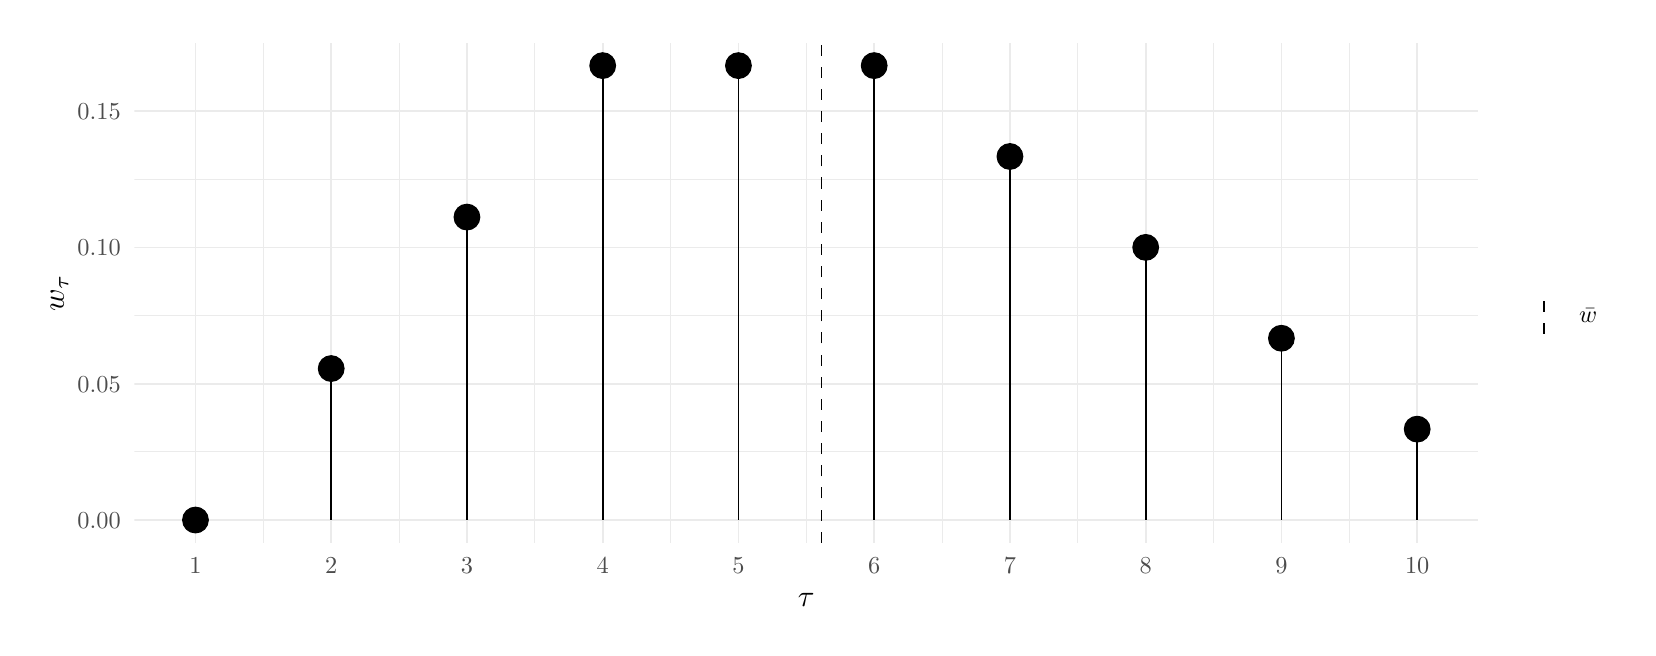
\begin{tikzpicture}[x=1pt,y=1pt]
\definecolor{fillColor}{RGB}{255,255,255}
\path[use as bounding box,fill=fillColor,fill opacity=0.00] (0,0) rectangle (578.16,216.81);
\begin{scope}
\path[clip] ( 38.56, 30.69) rectangle (524.17,211.31);
\definecolor{drawColor}{gray}{0.92}

\path[draw=drawColor,line width= 0.3pt,line join=round] ( 38.56, 63.53) --
	(524.17, 63.53);

\path[draw=drawColor,line width= 0.3pt,line join=round] ( 38.56,112.79) --
	(524.17,112.79);

\path[draw=drawColor,line width= 0.3pt,line join=round] ( 38.56,162.05) --
	(524.17,162.05);

\path[draw=drawColor,line width= 0.3pt,line join=round] ( 85.15, 30.69) --
	( 85.15,211.31);

\path[draw=drawColor,line width= 0.3pt,line join=round] (134.21, 30.69) --
	(134.21,211.31);

\path[draw=drawColor,line width= 0.3pt,line join=round] (183.26, 30.69) --
	(183.26,211.31);

\path[draw=drawColor,line width= 0.3pt,line join=round] (232.31, 30.69) --
	(232.31,211.31);

\path[draw=drawColor,line width= 0.3pt,line join=round] (281.36, 30.69) --
	(281.36,211.31);

\path[draw=drawColor,line width= 0.3pt,line join=round] (330.41, 30.69) --
	(330.41,211.31);

\path[draw=drawColor,line width= 0.3pt,line join=round] (379.47, 30.69) --
	(379.47,211.31);

\path[draw=drawColor,line width= 0.3pt,line join=round] (428.52, 30.69) --
	(428.52,211.31);

\path[draw=drawColor,line width= 0.3pt,line join=round] (477.57, 30.69) --
	(477.57,211.31);

\path[draw=drawColor,line width= 0.6pt,line join=round] ( 38.56, 38.90) --
	(524.17, 38.90);

\path[draw=drawColor,line width= 0.6pt,line join=round] ( 38.56, 88.16) --
	(524.17, 88.16);

\path[draw=drawColor,line width= 0.6pt,line join=round] ( 38.56,137.42) --
	(524.17,137.42);

\path[draw=drawColor,line width= 0.6pt,line join=round] ( 38.56,186.68) --
	(524.17,186.68);

\path[draw=drawColor,line width= 0.6pt,line join=round] ( 60.63, 30.69) --
	( 60.63,211.31);

\path[draw=drawColor,line width= 0.6pt,line join=round] (109.68, 30.69) --
	(109.68,211.31);

\path[draw=drawColor,line width= 0.6pt,line join=round] (158.73, 30.69) --
	(158.73,211.31);

\path[draw=drawColor,line width= 0.6pt,line join=round] (207.78, 30.69) --
	(207.78,211.31);

\path[draw=drawColor,line width= 0.6pt,line join=round] (256.84, 30.69) --
	(256.84,211.31);

\path[draw=drawColor,line width= 0.6pt,line join=round] (305.89, 30.69) --
	(305.89,211.31);

\path[draw=drawColor,line width= 0.6pt,line join=round] (354.94, 30.69) --
	(354.94,211.31);

\path[draw=drawColor,line width= 0.6pt,line join=round] (403.99, 30.69) --
	(403.99,211.31);

\path[draw=drawColor,line width= 0.6pt,line join=round] (453.04, 30.69) --
	(453.04,211.31);

\path[draw=drawColor,line width= 0.6pt,line join=round] (502.10, 30.69) --
	(502.10,211.31);
\definecolor{drawColor}{RGB}{0,0,0}
\definecolor{fillColor}{RGB}{0,0,0}

\path[draw=drawColor,line width= 0.4pt,line join=round,line cap=round,fill=fillColor] ( 60.63, 38.90) circle (  4.64);

\path[draw=drawColor,line width= 0.4pt,line join=round,line cap=round,fill=fillColor] (109.68, 93.63) circle (  4.64);

\path[draw=drawColor,line width= 0.4pt,line join=round,line cap=round,fill=fillColor] (158.73,148.37) circle (  4.64);

\path[draw=drawColor,line width= 0.4pt,line join=round,line cap=round,fill=fillColor] (207.78,203.10) circle (  4.64);

\path[draw=drawColor,line width= 0.4pt,line join=round,line cap=round,fill=fillColor] (256.84,203.10) circle (  4.64);

\path[draw=drawColor,line width= 0.4pt,line join=round,line cap=round,fill=fillColor] (305.89,203.10) circle (  4.64);

\path[draw=drawColor,line width= 0.4pt,line join=round,line cap=round,fill=fillColor] (354.94,170.26) circle (  4.64);

\path[draw=drawColor,line width= 0.4pt,line join=round,line cap=round,fill=fillColor] (403.99,137.42) circle (  4.64);

\path[draw=drawColor,line width= 0.4pt,line join=round,line cap=round,fill=fillColor] (453.04,104.58) circle (  4.64);

\path[draw=drawColor,line width= 0.4pt,line join=round,line cap=round,fill=fillColor] (502.10, 71.74) circle (  4.64);

\path[draw=drawColor,line width= 0.6pt,line join=round] ( 60.63, 38.90) -- ( 60.63, 38.90);

\path[draw=drawColor,line width= 0.6pt,line join=round] (109.68, 93.63) -- (109.68, 38.90);

\path[draw=drawColor,line width= 0.6pt,line join=round] (158.73,148.37) -- (158.73, 38.90);

\path[draw=drawColor,line width= 0.6pt,line join=round] (207.78,203.10) -- (207.78, 38.90);

\path[draw=drawColor,line width= 0.6pt,line join=round] (256.84,203.10) -- (256.84, 38.90);

\path[draw=drawColor,line width= 0.6pt,line join=round] (305.89,203.10) -- (305.89, 38.90);

\path[draw=drawColor,line width= 0.6pt,line join=round] (354.94,170.26) -- (354.94, 38.90);

\path[draw=drawColor,line width= 0.6pt,line join=round] (403.99,137.42) -- (403.99, 38.90);

\path[draw=drawColor,line width= 0.6pt,line join=round] (453.04,104.58) -- (453.04, 38.90);

\path[draw=drawColor,line width= 0.6pt,line join=round] (502.10, 71.74) -- (502.10, 38.90);

\path[draw=drawColor,line width= 0.6pt,dash pattern=on 4pt off 4pt ,line join=round] (286.81, 30.69) -- (286.81,211.31);
\end{scope}
\begin{scope}
\path[clip] (  0.00,  0.00) rectangle (578.16,216.81);
\definecolor{drawColor}{gray}{0.30}

\node[text=drawColor,anchor=base east,inner sep=0pt, outer sep=0pt, scale=  0.88] at ( 33.61, 35.87) {0.00};

\node[text=drawColor,anchor=base east,inner sep=0pt, outer sep=0pt, scale=  0.88] at ( 33.61, 85.13) {0.05};

\node[text=drawColor,anchor=base east,inner sep=0pt, outer sep=0pt, scale=  0.88] at ( 33.61,134.39) {0.10};

\node[text=drawColor,anchor=base east,inner sep=0pt, outer sep=0pt, scale=  0.88] at ( 33.61,183.65) {0.15};
\end{scope}
\begin{scope}
\path[clip] (  0.00,  0.00) rectangle (578.16,216.81);
\definecolor{drawColor}{gray}{0.30}

\node[text=drawColor,anchor=base,inner sep=0pt, outer sep=0pt, scale=  0.88] at ( 60.63, 19.68) {1};

\node[text=drawColor,anchor=base,inner sep=0pt, outer sep=0pt, scale=  0.88] at (109.68, 19.68) {2};

\node[text=drawColor,anchor=base,inner sep=0pt, outer sep=0pt, scale=  0.88] at (158.73, 19.68) {3};

\node[text=drawColor,anchor=base,inner sep=0pt, outer sep=0pt, scale=  0.88] at (207.78, 19.68) {4};

\node[text=drawColor,anchor=base,inner sep=0pt, outer sep=0pt, scale=  0.88] at (256.84, 19.68) {5};

\node[text=drawColor,anchor=base,inner sep=0pt, outer sep=0pt, scale=  0.88] at (305.89, 19.68) {6};

\node[text=drawColor,anchor=base,inner sep=0pt, outer sep=0pt, scale=  0.88] at (354.94, 19.68) {7};

\node[text=drawColor,anchor=base,inner sep=0pt, outer sep=0pt, scale=  0.88] at (403.99, 19.68) {8};

\node[text=drawColor,anchor=base,inner sep=0pt, outer sep=0pt, scale=  0.88] at (453.04, 19.68) {9};

\node[text=drawColor,anchor=base,inner sep=0pt, outer sep=0pt, scale=  0.88] at (502.10, 19.68) {10};
\end{scope}
\begin{scope}
\path[clip] (  0.00,  0.00) rectangle (578.16,216.81);
\definecolor{drawColor}{RGB}{0,0,0}

\node[text=drawColor,anchor=base,inner sep=0pt, outer sep=0pt, scale=  1.10] at (281.36,  7.64) {$\tau$};
\end{scope}
\begin{scope}
\path[clip] (  0.00,  0.00) rectangle (578.16,216.81);
\definecolor{drawColor}{RGB}{0,0,0}

\node[text=drawColor,rotate= 90.00,anchor=base,inner sep=0pt, outer sep=0pt, scale=  1.10] at ( 13.08,121.00) {$w_\tau$};
\end{scope}
\begin{scope}
\path[clip] (  0.00,  0.00) rectangle (578.16,216.81);
\definecolor{drawColor}{RGB}{0,0,0}

\path[draw=drawColor,line width= 0.6pt,dash pattern=on 4pt off 4pt ,line join=round] (547.90,106.16) -- (547.90,120.62);
\end{scope}
\begin{scope}
\path[clip] (  0.00,  0.00) rectangle (578.16,216.81);
\definecolor{drawColor}{RGB}{0,0,0}

\node[text=drawColor,anchor=base west,inner sep=0pt, outer sep=0pt, scale=  0.88] at (560.62,110.36) {$\bar w$};
\end{scope}
\end{tikzpicture}
%
    }
    \caption{Generation time distribution used to estimate reproduction numbers throughout this thesis.}
    \label{fig:generation_time}
\end{figure}

\subsection{Incidence and death data}
In this thesis, we focus on the data available for Germany, provided by the \acrshort{rki} available on Zenodo \citep{RobertKoch-Institut2024SARSCoV2} or GitHub \citep{RobertKoch-Institut2024SARSCoV2a}. In these repositories, the \acrshort{rki} publishes daily data on the number of cases in the aforementioned strata. On days, data has not been published to Zenodo or GitHub, e.g. for May 31st, 2020. In this case, we use the data provided by the ard-data RKI-archive on GitHub \citep{MichaelKreil2022RKICoronaDatenArchiv}. 

This data contains the following information for each case and death:
\begin{itemize}
    \item the county (Landkreis) of the case,
    \item sex (male, female or unknown), and age group (00-04, 05-14, 15-34, 35-59, 60-79, 80+, unknown),
    \item the dates of reporting (Meldedatum) and symptom onset (Refdatum), as well as
    \item meta-information on whether the case was already present in the past dataset.
\end{itemize}

The dates of reporting and symptom onset are of particular importance: the date of reporting is the date that the local health authorities become aware of the case, which may be several days after the symptom onset or infection date, but also several days before the \acrshort{rki} is aware of the case. Thus, there are several dates of interest, ordered roughly by occurrence: 
\begin{itemize}
    \item the date of infection, 
    \item the date of symptom onset (if the occurs), 
    \item the date of reporting to the local health authorities,
    \item the date of reporting to the \acrshort{rki} and potentially,
    \item the date of death.
\end{itemize}
Exceptions to this order include the possibility that the date of death could occur before any of the two reporting dates and symptom onset could begin only after the first date of reporting, i.e. because testing is due to contact tracing.

The date of infection is generally unknown. While the date of symptom onset is close to the date of infection, unfortunately, it is only known for roughly $25\%$ of the reported cases. Therefore, we restrict our analyses to the date of reporting. \citep{AnDerHeiden2020Schatzung} use multiple imputation to address this problem; however, this method assumes that the symptom onset dates are missing completely at random, which is questionable as asymptomatic infections will produce no date of symptom onset. There can be considerable delay between the two reporting dates, as we will explore later, see, e.g., \Cref{fig:reporting_delays_cases,fig:survival_function_rep_tri_incidences}.

We restrict ourselves to data available from April 1st, 2020. This dataset already includes cases with earlier reporting date. Additionally, we consider only data reported up to and including May 5th 2023, the date when the WHO declared \acrshort{c19} no longer a global health emergency. \Cref{fig:cases_germany} shows the number of daily reported cases (\textbf{A}) and deaths (\textbf{B}) with a weekly running mean. Apparent from this figure is the considerable day-to-day variation, the so-called weekday effect. As the reporting date is tied to the working hours of the local health authorities, fewer cases are processed, and thus reported, on weekends and more during the week. The weekday effect is less pronounced for the symptom onset date, if it is known (figure not shown). 

We want to highlight two periods of irregularities during the early stage of the epidemic, magnified in \Cref{fig:cases_germany} \textbf{A}. The first concerns a local outbreak in a German meat processing plant \citep{Gunther2020SARSCoV2}. Over two weeks in early June, $1\,413$ positive cases were reported for Gütersloh county. Due to the low number of reported cases everywhere else, this locally confined outbreak is visible even when aggregating over all counties in Germany. \todo{ref this later}
The second period concerns the Christmas holiday break, where we observe a sudden decline in reported cases, compensated by a large influx in cases in the second week of January. Due to the holiday leave, we'd expect this drop in cases to be related to fewer staff working at the local health authorities, rather than a true decrease in cases. Similar patterns are visible for easter 2021 and Christmas 2021. 

\begin{figure}
    \resizebox{\textwidth}{!}{%
        % Created by tikzDevice version 0.12.6 on 2024-08-02 11:25:42
% !TEX encoding = UTF-8 Unicode
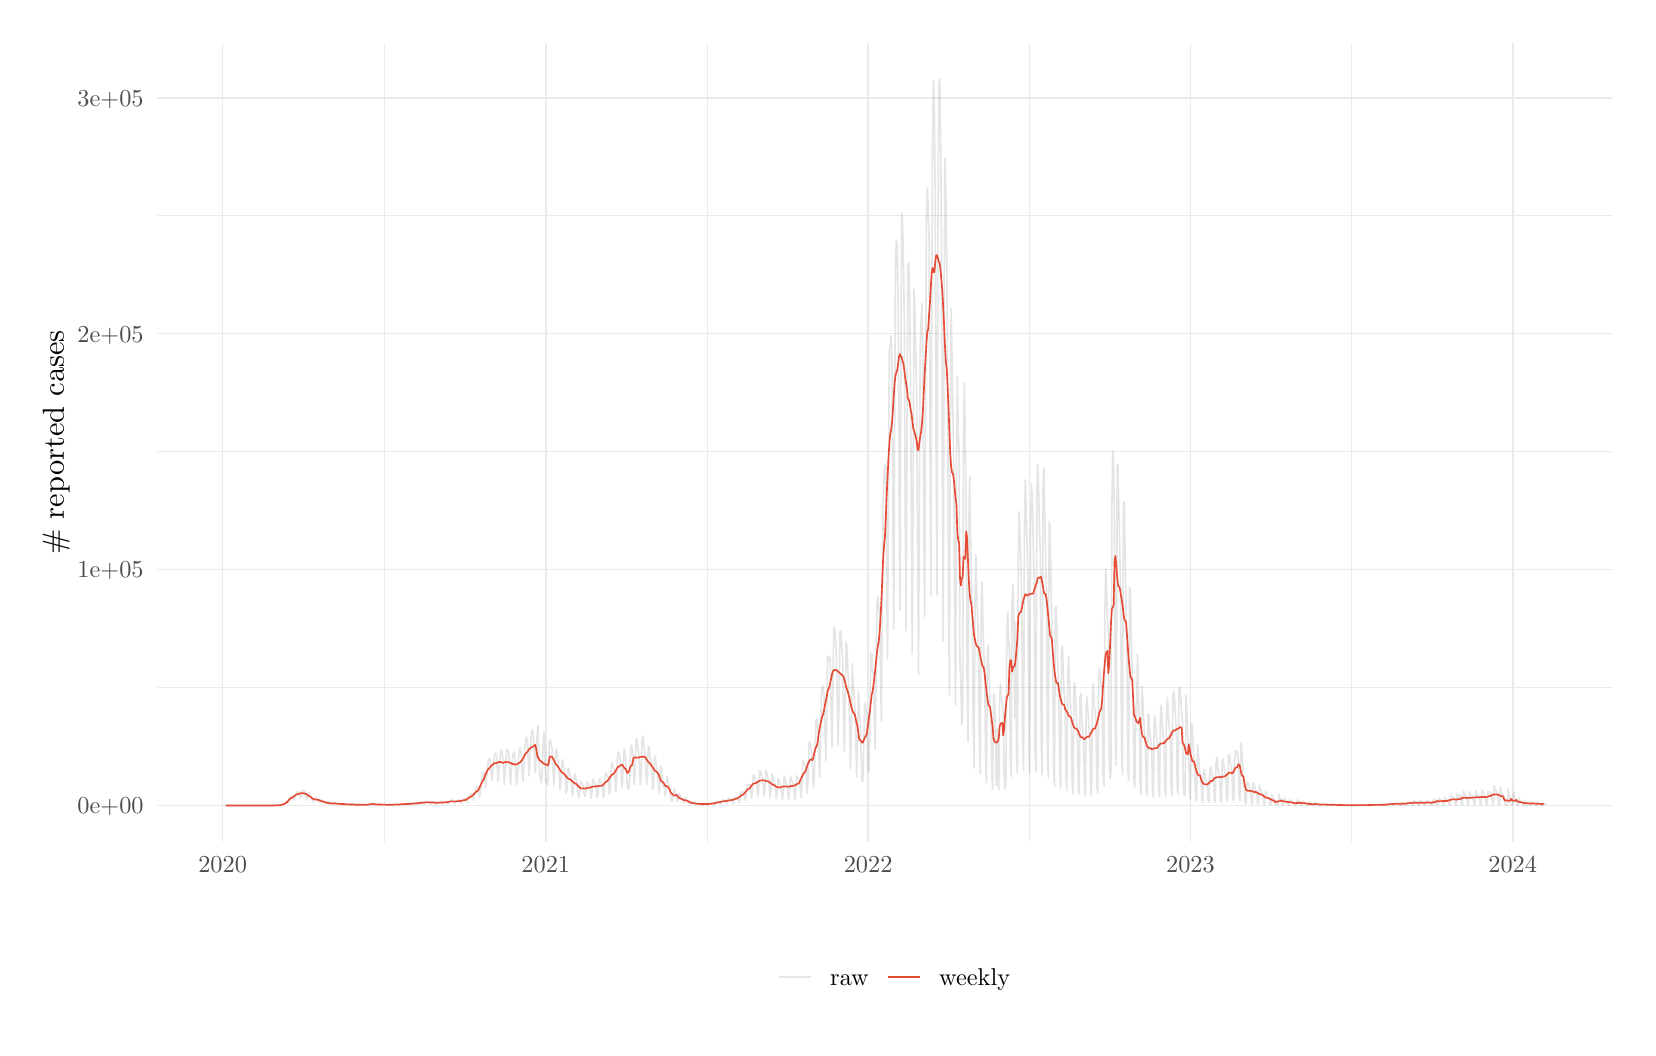
\begin{tikzpicture}[x=1pt,y=1pt]
\definecolor{fillColor}{RGB}{255,255,255}
\path[use as bounding box,fill=fillColor,fill opacity=0.00] (0,0) rectangle (578.16,361.35);
\begin{scope}
\path[clip] ( 46.86, 67.14) rectangle (572.66,355.85);
\definecolor{drawColor}{gray}{0.92}

\path[draw=drawColor,line width= 0.3pt,line join=round] ( 46.86,122.89) --
	(572.66,122.89);

\path[draw=drawColor,line width= 0.3pt,line join=round] ( 46.86,208.15) --
	(572.66,208.15);

\path[draw=drawColor,line width= 0.3pt,line join=round] ( 46.86,293.41) --
	(572.66,293.41);

\path[draw=drawColor,line width= 0.3pt,line join=round] (128.84, 67.14) --
	(128.84,355.85);

\path[draw=drawColor,line width= 0.3pt,line join=round] (245.47, 67.14) --
	(245.47,355.85);

\path[draw=drawColor,line width= 0.3pt,line join=round] (361.93, 67.14) --
	(361.93,355.85);

\path[draw=drawColor,line width= 0.3pt,line join=round] (478.40, 67.14) --
	(478.40,355.85);

\path[draw=drawColor,line width= 0.6pt,line join=round] ( 46.86, 80.26) --
	(572.66, 80.26);

\path[draw=drawColor,line width= 0.6pt,line join=round] ( 46.86,165.52) --
	(572.66,165.52);

\path[draw=drawColor,line width= 0.6pt,line join=round] ( 46.86,250.78) --
	(572.66,250.78);

\path[draw=drawColor,line width= 0.6pt,line join=round] ( 46.86,336.04) --
	(572.66,336.04);

\path[draw=drawColor,line width= 0.6pt,line join=round] ( 70.44, 67.14) --
	( 70.44,355.85);

\path[draw=drawColor,line width= 0.6pt,line join=round] (187.23, 67.14) --
	(187.23,355.85);

\path[draw=drawColor,line width= 0.6pt,line join=round] (303.70, 67.14) --
	(303.70,355.85);

\path[draw=drawColor,line width= 0.6pt,line join=round] (420.17, 67.14) --
	(420.17,355.85);

\path[draw=drawColor,line width= 0.6pt,line join=round] (536.63, 67.14) --
	(536.63,355.85);
\definecolor{drawColor}{RGB}{0,0,0}

\path[draw=drawColor,draw opacity=0.10,line width= 0.6pt,line join=round] ( 70.76, 80.26) --
	( 71.08, 80.26) --
	( 71.40, 80.26) --
	( 71.72, 80.26) --
	( 72.04, 80.26) --
	( 72.36, 80.26) --
	( 72.68, 80.26) --
	( 73.00, 80.26) --
	( 73.32, 80.26) --
	( 73.64, 80.26) --
	( 73.95, 80.26) --
	( 74.27, 80.26) --
	( 74.59, 80.26) --
	( 74.91, 80.26) --
	( 75.23, 80.26) --
	( 75.55, 80.26) --
	( 75.87, 80.26) --
	( 76.19, 80.26) --
	( 76.51, 80.26) --
	( 76.83, 80.26) --
	( 77.15, 80.26) --
	( 77.46, 80.26) --
	( 77.78, 80.26) --
	( 78.10, 80.26) --
	( 78.42, 80.26) --
	( 78.74, 80.26) --
	( 79.06, 80.26) --
	( 79.38, 80.26) --
	( 79.70, 80.26) --
	( 80.02, 80.27) --
	( 80.34, 80.26) --
	( 80.66, 80.26) --
	( 80.97, 80.26) --
	( 81.29, 80.27) --
	( 81.61, 80.26) --
	( 81.93, 80.26) --
	( 82.25, 80.26) --
	( 82.57, 80.26) --
	( 82.89, 80.26) --
	( 83.21, 80.26) --
	( 83.53, 80.26) --
	( 83.85, 80.26) --
	( 84.17, 80.26) --
	( 84.48, 80.26) --
	( 84.80, 80.26) --
	( 85.12, 80.26) --
	( 85.44, 80.26) --
	( 85.76, 80.26) --
	( 86.08, 80.26) --
	( 86.40, 80.26) --
	( 86.72, 80.26) --
	( 87.04, 80.26) --
	( 87.36, 80.26) --
	( 87.68, 80.26) --
	( 87.99, 80.27) --
	( 88.31, 80.27) --
	( 88.63, 80.28) --
	( 88.95, 80.30) --
	( 89.27, 80.28) --
	( 89.59, 80.29) --
	( 89.91, 80.30) --
	( 90.23, 80.34) --
	( 90.55, 80.40) --
	( 90.87, 80.42) --
	( 91.19, 80.42) --
	( 91.50, 80.38) --
	( 91.82, 80.35) --
	( 92.14, 80.56) --
	( 92.46, 80.77) --
	( 92.78, 80.91) --
	( 93.10, 81.11) --
	( 93.42, 81.51) --
	( 93.74, 81.37) --
	( 94.06, 81.10) --
	( 94.38, 82.00) --
	( 94.70, 82.85) --
	( 95.01, 83.34) --
	( 95.33, 83.72) --
	( 95.65, 83.72) --
	( 95.97, 83.13) --
	( 96.29, 82.19) --
	( 96.61, 83.44) --
	( 96.93, 84.42) --
	( 97.25, 85.11) --
	( 97.57, 85.30) --
	( 97.89, 85.36) --
	( 98.21, 84.29) --
	( 98.52, 82.89) --
	( 98.84, 83.79) --
	( 99.16, 85.43) --
	( 99.48, 85.60) --
	( 99.80, 85.85) --
	(100.12, 85.54) --
	(100.44, 83.96) --
	(100.76, 82.42) --
	(101.08, 83.39) --
	(101.40, 84.69) --
	(101.72, 84.77) --
	(102.03, 84.45) --
	(102.35, 83.12) --
	(102.67, 82.72) --
	(102.99, 81.86) --
	(103.31, 81.63) --
	(103.63, 82.37) --
	(103.95, 83.10) --
	(104.27, 83.18) --
	(104.59, 82.86) --
	(104.91, 82.06) --
	(105.23, 81.44) --
	(105.54, 81.72) --
	(105.86, 82.13) --
	(106.18, 82.39) --
	(106.50, 82.05) --
	(106.82, 81.89) --
	(107.14, 81.35) --
	(107.46, 80.86) --
	(107.78, 81.21) --
	(108.10, 81.52) --
	(108.42, 81.48) --
	(108.74, 81.51) --
	(109.05, 81.05) --
	(109.37, 80.79) --
	(109.69, 80.62) --
	(110.01, 80.88) --
	(110.33, 81.20) --
	(110.65, 81.30) --
	(110.97, 81.29) --
	(111.29, 81.10) --
	(111.61, 80.84) --
	(111.93, 80.55) --
	(112.25, 80.85) --
	(112.56, 80.99) --
	(112.88, 81.04) --
	(113.20, 80.96) --
	(113.52, 80.89) --
	(113.84, 80.66) --
	(114.16, 80.53) --
	(114.48, 80.72) --
	(114.80, 80.89) --
	(115.12, 80.97) --
	(115.44, 80.62) --
	(115.76, 80.71) --
	(116.07, 80.55) --
	(116.39, 80.45) --
	(116.71, 80.61) --
	(117.03, 80.79) --
	(117.35, 80.82) --
	(117.67, 80.71) --
	(117.99, 80.64) --
	(118.31, 80.58) --
	(118.63, 80.41) --
	(118.95, 80.38) --
	(119.27, 80.52) --
	(119.58, 80.69) --
	(119.90, 80.71) --
	(120.22, 80.63) --
	(120.54, 80.51) --
	(120.86, 80.40) --
	(121.18, 80.51) --
	(121.50, 80.63) --
	(121.82, 80.70) --
	(122.14, 80.50) --
	(122.46, 80.56) --
	(122.78, 80.52) --
	(123.09, 80.41) --
	(123.41, 80.48) --
	(123.73, 80.70) --
	(124.05, 81.00) --
	(124.37, 80.92) --
	(124.69, 81.11) --
	(125.01, 80.75) --
	(125.33, 80.45) --
	(125.65, 80.64) --
	(125.97, 80.72) --
	(126.29, 80.70) --
	(126.60, 80.75) --
	(126.92, 80.75) --
	(127.24, 80.54) --
	(127.56, 80.43) --
	(127.88, 80.62) --
	(128.20, 80.65) --
	(128.52, 80.67) --
	(128.84, 80.66) --
	(129.16, 80.63) --
	(129.48, 80.51) --
	(129.80, 80.39) --
	(130.11, 80.54) --
	(130.43, 80.60) --
	(130.75, 80.65) --
	(131.07, 80.62) --
	(131.39, 80.63) --
	(131.71, 80.50) --
	(132.03, 80.38) --
	(132.35, 80.54) --
	(132.67, 80.66) --
	(132.99, 80.73) --
	(133.31, 80.74) --
	(133.62, 80.71) --
	(133.94, 80.64) --
	(134.26, 80.42) --
	(134.58, 80.65) --
	(134.90, 80.71) --
	(135.22, 80.86) --
	(135.54, 80.85) --
	(135.86, 80.95) --
	(136.18, 80.73) --
	(136.50, 80.44) --
	(136.82, 80.71) --
	(137.13, 80.91) --
	(137.45, 81.04) --
	(137.77, 81.00) --
	(138.09, 81.04) --
	(138.41, 80.74) --
	(138.73, 80.52) --
	(139.05, 80.94) --
	(139.37, 81.07) --
	(139.69, 81.21) --
	(140.01, 81.26) --
	(140.33, 81.12) --
	(140.64, 80.87) --
	(140.96, 80.53) --
	(141.28, 81.20) --
	(141.60, 81.28) --
	(141.92, 81.58) --
	(142.24, 81.55) --
	(142.56, 81.44) --
	(142.88, 80.91) --
	(143.20, 80.68) --
	(143.52, 81.58) --
	(143.84, 81.57) --
	(144.15, 81.76) --
	(144.47, 81.64) --
	(144.79, 81.68) --
	(145.11, 81.05) --
	(145.43, 80.74) --
	(145.75, 81.48) --
	(146.07, 81.53) --
	(146.39, 81.65) --
	(146.71, 81.58) --
	(147.03, 81.45) --
	(147.35, 80.97) --
	(147.66, 80.72) --
	(147.98, 81.27) --
	(148.30, 81.39) --
	(148.62, 81.47) --
	(148.94, 81.55) --
	(149.26, 81.54) --
	(149.58, 81.21) --
	(149.90, 80.76) --
	(150.22, 81.47) --
	(150.54, 81.44) --
	(150.86, 81.75) --
	(151.17, 81.62) --
	(151.49, 81.68) --
	(151.81, 81.31) --
	(152.13, 80.91) --
	(152.45, 81.53) --
	(152.77, 81.97) --
	(153.09, 82.12) --
	(153.41, 82.28) --
	(153.73, 82.11) --
	(154.05, 81.45) --
	(154.37, 80.85) --
	(154.68, 81.67) --
	(155.00, 81.81) --
	(155.32, 82.15) --
	(155.64, 82.30) --
	(155.96, 82.25) --
	(156.28, 81.78) --
	(156.60, 81.01) --
	(156.92, 81.83) --
	(157.24, 82.11) --
	(157.56, 82.60) --
	(157.88, 82.76) --
	(158.19, 82.76) --
	(158.51, 82.14) --
	(158.83, 81.25) --
	(159.15, 82.32) --
	(159.47, 83.32) --
	(159.79, 84.10) --
	(160.11, 84.25) --
	(160.43, 84.58) --
	(160.75, 83.35) --
	(161.07, 82.20) --
	(161.39, 83.84) --
	(161.70, 84.84) --
	(162.02, 86.44) --
	(162.34, 87.00) --
	(162.66, 87.06) --
	(162.98, 85.10) --
	(163.30, 83.40) --
	(163.62, 85.77) --
	(163.94, 88.31) --
	(164.26, 90.84) --
	(164.58, 92.12) --
	(164.90, 92.24) --
	(165.21, 89.72) --
	(165.53, 86.62) --
	(165.85, 90.52) --
	(166.17, 93.86) --
	(166.49, 96.67) --
	(166.81, 97.18) --
	(167.13, 96.81) --
	(167.45, 92.19) --
	(167.77, 89.25) --
	(168.09, 93.26) --
	(168.41, 96.75) --
	(168.72, 98.34) --
	(169.04, 99.26) --
	(169.36, 98.65) --
	(169.68, 93.84) --
	(170.00, 88.90) --
	(170.32, 93.90) --
	(170.64, 96.99) --
	(170.96, 99.63) --
	(171.28,100.35) --
	(171.60, 98.44) --
	(171.92, 93.74) --
	(172.23, 87.81) --
	(172.55, 92.80) --
	(172.87, 97.64) --
	(173.19,100.45) --
	(173.51,100.52) --
	(173.83, 99.29) --
	(174.15, 92.85) --
	(174.47, 87.77) --
	(174.79, 93.11) --
	(175.11, 96.81) --
	(175.43, 99.04) --
	(175.74, 99.65) --
	(176.06, 97.45) --
	(176.38, 93.00) --
	(176.70, 87.75) --
	(177.02, 91.60) --
	(177.34, 96.69) --
	(177.66,100.04) --
	(177.98,101.11) --
	(178.30, 99.16) --
	(178.62, 93.66) --
	(178.94, 88.98) --
	(179.25, 94.26) --
	(179.57, 99.72) --
	(179.89,103.81) --
	(180.21,105.01) --
	(180.53,103.50) --
	(180.85, 97.85) --
	(181.17, 90.92) --
	(181.49, 96.47) --
	(181.81,103.20) --
	(182.13,107.01) --
	(182.45,107.51) --
	(182.76,105.58) --
	(183.08, 98.79) --
	(183.40, 92.13) --
	(183.72, 97.55) --
	(184.04,104.94) --
	(184.36,109.20) --
	(184.68, 98.27) --
	(185.00, 91.47) --
	(185.32, 90.11) --
	(185.64, 88.63) --
	(185.96, 93.65) --
	(186.27,103.75) --
	(186.59,106.74) --
	(186.91, 96.94) --
	(187.23, 89.00) --
	(187.55, 88.79) --
	(187.87, 87.79) --
	(188.19, 92.50) --
	(188.51,103.64) --
	(188.83,104.08) --
	(189.15,102.51) --
	(189.47,101.19) --
	(189.78, 94.47) --
	(190.10, 87.48) --
	(190.42, 91.77) --
	(190.74, 99.52) --
	(191.06,100.82) --
	(191.38, 97.65) --
	(191.70, 95.87) --
	(192.02, 91.71) --
	(192.34, 85.88) --
	(192.66, 88.08) --
	(192.98, 96.01) --
	(193.29, 96.86) --
	(193.61, 94.61) --
	(193.93, 93.08) --
	(194.25, 90.13) --
	(194.57, 84.54) --
	(194.89, 86.02) --
	(195.21, 93.49) --
	(195.53, 93.75) --
	(195.85, 91.65) --
	(196.17, 90.98) --
	(196.49, 88.75) --
	(196.80, 83.85) --
	(197.12, 85.26) --
	(197.44, 90.75) --
	(197.76, 91.71) --
	(198.08, 90.08) --
	(198.40, 88.81) --
	(198.72, 87.41) --
	(199.04, 82.90) --
	(199.36, 83.84) --
	(199.68, 88.01) --
	(200.00, 89.03) --
	(200.31, 88.25) --
	(200.63, 87.54) --
	(200.95, 85.03) --
	(201.27, 83.47) --
	(201.59, 84.01) --
	(201.91, 88.13) --
	(202.23, 88.78) --
	(202.55, 88.12) --
	(202.87, 87.69) --
	(203.19, 86.89) --
	(203.51, 82.84) --
	(203.82, 84.02) --
	(204.14, 88.93) --
	(204.46, 89.90) --
	(204.78, 88.70) --
	(205.10, 88.34) --
	(205.42, 86.79) --
	(205.74, 83.21) --
	(206.06, 84.26) --
	(206.38, 89.61) --
	(206.70, 89.91) --
	(207.02, 88.90) --
	(207.33, 88.49) --
	(207.65, 87.34) --
	(207.97, 83.13) --
	(208.29, 84.40) --
	(208.61, 90.08) --
	(208.93, 92.20) --
	(209.25, 91.48) --
	(209.57, 90.97) --
	(209.89, 89.19) --
	(210.21, 84.39) --
	(210.53, 86.10) --
	(210.84, 93.72) --
	(211.16, 95.92) --
	(211.48, 94.53) --
	(211.80, 93.65) --
	(212.12, 91.53) --
	(212.44, 85.34) --
	(212.76, 87.85) --
	(213.08, 96.85) --
	(213.40, 99.56) --
	(213.72, 98.94) --
	(214.04, 97.35) --
	(214.35, 93.72) --
	(214.67, 86.73) --
	(214.99, 89.64) --
	(215.31, 97.64) --
	(215.63,100.71) --
	(215.95, 98.52) --
	(216.27, 93.46) --
	(216.59, 89.30) --
	(216.91, 86.35) --
	(217.23, 86.25) --
	(217.55, 90.07) --
	(217.86,100.49) --
	(218.18,102.22) --
	(218.50,100.12) --
	(218.82, 95.66) --
	(219.14, 87.81) --
	(219.46, 90.59) --
	(219.78,103.05) --
	(220.10,104.61) --
	(220.42,101.63) --
	(220.74, 99.94) --
	(221.06, 95.34) --
	(221.37, 87.77) --
	(221.69, 90.75) --
	(222.01,104.10) --
	(222.33,105.30) --
	(222.65,101.94) --
	(222.97, 99.84) --
	(223.29, 95.61) --
	(223.61, 87.65) --
	(223.93, 90.65) --
	(224.25,101.79) --
	(224.57,101.58) --
	(224.88, 98.51) --
	(225.20, 96.59) --
	(225.52, 93.09) --
	(225.84, 85.93) --
	(226.16, 88.03) --
	(226.48, 98.14) --
	(226.80, 98.03) --
	(227.12, 94.88) --
	(227.44, 93.44) --
	(227.76, 90.50) --
	(228.08, 84.80) --
	(228.39, 86.56) --
	(228.71, 94.54) --
	(229.03, 94.30) --
	(229.35, 88.50) --
	(229.67, 86.77) --
	(229.99, 87.59) --
	(230.31, 83.90) --
	(230.63, 84.73) --
	(230.95, 90.76) --
	(231.27, 89.90) --
	(231.59, 87.44) --
	(231.90, 86.72) --
	(232.22, 85.23) --
	(232.54, 81.97) --
	(232.86, 81.80) --
	(233.18, 83.39) --
	(233.50, 86.35) --
	(233.82, 86.05) --
	(234.14, 84.67) --
	(234.46, 83.41) --
	(234.78, 81.63) --
	(235.10, 82.34) --
	(235.41, 84.61) --
	(235.73, 84.09) --
	(236.05, 82.76) --
	(236.37, 82.20) --
	(236.69, 82.23) --
	(237.01, 81.23) --
	(237.33, 81.73) --
	(237.65, 83.28) --
	(237.97, 82.70) --
	(238.29, 82.21) --
	(238.61, 81.83) --
	(238.92, 81.38) --
	(239.24, 80.70) --
	(239.56, 81.06) --
	(239.88, 81.71) --
	(240.20, 81.49) --
	(240.52, 81.25) --
	(240.84, 81.14) --
	(241.16, 80.89) --
	(241.48, 80.50) --
	(241.80, 80.78) --
	(242.12, 81.17) --
	(242.43, 81.03) --
	(242.75, 80.97) --
	(243.07, 80.89) --
	(243.39, 80.67) --
	(243.71, 80.45) --
	(244.03, 80.71) --
	(244.35, 81.03) --
	(244.67, 81.00) --
	(244.99, 80.87) --
	(245.31, 80.83) --
	(245.63, 80.70) --
	(245.94, 80.44) --
	(246.26, 80.74) --
	(246.58, 81.17) --
	(246.90, 81.08) --
	(247.22, 81.08) --
	(247.54, 81.07) --
	(247.86, 80.94) --
	(248.18, 80.53) --
	(248.50, 80.95) --
	(248.82, 81.77) --
	(249.14, 81.65) --
	(249.45, 81.56) --
	(249.77, 81.64) --
	(250.09, 81.36) --
	(250.41, 80.69) --
	(250.73, 81.48) --
	(251.05, 82.26) --
	(251.37, 82.22) --
	(251.69, 82.16) --
	(252.01, 82.07) --
	(252.33, 81.62) --
	(252.65, 80.81) --
	(252.96, 81.68) --
	(253.28, 82.90) --
	(253.60, 82.69) --
	(253.92, 82.51) --
	(254.24, 82.42) --
	(254.56, 81.94) --
	(254.88, 80.93) --
	(255.20, 82.07) --
	(255.52, 83.47) --
	(255.84, 83.28) --
	(256.16, 83.27) --
	(256.47, 83.28) --
	(256.79, 82.64) --
	(257.11, 81.24) --
	(257.43, 82.76) --
	(257.75, 85.01) --
	(258.07, 85.08) --
	(258.39, 84.91) --
	(258.71, 85.20) --
	(259.03, 84.22) --
	(259.35, 82.03) --
	(259.67, 84.12) --
	(259.98, 87.87) --
	(260.30, 87.73) --
	(260.62, 87.67) --
	(260.94, 87.80) --
	(261.26, 86.08) --
	(261.58, 82.90) --
	(261.90, 85.87) --
	(262.22, 91.26) --
	(262.54, 91.11) --
	(262.86, 90.18) --
	(263.17, 89.13) --
	(263.49, 87.43) --
	(263.81, 83.45) --
	(264.13, 86.31) --
	(264.45, 92.69) --
	(264.77, 92.83) --
	(265.09, 91.11) --
	(265.41, 90.56) --
	(265.73, 88.34) --
	(266.05, 83.71) --
	(266.37, 86.24) --
	(266.68, 93.15) --
	(267.00, 92.33) --
	(267.32, 90.83) --
	(267.64, 89.76) --
	(267.96, 87.56) --
	(268.28, 83.06) --
	(268.60, 86.13) --
	(268.92, 91.68) --
	(269.24, 90.69) --
	(269.56, 89.02) --
	(269.88, 87.84) --
	(270.19, 86.26) --
	(270.51, 82.63) --
	(270.83, 84.88) --
	(271.15, 89.86) --
	(271.47, 89.18) --
	(271.79, 88.01) --
	(272.11, 87.44) --
	(272.43, 85.68) --
	(272.75, 82.52) --
	(273.07, 85.18) --
	(273.39, 91.05) --
	(273.70, 89.96) --
	(274.02, 88.36) --
	(274.34, 87.42) --
	(274.66, 85.51) --
	(274.98, 82.52) --
	(275.30, 85.10) --
	(275.62, 90.68) --
	(275.94, 89.74) --
	(276.26, 88.91) --
	(276.58, 88.12) --
	(276.90, 86.25) --
	(277.21, 82.51) --
	(277.53, 85.60) --
	(277.85, 91.04) --
	(278.17, 90.55) --
	(278.49, 89.93) --
	(278.81, 89.77) --
	(279.13, 87.50) --
	(279.45, 83.17) --
	(279.77, 87.20) --
	(280.09, 96.60) --
	(280.41, 95.59) --
	(280.72, 95.01) --
	(281.04, 94.48) --
	(281.36, 91.59) --
	(281.68, 84.68) --
	(282.00, 90.38) --
	(282.32,102.76) --
	(282.64,103.54) --
	(282.96,101.02) --
	(283.28, 99.50) --
	(283.60, 94.82) --
	(283.92, 86.62) --
	(284.23, 90.05) --
	(284.55,101.07) --
	(284.87,111.08) --
	(285.19,111.36) --
	(285.51,109.03) --
	(285.83,100.53) --
	(286.15, 90.37) --
	(286.47,100.98) --
	(286.79,120.50) --
	(287.11,123.62) --
	(287.43,122.67) --
	(287.74,119.55) --
	(288.06,109.23) --
	(288.38, 96.49) --
	(288.70,109.75) --
	(289.02,133.98) --
	(289.34,134.14) --
	(289.66,132.46) --
	(289.98,133.59) --
	(290.30,116.35) --
	(290.62,101.39) --
	(290.94,120.05) --
	(291.25,143.82) --
	(291.57,144.82) --
	(291.89,141.53) --
	(292.21,134.90) --
	(292.53,118.57) --
	(292.85,102.04) --
	(293.17,118.07) --
	(293.49,143.02) --
	(293.81,143.37) --
	(294.13,138.24) --
	(294.45,133.57) --
	(294.76,116.48) --
	(295.08, 99.93) --
	(295.40,116.51) --
	(295.72,139.38) --
	(296.04,137.56) --
	(296.36,129.43) --
	(296.68,123.86) --
	(297.00,109.78) --
	(297.32, 93.51) --
	(297.64,107.20) --
	(297.96,131.59) --
	(298.27,124.96) --
	(298.59,120.56) --
	(298.91,115.44) --
	(299.23,104.58) --
	(299.55, 90.69) --
	(299.87,103.25) --
	(300.19,121.40) --
	(300.51,115.15) --
	(300.83,110.09) --
	(301.15, 98.93) --
	(301.47, 89.15) --
	(301.78, 89.14) --
	(302.10,101.13) --
	(302.42,117.22) --
	(302.74,115.77) --
	(303.06,115.61) --
	(303.38,104.96) --
	(303.70, 92.39) --
	(304.02, 92.69) --
	(304.34,110.92) --
	(304.66,135.29) --
	(304.98,135.24) --
	(305.29,128.25) --
	(305.61,127.91) --
	(305.93,111.85) --
	(306.25,100.51) --
	(306.57,126.06) --
	(306.89,153.68) --
	(307.21,155.64) --
	(307.53,151.95) --
	(307.85,149.14) --
	(308.17,129.16) --
	(308.49,110.63) --
	(308.80,150.81) --
	(309.12,188.35) --
	(309.44,199.79) --
	(309.76,203.56) --
	(310.08,203.18) --
	(310.40,162.40) --
	(310.72,133.10) --
	(311.04,199.09) --
	(311.36,245.23) --
	(311.68,246.39) --
	(312.00,250.05) --
	(312.31,240.47) --
	(312.63,186.72) --
	(312.95,144.08) --
	(313.27,216.01) --
	(313.59,277.11) --
	(313.91,284.48) --
	(314.23,282.41) --
	(314.55,259.14) --
	(314.87,193.93) --
	(315.19,150.95) --
	(315.51,232.17) --
	(315.82,294.25) --
	(316.14,291.23) --
	(316.46,276.44) --
	(316.78,256.46) --
	(317.10,184.72) --
	(317.42,143.56) --
	(317.74,215.66) --
	(318.06,275.43) --
	(318.38,276.50) --
	(318.70,262.11) --
	(319.02,232.91) --
	(319.33,182.50) --
	(319.65,135.05) --
	(319.97,199.39) --
	(320.29,266.81) --
	(320.61,257.84) --
	(320.93,242.29) --
	(321.25,226.76) --
	(321.57,173.03) --
	(321.89,127.58) --
	(322.21,190.06) --
	(322.53,245.62) --
	(322.84,255.51) --
	(323.16,261.67) --
	(323.48,242.40) --
	(323.80,184.69) --
	(324.12,148.39) --
	(324.44,221.77) --
	(324.76,291.63) --
	(325.08,303.32) --
	(325.40,297.22) --
	(325.72,283.83) --
	(326.04,213.29) --
	(326.35,156.20) --
	(326.67,257.57) --
	(326.99,323.35) --
	(327.31,342.30) --
	(327.63,331.63) --
	(327.95,297.46) --
	(328.27,202.42) --
	(328.59,156.43) --
	(328.91,282.96) --
	(329.23,340.23) --
	(329.55,342.73) --
	(329.86,324.23) --
	(330.18,288.47) --
	(330.50,198.21) --
	(330.82,139.71) --
	(331.14,256.65) --
	(331.46,314.19) --
	(331.78,301.87) --
	(332.10,278.08) --
	(332.42,235.46) --
	(332.74,159.67) --
	(333.06,119.99) --
	(333.37,212.69) --
	(333.69,260.01) --
	(334.01,241.35) --
	(334.33,223.26) --
	(334.65,202.07) --
	(334.97,145.16) --
	(335.29,116.70) --
	(335.61,199.92) --
	(335.93,235.58) --
	(336.25,215.75) --
	(336.57,208.64) --
	(336.88,132.23) --
	(337.20,124.59) --
	(337.52,109.45) --
	(337.84,111.75) --
	(338.16,215.54) --
	(338.48,233.26) --
	(338.80,213.00) --
	(339.12,182.13) --
	(339.44,126.68) --
	(339.76,103.27) --
	(340.08,181.57) --
	(340.39,199.08) --
	(340.71,178.70) --
	(341.03,160.98) --
	(341.35,146.99) --
	(341.67,109.25) --
	(341.99, 93.78) --
	(342.31,154.02) --
	(342.63,171.05) --
	(342.95,156.86) --
	(343.27,148.78) --
	(343.59,137.52) --
	(343.90,103.27) --
	(344.22, 91.65) --
	(344.54,152.58) --
	(344.86,161.12) --
	(345.18,146.04) --
	(345.50,135.64) --
	(345.82,128.78) --
	(346.14, 97.41) --
	(346.46, 88.49) --
	(346.78,136.23) --
	(347.10,138.30) --
	(347.41,126.12) --
	(347.73,118.00) --
	(348.05,114.32) --
	(348.37, 92.04) --
	(348.69, 86.18) --
	(349.01,120.39) --
	(349.33,120.06) --
	(349.65,110.42) --
	(349.97, 87.37) --
	(350.29,108.06) --
	(350.61, 89.32) --
	(350.92, 85.77) --
	(351.24,120.24) --
	(351.56,124.19) --
	(351.88,118.58) --
	(352.20,116.42) --
	(352.52,113.89) --
	(352.84, 91.15) --
	(353.16, 86.34) --
	(353.48, 88.26) --
	(353.80,141.05) --
	(354.12,150.24) --
	(354.43,141.04) --
	(354.75,135.93) --
	(355.07, 97.12) --
	(355.39, 90.76) --
	(355.71,154.47) --
	(356.03,160.05) --
	(356.35,150.07) --
	(356.67,112.05) --
	(356.99,146.38) --
	(357.31,100.01) --
	(357.63, 91.60) --
	(357.94,170.26) --
	(358.26,186.47) --
	(358.58,177.05) --
	(358.90,166.69) --
	(359.22,154.60) --
	(359.54,103.46) --
	(359.86, 92.88) --
	(360.18,179.93) --
	(360.50,197.99) --
	(360.82,186.93) --
	(361.14,174.27) --
	(361.45,161.14) --
	(361.77,100.65) --
	(362.09, 91.84) --
	(362.41,183.23) --
	(362.73,196.71) --
	(363.05,188.91) --
	(363.37,174.78) --
	(363.69,161.77) --
	(364.01,100.42) --
	(364.33, 92.51) --
	(364.65,191.92) --
	(364.96,203.54) --
	(365.28,195.86) --
	(365.60,179.95) --
	(365.92,172.87) --
	(366.24,101.85) --
	(366.56, 91.46) --
	(366.88,194.81) --
	(367.20,202.48) --
	(367.52,184.36) --
	(367.84,168.65) --
	(368.16,156.56) --
	(368.47, 99.24) --
	(368.79, 90.47) --
	(369.11,182.76) --
	(369.43,180.93) --
	(369.75,162.21) --
	(370.07,144.60) --
	(370.39,133.22) --
	(370.71, 93.67) --
	(371.03, 87.11) --
	(371.35,151.97) --
	(371.67,152.19) --
	(371.98,138.99) --
	(372.30,128.21) --
	(372.62,121.77) --
	(372.94, 91.74) --
	(373.26, 86.41) --
	(373.58,136.68) --
	(373.90,137.82) --
	(374.22,127.96) --
	(374.54,120.68) --
	(374.86,117.39) --
	(375.18, 89.80) --
	(375.49, 85.84) --
	(375.81,126.68) --
	(376.13,134.06) --
	(376.45,124.94) --
	(376.77,116.83) --
	(377.09,110.67) --
	(377.41, 88.55) --
	(377.73, 84.62) --
	(378.05,123.27) --
	(378.37,124.67) --
	(378.69,117.91) --
	(379.00,110.85) --
	(379.32,107.88) --
	(379.64, 87.20) --
	(379.96, 84.44) --
	(380.28,119.61) --
	(380.60,120.76) --
	(380.92,111.70) --
	(381.24,106.20) --
	(381.56,104.76) --
	(381.88, 87.01) --
	(382.20, 83.81) --
	(382.51,116.83) --
	(382.83,119.40) --
	(383.15,113.88) --
	(383.47,108.96) --
	(383.79,106.10) --
	(384.11, 86.70) --
	(384.43, 83.98) --
	(384.75,120.46) --
	(385.07,124.26) --
	(385.39,116.81) --
	(385.71,113.78) --
	(386.02,110.07) --
	(386.34, 87.18) --
	(386.66, 84.45) --
	(386.98,127.06) --
	(387.30,129.99) --
	(387.62,126.14) --
	(387.94,122.43) --
	(388.26,121.30) --
	(388.58, 91.90) --
	(388.90, 87.33) --
	(389.22,149.48) --
	(389.53,165.66) --
	(389.85,159.04) --
	(390.17,147.16) --
	(390.49,143.51) --
	(390.81, 98.11) --
	(391.13, 90.08) --
	(391.45, 92.71) --
	(391.77,188.71) --
	(392.09,208.44) --
	(392.41,201.97) --
	(392.73,178.78) --
	(393.04,102.99) --
	(393.36, 94.76) --
	(393.68,203.57) --
	(394.00,202.61) --
	(394.32,186.34) --
	(394.64,170.82) --
	(394.96,157.98) --
	(395.28, 99.25) --
	(395.60, 91.58) --
	(395.92,188.63) --
	(396.24,190.09) --
	(396.55,171.26) --
	(396.87,152.56) --
	(397.19,140.22) --
	(397.51, 94.76) --
	(397.83, 89.29) --
	(398.15,159.06) --
	(398.47,158.10) --
	(398.79,139.80) --
	(399.11,128.17) --
	(399.43,119.32) --
	(399.75, 89.32) --
	(400.06, 86.85) --
	(400.38,115.78) --
	(400.70,112.68) --
	(401.02,135.08) --
	(401.34,121.91) --
	(401.66,112.34) --
	(401.98, 87.42) --
	(402.30, 84.30) --
	(402.62,123.33) --
	(402.94,119.22) --
	(403.26,111.74) --
	(403.57,106.73) --
	(403.89,103.53) --
	(404.21, 85.49) --
	(404.53, 84.03) --
	(404.85,113.48) --
	(405.17,112.64) --
	(405.49,106.18) --
	(405.81,103.25) --
	(406.13,102.24) --
	(406.45, 85.43) --
	(406.77, 83.28) --
	(407.08,111.40) --
	(407.40,112.63) --
	(407.72,107.40) --
	(408.04,104.11) --
	(408.36,102.58) --
	(408.68, 85.76) --
	(409.00, 83.40) --
	(409.32,113.89) --
	(409.64,116.52) --
	(409.96,109.97) --
	(410.28,105.63) --
	(410.59,103.87) --
	(410.91, 85.89) --
	(411.23, 83.65) --
	(411.55,114.05) --
	(411.87,119.30) --
	(412.19,112.51) --
	(412.51,108.64) --
	(412.83,106.09) --
	(413.15, 87.45) --
	(413.47, 83.90) --
	(413.79,119.54) --
	(414.10,121.85) --
	(414.42,118.60) --
	(414.74,112.58) --
	(415.06,107.78) --
	(415.38, 87.26) --
	(415.70, 84.32) --
	(416.02,122.14) --
	(416.34,123.28) --
	(416.66,118.67) --
	(416.98,114.47) --
	(417.30,109.79) --
	(417.61, 86.97) --
	(417.93, 83.97) --
	(418.25, 84.25) --
	(418.57,120.14) --
	(418.89,114.19) --
	(419.21,105.80) --
	(419.53, 99.85) --
	(419.85, 84.42) --
	(420.17, 82.42) --
	(420.49,110.08) --
	(420.81,108.66) --
	(421.12,101.33) --
	(421.44, 97.33) --
	(421.76, 90.96) --
	(422.08, 82.87) --
	(422.40, 81.72) --
	(422.72,102.19) --
	(423.04, 98.91) --
	(423.36, 94.22) --
	(423.68, 90.35) --
	(424.00, 88.55) --
	(424.32, 82.21) --
	(424.63, 81.38) --
	(424.95, 93.39) --
	(425.27, 92.55) --
	(425.59, 89.86) --
	(425.91, 88.58) --
	(426.23, 87.70) --
	(426.55, 82.00) --
	(426.87, 81.37) --
	(427.19, 93.09) --
	(427.51, 94.39) --
	(427.83, 92.12) --
	(428.14, 91.16) --
	(428.46, 89.74) --
	(428.78, 82.21) --
	(429.10, 81.63) --
	(429.42, 95.83) --
	(429.74, 97.62) --
	(430.06, 93.95) --
	(430.38, 91.65) --
	(430.70, 90.81) --
	(431.02, 82.28) --
	(431.34, 81.53) --
	(431.65, 96.36) --
	(431.97, 97.07) --
	(432.29, 94.15) --
	(432.61, 92.18) --
	(432.93, 91.72) --
	(433.25, 82.48) --
	(433.57, 81.73) --
	(433.89, 98.40) --
	(434.21, 98.68) --
	(434.53, 96.32) --
	(434.85, 94.68) --
	(435.16, 92.48) --
	(435.48, 82.79) --
	(435.80, 81.93) --
	(436.12, 96.37) --
	(436.44,100.08) --
	(436.76, 99.99) --
	(437.08, 99.33) --
	(437.40, 96.79) --
	(437.72, 83.94) --
	(438.04, 82.06) --
	(438.36,103.00) --
	(438.67,100.96) --
	(438.99, 94.79) --
	(439.31, 88.09) --
	(439.63, 86.56) --
	(439.95, 81.22) --
	(440.27, 80.84) --
	(440.59, 88.63) --
	(440.91, 88.77) --
	(441.23, 87.31) --
	(441.55, 86.56) --
	(441.87, 85.81) --
	(442.18, 81.27) --
	(442.50, 80.81) --
	(442.82, 88.62) --
	(443.14, 88.10) --
	(443.46, 86.75) --
	(443.78, 85.80) --
	(444.10, 84.90) --
	(444.42, 81.22) --
	(444.74, 80.82) --
	(445.06, 87.66) --
	(445.38, 86.41) --
	(445.69, 85.54) --
	(446.01, 84.65) --
	(446.33, 83.91) --
	(446.65, 80.81) --
	(446.97, 80.70) --
	(447.29, 85.71) --
	(447.61, 84.43) --
	(447.93, 83.75) --
	(448.25, 83.27) --
	(448.57, 82.73) --
	(448.89, 80.71) --
	(449.20, 80.56) --
	(449.52, 84.18) --
	(449.84, 83.48) --
	(450.16, 82.81) --
	(450.48, 82.33) --
	(450.80, 80.51) --
	(451.12, 80.55) --
	(451.44, 80.50) --
	(451.76, 80.50) --
	(452.08, 84.31) --
	(452.40, 82.69) --
	(452.71, 82.51) --
	(453.03, 81.97) --
	(453.35, 80.54) --
	(453.67, 80.44) --
	(453.99, 82.92) --
	(454.31, 82.47) --
	(454.63, 82.04) --
	(454.95, 81.80) --
	(455.27, 81.50) --
	(455.59, 80.47) --
	(455.91, 80.42) --
	(456.22, 82.42) --
	(456.54, 82.02) --
	(456.86, 81.70) --
	(457.18, 81.45) --
	(457.50, 81.27) --
	(457.82, 80.44) --
	(458.14, 80.39) --
	(458.46, 80.42) --
	(458.78, 82.40) --
	(459.10, 81.71) --
	(459.42, 81.54) --
	(459.73, 81.29) --
	(460.05, 80.40) --
	(460.37, 80.36) --
	(460.69, 81.86) --
	(461.01, 81.55) --
	(461.33, 81.26) --
	(461.65, 81.17) --
	(461.97, 80.98) --
	(462.29, 80.39) --
	(462.61, 80.34) --
	(462.93, 81.47) --
	(463.24, 81.15) --
	(463.56, 81.07) --
	(463.88, 80.34) --
	(464.20, 80.84) --
	(464.52, 80.37) --
	(464.84, 80.33) --
	(465.16, 81.38) --
	(465.48, 81.07) --
	(465.80, 80.93) --
	(466.12, 80.78) --
	(466.44, 80.70) --
	(466.75, 80.32) --
	(467.07, 80.30) --
	(467.39, 80.31) --
	(467.71, 81.09) --
	(468.03, 80.83) --
	(468.35, 80.76) --
	(468.67, 80.62) --
	(468.99, 80.30) --
	(469.31, 80.29) --
	(469.63, 80.90) --
	(469.95, 80.69) --
	(470.26, 80.65) --
	(470.58, 80.42) --
	(470.90, 80.61) --
	(471.22, 80.30) --
	(471.54, 80.30) --
	(471.86, 80.78) --
	(472.18, 80.65) --
	(472.50, 80.57) --
	(472.82, 80.53) --
	(473.14, 80.47) --
	(473.46, 80.28) --
	(473.77, 80.28) --
	(474.09, 80.68) --
	(474.41, 80.54) --
	(474.73, 80.48) --
	(475.05, 80.48) --
	(475.37, 80.41) --
	(475.69, 80.28) --
	(476.01, 80.28) --
	(476.33, 80.51) --
	(476.65, 80.46) --
	(476.97, 80.45) --
	(477.28, 80.42) --
	(477.60, 80.42) --
	(477.92, 80.28) --
	(478.24, 80.27) --
	(478.56, 80.51) --
	(478.88, 80.44) --
	(479.20, 80.43) --
	(479.52, 80.41) --
	(479.84, 80.39) --
	(480.16, 80.28) --
	(480.48, 80.27) --
	(480.79, 80.52) --
	(481.11, 80.48) --
	(481.43, 80.46) --
	(481.75, 80.46) --
	(482.07, 80.44) --
	(482.39, 80.29) --
	(482.71, 80.27) --
	(483.03, 80.53) --
	(483.35, 80.45) --
	(483.67, 80.48) --
	(483.99, 80.46) --
	(484.30, 80.44) --
	(484.62, 80.29) --
	(484.94, 80.28) --
	(485.26, 80.59) --
	(485.58, 80.55) --
	(485.90, 80.58) --
	(486.22, 80.62) --
	(486.54, 80.49) --
	(486.86, 80.30) --
	(487.18, 80.29) --
	(487.49, 80.70) --
	(487.81, 80.64) --
	(488.13, 80.60) --
	(488.45, 80.54) --
	(488.77, 80.53) --
	(489.09, 80.30) --
	(489.41, 80.30) --
	(489.73, 80.76) --
	(490.05, 80.71) --
	(490.37, 80.64) --
	(490.69, 80.69) --
	(491.00, 80.63) --
	(491.32, 80.33) --
	(491.64, 80.30) --
	(491.96, 81.09) --
	(492.28, 80.91) --
	(492.60, 80.97) --
	(492.92, 80.98) --
	(493.24, 80.88) --
	(493.56, 80.35) --
	(493.88, 80.31) --
	(494.20, 81.30) --
	(494.51, 81.21) --
	(494.83, 81.03) --
	(495.15, 81.02) --
	(495.47, 80.92) --
	(495.79, 80.38) --
	(496.11, 80.30) --
	(496.43, 81.38) --
	(496.75, 81.18) --
	(497.07, 81.17) --
	(497.39, 81.10) --
	(497.71, 80.95) --
	(498.02, 80.36) --
	(498.34, 80.33) --
	(498.66, 81.51) --
	(498.98, 81.60) --
	(499.30, 81.43) --
	(499.62, 81.48) --
	(499.94, 81.27) --
	(500.26, 80.40) --
	(500.58, 80.34) --
	(500.90, 82.06) --
	(501.22, 81.75) --
	(501.53, 81.64) --
	(501.85, 81.44) --
	(502.17, 81.21) --
	(502.49, 80.43) --
	(502.81, 80.33) --
	(503.13, 82.09) --
	(503.45, 81.70) --
	(503.77, 81.62) --
	(504.09, 81.57) --
	(504.41, 81.23) --
	(504.73, 80.39) --
	(505.04, 80.32) --
	(505.36, 82.05) --
	(505.68, 81.79) --
	(506.00, 81.63) --
	(506.32, 81.68) --
	(506.64, 81.53) --
	(506.96, 80.47) --
	(507.28, 80.36) --
	(507.60, 82.24) --
	(507.92, 80.45) --
	(508.24, 82.50) --
	(508.55, 82.33) --
	(508.87, 82.00) --
	(509.19, 80.46) --
	(509.51, 80.40) --
	(509.83, 82.97) --
	(510.15, 82.55) --
	(510.47, 82.29) --
	(510.79, 82.21) --
	(511.11, 81.96) --
	(511.43, 80.51) --
	(511.75, 80.41) --
	(512.06, 83.32) --
	(512.38, 82.51) --
	(512.70, 82.36) --
	(513.02, 82.32) --
	(513.34, 82.02) --
	(513.66, 80.53) --
	(513.98, 80.48) --
	(514.30, 84.11) --
	(514.62, 83.31) --
	(514.94, 83.24) --
	(515.26, 83.08) --
	(515.57, 82.56) --
	(515.89, 80.59) --
	(516.21, 80.50) --
	(516.53, 84.47) --
	(516.85, 82.63) --
	(517.17, 82.61) --
	(517.49, 84.24) --
	(517.81, 82.98) --
	(518.13, 80.63) --
	(518.45, 80.52) --
	(518.77, 85.41) --
	(519.08, 83.20) --
	(519.40, 84.71) --
	(519.72, 83.74) --
	(520.04, 82.90) --
	(520.36, 80.65) --
	(520.68, 80.50) --
	(521.00, 85.37) --
	(521.32, 84.04) --
	(521.64, 83.99) --
	(521.96, 83.71) --
	(522.28, 83.21) --
	(522.59, 80.64) --
	(522.91, 80.53) --
	(523.23, 85.74) --
	(523.55, 84.79) --
	(523.87, 83.81) --
	(524.19, 83.85) --
	(524.51, 83.30) --
	(524.83, 80.70) --
	(525.15, 80.58) --
	(525.47, 85.85) --
	(525.79, 84.75) --
	(526.10, 84.37) --
	(526.42, 84.03) --
	(526.74, 83.22) --
	(527.06, 80.69) --
	(527.38, 80.49) --
	(527.70, 85.35) --
	(528.02, 84.96) --
	(528.34, 85.07) --
	(528.66, 84.94) --
	(528.98, 84.24) --
	(529.30, 80.81) --
	(529.61, 80.66) --
	(529.93, 87.41) --
	(530.25, 85.77) --
	(530.57, 85.79) --
	(530.89, 85.23) --
	(531.21, 84.15) --
	(531.53, 80.76) --
	(531.85, 80.63) --
	(532.17, 87.00) --
	(532.49, 85.35) --
	(532.81, 84.51) --
	(533.12, 84.02) --
	(533.44, 83.22) --
	(533.76, 80.68) --
	(534.08, 80.47) --
	(534.40, 80.61) --
	(534.72, 80.54) --
	(535.04, 86.18) --
	(535.36, 83.17) --
	(535.68, 82.52) --
	(536.00, 80.58) --
	(536.32, 80.52) --
	(536.63, 80.51) --
	(536.95, 85.25) --
	(537.27, 82.93) --
	(537.59, 82.48) --
	(537.91, 81.79) --
	(538.23, 80.42) --
	(538.55, 80.37) --
	(538.87, 83.23) --
	(539.19, 81.84) --
	(539.51, 81.89) --
	(539.83, 81.61) --
	(540.14, 81.17) --
	(540.46, 80.38) --
	(540.78, 80.32) --
	(541.10, 82.14) --
	(541.42, 81.49) --
	(541.74, 81.24) --
	(542.06, 81.17) --
	(542.38, 81.04) --
	(542.70, 80.36) --
	(543.02, 80.33) --
	(543.34, 81.73) --
	(543.65, 81.25) --
	(543.97, 81.17) --
	(544.29, 81.13) --
	(544.61, 80.99) --
	(544.93, 80.34) --
	(545.25, 80.32) --
	(545.57, 81.56) --
	(545.89, 81.07) --
	(546.21, 81.06) --
	(546.53, 80.97) --
	(546.85, 80.83) --
	(547.16, 80.33) --
	(547.48, 80.32) --
	(547.80, 81.33) --
	(548.12, 81.00) --
	(548.44, 80.82) --
	(548.76, 80.56);
\definecolor{drawColor}{RGB}{230,75,53}

\path[draw=drawColor,line width= 0.6pt,line join=round] ( 71.72, 80.26) --
	( 72.04, 80.26) --
	( 72.36, 80.26) --
	( 72.68, 80.26) --
	( 73.00, 80.26) --
	( 73.32, 80.26) --
	( 73.64, 80.26) --
	( 73.95, 80.26) --
	( 74.27, 80.26) --
	( 74.59, 80.26) --
	( 74.91, 80.26) --
	( 75.23, 80.26) --
	( 75.55, 80.26) --
	( 75.87, 80.26) --
	( 76.19, 80.26) --
	( 76.51, 80.26) --
	( 76.83, 80.26) --
	( 77.15, 80.26) --
	( 77.46, 80.26) --
	( 77.78, 80.26) --
	( 78.10, 80.26) --
	( 78.42, 80.26) --
	( 78.74, 80.26) --
	( 79.06, 80.26) --
	( 79.38, 80.26) --
	( 79.70, 80.26) --
	( 80.02, 80.26) --
	( 80.34, 80.26) --
	( 80.66, 80.26) --
	( 80.97, 80.26) --
	( 81.29, 80.26) --
	( 81.61, 80.26) --
	( 81.93, 80.26) --
	( 82.25, 80.26) --
	( 82.57, 80.26) --
	( 82.89, 80.26) --
	( 83.21, 80.26) --
	( 83.53, 80.26) --
	( 83.85, 80.26) --
	( 84.17, 80.26) --
	( 84.48, 80.26) --
	( 84.80, 80.26) --
	( 85.12, 80.26) --
	( 85.44, 80.26) --
	( 85.76, 80.26) --
	( 86.08, 80.26) --
	( 86.40, 80.26) --
	( 86.72, 80.26) --
	( 87.04, 80.26) --
	( 87.36, 80.26) --
	( 87.68, 80.27) --
	( 87.99, 80.27) --
	( 88.31, 80.28) --
	( 88.63, 80.28) --
	( 88.95, 80.29) --
	( 89.27, 80.30) --
	( 89.59, 80.31) --
	( 89.91, 80.33) --
	( 90.23, 80.35) --
	( 90.55, 80.36) --
	( 90.87, 80.37) --
	( 91.19, 80.41) --
	( 91.50, 80.47) --
	( 91.82, 80.55) --
	( 92.14, 80.64) --
	( 92.46, 80.80) --
	( 92.78, 80.94) --
	( 93.10, 81.05) --
	( 93.42, 81.25) --
	( 93.74, 81.55) --
	( 94.06, 81.90) --
	( 94.38, 82.27) --
	( 94.70, 82.59) --
	( 95.01, 82.84) --
	( 95.33, 82.99) --
	( 95.65, 83.20) --
	( 95.97, 83.42) --
	( 96.29, 83.68) --
	( 96.61, 83.90) --
	( 96.93, 84.14) --
	( 97.25, 84.30) --
	( 97.57, 84.40) --
	( 97.89, 84.45) --
	( 98.21, 84.59) --
	( 98.52, 84.67) --
	( 98.84, 84.74) --
	( 99.16, 84.77) --
	( 99.48, 84.72) --
	( 99.80, 84.66) --
	(100.12, 84.60) --
	(100.44, 84.49) --
	(100.76, 84.37) --
	(101.08, 84.17) --
	(101.40, 83.83) --
	(101.72, 83.65) --
	(102.03, 83.57) --
	(102.35, 83.32) --
	(102.67, 82.99) --
	(102.99, 82.75) --
	(103.31, 82.57) --
	(103.63, 82.53) --
	(103.95, 82.44) --
	(104.27, 82.38) --
	(104.59, 82.39) --
	(104.91, 82.35) --
	(105.23, 82.25) --
	(105.54, 82.09) --
	(105.86, 81.95) --
	(106.18, 81.85) --
	(106.50, 81.77) --
	(106.82, 81.70) --
	(107.14, 81.61) --
	(107.46, 81.48) --
	(107.78, 81.40) --
	(108.10, 81.28) --
	(108.42, 81.20) --
	(108.74, 81.17) --
	(109.05, 81.12) --
	(109.37, 81.08) --
	(109.69, 81.05) --
	(110.01, 81.02) --
	(110.33, 81.03) --
	(110.65, 81.03) --
	(110.97, 81.02) --
	(111.29, 81.02) --
	(111.61, 80.99) --
	(111.93, 80.95) --
	(112.25, 80.90) --
	(112.56, 80.87) --
	(112.88, 80.85) --
	(113.20, 80.85) --
	(113.52, 80.83) --
	(113.84, 80.81) --
	(114.16, 80.80) --
	(114.48, 80.75) --
	(114.80, 80.73) --
	(115.12, 80.71) --
	(115.44, 80.70) --
	(115.76, 80.69) --
	(116.07, 80.67) --
	(116.39, 80.65) --
	(116.71, 80.66) --
	(117.03, 80.65) --
	(117.35, 80.66) --
	(117.67, 80.65) --
	(117.99, 80.62) --
	(118.31, 80.58) --
	(118.63, 80.56) --
	(118.95, 80.56) --
	(119.27, 80.56) --
	(119.58, 80.55) --
	(119.90, 80.55) --
	(120.22, 80.57) --
	(120.54, 80.58) --
	(120.86, 80.59) --
	(121.18, 80.56) --
	(121.50, 80.55) --
	(121.82, 80.55) --
	(122.14, 80.55) --
	(122.46, 80.54) --
	(122.78, 80.56) --
	(123.09, 80.60) --
	(123.41, 80.66) --
	(123.73, 80.73) --
	(124.05, 80.77) --
	(124.37, 80.77) --
	(124.69, 80.80) --
	(125.01, 80.80) --
	(125.33, 80.76) --
	(125.65, 80.73) --
	(125.97, 80.68) --
	(126.29, 80.65) --
	(126.60, 80.65) --
	(126.92, 80.64) --
	(127.24, 80.63) --
	(127.56, 80.63) --
	(127.88, 80.62) --
	(128.20, 80.60) --
	(128.52, 80.60) --
	(128.84, 80.59) --
	(129.16, 80.58) --
	(129.48, 80.57) --
	(129.80, 80.57) --
	(130.11, 80.56) --
	(130.43, 80.56) --
	(130.75, 80.56) --
	(131.07, 80.56) --
	(131.39, 80.56) --
	(131.71, 80.57) --
	(132.03, 80.58) --
	(132.35, 80.60) --
	(132.67, 80.61) --
	(132.99, 80.63) --
	(133.31, 80.63) --
	(133.62, 80.65) --
	(133.94, 80.66) --
	(134.26, 80.67) --
	(134.58, 80.69) --
	(134.90, 80.72) --
	(135.22, 80.74) --
	(135.54, 80.74) --
	(135.86, 80.75) --
	(136.18, 80.78) --
	(136.50, 80.80) --
	(136.82, 80.83) --
	(137.13, 80.84) --
	(137.45, 80.84) --
	(137.77, 80.85) --
	(138.09, 80.89) --
	(138.41, 80.91) --
	(138.73, 80.93) --
	(139.05, 80.97) --
	(139.37, 80.98) --
	(139.69, 81.00) --
	(140.01, 81.00) --
	(140.33, 81.04) --
	(140.64, 81.07) --
	(140.96, 81.12) --
	(141.28, 81.16) --
	(141.60, 81.21) --
	(141.92, 81.21) --
	(142.24, 81.23) --
	(142.56, 81.29) --
	(142.88, 81.33) --
	(143.20, 81.35) --
	(143.52, 81.37) --
	(143.84, 81.40) --
	(144.15, 81.42) --
	(144.47, 81.43) --
	(144.79, 81.42) --
	(145.11, 81.41) --
	(145.43, 81.40) --
	(145.75, 81.39) --
	(146.07, 81.35) --
	(146.39, 81.34) --
	(146.71, 81.34) --
	(147.03, 81.31) --
	(147.35, 81.29) --
	(147.66, 81.26) --
	(147.98, 81.26) --
	(148.30, 81.27) --
	(148.62, 81.31) --
	(148.94, 81.31) --
	(149.26, 81.34) --
	(149.58, 81.35) --
	(149.90, 81.39) --
	(150.22, 81.40) --
	(150.54, 81.42) --
	(150.86, 81.43) --
	(151.17, 81.45) --
	(151.49, 81.46) --
	(151.81, 81.54) --
	(152.13, 81.59) --
	(152.45, 81.69) --
	(152.77, 81.75) --
	(153.09, 81.77) --
	(153.41, 81.76) --
	(153.73, 81.78) --
	(154.05, 81.75) --
	(154.37, 81.76) --
	(154.68, 81.76) --
	(155.00, 81.78) --
	(155.32, 81.83) --
	(155.64, 81.85) --
	(155.96, 81.88) --
	(156.28, 81.92) --
	(156.60, 81.98) --
	(156.92, 82.05) --
	(157.24, 82.12) --
	(157.56, 82.17) --
	(157.88, 82.20) --
	(158.19, 82.28) --
	(158.51, 82.45) --
	(158.83, 82.66) --
	(159.15, 82.88) --
	(159.47, 83.14) --
	(159.79, 83.31) --
	(160.11, 83.45) --
	(160.43, 83.66) --
	(160.75, 83.88) --
	(161.07, 84.22) --
	(161.39, 84.61) --
	(161.70, 84.96) --
	(162.02, 85.21) --
	(162.34, 85.38) --
	(162.66, 85.66) --
	(162.98, 86.15) --
	(163.30, 86.78) --
	(163.62, 87.51) --
	(163.94, 88.25) --
	(164.26, 88.91) --
	(164.58, 89.37) --
	(164.90, 90.05) --
	(165.21, 90.84) --
	(165.53, 91.68) --
	(165.85, 92.40) --
	(166.17, 93.05) --
	(166.49, 93.41) --
	(166.81, 93.78) --
	(167.13, 94.17) --
	(167.45, 94.59) --
	(167.77, 94.83) --
	(168.09, 95.12) --
	(168.41, 95.39) --
	(168.72, 95.62) --
	(169.04, 95.57) --
	(169.36, 95.66) --
	(169.68, 95.70) --
	(170.00, 95.88) --
	(170.32, 96.04) --
	(170.64, 96.01) --
	(170.96, 95.99) --
	(171.28, 95.84) --
	(171.60, 95.68) --
	(171.92, 95.77) --
	(172.23, 95.89) --
	(172.55, 95.91) --
	(172.87, 96.03) --
	(173.19, 95.91) --
	(173.51, 95.90) --
	(173.83, 95.95) --
	(174.15, 95.83) --
	(174.47, 95.63) --
	(174.79, 95.51) --
	(175.11, 95.24) --
	(175.43, 95.26) --
	(175.74, 95.26) --
	(176.06, 95.04) --
	(176.38, 95.03) --
	(176.70, 95.17) --
	(177.02, 95.38) --
	(177.34, 95.62) --
	(177.66, 95.71) --
	(177.98, 95.89) --
	(178.30, 96.27) --
	(178.62, 96.70) --
	(178.94, 97.24) --
	(179.25, 97.80) --
	(179.57, 98.42) --
	(179.89, 99.02) --
	(180.21, 99.29) --
	(180.53, 99.61) --
	(180.85,100.11) --
	(181.17,100.57) --
	(181.49,100.92) --
	(181.81,101.22) --
	(182.13,101.35) --
	(182.45,101.53) --
	(182.76,101.68) --
	(183.08,101.93) --
	(183.40,102.24) --
	(183.72,100.92) --
	(184.04, 98.91) --
	(184.36, 97.67) --
	(184.68, 97.17) --
	(185.00, 96.61) --
	(185.32, 96.44) --
	(185.64, 96.09) --
	(185.96, 95.90) --
	(186.27, 95.54) --
	(186.59, 95.36) --
	(186.91, 95.24) --
	(187.23, 95.07) --
	(187.55, 95.06) --
	(187.87, 94.68) --
	(188.19, 95.47) --
	(188.51, 97.21) --
	(188.83, 98.03) --
	(189.15, 97.98) --
	(189.47, 97.88) --
	(189.78, 97.29) --
	(190.10, 96.82) --
	(190.42, 96.13) --
	(190.74, 95.37) --
	(191.06, 94.98) --
	(191.38, 94.75) --
	(191.70, 94.22) --
	(192.02, 93.72) --
	(192.34, 93.15) --
	(192.66, 92.72) --
	(192.98, 92.32) --
	(193.29, 92.09) --
	(193.61, 91.90) --
	(193.93, 91.61) --
	(194.25, 91.25) --
	(194.57, 90.80) --
	(194.89, 90.38) --
	(195.21, 90.08) --
	(195.53, 89.88) --
	(195.85, 89.78) --
	(196.17, 89.68) --
	(196.49, 89.28) --
	(196.80, 88.99) --
	(197.12, 88.77) --
	(197.44, 88.46) --
	(197.76, 88.27) --
	(198.08, 88.13) --
	(198.40, 87.93) --
	(198.72, 87.54) --
	(199.04, 87.15) --
	(199.36, 86.89) --
	(199.68, 86.71) --
	(200.00, 86.37) --
	(200.31, 86.45) --
	(200.63, 86.48) --
	(200.95, 86.49) --
	(201.27, 86.46) --
	(201.59, 86.44) --
	(201.91, 86.46) --
	(202.23, 86.73) --
	(202.55, 86.64) --
	(202.87, 86.64) --
	(203.19, 86.75) --
	(203.51, 86.91) --
	(203.82, 87.00) --
	(204.14, 87.09) --
	(204.46, 87.08) --
	(204.78, 87.13) --
	(205.10, 87.16) --
	(205.42, 87.26) --
	(205.74, 87.26) --
	(206.06, 87.29) --
	(206.38, 87.31) --
	(206.70, 87.39) --
	(207.02, 87.38) --
	(207.33, 87.40) --
	(207.65, 87.47) --
	(207.97, 87.79) --
	(208.29, 88.16) --
	(208.61, 88.51) --
	(208.93, 88.78) --
	(209.25, 88.96) --
	(209.57, 89.20) --
	(209.89, 89.72) --
	(210.21, 90.25) --
	(210.53, 90.69) --
	(210.84, 91.07) --
	(211.16, 91.41) --
	(211.48, 91.54) --
	(211.80, 91.79) --
	(212.12, 92.24) --
	(212.44, 92.76) --
	(212.76, 93.39) --
	(213.08, 93.92) --
	(213.40, 94.23) --
	(213.72, 94.43) --
	(214.04, 94.68) --
	(214.35, 94.80) --
	(214.67, 94.96) --
	(214.99, 94.90) --
	(215.31, 94.35) --
	(215.63, 93.72) --
	(215.95, 93.66) --
	(216.27, 93.18) --
	(216.59, 92.09) --
	(216.91, 92.06) --
	(217.23, 92.59) --
	(217.55, 93.54) --
	(217.86, 94.45) --
	(218.18, 94.66) --
	(218.50, 95.28) --
	(218.82, 97.13) --
	(219.14, 97.72) --
	(219.46, 97.64) --
	(219.78, 97.61) --
	(220.10, 97.57) --
	(220.42, 97.56) --
	(220.74, 97.58) --
	(221.06, 97.73) --
	(221.37, 97.83) --
	(221.69, 97.88) --
	(222.01, 97.86) --
	(222.33, 97.90) --
	(222.65, 97.89) --
	(222.97, 97.87) --
	(223.29, 97.54) --
	(223.61, 97.01) --
	(223.93, 96.52) --
	(224.25, 96.05) --
	(224.57, 95.69) --
	(224.88, 95.45) --
	(225.20, 95.07) --
	(225.52, 94.55) --
	(225.84, 94.05) --
	(226.16, 93.53) --
	(226.48, 93.08) --
	(226.80, 92.71) --
	(227.12, 92.55) --
	(227.44, 92.34) --
	(227.76, 91.82) --
	(228.08, 91.29) --
	(228.39, 90.38) --
	(228.71, 89.42) --
	(229.03, 89.01) --
	(229.35, 88.88) --
	(229.67, 88.62) --
	(229.99, 88.08) --
	(230.31, 87.45) --
	(230.63, 87.30) --
	(230.95, 87.29) --
	(231.27, 86.96) --
	(231.59, 86.68) --
	(231.90, 86.26) --
	(232.22, 85.21) --
	(232.54, 84.70) --
	(232.86, 84.50) --
	(233.18, 84.21) --
	(233.50, 83.95) --
	(233.82, 83.90) --
	(234.14, 83.98) --
	(234.46, 84.15) --
	(234.78, 83.83) --
	(235.10, 83.36) --
	(235.41, 83.01) --
	(235.73, 82.84) --
	(236.05, 82.78) --
	(236.37, 82.69) --
	(236.69, 82.50) --
	(237.01, 82.30) --
	(237.33, 82.23) --
	(237.65, 82.17) --
	(237.97, 82.05) --
	(238.29, 81.98) --
	(238.61, 81.88) --
	(238.92, 81.66) --
	(239.24, 81.48) --
	(239.56, 81.35) --
	(239.88, 81.25) --
	(240.20, 81.18) --
	(240.52, 81.15) --
	(240.84, 81.11) --
	(241.16, 81.03) --
	(241.48, 80.97) --
	(241.80, 80.93) --
	(242.12, 80.89) --
	(242.43, 80.86) --
	(242.75, 80.85) --
	(243.07, 80.84) --
	(243.39, 80.82) --
	(243.71, 80.82) --
	(244.03, 80.80) --
	(244.35, 80.80) --
	(244.67, 80.80) --
	(244.99, 80.80) --
	(245.31, 80.80) --
	(245.63, 80.82) --
	(245.94, 80.83) --
	(246.26, 80.86) --
	(246.58, 80.90) --
	(246.90, 80.93) --
	(247.22, 80.94) --
	(247.54, 80.97) --
	(247.86, 81.06) --
	(248.18, 81.14) --
	(248.50, 81.21) --
	(248.82, 81.29) --
	(249.14, 81.35) --
	(249.45, 81.37) --
	(249.77, 81.45) --
	(250.09, 81.52) --
	(250.41, 81.60) --
	(250.73, 81.69) --
	(251.05, 81.75) --
	(251.37, 81.79) --
	(251.69, 81.80) --
	(252.01, 81.83) --
	(252.33, 81.92) --
	(252.65, 81.99) --
	(252.96, 82.04) --
	(253.28, 82.09) --
	(253.60, 82.14) --
	(253.92, 82.15) --
	(254.24, 82.21) --
	(254.56, 82.29) --
	(254.88, 82.37) --
	(255.20, 82.48) --
	(255.52, 82.61) --
	(255.84, 82.71) --
	(256.16, 82.75) --
	(256.47, 82.85) --
	(256.79, 83.07) --
	(257.11, 83.33) --
	(257.43, 83.56) --
	(257.75, 83.83) --
	(258.07, 84.06) --
	(258.39, 84.17) --
	(258.71, 84.37) --
	(259.03, 84.77) --
	(259.35, 85.15) --
	(259.67, 85.55) --
	(259.98, 85.92) --
	(260.30, 86.19) --
	(260.62, 86.31) --
	(260.94, 86.56) --
	(261.26, 87.04) --
	(261.58, 87.53) --
	(261.90, 87.89) --
	(262.22, 88.08) --
	(262.54, 88.27) --
	(262.86, 88.35) --
	(263.17, 88.41) --
	(263.49, 88.61) --
	(263.81, 88.86) --
	(264.13, 88.99) --
	(264.45, 89.20) --
	(264.77, 89.33) --
	(265.09, 89.37) --
	(265.41, 89.36) --
	(265.73, 89.42) --
	(266.05, 89.35) --
	(266.37, 89.31) --
	(266.68, 89.20) --
	(267.00, 89.08) --
	(267.32, 88.99) --
	(267.64, 88.97) --
	(267.96, 88.76) --
	(268.28, 88.53) --
	(268.60, 88.27) --
	(268.92, 88.00) --
	(269.24, 87.81) --
	(269.56, 87.75) --
	(269.88, 87.57) --
	(270.19, 87.31) --
	(270.51, 87.10) --
	(270.83, 86.95) --
	(271.15, 86.89) --
	(271.47, 86.81) --
	(271.79, 86.79) --
	(272.11, 86.84) --
	(272.43, 87.01) --
	(272.75, 87.12) --
	(273.07, 87.17) --
	(273.39, 87.17) --
	(273.70, 87.14) --
	(274.02, 87.14) --
	(274.34, 87.13) --
	(274.66, 87.08) --
	(274.98, 87.05) --
	(275.30, 87.12) --
	(275.62, 87.23) --
	(275.94, 87.33) --
	(276.26, 87.33) --
	(276.58, 87.40) --
	(276.90, 87.45) --
	(277.21, 87.57) --
	(277.53, 87.71) --
	(277.85, 87.95) --
	(278.17, 88.13) --
	(278.49, 88.22) --
	(278.81, 88.45) --
	(279.13, 89.25) --
	(279.45, 89.97) --
	(279.77, 90.69) --
	(280.09, 91.37) --
	(280.41, 91.95) --
	(280.72, 92.17) --
	(281.04, 92.62) --
	(281.36, 93.50) --
	(281.68, 94.64) --
	(282.00, 95.49) --
	(282.32, 96.21) --
	(282.64, 96.67) --
	(282.96, 96.95) --
	(283.28, 96.90) --
	(283.60, 96.66) --
	(283.92, 97.74) --
	(284.23, 99.21) --
	(284.55,100.58) --
	(284.87,101.39) --
	(285.19,101.93) --
	(285.51,103.49) --
	(285.83,106.26) --
	(286.15,108.05) --
	(286.47,109.67) --
	(286.79,111.17) --
	(287.11,112.42) --
	(287.43,113.29) --
	(287.74,114.54) --
	(288.06,116.47) --
	(288.38,117.97) --
	(288.70,119.37) --
	(289.02,121.38) --
	(289.34,122.39) --
	(289.66,123.09) --
	(289.98,124.56) --
	(290.30,125.97) --
	(290.62,127.50) --
	(290.94,128.79) --
	(291.25,128.98) --
	(291.57,129.30) --
	(291.89,129.39) --
	(292.21,129.11) --
	(292.53,128.99) --
	(292.85,128.79) --
	(293.17,128.32) --
	(293.49,128.13) --
	(293.81,127.83) --
	(294.13,127.53) --
	(294.45,127.30) --
	(294.76,126.78) --
	(295.08,125.95) --
	(295.40,124.69) --
	(295.72,123.31) --
	(296.04,122.35) --
	(296.36,121.43) --
	(296.68,120.10) --
	(297.00,118.99) --
	(297.32,117.19) --
	(297.64,115.92) --
	(297.96,114.72) --
	(298.27,113.98) --
	(298.59,113.58) --
	(298.91,113.01) --
	(299.23,111.55) --
	(299.55,110.15) --
	(299.87,108.66) --
	(300.19,106.30) --
	(300.51,104.09) --
	(300.83,103.87) --
	(301.15,103.57) --
	(301.47,102.97) --
	(301.78,103.06) --
	(302.10,103.85) --
	(302.42,104.71) --
	(302.74,105.17) --
	(303.06,105.68) --
	(303.38,107.08) --
	(303.70,109.66) --
	(304.02,112.44) --
	(304.34,114.25) --
	(304.66,117.53) --
	(304.98,120.31) --
	(305.29,121.42) --
	(305.61,123.59) --
	(305.93,126.21) --
	(306.25,129.13) --
	(306.57,132.52) --
	(306.89,135.55) --
	(307.21,138.02) --
	(307.53,139.47) --
	(307.85,143.00) --
	(308.17,147.96) --
	(308.49,154.26) --
	(308.80,161.63) --
	(309.12,169.35) --
	(309.44,174.10) --
	(309.76,177.31) --
	(310.08,184.21) --
	(310.40,192.34) --
	(310.72,198.99) --
	(311.04,205.63) --
	(311.36,210.96) --
	(311.68,214.44) --
	(312.00,216.00) --
	(312.31,218.42) --
	(312.63,222.97) --
	(312.95,228.42) --
	(313.27,233.04) --
	(313.59,235.71) --
	(313.91,236.74) --
	(314.23,237.72) --
	(314.55,240.03) --
	(314.87,242.48) --
	(315.19,243.44) --
	(315.51,242.59) --
	(315.82,242.20) --
	(316.14,240.89) --
	(316.46,239.83) --
	(316.78,237.48) --
	(317.10,234.79) --
	(317.42,232.68) --
	(317.74,230.63) --
	(318.06,227.27) --
	(318.38,226.95) --
	(318.70,225.74) --
	(319.02,223.41) --
	(319.33,222.18) --
	(319.65,219.52) --
	(319.97,216.68) --
	(320.29,215.81) --
	(320.61,214.45) --
	(320.93,213.39) --
	(321.25,212.05) --
	(321.57,209.02) --
	(321.89,208.69) --
	(322.21,211.46) --
	(322.53,213.70) --
	(322.84,215.36) --
	(323.16,218.33) --
	(323.48,222.86) --
	(323.80,229.44) --
	(324.12,236.27) --
	(324.44,241.35) --
	(324.76,247.26) --
	(325.08,251.35) --
	(325.40,252.47) --
	(325.72,257.58) --
	(326.04,262.11) --
	(326.35,267.68) --
	(326.67,272.60) --
	(326.99,274.54) --
	(327.31,272.99) --
	(327.63,273.03) --
	(327.95,276.65) --
	(328.27,279.06) --
	(328.59,279.12) --
	(328.91,278.07) --
	(329.23,276.78) --
	(329.55,276.18) --
	(329.86,273.79) --
	(330.18,270.03) --
	(330.50,266.31) --
	(330.82,260.48) --
	(331.14,253.88) --
	(331.46,246.31) --
	(331.78,240.80) --
	(332.10,237.99) --
	(332.42,231.71) --
	(332.74,223.97) --
	(333.06,215.32) --
	(333.37,207.49) --
	(333.69,202.72) --
	(334.01,200.65) --
	(334.33,200.18) --
	(334.65,198.35) --
	(334.97,194.86) --
	(335.29,191.20) --
	(335.61,189.12) --
	(335.93,179.14) --
	(336.25,176.20) --
	(336.57,175.17) --
	(336.88,162.57) --
	(337.20,159.71) --
	(337.52,162.21) --
	(337.84,162.83) --
	(338.16,169.96) --
	(338.48,170.26) --
	(338.80,169.38) --
	(339.12,179.35) --
	(339.44,177.00) --
	(339.76,169.20) --
	(340.08,161.77) --
	(340.39,156.75) --
	(340.71,154.26) --
	(341.03,152.91) --
	(341.35,148.97) --
	(341.67,144.97) --
	(341.99,141.85) --
	(342.31,140.10) --
	(342.63,138.75) --
	(342.95,137.90) --
	(343.27,137.59) --
	(343.59,137.39) --
	(343.90,135.97) --
	(344.22,134.42) --
	(344.54,132.55) --
	(344.86,131.30) --
	(345.18,130.46) --
	(345.50,130.01) --
	(345.82,127.67) --
	(346.14,124.41) --
	(346.46,121.57) --
	(346.78,119.05) --
	(347.10,116.98) --
	(347.41,116.21) --
	(347.73,115.88) --
	(348.05,113.62) --
	(348.37,111.02) --
	(348.69,108.77) --
	(349.01,104.40) --
	(349.33,103.50) --
	(349.65,103.11) --
	(349.97,103.06) --
	(350.29,103.04) --
	(350.61,103.63) --
	(350.92,104.79) --
	(351.24,108.94) --
	(351.56,109.77) --
	(351.88,110.04) --
	(352.20,110.12) --
	(352.52,105.55) --
	(352.84,107.96) --
	(353.16,112.48) --
	(353.48,116.00) --
	(353.80,119.14) --
	(354.12,120.00) --
	(354.43,120.63) --
	(354.75,130.09) --
	(355.07,132.80) --
	(355.39,132.78) --
	(355.71,128.64) --
	(356.03,130.13) --
	(356.35,130.54) --
	(356.67,130.66) --
	(356.99,132.92) --
	(357.31,136.69) --
	(357.63,140.55) --
	(357.94,148.35) --
	(358.26,149.52) --
	(358.58,150.02) --
	(358.90,150.20) --
	(359.22,151.58) --
	(359.54,153.23) --
	(359.86,154.64) --
	(360.18,155.72) --
	(360.50,156.66) --
	(360.82,156.26) --
	(361.14,156.11) --
	(361.45,156.58) --
	(361.77,156.40) --
	(362.09,156.68) --
	(362.41,156.75) --
	(362.73,156.84) --
	(363.05,156.81) --
	(363.37,156.90) --
	(363.69,158.15) --
	(364.01,159.12) --
	(364.33,160.11) --
	(364.65,160.85) --
	(364.96,162.44) --
	(365.28,162.64) --
	(365.60,162.49) --
	(365.92,162.90) --
	(366.24,162.75) --
	(366.56,161.11) --
	(366.88,159.50) --
	(367.20,157.17) --
	(367.52,156.79) --
	(367.84,156.65) --
	(368.16,154.93) --
	(368.47,151.85) --
	(368.79,148.69) --
	(369.11,145.25) --
	(369.43,141.92) --
	(369.75,141.12) --
	(370.07,140.64) --
	(370.39,136.24) --
	(370.71,132.14) --
	(371.03,128.82) --
	(371.35,126.48) --
	(371.67,124.84) --
	(371.98,124.57) --
	(372.30,124.47) --
	(372.62,122.29) --
	(372.94,120.23) --
	(373.26,118.66) --
	(373.58,117.58) --
	(373.90,116.95) --
	(374.22,116.68) --
	(374.54,116.60) --
	(374.86,115.17) --
	(375.18,114.63) --
	(375.49,114.20) --
	(375.81,113.65) --
	(376.13,112.69) --
	(376.45,112.51) --
	(376.77,112.33) --
	(377.09,111.85) --
	(377.41,110.51) --
	(377.73,109.50) --
	(378.05,108.65) --
	(378.37,108.25) --
	(378.69,108.06) --
	(379.00,108.03) --
	(379.32,107.51) --
	(379.64,106.95) --
	(379.96,106.06) --
	(380.28,105.40) --
	(380.60,104.95) --
	(380.92,104.93) --
	(381.24,104.84) --
	(381.56,104.44) --
	(381.88,104.25) --
	(382.20,104.56) --
	(382.51,104.95) --
	(382.83,105.14) --
	(383.15,105.10) --
	(383.47,105.12) --
	(383.79,105.64) --
	(384.11,106.33) --
	(384.43,106.75) --
	(384.75,107.44) --
	(385.07,108.01) --
	(385.39,108.08) --
	(385.71,108.14) --
	(386.02,109.09) --
	(386.34,109.91) --
	(386.66,111.24) --
	(386.98,112.47) --
	(387.30,114.08) --
	(387.62,114.75) --
	(387.94,115.16) --
	(388.26,118.37) --
	(388.58,123.46) --
	(388.90,128.16) --
	(389.22,131.70) --
	(389.53,134.87) --
	(389.85,135.76) --
	(390.17,136.15) --
	(390.49,128.04) --
	(390.81,131.33) --
	(391.13,138.39) --
	(391.45,146.22) --
	(391.77,151.26) --
	(392.09,151.95) --
	(392.41,152.62) --
	(392.73,168.46) --
	(393.04,170.44) --
	(393.36,167.29) --
	(393.68,162.84) --
	(394.00,159.87) --
	(394.32,159.33) --
	(394.64,158.88) --
	(394.96,156.74) --
	(395.28,154.95) --
	(395.60,152.80) --
	(395.92,150.19) --
	(396.24,147.66) --
	(396.55,147.01) --
	(396.87,146.69) --
	(397.19,142.46) --
	(397.51,137.89) --
	(397.83,133.40) --
	(398.15,129.91) --
	(398.47,126.93) --
	(398.79,126.15) --
	(399.11,125.80) --
	(399.43,119.62) --
	(399.75,113.13) --
	(400.06,112.46) --
	(400.38,111.56) --
	(400.70,110.57) --
	(401.02,110.30) --
	(401.34,109.93) --
	(401.66,111.01) --
	(401.98,111.94) --
	(402.30,108.61) --
	(402.62,106.44) --
	(402.94,105.18) --
	(403.26,104.91) --
	(403.57,104.87) --
	(403.89,103.46) --
	(404.21,102.52) --
	(404.53,101.73) --
	(404.85,101.23) --
	(405.17,101.04) --
	(405.49,101.03) --
	(405.81,100.93) --
	(406.13,100.63) --
	(406.45,100.63) --
	(406.77,100.80) --
	(407.08,100.93) --
	(407.40,100.98) --
	(407.72,101.02) --
	(408.04,101.04) --
	(408.36,101.39) --
	(408.68,101.95) --
	(409.00,102.32) --
	(409.32,102.54) --
	(409.64,102.72) --
	(409.96,102.74) --
	(410.28,102.77) --
	(410.59,102.80) --
	(410.91,103.19) --
	(411.23,103.56) --
	(411.55,103.99) --
	(411.87,104.30) --
	(412.19,104.53) --
	(412.51,104.56) --
	(412.83,105.35) --
	(413.15,105.71) --
	(413.47,106.58) --
	(413.79,107.14) --
	(414.10,107.39) --
	(414.42,107.36) --
	(414.74,107.42) --
	(415.06,107.79) --
	(415.38,107.99) --
	(415.70,108.00) --
	(416.02,108.27) --
	(416.34,108.56) --
	(416.66,108.52) --
	(416.98,108.47) --
	(417.30,103.06) --
	(417.61,102.61) --
	(417.93,101.97) --
	(418.25,100.73) --
	(418.57, 99.31) --
	(418.89, 98.95) --
	(419.21, 98.72) --
	(419.53,102.41) --
	(419.85,100.77) --
	(420.17, 98.94) --
	(420.49, 97.73) --
	(420.81, 96.46) --
	(421.12, 96.24) --
	(421.44, 96.14) --
	(421.76, 95.01) --
	(422.08, 93.61) --
	(422.40, 92.60) --
	(422.72, 91.60) --
	(423.04, 91.26) --
	(423.36, 91.16) --
	(423.68, 91.11) --
	(424.00, 89.86) --
	(424.32, 88.95) --
	(424.63, 88.33) --
	(424.95, 88.08) --
	(425.27, 87.95) --
	(425.59, 87.92) --
	(425.91, 87.92) --
	(426.23, 87.88) --
	(426.55, 88.14) --
	(426.87, 88.46) --
	(427.19, 88.83) --
	(427.51, 89.12) --
	(427.83, 89.15) --
	(428.14, 89.19) --
	(428.46, 89.58) --
	(428.78, 90.04) --
	(429.10, 90.31) --
	(429.42, 90.38) --
	(429.74, 90.53) --
	(430.06, 90.54) --
	(430.38, 90.52) --
	(430.70, 90.60) --
	(431.02, 90.52) --
	(431.34, 90.55) --
	(431.65, 90.62) --
	(431.97, 90.75) --
	(432.29, 90.78) --
	(432.61, 90.81) --
	(432.93, 91.10) --
	(433.25, 91.33) --
	(433.57, 91.64) --
	(433.89, 92.00) --
	(434.21, 92.11) --
	(434.53, 92.15) --
	(434.85, 92.18) --
	(435.16, 91.89) --
	(435.48, 92.09) --
	(435.80, 92.62) --
	(436.12, 93.28) --
	(436.44, 93.90) --
	(436.76, 94.06) --
	(437.08, 94.08) --
	(437.40, 95.03) --
	(437.72, 95.15) --
	(438.04, 94.41) --
	(438.36, 92.80) --
	(438.67, 91.34) --
	(438.99, 90.95) --
	(439.31, 90.78) --
	(439.63, 88.73) --
	(439.95, 86.99) --
	(440.27, 85.92) --
	(440.59, 85.70) --
	(440.91, 85.59) --
	(441.23, 85.60) --
	(441.55, 85.59) --
	(441.87, 85.59) --
	(442.18, 85.50) --
	(442.50, 85.42) --
	(442.82, 85.31) --
	(443.14, 85.18) --
	(443.46, 85.17) --
	(443.78, 85.17) --
	(444.10, 85.04) --
	(444.42, 84.79) --
	(444.74, 84.62) --
	(445.06, 84.46) --
	(445.38, 84.31) --
	(445.69, 84.26) --
	(446.01, 84.24) --
	(446.33, 83.96) --
	(446.65, 83.68) --
	(446.97, 83.42) --
	(447.29, 83.22) --
	(447.61, 83.06) --
	(447.93, 83.04) --
	(448.25, 83.02) --
	(448.57, 82.81) --
	(448.89, 82.67) --
	(449.20, 82.54) --
	(449.52, 82.40) --
	(449.84, 82.08) --
	(450.16, 82.06) --
	(450.48, 82.05) --
	(450.80, 81.52) --
	(451.12, 81.64) --
	(451.44, 81.63) --
	(451.76, 81.65) --
	(452.08, 81.86) --
	(452.40, 81.86) --
	(452.71, 81.85) --
	(453.03, 82.20) --
	(453.35, 81.94) --
	(453.67, 81.84) --
	(453.99, 81.74) --
	(454.31, 81.67) --
	(454.63, 81.66) --
	(454.95, 81.66) --
	(455.27, 81.59) --
	(455.59, 81.52) --
	(455.91, 81.48) --
	(456.22, 81.43) --
	(456.54, 81.39) --
	(456.86, 81.39) --
	(457.18, 81.38) --
	(457.50, 81.10) --
	(457.82, 81.15) --
	(458.14, 81.15) --
	(458.46, 81.17) --
	(458.78, 81.17) --
	(459.10, 81.16) --
	(459.42, 81.16) --
	(459.73, 81.37) --
	(460.05, 81.25) --
	(460.37, 81.18) --
	(460.69, 81.13) --
	(461.01, 81.09) --
	(461.33, 81.08) --
	(461.65, 81.08) --
	(461.97, 81.02) --
	(462.29, 80.97) --
	(462.61, 80.94) --
	(462.93, 80.82) --
	(463.24, 80.80) --
	(463.56, 80.80) --
	(463.88, 80.79) --
	(464.20, 80.78) --
	(464.52, 80.77) --
	(464.84, 80.75) --
	(465.16, 80.81) --
	(465.48, 80.79) --
	(465.80, 80.79) --
	(466.12, 80.78) --
	(466.44, 80.63) --
	(466.75, 80.63) --
	(467.07, 80.62) --
	(467.39, 80.62) --
	(467.71, 80.60) --
	(468.03, 80.60) --
	(468.35, 80.60) --
	(468.67, 80.69) --
	(468.99, 80.63) --
	(469.31, 80.60) --
	(469.63, 80.55) --
	(469.95, 80.55) --
	(470.26, 80.55) --
	(470.58, 80.55) --
	(470.90, 80.54) --
	(471.22, 80.53) --
	(471.54, 80.52) --
	(471.86, 80.54) --
	(472.18, 80.51) --
	(472.50, 80.51) --
	(472.82, 80.51) --
	(473.14, 80.49) --
	(473.46, 80.48) --
	(473.77, 80.47) --
	(474.09, 80.46) --
	(474.41, 80.45) --
	(474.73, 80.45) --
	(475.05, 80.45) --
	(475.37, 80.43) --
	(475.69, 80.41) --
	(476.01, 80.41) --
	(476.33, 80.40) --
	(476.65, 80.40) --
	(476.97, 80.40) --
	(477.28, 80.40) --
	(477.60, 80.40) --
	(477.92, 80.40) --
	(478.24, 80.40) --
	(478.56, 80.39) --
	(478.88, 80.39) --
	(479.20, 80.39) --
	(479.52, 80.39) --
	(479.84, 80.39) --
	(480.16, 80.40) --
	(480.48, 80.40) --
	(480.79, 80.41) --
	(481.11, 80.41) --
	(481.43, 80.42) --
	(481.75, 80.42) --
	(482.07, 80.42) --
	(482.39, 80.41) --
	(482.71, 80.42) --
	(483.03, 80.42) --
	(483.35, 80.42) --
	(483.67, 80.42) --
	(483.99, 80.42) --
	(484.30, 80.43) --
	(484.62, 80.44) --
	(484.94, 80.45) --
	(485.26, 80.48) --
	(485.58, 80.48) --
	(485.90, 80.49) --
	(486.22, 80.49) --
	(486.54, 80.50) --
	(486.86, 80.52) --
	(487.18, 80.52) --
	(487.49, 80.51) --
	(487.81, 80.51) --
	(488.13, 80.51) --
	(488.45, 80.51) --
	(488.77, 80.52) --
	(489.09, 80.53) --
	(489.41, 80.54) --
	(489.73, 80.56) --
	(490.05, 80.58) --
	(490.37, 80.58) --
	(490.69, 80.58) --
	(491.00, 80.63) --
	(491.32, 80.66) --
	(491.64, 80.70) --
	(491.96, 80.75) --
	(492.28, 80.78) --
	(492.60, 80.79) --
	(492.92, 80.79) --
	(493.24, 80.82) --
	(493.56, 80.86) --
	(493.88, 80.87) --
	(494.20, 80.87) --
	(494.51, 80.88) --
	(494.83, 80.88) --
	(495.15, 80.88) --
	(495.47, 80.89) --
	(495.79, 80.89) --
	(496.11, 80.91) --
	(496.43, 80.92) --
	(496.75, 80.92) --
	(497.07, 80.92) --
	(497.39, 80.92) --
	(497.71, 80.94) --
	(498.02, 81.00) --
	(498.34, 81.04) --
	(498.66, 81.09) --
	(498.98, 81.14) --
	(499.30, 81.15) --
	(499.62, 81.15) --
	(499.94, 81.23) --
	(500.26, 81.25) --
	(500.58, 81.28) --
	(500.90, 81.27) --
	(501.22, 81.26) --
	(501.53, 81.27) --
	(501.85, 81.27) --
	(502.17, 81.27) --
	(502.49, 81.26) --
	(502.81, 81.26) --
	(503.13, 81.28) --
	(503.45, 81.28) --
	(503.77, 81.28) --
	(504.09, 81.27) --
	(504.41, 81.27) --
	(504.73, 81.28) --
	(505.04, 81.28) --
	(505.36, 81.30) --
	(505.68, 81.34) --
	(506.00, 81.35) --
	(506.32, 81.36) --
	(506.64, 81.38) --
	(506.96, 81.19) --
	(507.28, 81.32) --
	(507.60, 81.41) --
	(507.92, 81.48) --
	(508.24, 81.48) --
	(508.55, 81.48) --
	(508.87, 81.59) --
	(509.19, 81.89) --
	(509.51, 81.86) --
	(509.83, 81.84) --
	(510.15, 81.84) --
	(510.47, 81.84) --
	(510.79, 81.84) --
	(511.11, 81.89) --
	(511.43, 81.89) --
	(511.75, 81.90) --
	(512.06, 81.91) --
	(512.38, 81.92) --
	(512.70, 81.92) --
	(513.02, 81.93) --
	(513.34, 82.05) --
	(513.66, 82.16) --
	(513.98, 82.29) --
	(514.30, 82.40) --
	(514.62, 82.47) --
	(514.94, 82.48) --
	(515.26, 82.48) --
	(515.57, 82.54) --
	(515.89, 82.44) --
	(516.21, 82.35) --
	(516.53, 82.51) --
	(516.85, 82.57) --
	(517.17, 82.58) --
	(517.49, 82.58) --
	(517.81, 82.72) --
	(518.13, 82.80) --
	(518.45, 83.10) --
	(518.77, 83.03) --
	(519.08, 83.02) --
	(519.40, 83.02) --
	(519.72, 83.02) --
	(520.04, 83.01) --
	(520.36, 83.13) --
	(520.68, 83.03) --
	(521.00, 83.02) --
	(521.32, 83.07) --
	(521.64, 83.07) --
	(521.96, 83.07) --
	(522.28, 83.12) --
	(522.59, 83.23) --
	(522.91, 83.21) --
	(523.23, 83.23) --
	(523.55, 83.24) --
	(523.87, 83.25) --
	(524.19, 83.25) --
	(524.51, 83.27) --
	(524.83, 83.26) --
	(525.15, 83.34) --
	(525.47, 83.37) --
	(525.79, 83.36) --
	(526.10, 83.36) --
	(526.42, 83.34) --
	(526.74, 83.27) --
	(527.06, 83.30) --
	(527.38, 83.40) --
	(527.70, 83.53) --
	(528.02, 83.68) --
	(528.34, 83.69) --
	(528.66, 83.72) --
	(528.98, 84.01) --
	(529.30, 84.13) --
	(529.61, 84.23) --
	(529.93, 84.27) --
	(530.25, 84.26) --
	(530.57, 84.25) --
	(530.89, 84.25) --
	(531.21, 84.19) --
	(531.53, 84.13) --
	(531.85, 83.95) --
	(532.17, 83.77) --
	(532.49, 83.64) --
	(532.81, 83.63) --
	(533.12, 83.61) --
	(533.44, 82.69) --
	(533.76, 82.01) --
	(534.08, 82.25) --
	(534.40, 82.12) --
	(534.72, 82.02) --
	(535.04, 82.01) --
	(535.36, 82.02) --
	(535.68, 82.00) --
	(536.00, 82.68) --
	(536.32, 82.21) --
	(536.63, 82.11) --
	(536.95, 82.01) --
	(537.27, 81.98) --
	(537.59, 81.96) --
	(537.91, 82.35) --
	(538.23, 81.87) --
	(538.55, 81.72) --
	(538.87, 81.59) --
	(539.19, 81.50) --
	(539.51, 81.50) --
	(539.83, 81.49) --
	(540.14, 81.33) --
	(540.46, 81.28) --
	(540.78, 81.19) --
	(541.10, 81.13) --
	(541.42, 81.11) --
	(541.74, 81.11) --
	(542.06, 81.11) --
	(542.38, 81.05) --
	(542.70, 81.02) --
	(543.02, 81.01) --
	(543.34, 81.00) --
	(543.65, 80.99) --
	(543.97, 80.99) --
	(544.29, 80.99) --
	(544.61, 80.97) --
	(544.93, 80.94) --
	(545.25, 80.92) --
	(545.57, 80.90) --
	(545.89, 80.88) --
	(546.21, 80.88) --
	(546.53, 80.88) --
	(546.85, 80.84) --
	(547.16, 80.83) --
	(547.48, 80.80) --
	(547.80, 80.74);
\end{scope}
\begin{scope}
\path[clip] (  0.00,  0.00) rectangle (578.16,361.35);
\definecolor{drawColor}{gray}{0.30}

\node[text=drawColor,anchor=base east,inner sep=0pt, outer sep=0pt, scale=  0.88] at ( 41.91, 77.23) {0e+00};

\node[text=drawColor,anchor=base east,inner sep=0pt, outer sep=0pt, scale=  0.88] at ( 41.91,162.49) {1e+05};

\node[text=drawColor,anchor=base east,inner sep=0pt, outer sep=0pt, scale=  0.88] at ( 41.91,247.75) {2e+05};

\node[text=drawColor,anchor=base east,inner sep=0pt, outer sep=0pt, scale=  0.88] at ( 41.91,333.01) {3e+05};
\end{scope}
\begin{scope}
\path[clip] (  0.00,  0.00) rectangle (578.16,361.35);
\definecolor{drawColor}{gray}{0.30}

\node[text=drawColor,anchor=base,inner sep=0pt, outer sep=0pt, scale=  0.88] at ( 70.44, 56.13) {2020};

\node[text=drawColor,anchor=base,inner sep=0pt, outer sep=0pt, scale=  0.88] at (187.23, 56.13) {2021};

\node[text=drawColor,anchor=base,inner sep=0pt, outer sep=0pt, scale=  0.88] at (303.70, 56.13) {2022};

\node[text=drawColor,anchor=base,inner sep=0pt, outer sep=0pt, scale=  0.88] at (420.17, 56.13) {2023};

\node[text=drawColor,anchor=base,inner sep=0pt, outer sep=0pt, scale=  0.88] at (536.63, 56.13) {2024};
\end{scope}
\begin{scope}
\path[clip] (  0.00,  0.00) rectangle (578.16,361.35);
\definecolor{drawColor}{RGB}{0,0,0}

\node[text=drawColor,rotate= 90.00,anchor=base,inner sep=0pt, outer sep=0pt, scale=  1.10] at ( 13.08,211.49) {\# reported cases};
\end{scope}
\begin{scope}
\path[clip] (  0.00,  0.00) rectangle (578.16,361.35);
\definecolor{drawColor}{RGB}{0,0,0}

\path[draw=drawColor,draw opacity=0.10,line width= 0.6pt,line join=round] (271.45, 18.23) -- (283.01, 18.23);
\end{scope}
\begin{scope}
\path[clip] (  0.00,  0.00) rectangle (578.16,361.35);
\definecolor{drawColor}{RGB}{230,75,53}

\path[draw=drawColor,line width= 0.6pt,line join=round] (310.85, 18.23) -- (322.42, 18.23);
\end{scope}
\begin{scope}
\path[clip] (  0.00,  0.00) rectangle (578.16,361.35);
\definecolor{drawColor}{RGB}{0,0,0}

\node[text=drawColor,anchor=base west,inner sep=0pt, outer sep=0pt, scale=  0.88] at (289.95, 15.20) {raw};
\end{scope}
\begin{scope}
\path[clip] (  0.00,  0.00) rectangle (578.16,361.35);
\definecolor{drawColor}{RGB}{0,0,0}

\node[text=drawColor,anchor=base west,inner sep=0pt, outer sep=0pt, scale=  0.88] at (329.36, 15.20) {weekly};
\end{scope}
\end{tikzpicture}
%
    }
    \caption{\textbf{A}: daily reported cases in Germany by reporting date, as well as a $7$-day running average, to smoothen out the weekday effect. The first inset shows the impact that a local outbreak \citep{Gunther2020SARSCoV2} has on country-wide case numbers, while the second inset shows under-reporting during the holiday season.  \textbf{B}: the number of reported deaths in Germany for each reporting date, together with a $7$-day running average.}
    \label{fig:cases_germany}
\end{figure}



% focus on Meldedatum over Infektionsdatum due to consistency issues
Due to late reporting and other reporting artifacts, the number of reported cases for any day $s$ will, usually, increase over time. The \acrshort{rki} does not report incidences on the same day and so on any day $t > s$ we obtain incidences $I_{s,t}$ for day $s$. We say these cases are reported with delay $\tau = t -s > 0$. This results in the so-called reporting triangle, depicted for April 2020 in \Cref{fig:reporting_delays_cases} \textbf{A}. 

\begin{figure}
    \resizebox{\textwidth}{!}{%
        % Created by tikzDevice version 0.12.6 on 2024-08-29 11:34:39
% !TEX encoding = UTF-8 Unicode
\begin{tikzpicture}[x=1pt,y=1pt]
\definecolor{fillColor}{RGB}{255,255,255}
\path[use as bounding box,fill=fillColor,fill opacity=0.00] (0,0) rectangle (578.16,361.35);
\begin{scope}
\path[clip] ( 54.69,191.56) rectangle (249.04,333.19);
\definecolor{drawColor}{gray}{0.92}

\path[draw=drawColor,line width= 0.3pt,line join=round] ( 54.69,206.34) --
	(249.04,206.34);

\path[draw=drawColor,line width= 0.3pt,line join=round] ( 54.69,243.92) --
	(249.04,243.92);

\path[draw=drawColor,line width= 0.3pt,line join=round] ( 54.69,281.50) --
	(249.04,281.50);

\path[draw=drawColor,line width= 0.3pt,line join=round] ( 54.69,319.08) --
	(249.04,319.08);

\path[draw=drawColor,line width= 0.3pt,line join=round] ( 72.66,191.56) --
	( 72.66,333.19);

\path[draw=drawColor,line width= 0.3pt,line join=round] (115.31,191.56) --
	(115.31,333.19);

\path[draw=drawColor,line width= 0.3pt,line join=round] (157.96,191.56) --
	(157.96,333.19);

\path[draw=drawColor,line width= 0.3pt,line join=round] (200.60,191.56) --
	(200.60,333.19);

\path[draw=drawColor,line width= 0.3pt,line join=round] (243.25,191.56) --
	(243.25,333.19);

\path[draw=drawColor,line width= 0.6pt,line join=round] ( 54.69,225.13) --
	(249.04,225.13);

\path[draw=drawColor,line width= 0.6pt,line join=round] ( 54.69,262.71) --
	(249.04,262.71);

\path[draw=drawColor,line width= 0.6pt,line join=round] ( 54.69,300.29) --
	(249.04,300.29);

\path[draw=drawColor,line width= 0.6pt,line join=round] ( 93.98,191.56) --
	( 93.98,333.19);

\path[draw=drawColor,line width= 0.6pt,line join=round] (136.63,191.56) --
	(136.63,333.19);

\path[draw=drawColor,line width= 0.6pt,line join=round] (179.28,191.56) --
	(179.28,333.19);

\path[draw=drawColor,line width= 0.6pt,line join=round] (221.93,191.56) --
	(221.93,333.19);
\definecolor{drawColor}{RGB}{58,40,89}

\path[draw=drawColor,line width= 0.6pt,line join=round] ( 63.52,319.36) --
	( 69.61,278.72);
\definecolor{drawColor}{RGB}{65,63,121}

\path[draw=drawColor,line width= 0.6pt,line join=round] ( 63.52,323.75) --
	( 69.61,309.14) --
	( 75.71,270.39);
\definecolor{drawColor}{RGB}{69,86,154}

\path[draw=drawColor,line width= 0.6pt,line join=round] ( 63.52,325.25) --
	( 69.61,311.76) --
	( 75.71,294.02) --
	( 81.80,237.90);
\definecolor{drawColor}{RGB}{71,110,189}

\path[draw=drawColor,line width= 0.6pt,line join=round] ( 63.52,325.65) --
	( 69.61,312.91) --
	( 75.71,297.47) --
	( 81.80,256.40) --
	( 87.89,215.80);
\definecolor{drawColor}{RGB}{68,135,224}

\path[draw=drawColor,line width= 0.6pt,line join=round] ( 63.52,325.98) --
	( 69.61,313.92) --
	( 75.71,300.79) --
	( 81.80,262.54) --
	( 87.89,224.96) --
	( 93.98,234.53);
\definecolor{drawColor}{RGB}{67,158,250}

\path[draw=drawColor,line width= 0.6pt,line join=round] ( 63.52,326.39) --
	( 69.61,314.80) --
	( 75.71,303.88) --
	( 81.80,265.69) --
	( 87.89,229.69) --
	( 93.98,261.26) --
	(100.08,278.23);
\definecolor{drawColor}{RGB}{85,174,231}

\path[draw=drawColor,line width= 0.6pt,line join=round] ( 63.52,326.57) --
	( 69.61,315.05) --
	( 75.71,304.27) --
	( 81.80,266.88) --
	( 87.89,230.51) --
	( 93.98,264.94) --
	(100.08,311.05) --
	(106.17,279.94);
\definecolor{drawColor}{RGB}{94,190,211}

\path[draw=drawColor,line width= 0.6pt,line join=round] ( 63.52,326.76) --
	( 69.61,315.47) --
	( 75.71,304.85) --
	( 81.80,267.27) --
	( 87.89,230.83) --
	( 93.98,266.46) --
	(100.08,315.48) --
	(106.17,308.97) --
	(112.26,265.38);
\definecolor{drawColor}{RGB}{96,206,190}

\path[draw=drawColor,line width= 0.6pt,line join=round] ( 63.52,326.63) --
	( 69.61,315.50) --
	( 75.71,304.84) --
	( 81.80,267.29) --
	( 87.89,230.90) --
	( 93.98,267.05) --
	(100.08,316.79) --
	(106.17,311.79) --
	(112.26,291.55) --
	(118.35,257.07);
\definecolor{drawColor}{RGB}{92,222,169}

\path[draw=drawColor,line width= 0.6pt,line join=round] ( 63.52,326.64) --
	( 69.61,315.51) --
	( 75.71,304.89) --
	( 81.80,267.40) --
	( 87.89,230.96) --
	( 93.98,267.14) --
	(100.08,317.64) --
	(106.17,312.62) --
	(112.26,293.16) --
	(118.35,272.85) --
	(124.45,229.26);
\definecolor{drawColor}{RGB}{81,238,147}

\path[draw=drawColor,line width= 0.6pt,line join=round] ( 63.52,326.70) --
	( 69.61,315.50) --
	( 75.71,304.93) --
	( 81.80,267.40) --
	( 87.89,230.94) --
	( 93.98,267.20) --
	(100.08,317.69) --
	(106.17,313.42) --
	(112.26,294.81) --
	(118.35,277.07) --
	(124.45,243.07) --
	(130.54,207.62);
\definecolor{drawColor}{RGB}{92,246,127}

\path[draw=drawColor,line width= 0.6pt,line join=round] ( 63.52,326.70) --
	( 69.61,315.47) --
	( 75.71,304.95) --
	( 81.80,267.42) --
	( 87.89,230.96) --
	( 93.98,267.23) --
	(100.08,317.71) --
	(106.17,313.64) --
	(112.26,295.33) --
	(118.35,281.91) --
	(124.45,250.98) --
	(130.54,215.02) --
	(136.63,224.12);
\definecolor{drawColor}{RGB}{130,242,115}

\path[draw=drawColor,line width= 0.6pt,line join=round] ( 63.52,326.67) --
	( 69.61,315.46) --
	( 75.71,304.95) --
	( 81.80,267.42) --
	( 87.89,230.97) --
	( 93.98,267.29) --
	(100.08,317.77) --
	(106.17,313.70) --
	(112.26,295.60) --
	(118.35,282.45) --
	(124.45,251.64) --
	(130.54,215.87) --
	(136.63,240.95) --
	(142.72,264.23);
\definecolor{drawColor}{RGB}{157,238,103}

\path[draw=drawColor,line width= 0.6pt,line join=round] ( 63.52,326.67) --
	( 69.61,315.48) --
	( 75.71,304.96) --
	( 81.80,267.40) --
	( 87.89,230.95) --
	( 93.98,267.33) --
	(100.08,317.74) --
	(106.17,313.78) --
	(112.26,295.78) --
	(118.35,283.19) --
	(124.45,252.49) --
	(130.54,216.47) --
	(136.63,244.85) --
	(142.72,293.38) --
	(148.82,258.12);
\definecolor{drawColor}{RGB}{180,233,90}

\path[draw=drawColor,line width= 0.6pt,line join=round] ( 63.52,326.65) --
	( 69.61,315.50) --
	( 75.71,305.13) --
	( 81.80,267.45) --
	( 87.89,230.97) --
	( 93.98,267.34) --
	(100.08,317.75) --
	(106.17,313.78) --
	(112.26,295.84) --
	(118.35,283.40) --
	(124.45,252.62) --
	(130.54,216.59) --
	(136.63,246.06) --
	(142.72,298.88) --
	(148.82,281.06) --
	(154.91,252.66);
\definecolor{drawColor}{RGB}{200,228,77}

\path[draw=drawColor,line width= 0.6pt,line join=round] ( 63.52,326.63) --
	( 69.61,315.45) --
	( 75.71,305.10) --
	( 81.80,267.42) --
	( 87.89,230.96) --
	( 93.98,267.34) --
	(100.08,317.78) --
	(106.17,313.77) --
	(112.26,295.88) --
	(118.35,283.46) --
	(124.45,252.67) --
	(130.54,216.64) --
	(136.63,246.40) --
	(142.72,300.08) --
	(148.82,284.11) --
	(154.91,273.32) --
	(161.00,242.36);
\definecolor{drawColor}{RGB}{218,223,62}

\path[draw=drawColor,line width= 0.6pt,line join=round] ( 63.52,326.62) --
	( 69.61,315.45) --
	( 75.71,305.07) --
	( 81.80,267.42) --
	( 87.89,230.96) --
	( 93.98,267.34) --
	(100.08,317.77) --
	(106.17,313.77) --
	(112.26,295.89) --
	(118.35,283.49) --
	(124.45,252.69) --
	(130.54,216.68) --
	(136.63,246.49) --
	(142.72,300.27) --
	(148.82,284.79) --
	(154.91,274.65) --
	(161.00,257.93) --
	(167.09,224.83);
\definecolor{drawColor}{RGB}{229,209,51}

\path[draw=drawColor,line width= 0.6pt,line join=round] ( 63.52,326.63) --
	( 69.61,315.44) --
	( 75.71,305.07) --
	( 81.80,267.41) --
	( 87.89,230.97) --
	( 93.98,267.36) --
	(100.08,317.75) --
	(106.17,313.78) --
	(112.26,295.89) --
	(118.35,283.51) --
	(124.45,252.70) --
	(130.54,216.69) --
	(136.63,246.53) --
	(142.72,300.33) --
	(148.82,285.07) --
	(154.91,275.12) --
	(161.00,260.38) --
	(167.09,235.58) --
	(173.19,203.65);
\definecolor{drawColor}{RGB}{233,188,44}

\path[draw=drawColor,line width= 0.6pt,line join=round] ( 63.52,326.62) --
	( 69.61,315.45) --
	( 75.71,305.06) --
	( 81.80,267.40) --
	( 87.89,230.97) --
	( 93.98,267.34) --
	(100.08,317.75) --
	(106.17,313.75) --
	(112.26,295.88) --
	(118.35,283.49) --
	(124.45,252.74) --
	(130.54,216.72) --
	(136.63,246.56) --
	(142.72,300.42) --
	(148.82,285.31) --
	(154.91,275.64) --
	(161.00,263.54) --
	(167.09,239.81) --
	(173.19,208.96) --
	(179.28,217.88);
\definecolor{drawColor}{RGB}{237,168,37}

\path[draw=drawColor,line width= 0.6pt,line join=round] ( 63.52,326.64) --
	( 69.61,315.47) --
	( 75.71,305.06) --
	( 81.80,267.40) --
	( 87.89,230.97) --
	( 93.98,267.34) --
	(100.08,317.74) --
	(106.17,313.74) --
	(112.26,295.88) --
	(118.35,283.47) --
	(124.45,252.71) --
	(130.54,216.72) --
	(136.63,246.57) --
	(142.72,300.48) --
	(148.82,285.68) --
	(154.91,275.96) --
	(161.00,264.53) --
	(167.09,240.98) --
	(173.19,210.13) --
	(179.28,233.99) --
	(185.37,253.21);
\definecolor{drawColor}{RGB}{239,146,30}

\path[draw=drawColor,line width= 0.6pt,line join=round] ( 63.52,326.63) --
	( 69.61,315.48) --
	( 75.71,305.04) --
	( 81.80,267.39) --
	( 87.89,230.96) --
	( 93.98,267.31) --
	(100.08,317.71) --
	(106.17,313.73) --
	(112.26,295.83) --
	(118.35,283.47) --
	(124.45,252.71) --
	(130.54,216.70) --
	(136.63,246.58) --
	(142.72,300.49) --
	(148.82,285.75) --
	(154.91,276.18) --
	(161.00,264.82) --
	(167.09,241.19) --
	(173.19,210.40) --
	(179.28,236.63) --
	(185.37,274.92) --
	(191.46,246.72);
\definecolor{drawColor}{RGB}{240,123,24}

\path[draw=drawColor,line width= 0.6pt,line join=round] ( 63.52,326.62) --
	( 69.61,315.48) --
	( 75.71,305.06) --
	( 81.80,267.39) --
	( 87.89,230.96) --
	( 93.98,267.32) --
	(100.08,317.74) --
	(106.17,313.73) --
	(112.26,295.85) --
	(118.35,283.56) --
	(124.45,252.74) --
	(130.54,216.73) --
	(136.63,246.65) --
	(142.72,300.52) --
	(148.82,285.82) --
	(154.91,276.25) --
	(161.00,264.87) --
	(167.09,241.23) --
	(173.19,210.45) --
	(179.28,237.27) --
	(185.37,276.87) --
	(191.46,261.30) --
	(197.56,236.23);
\definecolor{drawColor}{RGB}{240,97,19}

\path[draw=drawColor,line width= 0.6pt,line join=round] ( 63.52,326.62) --
	( 69.61,315.48) --
	( 75.71,305.06) --
	( 81.80,267.38) --
	( 87.89,230.96) --
	( 93.98,267.32) --
	(100.08,317.74) --
	(106.17,313.74) --
	(112.26,295.85) --
	(118.35,283.55) --
	(124.45,252.74) --
	(130.54,216.72) --
	(136.63,246.74) --
	(142.72,300.55) --
	(148.82,285.87) --
	(154.91,276.30) --
	(161.00,264.93) --
	(167.09,241.25) --
	(173.19,210.44) --
	(179.28,237.36) --
	(185.37,277.21) --
	(191.46,262.97) --
	(197.56,247.97) --
	(203.65,215.20);
\definecolor{drawColor}{RGB}{223,80,16}

\path[draw=drawColor,line width= 0.6pt,line join=round] ( 63.52,326.62) --
	( 69.61,315.48) --
	( 75.71,305.06) --
	( 81.80,267.38) --
	( 87.89,230.96) --
	( 93.98,267.32) --
	(100.08,317.74) --
	(106.17,313.76) --
	(112.26,295.85) --
	(118.35,283.54) --
	(124.45,252.73) --
	(130.54,216.72) --
	(136.63,246.73) --
	(142.72,300.58) --
	(148.82,285.88) --
	(154.91,276.32) --
	(161.00,264.97) --
	(167.09,241.25) --
	(173.19,210.43) --
	(179.28,237.37) --
	(185.37,277.20) --
	(191.46,263.24) --
	(197.56,249.87) --
	(203.65,221.49) --
	(209.74,198.00);
\definecolor{drawColor}{RGB}{202,66,14}

\path[draw=drawColor,line width= 0.6pt,line join=round] ( 63.52,326.62) --
	( 69.61,315.48) --
	( 75.71,305.06) --
	( 81.80,267.38) --
	( 87.89,230.96) --
	( 93.98,267.33) --
	(100.08,317.74) --
	(106.17,313.76) --
	(112.26,295.86) --
	(118.35,283.54) --
	(124.45,252.73) --
	(130.54,216.72) --
	(136.63,246.74) --
	(142.72,300.59) --
	(148.82,285.88) --
	(154.91,276.33) --
	(161.00,264.98) --
	(167.09,241.27) --
	(173.19,210.44) --
	(179.28,237.52) --
	(185.37,277.28) --
	(191.46,263.59) --
	(197.56,251.25) --
	(203.65,226.29) --
	(209.74,204.09) --
	(215.83,200.72);
\definecolor{drawColor}{RGB}{181,53,12}

\path[draw=drawColor,line width= 0.6pt,line join=round] ( 63.52,326.63) --
	( 69.61,315.48) --
	( 75.71,305.08) --
	( 81.80,267.39) --
	( 87.89,230.96) --
	( 93.98,267.35) --
	(100.08,317.74) --
	(106.17,313.78) --
	(112.26,295.88) --
	(118.35,283.54) --
	(124.45,252.72) --
	(130.54,216.73) --
	(136.63,246.75) --
	(142.72,300.59) --
	(148.82,285.90) --
	(154.91,276.35) --
	(161.00,265.03) --
	(167.09,241.28) --
	(173.19,210.49) --
	(179.28,237.94) --
	(185.37,278.11) --
	(191.46,264.31) --
	(197.56,252.37) --
	(203.65,227.80) --
	(209.74,206.29) --
	(215.83,205.65) --
	(221.93,215.13);
\definecolor{drawColor}{RGB}{161,38,9}

\path[draw=drawColor,line width= 0.6pt,line join=round] ( 63.52,326.63) --
	( 69.61,315.49) --
	( 75.71,305.09) --
	( 81.80,267.39) --
	( 87.89,230.96) --
	( 93.98,267.36) --
	(100.08,317.74) --
	(106.17,313.79) --
	(112.26,295.89) --
	(118.35,283.55) --
	(124.45,252.72) --
	(130.54,216.74) --
	(136.63,246.78) --
	(142.72,300.64) --
	(148.82,285.91) --
	(154.91,276.36) --
	(161.00,265.03) --
	(167.09,241.31) --
	(173.19,210.50) --
	(179.28,238.00) --
	(185.37,278.17) --
	(191.46,264.53) --
	(197.56,253.00) --
	(203.65,228.41) --
	(209.74,206.85) --
	(215.83,206.75) --
	(221.93,229.61) --
	(228.02,244.77);
\definecolor{drawColor}{RGB}{141,23,7}

\path[draw=drawColor,line width= 0.6pt,line join=round] ( 63.52,326.63) --
	( 69.61,315.49) --
	( 75.71,305.09) --
	( 81.80,267.40) --
	( 87.89,230.96) --
	( 93.98,267.37) --
	(100.08,317.74) --
	(106.17,313.79) --
	(112.26,295.88) --
	(118.35,283.55) --
	(124.45,252.72) --
	(130.54,216.74) --
	(136.63,246.81) --
	(142.72,300.66) --
	(148.82,285.94) --
	(154.91,276.38) --
	(161.00,265.03) --
	(167.09,241.32) --
	(173.19,210.50) --
	(179.28,238.07) --
	(185.37,278.22) --
	(191.46,264.60) --
	(197.56,253.16) --
	(203.65,228.56) --
	(209.74,206.99) --
	(215.83,207.05) --
	(221.93,232.22) --
	(228.02,265.00) --
	(234.11,243.94);
\definecolor{drawColor}{RGB}{122,4,3}

\path[draw=drawColor,line width= 0.6pt,line join=round] ( 63.52,326.64) --
	( 69.61,315.50) --
	( 75.71,305.09) --
	( 81.80,267.40) --
	( 87.89,230.95) --
	( 93.98,267.38) --
	(100.08,317.75) --
	(106.17,313.79) --
	(112.26,295.88) --
	(118.35,283.55) --
	(124.45,252.72) --
	(130.54,216.75) --
	(136.63,246.82) --
	(142.72,300.66) --
	(148.82,285.96) --
	(154.91,276.40) --
	(161.00,265.03) --
	(167.09,241.30) --
	(173.19,210.52) --
	(179.28,238.11) --
	(185.37,278.24) --
	(191.46,264.63) --
	(197.56,253.24) --
	(203.65,228.61) --
	(209.74,207.07) --
	(215.83,207.12) --
	(221.93,232.93) --
	(228.02,267.82) --
	(234.11,262.12) --
	(240.21,242.88);
\end{scope}
\begin{scope}
\path[clip] (  0.00,  0.00) rectangle (578.16,361.35);
\definecolor{drawColor}{gray}{0.30}

\node[text=drawColor,anchor=base east,inner sep=0pt, outer sep=0pt, scale=  0.88] at ( 49.74,222.10) {20000};

\node[text=drawColor,anchor=base east,inner sep=0pt, outer sep=0pt, scale=  0.88] at ( 49.74,259.68) {40000};

\node[text=drawColor,anchor=base east,inner sep=0pt, outer sep=0pt, scale=  0.88] at ( 49.74,297.26) {60000};
\end{scope}
\begin{scope}
\path[clip] (  0.00,  0.00) rectangle (578.16,361.35);
\definecolor{drawColor}{RGB}{0,0,0}

\node[text=drawColor,rotate= 90.00,anchor=base,inner sep=0pt, outer sep=0pt, scale=  1.10] at ( 18.58,262.38) {$I_{s,t}$};
\end{scope}
\begin{scope}
\path[clip] (  0.00,  0.00) rectangle (578.16,361.35);
\definecolor{drawColor}{RGB}{0,0,0}

\node[text=drawColor,anchor=base west,inner sep=0pt, outer sep=0pt, scale=  1.32] at ( 54.69,341.26) {A};
\end{scope}
\begin{scope}
\path[clip] ( 54.69, 36.19) rectangle (249.04,177.81);
\definecolor{drawColor}{gray}{0.92}

\path[draw=drawColor,line width= 0.3pt,line join=round] ( 54.69, 46.92) --
	(249.04, 46.92);

\path[draw=drawColor,line width= 0.3pt,line join=round] ( 54.69, 76.96) --
	(249.04, 76.96);

\path[draw=drawColor,line width= 0.3pt,line join=round] ( 54.69,107.00) --
	(249.04,107.00);

\path[draw=drawColor,line width= 0.3pt,line join=round] ( 54.69,137.04) --
	(249.04,137.04);

\path[draw=drawColor,line width= 0.3pt,line join=round] ( 54.69,167.08) --
	(249.04,167.08);

\path[draw=drawColor,line width= 0.3pt,line join=round] ( 75.30, 36.19) --
	( 75.30,177.81);

\path[draw=drawColor,line width= 0.3pt,line join=round] (116.53, 36.19) --
	(116.53,177.81);

\path[draw=drawColor,line width= 0.3pt,line join=round] (157.75, 36.19) --
	(157.75,177.81);

\path[draw=drawColor,line width= 0.3pt,line join=round] (198.98, 36.19) --
	(198.98,177.81);

\path[draw=drawColor,line width= 0.3pt,line join=round] (240.21, 36.19) --
	(240.21,177.81);

\path[draw=drawColor,line width= 0.6pt,line join=round] ( 54.69, 61.94) --
	(249.04, 61.94);

\path[draw=drawColor,line width= 0.6pt,line join=round] ( 54.69, 91.98) --
	(249.04, 91.98);

\path[draw=drawColor,line width= 0.6pt,line join=round] ( 54.69,122.02) --
	(249.04,122.02);

\path[draw=drawColor,line width= 0.6pt,line join=round] ( 54.69,152.06) --
	(249.04,152.06);

\path[draw=drawColor,line width= 0.6pt,line join=round] ( 54.69, 36.19) --
	( 54.69,177.81);

\path[draw=drawColor,line width= 0.6pt,line join=round] ( 95.91, 36.19) --
	( 95.91,177.81);

\path[draw=drawColor,line width= 0.6pt,line join=round] (137.14, 36.19) --
	(137.14,177.81);

\path[draw=drawColor,line width= 0.6pt,line join=round] (178.37, 36.19) --
	(178.37,177.81);

\path[draw=drawColor,line width= 0.6pt,line join=round] (219.59, 36.19) --
	(219.59,177.81);
\definecolor{fillColor}{RGB}{155,214,74}

\path[fill=fillColor] ( 63.52, 42.62) rectangle ( 69.41, 46.92);
\definecolor{fillColor}{RGB}{241,229,44}

\path[fill=fillColor] ( 63.52, 46.92) rectangle ( 69.41, 51.21);
\definecolor{fillColor}{RGB}{150,214,75}

\path[fill=fillColor] ( 69.41, 46.92) rectangle ( 75.30, 51.21);
\definecolor{fillColor}{RGB}{248,230,40}

\path[fill=fillColor] ( 63.52, 51.21) rectangle ( 69.41, 55.50);
\definecolor{fillColor}{RGB}{222,226,53}

\path[fill=fillColor] ( 69.41, 51.21) rectangle ( 75.30, 55.50);
\definecolor{fillColor}{RGB}{122,209,81}

\path[fill=fillColor] ( 75.30, 51.21) rectangle ( 81.19, 55.50);
\definecolor{fillColor}{RGB}{251,231,39}

\path[fill=fillColor] ( 63.52, 55.50) rectangle ( 69.41, 59.79);
\definecolor{fillColor}{RGB}{227,227,51}

\path[fill=fillColor] ( 69.41, 55.50) rectangle ( 75.30, 59.79);
\definecolor{fillColor}{RGB}{190,220,64}

\path[fill=fillColor] ( 75.30, 55.50) rectangle ( 81.19, 59.79);
\definecolor{fillColor}{RGB}{41,169,130}

\path[fill=fillColor] ( 81.19, 55.50) rectangle ( 87.08, 59.79);
\definecolor{fillColor}{RGB}{251,231,38}

\path[fill=fillColor] ( 63.52, 59.79) rectangle ( 69.41, 64.08);
\definecolor{fillColor}{RGB}{229,227,50}

\path[fill=fillColor] ( 69.41, 59.79) rectangle ( 75.30, 64.08);
\definecolor{fillColor}{RGB}{198,222,62}

\path[fill=fillColor] ( 75.30, 59.79) rectangle ( 81.19, 64.08);
\definecolor{fillColor}{RGB}{100,194,102}

\path[fill=fillColor] ( 81.19, 59.79) rectangle ( 87.08, 64.08);
\definecolor{fillColor}{RGB}{46,116,141}

\path[fill=fillColor] ( 87.08, 59.79) rectangle ( 92.97, 64.08);
\definecolor{fillColor}{RGB}{252,231,38}

\path[fill=fillColor] ( 63.52, 64.08) rectangle ( 69.41, 68.37);
\definecolor{fillColor}{RGB}{231,227,49}

\path[fill=fillColor] ( 69.41, 64.08) rectangle ( 75.30, 68.37);
\definecolor{fillColor}{RGB}{205,223,59}

\path[fill=fillColor] ( 75.30, 64.08) rectangle ( 81.19, 68.37);
\definecolor{fillColor}{RGB}{110,201,93}

\path[fill=fillColor] ( 81.19, 64.08) rectangle ( 87.08, 68.37);
\definecolor{fillColor}{RGB}{43,142,138}

\path[fill=fillColor] ( 87.08, 64.08) rectangle ( 92.97, 68.37);
\definecolor{fillColor}{RGB}{37,163,133}

\path[fill=fillColor] ( 92.97, 64.08) rectangle ( 98.86, 68.37);
\definecolor{fillColor}{RGB}{252,231,37}

\path[fill=fillColor] ( 63.52, 68.37) rectangle ( 69.41, 72.67);
\definecolor{fillColor}{RGB}{232,228,48}

\path[fill=fillColor] ( 69.41, 68.37) rectangle ( 75.30, 72.67);
\definecolor{fillColor}{RGB}{211,224,57}

\path[fill=fillColor] ( 75.30, 68.37) rectangle ( 81.19, 72.67);
\definecolor{fillColor}{RGB}{115,204,88}

\path[fill=fillColor] ( 81.19, 68.37) rectangle ( 87.08, 72.67);
\definecolor{fillColor}{RGB}{41,153,135}

\path[fill=fillColor] ( 87.08, 68.37) rectangle ( 92.97, 72.67);
\definecolor{fillColor}{RGB}{108,199,95}

\path[fill=fillColor] ( 92.97, 68.37) rectangle ( 98.86, 72.67);
\definecolor{fillColor}{RGB}{148,213,76}

\path[fill=fillColor] ( 98.86, 68.37) rectangle (104.75, 72.67);
\definecolor{fillColor}{RGB}{253,231,37}

\path[fill=fillColor] ( 63.52, 72.67) rectangle ( 69.41, 76.96);
\definecolor{fillColor}{RGB}{233,228,48}

\path[fill=fillColor] ( 69.41, 72.67) rectangle ( 75.30, 76.96);
\definecolor{fillColor}{RGB}{212,224,57}

\path[fill=fillColor] ( 75.30, 72.67) rectangle ( 81.19, 76.96);
\definecolor{fillColor}{RGB}{117,205,86}

\path[fill=fillColor] ( 81.19, 72.67) rectangle ( 87.08, 76.96);
\definecolor{fillColor}{RGB}{40,155,135}

\path[fill=fillColor] ( 87.08, 72.67) rectangle ( 92.97, 76.96);
\definecolor{fillColor}{RGB}{114,203,89}

\path[fill=fillColor] ( 92.97, 72.67) rectangle ( 98.86, 76.96);
\definecolor{fillColor}{RGB}{225,227,51}

\path[fill=fillColor] ( 98.86, 72.67) rectangle (104.75, 76.96);
\definecolor{fillColor}{RGB}{153,214,74}

\path[fill=fillColor] (104.75, 72.67) rectangle (110.64, 76.96);
\definecolor{fillColor}{RGB}{253,231,37}

\path[fill=fillColor] ( 63.52, 76.96) rectangle ( 69.41, 81.25);
\definecolor{fillColor}{RGB}{234,228,48}

\path[fill=fillColor] ( 69.41, 76.96) rectangle ( 75.30, 81.25);
\definecolor{fillColor}{RGB}{213,224,56}

\path[fill=fillColor] ( 75.30, 76.96) rectangle ( 81.19, 81.25);
\definecolor{fillColor}{RGB}{118,206,86}

\path[fill=fillColor] ( 81.19, 76.96) rectangle ( 87.08, 81.25);
\definecolor{fillColor}{RGB}{40,156,135}

\path[fill=fillColor] ( 87.08, 76.96) rectangle ( 92.97, 81.25);
\definecolor{fillColor}{RGB}{116,205,87}

\path[fill=fillColor] ( 92.97, 76.96) rectangle ( 98.86, 81.25);
\definecolor{fillColor}{RGB}{234,228,48}

\path[fill=fillColor] ( 98.86, 76.96) rectangle (104.75, 81.25);
\definecolor{fillColor}{RGB}{221,226,53}

\path[fill=fillColor] (104.75, 76.96) rectangle (110.64, 81.25);
\definecolor{fillColor}{RGB}{115,204,89}

\path[fill=fillColor] (110.64, 76.96) rectangle (116.53, 81.25);
\definecolor{fillColor}{RGB}{253,231,37}

\path[fill=fillColor] ( 63.52, 81.25) rectangle ( 69.41, 85.54);
\definecolor{fillColor}{RGB}{234,228,48}

\path[fill=fillColor] ( 69.41, 81.25) rectangle ( 75.30, 85.54);
\definecolor{fillColor}{RGB}{213,224,56}

\path[fill=fillColor] ( 75.30, 81.25) rectangle ( 81.19, 85.54);
\definecolor{fillColor}{RGB}{118,206,86}

\path[fill=fillColor] ( 81.19, 81.25) rectangle ( 87.08, 85.54);
\definecolor{fillColor}{RGB}{40,156,135}

\path[fill=fillColor] ( 87.08, 81.25) rectangle ( 92.97, 85.54);
\definecolor{fillColor}{RGB}{117,206,86}

\path[fill=fillColor] ( 92.97, 81.25) rectangle ( 98.86, 85.54);
\definecolor{fillColor}{RGB}{236,228,46}

\path[fill=fillColor] ( 98.86, 81.25) rectangle (104.75, 85.54);
\definecolor{fillColor}{RGB}{227,227,51}

\path[fill=fillColor] (104.75, 81.25) rectangle (110.64, 85.54);
\definecolor{fillColor}{RGB}{184,219,66}

\path[fill=fillColor] (110.64, 81.25) rectangle (116.53, 85.54);
\definecolor{fillColor}{RGB}{101,195,101}

\path[fill=fillColor] (116.53, 81.25) rectangle (122.42, 85.54);
\definecolor{fillColor}{RGB}{253,231,37}

\path[fill=fillColor] ( 63.52, 85.54) rectangle ( 69.41, 89.83);
\definecolor{fillColor}{RGB}{234,228,48}

\path[fill=fillColor] ( 69.41, 85.54) rectangle ( 75.30, 89.83);
\definecolor{fillColor}{RGB}{213,224,56}

\path[fill=fillColor] ( 75.30, 85.54) rectangle ( 81.19, 89.83);
\definecolor{fillColor}{RGB}{118,206,86}

\path[fill=fillColor] ( 81.19, 85.54) rectangle ( 87.08, 89.83);
\definecolor{fillColor}{RGB}{40,156,135}

\path[fill=fillColor] ( 87.08, 85.54) rectangle ( 92.97, 89.83);
\definecolor{fillColor}{RGB}{117,206,86}

\path[fill=fillColor] ( 92.97, 85.54) rectangle ( 98.86, 89.83);
\definecolor{fillColor}{RGB}{238,229,46}

\path[fill=fillColor] ( 98.86, 85.54) rectangle (104.75, 89.83);
\definecolor{fillColor}{RGB}{228,227,50}

\path[fill=fillColor] (104.75, 85.54) rectangle (110.64, 89.83);
\definecolor{fillColor}{RGB}{188,220,65}

\path[fill=fillColor] (110.64, 85.54) rectangle (116.53, 89.83);
\definecolor{fillColor}{RGB}{131,210,79}

\path[fill=fillColor] (116.53, 85.54) rectangle (122.42, 89.83);
\definecolor{fillColor}{RGB}{41,152,136}

\path[fill=fillColor] (122.42, 85.54) rectangle (128.30, 89.83);
\definecolor{fillColor}{RGB}{253,231,37}

\path[fill=fillColor] ( 63.52, 89.83) rectangle ( 69.41, 94.12);
\definecolor{fillColor}{RGB}{234,228,48}

\path[fill=fillColor] ( 69.41, 89.83) rectangle ( 75.30, 94.12);
\definecolor{fillColor}{RGB}{214,225,56}

\path[fill=fillColor] ( 75.30, 89.83) rectangle ( 81.19, 94.12);
\definecolor{fillColor}{RGB}{118,206,86}

\path[fill=fillColor] ( 81.19, 89.83) rectangle ( 87.08, 94.12);
\definecolor{fillColor}{RGB}{40,156,135}

\path[fill=fillColor] ( 87.08, 89.83) rectangle ( 92.97, 94.12);
\definecolor{fillColor}{RGB}{117,206,86}

\path[fill=fillColor] ( 92.97, 89.83) rectangle ( 98.86, 94.12);
\definecolor{fillColor}{RGB}{238,229,46}

\path[fill=fillColor] ( 98.86, 89.83) rectangle (104.75, 94.12);
\definecolor{fillColor}{RGB}{230,227,49}

\path[fill=fillColor] (104.75, 89.83) rectangle (110.64, 94.12);
\definecolor{fillColor}{RGB}{192,221,64}

\path[fill=fillColor] (110.64, 89.83) rectangle (116.53, 94.12);
\definecolor{fillColor}{RGB}{145,213,76}

\path[fill=fillColor] (116.53, 89.83) rectangle (122.42, 94.12);
\definecolor{fillColor}{RGB}{65,177,122}

\path[fill=fillColor] (122.42, 89.83) rectangle (128.30, 94.12);
\definecolor{fillColor}{RGB}{63,82,137}

\path[fill=fillColor] (128.30, 89.83) rectangle (134.19, 94.12);
\definecolor{fillColor}{RGB}{253,231,37}

\path[fill=fillColor] ( 63.52, 94.12) rectangle ( 69.41, 98.42);
\definecolor{fillColor}{RGB}{234,228,48}

\path[fill=fillColor] ( 69.41, 94.12) rectangle ( 75.30, 98.42);
\definecolor{fillColor}{RGB}{214,225,56}

\path[fill=fillColor] ( 75.30, 94.12) rectangle ( 81.19, 98.42);
\definecolor{fillColor}{RGB}{118,206,86}

\path[fill=fillColor] ( 81.19, 94.12) rectangle ( 87.08, 98.42);
\definecolor{fillColor}{RGB}{40,156,135}

\path[fill=fillColor] ( 87.08, 94.12) rectangle ( 92.97, 98.42);
\definecolor{fillColor}{RGB}{118,206,86}

\path[fill=fillColor] ( 92.97, 94.12) rectangle ( 98.86, 98.42);
\definecolor{fillColor}{RGB}{238,229,46}

\path[fill=fillColor] ( 98.86, 94.12) rectangle (104.75, 98.42);
\definecolor{fillColor}{RGB}{230,227,49}

\path[fill=fillColor] (104.75, 94.12) rectangle (110.64, 98.42);
\definecolor{fillColor}{RGB}{193,221,63}

\path[fill=fillColor] (110.64, 94.12) rectangle (116.53, 98.42);
\definecolor{fillColor}{RGB}{159,215,73}

\path[fill=fillColor] (116.53, 94.12) rectangle (122.42, 98.42);
\definecolor{fillColor}{RGB}{88,187,110}

\path[fill=fillColor] (122.42, 94.12) rectangle (128.30, 98.42);
\definecolor{fillColor}{RGB}{48,113,141}

\path[fill=fillColor] (128.30, 94.12) rectangle (134.19, 98.42);
\definecolor{fillColor}{RGB}{43,140,138}

\path[fill=fillColor] (134.19, 94.12) rectangle (140.08, 98.42);
\definecolor{fillColor}{RGB}{253,231,37}

\path[fill=fillColor] ( 63.52, 98.42) rectangle ( 69.41,102.71);
\definecolor{fillColor}{RGB}{234,228,48}

\path[fill=fillColor] ( 69.41, 98.42) rectangle ( 75.30,102.71);
\definecolor{fillColor}{RGB}{214,225,56}

\path[fill=fillColor] ( 75.30, 98.42) rectangle ( 81.19,102.71);
\definecolor{fillColor}{RGB}{118,206,86}

\path[fill=fillColor] ( 81.19, 98.42) rectangle ( 87.08,102.71);
\definecolor{fillColor}{RGB}{40,156,135}

\path[fill=fillColor] ( 87.08, 98.42) rectangle ( 92.97,102.71);
\definecolor{fillColor}{RGB}{118,206,86}

\path[fill=fillColor] ( 92.97, 98.42) rectangle ( 98.86,102.71);
\definecolor{fillColor}{RGB}{238,229,46}

\path[fill=fillColor] ( 98.86, 98.42) rectangle (104.75,102.71);
\definecolor{fillColor}{RGB}{230,227,49}

\path[fill=fillColor] (104.75, 98.42) rectangle (110.64,102.71);
\definecolor{fillColor}{RGB}{194,221,63}

\path[fill=fillColor] (110.64, 98.42) rectangle (116.53,102.71);
\definecolor{fillColor}{RGB}{161,215,73}

\path[fill=fillColor] (116.53, 98.42) rectangle (122.42,102.71);
\definecolor{fillColor}{RGB}{90,188,109}

\path[fill=fillColor] (122.42, 98.42) rectangle (128.30,102.71);
\definecolor{fillColor}{RGB}{46,116,142}

\path[fill=fillColor] (128.30, 98.42) rectangle (134.19,102.71);
\definecolor{fillColor}{RGB}{57,174,125}

\path[fill=fillColor] (134.19, 98.42) rectangle (140.08,102.71);
\definecolor{fillColor}{RGB}{113,203,90}

\path[fill=fillColor] (140.08, 98.42) rectangle (145.97,102.71);
\definecolor{fillColor}{RGB}{253,231,37}

\path[fill=fillColor] ( 63.52,102.71) rectangle ( 69.41,107.00);
\definecolor{fillColor}{RGB}{234,228,48}

\path[fill=fillColor] ( 69.41,102.71) rectangle ( 75.30,107.00);
\definecolor{fillColor}{RGB}{214,225,56}

\path[fill=fillColor] ( 75.30,102.71) rectangle ( 81.19,107.00);
\definecolor{fillColor}{RGB}{118,206,86}

\path[fill=fillColor] ( 81.19,102.71) rectangle ( 87.08,107.00);
\definecolor{fillColor}{RGB}{40,156,135}

\path[fill=fillColor] ( 87.08,102.71) rectangle ( 92.97,107.00);
\definecolor{fillColor}{RGB}{118,206,86}

\path[fill=fillColor] ( 92.97,102.71) rectangle ( 98.86,107.00);
\definecolor{fillColor}{RGB}{238,229,46}

\path[fill=fillColor] ( 98.86,102.71) rectangle (104.75,107.00);
\definecolor{fillColor}{RGB}{231,227,49}

\path[fill=fillColor] (104.75,102.71) rectangle (110.64,107.00);
\definecolor{fillColor}{RGB}{194,221,63}

\path[fill=fillColor] (110.64,102.71) rectangle (116.53,107.00);
\definecolor{fillColor}{RGB}{163,216,72}

\path[fill=fillColor] (116.53,102.71) rectangle (122.42,107.00);
\definecolor{fillColor}{RGB}{92,189,108}

\path[fill=fillColor] (122.42,102.71) rectangle (128.30,107.00);
\definecolor{fillColor}{RGB}{44,118,142}

\path[fill=fillColor] (128.30,102.71) rectangle (134.19,107.00);
\definecolor{fillColor}{RGB}{72,179,119}

\path[fill=fillColor] (134.19,102.71) rectangle (140.08,107.00);
\definecolor{fillColor}{RGB}{188,220,65}

\path[fill=fillColor] (140.08,102.71) rectangle (145.97,107.00);
\definecolor{fillColor}{RGB}{103,196,99}

\path[fill=fillColor] (145.97,102.71) rectangle (151.86,107.00);
\definecolor{fillColor}{RGB}{253,231,37}

\path[fill=fillColor] ( 63.52,107.00) rectangle ( 69.41,111.29);
\definecolor{fillColor}{RGB}{234,228,48}

\path[fill=fillColor] ( 69.41,107.00) rectangle ( 75.30,111.29);
\definecolor{fillColor}{RGB}{214,225,56}

\path[fill=fillColor] ( 75.30,107.00) rectangle ( 81.19,111.29);
\definecolor{fillColor}{RGB}{118,206,86}

\path[fill=fillColor] ( 81.19,107.00) rectangle ( 87.08,111.29);
\definecolor{fillColor}{RGB}{40,156,135}

\path[fill=fillColor] ( 87.08,107.00) rectangle ( 92.97,111.29);
\definecolor{fillColor}{RGB}{118,206,86}

\path[fill=fillColor] ( 92.97,107.00) rectangle ( 98.86,111.29);
\definecolor{fillColor}{RGB}{238,229,46}

\path[fill=fillColor] ( 98.86,107.00) rectangle (104.75,111.29);
\definecolor{fillColor}{RGB}{231,227,49}

\path[fill=fillColor] (104.75,107.00) rectangle (110.64,111.29);
\definecolor{fillColor}{RGB}{194,221,63}

\path[fill=fillColor] (110.64,107.00) rectangle (116.53,111.29);
\definecolor{fillColor}{RGB}{163,216,72}

\path[fill=fillColor] (116.53,107.00) rectangle (122.42,111.29);
\definecolor{fillColor}{RGB}{92,189,107}

\path[fill=fillColor] (122.42,107.00) rectangle (128.30,111.29);
\definecolor{fillColor}{RGB}{43,119,142}

\path[fill=fillColor] (128.30,107.00) rectangle (134.19,111.29);
\definecolor{fillColor}{RGB}{75,181,117}

\path[fill=fillColor] (134.19,107.00) rectangle (140.08,111.29);
\definecolor{fillColor}{RGB}{201,222,61}

\path[fill=fillColor] (140.08,107.00) rectangle (145.97,111.29);
\definecolor{fillColor}{RGB}{157,215,74}

\path[fill=fillColor] (145.97,107.00) rectangle (151.86,111.29);
\definecolor{fillColor}{RGB}{92,190,107}

\path[fill=fillColor] (151.86,107.00) rectangle (157.75,111.29);
\definecolor{fillColor}{RGB}{253,231,37}

\path[fill=fillColor] ( 63.52,111.29) rectangle ( 69.41,115.58);
\definecolor{fillColor}{RGB}{234,228,48}

\path[fill=fillColor] ( 69.41,111.29) rectangle ( 75.30,115.58);
\definecolor{fillColor}{RGB}{214,225,56}

\path[fill=fillColor] ( 75.30,111.29) rectangle ( 81.19,115.58);
\definecolor{fillColor}{RGB}{118,206,86}

\path[fill=fillColor] ( 81.19,111.29) rectangle ( 87.08,115.58);
\definecolor{fillColor}{RGB}{40,156,135}

\path[fill=fillColor] ( 87.08,111.29) rectangle ( 92.97,115.58);
\definecolor{fillColor}{RGB}{118,206,86}

\path[fill=fillColor] ( 92.97,111.29) rectangle ( 98.86,115.58);
\definecolor{fillColor}{RGB}{238,229,46}

\path[fill=fillColor] ( 98.86,111.29) rectangle (104.75,115.58);
\definecolor{fillColor}{RGB}{231,227,49}

\path[fill=fillColor] (104.75,111.29) rectangle (110.64,115.58);
\definecolor{fillColor}{RGB}{194,221,63}

\path[fill=fillColor] (110.64,111.29) rectangle (116.53,115.58);
\definecolor{fillColor}{RGB}{163,216,72}

\path[fill=fillColor] (116.53,111.29) rectangle (122.42,115.58);
\definecolor{fillColor}{RGB}{92,190,107}

\path[fill=fillColor] (122.42,111.29) rectangle (128.30,115.58);
\definecolor{fillColor}{RGB}{43,119,142}

\path[fill=fillColor] (128.30,111.29) rectangle (134.19,115.58);
\definecolor{fillColor}{RGB}{76,182,117}

\path[fill=fillColor] (134.19,111.29) rectangle (140.08,115.58);
\definecolor{fillColor}{RGB}{203,223,60}

\path[fill=fillColor] (140.08,111.29) rectangle (145.97,115.58);
\definecolor{fillColor}{RGB}{165,216,71}

\path[fill=fillColor] (145.97,111.29) rectangle (151.86,115.58);
\definecolor{fillColor}{RGB}{132,211,79}

\path[fill=fillColor] (151.86,111.29) rectangle (157.75,115.58);
\definecolor{fillColor}{RGB}{63,176,123}

\path[fill=fillColor] (157.75,111.29) rectangle (163.64,115.58);
\definecolor{fillColor}{RGB}{253,231,37}

\path[fill=fillColor] ( 63.52,115.58) rectangle ( 69.41,119.88);
\definecolor{fillColor}{RGB}{234,228,48}

\path[fill=fillColor] ( 69.41,115.58) rectangle ( 75.30,119.88);
\definecolor{fillColor}{RGB}{214,225,56}

\path[fill=fillColor] ( 75.30,115.58) rectangle ( 81.19,119.88);
\definecolor{fillColor}{RGB}{118,206,86}

\path[fill=fillColor] ( 81.19,115.58) rectangle ( 87.08,119.88);
\definecolor{fillColor}{RGB}{40,156,135}

\path[fill=fillColor] ( 87.08,115.58) rectangle ( 92.97,119.88);
\definecolor{fillColor}{RGB}{118,206,86}

\path[fill=fillColor] ( 92.97,115.58) rectangle ( 98.86,119.88);
\definecolor{fillColor}{RGB}{238,229,46}

\path[fill=fillColor] ( 98.86,115.58) rectangle (104.75,119.88);
\definecolor{fillColor}{RGB}{231,227,49}

\path[fill=fillColor] (104.75,115.58) rectangle (110.64,119.88);
\definecolor{fillColor}{RGB}{194,221,63}

\path[fill=fillColor] (110.64,115.58) rectangle (116.53,119.88);
\definecolor{fillColor}{RGB}{163,216,72}

\path[fill=fillColor] (116.53,115.58) rectangle (122.42,119.88);
\definecolor{fillColor}{RGB}{92,190,107}

\path[fill=fillColor] (122.42,115.58) rectangle (128.30,119.88);
\definecolor{fillColor}{RGB}{43,119,142}

\path[fill=fillColor] (128.30,115.58) rectangle (134.19,119.88);
\definecolor{fillColor}{RGB}{77,182,117}

\path[fill=fillColor] (134.19,115.58) rectangle (140.08,119.88);
\definecolor{fillColor}{RGB}{204,223,60}

\path[fill=fillColor] (140.08,115.58) rectangle (145.97,119.88);
\definecolor{fillColor}{RGB}{167,216,71}

\path[fill=fillColor] (145.97,115.58) rectangle (151.86,119.88);
\definecolor{fillColor}{RGB}{137,211,78}

\path[fill=fillColor] (151.86,115.58) rectangle (157.75,119.88);
\definecolor{fillColor}{RGB}{103,196,100}

\path[fill=fillColor] (157.75,115.58) rectangle (163.64,119.88);
\definecolor{fillColor}{RGB}{43,142,138}

\path[fill=fillColor] (163.64,115.58) rectangle (169.53,119.88);
\definecolor{fillColor}{RGB}{253,231,37}

\path[fill=fillColor] ( 63.52,119.88) rectangle ( 69.41,124.17);
\definecolor{fillColor}{RGB}{234,228,48}

\path[fill=fillColor] ( 69.41,119.88) rectangle ( 75.30,124.17);
\definecolor{fillColor}{RGB}{214,225,56}

\path[fill=fillColor] ( 75.30,119.88) rectangle ( 81.19,124.17);
\definecolor{fillColor}{RGB}{118,206,86}

\path[fill=fillColor] ( 81.19,119.88) rectangle ( 87.08,124.17);
\definecolor{fillColor}{RGB}{40,156,135}

\path[fill=fillColor] ( 87.08,119.88) rectangle ( 92.97,124.17);
\definecolor{fillColor}{RGB}{118,206,86}

\path[fill=fillColor] ( 92.97,119.88) rectangle ( 98.86,124.17);
\definecolor{fillColor}{RGB}{238,229,46}

\path[fill=fillColor] ( 98.86,119.88) rectangle (104.75,124.17);
\definecolor{fillColor}{RGB}{231,227,49}

\path[fill=fillColor] (104.75,119.88) rectangle (110.64,124.17);
\definecolor{fillColor}{RGB}{194,221,63}

\path[fill=fillColor] (110.64,119.88) rectangle (116.53,124.17);
\definecolor{fillColor}{RGB}{164,216,72}

\path[fill=fillColor] (116.53,119.88) rectangle (122.42,124.17);
\definecolor{fillColor}{RGB}{92,190,107}

\path[fill=fillColor] (122.42,119.88) rectangle (128.30,124.17);
\definecolor{fillColor}{RGB}{43,119,142}

\path[fill=fillColor] (128.30,119.88) rectangle (134.19,124.17);
\definecolor{fillColor}{RGB}{77,182,117}

\path[fill=fillColor] (134.19,119.88) rectangle (140.08,124.17);
\definecolor{fillColor}{RGB}{204,223,60}

\path[fill=fillColor] (140.08,119.88) rectangle (145.97,124.17);
\definecolor{fillColor}{RGB}{168,217,71}

\path[fill=fillColor] (145.97,119.88) rectangle (151.86,124.17);
\definecolor{fillColor}{RGB}{138,212,78}

\path[fill=fillColor] (151.86,119.88) rectangle (157.75,124.17);
\definecolor{fillColor}{RGB}{107,198,96}

\path[fill=fillColor] (157.75,119.88) rectangle (163.64,124.17);
\definecolor{fillColor}{RGB}{36,165,133}

\path[fill=fillColor] (163.64,119.88) rectangle (169.53,124.17);
\definecolor{fillColor}{RGB}{67,59,126}

\path[fill=fillColor] (169.53,119.88) rectangle (175.42,124.17);
\definecolor{fillColor}{RGB}{253,231,37}

\path[fill=fillColor] ( 63.52,124.17) rectangle ( 69.41,128.46);
\definecolor{fillColor}{RGB}{234,228,48}

\path[fill=fillColor] ( 69.41,124.17) rectangle ( 75.30,128.46);
\definecolor{fillColor}{RGB}{214,225,56}

\path[fill=fillColor] ( 75.30,124.17) rectangle ( 81.19,128.46);
\definecolor{fillColor}{RGB}{118,206,86}

\path[fill=fillColor] ( 81.19,124.17) rectangle ( 87.08,128.46);
\definecolor{fillColor}{RGB}{40,156,135}

\path[fill=fillColor] ( 87.08,124.17) rectangle ( 92.97,128.46);
\definecolor{fillColor}{RGB}{118,206,86}

\path[fill=fillColor] ( 92.97,124.17) rectangle ( 98.86,128.46);
\definecolor{fillColor}{RGB}{238,229,46}

\path[fill=fillColor] ( 98.86,124.17) rectangle (104.75,128.46);
\definecolor{fillColor}{RGB}{230,227,49}

\path[fill=fillColor] (104.75,124.17) rectangle (110.64,128.46);
\definecolor{fillColor}{RGB}{194,221,63}

\path[fill=fillColor] (110.64,124.17) rectangle (116.53,128.46);
\definecolor{fillColor}{RGB}{163,216,72}

\path[fill=fillColor] (116.53,124.17) rectangle (122.42,128.46);
\definecolor{fillColor}{RGB}{92,190,107}

\path[fill=fillColor] (122.42,124.17) rectangle (128.30,128.46);
\definecolor{fillColor}{RGB}{43,119,142}

\path[fill=fillColor] (128.30,124.17) rectangle (134.19,128.46);
\definecolor{fillColor}{RGB}{77,182,117}

\path[fill=fillColor] (134.19,124.17) rectangle (140.08,128.46);
\definecolor{fillColor}{RGB}{204,223,60}

\path[fill=fillColor] (140.08,124.17) rectangle (145.97,128.46);
\definecolor{fillColor}{RGB}{168,217,71}

\path[fill=fillColor] (145.97,124.17) rectangle (151.86,128.46);
\definecolor{fillColor}{RGB}{140,212,77}

\path[fill=fillColor] (151.86,124.17) rectangle (157.75,128.46);
\definecolor{fillColor}{RGB}{112,202,91}

\path[fill=fillColor] (157.75,124.17) rectangle (163.64,128.46);
\definecolor{fillColor}{RGB}{52,172,127}

\path[fill=fillColor] (163.64,124.17) rectangle (169.53,128.46);
\definecolor{fillColor}{RGB}{61,88,138}

\path[fill=fillColor] (169.53,124.17) rectangle (175.42,128.46);
\definecolor{fillColor}{RGB}{43,123,142}

\path[fill=fillColor] (175.42,124.17) rectangle (181.31,128.46);
\definecolor{fillColor}{RGB}{253,231,37}

\path[fill=fillColor] ( 63.52,128.46) rectangle ( 69.41,132.75);
\definecolor{fillColor}{RGB}{234,228,48}

\path[fill=fillColor] ( 69.41,128.46) rectangle ( 75.30,132.75);
\definecolor{fillColor}{RGB}{214,225,56}

\path[fill=fillColor] ( 75.30,128.46) rectangle ( 81.19,132.75);
\definecolor{fillColor}{RGB}{118,206,86}

\path[fill=fillColor] ( 81.19,128.46) rectangle ( 87.08,132.75);
\definecolor{fillColor}{RGB}{40,156,135}

\path[fill=fillColor] ( 87.08,128.46) rectangle ( 92.97,132.75);
\definecolor{fillColor}{RGB}{118,206,86}

\path[fill=fillColor] ( 92.97,128.46) rectangle ( 98.86,132.75);
\definecolor{fillColor}{RGB}{238,229,46}

\path[fill=fillColor] ( 98.86,128.46) rectangle (104.75,132.75);
\definecolor{fillColor}{RGB}{230,227,49}

\path[fill=fillColor] (104.75,128.46) rectangle (110.64,132.75);
\definecolor{fillColor}{RGB}{194,221,63}

\path[fill=fillColor] (110.64,128.46) rectangle (116.53,132.75);
\definecolor{fillColor}{RGB}{163,216,72}

\path[fill=fillColor] (116.53,128.46) rectangle (122.42,132.75);
\definecolor{fillColor}{RGB}{92,190,107}

\path[fill=fillColor] (122.42,128.46) rectangle (128.30,132.75);
\definecolor{fillColor}{RGB}{43,119,142}

\path[fill=fillColor] (128.30,128.46) rectangle (134.19,132.75);
\definecolor{fillColor}{RGB}{77,182,117}

\path[fill=fillColor] (134.19,128.46) rectangle (140.08,132.75);
\definecolor{fillColor}{RGB}{204,223,60}

\path[fill=fillColor] (140.08,128.46) rectangle (145.97,132.75);
\definecolor{fillColor}{RGB}{169,217,70}

\path[fill=fillColor] (145.97,128.46) rectangle (151.86,132.75);
\definecolor{fillColor}{RGB}{141,212,77}

\path[fill=fillColor] (151.86,128.46) rectangle (157.75,132.75);
\definecolor{fillColor}{RGB}{114,203,90}

\path[fill=fillColor] (157.75,128.46) rectangle (163.64,132.75);
\definecolor{fillColor}{RGB}{57,174,125}

\path[fill=fillColor] (163.64,128.46) rectangle (169.53,132.75);
\definecolor{fillColor}{RGB}{59,94,139}

\path[fill=fillColor] (169.53,128.46) rectangle (175.42,132.75);
\definecolor{fillColor}{RGB}{37,162,133}

\path[fill=fillColor] (175.42,128.46) rectangle (181.31,132.75);
\definecolor{fillColor}{RGB}{93,190,107}

\path[fill=fillColor] (181.31,128.46) rectangle (187.20,132.75);
\definecolor{fillColor}{RGB}{253,231,37}

\path[fill=fillColor] ( 63.52,132.75) rectangle ( 69.41,137.04);
\definecolor{fillColor}{RGB}{234,228,48}

\path[fill=fillColor] ( 69.41,132.75) rectangle ( 75.30,137.04);
\definecolor{fillColor}{RGB}{214,225,56}

\path[fill=fillColor] ( 75.30,132.75) rectangle ( 81.19,137.04);
\definecolor{fillColor}{RGB}{118,206,86}

\path[fill=fillColor] ( 81.19,132.75) rectangle ( 87.08,137.04);
\definecolor{fillColor}{RGB}{40,156,135}

\path[fill=fillColor] ( 87.08,132.75) rectangle ( 92.97,137.04);
\definecolor{fillColor}{RGB}{118,206,86}

\path[fill=fillColor] ( 92.97,132.75) rectangle ( 98.86,137.04);
\definecolor{fillColor}{RGB}{238,229,46}

\path[fill=fillColor] ( 98.86,132.75) rectangle (104.75,137.04);
\definecolor{fillColor}{RGB}{230,227,49}

\path[fill=fillColor] (104.75,132.75) rectangle (110.64,137.04);
\definecolor{fillColor}{RGB}{194,221,63}

\path[fill=fillColor] (110.64,132.75) rectangle (116.53,137.04);
\definecolor{fillColor}{RGB}{163,216,72}

\path[fill=fillColor] (116.53,132.75) rectangle (122.42,137.04);
\definecolor{fillColor}{RGB}{92,190,107}

\path[fill=fillColor] (122.42,132.75) rectangle (128.30,137.04);
\definecolor{fillColor}{RGB}{43,119,142}

\path[fill=fillColor] (128.30,132.75) rectangle (134.19,137.04);
\definecolor{fillColor}{RGB}{77,182,117}

\path[fill=fillColor] (134.19,132.75) rectangle (140.08,137.04);
\definecolor{fillColor}{RGB}{204,223,60}

\path[fill=fillColor] (140.08,132.75) rectangle (145.97,137.04);
\definecolor{fillColor}{RGB}{170,217,70}

\path[fill=fillColor] (145.97,132.75) rectangle (151.86,137.04);
\definecolor{fillColor}{RGB}{142,212,77}

\path[fill=fillColor] (151.86,132.75) rectangle (157.75,137.04);
\definecolor{fillColor}{RGB}{114,203,89}

\path[fill=fillColor] (157.75,132.75) rectangle (163.64,137.04);
\definecolor{fillColor}{RGB}{58,174,125}

\path[fill=fillColor] (163.64,132.75) rectangle (169.53,137.04);
\definecolor{fillColor}{RGB}{59,95,139}

\path[fill=fillColor] (169.53,132.75) rectangle (175.42,137.04);
\definecolor{fillColor}{RGB}{34,167,132}

\path[fill=fillColor] (175.42,132.75) rectangle (181.31,137.04);
\definecolor{fillColor}{RGB}{138,212,78}

\path[fill=fillColor] (181.31,132.75) rectangle (187.20,137.04);
\definecolor{fillColor}{RGB}{77,182,116}

\path[fill=fillColor] (187.20,132.75) rectangle (193.09,137.04);
\definecolor{fillColor}{RGB}{253,231,37}

\path[fill=fillColor] ( 63.52,137.04) rectangle ( 69.41,141.33);
\definecolor{fillColor}{RGB}{234,228,48}

\path[fill=fillColor] ( 69.41,137.04) rectangle ( 75.30,141.33);
\definecolor{fillColor}{RGB}{214,225,56}

\path[fill=fillColor] ( 75.30,137.04) rectangle ( 81.19,141.33);
\definecolor{fillColor}{RGB}{118,206,86}

\path[fill=fillColor] ( 81.19,137.04) rectangle ( 87.08,141.33);
\definecolor{fillColor}{RGB}{40,156,135}

\path[fill=fillColor] ( 87.08,137.04) rectangle ( 92.97,141.33);
\definecolor{fillColor}{RGB}{118,206,86}

\path[fill=fillColor] ( 92.97,137.04) rectangle ( 98.86,141.33);
\definecolor{fillColor}{RGB}{238,229,46}

\path[fill=fillColor] ( 98.86,137.04) rectangle (104.75,141.33);
\definecolor{fillColor}{RGB}{230,227,49}

\path[fill=fillColor] (104.75,137.04) rectangle (110.64,141.33);
\definecolor{fillColor}{RGB}{194,221,63}

\path[fill=fillColor] (110.64,137.04) rectangle (116.53,141.33);
\definecolor{fillColor}{RGB}{164,216,72}

\path[fill=fillColor] (116.53,137.04) rectangle (122.42,141.33);
\definecolor{fillColor}{RGB}{92,190,107}

\path[fill=fillColor] (122.42,137.04) rectangle (128.30,141.33);
\definecolor{fillColor}{RGB}{43,119,142}

\path[fill=fillColor] (128.30,137.04) rectangle (134.19,141.33);
\definecolor{fillColor}{RGB}{77,182,116}

\path[fill=fillColor] (134.19,137.04) rectangle (140.08,141.33);
\definecolor{fillColor}{RGB}{204,223,60}

\path[fill=fillColor] (140.08,137.04) rectangle (145.97,141.33);
\definecolor{fillColor}{RGB}{170,217,70}

\path[fill=fillColor] (145.97,137.04) rectangle (151.86,141.33);
\definecolor{fillColor}{RGB}{142,212,77}

\path[fill=fillColor] (151.86,137.04) rectangle (157.75,141.33);
\definecolor{fillColor}{RGB}{114,203,89}

\path[fill=fillColor] (157.75,137.04) rectangle (163.64,141.33);
\definecolor{fillColor}{RGB}{58,174,125}

\path[fill=fillColor] (163.64,137.04) rectangle (169.53,141.33);
\definecolor{fillColor}{RGB}{59,95,139}

\path[fill=fillColor] (169.53,137.04) rectangle (175.42,141.33);
\definecolor{fillColor}{RGB}{36,168,131}

\path[fill=fillColor] (175.42,137.04) rectangle (181.31,141.33);
\definecolor{fillColor}{RGB}{144,213,77}

\path[fill=fillColor] (181.31,137.04) rectangle (187.20,141.33);
\definecolor{fillColor}{RGB}{108,199,95}

\path[fill=fillColor] (187.20,137.04) rectangle (193.09,141.33);
\definecolor{fillColor}{RGB}{35,167,132}

\path[fill=fillColor] (193.09,137.04) rectangle (198.98,141.33);
\definecolor{fillColor}{RGB}{253,231,37}

\path[fill=fillColor] ( 63.52,141.33) rectangle ( 69.41,145.63);
\definecolor{fillColor}{RGB}{234,228,48}

\path[fill=fillColor] ( 69.41,141.33) rectangle ( 75.30,145.63);
\definecolor{fillColor}{RGB}{214,225,56}

\path[fill=fillColor] ( 75.30,141.33) rectangle ( 81.19,145.63);
\definecolor{fillColor}{RGB}{118,206,86}

\path[fill=fillColor] ( 81.19,141.33) rectangle ( 87.08,145.63);
\definecolor{fillColor}{RGB}{40,156,135}

\path[fill=fillColor] ( 87.08,141.33) rectangle ( 92.97,145.63);
\definecolor{fillColor}{RGB}{118,206,86}

\path[fill=fillColor] ( 92.97,141.33) rectangle ( 98.86,145.63);
\definecolor{fillColor}{RGB}{238,229,46}

\path[fill=fillColor] ( 98.86,141.33) rectangle (104.75,145.63);
\definecolor{fillColor}{RGB}{230,227,49}

\path[fill=fillColor] (104.75,141.33) rectangle (110.64,145.63);
\definecolor{fillColor}{RGB}{194,221,63}

\path[fill=fillColor] (110.64,141.33) rectangle (116.53,145.63);
\definecolor{fillColor}{RGB}{164,216,72}

\path[fill=fillColor] (116.53,141.33) rectangle (122.42,145.63);
\definecolor{fillColor}{RGB}{92,190,107}

\path[fill=fillColor] (122.42,141.33) rectangle (128.30,145.63);
\definecolor{fillColor}{RGB}{43,119,142}

\path[fill=fillColor] (128.30,141.33) rectangle (134.19,145.63);
\definecolor{fillColor}{RGB}{77,182,116}

\path[fill=fillColor] (134.19,141.33) rectangle (140.08,145.63);
\definecolor{fillColor}{RGB}{204,223,60}

\path[fill=fillColor] (140.08,141.33) rectangle (145.97,145.63);
\definecolor{fillColor}{RGB}{170,217,70}

\path[fill=fillColor] (145.97,141.33) rectangle (151.86,145.63);
\definecolor{fillColor}{RGB}{142,212,77}

\path[fill=fillColor] (151.86,141.33) rectangle (157.75,145.63);
\definecolor{fillColor}{RGB}{114,203,89}

\path[fill=fillColor] (157.75,141.33) rectangle (163.64,145.63);
\definecolor{fillColor}{RGB}{58,174,125}

\path[fill=fillColor] (163.64,141.33) rectangle (169.53,145.63);
\definecolor{fillColor}{RGB}{59,95,139}

\path[fill=fillColor] (169.53,141.33) rectangle (175.42,145.63);
\definecolor{fillColor}{RGB}{37,169,131}

\path[fill=fillColor] (175.42,141.33) rectangle (181.31,145.63);
\definecolor{fillColor}{RGB}{145,213,76}

\path[fill=fillColor] (181.31,141.33) rectangle (187.20,145.63);
\definecolor{fillColor}{RGB}{111,201,92}

\path[fill=fillColor] (187.20,141.33) rectangle (193.09,145.63);
\definecolor{fillColor}{RGB}{81,184,114}

\path[fill=fillColor] (193.09,141.33) rectangle (198.98,145.63);
\definecolor{fillColor}{RGB}{48,114,141}

\path[fill=fillColor] (198.98,141.33) rectangle (204.87,145.63);
\definecolor{fillColor}{RGB}{253,231,37}

\path[fill=fillColor] ( 63.52,145.63) rectangle ( 69.41,149.92);
\definecolor{fillColor}{RGB}{234,228,48}

\path[fill=fillColor] ( 69.41,145.63) rectangle ( 75.30,149.92);
\definecolor{fillColor}{RGB}{214,225,56}

\path[fill=fillColor] ( 75.30,145.63) rectangle ( 81.19,149.92);
\definecolor{fillColor}{RGB}{118,206,86}

\path[fill=fillColor] ( 81.19,145.63) rectangle ( 87.08,149.92);
\definecolor{fillColor}{RGB}{40,156,135}

\path[fill=fillColor] ( 87.08,145.63) rectangle ( 92.97,149.92);
\definecolor{fillColor}{RGB}{118,206,86}

\path[fill=fillColor] ( 92.97,145.63) rectangle ( 98.86,149.92);
\definecolor{fillColor}{RGB}{238,229,46}

\path[fill=fillColor] ( 98.86,145.63) rectangle (104.75,149.92);
\definecolor{fillColor}{RGB}{231,227,49}

\path[fill=fillColor] (104.75,145.63) rectangle (110.64,149.92);
\definecolor{fillColor}{RGB}{194,221,63}

\path[fill=fillColor] (110.64,145.63) rectangle (116.53,149.92);
\definecolor{fillColor}{RGB}{164,216,72}

\path[fill=fillColor] (116.53,145.63) rectangle (122.42,149.92);
\definecolor{fillColor}{RGB}{92,190,107}

\path[fill=fillColor] (122.42,145.63) rectangle (128.30,149.92);
\definecolor{fillColor}{RGB}{43,119,142}

\path[fill=fillColor] (128.30,145.63) rectangle (134.19,149.92);
\definecolor{fillColor}{RGB}{77,182,116}

\path[fill=fillColor] (134.19,145.63) rectangle (140.08,149.92);
\definecolor{fillColor}{RGB}{205,223,60}

\path[fill=fillColor] (140.08,145.63) rectangle (145.97,149.92);
\definecolor{fillColor}{RGB}{170,217,70}

\path[fill=fillColor] (145.97,145.63) rectangle (151.86,149.92);
\definecolor{fillColor}{RGB}{142,212,77}

\path[fill=fillColor] (151.86,145.63) rectangle (157.75,149.92);
\definecolor{fillColor}{RGB}{114,203,89}

\path[fill=fillColor] (157.75,145.63) rectangle (163.64,149.92);
\definecolor{fillColor}{RGB}{58,174,125}

\path[fill=fillColor] (163.64,145.63) rectangle (169.53,149.92);
\definecolor{fillColor}{RGB}{59,95,139}

\path[fill=fillColor] (169.53,145.63) rectangle (175.42,149.92);
\definecolor{fillColor}{RGB}{37,169,131}

\path[fill=fillColor] (175.42,145.63) rectangle (181.31,149.92);
\definecolor{fillColor}{RGB}{145,213,76}

\path[fill=fillColor] (181.31,145.63) rectangle (187.20,149.92);
\definecolor{fillColor}{RGB}{112,202,92}

\path[fill=fillColor] (187.20,145.63) rectangle (193.09,149.92);
\definecolor{fillColor}{RGB}{86,186,112}

\path[fill=fillColor] (193.09,145.63) rectangle (198.98,149.92);
\definecolor{fillColor}{RGB}{44,133,140}

\path[fill=fillColor] (198.98,145.63) rectangle (204.87,149.92);
\definecolor{fillColor}{RGB}{68,1,84}

\path[fill=fillColor] (204.87,145.63) rectangle (210.76,149.92);
\definecolor{fillColor}{RGB}{253,231,37}

\path[fill=fillColor] ( 63.52,149.92) rectangle ( 69.41,154.21);
\definecolor{fillColor}{RGB}{234,228,48}

\path[fill=fillColor] ( 69.41,149.92) rectangle ( 75.30,154.21);
\definecolor{fillColor}{RGB}{214,225,56}

\path[fill=fillColor] ( 75.30,149.92) rectangle ( 81.19,154.21);
\definecolor{fillColor}{RGB}{118,206,86}

\path[fill=fillColor] ( 81.19,149.92) rectangle ( 87.08,154.21);
\definecolor{fillColor}{RGB}{40,156,135}

\path[fill=fillColor] ( 87.08,149.92) rectangle ( 92.97,154.21);
\definecolor{fillColor}{RGB}{118,206,86}

\path[fill=fillColor] ( 92.97,149.92) rectangle ( 98.86,154.21);
\definecolor{fillColor}{RGB}{238,229,46}

\path[fill=fillColor] ( 98.86,149.92) rectangle (104.75,154.21);
\definecolor{fillColor}{RGB}{231,227,49}

\path[fill=fillColor] (104.75,149.92) rectangle (110.64,154.21);
\definecolor{fillColor}{RGB}{194,221,63}

\path[fill=fillColor] (110.64,149.92) rectangle (116.53,154.21);
\definecolor{fillColor}{RGB}{164,216,72}

\path[fill=fillColor] (116.53,149.92) rectangle (122.42,154.21);
\definecolor{fillColor}{RGB}{92,190,107}

\path[fill=fillColor] (122.42,149.92) rectangle (128.30,154.21);
\definecolor{fillColor}{RGB}{43,119,142}

\path[fill=fillColor] (128.30,149.92) rectangle (134.19,154.21);
\definecolor{fillColor}{RGB}{77,182,116}

\path[fill=fillColor] (134.19,149.92) rectangle (140.08,154.21);
\definecolor{fillColor}{RGB}{205,223,60}

\path[fill=fillColor] (140.08,149.92) rectangle (145.97,154.21);
\definecolor{fillColor}{RGB}{170,217,70}

\path[fill=fillColor] (145.97,149.92) rectangle (151.86,154.21);
\definecolor{fillColor}{RGB}{142,212,77}

\path[fill=fillColor] (151.86,149.92) rectangle (157.75,154.21);
\definecolor{fillColor}{RGB}{114,203,89}

\path[fill=fillColor] (157.75,149.92) rectangle (163.64,154.21);
\definecolor{fillColor}{RGB}{58,174,125}

\path[fill=fillColor] (163.64,149.92) rectangle (169.53,154.21);
\definecolor{fillColor}{RGB}{59,95,139}

\path[fill=fillColor] (169.53,149.92) rectangle (175.42,154.21);
\definecolor{fillColor}{RGB}{38,169,131}

\path[fill=fillColor] (175.42,149.92) rectangle (181.31,154.21);
\definecolor{fillColor}{RGB}{145,213,76}

\path[fill=fillColor] (181.31,149.92) rectangle (187.20,154.21);
\definecolor{fillColor}{RGB}{112,202,91}

\path[fill=fillColor] (187.20,149.92) rectangle (193.09,154.21);
\definecolor{fillColor}{RGB}{89,188,110}

\path[fill=fillColor] (193.09,149.92) rectangle (198.98,154.21);
\definecolor{fillColor}{RGB}{43,145,137}

\path[fill=fillColor] (198.98,149.92) rectangle (204.87,154.21);
\definecolor{fillColor}{RGB}{67,62,129}

\path[fill=fillColor] (204.87,149.92) rectangle (210.76,154.21);
\definecolor{fillColor}{RGB}{70,37,106}

\path[fill=fillColor] (210.76,149.92) rectangle (216.65,154.21);
\definecolor{fillColor}{RGB}{253,231,37}

\path[fill=fillColor] ( 63.52,154.21) rectangle ( 69.41,158.50);
\definecolor{fillColor}{RGB}{234,228,48}

\path[fill=fillColor] ( 69.41,154.21) rectangle ( 75.30,158.50);
\definecolor{fillColor}{RGB}{214,225,56}

\path[fill=fillColor] ( 75.30,154.21) rectangle ( 81.19,158.50);
\definecolor{fillColor}{RGB}{118,206,86}

\path[fill=fillColor] ( 81.19,154.21) rectangle ( 87.08,158.50);
\definecolor{fillColor}{RGB}{40,156,135}

\path[fill=fillColor] ( 87.08,154.21) rectangle ( 92.97,158.50);
\definecolor{fillColor}{RGB}{118,206,86}

\path[fill=fillColor] ( 92.97,154.21) rectangle ( 98.86,158.50);
\definecolor{fillColor}{RGB}{238,229,46}

\path[fill=fillColor] ( 98.86,154.21) rectangle (104.75,158.50);
\definecolor{fillColor}{RGB}{231,227,49}

\path[fill=fillColor] (104.75,154.21) rectangle (110.64,158.50);
\definecolor{fillColor}{RGB}{194,221,63}

\path[fill=fillColor] (110.64,154.21) rectangle (116.53,158.50);
\definecolor{fillColor}{RGB}{164,216,72}

\path[fill=fillColor] (116.53,154.21) rectangle (122.42,158.50);
\definecolor{fillColor}{RGB}{92,190,107}

\path[fill=fillColor] (122.42,154.21) rectangle (128.30,158.50);
\definecolor{fillColor}{RGB}{43,119,142}

\path[fill=fillColor] (128.30,154.21) rectangle (134.19,158.50);
\definecolor{fillColor}{RGB}{77,182,116}

\path[fill=fillColor] (134.19,154.21) rectangle (140.08,158.50);
\definecolor{fillColor}{RGB}{205,223,60}

\path[fill=fillColor] (140.08,154.21) rectangle (145.97,158.50);
\definecolor{fillColor}{RGB}{170,217,70}

\path[fill=fillColor] (145.97,154.21) rectangle (151.86,158.50);
\definecolor{fillColor}{RGB}{142,212,77}

\path[fill=fillColor] (151.86,154.21) rectangle (157.75,158.50);
\definecolor{fillColor}{RGB}{114,203,89}

\path[fill=fillColor] (157.75,154.21) rectangle (163.64,158.50);
\definecolor{fillColor}{RGB}{58,174,125}

\path[fill=fillColor] (163.64,154.21) rectangle (169.53,158.50);
\definecolor{fillColor}{RGB}{58,95,139}

\path[fill=fillColor] (169.53,154.21) rectangle (175.42,158.50);
\definecolor{fillColor}{RGB}{41,169,130}

\path[fill=fillColor] (175.42,154.21) rectangle (181.31,158.50);
\definecolor{fillColor}{RGB}{148,213,76}

\path[fill=fillColor] (181.31,154.21) rectangle (187.20,158.50);
\definecolor{fillColor}{RGB}{113,203,90}

\path[fill=fillColor] (187.20,154.21) rectangle (193.09,158.50);
\definecolor{fillColor}{RGB}{91,189,108}

\path[fill=fillColor] (193.09,154.21) rectangle (198.98,158.50);
\definecolor{fillColor}{RGB}{42,149,136}

\path[fill=fillColor] (198.98,154.21) rectangle (204.87,158.50);
\definecolor{fillColor}{RGB}{64,75,136}

\path[fill=fillColor] (204.87,154.21) rectangle (210.76,158.50);
\definecolor{fillColor}{RGB}{65,71,135}

\path[fill=fillColor] (210.76,154.21) rectangle (216.65,158.50);
\definecolor{fillColor}{RGB}{48,114,141}

\path[fill=fillColor] (216.65,154.21) rectangle (222.54,158.50);
\definecolor{fillColor}{RGB}{253,231,37}

\path[fill=fillColor] ( 63.52,158.50) rectangle ( 69.41,162.79);
\definecolor{fillColor}{RGB}{234,228,48}

\path[fill=fillColor] ( 69.41,158.50) rectangle ( 75.30,162.79);
\definecolor{fillColor}{RGB}{214,225,56}

\path[fill=fillColor] ( 75.30,158.50) rectangle ( 81.19,162.79);
\definecolor{fillColor}{RGB}{118,206,86}

\path[fill=fillColor] ( 81.19,158.50) rectangle ( 87.08,162.79);
\definecolor{fillColor}{RGB}{40,156,135}

\path[fill=fillColor] ( 87.08,158.50) rectangle ( 92.97,162.79);
\definecolor{fillColor}{RGB}{118,206,86}

\path[fill=fillColor] ( 92.97,158.50) rectangle ( 98.86,162.79);
\definecolor{fillColor}{RGB}{238,229,46}

\path[fill=fillColor] ( 98.86,158.50) rectangle (104.75,162.79);
\definecolor{fillColor}{RGB}{231,227,49}

\path[fill=fillColor] (104.75,158.50) rectangle (110.64,162.79);
\definecolor{fillColor}{RGB}{194,221,63}

\path[fill=fillColor] (110.64,158.50) rectangle (116.53,162.79);
\definecolor{fillColor}{RGB}{164,216,72}

\path[fill=fillColor] (116.53,158.50) rectangle (122.42,162.79);
\definecolor{fillColor}{RGB}{92,190,107}

\path[fill=fillColor] (122.42,158.50) rectangle (128.30,162.79);
\definecolor{fillColor}{RGB}{43,119,142}

\path[fill=fillColor] (128.30,158.50) rectangle (134.19,162.79);
\definecolor{fillColor}{RGB}{77,182,116}

\path[fill=fillColor] (134.19,158.50) rectangle (140.08,162.79);
\definecolor{fillColor}{RGB}{205,223,59}

\path[fill=fillColor] (140.08,158.50) rectangle (145.97,162.79);
\definecolor{fillColor}{RGB}{170,217,70}

\path[fill=fillColor] (145.97,158.50) rectangle (151.86,162.79);
\definecolor{fillColor}{RGB}{142,212,77}

\path[fill=fillColor] (151.86,158.50) rectangle (157.75,162.79);
\definecolor{fillColor}{RGB}{114,203,89}

\path[fill=fillColor] (157.75,158.50) rectangle (163.64,162.79);
\definecolor{fillColor}{RGB}{59,174,125}

\path[fill=fillColor] (163.64,158.50) rectangle (169.53,162.79);
\definecolor{fillColor}{RGB}{58,95,139}

\path[fill=fillColor] (169.53,158.50) rectangle (175.42,162.79);
\definecolor{fillColor}{RGB}{41,170,130}

\path[fill=fillColor] (175.42,158.50) rectangle (181.31,162.79);
\definecolor{fillColor}{RGB}{148,213,76}

\path[fill=fillColor] (181.31,158.50) rectangle (187.20,162.79);
\definecolor{fillColor}{RGB}{114,203,90}

\path[fill=fillColor] (187.20,158.50) rectangle (193.09,162.79);
\definecolor{fillColor}{RGB}{93,190,107}

\path[fill=fillColor] (193.09,158.50) rectangle (198.98,162.79);
\definecolor{fillColor}{RGB}{42,150,136}

\path[fill=fillColor] (198.98,158.50) rectangle (204.87,162.79);
\definecolor{fillColor}{RGB}{64,78,136}

\path[fill=fillColor] (204.87,158.50) rectangle (210.76,162.79);
\definecolor{fillColor}{RGB}{64,77,136}

\path[fill=fillColor] (210.76,158.50) rectangle (216.65,162.79);
\definecolor{fillColor}{RGB}{41,153,136}

\path[fill=fillColor] (216.65,158.50) rectangle (222.54,162.79);
\definecolor{fillColor}{RGB}{71,179,119}

\path[fill=fillColor] (222.54,158.50) rectangle (228.43,162.79);
\definecolor{fillColor}{RGB}{253,231,37}

\path[fill=fillColor] ( 63.52,162.79) rectangle ( 69.41,167.08);
\definecolor{fillColor}{RGB}{234,228,48}

\path[fill=fillColor] ( 69.41,162.79) rectangle ( 75.30,167.08);
\definecolor{fillColor}{RGB}{214,225,56}

\path[fill=fillColor] ( 75.30,162.79) rectangle ( 81.19,167.08);
\definecolor{fillColor}{RGB}{118,206,86}

\path[fill=fillColor] ( 81.19,162.79) rectangle ( 87.08,167.08);
\definecolor{fillColor}{RGB}{40,156,135}

\path[fill=fillColor] ( 87.08,162.79) rectangle ( 92.97,167.08);
\definecolor{fillColor}{RGB}{118,206,86}

\path[fill=fillColor] ( 92.97,162.79) rectangle ( 98.86,167.08);
\definecolor{fillColor}{RGB}{238,229,46}

\path[fill=fillColor] ( 98.86,162.79) rectangle (104.75,167.08);
\definecolor{fillColor}{RGB}{231,227,49}

\path[fill=fillColor] (104.75,162.79) rectangle (110.64,167.08);
\definecolor{fillColor}{RGB}{194,221,63}

\path[fill=fillColor] (110.64,162.79) rectangle (116.53,167.08);
\definecolor{fillColor}{RGB}{164,216,72}

\path[fill=fillColor] (116.53,162.79) rectangle (122.42,167.08);
\definecolor{fillColor}{RGB}{92,190,107}

\path[fill=fillColor] (122.42,162.79) rectangle (128.30,167.08);
\definecolor{fillColor}{RGB}{43,119,142}

\path[fill=fillColor] (128.30,162.79) rectangle (134.19,167.08);
\definecolor{fillColor}{RGB}{78,182,116}

\path[fill=fillColor] (134.19,162.79) rectangle (140.08,167.08);
\definecolor{fillColor}{RGB}{205,223,59}

\path[fill=fillColor] (140.08,162.79) rectangle (145.97,167.08);
\definecolor{fillColor}{RGB}{170,217,70}

\path[fill=fillColor] (145.97,162.79) rectangle (151.86,167.08);
\definecolor{fillColor}{RGB}{142,212,77}

\path[fill=fillColor] (151.86,162.79) rectangle (157.75,167.08);
\definecolor{fillColor}{RGB}{114,203,89}

\path[fill=fillColor] (157.75,162.79) rectangle (163.64,167.08);
\definecolor{fillColor}{RGB}{59,174,125}

\path[fill=fillColor] (163.64,162.79) rectangle (169.53,167.08);
\definecolor{fillColor}{RGB}{58,95,139}

\path[fill=fillColor] (169.53,162.79) rectangle (175.42,167.08);
\definecolor{fillColor}{RGB}{42,170,130}

\path[fill=fillColor] (175.42,162.79) rectangle (181.31,167.08);
\definecolor{fillColor}{RGB}{148,213,76}

\path[fill=fillColor] (181.31,162.79) rectangle (187.20,167.08);
\definecolor{fillColor}{RGB}{114,203,90}

\path[fill=fillColor] (187.20,162.79) rectangle (193.09,167.08);
\definecolor{fillColor}{RGB}{93,190,107}

\path[fill=fillColor] (193.09,162.79) rectangle (198.98,167.08);
\definecolor{fillColor}{RGB}{42,150,136}

\path[fill=fillColor] (198.98,162.79) rectangle (204.87,167.08);
\definecolor{fillColor}{RGB}{63,79,137}

\path[fill=fillColor] (204.87,162.79) rectangle (210.76,167.08);

\path[fill=fillColor] (210.76,162.79) rectangle (216.65,167.08);
\definecolor{fillColor}{RGB}{39,158,134}

\path[fill=fillColor] (216.65,162.79) rectangle (222.54,167.08);
\definecolor{fillColor}{RGB}{114,203,89}

\path[fill=fillColor] (222.54,162.79) rectangle (228.43,167.08);
\definecolor{fillColor}{RGB}{69,178,121}

\path[fill=fillColor] (228.43,162.79) rectangle (234.32,167.08);
\definecolor{fillColor}{RGB}{253,231,37}

\path[fill=fillColor] ( 63.52,167.08) rectangle ( 69.41,171.38);
\definecolor{fillColor}{RGB}{234,228,48}

\path[fill=fillColor] ( 69.41,167.08) rectangle ( 75.30,171.38);
\definecolor{fillColor}{RGB}{214,225,56}

\path[fill=fillColor] ( 75.30,167.08) rectangle ( 81.19,171.38);
\definecolor{fillColor}{RGB}{118,206,86}

\path[fill=fillColor] ( 81.19,167.08) rectangle ( 87.08,171.38);
\definecolor{fillColor}{RGB}{40,156,135}

\path[fill=fillColor] ( 87.08,167.08) rectangle ( 92.97,171.38);
\definecolor{fillColor}{RGB}{118,206,86}

\path[fill=fillColor] ( 92.97,167.08) rectangle ( 98.86,171.38);
\definecolor{fillColor}{RGB}{238,229,46}

\path[fill=fillColor] ( 98.86,167.08) rectangle (104.75,171.38);
\definecolor{fillColor}{RGB}{231,227,49}

\path[fill=fillColor] (104.75,167.08) rectangle (110.64,171.38);
\definecolor{fillColor}{RGB}{194,221,63}

\path[fill=fillColor] (110.64,167.08) rectangle (116.53,171.38);
\definecolor{fillColor}{RGB}{164,216,72}

\path[fill=fillColor] (116.53,167.08) rectangle (122.42,171.38);
\definecolor{fillColor}{RGB}{92,190,107}

\path[fill=fillColor] (122.42,167.08) rectangle (128.30,171.38);
\definecolor{fillColor}{RGB}{43,119,142}

\path[fill=fillColor] (128.30,167.08) rectangle (134.19,171.38);
\definecolor{fillColor}{RGB}{78,182,116}

\path[fill=fillColor] (134.19,167.08) rectangle (140.08,171.38);
\definecolor{fillColor}{RGB}{205,223,59}

\path[fill=fillColor] (140.08,167.08) rectangle (145.97,171.38);
\definecolor{fillColor}{RGB}{170,217,70}

\path[fill=fillColor] (145.97,167.08) rectangle (151.86,171.38);
\definecolor{fillColor}{RGB}{143,212,77}

\path[fill=fillColor] (151.86,167.08) rectangle (157.75,171.38);
\definecolor{fillColor}{RGB}{114,203,89}

\path[fill=fillColor] (157.75,167.08) rectangle (163.64,171.38);
\definecolor{fillColor}{RGB}{59,174,125}

\path[fill=fillColor] (163.64,167.08) rectangle (169.53,171.38);
\definecolor{fillColor}{RGB}{58,95,139}

\path[fill=fillColor] (169.53,167.08) rectangle (175.42,171.38);
\definecolor{fillColor}{RGB}{42,170,130}

\path[fill=fillColor] (175.42,167.08) rectangle (181.31,171.38);
\definecolor{fillColor}{RGB}{148,213,76}

\path[fill=fillColor] (181.31,167.08) rectangle (187.20,171.38);
\definecolor{fillColor}{RGB}{114,203,90}

\path[fill=fillColor] (187.20,167.08) rectangle (193.09,171.38);
\definecolor{fillColor}{RGB}{93,190,107}

\path[fill=fillColor] (193.09,167.08) rectangle (198.98,171.38);
\definecolor{fillColor}{RGB}{42,151,136}

\path[fill=fillColor] (198.98,167.08) rectangle (204.87,171.38);
\definecolor{fillColor}{RGB}{63,79,137}

\path[fill=fillColor] (204.87,167.08) rectangle (210.76,171.38);

\path[fill=fillColor] (210.76,167.08) rectangle (216.65,171.38);
\definecolor{fillColor}{RGB}{38,160,134}

\path[fill=fillColor] (216.65,167.08) rectangle (222.54,171.38);
\definecolor{fillColor}{RGB}{118,206,85}

\path[fill=fillColor] (222.54,167.08) rectangle (228.43,171.38);
\definecolor{fillColor}{RGB}{110,200,93}

\path[fill=fillColor] (228.43,167.08) rectangle (234.32,171.38);
\definecolor{fillColor}{RGB}{65,177,122}

\path[fill=fillColor] (234.32,167.08) rectangle (240.21,171.38);
\end{scope}
\begin{scope}
\path[clip] (  0.00,  0.00) rectangle (578.16,361.35);
\definecolor{drawColor}{gray}{0.30}

\node[text=drawColor,anchor=base east,inner sep=0pt, outer sep=0pt, scale=  0.88] at ( 49.74, 58.91) {Dec 06};

\node[text=drawColor,anchor=base east,inner sep=0pt, outer sep=0pt, scale=  0.88] at ( 49.74, 88.95) {Dec 13};

\node[text=drawColor,anchor=base east,inner sep=0pt, outer sep=0pt, scale=  0.88] at ( 49.74,118.99) {Dec 20};

\node[text=drawColor,anchor=base east,inner sep=0pt, outer sep=0pt, scale=  0.88] at ( 49.74,149.03) {Dec 27};
\end{scope}
\begin{scope}
\path[clip] (  0.00,  0.00) rectangle (578.16,361.35);
\definecolor{drawColor}{gray}{0.30}

\node[text=drawColor,anchor=base,inner sep=0pt, outer sep=0pt, scale=  0.88] at ( 54.69, 25.18) {Nov 29};

\node[text=drawColor,anchor=base,inner sep=0pt, outer sep=0pt, scale=  0.88] at ( 95.91, 25.18) {Dec 06};

\node[text=drawColor,anchor=base,inner sep=0pt, outer sep=0pt, scale=  0.88] at (137.14, 25.18) {Dec 13};

\node[text=drawColor,anchor=base,inner sep=0pt, outer sep=0pt, scale=  0.88] at (178.37, 25.18) {Dec 20};

\node[text=drawColor,anchor=base,inner sep=0pt, outer sep=0pt, scale=  0.88] at (219.59, 25.18) {Dec 27};
\end{scope}
\begin{scope}
\path[clip] (  0.00,  0.00) rectangle (578.16,361.35);
\definecolor{drawColor}{RGB}{0,0,0}

\node[text=drawColor,anchor=base,inner sep=0pt, outer sep=0pt, scale=  1.10] at (151.86, 13.14) {$s$};
\end{scope}
\begin{scope}
\path[clip] (  0.00,  0.00) rectangle (578.16,361.35);
\definecolor{drawColor}{RGB}{0,0,0}

\node[text=drawColor,rotate= 90.00,anchor=base,inner sep=0pt, outer sep=0pt, scale=  1.10] at ( 18.58,107.00) {$t$};
\end{scope}
\begin{scope}
\path[clip] (304.58,191.56) rectangle (498.93,333.19);
\definecolor{drawColor}{gray}{0.92}

\path[draw=drawColor,line width= 0.3pt,line join=round] (304.58,228.17) --
	(498.93,228.17);

\path[draw=drawColor,line width= 0.3pt,line join=round] (304.58,275.61) --
	(498.93,275.61);

\path[draw=drawColor,line width= 0.3pt,line join=round] (304.58,323.05) --
	(498.93,323.05);

\path[draw=drawColor,line width= 0.3pt,line join=round] (322.25,191.56) --
	(322.25,333.19);

\path[draw=drawColor,line width= 0.3pt,line join=round] (363.48,191.56) --
	(363.48,333.19);

\path[draw=drawColor,line width= 0.3pt,line join=round] (404.70,191.56) --
	(404.70,333.19);

\path[draw=drawColor,line width= 0.3pt,line join=round] (445.93,191.56) --
	(445.93,333.19);

\path[draw=drawColor,line width= 0.3pt,line join=round] (487.16,191.56) --
	(487.16,333.19);

\path[draw=drawColor,line width= 0.6pt,line join=round] (304.58,204.45) --
	(498.93,204.45);

\path[draw=drawColor,line width= 0.6pt,line join=round] (304.58,251.89) --
	(498.93,251.89);

\path[draw=drawColor,line width= 0.6pt,line join=round] (304.58,299.33) --
	(498.93,299.33);

\path[draw=drawColor,line width= 0.6pt,line join=round] (342.86,191.56) --
	(342.86,333.19);

\path[draw=drawColor,line width= 0.6pt,line join=round] (384.09,191.56) --
	(384.09,333.19);

\path[draw=drawColor,line width= 0.6pt,line join=round] (425.32,191.56) --
	(425.32,333.19);

\path[draw=drawColor,line width= 0.6pt,line join=round] (466.54,191.56) --
	(466.54,333.19);
\definecolor{drawColor}{RGB}{57,40,88}

\path[draw=drawColor,line width= 0.6pt,line join=round] (313.42,245.96) --
	(319.30,231.73);
\definecolor{drawColor}{RGB}{65,61,118}

\path[draw=drawColor,line width= 0.6pt,line join=round] (313.42,257.87) --
	(319.30,246.82) --
	(325.19,231.68);
\definecolor{drawColor}{RGB}{69,84,150}

\path[draw=drawColor,line width= 0.6pt,line join=round] (313.42,266.13) --
	(319.30,256.50) --
	(325.19,244.97) --
	(331.08,233.35);
\definecolor{drawColor}{RGB}{71,107,184}

\path[draw=drawColor,line width= 0.6pt,line join=round] (313.42,269.64) --
	(319.30,260.91) --
	(325.19,250.23) --
	(331.08,240.27) --
	(336.97,231.12);
\definecolor{drawColor}{RGB}{69,130,218}

\path[draw=drawColor,line width= 0.6pt,line join=round] (313.42,271.53) --
	(319.30,263.47) --
	(325.19,252.99) --
	(331.08,243.26) --
	(336.97,235.43) --
	(342.86,228.60);
\definecolor{drawColor}{RGB}{62,155,254}

\path[draw=drawColor,line width= 0.6pt,line join=round] (313.42,278.22) --
	(319.30,271.25) --
	(325.19,261.29) --
	(331.08,252.84) --
	(336.97,246.34) --
	(342.86,241.65) --
	(348.75,231.35);
\definecolor{drawColor}{RGB}{82,170,235}

\path[draw=drawColor,line width= 0.6pt,line join=round] (313.42,285.77) --
	(319.30,280.12) --
	(325.19,271.06) --
	(331.08,263.42) --
	(336.97,258.54) --
	(342.86,255.83) --
	(348.75,249.95) --
	(354.64,237.57);
\definecolor{drawColor}{RGB}{92,186,216}

\path[draw=drawColor,line width= 0.6pt,line join=round] (313.42,291.60) --
	(319.30,286.43) --
	(325.19,278.46) --
	(331.08,271.58) --
	(336.97,266.70) --
	(342.86,264.75) --
	(348.75,260.91) --
	(354.64,251.61) --
	(360.53,236.14);
\definecolor{drawColor}{RGB}{96,201,197}

\path[draw=drawColor,line width= 0.6pt,line join=round] (313.42,296.87) --
	(319.30,292.69) --
	(325.19,285.86) --
	(331.08,279.79) --
	(336.97,275.09) --
	(342.86,273.29) --
	(348.75,270.40) --
	(354.64,262.43) --
	(360.53,250.09) --
	(366.42,237.24);
\definecolor{drawColor}{RGB}{94,217,176}

\path[draw=drawColor,line width= 0.6pt,line join=round] (313.42,300.66) --
	(319.30,297.39) --
	(325.19,291.51) --
	(331.08,285.91) --
	(336.97,281.88) --
	(342.86,280.64) --
	(348.75,278.84) --
	(354.64,271.91) --
	(360.53,261.24) --
	(366.42,250.99) --
	(372.31,237.95);
\definecolor{drawColor}{RGB}{86,232,155}

\path[draw=drawColor,line width= 0.6pt,line join=round] (313.42,302.23) --
	(319.30,299.14) --
	(325.19,293.31) --
	(331.08,288.00) --
	(336.97,284.44) --
	(342.86,283.16) --
	(348.75,281.78) --
	(354.64,275.19) --
	(360.53,264.85) --
	(366.42,255.07) --
	(372.31,243.35) --
	(378.20,234.29);
\definecolor{drawColor}{RGB}{70,248,132}

\path[draw=drawColor,line width= 0.6pt,line join=round] (313.42,303.46) --
	(319.30,300.47) --
	(325.19,294.83) --
	(331.08,289.37) --
	(336.97,286.00) --
	(342.86,284.87) --
	(348.75,283.54) --
	(354.64,276.85) --
	(360.53,266.65) --
	(366.42,256.97) --
	(372.31,245.77) --
	(378.20,237.66) --
	(384.09,229.36);
\definecolor{drawColor}{RGB}{115,244,121}

\path[draw=drawColor,line width= 0.6pt,line join=round] (313.42,306.40) --
	(319.30,304.17) --
	(325.19,299.00) --
	(331.08,294.69) --
	(336.97,292.22) --
	(342.86,291.27) --
	(348.75,290.65) --
	(354.64,284.96) --
	(360.53,276.09) --
	(366.42,267.17) --
	(372.31,256.69) --
	(378.20,250.23) --
	(384.09,244.26) --
	(389.98,230.59);
\definecolor{drawColor}{RGB}{145,240,109}

\path[draw=drawColor,line width= 0.6pt,line join=round] (313.42,309.72) --
	(319.30,308.30) --
	(325.19,304.22) --
	(331.08,300.57) --
	(336.97,298.62) --
	(342.86,298.05) --
	(348.75,297.67) --
	(354.64,293.59) --
	(360.53,285.01) --
	(366.42,277.09) --
	(372.31,267.41) --
	(378.20,262.19) --
	(384.09,256.78) --
	(389.98,246.30) --
	(395.87,230.50);
\definecolor{drawColor}{RGB}{169,236,97}

\path[draw=drawColor,line width= 0.6pt,line join=round] (313.42,312.00) --
	(319.30,310.77) --
	(325.19,307.54) --
	(331.08,304.27) --
	(336.97,302.23) --
	(342.86,301.85) --
	(348.75,302.04) --
	(354.64,298.81) --
	(360.53,291.13) --
	(366.42,283.54) --
	(372.31,274.52) --
	(378.20,270.49) --
	(384.09,265.27) --
	(389.98,255.26) --
	(395.87,244.02) --
	(401.76,227.89);
\definecolor{drawColor}{RGB}{190,231,84}

\path[draw=drawColor,line width= 0.6pt,line join=round] (313.42,314.47) --
	(319.30,313.80) --
	(325.19,311.05) --
	(331.08,307.87) --
	(336.97,306.93) --
	(342.86,306.93) --
	(348.75,307.45) --
	(354.64,305.03) --
	(360.53,297.67) --
	(366.42,290.75) --
	(372.31,282.68) --
	(378.20,278.51) --
	(384.09,273.86) --
	(389.98,264.51) --
	(395.87,254.31) --
	(401.76,240.60) --
	(407.65,228.27);
\definecolor{drawColor}{RGB}{208,226,70}

\path[draw=drawColor,line width= 0.6pt,line join=round] (313.42,316.46) --
	(319.30,316.08) --
	(325.19,313.95) --
	(331.08,311.24) --
	(336.97,310.67) --
	(342.86,310.72) --
	(348.75,311.53) --
	(354.64,309.96) --
	(360.53,303.46) --
	(366.42,296.77) --
	(372.31,288.95) --
	(378.20,285.01) --
	(384.09,280.41) --
	(389.98,271.25) --
	(395.87,261.90) --
	(401.76,249.43) --
	(407.65,239.51) --
	(413.54,229.36);
\definecolor{drawColor}{RGB}{225,221,55}

\path[draw=drawColor,line width= 0.6pt,line join=round] (313.42,316.89) --
	(319.30,316.41) --
	(325.19,314.47) --
	(331.08,311.76) --
	(336.97,311.34) --
	(342.86,311.43) --
	(348.75,312.29) --
	(354.64,311.10) --
	(360.53,305.03) --
	(366.42,298.53) --
	(372.31,290.89) --
	(378.20,286.95) --
	(384.09,282.49) --
	(389.98,273.76) --
	(395.87,265.04) --
	(401.76,252.80) --
	(407.65,243.31) --
	(413.54,235.34) --
	(419.43,224.66);
\definecolor{drawColor}{RGB}{230,201,48}

\path[draw=drawColor,line width= 0.6pt,line join=round] (313.42,317.36) --
	(319.30,317.03) --
	(325.19,315.27) --
	(331.08,312.57) --
	(336.97,312.14) --
	(342.86,312.24) --
	(348.75,313.04) --
	(354.64,312.14) --
	(360.53,306.07) --
	(366.42,299.52) --
	(372.31,292.12) --
	(378.20,288.33) --
	(384.09,283.92) --
	(389.98,275.33) --
	(395.87,266.93) --
	(401.76,255.12) --
	(407.65,246.15) --
	(413.54,238.47) --
	(419.43,228.93) --
	(425.32,222.34);
\definecolor{drawColor}{RGB}{235,182,41}

\path[draw=drawColor,line width= 0.6pt,line join=round] (313.42,318.41) --
	(319.30,318.36) --
	(325.19,316.60) --
	(331.08,313.80) --
	(336.97,313.33) --
	(342.86,313.47) --
	(348.75,314.61) --
	(354.64,314.75) --
	(360.53,309.44) --
	(366.42,303.27) --
	(372.31,296.44) --
	(378.20,293.07) --
	(384.09,288.90) --
	(389.98,280.64) --
	(395.87,272.72) --
	(401.76,261.24) --
	(407.65,253.22) --
	(413.54,247.86) --
	(419.43,239.61) --
	(425.32,234.20) --
	(431.21,222.48);
\definecolor{drawColor}{RGB}{237,161,35}

\path[draw=drawColor,line width= 0.6pt,line join=round] (313.42,320.54) --
	(319.30,320.45) --
	(325.19,318.88) --
	(331.08,315.80) --
	(336.97,315.75) --
	(342.86,316.18) --
	(348.75,317.22) --
	(354.64,317.31) --
	(360.53,312.62) --
	(366.42,307.30) --
	(372.31,301.18) --
	(378.20,297.82) --
	(384.09,293.59) --
	(389.98,286.00) --
	(395.87,279.13) --
	(401.76,268.12) --
	(407.65,260.15) --
	(413.54,255.88) --
	(419.43,248.95) --
	(425.32,244.30) --
	(431.21,235.86) --
	(437.09,220.20);
\definecolor{drawColor}{RGB}{239,140,29}

\path[draw=drawColor,line width= 0.6pt,line join=round] (313.42,321.54) --
	(319.30,321.54) --
	(325.19,320.02) --
	(331.08,317.36) --
	(336.97,317.36) --
	(342.86,317.93) --
	(348.75,318.88) --
	(354.64,319.31) --
	(360.53,315.04) --
	(366.42,310.25) --
	(372.31,304.55) --
	(378.20,301.61) --
	(384.09,297.48) --
	(389.98,290.13) --
	(395.87,284.06) --
	(401.76,273.53) --
	(407.65,266.36) --
	(413.54,262.14) --
	(419.43,255.74) --
	(425.32,251.61) --
	(431.21,244.87) --
	(437.09,232.78) --
	(442.98,221.44);
\definecolor{drawColor}{RGB}{240,117,23}

\path[draw=drawColor,line width= 0.6pt,line join=round] (313.42,322.77) --
	(319.30,322.87) --
	(325.19,321.35) --
	(331.08,318.93) --
	(336.97,318.83) --
	(342.86,319.45) --
	(348.75,320.54) --
	(354.64,321.16) --
	(360.53,317.03) --
	(366.42,312.38) --
	(372.31,307.16) --
	(378.20,304.41) --
	(384.09,300.33) --
	(389.98,293.07) --
	(395.87,287.33) --
	(401.76,276.99) --
	(407.65,270.35) --
	(413.54,265.98) --
	(419.43,259.96) --
	(425.32,256.07) --
	(431.21,250.04) --
	(437.09,239.32) --
	(442.98,230.59) --
	(448.87,219.40);
\definecolor{drawColor}{RGB}{240,91,18}

\path[draw=drawColor,line width= 0.6pt,line join=round] (313.42,323.15) --
	(319.30,323.34) --
	(325.19,321.82) --
	(331.08,319.35) --
	(336.97,319.45) --
	(342.86,320.21) --
	(348.75,321.39) --
	(354.64,322.20) --
	(360.53,318.03) --
	(366.42,313.52) --
	(372.31,308.49) --
	(378.20,305.55) --
	(384.09,301.47) --
	(389.98,294.26) --
	(395.87,288.66) --
	(401.76,278.46) --
	(407.65,271.96) --
	(413.54,267.64) --
	(419.43,261.71) --
	(425.32,257.82) --
	(431.21,252.04) --
	(437.09,241.32) --
	(442.98,232.82) --
	(448.87,222.58) --
	(454.76,209.01);
\definecolor{drawColor}{RGB}{219,78,16}

\path[draw=drawColor,line width= 0.6pt,line join=round] (313.42,323.24) --
	(319.30,323.43) --
	(325.19,321.87) --
	(331.08,319.45) --
	(336.97,319.64) --
	(342.86,320.40) --
	(348.75,321.58) --
	(354.64,322.49) --
	(360.53,318.26) --
	(366.42,313.85) --
	(372.31,308.92) --
	(378.20,305.93) --
	(384.09,301.85) --
	(389.98,294.64) --
	(395.87,289.23) --
	(401.76,279.13) --
	(407.65,272.86) --
	(413.54,268.55) --
	(419.43,262.71) --
	(425.32,258.87) --
	(431.21,253.22) --
	(437.09,242.31) --
	(442.98,234.48) --
	(448.87,224.62) --
	(454.76,211.43) --
	(460.65,203.60);
\definecolor{drawColor}{RGB}{199,64,14}

\path[draw=drawColor,line width= 0.6pt,line join=round] (313.42,323.53) --
	(319.30,323.77) --
	(325.19,322.15) --
	(331.08,319.69) --
	(336.97,319.92) --
	(342.86,320.59) --
	(348.75,321.77) --
	(354.64,322.82) --
	(360.53,318.60) --
	(366.42,314.37) --
	(372.31,309.44) --
	(378.20,306.50) --
	(384.09,302.51) --
	(389.98,295.25) --
	(395.87,289.75) --
	(401.76,280.12) --
	(407.65,274.05) --
	(413.54,269.97) --
	(419.43,264.04) --
	(425.32,260.34) --
	(431.21,255.07) --
	(437.09,244.49) --
	(442.98,236.62) --
	(448.87,226.99) --
	(454.76,214.32) --
	(460.65,207.16) --
	(466.54,202.56);
\definecolor{drawColor}{RGB}{179,51,11}

\path[draw=drawColor,line width= 0.6pt,line join=round] (313.42,324.05) --
	(319.30,324.48) --
	(325.19,322.91) --
	(331.08,320.49) --
	(336.97,320.78) --
	(342.86,321.49) --
	(348.75,322.82) --
	(354.64,323.86) --
	(360.53,319.69) --
	(366.42,315.51) --
	(372.31,310.82) --
	(378.20,308.16) --
	(384.09,304.36) --
	(389.98,297.34) --
	(395.87,292.22) --
	(401.76,282.68) --
	(407.65,277.13) --
	(413.54,273.24) --
	(419.43,267.45) --
	(425.32,263.94) --
	(431.21,258.87) --
	(437.09,249.00) --
	(442.98,241.69) --
	(448.87,232.49) --
	(454.76,220.39) --
	(460.65,213.61) --
	(466.54,210.15) --
	(472.43,201.04);
\definecolor{drawColor}{RGB}{160,37,9}

\path[draw=drawColor,line width= 0.6pt,line join=round] (313.42,324.57) --
	(319.30,325.14) --
	(325.19,323.58) --
	(331.08,321.35) --
	(336.97,321.73) --
	(342.86,322.49) --
	(348.75,323.86) --
	(354.64,324.95) --
	(360.53,320.92) --
	(366.42,316.98) --
	(372.31,312.33) --
	(378.20,310.01) --
	(384.09,306.36) --
	(389.98,299.52) --
	(395.87,295.21) --
	(401.76,286.34) --
	(407.65,280.98) --
	(413.54,277.37) --
	(419.43,271.72) --
	(425.32,268.50) --
	(431.21,264.04) --
	(437.09,254.17) --
	(442.98,246.72) --
	(448.87,238.33) --
	(454.76,226.61) --
	(460.65,219.78) --
	(466.54,216.36) --
	(472.43,209.44) --
	(478.32,198.00);
\definecolor{drawColor}{RGB}{141,23,7}

\path[draw=drawColor,line width= 0.6pt,line join=round] (313.42,325.05) --
	(319.30,325.52) --
	(325.19,323.96) --
	(331.08,321.54) --
	(336.97,322.01) --
	(342.86,322.87) --
	(348.75,324.38) --
	(354.64,325.62) --
	(360.53,321.68) --
	(366.42,317.84) --
	(372.31,313.42) --
	(378.20,311.15) --
	(384.09,307.49) --
	(389.98,300.66) --
	(395.87,296.77) --
	(401.76,288.28) --
	(407.65,283.58) --
	(413.54,280.55) --
	(419.43,274.81) --
	(425.32,271.87) --
	(431.21,267.79) --
	(437.09,258.06) --
	(442.98,251.18) --
	(448.87,242.74) --
	(454.76,230.59) --
	(460.65,223.95) --
	(466.54,220.63) --
	(472.43,214.80) --
	(478.32,206.73) --
	(484.21,199.09);
\definecolor{drawColor}{RGB}{122,4,3}

\path[draw=drawColor,line width= 0.6pt,line join=round] (313.42,325.76) --
	(319.30,326.28) --
	(325.19,324.81) --
	(331.08,322.44) --
	(336.97,322.91) --
	(342.86,323.77) --
	(348.75,325.47) --
	(354.64,326.76) --
	(360.53,322.77) --
	(366.42,318.83) --
	(372.31,314.42) --
	(378.20,312.10) --
	(384.09,308.63) --
	(389.98,301.90) --
	(395.87,298.15) --
	(401.76,290.04) --
	(407.65,285.72) --
	(413.54,282.97) --
	(419.43,277.61) --
	(425.32,274.71) --
	(431.21,270.82) --
	(437.09,261.48) --
	(442.98,254.79) --
	(448.87,246.63) --
	(454.76,234.58) --
	(460.65,227.60) --
	(466.54,224.43) --
	(472.43,218.69) --
	(478.32,211.57) --
	(484.21,205.88) --
	(490.10,198.33);
\end{scope}
\begin{scope}
\path[clip] (  0.00,  0.00) rectangle (578.16,361.35);
\definecolor{drawColor}{gray}{0.30}

\node[text=drawColor,anchor=base east,inner sep=0pt, outer sep=0pt, scale=  0.88] at (299.63,201.42) {1000};

\node[text=drawColor,anchor=base east,inner sep=0pt, outer sep=0pt, scale=  0.88] at (299.63,248.86) {2000};

\node[text=drawColor,anchor=base east,inner sep=0pt, outer sep=0pt, scale=  0.88] at (299.63,296.30) {3000};
\end{scope}
\begin{scope}
\path[clip] (  0.00,  0.00) rectangle (578.16,361.35);
\definecolor{drawColor}{RGB}{0,0,0}

\node[text=drawColor,rotate= 90.00,anchor=base,inner sep=0pt, outer sep=0pt, scale=  1.10] at (267.62,262.38) {$H_{s,t}$};
\end{scope}
\begin{scope}
\path[clip] (  0.00,  0.00) rectangle (578.16,361.35);
\definecolor{drawColor}{RGB}{0,0,0}

\node[text=drawColor,anchor=base west,inner sep=0pt, outer sep=0pt, scale=  1.32] at (304.58,341.26) {B};
\end{scope}
\begin{scope}
\path[clip] (304.58, 36.19) rectangle (498.93,177.81);
\definecolor{drawColor}{gray}{0.92}

\path[draw=drawColor,line width= 0.3pt,line join=round] (304.58, 50.93) --
	(498.93, 50.93);

\path[draw=drawColor,line width= 0.3pt,line join=round] (304.58, 80.00) --
	(498.93, 80.00);

\path[draw=drawColor,line width= 0.3pt,line join=round] (304.58,109.08) --
	(498.93,109.08);

\path[draw=drawColor,line width= 0.3pt,line join=round] (304.58,138.15) --
	(498.93,138.15);

\path[draw=drawColor,line width= 0.3pt,line join=round] (304.58,167.22) --
	(498.93,167.22);

\path[draw=drawColor,line width= 0.3pt,line join=round] (324.81, 36.19) --
	(324.81,177.81);

\path[draw=drawColor,line width= 0.3pt,line join=round] (364.71, 36.19) --
	(364.71,177.81);

\path[draw=drawColor,line width= 0.3pt,line join=round] (404.61, 36.19) --
	(404.61,177.81);

\path[draw=drawColor,line width= 0.3pt,line join=round] (444.50, 36.19) --
	(444.50,177.81);

\path[draw=drawColor,line width= 0.3pt,line join=round] (484.40, 36.19) --
	(484.40,177.81);

\path[draw=drawColor,line width= 0.6pt,line join=round] (304.58, 36.39) --
	(498.93, 36.39);

\path[draw=drawColor,line width= 0.6pt,line join=round] (304.58, 65.47) --
	(498.93, 65.47);

\path[draw=drawColor,line width= 0.6pt,line join=round] (304.58, 94.54) --
	(498.93, 94.54);

\path[draw=drawColor,line width= 0.6pt,line join=round] (304.58,123.61) --
	(498.93,123.61);

\path[draw=drawColor,line width= 0.6pt,line join=round] (304.58,152.69) --
	(498.93,152.69);

\path[draw=drawColor,line width= 0.6pt,line join=round] (304.87, 36.19) --
	(304.87,177.81);

\path[draw=drawColor,line width= 0.6pt,line join=round] (344.76, 36.19) --
	(344.76,177.81);

\path[draw=drawColor,line width= 0.6pt,line join=round] (384.66, 36.19) --
	(384.66,177.81);

\path[draw=drawColor,line width= 0.6pt,line join=round] (424.56, 36.19) --
	(424.56,177.81);

\path[draw=drawColor,line width= 0.6pt,line join=round] (464.45, 36.19) --
	(464.45,177.81);
\definecolor{fillColor}{RGB}{43,130,140}

\path[fill=fillColor] (313.42, 42.62) rectangle (319.11, 46.78);
\definecolor{fillColor}{RGB}{41,155,135}

\path[fill=fillColor] (313.42, 46.78) rectangle (319.11, 50.93);
\definecolor{fillColor}{RGB}{59,175,125}

\path[fill=fillColor] (313.42, 50.93) rectangle (319.11, 55.08);
\definecolor{fillColor}{RGB}{85,186,112}

\path[fill=fillColor] (313.42, 55.08) rectangle (319.11, 59.24);
\definecolor{fillColor}{RGB}{94,190,106}

\path[fill=fillColor] (313.42, 59.24) rectangle (319.11, 63.39);
\definecolor{fillColor}{RGB}{98,193,103}

\path[fill=fillColor] (313.42, 63.39) rectangle (319.11, 67.54);
\definecolor{fillColor}{RGB}{111,201,92}

\path[fill=fillColor] (313.42, 67.54) rectangle (319.11, 71.70);
\definecolor{fillColor}{RGB}{126,210,80}

\path[fill=fillColor] (313.42, 71.70) rectangle (319.11, 75.85);
\definecolor{fillColor}{RGB}{150,214,75}

\path[fill=fillColor] (313.42, 75.85) rectangle (319.11, 80.00);
\definecolor{fillColor}{RGB}{169,217,71}

\path[fill=fillColor] (313.42, 80.00) rectangle (319.11, 84.16);
\definecolor{fillColor}{RGB}{181,219,67}

\path[fill=fillColor] (313.42, 84.16) rectangle (319.11, 88.31);
\definecolor{fillColor}{RGB}{186,220,66}

\path[fill=fillColor] (313.42, 88.31) rectangle (319.11, 92.46);
\definecolor{fillColor}{RGB}{190,220,64}

\path[fill=fillColor] (313.42, 92.46) rectangle (319.11, 96.62);
\definecolor{fillColor}{RGB}{199,222,62}

\path[fill=fillColor] (313.42, 96.62) rectangle (319.11,100.77);
\definecolor{fillColor}{RGB}{208,224,58}

\path[fill=fillColor] (313.42,100.77) rectangle (319.11,104.92);
\definecolor{fillColor}{RGB}{215,225,56}

\path[fill=fillColor] (313.42,104.92) rectangle (319.11,109.08);
\definecolor{fillColor}{RGB}{221,226,53}

\path[fill=fillColor] (313.42,109.08) rectangle (319.11,113.23);
\definecolor{fillColor}{RGB}{227,227,51}

\path[fill=fillColor] (313.42,113.23) rectangle (319.11,117.38);
\definecolor{fillColor}{RGB}{228,227,50}

\path[fill=fillColor] (313.42,117.38) rectangle (319.11,121.54);
\definecolor{fillColor}{RGB}{229,227,50}

\path[fill=fillColor] (313.42,121.54) rectangle (319.11,125.69);
\definecolor{fillColor}{RGB}{232,228,48}

\path[fill=fillColor] (313.42,125.69) rectangle (319.11,129.84);
\definecolor{fillColor}{RGB}{237,229,46}

\path[fill=fillColor] (313.42,129.84) rectangle (319.11,134.00);
\definecolor{fillColor}{RGB}{240,229,44}

\path[fill=fillColor] (313.42,134.00) rectangle (319.11,138.15);
\definecolor{fillColor}{RGB}{243,229,43}

\path[fill=fillColor] (313.42,138.15) rectangle (319.11,142.30);
\definecolor{fillColor}{RGB}{244,230,42}

\path[fill=fillColor] (313.42,142.30) rectangle (319.11,146.46);

\path[fill=fillColor] (313.42,146.46) rectangle (319.11,150.61);
\definecolor{fillColor}{RGB}{245,230,42}

\path[fill=fillColor] (313.42,150.61) rectangle (319.11,154.76);
\definecolor{fillColor}{RGB}{246,230,41}

\path[fill=fillColor] (313.42,154.76) rectangle (319.11,158.92);
\definecolor{fillColor}{RGB}{248,230,40}

\path[fill=fillColor] (313.42,158.92) rectangle (319.11,163.07);
\definecolor{fillColor}{RGB}{249,230,40}

\path[fill=fillColor] (313.42,163.07) rectangle (319.11,167.22);
\definecolor{fillColor}{RGB}{251,231,39}

\path[fill=fillColor] (313.42,167.22) rectangle (319.11,171.38);
\definecolor{fillColor}{RGB}{43,125,141}

\path[fill=fillColor] (319.11, 46.78) rectangle (324.81, 50.93);
\definecolor{fillColor}{RGB}{40,156,135}

\path[fill=fillColor] (319.11, 50.93) rectangle (324.81, 55.08);
\definecolor{fillColor}{RGB}{53,173,127}

\path[fill=fillColor] (319.11, 55.08) rectangle (324.81, 59.24);
\definecolor{fillColor}{RGB}{70,179,120}

\path[fill=fillColor] (319.11, 59.24) rectangle (324.81, 63.39);
\definecolor{fillColor}{RGB}{78,182,116}

\path[fill=fillColor] (319.11, 63.39) rectangle (324.81, 67.54);
\definecolor{fillColor}{RGB}{97,193,104}

\path[fill=fillColor] (319.11, 67.54) rectangle (324.81, 71.70);
\definecolor{fillColor}{RGB}{114,204,89}

\path[fill=fillColor] (319.11, 71.70) rectangle (324.81, 75.85);
\definecolor{fillColor}{RGB}{129,210,80}

\path[fill=fillColor] (319.11, 75.85) rectangle (324.81, 80.00);
\definecolor{fillColor}{RGB}{154,214,74}

\path[fill=fillColor] (319.11, 80.00) rectangle (324.81, 84.16);
\definecolor{fillColor}{RGB}{170,217,70}

\path[fill=fillColor] (319.11, 84.16) rectangle (324.81, 88.31);
\definecolor{fillColor}{RGB}{176,218,69}

\path[fill=fillColor] (319.11, 88.31) rectangle (324.81, 92.46);
\definecolor{fillColor}{RGB}{180,219,67}

\path[fill=fillColor] (319.11, 92.46) rectangle (324.81, 96.62);
\definecolor{fillColor}{RGB}{192,221,64}

\path[fill=fillColor] (319.11, 96.62) rectangle (324.81,100.77);
\definecolor{fillColor}{RGB}{204,223,60}

\path[fill=fillColor] (319.11,100.77) rectangle (324.81,104.92);
\definecolor{fillColor}{RGB}{211,224,57}

\path[fill=fillColor] (319.11,104.92) rectangle (324.81,109.08);
\definecolor{fillColor}{RGB}{220,226,54}

\path[fill=fillColor] (319.11,109.08) rectangle (324.81,113.23);
\definecolor{fillColor}{RGB}{226,227,51}

\path[fill=fillColor] (319.11,113.23) rectangle (324.81,117.38);
\definecolor{fillColor}{RGB}{227,227,51}

\path[fill=fillColor] (319.11,117.38) rectangle (324.81,121.54);
\definecolor{fillColor}{RGB}{228,227,50}

\path[fill=fillColor] (319.11,121.54) rectangle (324.81,125.69);
\definecolor{fillColor}{RGB}{232,228,48}

\path[fill=fillColor] (319.11,125.69) rectangle (324.81,129.84);
\definecolor{fillColor}{RGB}{237,228,46}

\path[fill=fillColor] (319.11,129.84) rectangle (324.81,134.00);
\definecolor{fillColor}{RGB}{240,229,44}

\path[fill=fillColor] (319.11,134.00) rectangle (324.81,138.15);
\definecolor{fillColor}{RGB}{243,229,43}

\path[fill=fillColor] (319.11,138.15) rectangle (324.81,142.30);
\definecolor{fillColor}{RGB}{245,230,42}

\path[fill=fillColor] (319.11,142.30) rectangle (324.81,146.46);

\path[fill=fillColor] (319.11,146.46) rectangle (324.81,150.61);
\definecolor{fillColor}{RGB}{246,230,41}

\path[fill=fillColor] (319.11,150.61) rectangle (324.81,154.76);
\definecolor{fillColor}{RGB}{247,230,40}

\path[fill=fillColor] (319.11,154.76) rectangle (324.81,158.92);
\definecolor{fillColor}{RGB}{249,230,39}

\path[fill=fillColor] (319.11,158.92) rectangle (324.81,163.07);
\definecolor{fillColor}{RGB}{250,231,39}

\path[fill=fillColor] (319.11,163.07) rectangle (324.81,167.22);
\definecolor{fillColor}{RGB}{252,231,38}

\path[fill=fillColor] (319.11,167.22) rectangle (324.81,171.38);
\definecolor{fillColor}{RGB}{43,125,141}

\path[fill=fillColor] (324.81, 50.93) rectangle (330.51, 55.08);
\definecolor{fillColor}{RGB}{41,153,136}

\path[fill=fillColor] (324.81, 55.08) rectangle (330.51, 59.24);
\definecolor{fillColor}{RGB}{37,163,133}

\path[fill=fillColor] (324.81, 59.24) rectangle (330.51, 63.39);
\definecolor{fillColor}{RGB}{34,168,132}

\path[fill=fillColor] (324.81, 63.39) rectangle (330.51, 67.54);
\definecolor{fillColor}{RGB}{72,179,119}

\path[fill=fillColor] (324.81, 67.54) rectangle (330.51, 71.70);
\definecolor{fillColor}{RGB}{97,192,104}

\path[fill=fillColor] (324.81, 71.70) rectangle (330.51, 75.85);
\definecolor{fillColor}{RGB}{111,202,92}

\path[fill=fillColor] (324.81, 75.85) rectangle (330.51, 80.00);
\definecolor{fillColor}{RGB}{127,210,80}

\path[fill=fillColor] (324.81, 80.00) rectangle (330.51, 84.16);
\definecolor{fillColor}{RGB}{149,213,75}

\path[fill=fillColor] (324.81, 84.16) rectangle (330.51, 88.31);
\definecolor{fillColor}{RGB}{156,215,74}

\path[fill=fillColor] (324.81, 88.31) rectangle (330.51, 92.46);
\definecolor{fillColor}{RGB}{162,216,72}

\path[fill=fillColor] (324.81, 92.46) rectangle (330.51, 96.62);
\definecolor{fillColor}{RGB}{176,218,69}

\path[fill=fillColor] (324.81, 96.62) rectangle (330.51,100.77);
\definecolor{fillColor}{RGB}{192,221,64}

\path[fill=fillColor] (324.81,100.77) rectangle (330.51,104.92);
\definecolor{fillColor}{RGB}{202,223,60}

\path[fill=fillColor] (324.81,104.92) rectangle (330.51,109.08);
\definecolor{fillColor}{RGB}{212,224,57}

\path[fill=fillColor] (324.81,109.08) rectangle (330.51,113.23);
\definecolor{fillColor}{RGB}{220,226,54}

\path[fill=fillColor] (324.81,113.23) rectangle (330.51,117.38);
\definecolor{fillColor}{RGB}{221,226,53}

\path[fill=fillColor] (324.81,117.38) rectangle (330.51,121.54);
\definecolor{fillColor}{RGB}{224,226,52}

\path[fill=fillColor] (324.81,121.54) rectangle (330.51,125.69);
\definecolor{fillColor}{RGB}{227,227,51}

\path[fill=fillColor] (324.81,125.69) rectangle (330.51,129.84);
\definecolor{fillColor}{RGB}{233,228,48}

\path[fill=fillColor] (324.81,129.84) rectangle (330.51,134.00);
\definecolor{fillColor}{RGB}{236,228,46}

\path[fill=fillColor] (324.81,134.00) rectangle (330.51,138.15);
\definecolor{fillColor}{RGB}{240,229,45}

\path[fill=fillColor] (324.81,138.15) rectangle (330.51,142.30);
\definecolor{fillColor}{RGB}{241,229,44}

\path[fill=fillColor] (324.81,142.30) rectangle (330.51,146.46);

\path[fill=fillColor] (324.81,146.46) rectangle (330.51,150.61);
\definecolor{fillColor}{RGB}{242,229,44}

\path[fill=fillColor] (324.81,150.61) rectangle (330.51,154.76);
\definecolor{fillColor}{RGB}{243,229,43}

\path[fill=fillColor] (324.81,154.76) rectangle (330.51,158.92);
\definecolor{fillColor}{RGB}{245,230,42}

\path[fill=fillColor] (324.81,158.92) rectangle (330.51,163.07);
\definecolor{fillColor}{RGB}{246,230,41}

\path[fill=fillColor] (324.81,163.07) rectangle (330.51,167.22);
\definecolor{fillColor}{RGB}{248,230,40}

\path[fill=fillColor] (324.81,167.22) rectangle (330.51,171.38);
\definecolor{fillColor}{RGB}{43,129,140}

\path[fill=fillColor] (330.51, 55.08) rectangle (336.21, 59.24);
\definecolor{fillColor}{RGB}{43,143,138}

\path[fill=fillColor] (330.51, 59.24) rectangle (336.21, 63.39);
\definecolor{fillColor}{RGB}{42,149,136}

\path[fill=fillColor] (330.51, 63.39) rectangle (336.21, 67.54);
\definecolor{fillColor}{RGB}{34,167,132}

\path[fill=fillColor] (330.51, 67.54) rectangle (336.21, 71.70);
\definecolor{fillColor}{RGB}{78,182,116}

\path[fill=fillColor] (330.51, 71.70) rectangle (336.21, 75.85);
\definecolor{fillColor}{RGB}{98,193,103}

\path[fill=fillColor] (330.51, 75.85) rectangle (336.21, 80.00);
\definecolor{fillColor}{RGB}{114,203,90}

\path[fill=fillColor] (330.51, 80.00) rectangle (336.21, 84.16);
\definecolor{fillColor}{RGB}{127,210,80}

\path[fill=fillColor] (330.51, 84.16) rectangle (336.21, 88.31);
\definecolor{fillColor}{RGB}{136,211,78}

\path[fill=fillColor] (330.51, 88.31) rectangle (336.21, 92.46);
\definecolor{fillColor}{RGB}{141,212,77}

\path[fill=fillColor] (330.51, 92.46) rectangle (336.21, 96.62);
\definecolor{fillColor}{RGB}{161,215,73}

\path[fill=fillColor] (330.51, 96.62) rectangle (336.21,100.77);
\definecolor{fillColor}{RGB}{181,219,67}

\path[fill=fillColor] (330.51,100.77) rectangle (336.21,104.92);
\definecolor{fillColor}{RGB}{192,221,64}

\path[fill=fillColor] (330.51,104.92) rectangle (336.21,109.08);
\definecolor{fillColor}{RGB}{203,223,60}

\path[fill=fillColor] (330.51,109.08) rectangle (336.21,113.23);
\definecolor{fillColor}{RGB}{213,224,57}

\path[fill=fillColor] (330.51,113.23) rectangle (336.21,117.38);
\definecolor{fillColor}{RGB}{214,225,56}

\path[fill=fillColor] (330.51,117.38) rectangle (336.21,121.54);
\definecolor{fillColor}{RGB}{216,225,55}

\path[fill=fillColor] (330.51,121.54) rectangle (336.21,125.69);
\definecolor{fillColor}{RGB}{220,226,54}

\path[fill=fillColor] (330.51,125.69) rectangle (336.21,129.84);
\definecolor{fillColor}{RGB}{225,226,52}

\path[fill=fillColor] (330.51,129.84) rectangle (336.21,134.00);
\definecolor{fillColor}{RGB}{229,227,50}

\path[fill=fillColor] (330.51,134.00) rectangle (336.21,138.15);
\definecolor{fillColor}{RGB}{233,228,48}

\path[fill=fillColor] (330.51,138.15) rectangle (336.21,142.30);
\definecolor{fillColor}{RGB}{234,228,47}

\path[fill=fillColor] (330.51,142.30) rectangle (336.21,146.46);
\definecolor{fillColor}{RGB}{235,228,47}

\path[fill=fillColor] (330.51,146.46) rectangle (336.21,150.61);

\path[fill=fillColor] (330.51,150.61) rectangle (336.21,154.76);
\definecolor{fillColor}{RGB}{237,228,46}

\path[fill=fillColor] (330.51,154.76) rectangle (336.21,158.92);
\definecolor{fillColor}{RGB}{240,229,45}

\path[fill=fillColor] (330.51,158.92) rectangle (336.21,163.07);
\definecolor{fillColor}{RGB}{240,229,44}

\path[fill=fillColor] (330.51,163.07) rectangle (336.21,167.22);
\definecolor{fillColor}{RGB}{242,229,43}

\path[fill=fillColor] (330.51,167.22) rectangle (336.21,171.38);
\definecolor{fillColor}{RGB}{43,124,141}

\path[fill=fillColor] (336.21, 59.24) rectangle (341.91, 63.39);
\definecolor{fillColor}{RGB}{44,133,140}

\path[fill=fillColor] (336.21, 63.39) rectangle (341.91, 67.54);
\definecolor{fillColor}{RGB}{40,155,135}

\path[fill=fillColor] (336.21, 67.54) rectangle (341.91, 71.70);
\definecolor{fillColor}{RGB}{62,176,124}

\path[fill=fillColor] (336.21, 71.70) rectangle (341.91, 75.85);
\definecolor{fillColor}{RGB}{87,187,111}

\path[fill=fillColor] (336.21, 75.85) rectangle (341.91, 80.00);
\definecolor{fillColor}{RGB}{105,197,97}

\path[fill=fillColor] (336.21, 80.00) rectangle (341.91, 84.16);
\definecolor{fillColor}{RGB}{117,206,86}

\path[fill=fillColor] (336.21, 84.16) rectangle (341.91, 88.31);
\definecolor{fillColor}{RGB}{121,209,82}

\path[fill=fillColor] (336.21, 88.31) rectangle (341.91, 92.46);
\definecolor{fillColor}{RGB}{127,210,80}

\path[fill=fillColor] (336.21, 92.46) rectangle (341.91, 96.62);
\definecolor{fillColor}{RGB}{152,214,75}

\path[fill=fillColor] (336.21, 96.62) rectangle (341.91,100.77);
\definecolor{fillColor}{RGB}{174,218,69}

\path[fill=fillColor] (336.21,100.77) rectangle (341.91,104.92);
\definecolor{fillColor}{RGB}{186,220,66}

\path[fill=fillColor] (336.21,104.92) rectangle (341.91,109.08);
\definecolor{fillColor}{RGB}{200,222,61}

\path[fill=fillColor] (336.21,109.08) rectangle (341.91,113.23);
\definecolor{fillColor}{RGB}{211,224,57}

\path[fill=fillColor] (336.21,113.23) rectangle (341.91,117.38);
\definecolor{fillColor}{RGB}{213,224,56}

\path[fill=fillColor] (336.21,117.38) rectangle (341.91,121.54);
\definecolor{fillColor}{RGB}{215,225,56}

\path[fill=fillColor] (336.21,121.54) rectangle (341.91,125.69);
\definecolor{fillColor}{RGB}{218,225,54}

\path[fill=fillColor] (336.21,125.69) rectangle (341.91,129.84);
\definecolor{fillColor}{RGB}{225,226,52}

\path[fill=fillColor] (336.21,129.84) rectangle (341.91,134.00);
\definecolor{fillColor}{RGB}{229,227,50}

\path[fill=fillColor] (336.21,134.00) rectangle (341.91,138.15);
\definecolor{fillColor}{RGB}{233,228,48}

\path[fill=fillColor] (336.21,138.15) rectangle (341.91,142.30);
\definecolor{fillColor}{RGB}{235,228,47}

\path[fill=fillColor] (336.21,142.30) rectangle (341.91,146.46);

\path[fill=fillColor] (336.21,146.46) rectangle (341.91,150.61);
\definecolor{fillColor}{RGB}{236,228,47}

\path[fill=fillColor] (336.21,150.61) rectangle (341.91,154.76);
\definecolor{fillColor}{RGB}{238,229,45}

\path[fill=fillColor] (336.21,154.76) rectangle (341.91,158.92);
\definecolor{fillColor}{RGB}{240,229,44}

\path[fill=fillColor] (336.21,158.92) rectangle (341.91,163.07);
\definecolor{fillColor}{RGB}{241,229,44}

\path[fill=fillColor] (336.21,163.07) rectangle (341.91,167.22);
\definecolor{fillColor}{RGB}{243,229,43}

\path[fill=fillColor] (336.21,167.22) rectangle (341.91,171.38);
\definecolor{fillColor}{RGB}{44,118,142}

\path[fill=fillColor] (341.91, 63.39) rectangle (347.61, 67.54);
\definecolor{fillColor}{RGB}{43,146,137}

\path[fill=fillColor] (341.91, 67.54) rectangle (347.61, 71.70);
\definecolor{fillColor}{RGB}{50,172,128}

\path[fill=fillColor] (341.91, 71.70) rectangle (347.61, 75.85);
\definecolor{fillColor}{RGB}{82,184,114}

\path[fill=fillColor] (341.91, 75.85) rectangle (347.61, 80.00);
\definecolor{fillColor}{RGB}{102,195,100}

\path[fill=fillColor] (341.91, 80.00) rectangle (347.61, 84.16);
\definecolor{fillColor}{RGB}{115,204,88}

\path[fill=fillColor] (341.91, 84.16) rectangle (347.61, 88.31);
\definecolor{fillColor}{RGB}{119,207,84}

\path[fill=fillColor] (341.91, 88.31) rectangle (347.61, 92.46);
\definecolor{fillColor}{RGB}{122,209,81}

\path[fill=fillColor] (341.91, 92.46) rectangle (347.61, 96.62);
\definecolor{fillColor}{RGB}{149,213,76}

\path[fill=fillColor] (341.91, 96.62) rectangle (347.61,100.77);
\definecolor{fillColor}{RGB}{173,217,70}

\path[fill=fillColor] (341.91,100.77) rectangle (347.61,104.92);
\definecolor{fillColor}{RGB}{185,220,66}

\path[fill=fillColor] (341.91,104.92) rectangle (347.61,109.08);
\definecolor{fillColor}{RGB}{200,222,61}

\path[fill=fillColor] (341.91,109.08) rectangle (347.61,113.23);
\definecolor{fillColor}{RGB}{211,224,57}

\path[fill=fillColor] (341.91,113.23) rectangle (347.61,117.38);
\definecolor{fillColor}{RGB}{213,224,56}

\path[fill=fillColor] (341.91,117.38) rectangle (347.61,121.54);
\definecolor{fillColor}{RGB}{215,225,56}

\path[fill=fillColor] (341.91,121.54) rectangle (347.61,125.69);
\definecolor{fillColor}{RGB}{219,225,54}

\path[fill=fillColor] (341.91,125.69) rectangle (347.61,129.84);
\definecolor{fillColor}{RGB}{226,227,51}

\path[fill=fillColor] (341.91,129.84) rectangle (347.61,134.00);
\definecolor{fillColor}{RGB}{231,227,49}

\path[fill=fillColor] (341.91,134.00) rectangle (347.61,138.15);
\definecolor{fillColor}{RGB}{235,228,47}

\path[fill=fillColor] (341.91,138.15) rectangle (347.61,142.30);
\definecolor{fillColor}{RGB}{237,228,46}

\path[fill=fillColor] (341.91,142.30) rectangle (347.61,146.46);

\path[fill=fillColor] (341.91,146.46) rectangle (347.61,150.61);
\definecolor{fillColor}{RGB}{238,229,46}

\path[fill=fillColor] (341.91,150.61) rectangle (347.61,154.76);
\definecolor{fillColor}{RGB}{240,229,45}

\path[fill=fillColor] (341.91,154.76) rectangle (347.61,158.92);
\definecolor{fillColor}{RGB}{242,229,43}

\path[fill=fillColor] (341.91,158.92) rectangle (347.61,163.07);
\definecolor{fillColor}{RGB}{243,229,43}

\path[fill=fillColor] (341.91,163.07) rectangle (347.61,167.22);
\definecolor{fillColor}{RGB}{246,230,41}

\path[fill=fillColor] (341.91,167.22) rectangle (347.61,171.38);
\definecolor{fillColor}{RGB}{43,124,141}

\path[fill=fillColor] (347.61, 67.54) rectangle (353.31, 71.70);
\definecolor{fillColor}{RGB}{37,162,133}

\path[fill=fillColor] (347.61, 71.70) rectangle (353.31, 75.85);
\definecolor{fillColor}{RGB}{70,179,120}

\path[fill=fillColor] (347.61, 75.85) rectangle (353.31, 80.00);
\definecolor{fillColor}{RGB}{96,191,105}

\path[fill=fillColor] (347.61, 80.00) rectangle (353.31, 84.16);
\definecolor{fillColor}{RGB}{112,202,91}

\path[fill=fillColor] (347.61, 84.16) rectangle (353.31, 88.31);
\definecolor{fillColor}{RGB}{117,205,86}

\path[fill=fillColor] (347.61, 88.31) rectangle (353.31, 92.46);
\definecolor{fillColor}{RGB}{120,208,83}

\path[fill=fillColor] (347.61, 92.46) rectangle (353.31, 96.62);
\definecolor{fillColor}{RGB}{146,213,76}

\path[fill=fillColor] (347.61, 96.62) rectangle (353.31,100.77);
\definecolor{fillColor}{RGB}{171,217,70}

\path[fill=fillColor] (347.61,100.77) rectangle (353.31,104.92);
\definecolor{fillColor}{RGB}{185,220,66}

\path[fill=fillColor] (347.61,104.92) rectangle (353.31,109.08);
\definecolor{fillColor}{RGB}{202,222,61}

\path[fill=fillColor] (347.61,109.08) rectangle (353.31,113.23);
\definecolor{fillColor}{RGB}{213,224,56}

\path[fill=fillColor] (347.61,113.23) rectangle (353.31,117.38);
\definecolor{fillColor}{RGB}{215,225,55}

\path[fill=fillColor] (347.61,117.38) rectangle (353.31,121.54);
\definecolor{fillColor}{RGB}{218,225,55}

\path[fill=fillColor] (347.61,121.54) rectangle (353.31,125.69);
\definecolor{fillColor}{RGB}{222,226,53}

\path[fill=fillColor] (347.61,125.69) rectangle (353.31,129.84);
\definecolor{fillColor}{RGB}{229,227,50}

\path[fill=fillColor] (347.61,129.84) rectangle (353.31,134.00);
\definecolor{fillColor}{RGB}{233,228,48}

\path[fill=fillColor] (347.61,134.00) rectangle (353.31,138.15);
\definecolor{fillColor}{RGB}{237,229,46}

\path[fill=fillColor] (347.61,138.15) rectangle (353.31,142.30);
\definecolor{fillColor}{RGB}{240,229,45}

\path[fill=fillColor] (347.61,142.30) rectangle (353.31,146.46);
\definecolor{fillColor}{RGB}{240,229,44}

\path[fill=fillColor] (347.61,146.46) rectangle (353.31,150.61);
\definecolor{fillColor}{RGB}{241,229,44}

\path[fill=fillColor] (347.61,150.61) rectangle (353.31,154.76);
\definecolor{fillColor}{RGB}{243,229,43}

\path[fill=fillColor] (347.61,154.76) rectangle (353.31,158.92);
\definecolor{fillColor}{RGB}{246,230,41}

\path[fill=fillColor] (347.61,158.92) rectangle (353.31,163.07);
\definecolor{fillColor}{RGB}{247,230,41}

\path[fill=fillColor] (347.61,163.07) rectangle (353.31,167.22);
\definecolor{fillColor}{RGB}{250,231,39}

\path[fill=fillColor] (347.61,167.22) rectangle (353.31,171.38);
\definecolor{fillColor}{RGB}{44,138,139}

\path[fill=fillColor] (353.31, 71.70) rectangle (359.01, 75.85);
\definecolor{fillColor}{RGB}{36,165,133}

\path[fill=fillColor] (353.31, 75.85) rectangle (359.01, 80.00);
\definecolor{fillColor}{RGB}{75,181,118}

\path[fill=fillColor] (353.31, 80.00) rectangle (359.01, 84.16);
\definecolor{fillColor}{RGB}{99,193,103}

\path[fill=fillColor] (353.31, 84.16) rectangle (359.01, 88.31);
\definecolor{fillColor}{RGB}{105,198,97}

\path[fill=fillColor] (353.31, 88.31) rectangle (359.01, 92.46);
\definecolor{fillColor}{RGB}{109,200,95}

\path[fill=fillColor] (353.31, 92.46) rectangle (359.01, 96.62);
\definecolor{fillColor}{RGB}{123,209,81}

\path[fill=fillColor] (353.31, 96.62) rectangle (359.01,100.77);
\definecolor{fillColor}{RGB}{157,215,73}

\path[fill=fillColor] (353.31,100.77) rectangle (359.01,104.92);
\definecolor{fillColor}{RGB}{175,218,69}

\path[fill=fillColor] (353.31,104.92) rectangle (359.01,109.08);
\definecolor{fillColor}{RGB}{195,221,63}

\path[fill=fillColor] (353.31,109.08) rectangle (359.01,113.23);
\definecolor{fillColor}{RGB}{209,224,58}

\path[fill=fillColor] (353.31,113.23) rectangle (359.01,117.38);
\definecolor{fillColor}{RGB}{212,224,57}

\path[fill=fillColor] (353.31,117.38) rectangle (359.01,121.54);
\definecolor{fillColor}{RGB}{215,225,56}

\path[fill=fillColor] (353.31,121.54) rectangle (359.01,125.69);
\definecolor{fillColor}{RGB}{222,226,53}

\path[fill=fillColor] (353.31,125.69) rectangle (359.01,129.84);
\definecolor{fillColor}{RGB}{229,227,50}

\path[fill=fillColor] (353.31,129.84) rectangle (359.01,134.00);
\definecolor{fillColor}{RGB}{234,228,47}

\path[fill=fillColor] (353.31,134.00) rectangle (359.01,138.15);
\definecolor{fillColor}{RGB}{239,229,45}

\path[fill=fillColor] (353.31,138.15) rectangle (359.01,142.30);
\definecolor{fillColor}{RGB}{242,229,44}

\path[fill=fillColor] (353.31,142.30) rectangle (359.01,146.46);
\definecolor{fillColor}{RGB}{242,229,43}

\path[fill=fillColor] (353.31,146.46) rectangle (359.01,150.61);
\definecolor{fillColor}{RGB}{243,229,43}

\path[fill=fillColor] (353.31,150.61) rectangle (359.01,154.76);
\definecolor{fillColor}{RGB}{246,230,41}

\path[fill=fillColor] (353.31,154.76) rectangle (359.01,158.92);
\definecolor{fillColor}{RGB}{249,230,40}

\path[fill=fillColor] (353.31,158.92) rectangle (359.01,163.07);
\definecolor{fillColor}{RGB}{250,231,39}

\path[fill=fillColor] (353.31,163.07) rectangle (359.01,167.22);
\definecolor{fillColor}{RGB}{253,231,37}

\path[fill=fillColor] (353.31,167.22) rectangle (359.01,171.38);
\definecolor{fillColor}{RGB}{44,135,139}

\path[fill=fillColor] (359.01, 75.85) rectangle (364.71, 80.00);
\definecolor{fillColor}{RGB}{37,162,133}

\path[fill=fillColor] (359.01, 80.00) rectangle (364.71, 84.16);
\definecolor{fillColor}{RGB}{71,179,119}

\path[fill=fillColor] (359.01, 84.16) rectangle (364.71, 88.31);
\definecolor{fillColor}{RGB}{82,184,114}

\path[fill=fillColor] (359.01, 88.31) rectangle (364.71, 92.46);
\definecolor{fillColor}{RGB}{87,187,111}

\path[fill=fillColor] (359.01, 92.46) rectangle (364.71, 96.62);
\definecolor{fillColor}{RGB}{107,199,96}

\path[fill=fillColor] (359.01, 96.62) rectangle (364.71,100.77);
\definecolor{fillColor}{RGB}{123,209,81}

\path[fill=fillColor] (359.01,100.77) rectangle (364.71,104.92);
\definecolor{fillColor}{RGB}{148,213,76}

\path[fill=fillColor] (359.01,104.92) rectangle (364.71,109.08);
\definecolor{fillColor}{RGB}{171,217,70}

\path[fill=fillColor] (359.01,109.08) rectangle (364.71,113.23);
\definecolor{fillColor}{RGB}{190,220,64}

\path[fill=fillColor] (359.01,113.23) rectangle (364.71,117.38);
\definecolor{fillColor}{RGB}{195,221,63}

\path[fill=fillColor] (359.01,117.38) rectangle (364.71,121.54);
\definecolor{fillColor}{RGB}{198,222,62}

\path[fill=fillColor] (359.01,121.54) rectangle (364.71,125.69);
\definecolor{fillColor}{RGB}{207,223,58}

\path[fill=fillColor] (359.01,125.69) rectangle (364.71,129.84);
\definecolor{fillColor}{RGB}{216,225,55}

\path[fill=fillColor] (359.01,129.84) rectangle (364.71,134.00);
\definecolor{fillColor}{RGB}{223,226,52}

\path[fill=fillColor] (359.01,134.00) rectangle (364.71,138.15);
\definecolor{fillColor}{RGB}{228,227,50}

\path[fill=fillColor] (359.01,138.15) rectangle (364.71,142.30);
\definecolor{fillColor}{RGB}{231,227,49}

\path[fill=fillColor] (359.01,142.30) rectangle (364.71,146.46);
\definecolor{fillColor}{RGB}{232,228,49}

\path[fill=fillColor] (359.01,146.46) rectangle (364.71,150.61);
\definecolor{fillColor}{RGB}{232,228,48}

\path[fill=fillColor] (359.01,150.61) rectangle (364.71,154.76);
\definecolor{fillColor}{RGB}{235,228,47}

\path[fill=fillColor] (359.01,154.76) rectangle (364.71,158.92);
\definecolor{fillColor}{RGB}{238,229,45}

\path[fill=fillColor] (359.01,158.92) rectangle (364.71,163.07);
\definecolor{fillColor}{RGB}{240,229,44}

\path[fill=fillColor] (359.01,163.07) rectangle (364.71,167.22);
\definecolor{fillColor}{RGB}{243,229,43}

\path[fill=fillColor] (359.01,167.22) rectangle (364.71,171.38);
\definecolor{fillColor}{RGB}{44,137,139}

\path[fill=fillColor] (364.71, 80.00) rectangle (370.41, 84.16);
\definecolor{fillColor}{RGB}{36,164,133}

\path[fill=fillColor] (364.71, 84.16) rectangle (370.41, 88.31);
\definecolor{fillColor}{RGB}{46,171,129}

\path[fill=fillColor] (364.71, 88.31) rectangle (370.41, 92.46);
\definecolor{fillColor}{RGB}{55,173,126}

\path[fill=fillColor] (364.71, 92.46) rectangle (370.41, 96.62);
\definecolor{fillColor}{RGB}{88,187,110}

\path[fill=fillColor] (364.71, 96.62) rectangle (370.41,100.77);
\definecolor{fillColor}{RGB}{109,200,94}

\path[fill=fillColor] (364.71,100.77) rectangle (370.41,104.92);
\definecolor{fillColor}{RGB}{120,208,83}

\path[fill=fillColor] (364.71,104.92) rectangle (370.41,109.08);
\definecolor{fillColor}{RGB}{147,213,76}

\path[fill=fillColor] (364.71,109.08) rectangle (370.41,113.23);
\definecolor{fillColor}{RGB}{168,217,71}

\path[fill=fillColor] (364.71,113.23) rectangle (370.41,117.38);
\definecolor{fillColor}{RGB}{174,218,69}

\path[fill=fillColor] (364.71,117.38) rectangle (370.41,121.54);
\definecolor{fillColor}{RGB}{177,218,68}

\path[fill=fillColor] (364.71,121.54) rectangle (370.41,125.69);
\definecolor{fillColor}{RGB}{189,220,65}

\path[fill=fillColor] (364.71,125.69) rectangle (370.41,129.84);
\definecolor{fillColor}{RGB}{201,222,61}

\path[fill=fillColor] (364.71,129.84) rectangle (370.41,134.00);
\definecolor{fillColor}{RGB}{210,224,58}

\path[fill=fillColor] (364.71,134.00) rectangle (370.41,138.15);
\definecolor{fillColor}{RGB}{216,225,55}

\path[fill=fillColor] (364.71,138.15) rectangle (370.41,142.30);
\definecolor{fillColor}{RGB}{219,225,54}

\path[fill=fillColor] (364.71,142.30) rectangle (370.41,146.46);
\definecolor{fillColor}{RGB}{220,226,54}

\path[fill=fillColor] (364.71,146.46) rectangle (370.41,150.61);
\definecolor{fillColor}{RGB}{221,226,53}

\path[fill=fillColor] (364.71,150.61) rectangle (370.41,154.76);
\definecolor{fillColor}{RGB}{224,226,52}

\path[fill=fillColor] (364.71,154.76) rectangle (370.41,158.92);
\definecolor{fillColor}{RGB}{228,227,50}

\path[fill=fillColor] (364.71,158.92) rectangle (370.41,163.07);
\definecolor{fillColor}{RGB}{230,227,49}

\path[fill=fillColor] (364.71,163.07) rectangle (370.41,167.22);
\definecolor{fillColor}{RGB}{233,228,48}

\path[fill=fillColor] (364.71,167.22) rectangle (370.41,171.38);
\definecolor{fillColor}{RGB}{44,139,138}

\path[fill=fillColor] (370.41, 84.16) rectangle (376.11, 88.31);
\definecolor{fillColor}{RGB}{42,150,136}

\path[fill=fillColor] (370.41, 88.31) rectangle (376.11, 92.46);
\definecolor{fillColor}{RGB}{41,154,135}

\path[fill=fillColor] (370.41, 92.46) rectangle (376.11, 96.62);
\definecolor{fillColor}{RGB}{54,173,126}

\path[fill=fillColor] (370.41, 96.62) rectangle (376.11,100.77);
\definecolor{fillColor}{RGB}{89,188,110}

\path[fill=fillColor] (370.41,100.77) rectangle (376.11,104.92);
\definecolor{fillColor}{RGB}{104,197,98}

\path[fill=fillColor] (370.41,104.92) rectangle (376.11,109.08);
\definecolor{fillColor}{RGB}{119,207,85}

\path[fill=fillColor] (370.41,109.08) rectangle (376.11,113.23);
\definecolor{fillColor}{RGB}{140,212,78}

\path[fill=fillColor] (370.41,113.23) rectangle (376.11,117.38);
\definecolor{fillColor}{RGB}{147,213,76}

\path[fill=fillColor] (370.41,117.38) rectangle (376.11,121.54);
\definecolor{fillColor}{RGB}{152,214,75}

\path[fill=fillColor] (370.41,121.54) rectangle (376.11,125.69);
\definecolor{fillColor}{RGB}{167,216,71}

\path[fill=fillColor] (370.41,125.69) rectangle (376.11,129.84);
\definecolor{fillColor}{RGB}{183,219,67}

\path[fill=fillColor] (370.41,129.84) rectangle (376.11,134.00);
\definecolor{fillColor}{RGB}{193,221,63}

\path[fill=fillColor] (370.41,134.00) rectangle (376.11,138.15);
\definecolor{fillColor}{RGB}{201,222,61}

\path[fill=fillColor] (370.41,138.15) rectangle (376.11,142.30);
\definecolor{fillColor}{RGB}{205,223,59}

\path[fill=fillColor] (370.41,142.30) rectangle (376.11,146.46);
\definecolor{fillColor}{RGB}{206,223,59}

\path[fill=fillColor] (370.41,146.46) rectangle (376.11,150.61);
\definecolor{fillColor}{RGB}{207,223,58}

\path[fill=fillColor] (370.41,150.61) rectangle (376.11,154.76);
\definecolor{fillColor}{RGB}{211,224,57}

\path[fill=fillColor] (370.41,154.76) rectangle (376.11,158.92);
\definecolor{fillColor}{RGB}{216,225,55}

\path[fill=fillColor] (370.41,158.92) rectangle (376.11,163.07);
\definecolor{fillColor}{RGB}{219,225,54}

\path[fill=fillColor] (370.41,163.07) rectangle (376.11,167.22);
\definecolor{fillColor}{RGB}{221,226,53}

\path[fill=fillColor] (370.41,167.22) rectangle (376.11,171.38);
\definecolor{fillColor}{RGB}{44,131,140}

\path[fill=fillColor] (376.11, 88.31) rectangle (381.81, 92.46);
\definecolor{fillColor}{RGB}{44,138,139}

\path[fill=fillColor] (376.11, 92.46) rectangle (381.81, 96.62);
\definecolor{fillColor}{RGB}{37,163,133}

\path[fill=fillColor] (376.11, 96.62) rectangle (381.81,100.77);
\definecolor{fillColor}{RGB}{74,181,118}

\path[fill=fillColor] (376.11,100.77) rectangle (381.81,104.92);
\definecolor{fillColor}{RGB}{96,192,105}

\path[fill=fillColor] (376.11,104.92) rectangle (381.81,109.08);
\definecolor{fillColor}{RGB}{112,202,92}

\path[fill=fillColor] (376.11,109.08) rectangle (381.81,113.23);
\definecolor{fillColor}{RGB}{123,209,81}

\path[fill=fillColor] (376.11,113.23) rectangle (381.81,117.38);
\definecolor{fillColor}{RGB}{131,211,79}

\path[fill=fillColor] (376.11,117.38) rectangle (381.81,121.54);
\definecolor{fillColor}{RGB}{137,211,78}

\path[fill=fillColor] (376.11,121.54) rectangle (381.81,125.69);
\definecolor{fillColor}{RGB}{155,214,74}

\path[fill=fillColor] (376.11,125.69) rectangle (381.81,129.84);
\definecolor{fillColor}{RGB}{172,217,70}

\path[fill=fillColor] (376.11,129.84) rectangle (381.81,134.00);
\definecolor{fillColor}{RGB}{184,219,66}

\path[fill=fillColor] (376.11,134.00) rectangle (381.81,138.15);
\definecolor{fillColor}{RGB}{193,221,64}

\path[fill=fillColor] (376.11,138.15) rectangle (381.81,142.30);
\definecolor{fillColor}{RGB}{196,222,62}

\path[fill=fillColor] (376.11,142.30) rectangle (381.81,146.46);
\definecolor{fillColor}{RGB}{197,222,62}

\path[fill=fillColor] (376.11,146.46) rectangle (381.81,150.61);
\definecolor{fillColor}{RGB}{199,222,61}

\path[fill=fillColor] (376.11,150.61) rectangle (381.81,154.76);
\definecolor{fillColor}{RGB}{204,223,60}

\path[fill=fillColor] (376.11,154.76) rectangle (381.81,158.92);
\definecolor{fillColor}{RGB}{209,224,58}

\path[fill=fillColor] (376.11,158.92) rectangle (381.81,163.07);
\definecolor{fillColor}{RGB}{212,224,57}

\path[fill=fillColor] (376.11,163.07) rectangle (381.81,167.22);
\definecolor{fillColor}{RGB}{215,225,56}

\path[fill=fillColor] (376.11,167.22) rectangle (381.81,171.38);
\definecolor{fillColor}{RGB}{42,120,142}

\path[fill=fillColor] (381.81, 92.46) rectangle (387.51, 96.62);
\definecolor{fillColor}{RGB}{42,151,136}

\path[fill=fillColor] (381.81, 96.62) rectangle (387.51,100.77);
\definecolor{fillColor}{RGB}{55,173,126}

\path[fill=fillColor] (381.81,100.77) rectangle (387.51,104.92);
\definecolor{fillColor}{RGB}{83,185,113}

\path[fill=fillColor] (381.81,104.92) rectangle (387.51,109.08);
\definecolor{fillColor}{RGB}{103,196,99}

\path[fill=fillColor] (381.81,109.08) rectangle (387.51,113.23);
\definecolor{fillColor}{RGB}{115,204,89}

\path[fill=fillColor] (381.81,113.23) rectangle (387.51,117.38);
\definecolor{fillColor}{RGB}{118,206,85}

\path[fill=fillColor] (381.81,117.38) rectangle (387.51,121.54);
\definecolor{fillColor}{RGB}{121,208,83}

\path[fill=fillColor] (381.81,121.54) rectangle (387.51,125.69);
\definecolor{fillColor}{RGB}{139,212,78}

\path[fill=fillColor] (381.81,125.69) rectangle (387.51,129.84);
\definecolor{fillColor}{RGB}{157,215,73}

\path[fill=fillColor] (381.81,129.84) rectangle (387.51,134.00);
\definecolor{fillColor}{RGB}{171,217,70}

\path[fill=fillColor] (381.81,134.00) rectangle (387.51,138.15);
\definecolor{fillColor}{RGB}{180,219,67}

\path[fill=fillColor] (381.81,138.15) rectangle (387.51,142.30);
\definecolor{fillColor}{RGB}{184,219,66}

\path[fill=fillColor] (381.81,142.30) rectangle (387.51,146.46);
\definecolor{fillColor}{RGB}{185,220,66}

\path[fill=fillColor] (381.81,146.46) rectangle (387.51,150.61);
\definecolor{fillColor}{RGB}{187,220,65}

\path[fill=fillColor] (381.81,150.61) rectangle (387.51,154.76);
\definecolor{fillColor}{RGB}{192,221,64}

\path[fill=fillColor] (381.81,154.76) rectangle (387.51,158.92);
\definecolor{fillColor}{RGB}{198,222,62}

\path[fill=fillColor] (381.81,158.92) rectangle (387.51,163.07);
\definecolor{fillColor}{RGB}{202,223,60}

\path[fill=fillColor] (381.81,163.07) rectangle (387.51,167.22);
\definecolor{fillColor}{RGB}{205,223,59}

\path[fill=fillColor] (381.81,167.22) rectangle (387.51,171.38);
\definecolor{fillColor}{RGB}{43,123,142}

\path[fill=fillColor] (387.51, 96.62) rectangle (393.21,100.77);
\definecolor{fillColor}{RGB}{40,155,135}

\path[fill=fillColor] (387.51,100.77) rectangle (393.21,104.92);
\definecolor{fillColor}{RGB}{47,171,129}

\path[fill=fillColor] (387.51,104.92) rectangle (393.21,109.08);
\definecolor{fillColor}{RGB}{81,184,114}

\path[fill=fillColor] (387.51,109.08) rectangle (393.21,113.23);
\definecolor{fillColor}{RGB}{97,193,104}

\path[fill=fillColor] (387.51,113.23) rectangle (393.21,117.38);
\definecolor{fillColor}{RGB}{103,196,100}

\path[fill=fillColor] (387.51,117.38) rectangle (393.21,121.54);
\definecolor{fillColor}{RGB}{106,198,97}

\path[fill=fillColor] (387.51,121.54) rectangle (393.21,125.69);
\definecolor{fillColor}{RGB}{115,204,88}

\path[fill=fillColor] (387.51,125.69) rectangle (393.21,129.84);
\definecolor{fillColor}{RGB}{127,210,80}

\path[fill=fillColor] (387.51,129.84) rectangle (393.21,134.00);
\definecolor{fillColor}{RGB}{144,213,76}

\path[fill=fillColor] (387.51,134.00) rectangle (393.21,138.15);
\definecolor{fillColor}{RGB}{155,214,74}

\path[fill=fillColor] (387.51,138.15) rectangle (393.21,142.30);
\definecolor{fillColor}{RGB}{159,215,73}

\path[fill=fillColor] (387.51,142.30) rectangle (393.21,146.46);
\definecolor{fillColor}{RGB}{161,215,73}

\path[fill=fillColor] (387.51,146.46) rectangle (393.21,150.61);
\definecolor{fillColor}{RGB}{163,216,72}

\path[fill=fillColor] (387.51,150.61) rectangle (393.21,154.76);
\definecolor{fillColor}{RGB}{170,217,70}

\path[fill=fillColor] (387.51,154.76) rectangle (393.21,158.92);
\definecolor{fillColor}{RGB}{177,218,68}

\path[fill=fillColor] (387.51,158.92) rectangle (393.21,163.07);
\definecolor{fillColor}{RGB}{181,219,67}

\path[fill=fillColor] (387.51,163.07) rectangle (393.21,167.22);
\definecolor{fillColor}{RGB}{185,220,66}

\path[fill=fillColor] (387.51,167.22) rectangle (393.21,171.38);
\definecolor{fillColor}{RGB}{43,123,142}

\path[fill=fillColor] (393.21,100.77) rectangle (398.91,104.92);
\definecolor{fillColor}{RGB}{42,151,136}

\path[fill=fillColor] (393.21,104.92) rectangle (398.91,109.08);
\definecolor{fillColor}{RGB}{42,170,130}

\path[fill=fillColor] (393.21,109.08) rectangle (398.91,113.23);
\definecolor{fillColor}{RGB}{73,180,118}

\path[fill=fillColor] (393.21,113.23) rectangle (398.91,117.38);
\definecolor{fillColor}{RGB}{83,184,113}

\path[fill=fillColor] (393.21,117.38) rectangle (398.91,121.54);
\definecolor{fillColor}{RGB}{87,187,110}

\path[fill=fillColor] (393.21,121.54) rectangle (398.91,125.69);
\definecolor{fillColor}{RGB}{101,194,101}

\path[fill=fillColor] (393.21,125.69) rectangle (398.91,129.84);
\definecolor{fillColor}{RGB}{113,202,91}

\path[fill=fillColor] (393.21,129.84) rectangle (398.91,134.00);
\definecolor{fillColor}{RGB}{121,208,82}

\path[fill=fillColor] (393.21,134.00) rectangle (398.91,138.15);
\definecolor{fillColor}{RGB}{133,211,79}

\path[fill=fillColor] (393.21,138.15) rectangle (398.91,142.30);
\definecolor{fillColor}{RGB}{138,212,78}

\path[fill=fillColor] (393.21,142.30) rectangle (398.91,146.46);
\definecolor{fillColor}{RGB}{141,212,77}

\path[fill=fillColor] (393.21,146.46) rectangle (398.91,150.61);
\definecolor{fillColor}{RGB}{143,212,77}

\path[fill=fillColor] (393.21,150.61) rectangle (398.91,154.76);
\definecolor{fillColor}{RGB}{152,214,75}

\path[fill=fillColor] (393.21,154.76) rectangle (398.91,158.92);
\definecolor{fillColor}{RGB}{163,216,72}

\path[fill=fillColor] (393.21,158.92) rectangle (398.91,163.07);
\definecolor{fillColor}{RGB}{168,217,71}

\path[fill=fillColor] (393.21,163.07) rectangle (398.91,167.22);
\definecolor{fillColor}{RGB}{173,217,69}

\path[fill=fillColor] (393.21,167.22) rectangle (398.91,171.38);
\definecolor{fillColor}{RGB}{46,116,142}

\path[fill=fillColor] (398.91,104.92) rectangle (404.61,109.08);
\definecolor{fillColor}{RGB}{43,144,137}

\path[fill=fillColor] (398.91,109.08) rectangle (404.61,113.23);
\definecolor{fillColor}{RGB}{38,161,134}

\path[fill=fillColor] (398.91,113.23) rectangle (404.61,117.38);
\definecolor{fillColor}{RGB}{34,167,132}

\path[fill=fillColor] (398.91,117.38) rectangle (404.61,121.54);
\definecolor{fillColor}{RGB}{46,171,129}

\path[fill=fillColor] (398.91,121.54) rectangle (404.61,125.69);
\definecolor{fillColor}{RGB}{71,179,119}

\path[fill=fillColor] (398.91,125.69) rectangle (404.61,129.84);
\definecolor{fillColor}{RGB}{90,189,109}

\path[fill=fillColor] (398.91,129.84) rectangle (404.61,134.00);
\definecolor{fillColor}{RGB}{102,195,100}

\path[fill=fillColor] (398.91,134.00) rectangle (404.61,138.15);
\definecolor{fillColor}{RGB}{109,200,94}

\path[fill=fillColor] (398.91,138.15) rectangle (404.61,142.30);
\definecolor{fillColor}{RGB}{111,202,92}

\path[fill=fillColor] (398.91,142.30) rectangle (404.61,146.46);
\definecolor{fillColor}{RGB}{113,202,91}

\path[fill=fillColor] (398.91,146.46) rectangle (404.61,150.61);
\definecolor{fillColor}{RGB}{114,204,89}

\path[fill=fillColor] (398.91,150.61) rectangle (404.61,154.76);
\definecolor{fillColor}{RGB}{119,207,85}

\path[fill=fillColor] (398.91,154.76) rectangle (404.61,158.92);
\definecolor{fillColor}{RGB}{129,210,80}

\path[fill=fillColor] (398.91,158.92) rectangle (404.61,163.07);
\definecolor{fillColor}{RGB}{137,211,78}

\path[fill=fillColor] (398.91,163.07) rectangle (404.61,167.22);
\definecolor{fillColor}{RGB}{144,213,77}

\path[fill=fillColor] (398.91,167.22) rectangle (404.61,171.38);
\definecolor{fillColor}{RGB}{45,117,142}

\path[fill=fillColor] (404.61,109.08) rectangle (410.31,113.23);
\definecolor{fillColor}{RGB}{43,142,138}

\path[fill=fillColor] (404.61,113.23) rectangle (410.31,117.38);
\definecolor{fillColor}{RGB}{42,149,136}

\path[fill=fillColor] (404.61,117.38) rectangle (410.31,121.54);
\definecolor{fillColor}{RGB}{40,155,135}

\path[fill=fillColor] (404.61,121.54) rectangle (410.31,125.69);
\definecolor{fillColor}{RGB}{34,168,132}

\path[fill=fillColor] (404.61,125.69) rectangle (410.31,129.84);
\definecolor{fillColor}{RGB}{68,178,121}

\path[fill=fillColor] (404.61,129.84) rectangle (410.31,134.00);
\definecolor{fillColor}{RGB}{86,186,111}

\path[fill=fillColor] (404.61,134.00) rectangle (410.31,138.15);
\definecolor{fillColor}{RGB}{95,191,105}

\path[fill=fillColor] (404.61,138.15) rectangle (410.31,142.30);
\definecolor{fillColor}{RGB}{99,193,102}

\path[fill=fillColor] (404.61,142.30) rectangle (410.31,146.46);
\definecolor{fillColor}{RGB}{101,195,101}

\path[fill=fillColor] (404.61,146.46) rectangle (410.31,150.61);
\definecolor{fillColor}{RGB}{103,196,99}

\path[fill=fillColor] (404.61,150.61) rectangle (410.31,154.76);
\definecolor{fillColor}{RGB}{109,200,94}

\path[fill=fillColor] (404.61,154.76) rectangle (410.31,158.92);
\definecolor{fillColor}{RGB}{116,205,88}

\path[fill=fillColor] (404.61,158.92) rectangle (410.31,163.07);
\definecolor{fillColor}{RGB}{120,208,83}

\path[fill=fillColor] (404.61,163.07) rectangle (410.31,167.22);
\definecolor{fillColor}{RGB}{126,210,80}

\path[fill=fillColor] (404.61,167.22) rectangle (410.31,171.38);
\definecolor{fillColor}{RGB}{42,120,142}

\path[fill=fillColor] (410.31,113.23) rectangle (416.01,117.38);
\definecolor{fillColor}{RGB}{44,133,140}

\path[fill=fillColor] (410.31,117.38) rectangle (416.01,121.54);
\definecolor{fillColor}{RGB}{43,140,138}

\path[fill=fillColor] (410.31,121.54) rectangle (416.01,125.69);
\definecolor{fillColor}{RGB}{39,158,134}

\path[fill=fillColor] (410.31,125.69) rectangle (416.01,129.84);
\definecolor{fillColor}{RGB}{50,172,128}

\path[fill=fillColor] (410.31,129.84) rectangle (416.01,134.00);
\definecolor{fillColor}{RGB}{74,181,118}

\path[fill=fillColor] (410.31,134.00) rectangle (416.01,138.15);
\definecolor{fillColor}{RGB}{85,186,112}

\path[fill=fillColor] (410.31,138.15) rectangle (416.01,142.30);
\definecolor{fillColor}{RGB}{89,188,109}

\path[fill=fillColor] (410.31,142.30) rectangle (416.01,146.46);
\definecolor{fillColor}{RGB}{91,189,108}

\path[fill=fillColor] (410.31,146.46) rectangle (416.01,150.61);
\definecolor{fillColor}{RGB}{95,191,106}

\path[fill=fillColor] (410.31,150.61) rectangle (416.01,154.76);
\definecolor{fillColor}{RGB}{102,195,100}

\path[fill=fillColor] (410.31,154.76) rectangle (416.01,158.92);
\definecolor{fillColor}{RGB}{110,200,94}

\path[fill=fillColor] (410.31,158.92) rectangle (416.01,163.07);
\definecolor{fillColor}{RGB}{115,204,88}

\path[fill=fillColor] (410.31,163.07) rectangle (416.01,167.22);
\definecolor{fillColor}{RGB}{119,207,84}

\path[fill=fillColor] (410.31,167.22) rectangle (416.01,171.38);
\definecolor{fillColor}{RGB}{52,108,140}

\path[fill=fillColor] (416.01,117.38) rectangle (421.71,121.54);
\definecolor{fillColor}{RGB}{43,119,142}

\path[fill=fillColor] (416.01,121.54) rectangle (421.71,125.69);
\definecolor{fillColor}{RGB}{43,142,138}

\path[fill=fillColor] (416.01,125.69) rectangle (421.71,129.84);
\definecolor{fillColor}{RGB}{38,160,134}

\path[fill=fillColor] (416.01,129.84) rectangle (421.71,134.00);
\definecolor{fillColor}{RGB}{50,172,128}

\path[fill=fillColor] (416.01,134.00) rectangle (421.71,138.15);
\definecolor{fillColor}{RGB}{67,178,121}

\path[fill=fillColor] (416.01,138.15) rectangle (421.71,142.30);
\definecolor{fillColor}{RGB}{73,180,119}

\path[fill=fillColor] (416.01,142.30) rectangle (421.71,146.46);
\definecolor{fillColor}{RGB}{76,181,117}

\path[fill=fillColor] (416.01,146.46) rectangle (421.71,150.61);
\definecolor{fillColor}{RGB}{80,183,115}

\path[fill=fillColor] (416.01,150.61) rectangle (421.71,154.76);
\definecolor{fillColor}{RGB}{89,188,110}

\path[fill=fillColor] (416.01,154.76) rectangle (421.71,158.92);
\definecolor{fillColor}{RGB}{98,193,103}

\path[fill=fillColor] (416.01,158.92) rectangle (421.71,163.07);
\definecolor{fillColor}{RGB}{105,197,98}

\path[fill=fillColor] (416.01,163.07) rectangle (421.71,167.22);
\definecolor{fillColor}{RGB}{110,200,93}

\path[fill=fillColor] (416.01,167.22) rectangle (421.71,171.38);
\definecolor{fillColor}{RGB}{56,102,140}

\path[fill=fillColor] (421.71,121.54) rectangle (427.41,125.69);
\definecolor{fillColor}{RGB}{44,131,140}

\path[fill=fillColor] (421.71,125.69) rectangle (427.41,129.84);
\definecolor{fillColor}{RGB}{41,151,136}

\path[fill=fillColor] (421.71,129.84) rectangle (427.41,134.00);
\definecolor{fillColor}{RGB}{36,165,133}

\path[fill=fillColor] (421.71,134.00) rectangle (427.41,138.15);
\definecolor{fillColor}{RGB}{51,172,127}

\path[fill=fillColor] (421.71,138.15) rectangle (427.41,142.30);
\definecolor{fillColor}{RGB}{59,175,125}

\path[fill=fillColor] (421.71,142.30) rectangle (427.41,146.46);
\definecolor{fillColor}{RGB}{63,176,123}

\path[fill=fillColor] (421.71,146.46) rectangle (427.41,150.61);
\definecolor{fillColor}{RGB}{68,178,121}

\path[fill=fillColor] (421.71,150.61) rectangle (427.41,154.76);
\definecolor{fillColor}{RGB}{80,183,115}

\path[fill=fillColor] (421.71,154.76) rectangle (427.41,158.92);
\definecolor{fillColor}{RGB}{91,189,108}

\path[fill=fillColor] (421.71,158.92) rectangle (427.41,163.07);
\definecolor{fillColor}{RGB}{99,193,103}

\path[fill=fillColor] (421.71,163.07) rectangle (427.41,167.22);
\definecolor{fillColor}{RGB}{105,197,98}

\path[fill=fillColor] (421.71,167.22) rectangle (427.41,171.38);
\definecolor{fillColor}{RGB}{55,102,140}

\path[fill=fillColor] (427.41,125.69) rectangle (433.11,129.84);
\definecolor{fillColor}{RGB}{44,134,139}

\path[fill=fillColor] (427.41,129.84) rectangle (433.11,134.00);
\definecolor{fillColor}{RGB}{41,153,136}

\path[fill=fillColor] (427.41,134.00) rectangle (433.11,138.15);
\definecolor{fillColor}{RGB}{37,162,133}

\path[fill=fillColor] (427.41,138.15) rectangle (433.11,142.30);
\definecolor{fillColor}{RGB}{35,166,132}

\path[fill=fillColor] (427.41,142.30) rectangle (433.11,146.46);
\definecolor{fillColor}{RGB}{34,168,132}

\path[fill=fillColor] (427.41,146.46) rectangle (433.11,150.61);
\definecolor{fillColor}{RGB}{46,171,129}

\path[fill=fillColor] (427.41,150.61) rectangle (433.11,154.76);
\definecolor{fillColor}{RGB}{63,176,123}

\path[fill=fillColor] (427.41,154.76) rectangle (433.11,158.92);
\definecolor{fillColor}{RGB}{80,183,115}

\path[fill=fillColor] (427.41,158.92) rectangle (433.11,163.07);
\definecolor{fillColor}{RGB}{90,188,109}

\path[fill=fillColor] (427.41,163.07) rectangle (433.11,167.22);
\definecolor{fillColor}{RGB}{96,192,104}

\path[fill=fillColor] (427.41,167.22) rectangle (433.11,171.38);
\definecolor{fillColor}{RGB}{58,96,139}

\path[fill=fillColor] (433.11,129.84) rectangle (438.80,134.00);
\definecolor{fillColor}{RGB}{43,128,141}

\path[fill=fillColor] (433.11,134.00) rectangle (438.80,138.15);
\definecolor{fillColor}{RGB}{43,141,138}

\path[fill=fillColor] (433.11,138.15) rectangle (438.80,142.30);
\definecolor{fillColor}{RGB}{43,146,137}

\path[fill=fillColor] (433.11,142.30) rectangle (438.80,146.46);
\definecolor{fillColor}{RGB}{42,148,137}

\path[fill=fillColor] (433.11,146.46) rectangle (438.80,150.61);
\definecolor{fillColor}{RGB}{41,152,136}

\path[fill=fillColor] (433.11,150.61) rectangle (438.80,154.76);
\definecolor{fillColor}{RGB}{38,160,134}

\path[fill=fillColor] (433.11,154.76) rectangle (438.80,158.92);
\definecolor{fillColor}{RGB}{41,169,130}

\path[fill=fillColor] (433.11,158.92) rectangle (438.80,163.07);
\definecolor{fillColor}{RGB}{60,175,124}

\path[fill=fillColor] (433.11,163.07) rectangle (438.80,167.22);
\definecolor{fillColor}{RGB}{72,180,119}

\path[fill=fillColor] (433.11,167.22) rectangle (438.80,171.38);
\definecolor{fillColor}{RGB}{57,99,139}

\path[fill=fillColor] (438.80,134.00) rectangle (444.50,138.15);
\definecolor{fillColor}{RGB}{43,123,142}

\path[fill=fillColor] (438.80,138.15) rectangle (444.50,142.30);
\definecolor{fillColor}{RGB}{43,128,141}

\path[fill=fillColor] (438.80,142.30) rectangle (444.50,146.46);
\definecolor{fillColor}{RGB}{44,131,140}

\path[fill=fillColor] (438.80,146.46) rectangle (444.50,150.61);
\definecolor{fillColor}{RGB}{44,136,139}

\path[fill=fillColor] (438.80,150.61) rectangle (444.50,154.76);
\definecolor{fillColor}{RGB}{43,146,137}

\path[fill=fillColor] (438.80,154.76) rectangle (444.50,158.92);
\definecolor{fillColor}{RGB}{40,156,135}

\path[fill=fillColor] (438.80,158.92) rectangle (444.50,163.07);
\definecolor{fillColor}{RGB}{36,164,133}

\path[fill=fillColor] (438.80,163.07) rectangle (444.50,167.22);
\definecolor{fillColor}{RGB}{45,170,129}

\path[fill=fillColor] (438.80,167.22) rectangle (444.50,171.38);
\definecolor{fillColor}{RGB}{59,93,139}

\path[fill=fillColor] (444.50,138.15) rectangle (450.20,142.30);
\definecolor{fillColor}{RGB}{55,102,140}

\path[fill=fillColor] (444.50,142.30) rectangle (450.20,146.46);
\definecolor{fillColor}{RGB}{52,108,140}

\path[fill=fillColor] (444.50,146.46) rectangle (450.20,150.61);
\definecolor{fillColor}{RGB}{48,114,141}

\path[fill=fillColor] (444.50,150.61) rectangle (450.20,154.76);
\definecolor{fillColor}{RGB}{43,127,141}

\path[fill=fillColor] (444.50,154.76) rectangle (450.20,158.92);
\definecolor{fillColor}{RGB}{43,139,138}

\path[fill=fillColor] (444.50,158.92) rectangle (450.20,163.07);
\definecolor{fillColor}{RGB}{42,148,136}

\path[fill=fillColor] (444.50,163.07) rectangle (450.20,167.22);
\definecolor{fillColor}{RGB}{40,156,135}

\path[fill=fillColor] (444.50,167.22) rectangle (450.20,171.38);
\definecolor{fillColor}{RGB}{67,59,126}

\path[fill=fillColor] (450.20,142.30) rectangle (455.90,146.46);
\definecolor{fillColor}{RGB}{65,68,135}

\path[fill=fillColor] (450.20,146.46) rectangle (455.90,150.61);
\definecolor{fillColor}{RGB}{64,78,136}

\path[fill=fillColor] (450.20,150.61) rectangle (455.90,154.76);
\definecolor{fillColor}{RGB}{58,96,139}

\path[fill=fillColor] (450.20,154.76) rectangle (455.90,158.92);
\definecolor{fillColor}{RGB}{48,113,141}

\path[fill=fillColor] (450.20,158.92) rectangle (455.90,163.07);
\definecolor{fillColor}{RGB}{43,123,142}

\path[fill=fillColor] (450.20,163.07) rectangle (455.90,167.22);
\definecolor{fillColor}{RGB}{44,132,140}

\path[fill=fillColor] (450.20,167.22) rectangle (455.90,171.38);
\definecolor{fillColor}{RGB}{70,37,106}

\path[fill=fillColor] (455.90,146.46) rectangle (461.60,150.61);
\definecolor{fillColor}{RGB}{69,52,120}

\path[fill=fillColor] (455.90,150.61) rectangle (461.60,154.76);
\definecolor{fillColor}{RGB}{64,75,136}

\path[fill=fillColor] (455.90,154.76) rectangle (461.60,158.92);
\definecolor{fillColor}{RGB}{59,94,139}

\path[fill=fillColor] (455.90,158.92) rectangle (461.60,163.07);
\definecolor{fillColor}{RGB}{53,106,140}

\path[fill=fillColor] (455.90,163.07) rectangle (461.60,167.22);
\definecolor{fillColor}{RGB}{46,116,141}

\path[fill=fillColor] (455.90,167.22) rectangle (461.60,171.38);
\definecolor{fillColor}{RGB}{70,32,102}

\path[fill=fillColor] (461.60,150.61) rectangle (467.30,154.76);
\definecolor{fillColor}{RGB}{66,63,130}

\path[fill=fillColor] (461.60,154.76) rectangle (467.30,158.92);
\definecolor{fillColor}{RGB}{62,84,137}

\path[fill=fillColor] (461.60,158.92) rectangle (467.30,163.07);
\definecolor{fillColor}{RGB}{58,97,139}

\path[fill=fillColor] (461.60,163.07) rectangle (467.30,167.22);
\definecolor{fillColor}{RGB}{52,107,140}

\path[fill=fillColor] (461.60,167.22) rectangle (467.30,171.38);
\definecolor{fillColor}{RGB}{69,24,96}

\path[fill=fillColor] (467.30,154.76) rectangle (473.00,158.92);
\definecolor{fillColor}{RGB}{67,61,128}

\path[fill=fillColor] (467.30,158.92) rectangle (473.00,163.07);
\definecolor{fillColor}{RGB}{63,79,137}

\path[fill=fillColor] (467.30,163.07) rectangle (473.00,167.22);
\definecolor{fillColor}{RGB}{60,91,138}

\path[fill=fillColor] (467.30,167.22) rectangle (473.00,171.38);
\definecolor{fillColor}{RGB}{68,1,84}

\path[fill=fillColor] (473.00,158.92) rectangle (478.70,163.07);
\definecolor{fillColor}{RGB}{69,50,118}

\path[fill=fillColor] (473.00,163.07) rectangle (478.70,167.22);
\definecolor{fillColor}{RGB}{65,68,135}

\path[fill=fillColor] (473.00,167.22) rectangle (478.70,171.38);
\definecolor{fillColor}{RGB}{69,10,89}

\path[fill=fillColor] (478.70,163.07) rectangle (484.40,167.22);
\definecolor{fillColor}{RGB}{69,47,115}

\path[fill=fillColor] (478.70,167.22) rectangle (484.40,171.38);
\definecolor{fillColor}{RGB}{68,4,85}

\path[fill=fillColor] (484.40,167.22) rectangle (490.10,171.38);
\end{scope}
\begin{scope}
\path[clip] (  0.00,  0.00) rectangle (578.16,361.35);
\definecolor{drawColor}{gray}{0.30}

\node[text=drawColor,anchor=base east,inner sep=0pt, outer sep=0pt, scale=  0.88] at (299.63, 33.36) {Nov 29};

\node[text=drawColor,anchor=base east,inner sep=0pt, outer sep=0pt, scale=  0.88] at (299.63, 62.44) {Dec 06};

\node[text=drawColor,anchor=base east,inner sep=0pt, outer sep=0pt, scale=  0.88] at (299.63, 91.51) {Dec 13};

\node[text=drawColor,anchor=base east,inner sep=0pt, outer sep=0pt, scale=  0.88] at (299.63,120.58) {Dec 20};

\node[text=drawColor,anchor=base east,inner sep=0pt, outer sep=0pt, scale=  0.88] at (299.63,149.66) {Dec 27};
\end{scope}
\begin{scope}
\path[clip] (  0.00,  0.00) rectangle (578.16,361.35);
\definecolor{drawColor}{gray}{0.30}

\node[text=drawColor,anchor=base,inner sep=0pt, outer sep=0pt, scale=  0.88] at (304.87, 25.18) {Nov 29};

\node[text=drawColor,anchor=base,inner sep=0pt, outer sep=0pt, scale=  0.88] at (344.76, 25.18) {Dec 06};

\node[text=drawColor,anchor=base,inner sep=0pt, outer sep=0pt, scale=  0.88] at (384.66, 25.18) {Dec 13};

\node[text=drawColor,anchor=base,inner sep=0pt, outer sep=0pt, scale=  0.88] at (424.56, 25.18) {Dec 20};

\node[text=drawColor,anchor=base,inner sep=0pt, outer sep=0pt, scale=  0.88] at (464.45, 25.18) {Dec 27};
\end{scope}
\begin{scope}
\path[clip] (  0.00,  0.00) rectangle (578.16,361.35);
\definecolor{drawColor}{RGB}{0,0,0}

\node[text=drawColor,anchor=base,inner sep=0pt, outer sep=0pt, scale=  1.10] at (401.76, 13.14) {$s$};
\end{scope}
\begin{scope}
\path[clip] (  0.00,  0.00) rectangle (578.16,361.35);
\definecolor{drawColor}{RGB}{0,0,0}

\node[text=drawColor,rotate= 90.00,anchor=base,inner sep=0pt, outer sep=0pt, scale=  1.10] at (267.62,107.00) {$t$};
\end{scope}
\begin{scope}
\path[clip] (  0.00,  0.00) rectangle (578.16,361.35);
\definecolor{drawColor}{RGB}{0,0,0}

\node[text=drawColor,anchor=base west,inner sep=0pt, outer sep=0pt, scale=  1.10] at (515.43,329.27) {data date};
\end{scope}
\begin{scope}
\path[clip] (  0.00,  0.00) rectangle (578.16,361.35);
\node[inner sep=0pt,outer sep=0pt,anchor=south west,rotate=  0.00] at (515.43, 250.43) {
	\pgfimage[width= 14.45pt,height= 72.27pt,interpolate=true]{reporting_delays_cases_ras1}};
\end{scope}
\begin{scope}
\path[clip] (  0.00,  0.00) rectangle (578.16,361.35);
\definecolor{drawColor}{RGB}{255,255,255}

\path[draw=drawColor,line width= 0.2pt,line join=round] (527.00,260.49) --
	(529.89,260.49);

\path[draw=drawColor,line width= 0.2pt,line join=round] (527.00,277.87) --
	(529.89,277.87);

\path[draw=drawColor,line width= 0.2pt,line join=round] (527.00,295.26) --
	(529.89,295.26);

\path[draw=drawColor,line width= 0.2pt,line join=round] (527.00,312.65) --
	(529.89,312.65);

\path[draw=drawColor,line width= 0.2pt,line join=round] (518.33,260.49) --
	(515.43,260.49);

\path[draw=drawColor,line width= 0.2pt,line join=round] (518.33,277.87) --
	(515.43,277.87);

\path[draw=drawColor,line width= 0.2pt,line join=round] (518.33,295.26) --
	(515.43,295.26);

\path[draw=drawColor,line width= 0.2pt,line join=round] (518.33,312.65) --
	(515.43,312.65);
\end{scope}
\begin{scope}
\path[clip] (  0.00,  0.00) rectangle (578.16,361.35);
\definecolor{drawColor}{RGB}{0,0,0}

\node[text=drawColor,anchor=base west,inner sep=0pt, outer sep=0pt, scale=  0.88] at (535.39,257.46) {Dec 06};

\node[text=drawColor,anchor=base west,inner sep=0pt, outer sep=0pt, scale=  0.88] at (535.39,274.84) {Dec 13};

\node[text=drawColor,anchor=base west,inner sep=0pt, outer sep=0pt, scale=  0.88] at (535.39,292.23) {Dec 20};

\node[text=drawColor,anchor=base west,inner sep=0pt, outer sep=0pt, scale=  0.88] at (535.39,309.62) {Dec 27};
\end{scope}
\begin{scope}
\path[clip] (  0.00,  0.00) rectangle (578.16,361.35);
\definecolor{drawColor}{RGB}{0,0,0}

\node[text=drawColor,anchor=base west,inner sep=0pt, outer sep=0pt, scale=  1.10] at (515.43,219.79) {$I_{s,t}$};
\end{scope}
\begin{scope}
\path[clip] (  0.00,  0.00) rectangle (578.16,361.35);
\node[inner sep=0pt,outer sep=0pt,anchor=south west,rotate=  0.00] at (515.43, 140.95) {
	\pgfimage[width= 14.45pt,height= 72.27pt,interpolate=true]{reporting_delays_cases_ras2}};
\end{scope}
\begin{scope}
\path[clip] (  0.00,  0.00) rectangle (578.16,361.35);
\definecolor{drawColor}{RGB}{255,255,255}

\path[draw=drawColor,line width= 0.2pt,line join=round] (527.00,157.38) --
	(529.89,157.38);

\path[draw=drawColor,line width= 0.2pt,line join=round] (527.00,187.95) --
	(529.89,187.95);

\path[draw=drawColor,line width= 0.2pt,line join=round] (527.00,202.16) --
	(529.89,202.16);

\path[draw=drawColor,line width= 0.2pt,line join=round] (518.33,157.38) --
	(515.43,157.38);

\path[draw=drawColor,line width= 0.2pt,line join=round] (518.33,187.95) --
	(515.43,187.95);

\path[draw=drawColor,line width= 0.2pt,line join=round] (518.33,202.16) --
	(515.43,202.16);
\end{scope}
\begin{scope}
\path[clip] (  0.00,  0.00) rectangle (578.16,361.35);
\definecolor{drawColor}{RGB}{0,0,0}

\node[text=drawColor,anchor=base west,inner sep=0pt, outer sep=0pt, scale=  0.88] at (535.39,154.35) {10,000};

\node[text=drawColor,anchor=base west,inner sep=0pt, outer sep=0pt, scale=  0.88] at (535.39,184.92) {30,000};

\node[text=drawColor,anchor=base west,inner sep=0pt, outer sep=0pt, scale=  0.88] at (535.39,199.13) {50,000};
\end{scope}
\begin{scope}
\path[clip] (  0.00,  0.00) rectangle (578.16,361.35);
\definecolor{drawColor}{RGB}{0,0,0}

\node[text=drawColor,anchor=base west,inner sep=0pt, outer sep=0pt, scale=  1.10] at (515.43,110.30) {$H_{s,t}$};
\end{scope}
\begin{scope}
\path[clip] (  0.00,  0.00) rectangle (578.16,361.35);
\node[inner sep=0pt,outer sep=0pt,anchor=south west,rotate=  0.00] at (515.43,  31.46) {
	\pgfimage[width= 14.45pt,height= 72.27pt,interpolate=true]{reporting_delays_cases_ras3}};
\end{scope}
\begin{scope}
\path[clip] (  0.00,  0.00) rectangle (578.16,361.35);
\definecolor{drawColor}{RGB}{255,255,255}

\path[draw=drawColor,line width= 0.2pt,line join=round] (527.00, 38.99) --
	(529.89, 38.99);

\path[draw=drawColor,line width= 0.2pt,line join=round] (527.00, 74.13) --
	(529.89, 74.13);

\path[draw=drawColor,line width= 0.2pt,line join=round] (527.00, 94.68) --
	(529.89, 94.68);

\path[draw=drawColor,line width= 0.2pt,line join=round] (518.33, 38.99) --
	(515.43, 38.99);

\path[draw=drawColor,line width= 0.2pt,line join=round] (518.33, 74.13) --
	(515.43, 74.13);

\path[draw=drawColor,line width= 0.2pt,line join=round] (518.33, 94.68) --
	(515.43, 94.68);
\end{scope}
\begin{scope}
\path[clip] (  0.00,  0.00) rectangle (578.16,361.35);
\definecolor{drawColor}{RGB}{0,0,0}

\node[text=drawColor,anchor=base west,inner sep=0pt, outer sep=0pt, scale=  0.88] at (535.39, 35.96) {1000};

\node[text=drawColor,anchor=base west,inner sep=0pt, outer sep=0pt, scale=  0.88] at (535.39, 71.10) {2000};

\node[text=drawColor,anchor=base west,inner sep=0pt, outer sep=0pt, scale=  0.88] at (535.39, 91.65) {3000};
\end{scope}
\end{tikzpicture}
%
    }
    \caption{\textbf{A}: The reporting triangle for \acrshort{c19} cases in December 2021. Notice that due to late reporting the number of reported cases stabilizes only after roughly $4$ days. \textbf{B}: The reporting triangle for \acrshort{c19} hospitalizations in December 2021. Notice that delays are much longer than those of cases, as it takes weeks to become hospitalized from infection.}
    \label{fig:reporting_delays_cases}
\end{figure}

To quantify the amount of reporting delay, we will focus on the number of newly reported cases on each day, i.e. we want to determine
$$
    I_{s,t} = \sum_{\tau = 1}^{t - s} i_{s,\tau},
$$
where $i_{s,\tau} \in \gls{sym:N0}$ is the number of newly reported cases for day $s$ with delay $\tau$, i.e. on day $t = s + \tau$. However, due to reporting artifacts, it may occur that $i_{s,\tau}$ is negative in some instances, e.g. because the reporting dates of cases have been misattributed. To deal with this issue, we set 
$$
    \tilde I_{s,t} = \min \{\max \{I_{s,s + 1}, \dots, I_{s, t}\}, I_{s, T}\},
$$
where $T$ is the last date in our dataset, i.e. 13th October 2023. This running maximum, cut-off at the final value, ensures that we can write 
$$
    \tilde I_{s,t} =  \sum_{\tau = 1}^{t - s} i_{s,\tau},
$$
where $i_{s,\tau} \in \N_0$. Cutting off at $I_{s,T}$ ensures that if a large amount of cases is misattributed, we still treat the last reported value as the truth. Large positive relative differences $ \frac{I_{s, t} - I_{s,T}}{I_{s,T}} > 0$, possibly due to such misattributions, are quite rare, with the $99.9\%$ quantile of these positive relative differences still being only $16\%$.

From \Cref{fig:reporting_delays_cases} we get the impression that most reporting delays of cases are on the order of days rather than weeks, and indeed this is the case. For day $s$, let
$$
    p_{s,\tau} = \frac{i_{s,\tau}}{\sum_{\tau' = 1}^\infty i_{s,s + \tau'}}
$$
be the proportion of cases that are reported with delay $\tau \in\N$. The corresponding empirical survival function 
$$
    \hat S_{s}(\tau) = 1 - \sum_{\tau' \leq \tau} p_{s,\tau'}
$$
is the share of cases reported with at most $\tau$ days of delay. We compute $\hat S_s(\tau)$ for each day present in the dataset. \Cref{fig:survival_function_rep_tri_incidences} \textbf{A} shows box plots of $\hat S_{s}(\tau)$ for each delay. We observe that the upper quartile of $\hat S_s(4)$ is already below $5\%$, while the upper quartile of $\hat S_s(10)$ is close to $1\%$. 

Additionally, we estimate 
$$
    \hat S_{q}(\tau) = \frac{\sum_{s \in q} i_{s,s + \tau}}{\sum_{s \in q, \tau' \geq 1} i_{s, s+ \tau'}}
$$
for each $q$ of the $15$ quarters present in our dataset separately, as the reporting behavior may have changed over time. Here $s\in q$ means that the day $s$ lies in the quarter $q$. The results are shown in \Cref{fig:survival_function_rep_tri_incidences} \textbf{B}, where we observe that for most quarters, $95\%$ of the cases have been reported after $4$ days delay and $99\%$ of the cases have been reported after $8$ days delay. 
Furthermore, we see that the amount of next-day ($\tau = 1$) reporting slightly decreased in $2021$ and $2022$, compared to the beginning of the pandemic.

\begin{figure}
    \resizebox{\textwidth}{!}{%
        % Created by tikzDevice version 0.12.6 on 2025-09-06 17:46:54
% !TEX encoding = UTF-8 Unicode
\begin{tikzpicture}[x=1pt,y=1pt]
\definecolor{fillColor}{RGB}{255,255,255}
\path[use as bounding box,fill=fillColor,fill opacity=0.00] (0,0) rectangle (578.16,361.35);
\begin{scope}
\path[clip] ( 52.85,211.36) rectangle (493.44,333.19);
\definecolor{drawColor}{gray}{0.92}

\path[draw=drawColor,line width= 0.3pt,line join=round] ( 52.85,304.90) --
	(493.44,304.90);

\path[draw=drawColor,line width= 0.3pt,line join=round] ( 52.85,259.38) --
	(493.44,259.38);

\path[draw=drawColor,line width= 0.6pt,line join=round] ( 52.85,327.65) --
	(493.44,327.65);

\path[draw=drawColor,line width= 0.6pt,line join=round] ( 52.85,282.14) --
	(493.44,282.14);

\path[draw=drawColor,line width= 0.6pt,line join=round] ( 52.85,236.63) --
	(493.44,236.63);

\path[draw=drawColor,line width= 0.6pt,line join=round] ( 78.77,211.36) --
	( 78.77,333.19);

\path[draw=drawColor,line width= 0.6pt,line join=round] (121.96,211.36) --
	(121.96,333.19);

\path[draw=drawColor,line width= 0.6pt,line join=round] (165.16,211.36) --
	(165.16,333.19);

\path[draw=drawColor,line width= 0.6pt,line join=round] (208.35,211.36) --
	(208.35,333.19);

\path[draw=drawColor,line width= 0.6pt,line join=round] (251.55,211.36) --
	(251.55,333.19);

\path[draw=drawColor,line width= 0.6pt,line join=round] (294.74,211.36) --
	(294.74,333.19);

\path[draw=drawColor,line width= 0.6pt,line join=round] (337.94,211.36) --
	(337.94,333.19);

\path[draw=drawColor,line width= 0.6pt,line join=round] (381.13,211.36) --
	(381.13,333.19);

\path[draw=drawColor,line width= 0.6pt,line join=round] (424.32,211.36) --
	(424.32,333.19);

\path[draw=drawColor,line width= 0.6pt,line join=round] (467.52,211.36) --
	(467.52,333.19);
\definecolor{drawColor}{gray}{0.20}

\path[draw=drawColor,line width= 0.6pt,line join=round] ( 78.77,320.64) -- ( 78.77,327.65);

\path[draw=drawColor,line width= 0.6pt,line join=round] ( 78.77,315.61) -- ( 78.77,310.54);
\definecolor{fillColor}{RGB}{255,255,255}

\path[draw=drawColor,line width= 0.6pt,fill=fillColor] ( 62.57,320.64) --
	( 62.57,315.61) --
	( 94.97,315.61) --
	( 94.97,320.64) --
	( 62.57,320.64) --
	cycle;

\path[draw=drawColor,line width= 1.1pt] ( 62.57,317.81) -- ( 94.97,317.81);
\definecolor{fillColor}{gray}{0.20}

\path[draw=drawColor,line width= 0.4pt,line join=round,line cap=round,fill=fillColor] (121.96,279.88) circle (  1.96);

\path[draw=drawColor,line width= 0.6pt,line join=round] (121.96,310.43) -- (121.96,327.65);

\path[draw=drawColor,line width= 0.6pt,line join=round] (121.96,298.87) -- (121.96,284.66);
\definecolor{fillColor}{RGB}{255,255,255}

\path[draw=drawColor,line width= 0.6pt,fill=fillColor] (105.77,310.43) --
	(105.77,298.87) --
	(138.16,298.87) --
	(138.16,310.43) --
	(105.77,310.43) --
	cycle;

\path[draw=drawColor,line width= 1.1pt] (105.77,304.27) -- (138.16,304.27);
\definecolor{fillColor}{gray}{0.20}

\path[draw=drawColor,line width= 0.4pt,line join=round,line cap=round,fill=fillColor] (165.16,268.90) circle (  1.96);

\path[draw=drawColor,line width= 0.4pt,line join=round,line cap=round,fill=fillColor] (165.16,266.65) circle (  1.96);

\path[draw=drawColor,line width= 0.4pt,line join=round,line cap=round,fill=fillColor] (165.16,262.92) circle (  1.96);

\path[draw=drawColor,line width= 0.4pt,line join=round,line cap=round,fill=fillColor] (165.16,262.79) circle (  1.96);

\path[draw=drawColor,line width= 0.4pt,line join=round,line cap=round,fill=fillColor] (165.16,269.04) circle (  1.96);

\path[draw=drawColor,line width= 0.4pt,line join=round,line cap=round,fill=fillColor] (165.16,262.65) circle (  1.96);

\path[draw=drawColor,line width= 0.4pt,line join=round,line cap=round,fill=fillColor] (165.16,270.54) circle (  1.96);

\path[draw=drawColor,line width= 0.4pt,line join=round,line cap=round,fill=fillColor] (165.16,268.51) circle (  1.96);

\path[draw=drawColor,line width= 0.4pt,line join=round,line cap=round,fill=fillColor] (165.16,269.11) circle (  1.96);

\path[draw=drawColor,line width= 0.4pt,line join=round,line cap=round,fill=fillColor] (165.16,262.69) circle (  1.96);

\path[draw=drawColor,line width= 0.4pt,line join=round,line cap=round,fill=fillColor] (165.16,267.05) circle (  1.96);

\path[draw=drawColor,line width= 0.4pt,line join=round,line cap=round,fill=fillColor] (165.16,325.91) circle (  1.96);

\path[draw=drawColor,line width= 0.4pt,line join=round,line cap=round,fill=fillColor] (165.16,327.65) circle (  1.96);

\path[draw=drawColor,line width= 0.4pt,line join=round,line cap=round,fill=fillColor] (165.16,327.64) circle (  1.96);

\path[draw=drawColor,line width= 0.4pt,line join=round,line cap=round,fill=fillColor] (165.16,321.76) circle (  1.96);

\path[draw=drawColor,line width= 0.4pt,line join=round,line cap=round,fill=fillColor] (165.16,327.65) circle (  1.96);

\path[draw=drawColor,line width= 0.4pt,line join=round,line cap=round,fill=fillColor] (165.16,327.65) circle (  1.96);

\path[draw=drawColor,line width= 0.4pt,line join=round,line cap=round,fill=fillColor] (165.16,327.65) circle (  1.96);

\path[draw=drawColor,line width= 0.4pt,line join=round,line cap=round,fill=fillColor] (165.16,327.65) circle (  1.96);

\path[draw=drawColor,line width= 0.4pt,line join=round,line cap=round,fill=fillColor] (165.16,327.65) circle (  1.96);

\path[draw=drawColor,line width= 0.4pt,line join=round,line cap=round,fill=fillColor] (165.16,327.65) circle (  1.96);

\path[draw=drawColor,line width= 0.6pt,line join=round] (165.16,302.66) -- (165.16,321.55);

\path[draw=drawColor,line width= 0.6pt,line join=round] (165.16,289.95) -- (165.16,270.93);
\definecolor{fillColor}{RGB}{255,255,255}

\path[draw=drawColor,line width= 0.6pt,fill=fillColor] (148.96,302.66) --
	(148.96,289.95) --
	(181.36,289.95) --
	(181.36,302.66) --
	(148.96,302.66) --
	cycle;

\path[draw=drawColor,line width= 1.1pt] (148.96,296.42) -- (181.36,296.42);
\definecolor{fillColor}{gray}{0.20}

\path[draw=drawColor,line width= 0.4pt,line join=round,line cap=round,fill=fillColor] (208.35,267.09) circle (  1.96);

\path[draw=drawColor,line width= 0.4pt,line join=round,line cap=round,fill=fillColor] (208.35,264.16) circle (  1.96);

\path[draw=drawColor,line width= 0.4pt,line join=round,line cap=round,fill=fillColor] (208.35,266.18) circle (  1.96);

\path[draw=drawColor,line width= 0.4pt,line join=round,line cap=round,fill=fillColor] (208.35,258.28) circle (  1.96);

\path[draw=drawColor,line width= 0.4pt,line join=round,line cap=round,fill=fillColor] (208.35,265.75) circle (  1.96);

\path[draw=drawColor,line width= 0.4pt,line join=round,line cap=round,fill=fillColor] (208.35,266.40) circle (  1.96);

\path[draw=drawColor,line width= 0.4pt,line join=round,line cap=round,fill=fillColor] (208.35,267.21) circle (  1.96);

\path[draw=drawColor,line width= 0.4pt,line join=round,line cap=round,fill=fillColor] (208.35,266.99) circle (  1.96);

\path[draw=drawColor,line width= 0.4pt,line join=round,line cap=round,fill=fillColor] (208.35,264.41) circle (  1.96);

\path[draw=drawColor,line width= 0.4pt,line join=round,line cap=round,fill=fillColor] (208.35,259.54) circle (  1.96);

\path[draw=drawColor,line width= 0.4pt,line join=round,line cap=round,fill=fillColor] (208.35,267.09) circle (  1.96);

\path[draw=drawColor,line width= 0.4pt,line join=round,line cap=round,fill=fillColor] (208.35,259.18) circle (  1.96);

\path[draw=drawColor,line width= 0.4pt,line join=round,line cap=round,fill=fillColor] (208.35,258.12) circle (  1.96);

\path[draw=drawColor,line width= 0.4pt,line join=round,line cap=round,fill=fillColor] (208.35,318.91) circle (  1.96);

\path[draw=drawColor,line width= 0.4pt,line join=round,line cap=round,fill=fillColor] (208.35,315.99) circle (  1.96);

\path[draw=drawColor,line width= 0.4pt,line join=round,line cap=round,fill=fillColor] (208.35,317.70) circle (  1.96);

\path[draw=drawColor,line width= 0.4pt,line join=round,line cap=round,fill=fillColor] (208.35,316.58) circle (  1.96);

\path[draw=drawColor,line width= 0.4pt,line join=round,line cap=round,fill=fillColor] (208.35,315.96) circle (  1.96);

\path[draw=drawColor,line width= 0.4pt,line join=round,line cap=round,fill=fillColor] (208.35,327.65) circle (  1.96);

\path[draw=drawColor,line width= 0.4pt,line join=round,line cap=round,fill=fillColor] (208.35,317.44) circle (  1.96);

\path[draw=drawColor,line width= 0.4pt,line join=round,line cap=round,fill=fillColor] (208.35,266.88) circle (  1.96);

\path[draw=drawColor,line width= 0.4pt,line join=round,line cap=round,fill=fillColor] (208.35,314.51) circle (  1.96);

\path[draw=drawColor,line width= 0.4pt,line join=round,line cap=round,fill=fillColor] (208.35,318.42) circle (  1.96);

\path[draw=drawColor,line width= 0.4pt,line join=round,line cap=round,fill=fillColor] (208.35,321.55) circle (  1.96);

\path[draw=drawColor,line width= 0.4pt,line join=round,line cap=round,fill=fillColor] (208.35,327.65) circle (  1.96);

\path[draw=drawColor,line width= 0.4pt,line join=round,line cap=round,fill=fillColor] (208.35,317.33) circle (  1.96);

\path[draw=drawColor,line width= 0.4pt,line join=round,line cap=round,fill=fillColor] (208.35,319.84) circle (  1.96);

\path[draw=drawColor,line width= 0.6pt,line join=round] (208.35,296.89) -- (208.35,314.43);

\path[draw=drawColor,line width= 0.6pt,line join=round] (208.35,285.20) -- (208.35,267.93);
\definecolor{fillColor}{RGB}{255,255,255}

\path[draw=drawColor,line width= 0.6pt,fill=fillColor] (192.15,296.89) --
	(192.15,285.20) --
	(224.55,285.20) --
	(224.55,296.89) --
	(192.15,296.89) --
	cycle;

\path[draw=drawColor,line width= 1.1pt] (192.15,291.64) -- (224.55,291.64);
\definecolor{fillColor}{gray}{0.20}

\path[draw=drawColor,line width= 0.4pt,line join=round,line cap=round,fill=fillColor] (251.55,259.79) circle (  1.96);

\path[draw=drawColor,line width= 0.4pt,line join=round,line cap=round,fill=fillColor] (251.55,263.08) circle (  1.96);

\path[draw=drawColor,line width= 0.4pt,line join=round,line cap=round,fill=fillColor] (251.55,263.24) circle (  1.96);

\path[draw=drawColor,line width= 0.4pt,line join=round,line cap=round,fill=fillColor] (251.55,264.16) circle (  1.96);

\path[draw=drawColor,line width= 0.4pt,line join=round,line cap=round,fill=fillColor] (251.55,311.08) circle (  1.96);

\path[draw=drawColor,line width= 0.4pt,line join=round,line cap=round,fill=fillColor] (251.55,309.26) circle (  1.96);

\path[draw=drawColor,line width= 0.4pt,line join=round,line cap=round,fill=fillColor] (251.55,265.58) circle (  1.96);

\path[draw=drawColor,line width= 0.4pt,line join=round,line cap=round,fill=fillColor] (251.55,264.62) circle (  1.96);

\path[draw=drawColor,line width= 0.4pt,line join=round,line cap=round,fill=fillColor] (251.55,262.27) circle (  1.96);

\path[draw=drawColor,line width= 0.4pt,line join=round,line cap=round,fill=fillColor] (251.55,262.04) circle (  1.96);

\path[draw=drawColor,line width= 0.4pt,line join=round,line cap=round,fill=fillColor] (251.55,264.18) circle (  1.96);

\path[draw=drawColor,line width= 0.4pt,line join=round,line cap=round,fill=fillColor] (251.55,244.58) circle (  1.96);

\path[draw=drawColor,line width= 0.4pt,line join=round,line cap=round,fill=fillColor] (251.55,265.75) circle (  1.96);

\path[draw=drawColor,line width= 0.4pt,line join=round,line cap=round,fill=fillColor] (251.55,246.11) circle (  1.96);

\path[draw=drawColor,line width= 0.4pt,line join=round,line cap=round,fill=fillColor] (251.55,263.72) circle (  1.96);

\path[draw=drawColor,line width= 0.4pt,line join=round,line cap=round,fill=fillColor] (251.55,263.36) circle (  1.96);

\path[draw=drawColor,line width= 0.4pt,line join=round,line cap=round,fill=fillColor] (251.55,252.34) circle (  1.96);

\path[draw=drawColor,line width= 0.4pt,line join=round,line cap=round,fill=fillColor] (251.55,259.14) circle (  1.96);

\path[draw=drawColor,line width= 0.4pt,line join=round,line cap=round,fill=fillColor] (251.55,247.02) circle (  1.96);

\path[draw=drawColor,line width= 0.4pt,line join=round,line cap=round,fill=fillColor] (251.55,262.97) circle (  1.96);

\path[draw=drawColor,line width= 0.4pt,line join=round,line cap=round,fill=fillColor] (251.55,261.37) circle (  1.96);

\path[draw=drawColor,line width= 0.4pt,line join=round,line cap=round,fill=fillColor] (251.55,254.88) circle (  1.96);

\path[draw=drawColor,line width= 0.4pt,line join=round,line cap=round,fill=fillColor] (251.55,252.13) circle (  1.96);

\path[draw=drawColor,line width= 0.4pt,line join=round,line cap=round,fill=fillColor] (251.55,253.67) circle (  1.96);

\path[draw=drawColor,line width= 0.4pt,line join=round,line cap=round,fill=fillColor] (251.55,258.78) circle (  1.96);

\path[draw=drawColor,line width= 0.4pt,line join=round,line cap=round,fill=fillColor] (251.55,260.67) circle (  1.96);

\path[draw=drawColor,line width= 0.4pt,line join=round,line cap=round,fill=fillColor] (251.55,253.33) circle (  1.96);

\path[draw=drawColor,line width= 0.4pt,line join=round,line cap=round,fill=fillColor] (251.55,262.35) circle (  1.96);

\path[draw=drawColor,line width= 0.4pt,line join=round,line cap=round,fill=fillColor] (251.55,262.21) circle (  1.96);

\path[draw=drawColor,line width= 0.4pt,line join=round,line cap=round,fill=fillColor] (251.55,264.60) circle (  1.96);

\path[draw=drawColor,line width= 0.4pt,line join=round,line cap=round,fill=fillColor] (251.55,258.08) circle (  1.96);

\path[draw=drawColor,line width= 0.4pt,line join=round,line cap=round,fill=fillColor] (251.55,264.52) circle (  1.96);

\path[draw=drawColor,line width= 0.4pt,line join=round,line cap=round,fill=fillColor] (251.55,261.65) circle (  1.96);

\path[draw=drawColor,line width= 0.4pt,line join=round,line cap=round,fill=fillColor] (251.55,263.76) circle (  1.96);

\path[draw=drawColor,line width= 0.4pt,line join=round,line cap=round,fill=fillColor] (251.55,264.82) circle (  1.96);

\path[draw=drawColor,line width= 0.4pt,line join=round,line cap=round,fill=fillColor] (251.55,309.67) circle (  1.96);

\path[draw=drawColor,line width= 0.4pt,line join=round,line cap=round,fill=fillColor] (251.55,315.96) circle (  1.96);

\path[draw=drawColor,line width= 0.4pt,line join=round,line cap=round,fill=fillColor] (251.55,313.99) circle (  1.96);

\path[draw=drawColor,line width= 0.4pt,line join=round,line cap=round,fill=fillColor] (251.55,264.03) circle (  1.96);

\path[draw=drawColor,line width= 0.4pt,line join=round,line cap=round,fill=fillColor] (251.55,311.75) circle (  1.96);

\path[draw=drawColor,line width= 0.4pt,line join=round,line cap=round,fill=fillColor] (251.55,307.96) circle (  1.96);

\path[draw=drawColor,line width= 0.4pt,line join=round,line cap=round,fill=fillColor] (251.55,308.08) circle (  1.96);

\path[draw=drawColor,line width= 0.4pt,line join=round,line cap=round,fill=fillColor] (251.55,309.01) circle (  1.96);

\path[draw=drawColor,line width= 0.4pt,line join=round,line cap=round,fill=fillColor] (251.55,321.55) circle (  1.96);

\path[draw=drawColor,line width= 0.4pt,line join=round,line cap=round,fill=fillColor] (251.55,308.41) circle (  1.96);

\path[draw=drawColor,line width= 0.4pt,line join=round,line cap=round,fill=fillColor] (251.55,317.33) circle (  1.96);

\path[draw=drawColor,line width= 0.6pt,line join=round] (251.55,292.00) -- (251.55,306.90);

\path[draw=drawColor,line width= 0.6pt,line join=round] (251.55,281.53) -- (251.55,265.98);
\definecolor{fillColor}{RGB}{255,255,255}

\path[draw=drawColor,line width= 0.6pt,fill=fillColor] (235.35,292.00) --
	(235.35,281.53) --
	(267.75,281.53) --
	(267.75,292.00) --
	(235.35,292.00) --
	cycle;

\path[draw=drawColor,line width= 1.1pt] (235.35,287.10) -- (267.75,287.10);
\definecolor{fillColor}{gray}{0.20}

\path[draw=drawColor,line width= 0.4pt,line join=round,line cap=round,fill=fillColor] (294.74,311.08) circle (  1.96);

\path[draw=drawColor,line width= 0.4pt,line join=round,line cap=round,fill=fillColor] (294.74,309.26) circle (  1.96);

\path[draw=drawColor,line width= 0.4pt,line join=round,line cap=round,fill=fillColor] (294.74,306.35) circle (  1.96);

\path[draw=drawColor,line width= 0.4pt,line join=round,line cap=round,fill=fillColor] (294.74,255.12) circle (  1.96);

\path[draw=drawColor,line width= 0.4pt,line join=round,line cap=round,fill=fillColor] (294.74,260.23) circle (  1.96);

\path[draw=drawColor,line width= 0.4pt,line join=round,line cap=round,fill=fillColor] (294.74,251.89) circle (  1.96);

\path[draw=drawColor,line width= 0.4pt,line join=round,line cap=round,fill=fillColor] (294.74,255.64) circle (  1.96);

\path[draw=drawColor,line width= 0.4pt,line join=round,line cap=round,fill=fillColor] (294.74,258.98) circle (  1.96);

\path[draw=drawColor,line width= 0.4pt,line join=round,line cap=round,fill=fillColor] (294.74,260.24) circle (  1.96);

\path[draw=drawColor,line width= 0.4pt,line join=round,line cap=round,fill=fillColor] (294.74,256.03) circle (  1.96);

\path[draw=drawColor,line width= 0.4pt,line join=round,line cap=round,fill=fillColor] (294.74,258.35) circle (  1.96);

\path[draw=drawColor,line width= 0.4pt,line join=round,line cap=round,fill=fillColor] (294.74,248.85) circle (  1.96);

\path[draw=drawColor,line width= 0.4pt,line join=round,line cap=round,fill=fillColor] (294.74,257.13) circle (  1.96);

\path[draw=drawColor,line width= 0.4pt,line join=round,line cap=round,fill=fillColor] (294.74,261.06) circle (  1.96);

\path[draw=drawColor,line width= 0.4pt,line join=round,line cap=round,fill=fillColor] (294.74,252.08) circle (  1.96);

\path[draw=drawColor,line width= 0.4pt,line join=round,line cap=round,fill=fillColor] (294.74,259.95) circle (  1.96);

\path[draw=drawColor,line width= 0.4pt,line join=round,line cap=round,fill=fillColor] (294.74,257.12) circle (  1.96);

\path[draw=drawColor,line width= 0.4pt,line join=round,line cap=round,fill=fillColor] (294.74,255.67) circle (  1.96);

\path[draw=drawColor,line width= 0.4pt,line join=round,line cap=round,fill=fillColor] (294.74,251.54) circle (  1.96);

\path[draw=drawColor,line width= 0.4pt,line join=round,line cap=round,fill=fillColor] (294.74,261.21) circle (  1.96);

\path[draw=drawColor,line width= 0.4pt,line join=round,line cap=round,fill=fillColor] (294.74,246.11) circle (  1.96);

\path[draw=drawColor,line width= 0.4pt,line join=round,line cap=round,fill=fillColor] (294.74,260.97) circle (  1.96);

\path[draw=drawColor,line width= 0.4pt,line join=round,line cap=round,fill=fillColor] (294.74,259.89) circle (  1.96);

\path[draw=drawColor,line width= 0.4pt,line join=round,line cap=round,fill=fillColor] (294.74,258.08) circle (  1.96);

\path[draw=drawColor,line width= 0.4pt,line join=round,line cap=round,fill=fillColor] (294.74,254.15) circle (  1.96);

\path[draw=drawColor,line width= 0.4pt,line join=round,line cap=round,fill=fillColor] (294.74,253.23) circle (  1.96);

\path[draw=drawColor,line width= 0.4pt,line join=round,line cap=round,fill=fillColor] (294.74,247.97) circle (  1.96);

\path[draw=drawColor,line width= 0.4pt,line join=round,line cap=round,fill=fillColor] (294.74,260.98) circle (  1.96);

\path[draw=drawColor,line width= 0.4pt,line join=round,line cap=round,fill=fillColor] (294.74,261.04) circle (  1.96);

\path[draw=drawColor,line width= 0.4pt,line join=round,line cap=round,fill=fillColor] (294.74,306.62) circle (  1.96);

\path[draw=drawColor,line width= 0.4pt,line join=round,line cap=round,fill=fillColor] (294.74,306.90) circle (  1.96);

\path[draw=drawColor,line width= 0.4pt,line join=round,line cap=round,fill=fillColor] (294.74,309.54) circle (  1.96);

\path[draw=drawColor,line width= 0.4pt,line join=round,line cap=round,fill=fillColor] (294.74,307.96) circle (  1.96);

\path[draw=drawColor,line width= 0.4pt,line join=round,line cap=round,fill=fillColor] (294.74,308.08) circle (  1.96);

\path[draw=drawColor,line width= 0.4pt,line join=round,line cap=round,fill=fillColor] (294.74,309.01) circle (  1.96);

\path[draw=drawColor,line width= 0.4pt,line join=round,line cap=round,fill=fillColor] (294.74,308.41) circle (  1.96);

\path[draw=drawColor,line width= 0.6pt,line join=round] (294.74,289.33) -- (294.74,304.29);

\path[draw=drawColor,line width= 0.6pt,line join=round] (294.74,278.09) -- (294.74,261.56);
\definecolor{fillColor}{RGB}{255,255,255}

\path[draw=drawColor,line width= 0.6pt,fill=fillColor] (278.54,289.33) --
	(278.54,278.09) --
	(310.94,278.09) --
	(310.94,289.33) --
	(278.54,289.33) --
	cycle;

\path[draw=drawColor,line width= 1.1pt] (278.54,284.19) -- (310.94,284.19);
\definecolor{fillColor}{gray}{0.20}

\path[draw=drawColor,line width= 0.4pt,line join=round,line cap=round,fill=fillColor] (337.94,311.08) circle (  1.96);

\path[draw=drawColor,line width= 0.4pt,line join=round,line cap=round,fill=fillColor] (337.94,308.81) circle (  1.96);

\path[draw=drawColor,line width= 0.4pt,line join=round,line cap=round,fill=fillColor] (337.94,306.35) circle (  1.96);

\path[draw=drawColor,line width= 0.4pt,line join=round,line cap=round,fill=fillColor] (337.94,255.12) circle (  1.96);

\path[draw=drawColor,line width= 0.4pt,line join=round,line cap=round,fill=fillColor] (337.94,243.64) circle (  1.96);

\path[draw=drawColor,line width= 0.4pt,line join=round,line cap=round,fill=fillColor] (337.94,255.59) circle (  1.96);

\path[draw=drawColor,line width= 0.4pt,line join=round,line cap=round,fill=fillColor] (337.94,250.37) circle (  1.96);

\path[draw=drawColor,line width= 0.4pt,line join=round,line cap=round,fill=fillColor] (337.94,246.47) circle (  1.96);

\path[draw=drawColor,line width= 0.4pt,line join=round,line cap=round,fill=fillColor] (337.94,255.19) circle (  1.96);

\path[draw=drawColor,line width= 0.4pt,line join=round,line cap=round,fill=fillColor] (337.94,254.27) circle (  1.96);

\path[draw=drawColor,line width= 0.4pt,line join=round,line cap=round,fill=fillColor] (337.94,252.08) circle (  1.96);

\path[draw=drawColor,line width= 0.4pt,line join=round,line cap=round,fill=fillColor] (337.94,254.61) circle (  1.96);

\path[draw=drawColor,line width= 0.4pt,line join=round,line cap=round,fill=fillColor] (337.94,255.64) circle (  1.96);

\path[draw=drawColor,line width= 0.4pt,line join=round,line cap=round,fill=fillColor] (337.94,229.76) circle (  1.96);

\path[draw=drawColor,line width= 0.4pt,line join=round,line cap=round,fill=fillColor] (337.94,240.45) circle (  1.96);

\path[draw=drawColor,line width= 0.4pt,line join=round,line cap=round,fill=fillColor] (337.94,251.54) circle (  1.96);

\path[draw=drawColor,line width= 0.4pt,line join=round,line cap=round,fill=fillColor] (337.94,243.19) circle (  1.96);

\path[draw=drawColor,line width= 0.4pt,line join=round,line cap=round,fill=fillColor] (337.94,235.12) circle (  1.96);

\path[draw=drawColor,line width= 0.4pt,line join=round,line cap=round,fill=fillColor] (337.94,241.85) circle (  1.96);

\path[draw=drawColor,line width= 0.4pt,line join=round,line cap=round,fill=fillColor] (337.94,245.17) circle (  1.96);

\path[draw=drawColor,line width= 0.4pt,line join=round,line cap=round,fill=fillColor] (337.94,254.12) circle (  1.96);

\path[draw=drawColor,line width= 0.4pt,line join=round,line cap=round,fill=fillColor] (337.94,244.01) circle (  1.96);

\path[draw=drawColor,line width= 0.4pt,line join=round,line cap=round,fill=fillColor] (337.94,254.15) circle (  1.96);

\path[draw=drawColor,line width= 0.4pt,line join=round,line cap=round,fill=fillColor] (337.94,252.71) circle (  1.96);

\path[draw=drawColor,line width= 0.4pt,line join=round,line cap=round,fill=fillColor] (337.94,243.64) circle (  1.96);

\path[draw=drawColor,line width= 0.4pt,line join=round,line cap=round,fill=fillColor] (337.94,250.33) circle (  1.96);

\path[draw=drawColor,line width= 0.4pt,line join=round,line cap=round,fill=fillColor] (337.94,239.95) circle (  1.96);

\path[draw=drawColor,line width= 0.4pt,line join=round,line cap=round,fill=fillColor] (337.94,255.17) circle (  1.96);

\path[draw=drawColor,line width= 0.4pt,line join=round,line cap=round,fill=fillColor] (337.94,253.06) circle (  1.96);

\path[draw=drawColor,line width= 0.4pt,line join=round,line cap=round,fill=fillColor] (337.94,257.14) circle (  1.96);

\path[draw=drawColor,line width= 0.4pt,line join=round,line cap=round,fill=fillColor] (337.94,250.33) circle (  1.96);

\path[draw=drawColor,line width= 0.4pt,line join=round,line cap=round,fill=fillColor] (337.94,306.62) circle (  1.96);

\path[draw=drawColor,line width= 0.4pt,line join=round,line cap=round,fill=fillColor] (337.94,306.90) circle (  1.96);

\path[draw=drawColor,line width= 0.4pt,line join=round,line cap=round,fill=fillColor] (337.94,306.70) circle (  1.96);

\path[draw=drawColor,line width= 0.4pt,line join=round,line cap=round,fill=fillColor] (337.94,307.96) circle (  1.96);

\path[draw=drawColor,line width= 0.4pt,line join=round,line cap=round,fill=fillColor] (337.94,308.08) circle (  1.96);

\path[draw=drawColor,line width= 0.4pt,line join=round,line cap=round,fill=fillColor] (337.94,256.76) circle (  1.96);

\path[draw=drawColor,line width= 0.6pt,line join=round] (337.94,287.63) -- (337.94,303.37);

\path[draw=drawColor,line width= 0.6pt,line join=round] (337.94,275.58) -- (337.94,257.90);
\definecolor{fillColor}{RGB}{255,255,255}

\path[draw=drawColor,line width= 0.6pt,fill=fillColor] (321.74,287.63) --
	(321.74,275.58) --
	(354.13,275.58) --
	(354.13,287.63) --
	(321.74,287.63) --
	cycle;

\path[draw=drawColor,line width= 1.1pt] (321.74,281.85) -- (354.13,281.85);
\definecolor{fillColor}{gray}{0.20}

\path[draw=drawColor,line width= 0.4pt,line join=round,line cap=round,fill=fillColor] (381.13,311.08) circle (  1.96);

\path[draw=drawColor,line width= 0.4pt,line join=round,line cap=round,fill=fillColor] (381.13,308.81) circle (  1.96);

\path[draw=drawColor,line width= 0.4pt,line join=round,line cap=round,fill=fillColor] (381.13,306.35) circle (  1.96);

\path[draw=drawColor,line width= 0.4pt,line join=round,line cap=round,fill=fillColor] (381.13,253.37) circle (  1.96);

\path[draw=drawColor,line width= 0.4pt,line join=round,line cap=round,fill=fillColor] (381.13,244.17) circle (  1.96);

\path[draw=drawColor,line width= 0.4pt,line join=round,line cap=round,fill=fillColor] (381.13,248.74) circle (  1.96);

\path[draw=drawColor,line width= 0.4pt,line join=round,line cap=round,fill=fillColor] (381.13,248.56) circle (  1.96);

\path[draw=drawColor,line width= 0.4pt,line join=round,line cap=round,fill=fillColor] (381.13,252.05) circle (  1.96);

\path[draw=drawColor,line width= 0.4pt,line join=round,line cap=round,fill=fillColor] (381.13,249.88) circle (  1.96);

\path[draw=drawColor,line width= 0.4pt,line join=round,line cap=round,fill=fillColor] (381.13,252.67) circle (  1.96);

\path[draw=drawColor,line width= 0.4pt,line join=round,line cap=round,fill=fillColor] (381.13,251.83) circle (  1.96);

\path[draw=drawColor,line width= 0.4pt,line join=round,line cap=round,fill=fillColor] (381.13,249.99) circle (  1.96);

\path[draw=drawColor,line width= 0.4pt,line join=round,line cap=round,fill=fillColor] (381.13,254.12) circle (  1.96);

\path[draw=drawColor,line width= 0.4pt,line join=round,line cap=round,fill=fillColor] (381.13,253.77) circle (  1.96);

\path[draw=drawColor,line width= 0.4pt,line join=round,line cap=round,fill=fillColor] (381.13,254.15) circle (  1.96);

\path[draw=drawColor,line width= 0.4pt,line join=round,line cap=round,fill=fillColor] (381.13,254.05) circle (  1.96);

\path[draw=drawColor,line width= 0.4pt,line join=round,line cap=round,fill=fillColor] (381.13,216.90) circle (  1.96);

\path[draw=drawColor,line width= 0.4pt,line join=round,line cap=round,fill=fillColor] (381.13,249.78) circle (  1.96);

\path[draw=drawColor,line width= 0.4pt,line join=round,line cap=round,fill=fillColor] (381.13,253.70) circle (  1.96);

\path[draw=drawColor,line width= 0.4pt,line join=round,line cap=round,fill=fillColor] (381.13,249.21) circle (  1.96);

\path[draw=drawColor,line width= 0.4pt,line join=round,line cap=round,fill=fillColor] (381.13,253.87) circle (  1.96);

\path[draw=drawColor,line width= 0.4pt,line join=round,line cap=round,fill=fillColor] (381.13,251.62) circle (  1.96);

\path[draw=drawColor,line width= 0.4pt,line join=round,line cap=round,fill=fillColor] (381.13,253.86) circle (  1.96);

\path[draw=drawColor,line width= 0.4pt,line join=round,line cap=round,fill=fillColor] (381.13,241.16) circle (  1.96);

\path[draw=drawColor,line width= 0.4pt,line join=round,line cap=round,fill=fillColor] (381.13,253.80) circle (  1.96);

\path[draw=drawColor,line width= 0.4pt,line join=round,line cap=round,fill=fillColor] (381.13,250.44) circle (  1.96);

\path[draw=drawColor,line width= 0.4pt,line join=round,line cap=round,fill=fillColor] (381.13,245.25) circle (  1.96);

\path[draw=drawColor,line width= 0.4pt,line join=round,line cap=round,fill=fillColor] (381.13,250.33) circle (  1.96);

\path[draw=drawColor,line width= 0.4pt,line join=round,line cap=round,fill=fillColor] (381.13,306.62) circle (  1.96);

\path[draw=drawColor,line width= 0.4pt,line join=round,line cap=round,fill=fillColor] (381.13,306.90) circle (  1.96);

\path[draw=drawColor,line width= 0.4pt,line join=round,line cap=round,fill=fillColor] (381.13,306.70) circle (  1.96);

\path[draw=drawColor,line width= 0.4pt,line join=round,line cap=round,fill=fillColor] (381.13,307.96) circle (  1.96);

\path[draw=drawColor,line width= 0.4pt,line join=round,line cap=round,fill=fillColor] (381.13,308.08) circle (  1.96);

\path[draw=drawColor,line width= 0.6pt,line join=round] (381.13,286.64) -- (381.13,303.37);

\path[draw=drawColor,line width= 0.6pt,line join=round] (381.13,273.66) -- (381.13,254.27);
\definecolor{fillColor}{RGB}{255,255,255}

\path[draw=drawColor,line width= 0.6pt,fill=fillColor] (364.93,286.64) --
	(364.93,273.66) --
	(397.33,273.66) --
	(397.33,286.64) --
	(364.93,286.64) --
	cycle;

\path[draw=drawColor,line width= 1.1pt] (364.93,280.06) -- (397.33,280.06);
\definecolor{fillColor}{gray}{0.20}

\path[draw=drawColor,line width= 0.4pt,line join=round,line cap=round,fill=fillColor] (424.32,311.01) circle (  1.96);

\path[draw=drawColor,line width= 0.4pt,line join=round,line cap=round,fill=fillColor] (424.32,308.81) circle (  1.96);

\path[draw=drawColor,line width= 0.4pt,line join=round,line cap=round,fill=fillColor] (424.32,306.20) circle (  1.96);

\path[draw=drawColor,line width= 0.4pt,line join=round,line cap=round,fill=fillColor] (424.32,242.24) circle (  1.96);

\path[draw=drawColor,line width= 0.4pt,line join=round,line cap=round,fill=fillColor] (424.32,241.81) circle (  1.96);

\path[draw=drawColor,line width= 0.4pt,line join=round,line cap=round,fill=fillColor] (424.32,239.37) circle (  1.96);

\path[draw=drawColor,line width= 0.4pt,line join=round,line cap=round,fill=fillColor] (424.32,232.66) circle (  1.96);

\path[draw=drawColor,line width= 0.4pt,line join=round,line cap=round,fill=fillColor] (424.32,240.66) circle (  1.96);

\path[draw=drawColor,line width= 0.4pt,line join=round,line cap=round,fill=fillColor] (424.32,250.96) circle (  1.96);

\path[draw=drawColor,line width= 0.4pt,line join=round,line cap=round,fill=fillColor] (424.32,249.42) circle (  1.96);

\path[draw=drawColor,line width= 0.4pt,line join=round,line cap=round,fill=fillColor] (424.32,244.16) circle (  1.96);

\path[draw=drawColor,line width= 0.4pt,line join=round,line cap=round,fill=fillColor] (424.32,243.03) circle (  1.96);

\path[draw=drawColor,line width= 0.4pt,line join=round,line cap=round,fill=fillColor] (424.32,251.83) circle (  1.96);

\path[draw=drawColor,line width= 0.4pt,line join=round,line cap=round,fill=fillColor] (424.32,248.22) circle (  1.96);

\path[draw=drawColor,line width= 0.4pt,line join=round,line cap=round,fill=fillColor] (424.32,241.43) circle (  1.96);

\path[draw=drawColor,line width= 0.4pt,line join=round,line cap=round,fill=fillColor] (424.32,249.80) circle (  1.96);

\path[draw=drawColor,line width= 0.4pt,line join=round,line cap=round,fill=fillColor] (424.32,250.83) circle (  1.96);

\path[draw=drawColor,line width= 0.4pt,line join=round,line cap=round,fill=fillColor] (424.32,245.80) circle (  1.96);

\path[draw=drawColor,line width= 0.4pt,line join=round,line cap=round,fill=fillColor] (424.32,249.21) circle (  1.96);

\path[draw=drawColor,line width= 0.4pt,line join=round,line cap=round,fill=fillColor] (424.32,243.87) circle (  1.96);

\path[draw=drawColor,line width= 0.4pt,line join=round,line cap=round,fill=fillColor] (424.32,247.01) circle (  1.96);

\path[draw=drawColor,line width= 0.4pt,line join=round,line cap=round,fill=fillColor] (424.32,233.39) circle (  1.96);

\path[draw=drawColor,line width= 0.4pt,line join=round,line cap=round,fill=fillColor] (424.32,247.31) circle (  1.96);

\path[draw=drawColor,line width= 0.4pt,line join=round,line cap=round,fill=fillColor] (424.32,234.04) circle (  1.96);

\path[draw=drawColor,line width= 0.4pt,line join=round,line cap=round,fill=fillColor] (424.32,243.59) circle (  1.96);

\path[draw=drawColor,line width= 0.4pt,line join=round,line cap=round,fill=fillColor] (424.32,245.25) circle (  1.96);

\path[draw=drawColor,line width= 0.4pt,line join=round,line cap=round,fill=fillColor] (424.32,250.33) circle (  1.96);

\path[draw=drawColor,line width= 0.4pt,line join=round,line cap=round,fill=fillColor] (424.32,306.70) circle (  1.96);

\path[draw=drawColor,line width= 0.4pt,line join=round,line cap=round,fill=fillColor] (424.32,307.96) circle (  1.96);

\path[draw=drawColor,line width= 0.6pt,line join=round] (424.32,285.53) -- (424.32,304.42);

\path[draw=drawColor,line width= 0.6pt,line join=round] (424.32,272.09) -- (424.32,252.26);
\definecolor{fillColor}{RGB}{255,255,255}

\path[draw=drawColor,line width= 0.6pt,fill=fillColor] (408.13,285.53) --
	(408.13,272.09) --
	(440.52,272.09) --
	(440.52,285.53) --
	(408.13,285.53) --
	cycle;

\path[draw=drawColor,line width= 1.1pt] (408.13,278.86) -- (440.52,278.86);
\definecolor{fillColor}{gray}{0.20}

\path[draw=drawColor,line width= 0.4pt,line join=round,line cap=round,fill=fillColor] (467.52,310.94) circle (  1.96);

\path[draw=drawColor,line width= 0.4pt,line join=round,line cap=round,fill=fillColor] (467.52,308.81) circle (  1.96);

\path[draw=drawColor,line width= 0.4pt,line join=round,line cap=round,fill=fillColor] (467.52,305.41) circle (  1.96);

\path[draw=drawColor,line width= 0.4pt,line join=round,line cap=round,fill=fillColor] (467.52,246.52) circle (  1.96);

\path[draw=drawColor,line width= 0.4pt,line join=round,line cap=round,fill=fillColor] (467.52,241.81) circle (  1.96);

\path[draw=drawColor,line width= 0.4pt,line join=round,line cap=round,fill=fillColor] (467.52,239.37) circle (  1.96);

\path[draw=drawColor,line width= 0.4pt,line join=round,line cap=round,fill=fillColor] (467.52,232.66) circle (  1.96);

\path[draw=drawColor,line width= 0.4pt,line join=round,line cap=round,fill=fillColor] (467.52,250.96) circle (  1.96);

\path[draw=drawColor,line width= 0.4pt,line join=round,line cap=round,fill=fillColor] (467.52,249.42) circle (  1.96);

\path[draw=drawColor,line width= 0.4pt,line join=round,line cap=round,fill=fillColor] (467.52,244.16) circle (  1.96);

\path[draw=drawColor,line width= 0.4pt,line join=round,line cap=round,fill=fillColor] (467.52,236.18) circle (  1.96);

\path[draw=drawColor,line width= 0.4pt,line join=round,line cap=round,fill=fillColor] (467.52,248.02) circle (  1.96);

\path[draw=drawColor,line width= 0.4pt,line join=round,line cap=round,fill=fillColor] (467.52,242.53) circle (  1.96);

\path[draw=drawColor,line width= 0.4pt,line join=round,line cap=round,fill=fillColor] (467.52,248.22) circle (  1.96);

\path[draw=drawColor,line width= 0.4pt,line join=round,line cap=round,fill=fillColor] (467.52,232.54) circle (  1.96);

\path[draw=drawColor,line width= 0.4pt,line join=round,line cap=round,fill=fillColor] (467.52,241.43) circle (  1.96);

\path[draw=drawColor,line width= 0.4pt,line join=round,line cap=round,fill=fillColor] (467.52,249.80) circle (  1.96);

\path[draw=drawColor,line width= 0.4pt,line join=round,line cap=round,fill=fillColor] (467.52,249.73) circle (  1.96);

\path[draw=drawColor,line width= 0.4pt,line join=round,line cap=round,fill=fillColor] (467.52,249.46) circle (  1.96);

\path[draw=drawColor,line width= 0.4pt,line join=round,line cap=round,fill=fillColor] (467.52,238.93) circle (  1.96);

\path[draw=drawColor,line width= 0.4pt,line join=round,line cap=round,fill=fillColor] (467.52,249.21) circle (  1.96);

\path[draw=drawColor,line width= 0.4pt,line join=round,line cap=round,fill=fillColor] (467.52,238.54) circle (  1.96);

\path[draw=drawColor,line width= 0.4pt,line join=round,line cap=round,fill=fillColor] (467.52,250.38) circle (  1.96);

\path[draw=drawColor,line width= 0.4pt,line join=round,line cap=round,fill=fillColor] (467.52,231.10) circle (  1.96);

\path[draw=drawColor,line width= 0.4pt,line join=round,line cap=round,fill=fillColor] (467.52,238.79) circle (  1.96);

\path[draw=drawColor,line width= 0.4pt,line join=round,line cap=round,fill=fillColor] (467.52,246.42) circle (  1.96);

\path[draw=drawColor,line width= 0.4pt,line join=round,line cap=round,fill=fillColor] (467.52,245.25) circle (  1.96);

\path[draw=drawColor,line width= 0.4pt,line join=round,line cap=round,fill=fillColor] (467.52,250.33) circle (  1.96);

\path[draw=drawColor,line width= 0.4pt,line join=round,line cap=round,fill=fillColor] (467.52,306.70) circle (  1.96);

\path[draw=drawColor,line width= 0.4pt,line join=round,line cap=round,fill=fillColor] (467.52,307.96) circle (  1.96);

\path[draw=drawColor,line width= 0.4pt,line join=round,line cap=round,fill=fillColor] (467.52,251.12) circle (  1.96);

\path[draw=drawColor,line width= 0.6pt,line join=round] (467.52,284.22) -- (467.52,303.37);

\path[draw=drawColor,line width= 0.6pt,line join=round] (467.52,271.12) -- (467.52,251.48);
\definecolor{fillColor}{RGB}{255,255,255}

\path[draw=drawColor,line width= 0.6pt,fill=fillColor] (451.32,284.22) --
	(451.32,271.12) --
	(483.72,271.12) --
	(483.72,284.22) --
	(451.32,284.22) --
	cycle;

\path[draw=drawColor,line width= 1.1pt] (451.32,277.60) -- (483.72,277.60);
\definecolor{drawColor}{RGB}{0,0,0}

\path[draw=drawColor,line width= 0.6pt,dash pattern=on 4pt off 4pt ,line join=round] ( 52.85,298.05) -- (493.44,298.05);

\path[draw=drawColor,line width= 0.6pt,dash pattern=on 1pt off 3pt ,line join=round] ( 52.85,282.14) -- (493.44,282.14);
\end{scope}
\begin{scope}
\path[clip] (  0.00,  0.00) rectangle (578.16,361.35);
\definecolor{drawColor}{gray}{0.30}

\node[text=drawColor,anchor=base east,inner sep=0pt, outer sep=0pt, scale=  0.88] at ( 47.90,324.62) {1};

\node[text=drawColor,anchor=base east,inner sep=0pt, outer sep=0pt, scale=  0.88] at ( 47.90,279.11) {0.01};

\node[text=drawColor,anchor=base east,inner sep=0pt, outer sep=0pt, scale=  0.88] at ( 47.90,233.60) {0.0001};
\end{scope}
\begin{scope}
\path[clip] (  0.00,  0.00) rectangle (578.16,361.35);
\definecolor{drawColor}{gray}{0.30}

\node[text=drawColor,anchor=base,inner sep=0pt, outer sep=0pt, scale=  0.88] at ( 78.77,200.35) {1};

\node[text=drawColor,anchor=base,inner sep=0pt, outer sep=0pt, scale=  0.88] at (121.96,200.35) {2};

\node[text=drawColor,anchor=base,inner sep=0pt, outer sep=0pt, scale=  0.88] at (165.16,200.35) {3};

\node[text=drawColor,anchor=base,inner sep=0pt, outer sep=0pt, scale=  0.88] at (208.35,200.35) {4};

\node[text=drawColor,anchor=base,inner sep=0pt, outer sep=0pt, scale=  0.88] at (251.55,200.35) {5};

\node[text=drawColor,anchor=base,inner sep=0pt, outer sep=0pt, scale=  0.88] at (294.74,200.35) {6};

\node[text=drawColor,anchor=base,inner sep=0pt, outer sep=0pt, scale=  0.88] at (337.94,200.35) {7};

\node[text=drawColor,anchor=base,inner sep=0pt, outer sep=0pt, scale=  0.88] at (381.13,200.35) {8};

\node[text=drawColor,anchor=base,inner sep=0pt, outer sep=0pt, scale=  0.88] at (424.32,200.35) {9};

\node[text=drawColor,anchor=base,inner sep=0pt, outer sep=0pt, scale=  0.88] at (467.52,200.35) {10};
\end{scope}
\begin{scope}
\path[clip] (  0.00,  0.00) rectangle (578.16,361.35);
\definecolor{drawColor}{RGB}{0,0,0}

\node[text=drawColor,anchor=base,inner sep=0pt, outer sep=0pt, scale=  1.10] at (273.14,188.31) {$\tau$};
\end{scope}
\begin{scope}
\path[clip] (  0.00,  0.00) rectangle (578.16,361.35);
\definecolor{drawColor}{RGB}{0,0,0}

\node[text=drawColor,rotate= 90.00,anchor=base,inner sep=0pt, outer sep=0pt, scale=  1.10] at ( 18.58,272.28) {$\hat S_{s}(\tau)$};
\end{scope}
\begin{scope}
\path[clip] (  0.00,  0.00) rectangle (578.16,361.35);
\definecolor{drawColor}{RGB}{0,0,0}

\node[text=drawColor,anchor=base west,inner sep=0pt, outer sep=0pt, scale=  1.32] at ( 52.85,341.26) {A};
\end{scope}
\begin{scope}
\path[clip] ( 52.85, 36.19) rectangle (493.44,158.02);
\definecolor{drawColor}{gray}{0.92}

\path[draw=drawColor,line width= 0.3pt,line join=round] ( 52.85,144.36) --
	(493.44,144.36);

\path[draw=drawColor,line width= 0.3pt,line join=round] ( 52.85,114.81) --
	(493.44,114.81);

\path[draw=drawColor,line width= 0.3pt,line join=round] ( 52.85, 85.27) --
	(493.44, 85.27);

\path[draw=drawColor,line width= 0.3pt,line join=round] ( 63.66, 36.19) --
	( 63.66,158.02);

\path[draw=drawColor,line width= 0.3pt,line join=round] (105.56, 36.19) --
	(105.56,158.02);

\path[draw=drawColor,line width= 0.3pt,line join=round] (147.46, 36.19) --
	(147.46,158.02);

\path[draw=drawColor,line width= 0.3pt,line join=round] (189.35, 36.19) --
	(189.35,158.02);

\path[draw=drawColor,line width= 0.3pt,line join=round] (231.25, 36.19) --
	(231.25,158.02);

\path[draw=drawColor,line width= 0.3pt,line join=round] (273.14, 36.19) --
	(273.14,158.02);

\path[draw=drawColor,line width= 0.3pt,line join=round] (315.04, 36.19) --
	(315.04,158.02);

\path[draw=drawColor,line width= 0.3pt,line join=round] (356.94, 36.19) --
	(356.94,158.02);

\path[draw=drawColor,line width= 0.3pt,line join=round] (398.83, 36.19) --
	(398.83,158.02);

\path[draw=drawColor,line width= 0.3pt,line join=round] (440.73, 36.19) --
	(440.73,158.02);

\path[draw=drawColor,line width= 0.3pt,line join=round] (482.63, 36.19) --
	(482.63,158.02);

\path[draw=drawColor,line width= 0.6pt,line join=round] ( 52.85,129.58) --
	(493.44,129.58);

\path[draw=drawColor,line width= 0.6pt,line join=round] ( 52.85,100.04) --
	(493.44,100.04);

\path[draw=drawColor,line width= 0.6pt,line join=round] ( 52.85, 70.50) --
	(493.44, 70.50);

\path[draw=drawColor,line width= 0.6pt,line join=round] ( 84.61, 36.19) --
	( 84.61,158.02);

\path[draw=drawColor,line width= 0.6pt,line join=round] (126.51, 36.19) --
	(126.51,158.02);

\path[draw=drawColor,line width= 0.6pt,line join=round] (168.40, 36.19) --
	(168.40,158.02);

\path[draw=drawColor,line width= 0.6pt,line join=round] (210.30, 36.19) --
	(210.30,158.02);

\path[draw=drawColor,line width= 0.6pt,line join=round] (252.20, 36.19) --
	(252.20,158.02);

\path[draw=drawColor,line width= 0.6pt,line join=round] (294.09, 36.19) --
	(294.09,158.02);

\path[draw=drawColor,line width= 0.6pt,line join=round] (335.99, 36.19) --
	(335.99,158.02);

\path[draw=drawColor,line width= 0.6pt,line join=round] (377.89, 36.19) --
	(377.89,158.02);

\path[draw=drawColor,line width= 0.6pt,line join=round] (419.78, 36.19) --
	(419.78,158.02);

\path[draw=drawColor,line width= 0.6pt,line join=round] (461.68, 36.19) --
	(461.68,158.02);
\definecolor{drawColor}{RGB}{68,1,84}
\definecolor{fillColor}{RGB}{68,1,84}

\path[draw=drawColor,line width= 0.4pt,line join=round,line cap=round,fill=fillColor] ( 72.88,152.48) circle (  0.89);

\path[draw=drawColor,line width= 0.4pt,line join=round,line cap=round,fill=fillColor] (114.78,135.62) circle (  0.89);

\path[draw=drawColor,line width= 0.4pt,line join=round,line cap=round,fill=fillColor] (156.67,123.68) circle (  0.89);

\path[draw=drawColor,line width= 0.4pt,line join=round,line cap=round,fill=fillColor] (198.57,116.37) circle (  0.89);

\path[draw=drawColor,line width= 0.4pt,line join=round,line cap=round,fill=fillColor] (240.47,112.06) circle (  0.89);

\path[draw=drawColor,line width= 0.4pt,line join=round,line cap=round,fill=fillColor] (282.36,108.85) circle (  0.89);

\path[draw=drawColor,line width= 0.4pt,line join=round,line cap=round,fill=fillColor] (324.26,106.54) circle (  0.89);

\path[draw=drawColor,line width= 0.4pt,line join=round,line cap=round,fill=fillColor] (366.15,104.74) circle (  0.89);

\path[draw=drawColor,line width= 0.4pt,line join=round,line cap=round,fill=fillColor] (408.05,103.57) circle (  0.89);

\path[draw=drawColor,line width= 0.4pt,line join=round,line cap=round,fill=fillColor] (449.95,102.23) circle (  0.89);
\definecolor{drawColor}{RGB}{70,31,102}
\definecolor{fillColor}{RGB}{70,31,102}

\path[draw=drawColor,line width= 0.4pt,line join=round,line cap=round,fill=fillColor] ( 74.56,150.69) circle (  0.89);

\path[draw=drawColor,line width= 0.4pt,line join=round,line cap=round,fill=fillColor] (116.45,133.72) circle (  0.89);

\path[draw=drawColor,line width= 0.4pt,line join=round,line cap=round,fill=fillColor] (158.35,123.08) circle (  0.89);

\path[draw=drawColor,line width= 0.4pt,line join=round,line cap=round,fill=fillColor] (200.24,114.96) circle (  0.89);

\path[draw=drawColor,line width= 0.4pt,line join=round,line cap=round,fill=fillColor] (242.14,109.11) circle (  0.89);

\path[draw=drawColor,line width= 0.4pt,line join=round,line cap=round,fill=fillColor] (284.04,106.05) circle (  0.89);

\path[draw=drawColor,line width= 0.4pt,line join=round,line cap=round,fill=fillColor] (325.93,103.30) circle (  0.89);

\path[draw=drawColor,line width= 0.4pt,line join=round,line cap=round,fill=fillColor] (367.83,101.72) circle (  0.89);

\path[draw=drawColor,line width= 0.4pt,line join=round,line cap=round,fill=fillColor] (409.73,100.51) circle (  0.89);

\path[draw=drawColor,line width= 0.4pt,line join=round,line cap=round,fill=fillColor] (451.62, 99.13) circle (  0.89);
\definecolor{drawColor}{RGB}{69,52,120}
\definecolor{fillColor}{RGB}{69,52,120}

\path[draw=drawColor,line width= 0.4pt,line join=round,line cap=round,fill=fillColor] ( 76.23,148.54) circle (  0.89);

\path[draw=drawColor,line width= 0.4pt,line join=round,line cap=round,fill=fillColor] (118.13,129.74) circle (  0.89);

\path[draw=drawColor,line width= 0.4pt,line join=round,line cap=round,fill=fillColor] (160.02,118.50) circle (  0.89);

\path[draw=drawColor,line width= 0.4pt,line join=round,line cap=round,fill=fillColor] (201.92,110.45) circle (  0.89);

\path[draw=drawColor,line width= 0.4pt,line join=round,line cap=round,fill=fillColor] (243.82,104.70) circle (  0.89);

\path[draw=drawColor,line width= 0.4pt,line join=round,line cap=round,fill=fillColor] (285.71,100.09) circle (  0.89);

\path[draw=drawColor,line width= 0.4pt,line join=round,line cap=round,fill=fillColor] (327.61, 96.30) circle (  0.89);

\path[draw=drawColor,line width= 0.4pt,line join=round,line cap=round,fill=fillColor] (369.51, 92.92) circle (  0.89);

\path[draw=drawColor,line width= 0.4pt,line join=round,line cap=round,fill=fillColor] (411.40, 89.99) circle (  0.89);

\path[draw=drawColor,line width= 0.4pt,line join=round,line cap=round,fill=fillColor] (453.30, 88.07) circle (  0.89);
\definecolor{drawColor}{RGB}{65,72,136}
\definecolor{fillColor}{RGB}{65,72,136}

\path[draw=drawColor,line width= 0.4pt,line join=round,line cap=round,fill=fillColor] ( 77.91,145.88) circle (  0.89);

\path[draw=drawColor,line width= 0.4pt,line join=round,line cap=round,fill=fillColor] (119.80,122.14) circle (  0.89);

\path[draw=drawColor,line width= 0.4pt,line join=round,line cap=round,fill=fillColor] (161.70,107.68) circle (  0.89);

\path[draw=drawColor,line width= 0.4pt,line join=round,line cap=round,fill=fillColor] (203.60, 97.59) circle (  0.89);

\path[draw=drawColor,line width= 0.4pt,line join=round,line cap=round,fill=fillColor] (245.49, 90.29) circle (  0.89);

\path[draw=drawColor,line width= 0.4pt,line join=round,line cap=round,fill=fillColor] (287.39, 84.28) circle (  0.89);

\path[draw=drawColor,line width= 0.4pt,line join=round,line cap=round,fill=fillColor] (329.29, 80.33) circle (  0.89);

\path[draw=drawColor,line width= 0.4pt,line join=round,line cap=round,fill=fillColor] (371.18, 76.74) circle (  0.89);

\path[draw=drawColor,line width= 0.4pt,line join=round,line cap=round,fill=fillColor] (413.08, 71.97) circle (  0.89);

\path[draw=drawColor,line width= 0.4pt,line join=round,line cap=round,fill=fillColor] (454.97, 69.32) circle (  0.89);
\definecolor{drawColor}{RGB}{60,91,138}
\definecolor{fillColor}{RGB}{60,91,138}

\path[draw=drawColor,line width= 0.4pt,line join=round,line cap=round,fill=fillColor] ( 79.58,144.89) circle (  0.89);

\path[draw=drawColor,line width= 0.4pt,line join=round,line cap=round,fill=fillColor] (121.48,123.03) circle (  0.89);

\path[draw=drawColor,line width= 0.4pt,line join=round,line cap=round,fill=fillColor] (163.38,106.82) circle (  0.89);

\path[draw=drawColor,line width= 0.4pt,line join=round,line cap=round,fill=fillColor] (205.27, 94.45) circle (  0.89);

\path[draw=drawColor,line width= 0.4pt,line join=round,line cap=round,fill=fillColor] (247.17, 83.34) circle (  0.89);

\path[draw=drawColor,line width= 0.4pt,line join=round,line cap=round,fill=fillColor] (289.07, 73.21) circle (  0.89);

\path[draw=drawColor,line width= 0.4pt,line join=round,line cap=round,fill=fillColor] (330.96, 64.10) circle (  0.89);

\path[draw=drawColor,line width= 0.4pt,line join=round,line cap=round,fill=fillColor] (372.86, 58.71) circle (  0.89);

\path[draw=drawColor,line width= 0.4pt,line join=round,line cap=round,fill=fillColor] (414.75, 54.40) circle (  0.89);

\path[draw=drawColor,line width= 0.4pt,line join=round,line cap=round,fill=fillColor] (456.65, 51.70) circle (  0.89);
\definecolor{drawColor}{RGB}{51,109,141}
\definecolor{fillColor}{RGB}{51,109,141}

\path[draw=drawColor,line width= 0.4pt,line join=round,line cap=round,fill=fillColor] ( 81.26,143.03) circle (  0.89);

\path[draw=drawColor,line width= 0.4pt,line join=round,line cap=round,fill=fillColor] (123.16,126.75) circle (  0.89);

\path[draw=drawColor,line width= 0.4pt,line join=round,line cap=round,fill=fillColor] (165.05,117.42) circle (  0.89);

\path[draw=drawColor,line width= 0.4pt,line join=round,line cap=round,fill=fillColor] (206.95,109.84) circle (  0.89);

\path[draw=drawColor,line width= 0.4pt,line join=round,line cap=round,fill=fillColor] (248.84,103.47) circle (  0.89);

\path[draw=drawColor,line width= 0.4pt,line join=round,line cap=round,fill=fillColor] (290.74, 96.73) circle (  0.89);

\path[draw=drawColor,line width= 0.4pt,line join=round,line cap=round,fill=fillColor] (332.64, 93.25) circle (  0.89);

\path[draw=drawColor,line width= 0.4pt,line join=round,line cap=round,fill=fillColor] (374.53, 90.73) circle (  0.89);

\path[draw=drawColor,line width= 0.4pt,line join=round,line cap=round,fill=fillColor] (416.43, 88.46) circle (  0.89);

\path[draw=drawColor,line width= 0.4pt,line join=round,line cap=round,fill=fillColor] (458.33, 86.15) circle (  0.89);
\definecolor{drawColor}{RGB}{43,127,141}
\definecolor{fillColor}{RGB}{43,127,141}

\path[draw=drawColor,line width= 0.4pt,line join=round,line cap=round,fill=fillColor] ( 82.93,144.51) circle (  0.89);

\path[draw=drawColor,line width= 0.4pt,line join=round,line cap=round,fill=fillColor] (124.83,128.57) circle (  0.89);

\path[draw=drawColor,line width= 0.4pt,line join=round,line cap=round,fill=fillColor] (166.73,119.42) circle (  0.89);

\path[draw=drawColor,line width= 0.4pt,line join=round,line cap=round,fill=fillColor] (208.62,111.31) circle (  0.89);

\path[draw=drawColor,line width= 0.4pt,line join=round,line cap=round,fill=fillColor] (250.52,104.06) circle (  0.89);

\path[draw=drawColor,line width= 0.4pt,line join=round,line cap=round,fill=fillColor] (292.42, 98.27) circle (  0.89);

\path[draw=drawColor,line width= 0.4pt,line join=round,line cap=round,fill=fillColor] (334.31, 91.69) circle (  0.89);

\path[draw=drawColor,line width= 0.4pt,line join=round,line cap=round,fill=fillColor] (376.21, 86.14) circle (  0.89);

\path[draw=drawColor,line width= 0.4pt,line join=round,line cap=round,fill=fillColor] (418.11, 83.54) circle (  0.89);

\path[draw=drawColor,line width= 0.4pt,line join=round,line cap=round,fill=fillColor] (460.00, 81.06) circle (  0.89);
\definecolor{drawColor}{RGB}{43,144,137}
\definecolor{fillColor}{RGB}{43,144,137}

\path[draw=drawColor,line width= 0.4pt,line join=round,line cap=round,fill=fillColor] ( 84.61,145.05) circle (  0.89);

\path[draw=drawColor,line width= 0.4pt,line join=round,line cap=round,fill=fillColor] (126.51,131.92) circle (  0.89);

\path[draw=drawColor,line width= 0.4pt,line join=round,line cap=round,fill=fillColor] (168.40,125.16) circle (  0.89);

\path[draw=drawColor,line width= 0.4pt,line join=round,line cap=round,fill=fillColor] (210.30,119.29) circle (  0.89);

\path[draw=drawColor,line width= 0.4pt,line join=round,line cap=round,fill=fillColor] (252.20,114.54) circle (  0.89);

\path[draw=drawColor,line width= 0.4pt,line join=round,line cap=round,fill=fillColor] (294.09,110.95) circle (  0.89);

\path[draw=drawColor,line width= 0.4pt,line join=round,line cap=round,fill=fillColor] (335.99,107.70) circle (  0.89);

\path[draw=drawColor,line width= 0.4pt,line join=round,line cap=round,fill=fillColor] (377.89,105.50) circle (  0.89);

\path[draw=drawColor,line width= 0.4pt,line join=round,line cap=round,fill=fillColor] (419.78,104.07) circle (  0.89);

\path[draw=drawColor,line width= 0.4pt,line join=round,line cap=round,fill=fillColor] (461.68,103.11) circle (  0.89);
\definecolor{drawColor}{RGB}{38,161,134}
\definecolor{fillColor}{RGB}{38,161,134}

\path[draw=drawColor,line width= 0.4pt,line join=round,line cap=round,fill=fillColor] ( 86.29,145.46) circle (  0.89);

\path[draw=drawColor,line width= 0.4pt,line join=round,line cap=round,fill=fillColor] (128.18,133.35) circle (  0.89);

\path[draw=drawColor,line width= 0.4pt,line join=round,line cap=round,fill=fillColor] (170.08,125.95) circle (  0.89);

\path[draw=drawColor,line width= 0.4pt,line join=round,line cap=round,fill=fillColor] (211.98,116.76) circle (  0.89);

\path[draw=drawColor,line width= 0.4pt,line join=round,line cap=round,fill=fillColor] (253.87,110.50) circle (  0.89);

\path[draw=drawColor,line width= 0.4pt,line join=round,line cap=round,fill=fillColor] (295.77,104.87) circle (  0.89);

\path[draw=drawColor,line width= 0.4pt,line join=round,line cap=round,fill=fillColor] (337.66,101.40) circle (  0.89);

\path[draw=drawColor,line width= 0.4pt,line join=round,line cap=round,fill=fillColor] (379.56, 98.79) circle (  0.89);

\path[draw=drawColor,line width= 0.4pt,line join=round,line cap=round,fill=fillColor] (421.46, 97.12) circle (  0.89);

\path[draw=drawColor,line width= 0.4pt,line join=round,line cap=round,fill=fillColor] (463.35, 96.12) circle (  0.89);
\definecolor{drawColor}{RGB}{64,177,123}
\definecolor{fillColor}{RGB}{64,177,123}

\path[draw=drawColor,line width= 0.4pt,line join=round,line cap=round,fill=fillColor] ( 87.96,145.55) circle (  0.89);

\path[draw=drawColor,line width= 0.4pt,line join=round,line cap=round,fill=fillColor] (129.86,133.33) circle (  0.89);

\path[draw=drawColor,line width= 0.4pt,line join=round,line cap=round,fill=fillColor] (171.76,126.30) circle (  0.89);

\path[draw=drawColor,line width= 0.4pt,line join=round,line cap=round,fill=fillColor] (213.65,114.07) circle (  0.89);

\path[draw=drawColor,line width= 0.4pt,line join=round,line cap=round,fill=fillColor] (255.55,106.14) circle (  0.89);

\path[draw=drawColor,line width= 0.4pt,line join=round,line cap=round,fill=fillColor] (297.44,101.27) circle (  0.89);

\path[draw=drawColor,line width= 0.4pt,line join=round,line cap=round,fill=fillColor] (339.34, 97.33) circle (  0.89);

\path[draw=drawColor,line width= 0.4pt,line join=round,line cap=round,fill=fillColor] (381.24, 93.19) circle (  0.89);

\path[draw=drawColor,line width= 0.4pt,line join=round,line cap=round,fill=fillColor] (423.13, 91.20) circle (  0.89);

\path[draw=drawColor,line width= 0.4pt,line join=round,line cap=round,fill=fillColor] (465.03, 89.83) circle (  0.89);
\definecolor{drawColor}{RGB}{95,191,105}
\definecolor{fillColor}{RGB}{95,191,105}

\path[draw=drawColor,line width= 0.4pt,line join=round,line cap=round,fill=fillColor] ( 89.64,145.88) circle (  0.89);

\path[draw=drawColor,line width= 0.4pt,line join=round,line cap=round,fill=fillColor] (131.53,134.13) circle (  0.89);

\path[draw=drawColor,line width= 0.4pt,line join=round,line cap=round,fill=fillColor] (173.43,127.52) circle (  0.89);

\path[draw=drawColor,line width= 0.4pt,line join=round,line cap=round,fill=fillColor] (215.33,115.43) circle (  0.89);

\path[draw=drawColor,line width= 0.4pt,line join=round,line cap=round,fill=fillColor] (257.22,107.71) circle (  0.89);

\path[draw=drawColor,line width= 0.4pt,line join=round,line cap=round,fill=fillColor] (299.12,102.84) circle (  0.89);

\path[draw=drawColor,line width= 0.4pt,line join=round,line cap=round,fill=fillColor] (341.02, 99.14) circle (  0.89);

\path[draw=drawColor,line width= 0.4pt,line join=round,line cap=round,fill=fillColor] (382.91, 96.62) circle (  0.89);

\path[draw=drawColor,line width= 0.4pt,line join=round,line cap=round,fill=fillColor] (424.81, 94.91) circle (  0.89);

\path[draw=drawColor,line width= 0.4pt,line join=round,line cap=round,fill=fillColor] (466.71, 93.62) circle (  0.89);
\definecolor{drawColor}{RGB}{118,206,86}
\definecolor{fillColor}{RGB}{118,206,86}

\path[draw=drawColor,line width= 0.4pt,line join=round,line cap=round,fill=fillColor] ( 91.31,144.99) circle (  0.89);

\path[draw=drawColor,line width= 0.4pt,line join=round,line cap=round,fill=fillColor] (133.21,130.97) circle (  0.89);

\path[draw=drawColor,line width= 0.4pt,line join=round,line cap=round,fill=fillColor] (175.11,124.65) circle (  0.89);

\path[draw=drawColor,line width= 0.4pt,line join=round,line cap=round,fill=fillColor] (217.00,112.42) circle (  0.89);

\path[draw=drawColor,line width= 0.4pt,line join=round,line cap=round,fill=fillColor] (258.90,105.76) circle (  0.89);

\path[draw=drawColor,line width= 0.4pt,line join=round,line cap=round,fill=fillColor] (300.80,102.15) circle (  0.89);

\path[draw=drawColor,line width= 0.4pt,line join=round,line cap=round,fill=fillColor] (342.69, 99.76) circle (  0.89);

\path[draw=drawColor,line width= 0.4pt,line join=round,line cap=round,fill=fillColor] (384.59, 97.73) circle (  0.89);

\path[draw=drawColor,line width= 0.4pt,line join=round,line cap=round,fill=fillColor] (426.49, 96.28) circle (  0.89);

\path[draw=drawColor,line width= 0.4pt,line join=round,line cap=round,fill=fillColor] (468.38, 95.29) circle (  0.89);
\definecolor{drawColor}{RGB}{164,216,72}
\definecolor{fillColor}{RGB}{164,216,72}

\path[draw=drawColor,line width= 0.4pt,line join=round,line cap=round,fill=fillColor] ( 92.99,146.28) circle (  0.89);

\path[draw=drawColor,line width= 0.4pt,line join=round,line cap=round,fill=fillColor] (134.89,133.92) circle (  0.89);

\path[draw=drawColor,line width= 0.4pt,line join=round,line cap=round,fill=fillColor] (176.78,128.24) circle (  0.89);

\path[draw=drawColor,line width= 0.4pt,line join=round,line cap=round,fill=fillColor] (218.68,121.39) circle (  0.89);

\path[draw=drawColor,line width= 0.4pt,line join=round,line cap=round,fill=fillColor] (260.58,114.68) circle (  0.89);

\path[draw=drawColor,line width= 0.4pt,line join=round,line cap=round,fill=fillColor] (302.47,106.72) circle (  0.89);

\path[draw=drawColor,line width= 0.4pt,line join=round,line cap=round,fill=fillColor] (344.37,101.71) circle (  0.89);

\path[draw=drawColor,line width= 0.4pt,line join=round,line cap=round,fill=fillColor] (386.26, 98.26) circle (  0.89);

\path[draw=drawColor,line width= 0.4pt,line join=round,line cap=round,fill=fillColor] (428.16, 94.48) circle (  0.89);

\path[draw=drawColor,line width= 0.4pt,line join=round,line cap=round,fill=fillColor] (470.06, 92.83) circle (  0.89);
\definecolor{drawColor}{RGB}{210,224,57}
\definecolor{fillColor}{RGB}{210,224,57}

\path[draw=drawColor,line width= 0.4pt,line join=round,line cap=round,fill=fillColor] ( 94.67,149.68) circle (  0.89);

\path[draw=drawColor,line width= 0.4pt,line join=round,line cap=round,fill=fillColor] (136.56,139.31) circle (  0.89);

\path[draw=drawColor,line width= 0.4pt,line join=round,line cap=round,fill=fillColor] (178.46,135.35) circle (  0.89);

\path[draw=drawColor,line width= 0.4pt,line join=round,line cap=round,fill=fillColor] (220.35,128.68) circle (  0.89);

\path[draw=drawColor,line width= 0.4pt,line join=round,line cap=round,fill=fillColor] (262.25,121.29) circle (  0.89);

\path[draw=drawColor,line width= 0.4pt,line join=round,line cap=round,fill=fillColor] (304.15,115.11) circle (  0.89);

\path[draw=drawColor,line width= 0.4pt,line join=round,line cap=round,fill=fillColor] (346.04,109.63) circle (  0.89);

\path[draw=drawColor,line width= 0.4pt,line join=round,line cap=round,fill=fillColor] (387.94,105.36) circle (  0.89);

\path[draw=drawColor,line width= 0.4pt,line join=round,line cap=round,fill=fillColor] (429.84,102.59) circle (  0.89);

\path[draw=drawColor,line width= 0.4pt,line join=round,line cap=round,fill=fillColor] (471.73,100.16) circle (  0.89);
\definecolor{drawColor}{RGB}{253,231,37}
\definecolor{fillColor}{RGB}{253,231,37}

\path[draw=drawColor,line width= 0.4pt,line join=round,line cap=round,fill=fillColor] ( 96.34,149.46) circle (  0.89);

\path[draw=drawColor,line width= 0.4pt,line join=round,line cap=round,fill=fillColor] (138.24,135.71) circle (  0.89);

\path[draw=drawColor,line width= 0.4pt,line join=round,line cap=round,fill=fillColor] (180.13,131.43) circle (  0.89);

\path[draw=drawColor,line width= 0.4pt,line join=round,line cap=round,fill=fillColor] (222.03,113.93) circle (  0.89);

\path[draw=drawColor,line width= 0.4pt,line join=round,line cap=round,fill=fillColor] (263.93,102.88) circle (  0.89);

\path[draw=drawColor,line width= 0.4pt,line join=round,line cap=round,fill=fillColor] (305.82, 96.32) circle (  0.89);

\path[draw=drawColor,line width= 0.4pt,line join=round,line cap=round,fill=fillColor] (347.72, 85.57) circle (  0.89);

\path[draw=drawColor,line width= 0.4pt,line join=round,line cap=round,fill=fillColor] (389.62, 78.45) circle (  0.89);

\path[draw=drawColor,line width= 0.4pt,line join=round,line cap=round,fill=fillColor] (431.51, 65.74) circle (  0.89);

\path[draw=drawColor,line width= 0.4pt,line join=round,line cap=round,fill=fillColor] (473.41, 41.72) circle (  0.89);
\definecolor{drawColor}{RGB}{68,1,84}

\path[draw=drawColor,line width= 0.3pt,line join=round] ( 72.88,152.48) -- ( 72.88, 36.19);

\path[draw=drawColor,line width= 0.3pt,line join=round] (114.78,135.62) -- (114.78, 36.19);

\path[draw=drawColor,line width= 0.3pt,line join=round] (156.67,123.68) -- (156.67, 36.19);

\path[draw=drawColor,line width= 0.3pt,line join=round] (198.57,116.37) -- (198.57, 36.19);

\path[draw=drawColor,line width= 0.3pt,line join=round] (240.47,112.06) -- (240.47, 36.19);

\path[draw=drawColor,line width= 0.3pt,line join=round] (282.36,108.85) -- (282.36, 36.19);

\path[draw=drawColor,line width= 0.3pt,line join=round] (324.26,106.54) -- (324.26, 36.19);

\path[draw=drawColor,line width= 0.3pt,line join=round] (366.15,104.74) -- (366.15, 36.19);

\path[draw=drawColor,line width= 0.3pt,line join=round] (408.05,103.57) -- (408.05, 36.19);

\path[draw=drawColor,line width= 0.3pt,line join=round] (449.95,102.23) -- (449.95, 36.19);
\definecolor{drawColor}{RGB}{70,31,102}

\path[draw=drawColor,line width= 0.3pt,line join=round] ( 74.56,150.69) -- ( 74.56, 36.19);

\path[draw=drawColor,line width= 0.3pt,line join=round] (116.45,133.72) -- (116.45, 36.19);

\path[draw=drawColor,line width= 0.3pt,line join=round] (158.35,123.08) -- (158.35, 36.19);

\path[draw=drawColor,line width= 0.3pt,line join=round] (200.24,114.96) -- (200.24, 36.19);

\path[draw=drawColor,line width= 0.3pt,line join=round] (242.14,109.11) -- (242.14, 36.19);

\path[draw=drawColor,line width= 0.3pt,line join=round] (284.04,106.05) -- (284.04, 36.19);

\path[draw=drawColor,line width= 0.3pt,line join=round] (325.93,103.30) -- (325.93, 36.19);

\path[draw=drawColor,line width= 0.3pt,line join=round] (367.83,101.72) -- (367.83, 36.19);

\path[draw=drawColor,line width= 0.3pt,line join=round] (409.73,100.51) -- (409.73, 36.19);

\path[draw=drawColor,line width= 0.3pt,line join=round] (451.62, 99.13) -- (451.62, 36.19);
\definecolor{drawColor}{RGB}{69,52,120}

\path[draw=drawColor,line width= 0.3pt,line join=round] ( 76.23,148.54) -- ( 76.23, 36.19);

\path[draw=drawColor,line width= 0.3pt,line join=round] (118.13,129.74) -- (118.13, 36.19);

\path[draw=drawColor,line width= 0.3pt,line join=round] (160.02,118.50) -- (160.02, 36.19);

\path[draw=drawColor,line width= 0.3pt,line join=round] (201.92,110.45) -- (201.92, 36.19);

\path[draw=drawColor,line width= 0.3pt,line join=round] (243.82,104.70) -- (243.82, 36.19);

\path[draw=drawColor,line width= 0.3pt,line join=round] (285.71,100.09) -- (285.71, 36.19);

\path[draw=drawColor,line width= 0.3pt,line join=round] (327.61, 96.30) -- (327.61, 36.19);

\path[draw=drawColor,line width= 0.3pt,line join=round] (369.51, 92.92) -- (369.51, 36.19);

\path[draw=drawColor,line width= 0.3pt,line join=round] (411.40, 89.99) -- (411.40, 36.19);

\path[draw=drawColor,line width= 0.3pt,line join=round] (453.30, 88.07) -- (453.30, 36.19);
\definecolor{drawColor}{RGB}{65,72,136}

\path[draw=drawColor,line width= 0.3pt,line join=round] ( 77.91,145.88) -- ( 77.91, 36.19);

\path[draw=drawColor,line width= 0.3pt,line join=round] (119.80,122.14) -- (119.80, 36.19);

\path[draw=drawColor,line width= 0.3pt,line join=round] (161.70,107.68) -- (161.70, 36.19);

\path[draw=drawColor,line width= 0.3pt,line join=round] (203.60, 97.59) -- (203.60, 36.19);

\path[draw=drawColor,line width= 0.3pt,line join=round] (245.49, 90.29) -- (245.49, 36.19);

\path[draw=drawColor,line width= 0.3pt,line join=round] (287.39, 84.28) -- (287.39, 36.19);

\path[draw=drawColor,line width= 0.3pt,line join=round] (329.29, 80.33) -- (329.29, 36.19);

\path[draw=drawColor,line width= 0.3pt,line join=round] (371.18, 76.74) -- (371.18, 36.19);

\path[draw=drawColor,line width= 0.3pt,line join=round] (413.08, 71.97) -- (413.08, 36.19);

\path[draw=drawColor,line width= 0.3pt,line join=round] (454.97, 69.32) -- (454.97, 36.19);
\definecolor{drawColor}{RGB}{60,91,138}

\path[draw=drawColor,line width= 0.3pt,line join=round] ( 79.58,144.89) -- ( 79.58, 36.19);

\path[draw=drawColor,line width= 0.3pt,line join=round] (121.48,123.03) -- (121.48, 36.19);

\path[draw=drawColor,line width= 0.3pt,line join=round] (163.38,106.82) -- (163.38, 36.19);

\path[draw=drawColor,line width= 0.3pt,line join=round] (205.27, 94.45) -- (205.27, 36.19);

\path[draw=drawColor,line width= 0.3pt,line join=round] (247.17, 83.34) -- (247.17, 36.19);

\path[draw=drawColor,line width= 0.3pt,line join=round] (289.07, 73.21) -- (289.07, 36.19);

\path[draw=drawColor,line width= 0.3pt,line join=round] (330.96, 64.10) -- (330.96, 36.19);

\path[draw=drawColor,line width= 0.3pt,line join=round] (372.86, 58.71) -- (372.86, 36.19);

\path[draw=drawColor,line width= 0.3pt,line join=round] (414.75, 54.40) -- (414.75, 36.19);

\path[draw=drawColor,line width= 0.3pt,line join=round] (456.65, 51.70) -- (456.65, 36.19);
\definecolor{drawColor}{RGB}{51,109,141}

\path[draw=drawColor,line width= 0.3pt,line join=round] ( 81.26,143.03) -- ( 81.26, 36.19);

\path[draw=drawColor,line width= 0.3pt,line join=round] (123.16,126.75) -- (123.16, 36.19);

\path[draw=drawColor,line width= 0.3pt,line join=round] (165.05,117.42) -- (165.05, 36.19);

\path[draw=drawColor,line width= 0.3pt,line join=round] (206.95,109.84) -- (206.95, 36.19);

\path[draw=drawColor,line width= 0.3pt,line join=round] (248.84,103.47) -- (248.84, 36.19);

\path[draw=drawColor,line width= 0.3pt,line join=round] (290.74, 96.73) -- (290.74, 36.19);

\path[draw=drawColor,line width= 0.3pt,line join=round] (332.64, 93.25) -- (332.64, 36.19);

\path[draw=drawColor,line width= 0.3pt,line join=round] (374.53, 90.73) -- (374.53, 36.19);

\path[draw=drawColor,line width= 0.3pt,line join=round] (416.43, 88.46) -- (416.43, 36.19);

\path[draw=drawColor,line width= 0.3pt,line join=round] (458.33, 86.15) -- (458.33, 36.19);
\definecolor{drawColor}{RGB}{43,127,141}

\path[draw=drawColor,line width= 0.3pt,line join=round] ( 82.93,144.51) -- ( 82.93, 36.19);

\path[draw=drawColor,line width= 0.3pt,line join=round] (124.83,128.57) -- (124.83, 36.19);

\path[draw=drawColor,line width= 0.3pt,line join=round] (166.73,119.42) -- (166.73, 36.19);

\path[draw=drawColor,line width= 0.3pt,line join=round] (208.62,111.31) -- (208.62, 36.19);

\path[draw=drawColor,line width= 0.3pt,line join=round] (250.52,104.06) -- (250.52, 36.19);

\path[draw=drawColor,line width= 0.3pt,line join=round] (292.42, 98.27) -- (292.42, 36.19);

\path[draw=drawColor,line width= 0.3pt,line join=round] (334.31, 91.69) -- (334.31, 36.19);

\path[draw=drawColor,line width= 0.3pt,line join=round] (376.21, 86.14) -- (376.21, 36.19);

\path[draw=drawColor,line width= 0.3pt,line join=round] (418.11, 83.54) -- (418.11, 36.19);

\path[draw=drawColor,line width= 0.3pt,line join=round] (460.00, 81.06) -- (460.00, 36.19);
\definecolor{drawColor}{RGB}{43,144,137}

\path[draw=drawColor,line width= 0.3pt,line join=round] ( 84.61,145.05) -- ( 84.61, 36.19);

\path[draw=drawColor,line width= 0.3pt,line join=round] (126.51,131.92) -- (126.51, 36.19);

\path[draw=drawColor,line width= 0.3pt,line join=round] (168.40,125.16) -- (168.40, 36.19);

\path[draw=drawColor,line width= 0.3pt,line join=round] (210.30,119.29) -- (210.30, 36.19);

\path[draw=drawColor,line width= 0.3pt,line join=round] (252.20,114.54) -- (252.20, 36.19);

\path[draw=drawColor,line width= 0.3pt,line join=round] (294.09,110.95) -- (294.09, 36.19);

\path[draw=drawColor,line width= 0.3pt,line join=round] (335.99,107.70) -- (335.99, 36.19);

\path[draw=drawColor,line width= 0.3pt,line join=round] (377.89,105.50) -- (377.89, 36.19);

\path[draw=drawColor,line width= 0.3pt,line join=round] (419.78,104.07) -- (419.78, 36.19);

\path[draw=drawColor,line width= 0.3pt,line join=round] (461.68,103.11) -- (461.68, 36.19);
\definecolor{drawColor}{RGB}{38,161,134}

\path[draw=drawColor,line width= 0.3pt,line join=round] ( 86.29,145.46) -- ( 86.29, 36.19);

\path[draw=drawColor,line width= 0.3pt,line join=round] (128.18,133.35) -- (128.18, 36.19);

\path[draw=drawColor,line width= 0.3pt,line join=round] (170.08,125.95) -- (170.08, 36.19);

\path[draw=drawColor,line width= 0.3pt,line join=round] (211.98,116.76) -- (211.98, 36.19);

\path[draw=drawColor,line width= 0.3pt,line join=round] (253.87,110.50) -- (253.87, 36.19);

\path[draw=drawColor,line width= 0.3pt,line join=round] (295.77,104.87) -- (295.77, 36.19);

\path[draw=drawColor,line width= 0.3pt,line join=round] (337.66,101.40) -- (337.66, 36.19);

\path[draw=drawColor,line width= 0.3pt,line join=round] (379.56, 98.79) -- (379.56, 36.19);

\path[draw=drawColor,line width= 0.3pt,line join=round] (421.46, 97.12) -- (421.46, 36.19);

\path[draw=drawColor,line width= 0.3pt,line join=round] (463.35, 96.12) -- (463.35, 36.19);
\definecolor{drawColor}{RGB}{64,177,123}

\path[draw=drawColor,line width= 0.3pt,line join=round] ( 87.96,145.55) -- ( 87.96, 36.19);

\path[draw=drawColor,line width= 0.3pt,line join=round] (129.86,133.33) -- (129.86, 36.19);

\path[draw=drawColor,line width= 0.3pt,line join=round] (171.76,126.30) -- (171.76, 36.19);

\path[draw=drawColor,line width= 0.3pt,line join=round] (213.65,114.07) -- (213.65, 36.19);

\path[draw=drawColor,line width= 0.3pt,line join=round] (255.55,106.14) -- (255.55, 36.19);

\path[draw=drawColor,line width= 0.3pt,line join=round] (297.44,101.27) -- (297.44, 36.19);

\path[draw=drawColor,line width= 0.3pt,line join=round] (339.34, 97.33) -- (339.34, 36.19);

\path[draw=drawColor,line width= 0.3pt,line join=round] (381.24, 93.19) -- (381.24, 36.19);

\path[draw=drawColor,line width= 0.3pt,line join=round] (423.13, 91.20) -- (423.13, 36.19);

\path[draw=drawColor,line width= 0.3pt,line join=round] (465.03, 89.83) -- (465.03, 36.19);
\definecolor{drawColor}{RGB}{95,191,105}

\path[draw=drawColor,line width= 0.3pt,line join=round] ( 89.64,145.88) -- ( 89.64, 36.19);

\path[draw=drawColor,line width= 0.3pt,line join=round] (131.53,134.13) -- (131.53, 36.19);

\path[draw=drawColor,line width= 0.3pt,line join=round] (173.43,127.52) -- (173.43, 36.19);

\path[draw=drawColor,line width= 0.3pt,line join=round] (215.33,115.43) -- (215.33, 36.19);

\path[draw=drawColor,line width= 0.3pt,line join=round] (257.22,107.71) -- (257.22, 36.19);

\path[draw=drawColor,line width= 0.3pt,line join=round] (299.12,102.84) -- (299.12, 36.19);

\path[draw=drawColor,line width= 0.3pt,line join=round] (341.02, 99.14) -- (341.02, 36.19);

\path[draw=drawColor,line width= 0.3pt,line join=round] (382.91, 96.62) -- (382.91, 36.19);

\path[draw=drawColor,line width= 0.3pt,line join=round] (424.81, 94.91) -- (424.81, 36.19);

\path[draw=drawColor,line width= 0.3pt,line join=round] (466.71, 93.62) -- (466.71, 36.19);
\definecolor{drawColor}{RGB}{118,206,86}

\path[draw=drawColor,line width= 0.3pt,line join=round] ( 91.31,144.99) -- ( 91.31, 36.19);

\path[draw=drawColor,line width= 0.3pt,line join=round] (133.21,130.97) -- (133.21, 36.19);

\path[draw=drawColor,line width= 0.3pt,line join=round] (175.11,124.65) -- (175.11, 36.19);

\path[draw=drawColor,line width= 0.3pt,line join=round] (217.00,112.42) -- (217.00, 36.19);

\path[draw=drawColor,line width= 0.3pt,line join=round] (258.90,105.76) -- (258.90, 36.19);

\path[draw=drawColor,line width= 0.3pt,line join=round] (300.80,102.15) -- (300.80, 36.19);

\path[draw=drawColor,line width= 0.3pt,line join=round] (342.69, 99.76) -- (342.69, 36.19);

\path[draw=drawColor,line width= 0.3pt,line join=round] (384.59, 97.73) -- (384.59, 36.19);

\path[draw=drawColor,line width= 0.3pt,line join=round] (426.49, 96.28) -- (426.49, 36.19);

\path[draw=drawColor,line width= 0.3pt,line join=round] (468.38, 95.29) -- (468.38, 36.19);
\definecolor{drawColor}{RGB}{164,216,72}

\path[draw=drawColor,line width= 0.3pt,line join=round] ( 92.99,146.28) -- ( 92.99, 36.19);

\path[draw=drawColor,line width= 0.3pt,line join=round] (134.89,133.92) -- (134.89, 36.19);

\path[draw=drawColor,line width= 0.3pt,line join=round] (176.78,128.24) -- (176.78, 36.19);

\path[draw=drawColor,line width= 0.3pt,line join=round] (218.68,121.39) -- (218.68, 36.19);

\path[draw=drawColor,line width= 0.3pt,line join=round] (260.58,114.68) -- (260.58, 36.19);

\path[draw=drawColor,line width= 0.3pt,line join=round] (302.47,106.72) -- (302.47, 36.19);

\path[draw=drawColor,line width= 0.3pt,line join=round] (344.37,101.71) -- (344.37, 36.19);

\path[draw=drawColor,line width= 0.3pt,line join=round] (386.26, 98.26) -- (386.26, 36.19);

\path[draw=drawColor,line width= 0.3pt,line join=round] (428.16, 94.48) -- (428.16, 36.19);

\path[draw=drawColor,line width= 0.3pt,line join=round] (470.06, 92.83) -- (470.06, 36.19);
\definecolor{drawColor}{RGB}{210,224,57}

\path[draw=drawColor,line width= 0.3pt,line join=round] ( 94.67,149.68) -- ( 94.67, 36.19);

\path[draw=drawColor,line width= 0.3pt,line join=round] (136.56,139.31) -- (136.56, 36.19);

\path[draw=drawColor,line width= 0.3pt,line join=round] (178.46,135.35) -- (178.46, 36.19);

\path[draw=drawColor,line width= 0.3pt,line join=round] (220.35,128.68) -- (220.35, 36.19);

\path[draw=drawColor,line width= 0.3pt,line join=round] (262.25,121.29) -- (262.25, 36.19);

\path[draw=drawColor,line width= 0.3pt,line join=round] (304.15,115.11) -- (304.15, 36.19);

\path[draw=drawColor,line width= 0.3pt,line join=round] (346.04,109.63) -- (346.04, 36.19);

\path[draw=drawColor,line width= 0.3pt,line join=round] (387.94,105.36) -- (387.94, 36.19);

\path[draw=drawColor,line width= 0.3pt,line join=round] (429.84,102.59) -- (429.84, 36.19);

\path[draw=drawColor,line width= 0.3pt,line join=round] (471.73,100.16) -- (471.73, 36.19);
\definecolor{drawColor}{RGB}{253,231,37}

\path[draw=drawColor,line width= 0.3pt,line join=round] ( 96.34,149.46) -- ( 96.34, 36.19);

\path[draw=drawColor,line width= 0.3pt,line join=round] (138.24,135.71) -- (138.24, 36.19);

\path[draw=drawColor,line width= 0.3pt,line join=round] (180.13,131.43) -- (180.13, 36.19);

\path[draw=drawColor,line width= 0.3pt,line join=round] (222.03,113.93) -- (222.03, 36.19);

\path[draw=drawColor,line width= 0.3pt,line join=round] (263.93,102.88) -- (263.93, 36.19);

\path[draw=drawColor,line width= 0.3pt,line join=round] (305.82, 96.32) -- (305.82, 36.19);

\path[draw=drawColor,line width= 0.3pt,line join=round] (347.72, 85.57) -- (347.72, 36.19);

\path[draw=drawColor,line width= 0.3pt,line join=round] (389.62, 78.45) -- (389.62, 36.19);

\path[draw=drawColor,line width= 0.3pt,line join=round] (431.51, 65.74) -- (431.51, 36.19);

\path[draw=drawColor,line width= 0.3pt,line join=round] (473.41, 41.72) -- (473.41, 36.19);
\definecolor{drawColor}{RGB}{0,0,0}

\path[draw=drawColor,line width= 0.6pt,dash pattern=on 4pt off 4pt ,line join=round] ( 52.85,120.69) -- (493.44,120.69);

\path[draw=drawColor,line width= 0.6pt,dash pattern=on 1pt off 3pt ,line join=round] ( 52.85,100.04) -- (493.44,100.04);
\end{scope}
\begin{scope}
\path[clip] (  0.00,  0.00) rectangle (578.16,361.35);
\definecolor{drawColor}{gray}{0.30}

\node[text=drawColor,anchor=base east,inner sep=0pt, outer sep=0pt, scale=  0.88] at ( 47.90,126.55) {0.1};

\node[text=drawColor,anchor=base east,inner sep=0pt, outer sep=0pt, scale=  0.88] at ( 47.90, 97.01) {0.01};

\node[text=drawColor,anchor=base east,inner sep=0pt, outer sep=0pt, scale=  0.88] at ( 47.90, 67.47) {0.001};
\end{scope}
\begin{scope}
\path[clip] (  0.00,  0.00) rectangle (578.16,361.35);
\definecolor{drawColor}{gray}{0.30}

\node[text=drawColor,anchor=base,inner sep=0pt, outer sep=0pt, scale=  0.88] at ( 84.61, 25.18) {1};

\node[text=drawColor,anchor=base,inner sep=0pt, outer sep=0pt, scale=  0.88] at (126.51, 25.18) {2};

\node[text=drawColor,anchor=base,inner sep=0pt, outer sep=0pt, scale=  0.88] at (168.40, 25.18) {3};

\node[text=drawColor,anchor=base,inner sep=0pt, outer sep=0pt, scale=  0.88] at (210.30, 25.18) {4};

\node[text=drawColor,anchor=base,inner sep=0pt, outer sep=0pt, scale=  0.88] at (252.20, 25.18) {5};

\node[text=drawColor,anchor=base,inner sep=0pt, outer sep=0pt, scale=  0.88] at (294.09, 25.18) {6};

\node[text=drawColor,anchor=base,inner sep=0pt, outer sep=0pt, scale=  0.88] at (335.99, 25.18) {7};

\node[text=drawColor,anchor=base,inner sep=0pt, outer sep=0pt, scale=  0.88] at (377.89, 25.18) {8};

\node[text=drawColor,anchor=base,inner sep=0pt, outer sep=0pt, scale=  0.88] at (419.78, 25.18) {9};

\node[text=drawColor,anchor=base,inner sep=0pt, outer sep=0pt, scale=  0.88] at (461.68, 25.18) {10};
\end{scope}
\begin{scope}
\path[clip] (  0.00,  0.00) rectangle (578.16,361.35);
\definecolor{drawColor}{RGB}{0,0,0}

\node[text=drawColor,anchor=base,inner sep=0pt, outer sep=0pt, scale=  1.10] at (273.14, 13.14) {$\tau$};
\end{scope}
\begin{scope}
\path[clip] (  0.00,  0.00) rectangle (578.16,361.35);
\definecolor{drawColor}{RGB}{0,0,0}

\node[text=drawColor,rotate= 90.00,anchor=base,inner sep=0pt, outer sep=0pt, scale=  1.10] at ( 18.58, 97.10) {$\hat S_q(\tau)$};
\end{scope}
\begin{scope}
\path[clip] (  0.00,  0.00) rectangle (578.16,361.35);
\definecolor{drawColor}{RGB}{0,0,0}

\node[text=drawColor,anchor=base west,inner sep=0pt, outer sep=0pt, scale=  1.32] at ( 52.85,166.08) {B};
\end{scope}
\begin{scope}
\path[clip] (  0.00,  0.00) rectangle (578.16,361.35);
\definecolor{drawColor}{RGB}{0,0,0}

\path[draw=drawColor,line width= 0.6pt,dash pattern=on 4pt off 4pt ,line join=round] (511.38,239.05) -- (522.94,239.05);
\end{scope}
\begin{scope}
\path[clip] (  0.00,  0.00) rectangle (578.16,361.35);
\definecolor{drawColor}{RGB}{0,0,0}

\path[draw=drawColor,line width= 0.6pt,dash pattern=on 1pt off 3pt ,line join=round] (511.38,224.60) -- (522.94,224.60);
\end{scope}
\begin{scope}
\path[clip] (  0.00,  0.00) rectangle (578.16,361.35);
\definecolor{drawColor}{RGB}{0,0,0}

\node[text=drawColor,anchor=base west,inner sep=0pt, outer sep=0pt, scale=  0.88] at (529.89,236.02) {5\%};
\end{scope}
\begin{scope}
\path[clip] (  0.00,  0.00) rectangle (578.16,361.35);
\definecolor{drawColor}{RGB}{0,0,0}

\node[text=drawColor,anchor=base west,inner sep=0pt, outer sep=0pt, scale=  0.88] at (529.89,221.57) {1\%};
\end{scope}
\begin{scope}
\path[clip] (  0.00,  0.00) rectangle (578.16,361.35);
\node[inner sep=0pt,outer sep=0pt,anchor=south west,rotate=  0.00] at (509.94, 107.89) {
	\pgfimage[width= 14.45pt,height= 72.27pt,interpolate=true]{survival_function_rep_tri_incidences_ras1}};
\end{scope}
\begin{scope}
\path[clip] (  0.00,  0.00) rectangle (578.16,361.35);
\definecolor{drawColor}{RGB}{255,255,255}

\path[draw=drawColor,line width= 0.2pt,line join=round] (521.50,113.15) --
	(524.39,113.15);

\path[draw=drawColor,line width= 0.2pt,line join=round] (521.50,144.02) --
	(524.39,144.02);

\path[draw=drawColor,line width= 0.2pt,line join=round] (521.50,174.89) --
	(524.39,174.89);

\path[draw=drawColor,line width= 0.2pt,line join=round] (512.83,113.15) --
	(509.94,113.15);

\path[draw=drawColor,line width= 0.2pt,line join=round] (512.83,144.02) --
	(509.94,144.02);

\path[draw=drawColor,line width= 0.2pt,line join=round] (512.83,174.89) --
	(509.94,174.89);
\end{scope}
\begin{scope}
\path[clip] (  0.00,  0.00) rectangle (578.16,361.35);
\definecolor{drawColor}{RGB}{0,0,0}

\node[text=drawColor,anchor=base west,inner sep=0pt, outer sep=0pt, scale=  0.88] at (529.89,110.12) {2020-Q3};

\node[text=drawColor,anchor=base west,inner sep=0pt, outer sep=0pt, scale=  0.88] at (529.89,140.99) {2022-Q1};

\node[text=drawColor,anchor=base west,inner sep=0pt, outer sep=0pt, scale=  0.88] at (529.89,171.86) {2023-Q2};
\end{scope}
\end{tikzpicture}
%
    }
    \caption{\textbf{A}: Box plots for the empirical survival function $\hat S_{s}(\tau)$ for all days $s$ in the dataset, after $4$ ($10$) days, the upper quartile of $\hat S_{s}$ is close to $5\%$ ($1\%$).\textbf{B}: Empirical survival function $\hat S(\tau)$ for every quarter present in the \acrshort{c19} dataset. In most quarters $95\%$ ($99\%$) of the cases have been reported after $4$ ($8$) days of delay.}
    \label{fig:survival_function_rep_tri_incidences}
\end{figure}

Reporting delays and artifacts are not the only obstacles we have to overcome when analyzing these data. By definition, the number of reported cases consists of cases with a positive PCR test. To compare reported incidences between two points in time, one has to assume that the so-called dark figure, i.e. the ratio of undetected to detected cases, is the same. However, there is little reason to believe this to be the case: the capacity and total number of PCR tests per week, as well as the ratio of positive tests, has been changing throughout the whole epidemic, see e.g. \citep{Willrich2021Update}. Additionally, the wide-spread availability of rapidtests, and the 2G and 3G \acrshortpl{npi} introduced in fall 2021 likely changed the characteristics of those still getting PCR tests.

In summary, we see that handling case data turns out to be quite involved: we have to account for reporting artifacts, delays and keep in mind, that the reported number of cases is not the same as the actual number of cases. 

\subsection{Hospitalization data}
In addition to reported cases and deaths, starting  April 2021 the \acrshort{rki} publishes the number of hospitalizations of reported \acrshort{c19} cases each day on Zenodo \citep{RobertKoch-Institut2024COVID19Hospitalisierungen} and GitHub \citep{RobertKoch-Institut2024COVID19Hospitalisierungena}. 
Similar to incident cases, weekly hospitalizations are reported by federal state and age group (00-04, 05-14, 15-34, 35-59, 60-79, 80+ and unknown, same as for cases). However, hospitalizations are not reported on the county level, and are only available as weekly rolling sums.

In these data, the number of hospitalizations is linked to the date of reporting of the associated case, so the ``true'' value of the indicator for today, which will only be observed after a long delay, i.e. after the last hospitalization associated with today is reported. While this association requires a careful interpretation of the indicator (see \Cref{sec:nowcasting_hospitalizations}) it was, besides case incidences and ICU occupancy, one of the main official indicators in Germany informing countermeasures in 2021.

The extent of delays is visible in the reporting triangle \Cref{fig:reporting_delays_cases} \textbf{B}: the reported number of hospitalizations on December 1st 2021 roughly doubled over the course of one month. By the aforementioned reporting scheme of hospitalizations, there are two reporting dates for a single hospitalized case: the reporting date of the case --- the date when local health authorities were made aware of the positive test --- and the reporting date of the hospitalization --- the date when the hospitalization was reported to the \acrshort{rki}. This induces a double weekday effect in the reporting delays which we make visible in \Cref{fig:double_weekday_effect_hosp}. 
In this figure, we can observe that the increment $h_{s,\tau}$ --- defined similarly to $i_{s,\tau}$ --- exhibits a weekday effect for both fixed delay $\tau$ and fixed date of hospitalization
$s + \tau$. 

\begin{figure}
    \resizebox{\textwidth}{!}{%
        % Created by tikzDevice version 0.12.6 on 2024-08-29 11:34:48
% !TEX encoding = UTF-8 Unicode
\begin{tikzpicture}[x=1pt,y=1pt]
\definecolor{fillColor}{RGB}{255,255,255}
\path[use as bounding box,fill=fillColor,fill opacity=0.00] (0,0) rectangle (578.16,361.35);
\begin{scope}
\path[clip] ( 66.01,202.25) rectangle (196.95,333.19);
\definecolor{drawColor}{gray}{0.92}

\path[draw=drawColor,line width= 0.3pt,line join=round] ( 66.01,219.52) --
	(196.95,219.52);

\path[draw=drawColor,line width= 0.3pt,line join=round] ( 66.01,253.79) --
	(196.95,253.79);

\path[draw=drawColor,line width= 0.3pt,line join=round] ( 66.01,288.06) --
	(196.95,288.06);

\path[draw=drawColor,line width= 0.3pt,line join=round] ( 66.01,322.33) --
	(196.95,322.33);

\path[draw=drawColor,line width= 0.3pt,line join=round] ( 77.91,202.25) --
	( 77.91,333.19);

\path[draw=drawColor,line width= 0.3pt,line join=round] (105.69,202.25) --
	(105.69,333.19);

\path[draw=drawColor,line width= 0.3pt,line join=round] (133.46,202.25) --
	(133.46,333.19);

\path[draw=drawColor,line width= 0.3pt,line join=round] (161.24,202.25) --
	(161.24,333.19);

\path[draw=drawColor,line width= 0.3pt,line join=round] (189.01,202.25) --
	(189.01,333.19);

\path[draw=drawColor,line width= 0.6pt,line join=round] ( 66.01,202.38) --
	(196.95,202.38);

\path[draw=drawColor,line width= 0.6pt,line join=round] ( 66.01,236.65) --
	(196.95,236.65);

\path[draw=drawColor,line width= 0.6pt,line join=round] ( 66.01,270.92) --
	(196.95,270.92);

\path[draw=drawColor,line width= 0.6pt,line join=round] ( 66.01,305.19) --
	(196.95,305.19);

\path[draw=drawColor,line width= 0.6pt,line join=round] ( 91.80,202.25) --
	( 91.80,333.19);

\path[draw=drawColor,line width= 0.6pt,line join=round] (119.57,202.25) --
	(119.57,333.19);

\path[draw=drawColor,line width= 0.6pt,line join=round] (147.35,202.25) --
	(147.35,333.19);

\path[draw=drawColor,line width= 0.6pt,line join=round] (175.12,202.25) --
	(175.12,333.19);
\definecolor{drawColor}{RGB}{230,75,53}

\path[draw=drawColor,line width= 0.6pt,line join=round] ( 71.96,288.74) --
	( 75.93,306.34) --
	( 79.89,296.74) --
	( 83.86,247.50) --
	( 87.83,230.25) --
	( 91.80,294.23) --
	( 95.77,327.24) --
	( 99.73,302.68) --
	(103.70,295.71) --
	(107.67,293.66) --
	(111.64,242.59) --
	(115.61,228.65) --
	(119.57,303.48) --
	(123.54,306.34) --
	(127.51,293.66) --
	(131.48,282.12) --
	(135.44,280.29) --
	(139.41,243.62) --
	(143.38,228.08) --
	(147.35,284.06) --
	(151.32,290.23) --
	(155.28,284.75) --
	(159.25,261.78) --
	(163.22,224.54) --
	(167.19,217.80) --
	(171.15,227.86) --
	(175.12,257.79) --
	(179.09,266.70) --
	(183.06,260.18) --
	(187.03,254.93) --
	(190.99,234.37);
\definecolor{drawColor}{RGB}{77,187,213}

\path[draw=drawColor,line width= 0.6pt,line join=round] ( 71.96,285.43) --
	( 75.93,271.84) --
	( 79.89,235.97) --
	( 83.86,223.17) --
	( 87.83,283.26) --
	( 91.80,295.60) --
	( 95.77,282.12) --
	( 99.73,276.98) --
	(103.70,275.15) --
	(107.67,234.25) --
	(111.64,221.12) --
	(115.61,292.97) --
	(119.57,285.77) --
	(123.54,268.75) --
	(127.51,263.73) --
	(131.48,264.98) --
	(135.44,233.45) --
	(139.41,221.34) --
	(143.38,274.46) --
	(147.35,269.09) --
	(151.32,261.10) --
	(155.28,244.53) --
	(159.25,217.35) --
	(163.22,215.40) --
	(167.19,223.74) --
	(171.15,249.33) --
	(175.12,248.30) --
	(179.09,239.28) --
	(183.06,238.59) --
	(187.03,225.68) --
	(190.99,212.43);
\definecolor{drawColor}{RGB}{0,160,135}

\path[draw=drawColor,line width= 0.6pt,line join=round] ( 71.96,261.33) --
	( 75.93,231.51) --
	( 79.89,219.97) --
	( 83.86,275.83) --
	( 87.83,285.89) --
	( 91.80,269.32) --
	( 95.77,267.95) --
	( 99.73,262.81) --
	(103.70,230.60) --
	(107.67,217.69) --
	(111.64,281.66) --
	(115.61,282.12) --
	(119.57,261.67) --
	(123.54,256.76) --
	(127.51,257.56) --
	(131.48,228.43) --
	(135.44,218.49) --
	(139.41,266.81) --
	(143.38,265.10) --
	(147.35,252.64) --
	(151.32,239.62) --
	(155.28,215.40) --
	(159.25,212.20) --
	(163.22,220.09) --
	(167.19,245.90) --
	(171.15,246.59) --
	(175.12,232.54) --
	(179.09,232.42) --
	(183.06,219.40) --
	(187.03,209.81) --
	(190.99,211.86);
\definecolor{drawColor}{RGB}{60,84,136}

\path[draw=drawColor,line width= 0.6pt,line join=round] ( 71.96,226.60) --
	( 75.93,218.49) --
	( 79.89,263.15) --
	( 83.86,277.32) --
	( 87.83,264.41) --
	( 91.80,260.30) --
	( 95.77,256.53) --
	( 99.73,228.20) --
	(103.70,215.97) --
	(107.67,273.32) --
	(111.64,275.95) --
	(115.61,260.41) --
	(119.57,250.82) --
	(123.54,253.44) --
	(127.51,225.46) --
	(131.48,216.89) --
	(135.44,254.24) --
	(139.41,258.36) --
	(143.38,249.56) --
	(147.35,235.74) --
	(151.32,215.29) --
	(155.28,210.38) --
	(159.25,218.26) --
	(163.22,243.39) --
	(167.19,246.13) --
	(171.15,231.51) --
	(175.12,230.60) --
	(179.09,216.89) --
	(183.06,208.21) --
	(187.03,209.92) --
	(190.99,235.51);
\end{scope}
\begin{scope}
\path[clip] (  0.00,  0.00) rectangle (578.16,361.35);
\definecolor{drawColor}{gray}{0.30}

\node[text=drawColor,anchor=base east,inner sep=0pt, outer sep=0pt, scale=  0.88] at ( 61.06,199.35) {0};

\node[text=drawColor,anchor=base east,inner sep=0pt, outer sep=0pt, scale=  0.88] at ( 61.06,233.62) {300};

\node[text=drawColor,anchor=base east,inner sep=0pt, outer sep=0pt, scale=  0.88] at ( 61.06,267.89) {600};

\node[text=drawColor,anchor=base east,inner sep=0pt, outer sep=0pt, scale=  0.88] at ( 61.06,302.16) {900};
\end{scope}
\begin{scope}
\path[clip] (  0.00,  0.00) rectangle (578.16,361.35);
\definecolor{drawColor}{RGB}{0,0,0}

\node[text=drawColor,rotate= 90.00,anchor=base,inner sep=0pt, outer sep=0pt, scale=  1.10] at ( 42.97,267.72) {increment $h_{s, \tau}$};
\end{scope}
\begin{scope}
\path[clip] (  0.00,  0.00) rectangle (578.16,361.35);
\definecolor{drawColor}{RGB}{0,0,0}

\node[text=drawColor,anchor=base west,inner sep=0pt, outer sep=0pt, scale=  1.10] at (220.04,295.59) {$\tau$};
\end{scope}
\begin{scope}
\path[clip] (  0.00,  0.00) rectangle (578.16,361.35);
\definecolor{drawColor}{RGB}{230,75,53}

\path[draw=drawColor,line width= 0.6pt,line join=round] (221.49,281.80) -- (233.05,281.80);
\end{scope}
\begin{scope}
\path[clip] (  0.00,  0.00) rectangle (578.16,361.35);
\definecolor{drawColor}{RGB}{77,187,213}

\path[draw=drawColor,line width= 0.6pt,line join=round] (221.49,267.34) -- (233.05,267.34);
\end{scope}
\begin{scope}
\path[clip] (  0.00,  0.00) rectangle (578.16,361.35);
\definecolor{drawColor}{RGB}{0,160,135}

\path[draw=drawColor,line width= 0.6pt,line join=round] (221.49,252.89) -- (233.05,252.89);
\end{scope}
\begin{scope}
\path[clip] (  0.00,  0.00) rectangle (578.16,361.35);
\definecolor{drawColor}{RGB}{60,84,136}

\path[draw=drawColor,line width= 0.6pt,line join=round] (221.49,238.44) -- (233.05,238.44);
\end{scope}
\begin{scope}
\path[clip] (  0.00,  0.00) rectangle (578.16,361.35);
\definecolor{drawColor}{RGB}{0,0,0}

\node[text=drawColor,anchor=base west,inner sep=0pt, outer sep=0pt, scale=  0.88] at (240.00,278.77) {1};
\end{scope}
\begin{scope}
\path[clip] (  0.00,  0.00) rectangle (578.16,361.35);
\definecolor{drawColor}{RGB}{0,0,0}

\node[text=drawColor,anchor=base west,inner sep=0pt, outer sep=0pt, scale=  0.88] at (240.00,264.31) {2};
\end{scope}
\begin{scope}
\path[clip] (  0.00,  0.00) rectangle (578.16,361.35);
\definecolor{drawColor}{RGB}{0,0,0}

\node[text=drawColor,anchor=base west,inner sep=0pt, outer sep=0pt, scale=  0.88] at (240.00,249.86) {3};
\end{scope}
\begin{scope}
\path[clip] (  0.00,  0.00) rectangle (578.16,361.35);
\definecolor{drawColor}{RGB}{0,0,0}

\node[text=drawColor,anchor=base west,inner sep=0pt, outer sep=0pt, scale=  0.88] at (240.00,235.41) {4};
\end{scope}
\begin{scope}
\path[clip] (  0.00,  0.00) rectangle (578.16,361.35);
\definecolor{drawColor}{RGB}{0,0,0}

\node[text=drawColor,anchor=base west,inner sep=0pt, outer sep=0pt, scale=  1.32] at ( 66.01,341.26) {A};
\end{scope}
\begin{scope}
\path[clip] ( 66.01, 36.19) rectangle (196.95,171.35);
\definecolor{drawColor}{gray}{0.92}

\path[draw=drawColor,line width= 0.3pt,line join=round] ( 66.01, 63.45) --
	(196.95, 63.45);

\path[draw=drawColor,line width= 0.3pt,line join=round] ( 66.01,101.85) --
	(196.95,101.85);

\path[draw=drawColor,line width= 0.3pt,line join=round] ( 66.01,140.25) --
	(196.95,140.25);

\path[draw=drawColor,line width= 0.3pt,line join=round] ( 79.64, 36.19) --
	( 79.64,171.35);

\path[draw=drawColor,line width= 0.3pt,line join=round] (106.52, 36.19) --
	(106.52,171.35);

\path[draw=drawColor,line width= 0.3pt,line join=round] (133.40, 36.19) --
	(133.40,171.35);

\path[draw=drawColor,line width= 0.3pt,line join=round] (160.28, 36.19) --
	(160.28,171.35);

\path[draw=drawColor,line width= 0.3pt,line join=round] (187.15, 36.19) --
	(187.15,171.35);

\path[draw=drawColor,line width= 0.6pt,line join=round] ( 66.01, 44.25) --
	(196.95, 44.25);

\path[draw=drawColor,line width= 0.6pt,line join=round] ( 66.01, 82.65) --
	(196.95, 82.65);

\path[draw=drawColor,line width= 0.6pt,line join=round] ( 66.01,121.05) --
	(196.95,121.05);

\path[draw=drawColor,line width= 0.6pt,line join=round] ( 66.01,159.44) --
	(196.95,159.44);

\path[draw=drawColor,line width= 0.6pt,line join=round] ( 66.20, 36.19) --
	( 66.20,171.35);

\path[draw=drawColor,line width= 0.6pt,line join=round] ( 93.08, 36.19) --
	( 93.08,171.35);

\path[draw=drawColor,line width= 0.6pt,line join=round] (119.96, 36.19) --
	(119.96,171.35);

\path[draw=drawColor,line width= 0.6pt,line join=round] (146.84, 36.19) --
	(146.84,171.35);

\path[draw=drawColor,line width= 0.6pt,line join=round] (173.71, 36.19) --
	(173.71,171.35);
\definecolor{fillColor}{RGB}{251,231,38}

\path[fill=fillColor] ( 71.96, 42.33) rectangle ( 75.80, 46.17);
\definecolor{fillColor}{RGB}{117,205,87}

\path[fill=fillColor] ( 71.96, 46.17) rectangle ( 75.80, 50.01);
\definecolor{fillColor}{RGB}{115,204,88}

\path[fill=fillColor] ( 71.96, 50.01) rectangle ( 75.80, 53.85);
\definecolor{fillColor}{RGB}{103,196,100}

\path[fill=fillColor] ( 71.96, 53.85) rectangle ( 75.80, 57.69);
\definecolor{fillColor}{RGB}{58,174,125}

\path[fill=fillColor] ( 71.96, 57.69) rectangle ( 75.80, 61.53);
\definecolor{fillColor}{RGB}{39,158,134}

\path[fill=fillColor] ( 71.96, 61.53) rectangle ( 75.80, 65.37);
\definecolor{fillColor}{RGB}{92,190,107}

\path[fill=fillColor] ( 71.96, 65.37) rectangle ( 75.80, 69.21);
\definecolor{fillColor}{RGB}{97,192,104}

\path[fill=fillColor] ( 71.96, 69.21) rectangle ( 75.80, 73.05);
\definecolor{fillColor}{RGB}{87,187,111}

\path[fill=fillColor] ( 71.96, 73.05) rectangle ( 75.80, 76.89);
\definecolor{fillColor}{RGB}{77,182,117}

\path[fill=fillColor] ( 71.96, 76.89) rectangle ( 75.80, 80.73);
\definecolor{fillColor}{RGB}{60,175,124}

\path[fill=fillColor] ( 71.96, 80.73) rectangle ( 75.80, 84.57);
\definecolor{fillColor}{RGB}{42,150,136}

\path[fill=fillColor] ( 71.96, 84.57) rectangle ( 75.80, 88.41);
\definecolor{fillColor}{RGB}{44,137,139}

\path[fill=fillColor] ( 71.96, 88.41) rectangle ( 75.80, 92.25);
\definecolor{fillColor}{RGB}{34,168,132}

\path[fill=fillColor] ( 71.96, 92.25) rectangle ( 75.80, 96.09);
\definecolor{fillColor}{RGB}{45,170,129}

\path[fill=fillColor] ( 71.96, 96.09) rectangle ( 75.80, 99.93);
\definecolor{fillColor}{RGB}{37,162,133}

\path[fill=fillColor] ( 71.96, 99.93) rectangle ( 75.80,103.77);

\path[fill=fillColor] ( 71.96,103.77) rectangle ( 75.80,107.61);
\definecolor{fillColor}{RGB}{40,155,135}

\path[fill=fillColor] ( 71.96,107.61) rectangle ( 75.80,111.45);
\definecolor{fillColor}{RGB}{43,123,141}

\path[fill=fillColor] ( 71.96,111.45) rectangle ( 75.80,115.29);
\definecolor{fillColor}{RGB}{55,103,140}

\path[fill=fillColor] ( 71.96,115.29) rectangle ( 75.80,119.13);
\definecolor{fillColor}{RGB}{43,141,138}

\path[fill=fillColor] ( 71.96,119.13) rectangle ( 75.80,122.97);
\definecolor{fillColor}{RGB}{42,150,136}

\path[fill=fillColor] ( 71.96,122.97) rectangle ( 75.80,126.81);
\definecolor{fillColor}{RGB}{44,135,139}

\path[fill=fillColor] ( 71.96,126.81) rectangle ( 75.80,130.65);
\definecolor{fillColor}{RGB}{44,137,139}

\path[fill=fillColor] ( 71.96,130.65) rectangle ( 75.80,134.49);
\definecolor{fillColor}{RGB}{56,101,140}

\path[fill=fillColor] ( 71.96,134.49) rectangle ( 75.80,138.33);
\definecolor{fillColor}{RGB}{60,90,138}

\path[fill=fillColor] ( 71.96,138.33) rectangle ( 75.80,142.16);
\definecolor{fillColor}{RGB}{61,87,138}

\path[fill=fillColor] ( 71.96,142.16) rectangle ( 75.80,146.00);
\definecolor{fillColor}{RGB}{46,116,142}

\path[fill=fillColor] ( 71.96,146.00) rectangle ( 75.80,149.84);
\definecolor{fillColor}{RGB}{51,110,141}

\path[fill=fillColor] ( 71.96,149.84) rectangle ( 75.80,153.68);
\definecolor{fillColor}{RGB}{43,126,141}

\path[fill=fillColor] ( 71.96,153.68) rectangle ( 75.80,157.52);
\definecolor{fillColor}{RGB}{42,122,142}

\path[fill=fillColor] ( 71.96,157.52) rectangle ( 75.80,161.36);
\definecolor{fillColor}{RGB}{60,90,138}

\path[fill=fillColor] ( 71.96,161.36) rectangle ( 75.80,165.20);
\definecolor{fillColor}{RGB}{249,230,39}

\path[fill=fillColor] ( 75.80, 42.33) rectangle ( 79.64, 46.17);
\definecolor{fillColor}{RGB}{125,209,80}

\path[fill=fillColor] ( 75.80, 46.17) rectangle ( 79.64, 50.01);
\definecolor{fillColor}{RGB}{109,200,94}

\path[fill=fillColor] ( 75.80, 50.01) rectangle ( 79.64, 53.85);
\definecolor{fillColor}{RGB}{70,179,120}

\path[fill=fillColor] ( 75.80, 53.85) rectangle ( 79.64, 57.69);
\definecolor{fillColor}{RGB}{36,164,133}

\path[fill=fillColor] ( 75.80, 57.69) rectangle ( 79.64, 61.53);
\definecolor{fillColor}{RGB}{99,194,102}

\path[fill=fillColor] ( 75.80, 61.53) rectangle ( 79.64, 65.37);
\definecolor{fillColor}{RGB}{104,196,99}

\path[fill=fillColor] ( 75.80, 65.37) rectangle ( 79.64, 69.21);
\definecolor{fillColor}{RGB}{92,189,108}

\path[fill=fillColor] ( 75.80, 69.21) rectangle ( 79.64, 73.05);
\definecolor{fillColor}{RGB}{86,186,111}

\path[fill=fillColor] ( 75.80, 73.05) rectangle ( 79.64, 76.89);
\definecolor{fillColor}{RGB}{70,179,120}

\path[fill=fillColor] ( 75.80, 76.89) rectangle ( 79.64, 80.73);
\definecolor{fillColor}{RGB}{41,154,135}

\path[fill=fillColor] ( 75.80, 80.73) rectangle ( 79.64, 84.57);
\definecolor{fillColor}{RGB}{43,141,138}

\path[fill=fillColor] ( 75.80, 84.57) rectangle ( 79.64, 88.41);
\definecolor{fillColor}{RGB}{57,174,126}

\path[fill=fillColor] ( 75.80, 88.41) rectangle ( 79.64, 92.25);
\definecolor{fillColor}{RGB}{64,177,123}

\path[fill=fillColor] ( 75.80, 92.25) rectangle ( 79.64, 96.09);
\definecolor{fillColor}{RGB}{36,165,133}

\path[fill=fillColor] ( 75.80, 96.09) rectangle ( 79.64, 99.93);
\definecolor{fillColor}{RGB}{35,167,132}

\path[fill=fillColor] ( 75.80, 99.93) rectangle ( 79.64,103.77);
\definecolor{fillColor}{RGB}{39,160,134}

\path[fill=fillColor] ( 75.80,103.77) rectangle ( 79.64,107.61);
\definecolor{fillColor}{RGB}{43,125,141}

\path[fill=fillColor] ( 75.80,107.61) rectangle ( 79.64,111.45);
\definecolor{fillColor}{RGB}{51,110,141}

\path[fill=fillColor] ( 75.80,111.45) rectangle ( 79.64,115.29);
\definecolor{fillColor}{RGB}{43,145,137}

\path[fill=fillColor] ( 75.80,115.29) rectangle ( 79.64,119.13);
\definecolor{fillColor}{RGB}{41,153,136}

\path[fill=fillColor] ( 75.80,119.13) rectangle ( 79.64,122.97);
\definecolor{fillColor}{RGB}{43,140,138}

\path[fill=fillColor] ( 75.80,122.97) rectangle ( 79.64,126.81);
\definecolor{fillColor}{RGB}{43,142,138}

\path[fill=fillColor] ( 75.80,126.81) rectangle ( 79.64,130.65);
\definecolor{fillColor}{RGB}{52,108,141}

\path[fill=fillColor] ( 75.80,130.65) rectangle ( 79.64,134.49);
\definecolor{fillColor}{RGB}{60,93,138}

\path[fill=fillColor] ( 75.80,134.49) rectangle ( 79.64,138.33);

\path[fill=fillColor] ( 75.80,138.33) rectangle ( 79.64,142.16);
\definecolor{fillColor}{RGB}{42,122,142}

\path[fill=fillColor] ( 75.80,142.16) rectangle ( 79.64,146.00);
\definecolor{fillColor}{RGB}{49,112,141}

\path[fill=fillColor] ( 75.80,146.00) rectangle ( 79.64,149.84);
\definecolor{fillColor}{RGB}{42,121,142}

\path[fill=fillColor] ( 75.80,149.84) rectangle ( 79.64,153.68);
\definecolor{fillColor}{RGB}{43,125,141}

\path[fill=fillColor] ( 75.80,153.68) rectangle ( 79.64,157.52);
\definecolor{fillColor}{RGB}{61,87,138}

\path[fill=fillColor] ( 75.80,157.52) rectangle ( 79.64,161.36);
\definecolor{fillColor}{RGB}{68,58,125}

\path[fill=fillColor] ( 75.80,161.36) rectangle ( 79.64,165.20);
\definecolor{fillColor}{RGB}{250,230,39}

\path[fill=fillColor] ( 79.64, 42.33) rectangle ( 83.48, 46.17);
\definecolor{fillColor}{RGB}{120,207,84}

\path[fill=fillColor] ( 79.64, 46.17) rectangle ( 83.48, 50.01);
\definecolor{fillColor}{RGB}{78,182,116}

\path[fill=fillColor] ( 79.64, 50.01) rectangle ( 83.48, 53.85);
\definecolor{fillColor}{RGB}{35,167,132}

\path[fill=fillColor] ( 79.64, 53.85) rectangle ( 83.48, 57.69);
\definecolor{fillColor}{RGB}{104,196,99}

\path[fill=fillColor] ( 79.64, 57.69) rectangle ( 83.48, 61.53);
\definecolor{fillColor}{RGB}{107,199,96}

\path[fill=fillColor] ( 79.64, 61.53) rectangle ( 83.48, 65.37);
\definecolor{fillColor}{RGB}{98,193,103}

\path[fill=fillColor] ( 79.64, 65.37) rectangle ( 83.48, 69.21);
\definecolor{fillColor}{RGB}{94,190,106}

\path[fill=fillColor] ( 79.64, 69.21) rectangle ( 83.48, 73.05);
\definecolor{fillColor}{RGB}{80,183,115}

\path[fill=fillColor] ( 79.64, 73.05) rectangle ( 83.48, 76.89);
\definecolor{fillColor}{RGB}{39,158,134}

\path[fill=fillColor] ( 79.64, 76.89) rectangle ( 83.48, 80.73);
\definecolor{fillColor}{RGB}{43,144,137}

\path[fill=fillColor] ( 79.64, 80.73) rectangle ( 83.48, 84.57);
\definecolor{fillColor}{RGB}{68,178,121}

\path[fill=fillColor] ( 79.64, 84.57) rectangle ( 83.48, 88.41);
\definecolor{fillColor}{RGB}{72,180,119}

\path[fill=fillColor] ( 79.64, 88.41) rectangle ( 83.48, 92.25);
\definecolor{fillColor}{RGB}{41,170,130}

\path[fill=fillColor] ( 79.64, 92.25) rectangle ( 83.48, 96.09);
\definecolor{fillColor}{RGB}{47,171,129}

\path[fill=fillColor] ( 79.64, 96.09) rectangle ( 83.48, 99.93);
\definecolor{fillColor}{RGB}{36,166,133}

\path[fill=fillColor] ( 79.64, 99.93) rectangle ( 83.48,103.77);
\definecolor{fillColor}{RGB}{43,130,140}

\path[fill=fillColor] ( 79.64,103.77) rectangle ( 83.48,107.61);
\definecolor{fillColor}{RGB}{44,118,142}

\path[fill=fillColor] ( 79.64,107.61) rectangle ( 83.48,111.45);
\definecolor{fillColor}{RGB}{42,149,136}

\path[fill=fillColor] ( 79.64,111.45) rectangle ( 83.48,115.29);
\definecolor{fillColor}{RGB}{40,156,135}

\path[fill=fillColor] ( 79.64,115.29) rectangle ( 83.48,119.13);
\definecolor{fillColor}{RGB}{43,145,137}

\path[fill=fillColor] ( 79.64,119.13) rectangle ( 83.48,122.97);
\definecolor{fillColor}{RGB}{43,144,137}

\path[fill=fillColor] ( 79.64,122.97) rectangle ( 83.48,126.81);
\definecolor{fillColor}{RGB}{50,111,141}

\path[fill=fillColor] ( 79.64,126.81) rectangle ( 83.48,130.65);
\definecolor{fillColor}{RGB}{60,93,138}

\path[fill=fillColor] ( 79.64,130.65) rectangle ( 83.48,134.49);
\definecolor{fillColor}{RGB}{62,84,137}

\path[fill=fillColor] ( 79.64,134.49) rectangle ( 83.48,138.33);
\definecolor{fillColor}{RGB}{43,125,141}

\path[fill=fillColor] ( 79.64,138.33) rectangle ( 83.48,142.16);
\definecolor{fillColor}{RGB}{47,115,141}

\path[fill=fillColor] ( 79.64,142.16) rectangle ( 83.48,146.00);
\definecolor{fillColor}{RGB}{42,120,142}

\path[fill=fillColor] ( 79.64,146.00) rectangle ( 83.48,149.84);
\definecolor{fillColor}{RGB}{43,128,140}

\path[fill=fillColor] ( 79.64,149.84) rectangle ( 83.48,153.68);
\definecolor{fillColor}{RGB}{59,95,139}

\path[fill=fillColor] ( 79.64,153.68) rectangle ( 83.48,157.52);
\definecolor{fillColor}{RGB}{68,58,125}

\path[fill=fillColor] ( 79.64,157.52) rectangle ( 83.48,161.36);
\definecolor{fillColor}{RGB}{64,76,136}

\path[fill=fillColor] ( 79.64,161.36) rectangle ( 83.48,165.20);
\definecolor{fillColor}{RGB}{251,231,38}

\path[fill=fillColor] ( 83.48, 42.33) rectangle ( 87.32, 46.17);
\definecolor{fillColor}{RGB}{92,189,108}

\path[fill=fillColor] ( 83.48, 46.17) rectangle ( 87.32, 50.01);
\definecolor{fillColor}{RGB}{46,171,129}

\path[fill=fillColor] ( 83.48, 50.01) rectangle ( 87.32, 53.85);
\definecolor{fillColor}{RGB}{111,201,92}

\path[fill=fillColor] ( 83.48, 53.85) rectangle ( 87.32, 57.69);
\definecolor{fillColor}{RGB}{112,202,92}

\path[fill=fillColor] ( 83.48, 57.69) rectangle ( 87.32, 61.53);
\definecolor{fillColor}{RGB}{102,196,100}

\path[fill=fillColor] ( 83.48, 61.53) rectangle ( 87.32, 65.37);
\definecolor{fillColor}{RGB}{98,193,104}

\path[fill=fillColor] ( 83.48, 65.37) rectangle ( 87.32, 69.21);
\definecolor{fillColor}{RGB}{86,186,112}

\path[fill=fillColor] ( 83.48, 69.21) rectangle ( 87.32, 73.05);
\definecolor{fillColor}{RGB}{37,162,133}

\path[fill=fillColor] ( 83.48, 73.05) rectangle ( 87.32, 76.89);
\definecolor{fillColor}{RGB}{42,147,137}

\path[fill=fillColor] ( 83.48, 76.89) rectangle ( 87.32, 80.73);
\definecolor{fillColor}{RGB}{81,184,115}

\path[fill=fillColor] ( 83.48, 80.73) rectangle ( 87.32, 84.57);
\definecolor{fillColor}{RGB}{81,184,114}

\path[fill=fillColor] ( 83.48, 84.57) rectangle ( 87.32, 88.41);
\definecolor{fillColor}{RGB}{51,172,128}

\path[fill=fillColor] ( 83.48, 88.41) rectangle ( 87.32, 92.25);
\definecolor{fillColor}{RGB}{54,173,127}

\path[fill=fillColor] ( 83.48, 92.25) rectangle ( 87.32, 96.09);
\definecolor{fillColor}{RGB}{38,169,131}

\path[fill=fillColor] ( 83.48, 96.09) rectangle ( 87.32, 99.93);
\definecolor{fillColor}{RGB}{44,136,139}

\path[fill=fillColor] ( 83.48, 99.93) rectangle ( 87.32,103.77);
\definecolor{fillColor}{RGB}{42,122,142}

\path[fill=fillColor] ( 83.48,103.77) rectangle ( 87.32,107.61);
\definecolor{fillColor}{RGB}{41,153,135}

\path[fill=fillColor] ( 83.48,107.61) rectangle ( 87.32,111.45);
\definecolor{fillColor}{RGB}{40,157,135}

\path[fill=fillColor] ( 83.48,111.45) rectangle ( 87.32,115.29);
\definecolor{fillColor}{RGB}{42,148,137}

\path[fill=fillColor] ( 83.48,115.29) rectangle ( 87.32,119.13);
\definecolor{fillColor}{RGB}{42,151,136}

\path[fill=fillColor] ( 83.48,119.13) rectangle ( 87.32,122.97);
\definecolor{fillColor}{RGB}{52,108,141}

\path[fill=fillColor] ( 83.48,122.97) rectangle ( 87.32,126.81);
\definecolor{fillColor}{RGB}{57,99,139}

\path[fill=fillColor] ( 83.48,126.81) rectangle ( 87.32,130.65);
\definecolor{fillColor}{RGB}{62,84,137}

\path[fill=fillColor] ( 83.48,130.65) rectangle ( 87.32,134.49);
\definecolor{fillColor}{RGB}{43,128,141}

\path[fill=fillColor] ( 83.48,134.49) rectangle ( 87.32,138.33);
\definecolor{fillColor}{RGB}{43,124,141}

\path[fill=fillColor] ( 83.48,138.33) rectangle ( 87.32,142.16);
\definecolor{fillColor}{RGB}{45,117,142}

\path[fill=fillColor] ( 83.48,142.16) rectangle ( 87.32,146.00);
\definecolor{fillColor}{RGB}{43,130,140}

\path[fill=fillColor] ( 83.48,146.00) rectangle ( 87.32,149.84);
\definecolor{fillColor}{RGB}{60,90,138}

\path[fill=fillColor] ( 83.48,149.84) rectangle ( 87.32,153.68);
\definecolor{fillColor}{RGB}{68,58,125}

\path[fill=fillColor] ( 83.48,153.68) rectangle ( 87.32,157.52);
\definecolor{fillColor}{RGB}{63,80,137}

\path[fill=fillColor] ( 83.48,157.52) rectangle ( 87.32,161.36);
\definecolor{fillColor}{RGB}{47,115,141}

\path[fill=fillColor] ( 83.48,161.36) rectangle ( 87.32,165.20);
\definecolor{fillColor}{RGB}{249,230,39}

\path[fill=fillColor] ( 87.32, 42.33) rectangle ( 91.16, 46.17);
\definecolor{fillColor}{RGB}{67,178,121}

\path[fill=fillColor] ( 87.32, 46.17) rectangle ( 91.16, 50.01);
\definecolor{fillColor}{RGB}{114,204,89}

\path[fill=fillColor] ( 87.32, 50.01) rectangle ( 91.16, 53.85);
\definecolor{fillColor}{RGB}{116,204,88}

\path[fill=fillColor] ( 87.32, 53.85) rectangle ( 91.16, 57.69);
\definecolor{fillColor}{RGB}{105,197,98}

\path[fill=fillColor] ( 87.32, 57.69) rectangle ( 91.16, 61.53);
\definecolor{fillColor}{RGB}{100,194,102}

\path[fill=fillColor] ( 87.32, 61.53) rectangle ( 91.16, 65.37);
\definecolor{fillColor}{RGB}{91,189,108}

\path[fill=fillColor] ( 87.32, 65.37) rectangle ( 91.16, 69.21);
\definecolor{fillColor}{RGB}{34,167,132}

\path[fill=fillColor] ( 87.32, 69.21) rectangle ( 91.16, 73.05);
\definecolor{fillColor}{RGB}{42,151,136}

\path[fill=fillColor] ( 87.32, 73.05) rectangle ( 91.16, 76.89);
\definecolor{fillColor}{RGB}{88,187,110}

\path[fill=fillColor] ( 87.32, 76.89) rectangle ( 91.16, 80.73);
\definecolor{fillColor}{RGB}{86,186,111}

\path[fill=fillColor] ( 87.32, 80.73) rectangle ( 91.16, 84.57);
\definecolor{fillColor}{RGB}{55,173,126}

\path[fill=fillColor] ( 87.32, 84.57) rectangle ( 91.16, 88.41);
\definecolor{fillColor}{RGB}{65,177,122}

\path[fill=fillColor] ( 87.32, 88.41) rectangle ( 91.16, 92.25);
\definecolor{fillColor}{RGB}{49,171,128}

\path[fill=fillColor] ( 87.32, 92.25) rectangle ( 91.16, 96.09);
\definecolor{fillColor}{RGB}{43,141,138}

\path[fill=fillColor] ( 87.32, 96.09) rectangle ( 91.16, 99.93);
\definecolor{fillColor}{RGB}{43,125,141}

\path[fill=fillColor] ( 87.32, 99.93) rectangle ( 91.16,103.77);
\definecolor{fillColor}{RGB}{41,155,135}

\path[fill=fillColor] ( 87.32,103.77) rectangle ( 91.16,107.61);
\definecolor{fillColor}{RGB}{38,160,134}

\path[fill=fillColor] ( 87.32,107.61) rectangle ( 91.16,111.45);
\definecolor{fillColor}{RGB}{42,150,136}

\path[fill=fillColor] ( 87.32,111.45) rectangle ( 91.16,115.29);
\definecolor{fillColor}{RGB}{42,151,136}

\path[fill=fillColor] ( 87.32,115.29) rectangle ( 91.16,119.13);
\definecolor{fillColor}{RGB}{48,114,141}

\path[fill=fillColor] ( 87.32,119.13) rectangle ( 91.16,122.97);
\definecolor{fillColor}{RGB}{55,103,140}

\path[fill=fillColor] ( 87.32,122.97) rectangle ( 91.16,126.81);
\definecolor{fillColor}{RGB}{59,95,139}

\path[fill=fillColor] ( 87.32,126.81) rectangle ( 91.16,130.65);
\definecolor{fillColor}{RGB}{44,131,140}

\path[fill=fillColor] ( 87.32,130.65) rectangle ( 91.16,134.49);
\definecolor{fillColor}{RGB}{43,127,141}

\path[fill=fillColor] ( 87.32,134.49) rectangle ( 91.16,138.33);
\definecolor{fillColor}{RGB}{44,118,142}

\path[fill=fillColor] ( 87.32,138.33) rectangle ( 91.16,142.16);
\definecolor{fillColor}{RGB}{43,130,140}

\path[fill=fillColor] ( 87.32,142.16) rectangle ( 91.16,146.00);
\definecolor{fillColor}{RGB}{59,95,139}

\path[fill=fillColor] ( 87.32,146.00) rectangle ( 91.16,149.84);
\definecolor{fillColor}{RGB}{68,58,125}

\path[fill=fillColor] ( 87.32,149.84) rectangle ( 91.16,153.68);
\definecolor{fillColor}{RGB}{65,71,135}

\path[fill=fillColor] ( 87.32,153.68) rectangle ( 91.16,157.52);
\definecolor{fillColor}{RGB}{48,114,141}

\path[fill=fillColor] ( 87.32,157.52) rectangle ( 91.16,161.36);
\definecolor{fillColor}{RGB}{43,125,141}

\path[fill=fillColor] ( 87.32,161.36) rectangle ( 91.16,165.20);
\definecolor{fillColor}{RGB}{247,230,41}

\path[fill=fillColor] ( 91.16, 42.33) rectangle ( 95.00, 46.17);
\definecolor{fillColor}{RGB}{119,207,85}

\path[fill=fillColor] ( 91.16, 46.17) rectangle ( 95.00, 50.01);
\definecolor{fillColor}{RGB}{119,207,84}

\path[fill=fillColor] ( 91.16, 50.01) rectangle ( 95.00, 53.85);
\definecolor{fillColor}{RGB}{108,199,95}

\path[fill=fillColor] ( 91.16, 53.85) rectangle ( 95.00, 57.69);
\definecolor{fillColor}{RGB}{102,195,100}

\path[fill=fillColor] ( 91.16, 57.69) rectangle ( 95.00, 61.53);
\definecolor{fillColor}{RGB}{94,191,106}

\path[fill=fillColor] ( 91.16, 61.53) rectangle ( 95.00, 65.37);
\definecolor{fillColor}{RGB}{41,170,130}

\path[fill=fillColor] ( 91.16, 65.37) rectangle ( 95.00, 69.21);
\definecolor{fillColor}{RGB}{41,152,136}

\path[fill=fillColor] ( 91.16, 69.21) rectangle ( 95.00, 73.05);
\definecolor{fillColor}{RGB}{90,189,109}

\path[fill=fillColor] ( 91.16, 73.05) rectangle ( 95.00, 76.89);
\definecolor{fillColor}{RGB}{89,188,110}

\path[fill=fillColor] ( 91.16, 76.89) rectangle ( 95.00, 80.73);
\definecolor{fillColor}{RGB}{58,174,125}

\path[fill=fillColor] ( 91.16, 80.73) rectangle ( 95.00, 84.57);
\definecolor{fillColor}{RGB}{70,179,120}

\path[fill=fillColor] ( 91.16, 84.57) rectangle ( 95.00, 88.41);
\definecolor{fillColor}{RGB}{51,172,127}

\path[fill=fillColor] ( 91.16, 88.41) rectangle ( 95.00, 92.25);
\definecolor{fillColor}{RGB}{43,142,138}

\path[fill=fillColor] ( 91.16, 92.25) rectangle ( 95.00, 96.09);
\definecolor{fillColor}{RGB}{43,125,141}

\path[fill=fillColor] ( 91.16, 96.09) rectangle ( 95.00, 99.93);
\definecolor{fillColor}{RGB}{40,156,135}

\path[fill=fillColor] ( 91.16, 99.93) rectangle ( 95.00,103.77);
\definecolor{fillColor}{RGB}{37,162,133}

\path[fill=fillColor] ( 91.16,103.77) rectangle ( 95.00,107.61);
\definecolor{fillColor}{RGB}{41,152,136}

\path[fill=fillColor] ( 91.16,107.61) rectangle ( 95.00,111.45);

\path[fill=fillColor] ( 91.16,111.45) rectangle ( 95.00,115.29);
\definecolor{fillColor}{RGB}{42,120,142}

\path[fill=fillColor] ( 91.16,115.29) rectangle ( 95.00,119.13);
\definecolor{fillColor}{RGB}{55,103,140}

\path[fill=fillColor] ( 91.16,119.13) rectangle ( 95.00,122.97);
\definecolor{fillColor}{RGB}{60,93,138}

\path[fill=fillColor] ( 91.16,122.97) rectangle ( 95.00,126.81);
\definecolor{fillColor}{RGB}{44,132,140}

\path[fill=fillColor] ( 91.16,126.81) rectangle ( 95.00,130.65);
\definecolor{fillColor}{RGB}{43,127,141}

\path[fill=fillColor] ( 91.16,130.65) rectangle ( 95.00,134.49);
\definecolor{fillColor}{RGB}{42,121,142}

\path[fill=fillColor] ( 91.16,134.49) rectangle ( 95.00,138.33);
\definecolor{fillColor}{RGB}{43,130,140}

\path[fill=fillColor] ( 91.16,138.33) rectangle ( 95.00,142.16);
\definecolor{fillColor}{RGB}{56,101,140}

\path[fill=fillColor] ( 91.16,142.16) rectangle ( 95.00,146.00);
\definecolor{fillColor}{RGB}{68,58,125}

\path[fill=fillColor] ( 91.16,146.00) rectangle ( 95.00,149.84);
\definecolor{fillColor}{RGB}{64,76,136}

\path[fill=fillColor] ( 91.16,149.84) rectangle ( 95.00,153.68);
\definecolor{fillColor}{RGB}{46,116,142}

\path[fill=fillColor] ( 91.16,153.68) rectangle ( 95.00,157.52);
\definecolor{fillColor}{RGB}{43,124,141}

\path[fill=fillColor] ( 91.16,157.52) rectangle ( 95.00,161.36);
\definecolor{fillColor}{RGB}{54,105,140}

\path[fill=fillColor] ( 91.16,161.36) rectangle ( 95.00,165.20);
\definecolor{fillColor}{RGB}{249,230,40}

\path[fill=fillColor] ( 95.00, 42.33) rectangle ( 98.84, 46.17);
\definecolor{fillColor}{RGB}{141,212,77}

\path[fill=fillColor] ( 95.00, 46.17) rectangle ( 98.84, 50.01);
\definecolor{fillColor}{RGB}{114,203,90}

\path[fill=fillColor] ( 95.00, 50.01) rectangle ( 98.84, 53.85);
\definecolor{fillColor}{RGB}{107,198,96}

\path[fill=fillColor] ( 95.00, 53.85) rectangle ( 98.84, 57.69);
\definecolor{fillColor}{RGB}{99,194,102}

\path[fill=fillColor] ( 95.00, 57.69) rectangle ( 98.84, 61.53);
\definecolor{fillColor}{RGB}{52,172,127}

\path[fill=fillColor] ( 95.00, 61.53) rectangle ( 98.84, 65.37);
\definecolor{fillColor}{RGB}{42,151,136}

\path[fill=fillColor] ( 95.00, 65.37) rectangle ( 98.84, 69.21);
\definecolor{fillColor}{RGB}{96,192,105}

\path[fill=fillColor] ( 95.00, 69.21) rectangle ( 98.84, 73.05);
\definecolor{fillColor}{RGB}{93,190,107}

\path[fill=fillColor] ( 95.00, 73.05) rectangle ( 98.84, 76.89);
\definecolor{fillColor}{RGB}{64,177,123}

\path[fill=fillColor] ( 95.00, 76.89) rectangle ( 98.84, 80.73);
\definecolor{fillColor}{RGB}{72,180,119}

\path[fill=fillColor] ( 95.00, 80.73) rectangle ( 98.84, 84.57);
\definecolor{fillColor}{RGB}{58,174,125}

\path[fill=fillColor] ( 95.00, 84.57) rectangle ( 98.84, 88.41);
\definecolor{fillColor}{RGB}{43,145,137}

\path[fill=fillColor] ( 95.00, 88.41) rectangle ( 98.84, 92.25);
\definecolor{fillColor}{RGB}{43,128,141}

\path[fill=fillColor] ( 95.00, 92.25) rectangle ( 98.84, 96.09);
\definecolor{fillColor}{RGB}{38,160,134}

\path[fill=fillColor] ( 95.00, 96.09) rectangle ( 98.84, 99.93);
\definecolor{fillColor}{RGB}{35,166,133}

\path[fill=fillColor] ( 95.00, 99.93) rectangle ( 98.84,103.77);
\definecolor{fillColor}{RGB}{41,154,135}

\path[fill=fillColor] ( 95.00,103.77) rectangle ( 98.84,107.61);
\definecolor{fillColor}{RGB}{41,155,135}

\path[fill=fillColor] ( 95.00,107.61) rectangle ( 98.84,111.45);
\definecolor{fillColor}{RGB}{43,125,141}

\path[fill=fillColor] ( 95.00,111.45) rectangle ( 98.84,115.29);
\definecolor{fillColor}{RGB}{56,101,140}

\path[fill=fillColor] ( 95.00,115.29) rectangle ( 98.84,119.13);
\definecolor{fillColor}{RGB}{57,99,139}

\path[fill=fillColor] ( 95.00,119.13) rectangle ( 98.84,122.97);
\definecolor{fillColor}{RGB}{44,134,139}

\path[fill=fillColor] ( 95.00,122.97) rectangle ( 98.84,126.81);
\definecolor{fillColor}{RGB}{44,132,140}

\path[fill=fillColor] ( 95.00,126.81) rectangle ( 98.84,130.65);
\definecolor{fillColor}{RGB}{43,125,141}

\path[fill=fillColor] ( 95.00,130.65) rectangle ( 98.84,134.49);
\definecolor{fillColor}{RGB}{44,132,140}

\path[fill=fillColor] ( 95.00,134.49) rectangle ( 98.84,138.33);
\definecolor{fillColor}{RGB}{53,107,140}

\path[fill=fillColor] ( 95.00,138.33) rectangle ( 98.84,142.16);
\definecolor{fillColor}{RGB}{66,65,132}

\path[fill=fillColor] ( 95.00,142.16) rectangle ( 98.84,146.00);
\definecolor{fillColor}{RGB}{62,84,137}

\path[fill=fillColor] ( 95.00,146.00) rectangle ( 98.84,149.84);
\definecolor{fillColor}{RGB}{42,121,142}

\path[fill=fillColor] ( 95.00,149.84) rectangle ( 98.84,153.68);
\definecolor{fillColor}{RGB}{43,126,141}

\path[fill=fillColor] ( 95.00,153.68) rectangle ( 98.84,157.52);
\definecolor{fillColor}{RGB}{55,103,140}

\path[fill=fillColor] ( 95.00,157.52) rectangle ( 98.84,161.36);
\definecolor{fillColor}{RGB}{53,107,140}

\path[fill=fillColor] ( 95.00,161.36) rectangle ( 98.84,165.20);
\definecolor{fillColor}{RGB}{253,231,37}

\path[fill=fillColor] ( 98.84, 42.33) rectangle (102.68, 46.17);
\definecolor{fillColor}{RGB}{122,209,81}

\path[fill=fillColor] ( 98.84, 46.17) rectangle (102.68, 50.01);
\definecolor{fillColor}{RGB}{112,202,92}

\path[fill=fillColor] ( 98.84, 50.01) rectangle (102.68, 53.85);
\definecolor{fillColor}{RGB}{104,196,99}

\path[fill=fillColor] ( 98.84, 53.85) rectangle (102.68, 57.69);
\definecolor{fillColor}{RGB}{62,176,123}

\path[fill=fillColor] ( 98.84, 57.69) rectangle (102.68, 61.53);
\definecolor{fillColor}{RGB}{40,156,135}

\path[fill=fillColor] ( 98.84, 61.53) rectangle (102.68, 65.37);
\definecolor{fillColor}{RGB}{102,195,100}

\path[fill=fillColor] ( 98.84, 65.37) rectangle (102.68, 69.21);
\definecolor{fillColor}{RGB}{99,194,102}

\path[fill=fillColor] ( 98.84, 69.21) rectangle (102.68, 73.05);
\definecolor{fillColor}{RGB}{77,182,116}

\path[fill=fillColor] ( 98.84, 73.05) rectangle (102.68, 76.89);
\definecolor{fillColor}{RGB}{80,183,115}

\path[fill=fillColor] ( 98.84, 76.89) rectangle (102.68, 80.73);
\definecolor{fillColor}{RGB}{72,180,119}

\path[fill=fillColor] ( 98.84, 80.73) rectangle (102.68, 84.57);
\definecolor{fillColor}{RGB}{41,153,136}

\path[fill=fillColor] ( 98.84, 84.57) rectangle (102.68, 88.41);
\definecolor{fillColor}{RGB}{44,133,140}

\path[fill=fillColor] ( 98.84, 88.41) rectangle (102.68, 92.25);
\definecolor{fillColor}{RGB}{35,168,132}

\path[fill=fillColor] ( 98.84, 92.25) rectangle (102.68, 96.09);
\definecolor{fillColor}{RGB}{47,171,129}

\path[fill=fillColor] ( 98.84, 96.09) rectangle (102.68, 99.93);
\definecolor{fillColor}{RGB}{36,165,133}

\path[fill=fillColor] ( 98.84, 99.93) rectangle (102.68,103.77);
\definecolor{fillColor}{RGB}{39,158,134}

\path[fill=fillColor] ( 98.84,103.77) rectangle (102.68,107.61);
\definecolor{fillColor}{RGB}{43,130,140}

\path[fill=fillColor] ( 98.84,107.61) rectangle (102.68,111.45);
\definecolor{fillColor}{RGB}{57,99,139}

\path[fill=fillColor] ( 98.84,111.45) rectangle (102.68,115.29);
\definecolor{fillColor}{RGB}{51,110,141}

\path[fill=fillColor] ( 98.84,115.29) rectangle (102.68,119.13);
\definecolor{fillColor}{RGB}{43,139,138}

\path[fill=fillColor] ( 98.84,119.13) rectangle (102.68,122.97);
\definecolor{fillColor}{RGB}{44,131,140}

\path[fill=fillColor] ( 98.84,122.97) rectangle (102.68,126.81);
\definecolor{fillColor}{RGB}{43,129,140}

\path[fill=fillColor] ( 98.84,126.81) rectangle (102.68,130.65);
\definecolor{fillColor}{RGB}{44,136,139}

\path[fill=fillColor] ( 98.84,130.65) rectangle (102.68,134.49);
\definecolor{fillColor}{RGB}{53,107,140}

\path[fill=fillColor] ( 98.84,134.49) rectangle (102.68,138.33);
\definecolor{fillColor}{RGB}{65,71,135}

\path[fill=fillColor] ( 98.84,138.33) rectangle (102.68,142.16);
\definecolor{fillColor}{RGB}{64,76,136}

\path[fill=fillColor] ( 98.84,142.16) rectangle (102.68,146.00);
\definecolor{fillColor}{RGB}{43,124,141}

\path[fill=fillColor] ( 98.84,146.00) rectangle (102.68,149.84);
\definecolor{fillColor}{RGB}{43,129,140}

\path[fill=fillColor] ( 98.84,149.84) rectangle (102.68,153.68);
\definecolor{fillColor}{RGB}{55,103,140}

\path[fill=fillColor] ( 98.84,153.68) rectangle (102.68,157.52);
\definecolor{fillColor}{RGB}{51,110,141}

\path[fill=fillColor] ( 98.84,157.52) rectangle (102.68,161.36);

\path[fill=fillColor] ( 98.84,161.36) rectangle (102.68,165.20);
\definecolor{fillColor}{RGB}{252,231,37}

\path[fill=fillColor] (102.68, 42.33) rectangle (106.52, 46.17);
\definecolor{fillColor}{RGB}{119,207,84}

\path[fill=fillColor] (102.68, 46.17) rectangle (106.52, 50.01);
\definecolor{fillColor}{RGB}{111,201,93}

\path[fill=fillColor] (102.68, 50.01) rectangle (106.52, 53.85);
\definecolor{fillColor}{RGB}{68,178,121}

\path[fill=fillColor] (102.68, 53.85) rectangle (106.52, 57.69);
\definecolor{fillColor}{RGB}{39,159,134}

\path[fill=fillColor] (102.68, 57.69) rectangle (106.52, 61.53);
\definecolor{fillColor}{RGB}{106,198,96}

\path[fill=fillColor] (102.68, 61.53) rectangle (106.52, 65.37);
\definecolor{fillColor}{RGB}{102,196,100}

\path[fill=fillColor] (102.68, 65.37) rectangle (106.52, 69.21);
\definecolor{fillColor}{RGB}{85,186,112}

\path[fill=fillColor] (102.68, 69.21) rectangle (106.52, 73.05);

\path[fill=fillColor] (102.68, 73.05) rectangle (106.52, 76.89);
\definecolor{fillColor}{RGB}{82,184,114}

\path[fill=fillColor] (102.68, 76.89) rectangle (106.52, 80.73);
\definecolor{fillColor}{RGB}{39,159,134}

\path[fill=fillColor] (102.68, 80.73) rectangle (106.52, 84.57);
\definecolor{fillColor}{RGB}{44,134,139}

\path[fill=fillColor] (102.68, 84.57) rectangle (106.52, 88.41);
\definecolor{fillColor}{RGB}{50,172,128}

\path[fill=fillColor] (102.68, 88.41) rectangle (106.52, 92.25);
\definecolor{fillColor}{RGB}{57,174,125}

\path[fill=fillColor] (102.68, 92.25) rectangle (106.52, 96.09);
\definecolor{fillColor}{RGB}{37,169,131}

\path[fill=fillColor] (102.68, 96.09) rectangle (106.52, 99.93);
\definecolor{fillColor}{RGB}{38,160,134}

\path[fill=fillColor] (102.68, 99.93) rectangle (106.52,103.77);
\definecolor{fillColor}{RGB}{44,133,140}

\path[fill=fillColor] (102.68,103.77) rectangle (106.52,107.61);
\definecolor{fillColor}{RGB}{55,103,140}

\path[fill=fillColor] (102.68,107.61) rectangle (106.52,111.45);
\definecolor{fillColor}{RGB}{47,115,141}

\path[fill=fillColor] (102.68,111.45) rectangle (106.52,115.29);
\definecolor{fillColor}{RGB}{43,144,137}

\path[fill=fillColor] (102.68,115.29) rectangle (106.52,119.13);
\definecolor{fillColor}{RGB}{44,138,139}

\path[fill=fillColor] (102.68,119.13) rectangle (106.52,122.97);
\definecolor{fillColor}{RGB}{44,134,139}

\path[fill=fillColor] (102.68,122.97) rectangle (106.52,126.81);
\definecolor{fillColor}{RGB}{44,138,139}

\path[fill=fillColor] (102.68,126.81) rectangle (106.52,130.65);
\definecolor{fillColor}{RGB}{53,107,140}

\path[fill=fillColor] (102.68,130.65) rectangle (106.52,134.49);
\definecolor{fillColor}{RGB}{64,76,136}

\path[fill=fillColor] (102.68,134.49) rectangle (106.52,138.33);
\definecolor{fillColor}{RGB}{65,71,135}

\path[fill=fillColor] (102.68,138.33) rectangle (106.52,142.16);
\definecolor{fillColor}{RGB}{43,125,141}

\path[fill=fillColor] (102.68,142.16) rectangle (106.52,146.00);
\definecolor{fillColor}{RGB}{44,132,140}

\path[fill=fillColor] (102.68,146.00) rectangle (106.52,149.84);
\definecolor{fillColor}{RGB}{47,115,141}

\path[fill=fillColor] (102.68,149.84) rectangle (106.52,153.68);
\definecolor{fillColor}{RGB}{52,108,141}

\path[fill=fillColor] (102.68,153.68) rectangle (106.52,157.52);
\definecolor{fillColor}{RGB}{53,107,140}

\path[fill=fillColor] (102.68,157.52) rectangle (106.52,161.36);
\definecolor{fillColor}{RGB}{62,84,137}

\path[fill=fillColor] (102.68,161.36) rectangle (106.52,165.20);
\definecolor{fillColor}{RGB}{252,231,38}

\path[fill=fillColor] (106.52, 42.33) rectangle (110.36, 46.17);
\definecolor{fillColor}{RGB}{119,207,85}

\path[fill=fillColor] (106.52, 46.17) rectangle (110.36, 50.01);
\definecolor{fillColor}{RGB}{75,181,118}

\path[fill=fillColor] (106.52, 50.01) rectangle (110.36, 53.85);
\definecolor{fillColor}{RGB}{37,163,133}

\path[fill=fillColor] (106.52, 53.85) rectangle (110.36, 57.69);
\definecolor{fillColor}{RGB}{110,200,94}

\path[fill=fillColor] (106.52, 57.69) rectangle (110.36, 61.53);
\definecolor{fillColor}{RGB}{107,199,96}

\path[fill=fillColor] (106.52, 61.53) rectangle (110.36, 65.37);
\definecolor{fillColor}{RGB}{93,190,107}

\path[fill=fillColor] (106.52, 65.37) rectangle (110.36, 69.21);
\definecolor{fillColor}{RGB}{88,187,110}

\path[fill=fillColor] (106.52, 69.21) rectangle (110.36, 73.05);
\definecolor{fillColor}{RGB}{86,186,111}

\path[fill=fillColor] (106.52, 73.05) rectangle (110.36, 76.89);
\definecolor{fillColor}{RGB}{38,162,134}

\path[fill=fillColor] (106.52, 76.89) rectangle (110.36, 80.73);
\definecolor{fillColor}{RGB}{43,141,138}

\path[fill=fillColor] (106.52, 80.73) rectangle (110.36, 84.57);
\definecolor{fillColor}{RGB}{59,175,125}

\path[fill=fillColor] (106.52, 84.57) rectangle (110.36, 88.41);
\definecolor{fillColor}{RGB}{71,179,119}

\path[fill=fillColor] (106.52, 88.41) rectangle (110.36, 92.25);
\definecolor{fillColor}{RGB}{47,171,129}

\path[fill=fillColor] (106.52, 92.25) rectangle (110.36, 96.09);
\definecolor{fillColor}{RGB}{36,164,133}

\path[fill=fillColor] (106.52, 96.09) rectangle (110.36, 99.93);
\definecolor{fillColor}{RGB}{44,136,139}

\path[fill=fillColor] (106.52, 99.93) rectangle (110.36,103.77);
\definecolor{fillColor}{RGB}{50,111,141}

\path[fill=fillColor] (106.52,103.77) rectangle (110.36,107.61);
\definecolor{fillColor}{RGB}{42,121,142}

\path[fill=fillColor] (106.52,107.61) rectangle (110.36,111.45);
\definecolor{fillColor}{RGB}{43,144,137}

\path[fill=fillColor] (106.52,111.45) rectangle (110.36,115.29);

\path[fill=fillColor] (106.52,115.29) rectangle (110.36,119.13);
\definecolor{fillColor}{RGB}{44,137,139}

\path[fill=fillColor] (106.52,119.13) rectangle (110.36,122.97);
\definecolor{fillColor}{RGB}{44,138,139}

\path[fill=fillColor] (106.52,122.97) rectangle (110.36,126.81);
\definecolor{fillColor}{RGB}{54,105,140}

\path[fill=fillColor] (106.52,126.81) rectangle (110.36,130.65);
\definecolor{fillColor}{RGB}{61,87,138}

\path[fill=fillColor] (106.52,130.65) rectangle (110.36,134.49);
\definecolor{fillColor}{RGB}{64,76,136}

\path[fill=fillColor] (106.52,134.49) rectangle (110.36,138.33);
\definecolor{fillColor}{RGB}{44,135,139}

\path[fill=fillColor] (106.52,138.33) rectangle (110.36,142.16);
\definecolor{fillColor}{RGB}{44,133,140}

\path[fill=fillColor] (106.52,142.16) rectangle (110.36,146.00);
\definecolor{fillColor}{RGB}{43,126,141}

\path[fill=fillColor] (106.52,146.00) rectangle (110.36,149.84);
\definecolor{fillColor}{RGB}{47,115,141}

\path[fill=fillColor] (106.52,149.84) rectangle (110.36,153.68);
\definecolor{fillColor}{RGB}{53,107,140}

\path[fill=fillColor] (106.52,153.68) rectangle (110.36,157.52);
\definecolor{fillColor}{RGB}{63,80,137}

\path[fill=fillColor] (106.52,157.52) rectangle (110.36,161.36);
\definecolor{fillColor}{RGB}{68,1,84}

\path[fill=fillColor] (106.52,161.36) rectangle (110.36,165.20);
\definecolor{fillColor}{RGB}{252,231,37}

\path[fill=fillColor] (110.36, 42.33) rectangle (114.20, 46.17);
\definecolor{fillColor}{RGB}{86,186,111}

\path[fill=fillColor] (110.36, 46.17) rectangle (114.20, 50.01);
\definecolor{fillColor}{RGB}{36,168,132}

\path[fill=fillColor] (110.36, 50.01) rectangle (114.20, 53.85);
\definecolor{fillColor}{RGB}{114,203,90}

\path[fill=fillColor] (110.36, 53.85) rectangle (114.20, 57.69);
\definecolor{fillColor}{RGB}{111,201,92}

\path[fill=fillColor] (110.36, 57.69) rectangle (114.20, 61.53);
\definecolor{fillColor}{RGB}{98,193,103}

\path[fill=fillColor] (110.36, 61.53) rectangle (114.20, 65.37);
\definecolor{fillColor}{RGB}{93,190,107}

\path[fill=fillColor] (110.36, 65.37) rectangle (114.20, 69.21);
\definecolor{fillColor}{RGB}{90,189,108}

\path[fill=fillColor] (110.36, 69.21) rectangle (114.20, 73.05);
\definecolor{fillColor}{RGB}{36,164,133}

\path[fill=fillColor] (110.36, 73.05) rectangle (114.20, 76.89);
\definecolor{fillColor}{RGB}{43,144,137}

\path[fill=fillColor] (110.36, 76.89) rectangle (114.20, 80.73);
\definecolor{fillColor}{RGB}{64,176,123}

\path[fill=fillColor] (110.36, 80.73) rectangle (114.20, 84.57);
\definecolor{fillColor}{RGB}{77,182,117}

\path[fill=fillColor] (110.36, 84.57) rectangle (114.20, 88.41);
\definecolor{fillColor}{RGB}{58,174,125}

\path[fill=fillColor] (110.36, 88.41) rectangle (114.20, 92.25);
\definecolor{fillColor}{RGB}{34,167,132}

\path[fill=fillColor] (110.36, 92.25) rectangle (114.20, 96.09);
\definecolor{fillColor}{RGB}{43,141,138}

\path[fill=fillColor] (110.36, 96.09) rectangle (114.20, 99.93);
\definecolor{fillColor}{RGB}{51,110,141}

\path[fill=fillColor] (110.36, 99.93) rectangle (114.20,103.77);
\definecolor{fillColor}{RGB}{42,122,142}

\path[fill=fillColor] (110.36,103.77) rectangle (114.20,107.61);
\definecolor{fillColor}{RGB}{42,147,137}

\path[fill=fillColor] (110.36,107.61) rectangle (114.20,111.45);
\definecolor{fillColor}{RGB}{43,145,137}

\path[fill=fillColor] (110.36,111.45) rectangle (114.20,115.29);
\definecolor{fillColor}{RGB}{43,141,138}

\path[fill=fillColor] (110.36,115.29) rectangle (114.20,119.13);
\definecolor{fillColor}{RGB}{43,139,138}

\path[fill=fillColor] (110.36,119.13) rectangle (114.20,122.97);
\definecolor{fillColor}{RGB}{54,105,140}

\path[fill=fillColor] (110.36,122.97) rectangle (114.20,126.81);
\definecolor{fillColor}{RGB}{59,95,139}

\path[fill=fillColor] (110.36,126.81) rectangle (114.20,130.65);
\definecolor{fillColor}{RGB}{63,80,137}

\path[fill=fillColor] (110.36,130.65) rectangle (114.20,134.49);
\definecolor{fillColor}{RGB}{44,136,139}

\path[fill=fillColor] (110.36,134.49) rectangle (114.20,138.33);
\definecolor{fillColor}{RGB}{44,132,140}

\path[fill=fillColor] (110.36,138.33) rectangle (114.20,142.16);
\definecolor{fillColor}{RGB}{43,130,140}

\path[fill=fillColor] (110.36,142.16) rectangle (114.20,146.00);
\definecolor{fillColor}{RGB}{50,111,141}

\path[fill=fillColor] (110.36,146.00) rectangle (114.20,149.84);
\definecolor{fillColor}{RGB}{47,115,141}

\path[fill=fillColor] (110.36,149.84) rectangle (114.20,153.68);
\definecolor{fillColor}{RGB}{62,84,137}

\path[fill=fillColor] (110.36,153.68) rectangle (114.20,157.52);
\definecolor{fillColor}{RGB}{70,34,104}

\path[fill=fillColor] (110.36,157.52) rectangle (114.20,161.36);
\definecolor{fillColor}{RGB}{47,115,141}

\path[fill=fillColor] (110.36,161.36) rectangle (114.20,165.20);
\definecolor{fillColor}{RGB}{249,230,39}

\path[fill=fillColor] (114.20, 42.33) rectangle (118.04, 46.17);
\definecolor{fillColor}{RGB}{64,176,123}

\path[fill=fillColor] (114.20, 46.17) rectangle (118.04, 50.01);
\definecolor{fillColor}{RGB}{118,206,85}

\path[fill=fillColor] (114.20, 50.01) rectangle (118.04, 53.85);
\definecolor{fillColor}{RGB}{114,203,90}

\path[fill=fillColor] (114.20, 53.85) rectangle (118.04, 57.69);
\definecolor{fillColor}{RGB}{102,195,100}

\path[fill=fillColor] (114.20, 57.69) rectangle (118.04, 61.53);
\definecolor{fillColor}{RGB}{94,190,106}

\path[fill=fillColor] (114.20, 61.53) rectangle (118.04, 65.37);
\definecolor{fillColor}{RGB}{92,190,107}

\path[fill=fillColor] (114.20, 65.37) rectangle (118.04, 69.21);
\definecolor{fillColor}{RGB}{36,165,133}

\path[fill=fillColor] (114.20, 69.21) rectangle (118.04, 73.05);
\definecolor{fillColor}{RGB}{42,147,137}

\path[fill=fillColor] (114.20, 73.05) rectangle (118.04, 76.89);
\definecolor{fillColor}{RGB}{73,180,119}

\path[fill=fillColor] (114.20, 76.89) rectangle (118.04, 80.73);
\definecolor{fillColor}{RGB}{79,183,115}

\path[fill=fillColor] (114.20, 80.73) rectangle (118.04, 84.57);
\definecolor{fillColor}{RGB}{65,177,122}

\path[fill=fillColor] (114.20, 84.57) rectangle (118.04, 88.41);
\definecolor{fillColor}{RGB}{41,170,130}

\path[fill=fillColor] (114.20, 88.41) rectangle (118.04, 92.25);
\definecolor{fillColor}{RGB}{43,141,138}

\path[fill=fillColor] (114.20, 92.25) rectangle (118.04, 96.09);
\definecolor{fillColor}{RGB}{50,111,141}

\path[fill=fillColor] (114.20, 96.09) rectangle (118.04, 99.93);
\definecolor{fillColor}{RGB}{43,125,141}

\path[fill=fillColor] (114.20, 99.93) rectangle (118.04,103.77);
\definecolor{fillColor}{RGB}{41,152,136}

\path[fill=fillColor] (114.20,103.77) rectangle (118.04,107.61);
\definecolor{fillColor}{RGB}{42,149,136}

\path[fill=fillColor] (114.20,107.61) rectangle (118.04,111.45);
\definecolor{fillColor}{RGB}{43,144,137}

\path[fill=fillColor] (114.20,111.45) rectangle (118.04,115.29);
\definecolor{fillColor}{RGB}{43,141,138}

\path[fill=fillColor] (114.20,115.29) rectangle (118.04,119.13);
\definecolor{fillColor}{RGB}{51,110,141}

\path[fill=fillColor] (114.20,119.13) rectangle (118.04,122.97);
\definecolor{fillColor}{RGB}{60,93,138}

\path[fill=fillColor] (114.20,122.97) rectangle (118.04,126.81);
\definecolor{fillColor}{RGB}{61,87,138}

\path[fill=fillColor] (114.20,126.81) rectangle (118.04,130.65);
\definecolor{fillColor}{RGB}{44,138,139}

\path[fill=fillColor] (114.20,130.65) rectangle (118.04,134.49);
\definecolor{fillColor}{RGB}{44,132,140}

\path[fill=fillColor] (114.20,134.49) rectangle (118.04,138.33);

\path[fill=fillColor] (114.20,138.33) rectangle (118.04,142.16);
\definecolor{fillColor}{RGB}{50,111,141}

\path[fill=fillColor] (114.20,142.16) rectangle (118.04,146.00);
\definecolor{fillColor}{RGB}{46,116,142}

\path[fill=fillColor] (114.20,146.00) rectangle (118.04,149.84);
\definecolor{fillColor}{RGB}{63,80,137}

\path[fill=fillColor] (114.20,149.84) rectangle (118.04,153.68);
\definecolor{fillColor}{RGB}{69,49,117}

\path[fill=fillColor] (114.20,153.68) rectangle (118.04,157.52);
\definecolor{fillColor}{RGB}{50,111,141}

\path[fill=fillColor] (114.20,157.52) rectangle (118.04,161.36);
\definecolor{fillColor}{RGB}{43,119,142}

\path[fill=fillColor] (114.20,161.36) rectangle (118.04,165.20);
\definecolor{fillColor}{RGB}{245,230,42}

\path[fill=fillColor] (118.04, 42.33) rectangle (121.88, 46.17);
\definecolor{fillColor}{RGB}{122,209,81}

\path[fill=fillColor] (118.04, 46.17) rectangle (121.88, 50.01);
\definecolor{fillColor}{RGB}{115,204,88}

\path[fill=fillColor] (118.04, 50.01) rectangle (121.88, 53.85);
\definecolor{fillColor}{RGB}{103,196,99}

\path[fill=fillColor] (118.04, 53.85) rectangle (121.88, 57.69);
\definecolor{fillColor}{RGB}{95,191,106}

\path[fill=fillColor] (118.04, 57.69) rectangle (121.88, 61.53);
\definecolor{fillColor}{RGB}{94,191,106}

\path[fill=fillColor] (118.04, 61.53) rectangle (121.88, 65.37);
\definecolor{fillColor}{RGB}{34,167,132}

\path[fill=fillColor] (118.04, 65.37) rectangle (121.88, 69.21);
\definecolor{fillColor}{RGB}{42,149,136}

\path[fill=fillColor] (118.04, 69.21) rectangle (121.88, 73.05);
\definecolor{fillColor}{RGB}{74,181,118}

\path[fill=fillColor] (118.04, 73.05) rectangle (121.88, 76.89);
\definecolor{fillColor}{RGB}{80,183,115}

\path[fill=fillColor] (118.04, 76.89) rectangle (121.88, 80.73);
\definecolor{fillColor}{RGB}{67,177,122}

\path[fill=fillColor] (118.04, 80.73) rectangle (121.88, 84.57);
\definecolor{fillColor}{RGB}{41,169,130}

\path[fill=fillColor] (118.04, 84.57) rectangle (121.88, 88.41);
\definecolor{fillColor}{RGB}{43,142,138}

\path[fill=fillColor] (118.04, 88.41) rectangle (121.88, 92.25);
\definecolor{fillColor}{RGB}{45,117,142}

\path[fill=fillColor] (118.04, 92.25) rectangle (121.88, 96.09);
\definecolor{fillColor}{RGB}{43,126,141}

\path[fill=fillColor] (118.04, 96.09) rectangle (121.88, 99.93);
\definecolor{fillColor}{RGB}{41,154,135}

\path[fill=fillColor] (118.04, 99.93) rectangle (121.88,103.77);
\definecolor{fillColor}{RGB}{42,151,136}

\path[fill=fillColor] (118.04,103.77) rectangle (121.88,107.61);
\definecolor{fillColor}{RGB}{43,144,137}

\path[fill=fillColor] (118.04,107.61) rectangle (121.88,111.45);
\definecolor{fillColor}{RGB}{43,146,137}

\path[fill=fillColor] (118.04,111.45) rectangle (121.88,115.29);
\definecolor{fillColor}{RGB}{52,108,141}

\path[fill=fillColor] (118.04,115.29) rectangle (121.88,119.13);
\definecolor{fillColor}{RGB}{59,95,139}

\path[fill=fillColor] (118.04,119.13) rectangle (121.88,122.97);

\path[fill=fillColor] (118.04,122.97) rectangle (121.88,126.81);
\definecolor{fillColor}{RGB}{44,139,138}

\path[fill=fillColor] (118.04,126.81) rectangle (121.88,130.65);
\definecolor{fillColor}{RGB}{44,135,139}

\path[fill=fillColor] (118.04,130.65) rectangle (121.88,134.49);
\definecolor{fillColor}{RGB}{44,136,139}

\path[fill=fillColor] (118.04,134.49) rectangle (121.88,138.33);
\definecolor{fillColor}{RGB}{50,111,141}

\path[fill=fillColor] (118.04,138.33) rectangle (121.88,142.16);
\definecolor{fillColor}{RGB}{46,116,142}

\path[fill=fillColor] (118.04,142.16) rectangle (121.88,146.00);
\definecolor{fillColor}{RGB}{63,80,137}

\path[fill=fillColor] (118.04,146.00) rectangle (121.88,149.84);
\definecolor{fillColor}{RGB}{69,49,117}

\path[fill=fillColor] (118.04,149.84) rectangle (121.88,153.68);
\definecolor{fillColor}{RGB}{53,107,140}

\path[fill=fillColor] (118.04,153.68) rectangle (121.88,157.52);
\definecolor{fillColor}{RGB}{42,121,142}

\path[fill=fillColor] (118.04,157.52) rectangle (121.88,161.36);
\definecolor{fillColor}{RGB}{61,87,138}

\path[fill=fillColor] (118.04,161.36) rectangle (121.88,165.20);
\definecolor{fillColor}{RGB}{246,230,41}

\path[fill=fillColor] (121.88, 42.33) rectangle (125.72, 46.17);
\definecolor{fillColor}{RGB}{125,209,80}

\path[fill=fillColor] (121.88, 46.17) rectangle (125.72, 50.01);
\definecolor{fillColor}{RGB}{107,199,96}

\path[fill=fillColor] (121.88, 50.01) rectangle (125.72, 53.85);
\definecolor{fillColor}{RGB}{99,194,102}

\path[fill=fillColor] (121.88, 53.85) rectangle (125.72, 57.69);
\definecolor{fillColor}{RGB}{97,192,104}

\path[fill=fillColor] (121.88, 57.69) rectangle (125.72, 61.53);
\definecolor{fillColor}{RGB}{42,170,130}

\path[fill=fillColor] (121.88, 61.53) rectangle (125.72, 65.37);
\definecolor{fillColor}{RGB}{41,153,136}

\path[fill=fillColor] (121.88, 65.37) rectangle (125.72, 69.21);
\definecolor{fillColor}{RGB}{79,183,115}

\path[fill=fillColor] (121.88, 69.21) rectangle (125.72, 73.05);
\definecolor{fillColor}{RGB}{86,186,112}

\path[fill=fillColor] (121.88, 73.05) rectangle (125.72, 76.89);
\definecolor{fillColor}{RGB}{71,179,120}

\path[fill=fillColor] (121.88, 76.89) rectangle (125.72, 80.73);
\definecolor{fillColor}{RGB}{42,170,130}

\path[fill=fillColor] (121.88, 80.73) rectangle (125.72, 84.57);
\definecolor{fillColor}{RGB}{43,144,137}

\path[fill=fillColor] (121.88, 84.57) rectangle (125.72, 88.41);
\definecolor{fillColor}{RGB}{43,119,142}

\path[fill=fillColor] (121.88, 88.41) rectangle (125.72, 92.25);
\definecolor{fillColor}{RGB}{43,127,141}

\path[fill=fillColor] (121.88, 92.25) rectangle (125.72, 96.09);
\definecolor{fillColor}{RGB}{40,156,135}

\path[fill=fillColor] (121.88, 96.09) rectangle (125.72, 99.93);
\definecolor{fillColor}{RGB}{41,155,135}

\path[fill=fillColor] (121.88, 99.93) rectangle (125.72,103.77);
\definecolor{fillColor}{RGB}{43,144,137}

\path[fill=fillColor] (121.88,103.77) rectangle (125.72,107.61);
\definecolor{fillColor}{RGB}{42,148,137}

\path[fill=fillColor] (121.88,107.61) rectangle (125.72,111.45);
\definecolor{fillColor}{RGB}{52,108,141}

\path[fill=fillColor] (121.88,111.45) rectangle (125.72,115.29);
\definecolor{fillColor}{RGB}{60,90,138}

\path[fill=fillColor] (121.88,115.29) rectangle (125.72,119.13);
\definecolor{fillColor}{RGB}{60,93,138}

\path[fill=fillColor] (121.88,119.13) rectangle (125.72,122.97);
\definecolor{fillColor}{RGB}{44,138,139}

\path[fill=fillColor] (121.88,122.97) rectangle (125.72,126.81);
\definecolor{fillColor}{RGB}{44,136,139}

\path[fill=fillColor] (121.88,126.81) rectangle (125.72,130.65);
\definecolor{fillColor}{RGB}{44,134,139}

\path[fill=fillColor] (121.88,130.65) rectangle (125.72,134.49);
\definecolor{fillColor}{RGB}{45,117,142}

\path[fill=fillColor] (121.88,134.49) rectangle (125.72,138.33);
\definecolor{fillColor}{RGB}{47,115,141}

\path[fill=fillColor] (121.88,138.33) rectangle (125.72,142.16);
\definecolor{fillColor}{RGB}{63,80,137}

\path[fill=fillColor] (121.88,142.16) rectangle (125.72,146.00);
\definecolor{fillColor}{RGB}{65,71,135}

\path[fill=fillColor] (121.88,146.00) rectangle (125.72,149.84);
\definecolor{fillColor}{RGB}{51,110,141}

\path[fill=fillColor] (121.88,149.84) rectangle (125.72,153.68);
\definecolor{fillColor}{RGB}{43,123,141}

\path[fill=fillColor] (121.88,153.68) rectangle (125.72,157.52);
\definecolor{fillColor}{RGB}{60,90,138}

\path[fill=fillColor] (121.88,157.52) rectangle (125.72,161.36);
\definecolor{fillColor}{RGB}{55,103,140}

\path[fill=fillColor] (121.88,161.36) rectangle (125.72,165.20);
\definecolor{fillColor}{RGB}{246,230,41}

\path[fill=fillColor] (125.72, 42.33) rectangle (129.56, 46.17);
\definecolor{fillColor}{RGB}{119,207,85}

\path[fill=fillColor] (125.72, 46.17) rectangle (129.56, 50.01);
\definecolor{fillColor}{RGB}{104,197,98}

\path[fill=fillColor] (125.72, 50.01) rectangle (129.56, 53.85);
\definecolor{fillColor}{RGB}{100,194,102}

\path[fill=fillColor] (125.72, 53.85) rectangle (129.56, 57.69);
\definecolor{fillColor}{RGB}{55,173,126}

\path[fill=fillColor] (125.72, 57.69) rectangle (129.56, 61.53);
\definecolor{fillColor}{RGB}{40,156,135}

\path[fill=fillColor] (125.72, 61.53) rectangle (129.56, 65.37);
\definecolor{fillColor}{RGB}{86,186,111}

\path[fill=fillColor] (125.72, 65.37) rectangle (129.56, 69.21);
\definecolor{fillColor}{RGB}{91,189,108}

\path[fill=fillColor] (125.72, 69.21) rectangle (129.56, 73.05);
\definecolor{fillColor}{RGB}{75,181,118}

\path[fill=fillColor] (125.72, 73.05) rectangle (129.56, 76.89);
\definecolor{fillColor}{RGB}{56,174,126}

\path[fill=fillColor] (125.72, 76.89) rectangle (129.56, 80.73);
\definecolor{fillColor}{RGB}{42,148,137}

\path[fill=fillColor] (125.72, 80.73) rectangle (129.56, 84.57);
\definecolor{fillColor}{RGB}{43,127,141}

\path[fill=fillColor] (125.72, 84.57) rectangle (129.56, 88.41);

\path[fill=fillColor] (125.72, 88.41) rectangle (129.56, 92.25);
\definecolor{fillColor}{RGB}{38,162,133}

\path[fill=fillColor] (125.72, 92.25) rectangle (129.56, 96.09);
\definecolor{fillColor}{RGB}{37,164,133}

\path[fill=fillColor] (125.72, 96.09) rectangle (129.56, 99.93);
\definecolor{fillColor}{RGB}{41,152,136}

\path[fill=fillColor] (125.72, 99.93) rectangle (129.56,103.77);
\definecolor{fillColor}{RGB}{42,149,136}

\path[fill=fillColor] (125.72,103.77) rectangle (129.56,107.61);
\definecolor{fillColor}{RGB}{46,116,142}

\path[fill=fillColor] (125.72,107.61) rectangle (129.56,111.45);
\definecolor{fillColor}{RGB}{62,84,137}

\path[fill=fillColor] (125.72,111.45) rectangle (129.56,115.29);
\definecolor{fillColor}{RGB}{59,95,139}

\path[fill=fillColor] (125.72,115.29) rectangle (129.56,119.13);
\definecolor{fillColor}{RGB}{43,141,138}

\path[fill=fillColor] (125.72,119.13) rectangle (129.56,122.97);
\definecolor{fillColor}{RGB}{44,137,139}

\path[fill=fillColor] (125.72,122.97) rectangle (129.56,126.81);
\definecolor{fillColor}{RGB}{43,140,138}

\path[fill=fillColor] (125.72,126.81) rectangle (129.56,130.65);
\definecolor{fillColor}{RGB}{42,122,142}

\path[fill=fillColor] (125.72,130.65) rectangle (129.56,134.49);
\definecolor{fillColor}{RGB}{44,118,142}

\path[fill=fillColor] (125.72,134.49) rectangle (129.56,138.33);
\definecolor{fillColor}{RGB}{63,80,137}

\path[fill=fillColor] (125.72,138.33) rectangle (129.56,142.16);
\definecolor{fillColor}{RGB}{64,76,136}

\path[fill=fillColor] (125.72,142.16) rectangle (129.56,146.00);
\definecolor{fillColor}{RGB}{51,110,141}

\path[fill=fillColor] (125.72,146.00) rectangle (129.56,149.84);
\definecolor{fillColor}{RGB}{43,123,141}

\path[fill=fillColor] (125.72,149.84) rectangle (129.56,153.68);
\definecolor{fillColor}{RGB}{61,87,138}

\path[fill=fillColor] (125.72,153.68) rectangle (129.56,157.52);
\definecolor{fillColor}{RGB}{51,110,141}

\path[fill=fillColor] (125.72,157.52) rectangle (129.56,161.36);
\definecolor{fillColor}{RGB}{60,90,138}

\path[fill=fillColor] (125.72,161.36) rectangle (129.56,165.20);
\definecolor{fillColor}{RGB}{245,230,42}

\path[fill=fillColor] (129.56, 42.33) rectangle (133.40, 46.17);
\definecolor{fillColor}{RGB}{114,203,90}

\path[fill=fillColor] (129.56, 46.17) rectangle (133.40, 50.01);
\definecolor{fillColor}{RGB}{105,197,98}

\path[fill=fillColor] (129.56, 50.01) rectangle (133.40, 53.85);
\definecolor{fillColor}{RGB}{63,176,123}

\path[fill=fillColor] (129.56, 53.85) rectangle (133.40, 57.69);
\definecolor{fillColor}{RGB}{38,161,134}

\path[fill=fillColor] (129.56, 57.69) rectangle (133.40, 61.53);
\definecolor{fillColor}{RGB}{92,189,108}

\path[fill=fillColor] (129.56, 61.53) rectangle (133.40, 65.37);
\definecolor{fillColor}{RGB}{96,192,105}

\path[fill=fillColor] (129.56, 65.37) rectangle (133.40, 69.21);
\definecolor{fillColor}{RGB}{82,184,114}

\path[fill=fillColor] (129.56, 69.21) rectangle (133.40, 73.05);
\definecolor{fillColor}{RGB}{63,176,123}

\path[fill=fillColor] (129.56, 73.05) rectangle (133.40, 76.89);
\definecolor{fillColor}{RGB}{42,148,136}

\path[fill=fillColor] (129.56, 76.89) rectangle (133.40, 80.73);
\definecolor{fillColor}{RGB}{44,132,140}

\path[fill=fillColor] (129.56, 80.73) rectangle (133.40, 84.57);
\definecolor{fillColor}{RGB}{44,136,139}

\path[fill=fillColor] (129.56, 84.57) rectangle (133.40, 88.41);
\definecolor{fillColor}{RGB}{36,165,133}

\path[fill=fillColor] (129.56, 88.41) rectangle (133.40, 92.25);
\definecolor{fillColor}{RGB}{40,169,131}

\path[fill=fillColor] (129.56, 92.25) rectangle (133.40, 96.09);
\definecolor{fillColor}{RGB}{40,156,135}

\path[fill=fillColor] (129.56, 96.09) rectangle (133.40, 99.93);
\definecolor{fillColor}{RGB}{41,151,136}

\path[fill=fillColor] (129.56, 99.93) rectangle (133.40,103.77);
\definecolor{fillColor}{RGB}{42,122,142}

\path[fill=fillColor] (129.56,103.77) rectangle (133.40,107.61);
\definecolor{fillColor}{RGB}{58,97,139}

\path[fill=fillColor] (129.56,107.61) rectangle (133.40,111.45);
\definecolor{fillColor}{RGB}{55,103,140}

\path[fill=fillColor] (129.56,111.45) rectangle (133.40,115.29);
\definecolor{fillColor}{RGB}{43,144,137}

\path[fill=fillColor] (129.56,115.29) rectangle (133.40,119.13);
\definecolor{fillColor}{RGB}{43,139,138}

\path[fill=fillColor] (129.56,119.13) rectangle (133.40,122.97);
\definecolor{fillColor}{RGB}{43,146,137}

\path[fill=fillColor] (129.56,122.97) rectangle (133.40,126.81);
\definecolor{fillColor}{RGB}{43,125,141}

\path[fill=fillColor] (129.56,126.81) rectangle (133.40,130.65);
\definecolor{fillColor}{RGB}{42,120,142}

\path[fill=fillColor] (129.56,130.65) rectangle (133.40,134.49);
\definecolor{fillColor}{RGB}{62,84,137}

\path[fill=fillColor] (129.56,134.49) rectangle (133.40,138.33);

\path[fill=fillColor] (129.56,138.33) rectangle (133.40,142.16);
\definecolor{fillColor}{RGB}{47,115,141}

\path[fill=fillColor] (129.56,142.16) rectangle (133.40,146.00);
\definecolor{fillColor}{RGB}{43,123,141}

\path[fill=fillColor] (129.56,146.00) rectangle (133.40,149.84);
\definecolor{fillColor}{RGB}{63,80,137}

\path[fill=fillColor] (129.56,149.84) rectangle (133.40,153.68);
\definecolor{fillColor}{RGB}{50,111,141}

\path[fill=fillColor] (129.56,153.68) rectangle (133.40,157.52);
\definecolor{fillColor}{RGB}{57,99,139}

\path[fill=fillColor] (129.56,157.52) rectangle (133.40,161.36);
\definecolor{fillColor}{RGB}{63,80,137}

\path[fill=fillColor] (129.56,161.36) rectangle (133.40,165.20);
\definecolor{fillColor}{RGB}{244,230,42}

\path[fill=fillColor] (133.40, 42.33) rectangle (137.24, 46.17);
\definecolor{fillColor}{RGB}{113,203,90}

\path[fill=fillColor] (133.40, 46.17) rectangle (137.24, 50.01);
\definecolor{fillColor}{RGB}{73,180,118}

\path[fill=fillColor] (133.40, 50.01) rectangle (137.24, 53.85);
\definecolor{fillColor}{RGB}{36,164,133}

\path[fill=fillColor] (133.40, 53.85) rectangle (137.24, 57.69);
\definecolor{fillColor}{RGB}{98,193,104}

\path[fill=fillColor] (133.40, 57.69) rectangle (137.24, 61.53);
\definecolor{fillColor}{RGB}{96,192,105}

\path[fill=fillColor] (133.40, 61.53) rectangle (137.24, 65.37);
\definecolor{fillColor}{RGB}{88,187,110}

\path[fill=fillColor] (133.40, 65.37) rectangle (137.24, 69.21);
\definecolor{fillColor}{RGB}{69,179,120}

\path[fill=fillColor] (133.40, 69.21) rectangle (137.24, 73.05);
\definecolor{fillColor}{RGB}{41,151,136}

\path[fill=fillColor] (133.40, 73.05) rectangle (137.24, 76.89);
\definecolor{fillColor}{RGB}{44,138,139}

\path[fill=fillColor] (133.40, 76.89) rectangle (137.24, 80.73);
\definecolor{fillColor}{RGB}{43,141,138}

\path[fill=fillColor] (133.40, 80.73) rectangle (137.24, 84.57);
\definecolor{fillColor}{RGB}{41,170,130}

\path[fill=fillColor] (133.40, 84.57) rectangle (137.24, 88.41);
\definecolor{fillColor}{RGB}{52,172,127}

\path[fill=fillColor] (133.40, 88.41) rectangle (137.24, 92.25);
\definecolor{fillColor}{RGB}{39,159,134}

\path[fill=fillColor] (133.40, 92.25) rectangle (137.24, 96.09);
\definecolor{fillColor}{RGB}{40,156,135}

\path[fill=fillColor] (133.40, 96.09) rectangle (137.24, 99.93);
\definecolor{fillColor}{RGB}{43,127,141}

\path[fill=fillColor] (133.40, 99.93) rectangle (137.24,103.77);
\definecolor{fillColor}{RGB}{57,99,139}

\path[fill=fillColor] (133.40,103.77) rectangle (137.24,107.61);
\definecolor{fillColor}{RGB}{54,105,140}

\path[fill=fillColor] (133.40,107.61) rectangle (137.24,111.45);
\definecolor{fillColor}{RGB}{43,140,138}

\path[fill=fillColor] (133.40,111.45) rectangle (137.24,115.29);
\definecolor{fillColor}{RGB}{43,141,138}

\path[fill=fillColor] (133.40,115.29) rectangle (137.24,119.13);
\definecolor{fillColor}{RGB}{43,147,137}

\path[fill=fillColor] (133.40,119.13) rectangle (137.24,122.97);
\definecolor{fillColor}{RGB}{43,123,141}

\path[fill=fillColor] (133.40,122.97) rectangle (137.24,126.81);
\definecolor{fillColor}{RGB}{42,120,142}

\path[fill=fillColor] (133.40,126.81) rectangle (137.24,130.65);
\definecolor{fillColor}{RGB}{58,97,139}

\path[fill=fillColor] (133.40,130.65) rectangle (137.24,134.49);
\definecolor{fillColor}{RGB}{62,84,137}

\path[fill=fillColor] (133.40,134.49) rectangle (137.24,138.33);
\definecolor{fillColor}{RGB}{50,111,141}

\path[fill=fillColor] (133.40,138.33) rectangle (137.24,142.16);
\definecolor{fillColor}{RGB}{43,124,141}

\path[fill=fillColor] (133.40,142.16) rectangle (137.24,146.00);
\definecolor{fillColor}{RGB}{59,95,139}

\path[fill=fillColor] (133.40,146.00) rectangle (137.24,149.84);
\definecolor{fillColor}{RGB}{49,112,141}

\path[fill=fillColor] (133.40,149.84) rectangle (137.24,153.68);
\definecolor{fillColor}{RGB}{51,110,141}

\path[fill=fillColor] (133.40,153.68) rectangle (137.24,157.52);
\definecolor{fillColor}{RGB}{63,80,137}

\path[fill=fillColor] (133.40,157.52) rectangle (137.24,161.36);
\definecolor{fillColor}{gray}{0.80}

\path[fill=fillColor] (133.40,161.36) rectangle (137.24,165.20);
\definecolor{fillColor}{RGB}{244,230,42}

\path[fill=fillColor] (137.24, 42.33) rectangle (141.08, 46.17);
\definecolor{fillColor}{RGB}{88,187,110}

\path[fill=fillColor] (137.24, 46.17) rectangle (141.08, 50.01);
\definecolor{fillColor}{RGB}{37,169,131}

\path[fill=fillColor] (137.24, 50.01) rectangle (141.08, 53.85);
\definecolor{fillColor}{RGB}{106,198,97}

\path[fill=fillColor] (137.24, 53.85) rectangle (141.08, 57.69);
\definecolor{fillColor}{RGB}{101,194,101}

\path[fill=fillColor] (137.24, 57.69) rectangle (141.08, 61.53);
\definecolor{fillColor}{RGB}{91,189,108}

\path[fill=fillColor] (137.24, 61.53) rectangle (141.08, 65.37);
\definecolor{fillColor}{RGB}{72,180,119}

\path[fill=fillColor] (137.24, 65.37) rectangle (141.08, 69.21);
\definecolor{fillColor}{RGB}{41,153,135}

\path[fill=fillColor] (137.24, 69.21) rectangle (141.08, 73.05);
\definecolor{fillColor}{RGB}{43,141,138}

\path[fill=fillColor] (137.24, 73.05) rectangle (141.08, 76.89);
\definecolor{fillColor}{RGB}{43,147,137}

\path[fill=fillColor] (137.24, 76.89) rectangle (141.08, 80.73);
\definecolor{fillColor}{RGB}{56,174,126}

\path[fill=fillColor] (137.24, 80.73) rectangle (141.08, 84.57);
\definecolor{fillColor}{RGB}{59,175,125}

\path[fill=fillColor] (137.24, 84.57) rectangle (141.08, 88.41);
\definecolor{fillColor}{RGB}{37,163,133}

\path[fill=fillColor] (137.24, 88.41) rectangle (141.08, 92.25);
\definecolor{fillColor}{RGB}{39,158,134}

\path[fill=fillColor] (137.24, 92.25) rectangle (141.08, 96.09);
\definecolor{fillColor}{RGB}{43,130,140}

\path[fill=fillColor] (137.24, 96.09) rectangle (141.08, 99.93);
\definecolor{fillColor}{RGB}{59,95,139}

\path[fill=fillColor] (137.24, 99.93) rectangle (141.08,103.77);
\definecolor{fillColor}{RGB}{52,108,141}

\path[fill=fillColor] (137.24,103.77) rectangle (141.08,107.61);
\definecolor{fillColor}{RGB}{43,143,138}

\path[fill=fillColor] (137.24,107.61) rectangle (141.08,111.45);
\definecolor{fillColor}{RGB}{43,144,137}

\path[fill=fillColor] (137.24,111.45) rectangle (141.08,115.29);
\definecolor{fillColor}{RGB}{42,151,136}

\path[fill=fillColor] (137.24,115.29) rectangle (141.08,119.13);
\definecolor{fillColor}{RGB}{44,131,140}

\path[fill=fillColor] (137.24,119.13) rectangle (141.08,122.97);
\definecolor{fillColor}{RGB}{49,112,141}

\path[fill=fillColor] (137.24,122.97) rectangle (141.08,126.81);
\definecolor{fillColor}{RGB}{59,95,139}

\path[fill=fillColor] (137.24,126.81) rectangle (141.08,130.65);
\definecolor{fillColor}{RGB}{61,87,138}

\path[fill=fillColor] (137.24,130.65) rectangle (141.08,134.49);
\definecolor{fillColor}{RGB}{53,107,140}

\path[fill=fillColor] (137.24,134.49) rectangle (141.08,138.33);
\definecolor{fillColor}{RGB}{42,121,142}

\path[fill=fillColor] (137.24,138.33) rectangle (141.08,142.16);
\definecolor{fillColor}{RGB}{58,97,139}

\path[fill=fillColor] (137.24,142.16) rectangle (141.08,146.00);
\definecolor{fillColor}{RGB}{50,111,141}

\path[fill=fillColor] (137.24,146.00) rectangle (141.08,149.84);
\definecolor{fillColor}{RGB}{52,108,141}

\path[fill=fillColor] (137.24,149.84) rectangle (141.08,153.68);
\definecolor{fillColor}{RGB}{64,76,136}

\path[fill=fillColor] (137.24,153.68) rectangle (141.08,157.52);
\definecolor{fillColor}{gray}{0.80}

\path[fill=fillColor] (137.24,157.52) rectangle (141.08,161.36);
\definecolor{fillColor}{RGB}{60,90,138}

\path[fill=fillColor] (137.24,161.36) rectangle (141.08,165.20);
\definecolor{fillColor}{RGB}{240,229,44}

\path[fill=fillColor] (141.08, 42.33) rectangle (144.92, 46.17);
\definecolor{fillColor}{RGB}{62,176,123}

\path[fill=fillColor] (141.08, 46.17) rectangle (144.92, 50.01);
\definecolor{fillColor}{RGB}{110,201,93}

\path[fill=fillColor] (141.08, 50.01) rectangle (144.92, 53.85);
\definecolor{fillColor}{RGB}{105,197,98}

\path[fill=fillColor] (141.08, 53.85) rectangle (144.92, 57.69);
\definecolor{fillColor}{RGB}{94,190,106}

\path[fill=fillColor] (141.08, 57.69) rectangle (144.92, 61.53);
\definecolor{fillColor}{RGB}{74,181,118}

\path[fill=fillColor] (141.08, 61.53) rectangle (144.92, 65.37);
\definecolor{fillColor}{RGB}{40,155,135}

\path[fill=fillColor] (141.08, 65.37) rectangle (144.92, 69.21);
\definecolor{fillColor}{RGB}{43,142,138}

\path[fill=fillColor] (141.08, 69.21) rectangle (144.92, 73.05);
\definecolor{fillColor}{RGB}{42,150,136}

\path[fill=fillColor] (141.08, 73.05) rectangle (144.92, 76.89);
\definecolor{fillColor}{RGB}{58,174,125}

\path[fill=fillColor] (141.08, 76.89) rectangle (144.92, 80.73);
\definecolor{fillColor}{RGB}{65,177,122}

\path[fill=fillColor] (141.08, 80.73) rectangle (144.92, 84.57);
\definecolor{fillColor}{RGB}{37,163,133}

\path[fill=fillColor] (141.08, 84.57) rectangle (144.92, 88.41);
\definecolor{fillColor}{RGB}{37,162,133}

\path[fill=fillColor] (141.08, 88.41) rectangle (144.92, 92.25);
\definecolor{fillColor}{RGB}{44,135,139}

\path[fill=fillColor] (141.08, 92.25) rectangle (144.92, 96.09);
\definecolor{fillColor}{RGB}{58,97,139}

\path[fill=fillColor] (141.08, 96.09) rectangle (144.92, 99.93);
\definecolor{fillColor}{RGB}{50,111,141}

\path[fill=fillColor] (141.08, 99.93) rectangle (144.92,103.77);
\definecolor{fillColor}{RGB}{43,145,137}

\path[fill=fillColor] (141.08,103.77) rectangle (144.92,107.61);
\definecolor{fillColor}{RGB}{42,147,137}

\path[fill=fillColor] (141.08,107.61) rectangle (144.92,111.45);
\definecolor{fillColor}{RGB}{41,155,135}

\path[fill=fillColor] (141.08,111.45) rectangle (144.92,115.29);
\definecolor{fillColor}{RGB}{44,136,139}

\path[fill=fillColor] (141.08,115.29) rectangle (144.92,119.13);
\definecolor{fillColor}{RGB}{43,119,142}

\path[fill=fillColor] (141.08,119.13) rectangle (144.92,122.97);
\definecolor{fillColor}{RGB}{59,95,139}

\path[fill=fillColor] (141.08,122.97) rectangle (144.92,126.81);
\definecolor{fillColor}{RGB}{63,80,137}

\path[fill=fillColor] (141.08,126.81) rectangle (144.92,130.65);
\definecolor{fillColor}{RGB}{52,108,141}

\path[fill=fillColor] (141.08,130.65) rectangle (144.92,134.49);
\definecolor{fillColor}{RGB}{42,122,142}

\path[fill=fillColor] (141.08,134.49) rectangle (144.92,138.33);
\definecolor{fillColor}{RGB}{59,95,139}

\path[fill=fillColor] (141.08,138.33) rectangle (144.92,142.16);
\definecolor{fillColor}{RGB}{50,111,141}

\path[fill=fillColor] (141.08,142.16) rectangle (144.92,146.00);
\definecolor{fillColor}{RGB}{52,108,141}

\path[fill=fillColor] (141.08,146.00) rectangle (144.92,149.84);
\definecolor{fillColor}{RGB}{65,71,135}

\path[fill=fillColor] (141.08,149.84) rectangle (144.92,153.68);
\definecolor{fillColor}{gray}{0.80}

\path[fill=fillColor] (141.08,153.68) rectangle (144.92,157.52);
\definecolor{fillColor}{RGB}{61,87,138}

\path[fill=fillColor] (141.08,157.52) rectangle (144.92,161.36);
\definecolor{fillColor}{RGB}{52,108,141}

\path[fill=fillColor] (141.08,161.36) rectangle (144.92,165.20);
\definecolor{fillColor}{RGB}{239,229,45}

\path[fill=fillColor] (144.92, 42.33) rectangle (148.76, 46.17);
\definecolor{fillColor}{RGB}{115,204,89}

\path[fill=fillColor] (144.92, 46.17) rectangle (148.76, 50.01);
\definecolor{fillColor}{RGB}{107,199,96}

\path[fill=fillColor] (144.92, 50.01) rectangle (148.76, 53.85);
\definecolor{fillColor}{RGB}{96,192,105}

\path[fill=fillColor] (144.92, 53.85) rectangle (148.76, 57.69);
\definecolor{fillColor}{RGB}{77,182,116}

\path[fill=fillColor] (144.92, 57.69) rectangle (148.76, 61.53);
\definecolor{fillColor}{RGB}{41,154,135}

\path[fill=fillColor] (144.92, 61.53) rectangle (148.76, 65.37);
\definecolor{fillColor}{RGB}{43,142,138}

\path[fill=fillColor] (144.92, 65.37) rectangle (148.76, 69.21);
\definecolor{fillColor}{RGB}{41,154,135}

\path[fill=fillColor] (144.92, 69.21) rectangle (148.76, 73.05);
\definecolor{fillColor}{RGB}{61,175,124}

\path[fill=fillColor] (144.92, 73.05) rectangle (148.76, 76.89);
\definecolor{fillColor}{RGB}{68,178,121}

\path[fill=fillColor] (144.92, 76.89) rectangle (148.76, 80.73);
\definecolor{fillColor}{RGB}{36,165,133}

\path[fill=fillColor] (144.92, 80.73) rectangle (148.76, 84.57);
\definecolor{fillColor}{RGB}{38,162,133}

\path[fill=fillColor] (144.92, 84.57) rectangle (148.76, 88.41);
\definecolor{fillColor}{RGB}{44,135,139}

\path[fill=fillColor] (144.92, 88.41) rectangle (148.76, 92.25);
\definecolor{fillColor}{RGB}{59,95,139}

\path[fill=fillColor] (144.92, 92.25) rectangle (148.76, 96.09);
\definecolor{fillColor}{RGB}{50,111,141}

\path[fill=fillColor] (144.92, 96.09) rectangle (148.76, 99.93);
\definecolor{fillColor}{RGB}{43,145,137}

\path[fill=fillColor] (144.92, 99.93) rectangle (148.76,103.77);
\definecolor{fillColor}{RGB}{42,150,136}

\path[fill=fillColor] (144.92,103.77) rectangle (148.76,107.61);
\definecolor{fillColor}{RGB}{41,154,135}

\path[fill=fillColor] (144.92,107.61) rectangle (148.76,111.45);
\definecolor{fillColor}{RGB}{44,139,138}

\path[fill=fillColor] (144.92,111.45) rectangle (148.76,115.29);
\definecolor{fillColor}{RGB}{45,117,142}

\path[fill=fillColor] (144.92,115.29) rectangle (148.76,119.13);
\definecolor{fillColor}{RGB}{58,97,139}

\path[fill=fillColor] (144.92,119.13) rectangle (148.76,122.97);
\definecolor{fillColor}{RGB}{63,80,137}

\path[fill=fillColor] (144.92,122.97) rectangle (148.76,126.81);
\definecolor{fillColor}{RGB}{47,115,141}

\path[fill=fillColor] (144.92,126.81) rectangle (148.76,130.65);
\definecolor{fillColor}{RGB}{43,119,142}

\path[fill=fillColor] (144.92,130.65) rectangle (148.76,134.49);
\definecolor{fillColor}{RGB}{58,97,139}

\path[fill=fillColor] (144.92,134.49) rectangle (148.76,138.33);
\definecolor{fillColor}{RGB}{51,110,141}

\path[fill=fillColor] (144.92,138.33) rectangle (148.76,142.16);
\definecolor{fillColor}{RGB}{53,107,140}

\path[fill=fillColor] (144.92,142.16) rectangle (148.76,146.00);
\definecolor{fillColor}{RGB}{65,71,135}

\path[fill=fillColor] (144.92,146.00) rectangle (148.76,149.84);
\definecolor{fillColor}{gray}{0.80}

\path[fill=fillColor] (144.92,149.84) rectangle (148.76,153.68);
\definecolor{fillColor}{RGB}{61,87,138}

\path[fill=fillColor] (144.92,153.68) rectangle (148.76,157.52);
\definecolor{fillColor}{RGB}{50,111,141}

\path[fill=fillColor] (144.92,157.52) rectangle (148.76,161.36);
\definecolor{fillColor}{RGB}{55,103,140}

\path[fill=fillColor] (144.92,161.36) rectangle (148.76,165.20);
\definecolor{fillColor}{RGB}{239,229,45}

\path[fill=fillColor] (148.76, 42.33) rectangle (152.60, 46.17);
\definecolor{fillColor}{RGB}{117,206,86}

\path[fill=fillColor] (148.76, 46.17) rectangle (152.60, 50.01);
\definecolor{fillColor}{RGB}{102,196,100}

\path[fill=fillColor] (148.76, 50.01) rectangle (152.60, 53.85);
\definecolor{fillColor}{RGB}{83,185,113}

\path[fill=fillColor] (148.76, 53.85) rectangle (152.60, 57.69);
\definecolor{fillColor}{RGB}{39,158,134}

\path[fill=fillColor] (148.76, 57.69) rectangle (152.60, 61.53);
\definecolor{fillColor}{RGB}{43,145,137}

\path[fill=fillColor] (148.76, 61.53) rectangle (152.60, 65.37);
\definecolor{fillColor}{RGB}{40,157,135}

\path[fill=fillColor] (148.76, 65.37) rectangle (152.60, 69.21);
\definecolor{fillColor}{RGB}{66,177,122}

\path[fill=fillColor] (148.76, 69.21) rectangle (152.60, 73.05);
\definecolor{fillColor}{RGB}{74,181,118}

\path[fill=fillColor] (148.76, 73.05) rectangle (152.60, 76.89);
\definecolor{fillColor}{RGB}{42,170,130}

\path[fill=fillColor] (148.76, 76.89) rectangle (152.60, 80.73);
\definecolor{fillColor}{RGB}{35,166,132}

\path[fill=fillColor] (148.76, 80.73) rectangle (152.60, 84.57);
\definecolor{fillColor}{RGB}{43,140,138}

\path[fill=fillColor] (148.76, 84.57) rectangle (152.60, 88.41);
\definecolor{fillColor}{RGB}{58,97,139}

\path[fill=fillColor] (148.76, 88.41) rectangle (152.60, 92.25);
\definecolor{fillColor}{RGB}{48,114,141}

\path[fill=fillColor] (148.76, 92.25) rectangle (152.60, 96.09);
\definecolor{fillColor}{RGB}{42,148,136}

\path[fill=fillColor] (148.76, 96.09) rectangle (152.60, 99.93);
\definecolor{fillColor}{RGB}{40,155,135}

\path[fill=fillColor] (148.76, 99.93) rectangle (152.60,103.77);
\definecolor{fillColor}{RGB}{39,160,134}

\path[fill=fillColor] (148.76,103.77) rectangle (152.60,107.61);
\definecolor{fillColor}{RGB}{43,141,138}

\path[fill=fillColor] (148.76,107.61) rectangle (152.60,111.45);
\definecolor{fillColor}{RGB}{42,120,142}

\path[fill=fillColor] (148.76,111.45) rectangle (152.60,115.29);
\definecolor{fillColor}{RGB}{58,97,139}

\path[fill=fillColor] (148.76,115.29) rectangle (152.60,119.13);
\definecolor{fillColor}{RGB}{66,65,132}

\path[fill=fillColor] (148.76,119.13) rectangle (152.60,122.97);
\definecolor{fillColor}{RGB}{42,120,142}

\path[fill=fillColor] (148.76,122.97) rectangle (152.60,126.81);

\path[fill=fillColor] (148.76,126.81) rectangle (152.60,130.65);
\definecolor{fillColor}{RGB}{55,103,140}

\path[fill=fillColor] (148.76,130.65) rectangle (152.60,134.49);
\definecolor{fillColor}{RGB}{54,105,140}

\path[fill=fillColor] (148.76,134.49) rectangle (152.60,138.33);
\definecolor{fillColor}{RGB}{52,108,141}

\path[fill=fillColor] (148.76,138.33) rectangle (152.60,142.16);
\definecolor{fillColor}{RGB}{66,65,132}

\path[fill=fillColor] (148.76,142.16) rectangle (152.60,146.00);
\definecolor{fillColor}{gray}{0.80}

\path[fill=fillColor] (148.76,146.00) rectangle (152.60,149.84);
\definecolor{fillColor}{RGB}{61,87,138}

\path[fill=fillColor] (148.76,149.84) rectangle (152.60,153.68);
\definecolor{fillColor}{RGB}{48,114,141}

\path[fill=fillColor] (148.76,153.68) rectangle (152.60,157.52);
\definecolor{fillColor}{RGB}{54,105,140}

\path[fill=fillColor] (148.76,157.52) rectangle (152.60,161.36);
\definecolor{fillColor}{RGB}{58,97,139}

\path[fill=fillColor] (148.76,161.36) rectangle (152.60,165.20);
\definecolor{fillColor}{RGB}{236,228,46}

\path[fill=fillColor] (152.60, 42.33) rectangle (156.44, 46.17);
\definecolor{fillColor}{RGB}{115,204,88}

\path[fill=fillColor] (152.60, 46.17) rectangle (156.44, 50.01);
\definecolor{fillColor}{RGB}{89,188,110}

\path[fill=fillColor] (152.60, 50.01) rectangle (156.44, 53.85);
\definecolor{fillColor}{RGB}{39,158,134}

\path[fill=fillColor] (152.60, 53.85) rectangle (156.44, 57.69);
\definecolor{fillColor}{RGB}{43,144,137}

\path[fill=fillColor] (152.60, 57.69) rectangle (156.44, 61.53);
\definecolor{fillColor}{RGB}{37,163,133}

\path[fill=fillColor] (152.60, 61.53) rectangle (156.44, 65.37);
\definecolor{fillColor}{RGB}{75,181,118}

\path[fill=fillColor] (152.60, 65.37) rectangle (156.44, 69.21);
\definecolor{fillColor}{RGB}{79,183,116}

\path[fill=fillColor] (152.60, 69.21) rectangle (156.44, 73.05);
\definecolor{fillColor}{RGB}{54,173,127}

\path[fill=fillColor] (152.60, 73.05) rectangle (156.44, 76.89);
\definecolor{fillColor}{RGB}{44,170,130}

\path[fill=fillColor] (152.60, 76.89) rectangle (156.44, 80.73);
\definecolor{fillColor}{RGB}{43,146,137}

\path[fill=fillColor] (152.60, 80.73) rectangle (156.44, 84.57);
\definecolor{fillColor}{RGB}{50,111,141}

\path[fill=fillColor] (152.60, 84.57) rectangle (156.44, 88.41);
\definecolor{fillColor}{RGB}{42,122,142}

\path[fill=fillColor] (152.60, 88.41) rectangle (156.44, 92.25);
\definecolor{fillColor}{RGB}{40,156,135}

\path[fill=fillColor] (152.60, 92.25) rectangle (156.44, 96.09);
\definecolor{fillColor}{RGB}{38,160,134}

\path[fill=fillColor] (152.60, 96.09) rectangle (156.44, 99.93);
\definecolor{fillColor}{RGB}{39,160,134}

\path[fill=fillColor] (152.60, 99.93) rectangle (156.44,103.77);
\definecolor{fillColor}{RGB}{43,144,137}

\path[fill=fillColor] (152.60,103.77) rectangle (156.44,107.61);
\definecolor{fillColor}{RGB}{43,128,141}

\path[fill=fillColor] (152.60,107.61) rectangle (156.44,111.45);
\definecolor{fillColor}{RGB}{54,105,140}

\path[fill=fillColor] (152.60,111.45) rectangle (156.44,115.29);
\definecolor{fillColor}{RGB}{66,65,132}

\path[fill=fillColor] (152.60,115.29) rectangle (156.44,119.13);
\definecolor{fillColor}{RGB}{43,124,141}

\path[fill=fillColor] (152.60,119.13) rectangle (156.44,122.97);
\definecolor{fillColor}{RGB}{43,126,141}

\path[fill=fillColor] (152.60,122.97) rectangle (156.44,126.81);
\definecolor{fillColor}{RGB}{49,112,141}

\path[fill=fillColor] (152.60,126.81) rectangle (156.44,130.65);

\path[fill=fillColor] (152.60,130.65) rectangle (156.44,134.49);
\definecolor{fillColor}{RGB}{44,118,142}

\path[fill=fillColor] (152.60,134.49) rectangle (156.44,138.33);
\definecolor{fillColor}{RGB}{65,71,135}

\path[fill=fillColor] (152.60,138.33) rectangle (156.44,142.16);
\definecolor{fillColor}{gray}{0.80}

\path[fill=fillColor] (152.60,142.16) rectangle (156.44,146.00);
\definecolor{fillColor}{RGB}{60,93,138}

\path[fill=fillColor] (152.60,146.00) rectangle (156.44,149.84);
\definecolor{fillColor}{RGB}{52,108,141}

\path[fill=fillColor] (152.60,149.84) rectangle (156.44,153.68);
\definecolor{fillColor}{RGB}{56,101,140}

\path[fill=fillColor] (152.60,153.68) rectangle (156.44,157.52);

\path[fill=fillColor] (152.60,157.52) rectangle (156.44,161.36);
\definecolor{fillColor}{RGB}{57,99,139}

\path[fill=fillColor] (152.60,161.36) rectangle (156.44,165.20);
\definecolor{fillColor}{RGB}{236,228,46}

\path[fill=fillColor] (156.44, 42.33) rectangle (160.28, 46.17);
\definecolor{fillColor}{RGB}{103,196,99}

\path[fill=fillColor] (156.44, 46.17) rectangle (160.28, 50.01);
\definecolor{fillColor}{RGB}{38,162,133}

\path[fill=fillColor] (156.44, 50.01) rectangle (160.28, 53.85);
\definecolor{fillColor}{RGB}{42,150,136}

\path[fill=fillColor] (156.44, 53.85) rectangle (160.28, 57.69);
\definecolor{fillColor}{RGB}{37,164,133}

\path[fill=fillColor] (156.44, 57.69) rectangle (160.28, 61.53);
\definecolor{fillColor}{RGB}{82,184,114}

\path[fill=fillColor] (156.44, 61.53) rectangle (160.28, 65.37);

\path[fill=fillColor] (156.44, 65.37) rectangle (160.28, 69.21);
\definecolor{fillColor}{RGB}{65,177,122}

\path[fill=fillColor] (156.44, 69.21) rectangle (160.28, 73.05);
\definecolor{fillColor}{RGB}{58,174,125}

\path[fill=fillColor] (156.44, 73.05) rectangle (160.28, 76.89);
\definecolor{fillColor}{RGB}{42,147,137}

\path[fill=fillColor] (156.44, 76.89) rectangle (160.28, 80.73);
\definecolor{fillColor}{RGB}{48,114,141}

\path[fill=fillColor] (156.44, 80.73) rectangle (160.28, 84.57);
\definecolor{fillColor}{RGB}{43,129,140}

\path[fill=fillColor] (156.44, 84.57) rectangle (160.28, 88.41);
\definecolor{fillColor}{RGB}{39,160,134}

\path[fill=fillColor] (156.44, 88.41) rectangle (160.28, 92.25);
\definecolor{fillColor}{RGB}{37,163,133}

\path[fill=fillColor] (156.44, 92.25) rectangle (160.28, 96.09);
\definecolor{fillColor}{RGB}{39,158,134}

\path[fill=fillColor] (156.44, 96.09) rectangle (160.28, 99.93);
\definecolor{fillColor}{RGB}{43,147,137}

\path[fill=fillColor] (156.44, 99.93) rectangle (160.28,103.77);
\definecolor{fillColor}{RGB}{44,132,140}

\path[fill=fillColor] (156.44,103.77) rectangle (160.28,107.61);
\definecolor{fillColor}{RGB}{56,101,140}

\path[fill=fillColor] (156.44,107.61) rectangle (160.28,111.45);
\definecolor{fillColor}{RGB}{68,58,125}

\path[fill=fillColor] (156.44,111.45) rectangle (160.28,115.29);
\definecolor{fillColor}{RGB}{43,125,141}

\path[fill=fillColor] (156.44,115.29) rectangle (160.28,119.13);
\definecolor{fillColor}{RGB}{43,128,140}

\path[fill=fillColor] (156.44,119.13) rectangle (160.28,122.97);
\definecolor{fillColor}{RGB}{46,116,142}

\path[fill=fillColor] (156.44,122.97) rectangle (160.28,126.81);
\definecolor{fillColor}{RGB}{51,110,141}

\path[fill=fillColor] (156.44,126.81) rectangle (160.28,130.65);
\definecolor{fillColor}{RGB}{47,115,141}

\path[fill=fillColor] (156.44,130.65) rectangle (160.28,134.49);
\definecolor{fillColor}{RGB}{64,76,136}

\path[fill=fillColor] (156.44,134.49) rectangle (160.28,138.33);
\definecolor{fillColor}{gray}{0.80}

\path[fill=fillColor] (156.44,138.33) rectangle (160.28,142.16);
\definecolor{fillColor}{RGB}{57,99,139}

\path[fill=fillColor] (156.44,142.16) rectangle (160.28,146.00);
\definecolor{fillColor}{RGB}{51,110,141}

\path[fill=fillColor] (156.44,146.00) rectangle (160.28,149.84);
\definecolor{fillColor}{RGB}{55,103,140}

\path[fill=fillColor] (156.44,149.84) rectangle (160.28,153.68);
\definecolor{fillColor}{RGB}{59,95,139}

\path[fill=fillColor] (156.44,153.68) rectangle (160.28,157.52);
\definecolor{fillColor}{RGB}{58,97,139}

\path[fill=fillColor] (156.44,157.52) rectangle (160.28,161.36);
\definecolor{fillColor}{RGB}{68,1,84}

\path[fill=fillColor] (156.44,161.36) rectangle (160.28,165.20);
\definecolor{fillColor}{RGB}{233,228,48}

\path[fill=fillColor] (160.28, 42.33) rectangle (164.12, 46.17);
\definecolor{fillColor}{RGB}{51,172,127}

\path[fill=fillColor] (160.28, 46.17) rectangle (164.12, 50.01);
\definecolor{fillColor}{RGB}{39,158,134}

\path[fill=fillColor] (160.28, 50.01) rectangle (164.12, 53.85);
\definecolor{fillColor}{RGB}{35,167,132}

\path[fill=fillColor] (160.28, 53.85) rectangle (164.12, 57.69);
\definecolor{fillColor}{RGB}{87,187,111}

\path[fill=fillColor] (160.28, 57.69) rectangle (164.12, 61.53);

\path[fill=fillColor] (160.28, 61.53) rectangle (164.12, 65.37);
\definecolor{fillColor}{RGB}{69,179,120}

\path[fill=fillColor] (160.28, 65.37) rectangle (164.12, 69.21);
\definecolor{fillColor}{RGB}{65,177,122}

\path[fill=fillColor] (160.28, 69.21) rectangle (164.12, 73.05);
\definecolor{fillColor}{RGB}{40,155,135}

\path[fill=fillColor] (160.28, 73.05) rectangle (164.12, 76.89);
\definecolor{fillColor}{RGB}{46,116,142}

\path[fill=fillColor] (160.28, 76.89) rectangle (164.12, 80.73);
\definecolor{fillColor}{RGB}{44,134,139}

\path[fill=fillColor] (160.28, 80.73) rectangle (164.12, 84.57);
\definecolor{fillColor}{RGB}{36,165,133}

\path[fill=fillColor] (160.28, 84.57) rectangle (164.12, 88.41);
\definecolor{fillColor}{RGB}{35,166,133}

\path[fill=fillColor] (160.28, 88.41) rectangle (164.12, 92.25);
\definecolor{fillColor}{RGB}{38,161,134}

\path[fill=fillColor] (160.28, 92.25) rectangle (164.12, 96.09);
\definecolor{fillColor}{RGB}{42,150,136}

\path[fill=fillColor] (160.28, 96.09) rectangle (164.12, 99.93);
\definecolor{fillColor}{RGB}{44,139,138}

\path[fill=fillColor] (160.28, 99.93) rectangle (164.12,103.77);
\definecolor{fillColor}{RGB}{53,107,140}

\path[fill=fillColor] (160.28,103.77) rectangle (164.12,107.61);
\definecolor{fillColor}{RGB}{68,58,125}

\path[fill=fillColor] (160.28,107.61) rectangle (164.12,111.45);
\definecolor{fillColor}{RGB}{43,129,140}

\path[fill=fillColor] (160.28,111.45) rectangle (164.12,115.29);
\definecolor{fillColor}{RGB}{44,132,140}

\path[fill=fillColor] (160.28,115.29) rectangle (164.12,119.13);
\definecolor{fillColor}{RGB}{42,122,142}

\path[fill=fillColor] (160.28,119.13) rectangle (164.12,122.97);
\definecolor{fillColor}{RGB}{47,115,141}

\path[fill=fillColor] (160.28,122.97) rectangle (164.12,126.81);
\definecolor{fillColor}{RGB}{51,110,141}

\path[fill=fillColor] (160.28,126.81) rectangle (164.12,130.65);
\definecolor{fillColor}{RGB}{61,87,138}

\path[fill=fillColor] (160.28,130.65) rectangle (164.12,134.49);
\definecolor{fillColor}{RGB}{68,1,84}

\path[fill=fillColor] (160.28,134.49) rectangle (164.12,138.33);
\definecolor{fillColor}{RGB}{52,108,141}

\path[fill=fillColor] (160.28,138.33) rectangle (164.12,142.16);
\definecolor{fillColor}{RGB}{48,114,141}

\path[fill=fillColor] (160.28,142.16) rectangle (164.12,146.00);
\definecolor{fillColor}{RGB}{55,103,140}

\path[fill=fillColor] (160.28,146.00) rectangle (164.12,149.84);
\definecolor{fillColor}{RGB}{60,93,138}

\path[fill=fillColor] (160.28,149.84) rectangle (164.12,153.68);
\definecolor{fillColor}{RGB}{59,95,139}

\path[fill=fillColor] (160.28,153.68) rectangle (164.12,157.52);
\definecolor{fillColor}{RGB}{68,1,84}

\path[fill=fillColor] (160.28,157.52) rectangle (164.12,161.36);

\path[fill=fillColor] (160.28,161.36) rectangle (164.12,165.20);
\definecolor{fillColor}{RGB}{221,226,53}

\path[fill=fillColor] (164.12, 42.33) rectangle (167.95, 46.17);
\definecolor{fillColor}{RGB}{37,163,133}

\path[fill=fillColor] (164.12, 46.17) rectangle (167.95, 50.01);
\definecolor{fillColor}{RGB}{48,171,128}

\path[fill=fillColor] (164.12, 50.01) rectangle (167.95, 53.85);
\definecolor{fillColor}{RGB}{90,188,109}

\path[fill=fillColor] (164.12, 53.85) rectangle (167.95, 57.69);

\path[fill=fillColor] (164.12, 57.69) rectangle (167.95, 61.53);
\definecolor{fillColor}{RGB}{69,179,120}

\path[fill=fillColor] (164.12, 61.53) rectangle (167.95, 65.37);
\definecolor{fillColor}{RGB}{67,178,121}

\path[fill=fillColor] (164.12, 65.37) rectangle (167.95, 69.21);
\definecolor{fillColor}{RGB}{39,158,134}

\path[fill=fillColor] (164.12, 69.21) rectangle (167.95, 73.05);
\definecolor{fillColor}{RGB}{46,116,142}

\path[fill=fillColor] (164.12, 73.05) rectangle (167.95, 76.89);
\definecolor{fillColor}{RGB}{44,135,139}

\path[fill=fillColor] (164.12, 76.89) rectangle (167.95, 80.73);
\definecolor{fillColor}{RGB}{35,166,132}

\path[fill=fillColor] (164.12, 80.73) rectangle (167.95, 84.57);
\definecolor{fillColor}{RGB}{35,167,132}

\path[fill=fillColor] (164.12, 84.57) rectangle (167.95, 88.41);
\definecolor{fillColor}{RGB}{39,158,134}

\path[fill=fillColor] (164.12, 88.41) rectangle (167.95, 92.25);
\definecolor{fillColor}{RGB}{42,149,136}

\path[fill=fillColor] (164.12, 92.25) rectangle (167.95, 96.09);
\definecolor{fillColor}{RGB}{43,144,137}

\path[fill=fillColor] (164.12, 96.09) rectangle (167.95, 99.93);
\definecolor{fillColor}{RGB}{50,111,141}

\path[fill=fillColor] (164.12, 99.93) rectangle (167.95,103.77);
\definecolor{fillColor}{RGB}{68,58,125}

\path[fill=fillColor] (164.12,103.77) rectangle (167.95,107.61);
\definecolor{fillColor}{RGB}{43,129,140}

\path[fill=fillColor] (164.12,107.61) rectangle (167.95,111.45);
\definecolor{fillColor}{RGB}{44,133,140}

\path[fill=fillColor] (164.12,111.45) rectangle (167.95,115.29);
\definecolor{fillColor}{RGB}{43,123,141}

\path[fill=fillColor] (164.12,115.29) rectangle (167.95,119.13);
\definecolor{fillColor}{RGB}{47,115,141}

\path[fill=fillColor] (164.12,119.13) rectangle (167.95,122.97);
\definecolor{fillColor}{RGB}{50,111,141}

\path[fill=fillColor] (164.12,122.97) rectangle (167.95,126.81);
\definecolor{fillColor}{RGB}{60,90,138}

\path[fill=fillColor] (164.12,126.81) rectangle (167.95,130.65);
\definecolor{fillColor}{RGB}{69,49,117}

\path[fill=fillColor] (164.12,130.65) rectangle (167.95,134.49);
\definecolor{fillColor}{RGB}{54,105,140}

\path[fill=fillColor] (164.12,134.49) rectangle (167.95,138.33);
\definecolor{fillColor}{RGB}{44,118,142}

\path[fill=fillColor] (164.12,138.33) rectangle (167.95,142.16);
\definecolor{fillColor}{RGB}{59,95,139}

\path[fill=fillColor] (164.12,142.16) rectangle (167.95,146.00);
\definecolor{fillColor}{RGB}{61,87,138}

\path[fill=fillColor] (164.12,146.00) rectangle (167.95,149.84);
\definecolor{fillColor}{RGB}{58,97,139}

\path[fill=fillColor] (164.12,149.84) rectangle (167.95,153.68);
\definecolor{fillColor}{RGB}{68,1,84}

\path[fill=fillColor] (164.12,153.68) rectangle (167.95,157.52);
\definecolor{fillColor}{gray}{0.80}

\path[fill=fillColor] (164.12,157.52) rectangle (167.95,161.36);
\definecolor{fillColor}{RGB}{58,97,139}

\path[fill=fillColor] (164.12,161.36) rectangle (167.95,165.20);
\definecolor{fillColor}{RGB}{213,224,56}

\path[fill=fillColor] (167.95, 42.33) rectangle (171.79, 46.17);
\definecolor{fillColor}{RGB}{62,176,124}

\path[fill=fillColor] (167.95, 46.17) rectangle (171.79, 50.01);
\definecolor{fillColor}{RGB}{93,190,107}

\path[fill=fillColor] (167.95, 50.01) rectangle (171.79, 53.85);
\definecolor{fillColor}{RGB}{91,189,108}

\path[fill=fillColor] (167.95, 53.85) rectangle (171.79, 57.69);
\definecolor{fillColor}{RGB}{70,179,120}

\path[fill=fillColor] (167.95, 57.69) rectangle (171.79, 61.53);
\definecolor{fillColor}{RGB}{65,177,122}

\path[fill=fillColor] (167.95, 61.53) rectangle (171.79, 65.37);
\definecolor{fillColor}{RGB}{40,156,135}

\path[fill=fillColor] (167.95, 65.37) rectangle (171.79, 69.21);
\definecolor{fillColor}{RGB}{44,118,142}

\path[fill=fillColor] (167.95, 69.21) rectangle (171.79, 73.05);
\definecolor{fillColor}{RGB}{44,136,139}

\path[fill=fillColor] (167.95, 73.05) rectangle (171.79, 76.89);
\definecolor{fillColor}{RGB}{35,166,132}

\path[fill=fillColor] (167.95, 76.89) rectangle (171.79, 80.73);

\path[fill=fillColor] (167.95, 80.73) rectangle (171.79, 84.57);
\definecolor{fillColor}{RGB}{40,157,134}

\path[fill=fillColor] (167.95, 84.57) rectangle (171.79, 88.41);
\definecolor{fillColor}{RGB}{42,147,137}

\path[fill=fillColor] (167.95, 88.41) rectangle (171.79, 92.25);
\definecolor{fillColor}{RGB}{43,144,137}

\path[fill=fillColor] (167.95, 92.25) rectangle (171.79, 96.09);
\definecolor{fillColor}{RGB}{49,112,141}

\path[fill=fillColor] (167.95, 96.09) rectangle (171.79, 99.93);
\definecolor{fillColor}{RGB}{66,65,132}

\path[fill=fillColor] (167.95, 99.93) rectangle (171.79,103.77);
\definecolor{fillColor}{RGB}{43,130,140}

\path[fill=fillColor] (167.95,103.77) rectangle (171.79,107.61);
\definecolor{fillColor}{RGB}{44,132,140}

\path[fill=fillColor] (167.95,107.61) rectangle (171.79,111.45);
\definecolor{fillColor}{RGB}{42,122,142}

\path[fill=fillColor] (167.95,111.45) rectangle (171.79,115.29);
\definecolor{fillColor}{RGB}{44,118,142}

\path[fill=fillColor] (167.95,115.29) rectangle (171.79,119.13);
\definecolor{fillColor}{RGB}{49,112,141}

\path[fill=fillColor] (167.95,119.13) rectangle (171.79,122.97);
\definecolor{fillColor}{RGB}{60,90,138}

\path[fill=fillColor] (167.95,122.97) rectangle (171.79,126.81);
\definecolor{fillColor}{RGB}{69,49,117}

\path[fill=fillColor] (167.95,126.81) rectangle (171.79,130.65);
\definecolor{fillColor}{RGB}{54,105,140}

\path[fill=fillColor] (167.95,130.65) rectangle (171.79,134.49);
\definecolor{fillColor}{RGB}{49,112,141}

\path[fill=fillColor] (167.95,134.49) rectangle (171.79,138.33);
\definecolor{fillColor}{RGB}{60,93,138}

\path[fill=fillColor] (167.95,138.33) rectangle (171.79,142.16);
\definecolor{fillColor}{RGB}{63,80,137}

\path[fill=fillColor] (167.95,142.16) rectangle (171.79,146.00);
\definecolor{fillColor}{RGB}{62,84,137}

\path[fill=fillColor] (167.95,146.00) rectangle (171.79,149.84);
\definecolor{fillColor}{RGB}{68,1,84}

\path[fill=fillColor] (167.95,149.84) rectangle (171.79,153.68);
\definecolor{fillColor}{gray}{0.80}

\path[fill=fillColor] (167.95,153.68) rectangle (171.79,157.52);
\definecolor{fillColor}{RGB}{59,95,139}

\path[fill=fillColor] (167.95,157.52) rectangle (171.79,161.36);
\definecolor{fillColor}{RGB}{63,80,137}

\path[fill=fillColor] (167.95,161.36) rectangle (171.79,165.20);
\definecolor{fillColor}{RGB}{212,224,57}

\path[fill=fillColor] (171.79, 42.33) rectangle (175.63, 46.17);
\definecolor{fillColor}{RGB}{100,194,102}

\path[fill=fillColor] (171.79, 46.17) rectangle (175.63, 50.01);
\definecolor{fillColor}{RGB}{92,190,107}

\path[fill=fillColor] (171.79, 50.01) rectangle (175.63, 53.85);
\definecolor{fillColor}{RGB}{72,180,119}

\path[fill=fillColor] (171.79, 53.85) rectangle (175.63, 57.69);
\definecolor{fillColor}{RGB}{68,178,121}

\path[fill=fillColor] (171.79, 57.69) rectangle (175.63, 61.53);
\definecolor{fillColor}{RGB}{39,158,134}

\path[fill=fillColor] (171.79, 61.53) rectangle (175.63, 65.37);
\definecolor{fillColor}{RGB}{43,125,141}

\path[fill=fillColor] (171.79, 65.37) rectangle (175.63, 69.21);
\definecolor{fillColor}{RGB}{44,137,139}

\path[fill=fillColor] (171.79, 69.21) rectangle (175.63, 73.05);
\definecolor{fillColor}{RGB}{35,166,132}

\path[fill=fillColor] (171.79, 73.05) rectangle (175.63, 76.89);
\definecolor{fillColor}{RGB}{34,168,132}

\path[fill=fillColor] (171.79, 76.89) rectangle (175.63, 80.73);
\definecolor{fillColor}{RGB}{39,160,134}

\path[fill=fillColor] (171.79, 80.73) rectangle (175.63, 84.57);
\definecolor{fillColor}{RGB}{42,147,137}

\path[fill=fillColor] (171.79, 84.57) rectangle (175.63, 88.41);

\path[fill=fillColor] (171.79, 88.41) rectangle (175.63, 92.25);
\definecolor{fillColor}{RGB}{47,115,141}

\path[fill=fillColor] (171.79, 92.25) rectangle (175.63, 96.09);
\definecolor{fillColor}{RGB}{64,76,136}

\path[fill=fillColor] (171.79, 96.09) rectangle (175.63, 99.93);
\definecolor{fillColor}{RGB}{44,131,140}

\path[fill=fillColor] (171.79, 99.93) rectangle (175.63,103.77);
\definecolor{fillColor}{RGB}{44,135,139}

\path[fill=fillColor] (171.79,103.77) rectangle (175.63,107.61);
\definecolor{fillColor}{RGB}{43,124,141}

\path[fill=fillColor] (171.79,107.61) rectangle (175.63,111.45);
\definecolor{fillColor}{RGB}{42,121,142}

\path[fill=fillColor] (171.79,111.45) rectangle (175.63,115.29);
\definecolor{fillColor}{RGB}{49,112,141}

\path[fill=fillColor] (171.79,115.29) rectangle (175.63,119.13);
\definecolor{fillColor}{RGB}{60,90,138}

\path[fill=fillColor] (171.79,119.13) rectangle (175.63,122.97);
\definecolor{fillColor}{RGB}{68,58,125}

\path[fill=fillColor] (171.79,122.97) rectangle (175.63,126.81);
\definecolor{fillColor}{RGB}{55,103,140}

\path[fill=fillColor] (171.79,126.81) rectangle (175.63,130.65);
\definecolor{fillColor}{RGB}{51,110,141}

\path[fill=fillColor] (171.79,130.65) rectangle (175.63,134.49);
\definecolor{fillColor}{RGB}{60,90,138}

\path[fill=fillColor] (171.79,134.49) rectangle (175.63,138.33);
\definecolor{fillColor}{RGB}{63,80,137}

\path[fill=fillColor] (171.79,138.33) rectangle (175.63,142.16);
\definecolor{fillColor}{RGB}{61,87,138}

\path[fill=fillColor] (171.79,142.16) rectangle (175.63,146.00);
\definecolor{fillColor}{gray}{0.80}

\path[fill=fillColor] (171.79,146.00) rectangle (175.63,149.84);

\path[fill=fillColor] (171.79,149.84) rectangle (175.63,153.68);
\definecolor{fillColor}{RGB}{60,90,138}

\path[fill=fillColor] (171.79,153.68) rectangle (175.63,157.52);
\definecolor{fillColor}{RGB}{64,76,136}

\path[fill=fillColor] (171.79,157.52) rectangle (175.63,161.36);
\definecolor{fillColor}{RGB}{66,65,132}

\path[fill=fillColor] (171.79,161.36) rectangle (175.63,165.20);
\definecolor{fillColor}{RGB}{212,224,57}

\path[fill=fillColor] (175.63, 42.33) rectangle (179.47, 46.17);
\definecolor{fillColor}{RGB}{106,198,97}

\path[fill=fillColor] (175.63, 46.17) rectangle (179.47, 50.01);
\definecolor{fillColor}{RGB}{82,184,114}

\path[fill=fillColor] (175.63, 50.01) rectangle (179.47, 53.85);
\definecolor{fillColor}{RGB}{72,179,119}

\path[fill=fillColor] (175.63, 53.85) rectangle (179.47, 57.69);
\definecolor{fillColor}{RGB}{38,161,134}

\path[fill=fillColor] (175.63, 57.69) rectangle (179.47, 61.53);
\definecolor{fillColor}{RGB}{44,132,140}

\path[fill=fillColor] (175.63, 61.53) rectangle (179.47, 65.37);
\definecolor{fillColor}{RGB}{44,138,139}

\path[fill=fillColor] (175.63, 65.37) rectangle (179.47, 69.21);
\definecolor{fillColor}{RGB}{42,170,130}

\path[fill=fillColor] (175.63, 69.21) rectangle (179.47, 73.05);
\definecolor{fillColor}{RGB}{41,169,130}

\path[fill=fillColor] (175.63, 73.05) rectangle (179.47, 76.89);
\definecolor{fillColor}{RGB}{39,160,134}

\path[fill=fillColor] (175.63, 76.89) rectangle (179.47, 80.73);
\definecolor{fillColor}{RGB}{42,151,136}

\path[fill=fillColor] (175.63, 80.73) rectangle (179.47, 84.57);
\definecolor{fillColor}{RGB}{41,153,135}

\path[fill=fillColor] (175.63, 84.57) rectangle (179.47, 88.41);
\definecolor{fillColor}{RGB}{42,120,142}

\path[fill=fillColor] (175.63, 88.41) rectangle (179.47, 92.25);
\definecolor{fillColor}{RGB}{62,84,137}

\path[fill=fillColor] (175.63, 92.25) rectangle (179.47, 96.09);
\definecolor{fillColor}{RGB}{44,135,139}

\path[fill=fillColor] (175.63, 96.09) rectangle (179.47, 99.93);
\definecolor{fillColor}{RGB}{44,139,138}

\path[fill=fillColor] (175.63, 99.93) rectangle (179.47,103.77);
\definecolor{fillColor}{RGB}{43,126,141}

\path[fill=fillColor] (175.63,103.77) rectangle (179.47,107.61);
\definecolor{fillColor}{RGB}{43,128,141}

\path[fill=fillColor] (175.63,107.61) rectangle (179.47,111.45);
\definecolor{fillColor}{RGB}{46,116,142}

\path[fill=fillColor] (175.63,111.45) rectangle (179.47,115.29);
\definecolor{fillColor}{RGB}{60,93,138}

\path[fill=fillColor] (175.63,115.29) rectangle (179.47,119.13);
\definecolor{fillColor}{RGB}{68,58,125}

\path[fill=fillColor] (175.63,119.13) rectangle (179.47,122.97);
\definecolor{fillColor}{RGB}{47,115,141}

\path[fill=fillColor] (175.63,122.97) rectangle (179.47,126.81);
\definecolor{fillColor}{RGB}{49,112,141}

\path[fill=fillColor] (175.63,126.81) rectangle (179.47,130.65);
\definecolor{fillColor}{RGB}{60,90,138}

\path[fill=fillColor] (175.63,130.65) rectangle (179.47,134.49);
\definecolor{fillColor}{RGB}{58,97,139}

\path[fill=fillColor] (175.63,134.49) rectangle (179.47,138.33);
\definecolor{fillColor}{RGB}{63,80,137}

\path[fill=fillColor] (175.63,138.33) rectangle (179.47,142.16);
\definecolor{fillColor}{gray}{0.80}

\path[fill=fillColor] (175.63,142.16) rectangle (179.47,146.00);

\path[fill=fillColor] (175.63,146.00) rectangle (179.47,149.84);
\definecolor{fillColor}{RGB}{61,87,138}

\path[fill=fillColor] (175.63,149.84) rectangle (179.47,153.68);
\definecolor{fillColor}{RGB}{63,80,137}

\path[fill=fillColor] (175.63,153.68) rectangle (179.47,157.52);
\definecolor{fillColor}{RGB}{64,76,136}

\path[fill=fillColor] (175.63,157.52) rectangle (179.47,161.36);
\definecolor{fillColor}{RGB}{44,131,140}

\path[fill=fillColor] (175.63,161.36) rectangle (179.47,165.20);
\definecolor{fillColor}{RGB}{211,224,57}

\path[fill=fillColor] (179.47, 42.33) rectangle (183.31, 46.17);
\definecolor{fillColor}{RGB}{102,195,100}

\path[fill=fillColor] (179.47, 46.17) rectangle (183.31, 50.01);
\definecolor{fillColor}{RGB}{81,184,114}

\path[fill=fillColor] (179.47, 50.01) rectangle (183.31, 53.85);
\definecolor{fillColor}{RGB}{36,166,133}

\path[fill=fillColor] (179.47, 53.85) rectangle (183.31, 57.69);
\definecolor{fillColor}{RGB}{44,135,139}

\path[fill=fillColor] (179.47, 57.69) rectangle (183.31, 61.53);
\definecolor{fillColor}{RGB}{43,141,138}

\path[fill=fillColor] (179.47, 61.53) rectangle (183.31, 65.37);
\definecolor{fillColor}{RGB}{54,173,127}

\path[fill=fillColor] (179.47, 65.37) rectangle (183.31, 69.21);
\definecolor{fillColor}{RGB}{64,176,123}

\path[fill=fillColor] (179.47, 69.21) rectangle (183.31, 73.05);
\definecolor{fillColor}{RGB}{35,167,132}

\path[fill=fillColor] (179.47, 73.05) rectangle (183.31, 76.89);
\definecolor{fillColor}{RGB}{40,156,135}

\path[fill=fillColor] (179.47, 76.89) rectangle (183.31, 80.73);

\path[fill=fillColor] (179.47, 80.73) rectangle (183.31, 84.57);
\definecolor{fillColor}{RGB}{43,125,141}

\path[fill=fillColor] (179.47, 84.57) rectangle (183.31, 88.41);
\definecolor{fillColor}{RGB}{60,93,138}

\path[fill=fillColor] (179.47, 88.41) rectangle (183.31, 92.25);
\definecolor{fillColor}{RGB}{43,144,137}

\path[fill=fillColor] (179.47, 92.25) rectangle (183.31, 96.09);
\definecolor{fillColor}{RGB}{43,141,138}

\path[fill=fillColor] (179.47, 96.09) rectangle (183.31, 99.93);
\definecolor{fillColor}{RGB}{44,135,139}

\path[fill=fillColor] (179.47, 99.93) rectangle (183.31,103.77);
\definecolor{fillColor}{RGB}{43,129,140}

\path[fill=fillColor] (179.47,103.77) rectangle (183.31,107.61);
\definecolor{fillColor}{RGB}{42,120,142}

\path[fill=fillColor] (179.47,107.61) rectangle (183.31,111.45);
\definecolor{fillColor}{RGB}{56,101,140}

\path[fill=fillColor] (179.47,111.45) rectangle (183.31,115.29);
\definecolor{fillColor}{RGB}{64,76,136}

\path[fill=fillColor] (179.47,115.29) rectangle (183.31,119.13);
\definecolor{fillColor}{RGB}{42,122,142}

\path[fill=fillColor] (179.47,119.13) rectangle (183.31,122.97);
\definecolor{fillColor}{RGB}{47,115,141}

\path[fill=fillColor] (179.47,122.97) rectangle (183.31,126.81);
\definecolor{fillColor}{RGB}{51,110,141}

\path[fill=fillColor] (179.47,126.81) rectangle (183.31,130.65);
\definecolor{fillColor}{RGB}{53,107,140}

\path[fill=fillColor] (179.47,130.65) rectangle (183.31,134.49);
\definecolor{fillColor}{RGB}{62,84,137}

\path[fill=fillColor] (179.47,134.49) rectangle (183.31,138.33);
\definecolor{fillColor}{RGB}{68,1,84}

\path[fill=fillColor] (179.47,138.33) rectangle (183.31,142.16);
\definecolor{fillColor}{gray}{0.80}

\path[fill=fillColor] (179.47,142.16) rectangle (183.31,146.00);
\definecolor{fillColor}{RGB}{60,90,138}

\path[fill=fillColor] (179.47,146.00) rectangle (183.31,149.84);
\definecolor{fillColor}{RGB}{61,87,138}

\path[fill=fillColor] (179.47,149.84) rectangle (183.31,153.68);

\path[fill=fillColor] (179.47,153.68) rectangle (183.31,157.52);
\definecolor{fillColor}{RGB}{44,133,140}

\path[fill=fillColor] (179.47,157.52) rectangle (183.31,161.36);
\definecolor{fillColor}{RGB}{68,58,125}

\path[fill=fillColor] (179.47,161.36) rectangle (183.31,165.20);
\definecolor{fillColor}{RGB}{210,224,58}

\path[fill=fillColor] (183.31, 42.33) rectangle (187.15, 46.17);
\definecolor{fillColor}{RGB}{98,193,103}

\path[fill=fillColor] (183.31, 46.17) rectangle (187.15, 50.01);
\definecolor{fillColor}{RGB}{55,173,126}

\path[fill=fillColor] (183.31, 50.01) rectangle (187.15, 53.85);
\definecolor{fillColor}{RGB}{43,142,138}

\path[fill=fillColor] (183.31, 53.85) rectangle (187.15, 57.69);

\path[fill=fillColor] (183.31, 57.69) rectangle (187.15, 61.53);
\definecolor{fillColor}{RGB}{66,177,122}

\path[fill=fillColor] (183.31, 61.53) rectangle (187.15, 65.37);
\definecolor{fillColor}{RGB}{77,182,116}

\path[fill=fillColor] (183.31, 65.37) rectangle (187.15, 69.21);
\definecolor{fillColor}{RGB}{54,173,126}

\path[fill=fillColor] (183.31, 69.21) rectangle (187.15, 73.05);
\definecolor{fillColor}{RGB}{38,161,134}

\path[fill=fillColor] (183.31, 73.05) rectangle (187.15, 76.89);
\definecolor{fillColor}{RGB}{38,162,133}

\path[fill=fillColor] (183.31, 76.89) rectangle (187.15, 80.73);
\definecolor{fillColor}{RGB}{44,131,140}

\path[fill=fillColor] (183.31, 80.73) rectangle (187.15, 84.57);
\definecolor{fillColor}{RGB}{55,103,140}

\path[fill=fillColor] (183.31, 84.57) rectangle (187.15, 88.41);
\definecolor{fillColor}{RGB}{42,149,136}

\path[fill=fillColor] (183.31, 88.41) rectangle (187.15, 92.25);

\path[fill=fillColor] (183.31, 92.25) rectangle (187.15, 96.09);
\definecolor{fillColor}{RGB}{43,142,138}

\path[fill=fillColor] (183.31, 96.09) rectangle (187.15, 99.93);
\definecolor{fillColor}{RGB}{44,136,139}

\path[fill=fillColor] (183.31, 99.93) rectangle (187.15,103.77);
\definecolor{fillColor}{RGB}{42,122,142}

\path[fill=fillColor] (183.31,103.77) rectangle (187.15,107.61);
\definecolor{fillColor}{RGB}{56,101,140}

\path[fill=fillColor] (183.31,107.61) rectangle (187.15,111.45);
\definecolor{fillColor}{RGB}{64,76,136}

\path[fill=fillColor] (183.31,111.45) rectangle (187.15,115.29);
\definecolor{fillColor}{RGB}{43,127,141}

\path[fill=fillColor] (183.31,115.29) rectangle (187.15,119.13);
\definecolor{fillColor}{RGB}{48,114,141}

\path[fill=fillColor] (183.31,119.13) rectangle (187.15,122.97);

\path[fill=fillColor] (183.31,122.97) rectangle (187.15,126.81);
\definecolor{fillColor}{RGB}{50,111,141}

\path[fill=fillColor] (183.31,126.81) rectangle (187.15,130.65);
\definecolor{fillColor}{RGB}{62,84,137}

\path[fill=fillColor] (183.31,130.65) rectangle (187.15,134.49);
\definecolor{fillColor}{RGB}{69,49,117}

\path[fill=fillColor] (183.31,134.49) rectangle (187.15,138.33);
\definecolor{fillColor}{gray}{0.80}

\path[fill=fillColor] (183.31,138.33) rectangle (187.15,142.16);
\definecolor{fillColor}{RGB}{62,84,137}

\path[fill=fillColor] (183.31,142.16) rectangle (187.15,146.00);
\definecolor{fillColor}{RGB}{60,93,138}

\path[fill=fillColor] (183.31,146.00) rectangle (187.15,149.84);
\definecolor{fillColor}{RGB}{60,90,138}

\path[fill=fillColor] (183.31,149.84) rectangle (187.15,153.68);
\definecolor{fillColor}{RGB}{44,132,140}

\path[fill=fillColor] (183.31,153.68) rectangle (187.15,157.52);
\definecolor{fillColor}{RGB}{64,76,136}

\path[fill=fillColor] (183.31,157.52) rectangle (187.15,161.36);
\definecolor{fillColor}{RGB}{65,71,135}

\path[fill=fillColor] (183.31,161.36) rectangle (187.15,165.20);
\definecolor{fillColor}{RGB}{211,224,57}

\path[fill=fillColor] (187.15, 42.33) rectangle (190.99, 46.17);
\definecolor{fillColor}{RGB}{75,181,118}

\path[fill=fillColor] (187.15, 46.17) rectangle (190.99, 50.01);
\definecolor{fillColor}{RGB}{42,150,136}

\path[fill=fillColor] (187.15, 50.01) rectangle (190.99, 53.85);
\definecolor{fillColor}{RGB}{42,149,136}

\path[fill=fillColor] (187.15, 53.85) rectangle (190.99, 57.69);
\definecolor{fillColor}{RGB}{77,182,117}

\path[fill=fillColor] (187.15, 57.69) rectangle (190.99, 61.53);
\definecolor{fillColor}{RGB}{88,187,110}

\path[fill=fillColor] (187.15, 61.53) rectangle (190.99, 65.37);
\definecolor{fillColor}{RGB}{63,176,123}

\path[fill=fillColor] (187.15, 65.37) rectangle (190.99, 69.21);
\definecolor{fillColor}{RGB}{34,167,132}

\path[fill=fillColor] (187.15, 69.21) rectangle (190.99, 73.05);
\definecolor{fillColor}{RGB}{35,166,132}

\path[fill=fillColor] (187.15, 73.05) rectangle (190.99, 76.89);
\definecolor{fillColor}{RGB}{43,140,138}

\path[fill=fillColor] (187.15, 76.89) rectangle (190.99, 80.73);
\definecolor{fillColor}{RGB}{47,115,141}

\path[fill=fillColor] (187.15, 80.73) rectangle (190.99, 84.57);
\definecolor{fillColor}{RGB}{39,159,134}

\path[fill=fillColor] (187.15, 84.57) rectangle (190.99, 88.41);
\definecolor{fillColor}{RGB}{40,155,135}

\path[fill=fillColor] (187.15, 88.41) rectangle (190.99, 92.25);
\definecolor{fillColor}{RGB}{43,144,137}

\path[fill=fillColor] (187.15, 92.25) rectangle (190.99, 96.09);
\definecolor{fillColor}{RGB}{43,141,138}

\path[fill=fillColor] (187.15, 96.09) rectangle (190.99, 99.93);
\definecolor{fillColor}{RGB}{43,126,141}

\path[fill=fillColor] (187.15, 99.93) rectangle (190.99,103.77);
\definecolor{fillColor}{RGB}{58,97,139}

\path[fill=fillColor] (187.15,103.77) rectangle (190.99,107.61);
\definecolor{fillColor}{RGB}{63,80,137}

\path[fill=fillColor] (187.15,107.61) rectangle (190.99,111.45);
\definecolor{fillColor}{RGB}{44,131,140}

\path[fill=fillColor] (187.15,111.45) rectangle (190.99,115.29);
\definecolor{fillColor}{RGB}{43,123,141}

\path[fill=fillColor] (187.15,115.29) rectangle (190.99,119.13);
\definecolor{fillColor}{RGB}{45,117,142}

\path[fill=fillColor] (187.15,119.13) rectangle (190.99,122.97);
\definecolor{fillColor}{RGB}{48,114,141}

\path[fill=fillColor] (187.15,122.97) rectangle (190.99,126.81);
\definecolor{fillColor}{RGB}{64,76,136}

\path[fill=fillColor] (187.15,126.81) rectangle (190.99,130.65);
\definecolor{fillColor}{RGB}{65,71,135}

\path[fill=fillColor] (187.15,130.65) rectangle (190.99,134.49);
\definecolor{fillColor}{gray}{0.80}

\path[fill=fillColor] (187.15,134.49) rectangle (190.99,138.33);
\definecolor{fillColor}{RGB}{63,80,137}

\path[fill=fillColor] (187.15,138.33) rectangle (190.99,142.16);
\definecolor{fillColor}{RGB}{59,95,139}

\path[fill=fillColor] (187.15,142.16) rectangle (190.99,146.00);
\definecolor{fillColor}{RGB}{60,93,138}

\path[fill=fillColor] (187.15,146.00) rectangle (190.99,149.84);
\definecolor{fillColor}{RGB}{44,133,140}

\path[fill=fillColor] (187.15,149.84) rectangle (190.99,153.68);
\definecolor{fillColor}{RGB}{63,80,137}

\path[fill=fillColor] (187.15,153.68) rectangle (190.99,157.52);
\definecolor{fillColor}{RGB}{70,34,104}

\path[fill=fillColor] (187.15,157.52) rectangle (190.99,161.36);
\definecolor{fillColor}{RGB}{68,1,84}

\path[fill=fillColor] (187.15,161.36) rectangle (190.99,165.20);
\end{scope}
\begin{scope}
\path[clip] (  0.00,  0.00) rectangle (578.16,361.35);
\definecolor{drawColor}{gray}{0.30}

\node[text=drawColor,anchor=base east,inner sep=0pt, outer sep=0pt, scale=  0.88] at ( 61.06, 41.22) {0};

\node[text=drawColor,anchor=base east,inner sep=0pt, outer sep=0pt, scale=  0.88] at ( 61.06, 79.62) {10};

\node[text=drawColor,anchor=base east,inner sep=0pt, outer sep=0pt, scale=  0.88] at ( 61.06,118.02) {20};

\node[text=drawColor,anchor=base east,inner sep=0pt, outer sep=0pt, scale=  0.88] at ( 61.06,156.41) {30};
\end{scope}
\begin{scope}
\path[clip] (  0.00,  0.00) rectangle (578.16,361.35);
\definecolor{drawColor}{RGB}{0,0,0}

\node[text=drawColor,rotate= 90.00,anchor=base,inner sep=0pt, outer sep=0pt, scale=  1.10] at ( 47.37,103.77) {hosp. delay $\tau$ [days]};
\end{scope}
\begin{scope}
\path[clip] (  0.00,  0.00) rectangle (578.16,361.35);
\definecolor{drawColor}{gray}{0.30}

\node[text=drawColor,anchor=base,inner sep=0pt, outer sep=0pt, scale=  0.88] at ( 66.20, 25.18) {Nov 29};

\node[text=drawColor,anchor=base,inner sep=0pt, outer sep=0pt, scale=  0.88] at ( 93.08, 25.18) {Dec 06};

\node[text=drawColor,anchor=base,inner sep=0pt, outer sep=0pt, scale=  0.88] at (119.96, 25.18) {Dec 13};

\node[text=drawColor,anchor=base,inner sep=0pt, outer sep=0pt, scale=  0.88] at (146.84, 25.18) {Dec 20};

\node[text=drawColor,anchor=base,inner sep=0pt, outer sep=0pt, scale=  0.88] at (173.71, 25.18) {Dec 27};
\end{scope}
\begin{scope}
\path[clip] (  0.00,  0.00) rectangle (578.16,361.35);
\definecolor{drawColor}{RGB}{0,0,0}

\node[text=drawColor,anchor=base,inner sep=0pt, outer sep=0pt, scale=  1.10] at (131.48, 13.14) {reporting date $s$};
\end{scope}
\begin{scope}
\path[clip] (  0.00,  0.00) rectangle (578.16,361.35);
\definecolor{drawColor}{RGB}{0,0,0}

\node[text=drawColor,anchor=base west,inner sep=0pt, outer sep=0pt, scale=  1.10] at (213.45,138.86) {$h_{s, \tau}$};
\end{scope}
\begin{scope}
\path[clip] (  0.00,  0.00) rectangle (578.16,361.35);
\node[inner sep=0pt,outer sep=0pt,anchor=south west,rotate=  0.00] at (213.45,  60.02) {
	\pgfimage[width= 14.45pt,height= 72.27pt,interpolate=true]{double_weekday_effect_hosp_ras1}};
\end{scope}
\begin{scope}
\path[clip] (  0.00,  0.00) rectangle (578.16,361.35);
\definecolor{drawColor}{RGB}{255,255,255}

\path[draw=drawColor,line width= 0.2pt,line join=round] (225.01, 60.14) --
	(227.90, 60.14);

\path[draw=drawColor,line width= 0.2pt,line join=round] (225.01, 79.71) --
	(227.90, 79.71);

\path[draw=drawColor,line width= 0.2pt,line join=round] (225.01, 99.27) --
	(227.90, 99.27);

\path[draw=drawColor,line width= 0.2pt,line join=round] (225.01,118.83) --
	(227.90,118.83);

\path[draw=drawColor,line width= 0.2pt,line join=round] (216.34, 60.14) --
	(213.45, 60.14);

\path[draw=drawColor,line width= 0.2pt,line join=round] (216.34, 79.71) --
	(213.45, 79.71);

\path[draw=drawColor,line width= 0.2pt,line join=round] (216.34, 99.27) --
	(213.45, 99.27);

\path[draw=drawColor,line width= 0.2pt,line join=round] (216.34,118.83) --
	(213.45,118.83);
\end{scope}
\begin{scope}
\path[clip] (  0.00,  0.00) rectangle (578.16,361.35);
\definecolor{drawColor}{RGB}{0,0,0}

\node[text=drawColor,anchor=base west,inner sep=0pt, outer sep=0pt, scale=  0.88] at (233.40, 57.11) {1};

\node[text=drawColor,anchor=base west,inner sep=0pt, outer sep=0pt, scale=  0.88] at (233.40, 76.68) {10};

\node[text=drawColor,anchor=base west,inner sep=0pt, outer sep=0pt, scale=  0.88] at (233.40, 96.24) {100};

\node[text=drawColor,anchor=base west,inner sep=0pt, outer sep=0pt, scale=  0.88] at (233.40,115.80) {1000};
\end{scope}
\begin{scope}
\path[clip] (  0.00,  0.00) rectangle (578.16,361.35);
\definecolor{drawColor}{RGB}{0,0,0}

\node[text=drawColor,anchor=base west,inner sep=0pt, outer sep=0pt, scale=  1.32] at ( 66.01,179.41) {B};
\end{scope}
\begin{scope}
\path[clip] (324.95, 36.19) rectangle (504.68,333.19);
\definecolor{drawColor}{gray}{0.92}

\path[draw=drawColor,line width= 0.3pt,line join=round] (324.95, 83.44) --
	(504.68, 83.44);

\path[draw=drawColor,line width= 0.3pt,line join=round] (324.95,150.94) --
	(504.68,150.94);

\path[draw=drawColor,line width= 0.3pt,line join=round] (324.95,218.44) --
	(504.68,218.44);

\path[draw=drawColor,line width= 0.3pt,line join=round] (324.95,285.94) --
	(504.68,285.94);

\path[draw=drawColor,line width= 0.3pt,line join=round] (350.14, 36.19) --
	(350.14,333.19);

\path[draw=drawColor,line width= 0.3pt,line join=round] (384.18, 36.19) --
	(384.18,333.19);

\path[draw=drawColor,line width= 0.3pt,line join=round] (418.22, 36.19) --
	(418.22,333.19);

\path[draw=drawColor,line width= 0.3pt,line join=round] (452.26, 36.19) --
	(452.26,333.19);

\path[draw=drawColor,line width= 0.3pt,line join=round] (486.30, 36.19) --
	(486.30,333.19);

\path[draw=drawColor,line width= 0.6pt,line join=round] (324.95, 49.69) --
	(504.68, 49.69);

\path[draw=drawColor,line width= 0.6pt,line join=round] (324.95,117.19) --
	(504.68,117.19);

\path[draw=drawColor,line width= 0.6pt,line join=round] (324.95,184.69) --
	(504.68,184.69);

\path[draw=drawColor,line width= 0.6pt,line join=round] (324.95,252.19) --
	(504.68,252.19);

\path[draw=drawColor,line width= 0.6pt,line join=round] (324.95,319.69) --
	(504.68,319.69);

\path[draw=drawColor,line width= 0.6pt,line join=round] (333.12, 36.19) --
	(333.12,333.19);

\path[draw=drawColor,line width= 0.6pt,line join=round] (367.16, 36.19) --
	(367.16,333.19);

\path[draw=drawColor,line width= 0.6pt,line join=round] (401.20, 36.19) --
	(401.20,333.19);

\path[draw=drawColor,line width= 0.6pt,line join=round] (435.24, 36.19) --
	(435.24,333.19);

\path[draw=drawColor,line width= 0.6pt,line join=round] (469.28, 36.19) --
	(469.28,333.19);

\path[draw=drawColor,line width= 0.6pt,line join=round] (503.32, 36.19) --
	(503.32,333.19);
\definecolor{drawColor}{RGB}{190,190,190}

\path[draw=drawColor,line width= 0.6pt,dash pattern=on 4pt off 4pt ,line join=round] (371.24, 36.19) -- (371.24,333.19);

\path[draw=drawColor,line width= 0.6pt,dash pattern=on 4pt off 4pt ,line join=round] (409.37, 36.19) -- (409.37,333.19);

\path[draw=drawColor,line width= 0.6pt,dash pattern=on 4pt off 4pt ,line join=round] (447.49, 36.19) -- (447.49,333.19);

\path[draw=drawColor,line width= 0.6pt,dash pattern=on 4pt off 4pt ,line join=round] (485.62, 36.19) -- (485.62,333.19);
\definecolor{drawColor}{RGB}{230,75,53}

\path[draw=drawColor,line width= 0.6pt,line join=round] (333.12,545.62) --
	(334.48,545.62) --
	(334.48,417.04) --
	(335.84,417.04) --
	(335.84,352.75) --
	(337.20,352.75) --
	(337.20,334.39) --
	(338.56,334.39) --
	(338.56,297.65) --
	(339.92,297.65) --
	(339.92,288.47) --
	(341.29,288.47) --
	(341.29,288.47) --
	(342.65,288.47) --
	(342.65,270.10) --
	(344.01,270.10) --
	(344.01,233.36) --
	(345.37,233.36) --
	(345.37,196.63) --
	(346.73,196.63) --
	(346.73,196.63) --
	(348.09,196.63) --
	(348.09,196.63) --
	(349.46,196.63) --
	(349.46,196.63) --
	(350.82,196.63) --
	(350.82,196.63) --
	(352.18,196.63) --
	(352.18,196.63) --
	(353.54,196.63) --
	(353.54,187.44) --
	(354.90,187.44) --
	(354.90,187.44) --
	(356.26,187.44) --
	(356.26,169.08) --
	(357.63,169.08) --
	(357.63,169.08) --
	(358.99,169.08) --
	(358.99,169.08) --
	(360.35,169.08) --
	(360.35,150.71) --
	(361.71,150.71) --
	(361.71,141.53) --
	(363.07,141.53) --
	(363.07,141.53) --
	(364.43,141.53) --
	(364.43,123.16) --
	(365.79,123.16) --
	(365.79,113.97) --
	(367.16,113.97) --
	(367.16,113.97) --
	(368.52,113.97) --
	(368.52,113.97) --
	(369.88,113.97) --
	(369.88,113.97) --
	(371.24,113.97) --
	(371.24,113.97) --
	(372.60,113.97) --
	(372.60,113.97) --
	(373.96,113.97) --
	(373.96,113.97) --
	(375.33,113.97) --
	(375.33,113.97) --
	(376.69,113.97) --
	(376.69,113.97) --
	(378.05,113.97) --
	(378.05,113.97) --
	(379.41,113.97) --
	(379.41,113.97) --
	(380.77,113.97) --
	(380.77,113.97) --
	(382.13,113.97) --
	(382.13,113.97) --
	(383.50,113.97) --
	(383.50,113.97) --
	(384.86,113.97) --
	(384.86,104.79) --
	(386.22,104.79) --
	(386.22,104.79) --
	(387.58,104.79) --
	(387.58,104.79) --
	(388.94,104.79) --
	(388.94, 95.61) --
	(390.30, 95.61) --
	(390.30, 95.61) --
	(391.67, 95.61) --
	(391.67, 95.61) --
	(393.03, 95.61) --
	(393.03, 95.61) --
	(394.39, 95.61) --
	(394.39, 95.61) --
	(395.75, 95.61) --
	(395.75, 95.61) --
	(397.11, 95.61) --
	(397.11, 95.61) --
	(398.47, 95.61) --
	(398.47, 95.61) --
	(399.83, 95.61) --
	(399.83, 95.61) --
	(401.20, 95.61) --
	(401.20, 86.42) --
	(402.56, 86.42) --
	(402.56, 86.42) --
	(403.92, 86.42) --
	(403.92, 86.42) --
	(405.28, 86.42) --
	(405.28, 86.42) --
	(406.64, 86.42) --
	(406.64, 86.42) --
	(408.00, 86.42) --
	(408.00, 68.05) --
	(409.37, 68.05) --
	(409.37, 68.05) --
	(410.73, 68.05) --
	(410.73, 68.05) --
	(412.09, 68.05) --
	(412.09, 68.05) --
	(413.45, 68.05) --
	(413.45, 68.05) --
	(414.81, 68.05) --
	(414.81, 68.05) --
	(416.17, 68.05) --
	(416.17, 68.05) --
	(417.54, 68.05) --
	(417.54, 68.05) --
	(418.90, 68.05) --
	(418.90, 68.05) --
	(420.26, 68.05) --
	(420.26, 68.05) --
	(421.62, 68.05) --
	(421.62, 68.05) --
	(422.98, 68.05) --
	(422.98, 68.05) --
	(424.34, 68.05) --
	(424.34, 68.05) --
	(425.70, 68.05) --
	(425.70, 68.05) --
	(427.07, 68.05) --
	(427.07, 68.05) --
	(428.43, 68.05) --
	(428.43, 68.05) --
	(429.79, 68.05) --
	(429.79, 68.05) --
	(431.15, 68.05) --
	(431.15, 68.05) --
	(432.51, 68.05) --
	(432.51, 68.05) --
	(433.87, 68.05) --
	(433.87, 68.05) --
	(435.24, 68.05) --
	(435.24, 68.05) --
	(436.60, 68.05) --
	(436.60, 68.05) --
	(437.96, 68.05) --
	(437.96, 68.05) --
	(439.32, 68.05) --
	(439.32, 68.05) --
	(440.68, 68.05) --
	(440.68, 68.05) --
	(442.04, 68.05) --
	(442.04, 68.05) --
	(443.41, 68.05) --
	(443.41, 68.05) --
	(444.77, 68.05) --
	(444.77, 68.05) --
	(446.13, 68.05) --
	(446.13, 68.05) --
	(447.49, 68.05) --
	(447.49, 68.05) --
	(448.85, 68.05) --
	(448.85, 68.05) --
	(450.21, 68.05) --
	(450.21, 68.05) --
	(451.58, 68.05) --
	(451.58, 68.05) --
	(452.94, 68.05) --
	(452.94, 68.05) --
	(454.30, 68.05) --
	(454.30, 68.05) --
	(455.66, 68.05) --
	(455.66, 68.05) --
	(457.02, 68.05) --
	(457.02, 68.05) --
	(458.38, 68.05) --
	(458.38, 68.05) --
	(459.74, 68.05) --
	(459.74, 68.05) --
	(461.11, 68.05) --
	(461.11, 68.05) --
	(462.47, 68.05) --
	(462.47, 68.05) --
	(463.83, 68.05) --
	(463.83, 68.05) --
	(465.19, 68.05) --
	(465.19, 68.05) --
	(466.55, 68.05) --
	(466.55, 68.05) --
	(467.91, 68.05) --
	(467.91, 68.05) --
	(469.28, 68.05) --
	(469.28, 68.05) --
	(470.64, 68.05) --
	(470.64, 68.05) --
	(472.00, 68.05) --
	(472.00, 68.05) --
	(473.36, 68.05) --
	(473.36, 68.05) --
	(474.72, 68.05) --
	(474.72, 68.05) --
	(476.08, 68.05) --
	(476.08, 68.05) --
	(477.45, 68.05) --
	(477.45, 68.05) --
	(478.81, 68.05) --
	(478.81, 68.05) --
	(480.17, 68.05) --
	(480.17, 68.05) --
	(481.53, 68.05) --
	(481.53, 68.05) --
	(482.89, 68.05) --
	(482.89, 68.05) --
	(484.25, 68.05) --
	(484.25, 68.05) --
	(485.62, 68.05) --
	(485.62, 68.05) --
	(486.98, 68.05) --
	(486.98, 68.05) --
	(488.34, 68.05) --
	(488.34, 68.05) --
	(489.70, 68.05) --
	(489.70, 68.05) --
	(491.06, 68.05) --
	(491.06, 68.05) --
	(492.42, 68.05) --
	(492.42, 68.05) --
	(493.78, 68.05) --
	(493.78, 68.05) --
	(495.15, 68.05) --
	(495.15, 68.05) --
	(496.51, 68.05) --
	(496.51, 68.05) --
	(497.87, 68.05) --
	(497.87, 68.05) --
	(499.23, 68.05) --
	(499.23, 68.05) --
	(500.59, 68.05) --
	(500.59, 68.05) --
	(501.95, 68.05) --
	(501.95, 68.05) --
	(503.32, 68.05) --
	(503.32, 68.05) --
	(504.68, 68.05) --
	(504.68, 68.05) --
	(506.04, 68.05) --
	(506.04, 68.05) --
	(507.40, 68.05) --
	(507.40, 68.05) --
	(508.76, 68.05) --
	(508.76, 68.05) --
	(510.12, 68.05) --
	(510.12, 68.05) --
	(511.49, 68.05) --
	(511.49, 68.05) --
	(512.85, 68.05) --
	(512.85, 68.05) --
	(514.21, 68.05) --
	(514.21, 68.05) --
	(515.57, 68.05) --
	(515.57, 68.05) --
	(516.93, 68.05) --
	(516.93, 68.05) --
	(518.29, 68.05) --
	(518.29, 68.05) --
	(519.66, 68.05) --
	(519.66, 68.05) --
	(521.02, 68.05) --
	(521.02, 68.05) --
	(522.38, 68.05) --
	(522.38, 68.05) --
	(523.74, 68.05) --
	(523.74, 68.05) --
	(525.10, 68.05) --
	(525.10, 68.05) --
	(526.46, 68.05) --
	(526.46, 68.05) --
	(527.82, 68.05) --
	(527.82, 68.05) --
	(529.19, 68.05) --
	(529.19, 68.05) --
	(530.55, 68.05) --
	(530.55, 68.05) --
	(531.91, 68.05) --
	(531.91, 68.05) --
	(533.27, 68.05) --
	(533.27, 68.05) --
	(534.63, 68.05) --
	(534.63, 68.05) --
	(535.99, 68.05) --
	(535.99, 68.05) --
	(537.36, 68.05) --
	(537.36, 68.05) --
	(538.72, 68.05) --
	(538.72, 68.05) --
	(540.08, 68.05) --
	(540.08, 68.05) --
	(541.44, 68.05) --
	(541.44, 68.05) --
	(542.80, 68.05) --
	(542.80, 68.05) --
	(544.16, 68.05) --
	(544.16, 68.05) --
	(545.53, 68.05) --
	(545.53, 68.05) --
	(546.89, 68.05) --
	(546.89, 68.05) --
	(548.25, 68.05) --
	(548.25, 68.05) --
	(549.61, 68.05) --
	(549.61, 68.05) --
	(550.97, 68.05) --
	(550.97, 68.05) --
	(552.33, 68.05) --
	(552.33, 68.05) --
	(553.70, 68.05) --
	(553.70, 68.05) --
	(555.06, 68.05) --
	(555.06, 68.05) --
	(556.42, 68.05) --
	(556.42, 68.05) --
	(557.78, 68.05) --
	(557.78, 68.05) --
	(559.14, 68.05) --
	(559.14, 68.05) --
	(560.50, 68.05) --
	(560.50, 68.05) --
	(561.86, 68.05) --
	(561.86, 68.05) --
	(563.23, 68.05) --
	(563.23, 68.05) --
	(564.59, 68.05) --
	(564.59, 68.05) --
	(565.95, 68.05) --
	(565.95, 68.05) --
	(567.31, 68.05) --
	(567.31, 68.05) --
	(568.67, 68.05) --
	(568.67, 68.05) --
	(570.03, 68.05) --
	(570.03, 68.05) --
	(571.40, 68.05) --
	(571.40, 68.05) --
	(572.76, 68.05) --
	(572.76, 68.05) --
	(574.12, 68.05) --
	(574.12, 68.05) --
	(575.48, 68.05) --
	(575.48, 68.05) --
	(576.84, 68.05) --
	(576.84, 68.05) --
	(578.20, 68.05) --
	(578.20, 68.05) --
	(579.57, 68.05) --
	(579.57, 68.05) --
	(580.93, 68.05) --
	(580.93, 68.05) --
	(582.29, 68.05) --
	(582.29, 68.05) --
	(583.65, 68.05) --
	(583.65, 68.05) --
	(585.01, 68.05) --
	(585.01, 68.05) --
	(586.37, 68.05) --
	(586.37, 68.05) --
	(587.73, 68.05) --
	(587.73, 68.05) --
	(589.10, 68.05) --
	(589.10, 68.05) --
	(590.46, 68.05) --
	(590.46, 68.05) --
	(591.82, 68.05) --
	(591.82, 68.05) --
	(593.18, 68.05) --
	(593.18, 68.05) --
	(594.54, 68.05) --
	(594.54, 68.05) --
	(595.90, 68.05) --
	(595.90, 68.05) --
	(597.27, 68.05) --
	(597.27, 68.05) --
	(598.63, 68.05) --
	(598.63, 68.05) --
	(599.99, 68.05) --
	(599.99, 68.05) --
	(601.35, 68.05) --
	(601.35, 68.05) --
	(602.71, 68.05) --
	(602.71, 68.05) --
	(604.07, 68.05) --
	(604.07, 68.05) --
	(605.44, 68.05) --
	(605.44, 68.05) --
	(606.80, 68.05) --
	(606.80, 68.05) --
	(608.16, 68.05) --
	(608.16, 68.05) --
	(609.52, 68.05) --
	(609.52, 68.05) --
	(610.88, 68.05) --
	(610.88, 68.05) --
	(612.24, 68.05) --
	(612.24, 68.05) --
	(613.61, 68.05) --
	(613.61, 68.05) --
	(614.97, 68.05) --
	(614.97, 68.05) --
	(616.33, 68.05) --
	(616.33, 68.05) --
	(617.69, 68.05) --
	(617.69, 68.05) --
	(619.05, 68.05) --
	(619.05, 68.05) --
	(620.41, 68.05) --
	(620.41, 68.05) --
	(621.77, 68.05) --
	(621.77, 68.05) --
	(623.14, 68.05) --
	(623.14, 68.05) --
	(624.50, 68.05) --
	(624.50, 68.05) --
	(625.86, 68.05) --
	(625.86, 68.05) --
	(627.22, 68.05) --
	(627.22, 68.05) --
	(628.58, 68.05) --
	(628.58, 68.05) --
	(629.94, 68.05) --
	(629.94, 68.05) --
	(631.31, 68.05) --
	(631.31, 68.05) --
	(632.67, 68.05) --
	(632.67, 68.05) --
	(634.03, 68.05) --
	(634.03, 68.05) --
	(635.39, 68.05) --
	(635.39, 68.05) --
	(636.75, 68.05) --
	(636.75, 68.05) --
	(638.11, 68.05) --
	(638.11, 68.05) --
	(639.48, 68.05) --
	(639.48, 68.05) --
	(640.84, 68.05) --
	(640.84, 68.05) --
	(642.20, 68.05) --
	(642.20, 68.05) --
	(643.56, 68.05) --
	(643.56, 68.05) --
	(644.92, 68.05) --
	(644.92, 68.05) --
	(646.28, 68.05) --
	(646.28, 68.05) --
	(647.65, 68.05) --
	(647.65, 68.05) --
	(649.01, 68.05) --
	(649.01, 68.05) --
	(650.37, 68.05) --
	(650.37, 68.05) --
	(651.73, 68.05) --
	(651.73, 68.05) --
	(653.09, 68.05) --
	(653.09, 68.05) --
	(654.45, 68.05) --
	(654.45, 68.05) --
	(655.81, 68.05) --
	(655.81, 68.05) --
	(657.18, 68.05) --
	(657.18, 68.05) --
	(658.54, 68.05) --
	(658.54, 68.05) --
	(659.90, 68.05) --
	(659.90, 68.05) --
	(661.26, 68.05) --
	(661.26, 68.05) --
	(662.62, 68.05) --
	(662.62, 68.05) --
	(663.98, 68.05) --
	(663.98, 68.05) --
	(665.35, 68.05) --
	(665.35, 68.05) --
	(666.71, 68.05) --
	(666.71, 68.05) --
	(668.07, 68.05) --
	(668.07, 68.05) --
	(669.43, 68.05) --
	(669.43, 68.05) --
	(670.79, 68.05) --
	(670.79, 68.05) --
	(672.15, 68.05) --
	(672.15, 68.05) --
	(673.52, 68.05) --
	(673.52, 68.05) --
	(674.88, 68.05) --
	(674.88, 68.05) --
	(676.24, 68.05) --
	(676.24, 68.05) --
	(677.60, 68.05) --
	(677.60, 68.05) --
	(678.96, 68.05) --
	(678.96, 68.05) --
	(680.32, 68.05) --
	(680.32, 68.05) --
	(681.69, 68.05) --
	(681.69, 68.05) --
	(683.05, 68.05) --
	(683.05, 68.05) --
	(684.41, 68.05) --
	(684.41, 68.05) --
	(685.77, 68.05) --
	(685.77, 68.05) --
	(687.13, 68.05) --
	(687.13, 68.05) --
	(688.49, 68.05) --
	(688.49, 68.05) --
	(689.85, 68.05) --
	(689.85, 68.05) --
	(691.22, 68.05) --
	(691.22, 68.05) --
	(692.58, 68.05) --
	(692.58, 68.05) --
	(693.94, 68.05) --
	(693.94, 68.05) --
	(695.30, 68.05) --
	(695.30, 68.05) --
	(696.66, 68.05) --
	(696.66, 68.05) --
	(698.02, 68.05) --
	(698.02, 68.05) --
	(699.39, 68.05) --
	(699.39, 68.05) --
	(700.75, 68.05) --
	(700.75, 68.05) --
	(702.11, 68.05) --
	(702.11, 68.05) --
	(703.47, 68.05) --
	(703.47, 68.05) --
	(704.83, 68.05) --
	(704.83, 68.05) --
	(706.19, 68.05) --
	(706.19, 68.05) --
	(707.56, 68.05) --
	(707.56, 68.05) --
	(708.92, 68.05) --
	(708.92, 68.05) --
	(710.28, 68.05) --
	(710.28, 68.05) --
	(711.64, 68.05) --
	(711.64, 68.05) --
	(713.00, 68.05) --
	(713.00, 68.05) --
	(714.36, 68.05) --
	(714.36, 58.87) --
	(715.73, 58.87) --
	(715.73, 58.87) --
	(717.09, 58.87) --
	(717.09, 58.87) --
	(718.45, 58.87) --
	(718.45, 58.87) --
	(719.81, 58.87) --
	(719.81, 58.87) --
	(721.17, 58.87) --
	(721.17, 58.87) --
	(722.53, 58.87) --
	(722.53, 58.87) --
	(723.89, 58.87) --
	(723.89, 58.87) --
	(725.26, 58.87) --
	(725.26, 58.87) --
	(726.62, 58.87) --
	(726.62, 58.87) --
	(727.98, 58.87) --
	(727.98, 58.87) --
	(729.34, 58.87) --
	(729.34, 58.87) --
	(730.70, 58.87) --
	(730.70, 58.87) --
	(732.06, 58.87) --
	(732.06, 58.87) --
	(733.43, 58.87) --
	(733.43, 58.87) --
	(734.79, 58.87) --
	(734.79, 58.87) --
	(736.15, 58.87) --
	(736.15, 58.87) --
	(737.51, 58.87) --
	(737.51, 58.87) --
	(738.87, 58.87) --
	(738.87, 58.87) --
	(740.23, 58.87) --
	(740.23, 58.87) --
	(741.60, 58.87) --
	(741.60, 58.87) --
	(742.96, 58.87) --
	(742.96, 58.87) --
	(744.32, 58.87) --
	(744.32, 58.87) --
	(745.68, 58.87) --
	(745.68, 58.87) --
	(747.04, 58.87) --
	(747.04, 58.87) --
	(748.40, 58.87) --
	(748.40, 58.87) --
	(749.77, 58.87) --
	(749.77, 58.87) --
	(751.13, 58.87) --
	(751.13, 58.87) --
	(752.49, 58.87) --
	(752.49, 58.87) --
	(753.85, 58.87) --
	(753.85, 58.87) --
	(755.21, 58.87) --
	(755.21, 58.87) --
	(756.57, 58.87) --
	(756.57, 58.87) --
	(757.93, 58.87) --
	(757.93, 58.87) --
	(759.30, 58.87) --
	(759.30, 58.87) --
	(760.66, 58.87) --
	(760.66, 58.87) --
	(762.02, 58.87) --
	(762.02, 58.87) --
	(763.38, 58.87) --
	(763.38, 58.87) --
	(764.74, 58.87) --
	(764.74, 58.87) --
	(766.10, 58.87) --
	(766.10, 58.87) --
	(767.47, 58.87) --
	(767.47, 58.87) --
	(768.83, 58.87) --
	(768.83, 58.87) --
	(770.19, 58.87) --
	(770.19, 58.87) --
	(771.55, 58.87) --
	(771.55, 58.87) --
	(772.91, 58.87) --
	(772.91, 58.87) --
	(774.27, 58.87) --
	(774.27, 58.87) --
	(775.64, 58.87) --
	(775.64, 58.87) --
	(777.00, 58.87) --
	(777.00, 58.87) --
	(778.36, 58.87) --
	(778.36, 58.87) --
	(779.72, 58.87) --
	(779.72, 58.87) --
	(781.08, 58.87) --
	(781.08, 58.87) --
	(782.44, 58.87) --
	(782.44, 58.87) --
	(783.80, 58.87) --
	(783.80, 58.87) --
	(785.17, 58.87) --
	(785.17, 58.87) --
	(786.53, 58.87) --
	(786.53, 58.87) --
	(787.89, 58.87) --
	(787.89, 58.87) --
	(789.25, 58.87) --
	(789.25, 58.87) --
	(790.61, 58.87) --
	(790.61, 58.87) --
	(791.97, 58.87) --
	(791.97, 58.87) --
	(793.34, 58.87) --
	(793.34, 58.87) --
	(794.70, 58.87) --
	(794.70, 58.87) --
	(796.06, 58.87) --
	(796.06, 58.87) --
	(797.42, 58.87) --
	(797.42, 58.87) --
	(798.78, 58.87) --
	(798.78, 58.87) --
	(800.14, 58.87) --
	(800.14, 58.87) --
	(801.51, 58.87) --
	(801.51, 58.87) --
	(802.87, 58.87) --
	(802.87, 58.87) --
	(804.23, 58.87) --
	(804.23, 58.87) --
	(805.59, 58.87) --
	(805.59, 58.87) --
	(806.95, 58.87) --
	(806.95, 58.87) --
	(808.31, 58.87) --
	(808.31, 58.87) --
	(809.68, 58.87) --
	(809.68, 58.87) --
	(811.04, 58.87) --
	(811.04, 58.87) --
	(812.40, 58.87) --
	(812.40, 58.87) --
	(813.76, 58.87) --
	(813.76, 58.87) --
	(815.12, 58.87) --
	(815.12, 58.87) --
	(816.48, 58.87) --
	(816.48, 58.87) --
	(817.84, 58.87) --
	(817.84, 58.87) --
	(819.21, 58.87) --
	(819.21, 58.87) --
	(820.57, 58.87) --
	(820.57, 58.87) --
	(821.93, 58.87) --
	(821.93, 58.87) --
	(823.29, 58.87) --
	(823.29, 58.87) --
	(824.65, 58.87) --
	(824.65, 58.87) --
	(826.01, 58.87) --
	(826.01, 58.87) --
	(827.38, 58.87) --
	(827.38, 58.87) --
	(828.74, 58.87) --
	(828.74, 58.87) --
	(830.10, 58.87) --
	(830.10, 58.87) --
	(831.46, 58.87) --
	(831.46, 58.87) --
	(832.82, 58.87) --
	(832.82, 58.87) --
	(834.18, 58.87) --
	(834.18, 58.87) --
	(835.55, 58.87) --
	(835.55, 58.87) --
	(836.91, 58.87) --
	(836.91, 58.87) --
	(838.27, 58.87) --
	(838.27, 58.87) --
	(839.63, 58.87) --
	(839.63, 58.87) --
	(840.99, 58.87) --
	(840.99, 58.87) --
	(842.35, 58.87) --
	(842.35, 58.87) --
	(843.72, 58.87) --
	(843.72, 58.87) --
	(845.08, 58.87) --
	(845.08, 58.87) --
	(846.44, 58.87) --
	(846.44, 58.87) --
	(847.80, 58.87) --
	(847.80, 58.87) --
	(849.16, 58.87) --
	(849.16, 58.87) --
	(850.52, 58.87) --
	(850.52, 58.87) --
	(851.88, 58.87) --
	(851.88, 58.87) --
	(853.25, 58.87) --
	(853.25, 58.87) --
	(854.61, 58.87) --
	(854.61, 58.87) --
	(855.97, 58.87) --
	(855.97, 58.87) --
	(857.33, 58.87) --
	(857.33, 58.87) --
	(858.69, 58.87) --
	(858.69, 58.87) --
	(860.05, 58.87) --
	(860.05, 58.87) --
	(861.42, 58.87) --
	(861.42, 49.69) --
	(862.78, 49.69) --
	(862.78, 49.69) --
	(864.14, 49.69) --
	(864.14, 49.69) --
	(865.50, 49.69) --
	(865.50, 49.69) --
	(866.86, 49.69) --
	(866.86, 49.69) --
	(868.22, 49.69) --
	(868.22, 49.69) --
	(869.59, 49.69) --
	(869.59, 49.69) --
	(870.95, 49.69) --
	(870.95, 49.69) --
	(872.31, 49.69) --
	(872.31, 49.69) --
	(873.67, 49.69) --
	(873.67, 49.69) --
	(875.03, 49.69) --
	(875.03, 49.69) --
	(876.39, 49.69) --
	(876.39, 49.69) --
	(877.76, 49.69) --
	(877.76, 49.69) --
	(879.12, 49.69) --
	(879.12, 49.69) --
	(880.48, 49.69) --
	(880.48, 49.69) --
	(881.84, 49.69) --
	(881.84, 49.69) --
	(883.20, 49.69) --
	(883.20, 49.69) --
	(884.56, 49.69) --
	(884.56, 49.69) --
	(885.92, 49.69) --
	(885.92, 49.69) --
	(887.29, 49.69) --
	(887.29, 49.69) --
	(888.65, 49.69) --
	(888.65, 49.69) --
	(890.01, 49.69) --
	(890.01, 49.69) --
	(891.37, 49.69) --
	(891.37, 49.69) --
	(892.73, 49.69) --
	(892.73, 49.69) --
	(894.09, 49.69) --
	(894.09, 49.69) --
	(895.46, 49.69) --
	(895.46, 49.69) --
	(896.82, 49.69) --
	(896.82, 49.69) --
	(898.18, 49.69) --
	(898.18, 49.69) --
	(899.54, 49.69) --
	(899.54, 49.69) --
	(900.90, 49.69) --
	(900.90, 49.69) --
	(902.26, 49.69) --
	(902.26, 49.69) --
	(903.63, 49.69) --
	(903.63, 49.69) --
	(904.99, 49.69) --
	(904.99, 49.69) --
	(906.35, 49.69) --
	(906.35, 49.69) --
	(907.71, 49.69) --
	(907.71, 49.69) --
	(909.07, 49.69) --
	(909.07, 49.69) --
	(910.43, 49.69) --
	(910.43, 49.69) --
	(911.80, 49.69) --
	(911.80, 49.69) --
	(913.16, 49.69) --
	(913.16, 49.69) --
	(914.52, 49.69) --
	(914.52, 49.69) --
	(915.88, 49.69) --
	(915.88, 49.69) --
	(917.24, 49.69) --
	(917.24, 49.69) --
	(918.60, 49.69) --
	(918.60, 49.69) --
	(919.96, 49.69) --
	(919.96, 49.69) --
	(921.33, 49.69) --
	(921.33, 49.69) --
	(922.69, 49.69) --
	(922.69, 49.69) --
	(924.05, 49.69) --
	(924.05, 49.69) --
	(925.41, 49.69) --
	(925.41, 49.69) --
	(926.77, 49.69) --
	(926.77, 49.69) --
	(928.13, 49.69) --
	(928.13, 49.69) --
	(929.50, 49.69) --
	(929.50, 49.69) --
	(930.86, 49.69) --
	(930.86, 49.69) --
	(932.22, 49.69) --
	(932.22, 49.69) --
	(933.58, 49.69) --
	(933.58, 49.69) --
	(934.94, 49.69) --
	(934.94, 49.69) --
	(936.30, 49.69) --
	(936.30, 49.69) --
	(937.67, 49.69) --
	(937.67, 49.69) --
	(939.03, 49.69) --
	(939.03, 49.69) --
	(940.39, 49.69) --
	(940.39, 49.69) --
	(941.75, 49.69) --
	(941.75, 49.69) --
	(943.11, 49.69) --
	(943.11, 49.69) --
	(944.47, 49.69) --
	(944.47, 49.69) --
	(945.83, 49.69) --
	(945.83, 49.69) --
	(947.20, 49.69) --
	(947.20, 49.69) --
	(948.56, 49.69) --
	(948.56, 49.69) --
	(949.92, 49.69) --
	(949.92, 49.69) --
	(951.28, 49.69) --
	(951.28, 49.69) --
	(952.64, 49.69) --
	(952.64, 49.69) --
	(954.00, 49.69) --
	(954.00, 49.69) --
	(955.37, 49.69) --
	(955.37, 49.69) --
	(956.73, 49.69) --
	(956.73, 49.69) --
	(958.09, 49.69) --
	(958.09, 49.69) --
	(959.45, 49.69) --
	(959.45, 49.69) --
	(960.81, 49.69) --
	(960.81, 49.69) --
	(962.17, 49.69) --
	(962.17, 49.69) --
	(963.54, 49.69) --
	(963.54, 49.69) --
	(964.90, 49.69) --
	(964.90, 49.69) --
	(966.26, 49.69) --
	(966.26, 49.69) --
	(967.62, 49.69) --
	(967.62, 49.69) --
	(968.98, 49.69) --
	(968.98, 49.69) --
	(970.34, 49.69) --
	(970.34, 49.69) --
	(971.71, 49.69) --
	(971.71, 49.69) --
	(973.07, 49.69) --
	(973.07, 49.69) --
	(974.43, 49.69) --
	(974.43, 49.69) --
	(975.79, 49.69) --
	(975.79, 49.69) --
	(977.15, 49.69) --
	(977.15, 49.69) --
	(978.51, 49.69) --
	(978.51, 49.69) --
	(979.87, 49.69) --
	(979.87, 49.69) --
	(981.24, 49.69) --
	(981.24, 49.69) --
	(982.60, 49.69) --
	(982.60, 49.69) --
	(983.96, 49.69) --
	(983.96, 49.69) --
	(985.32, 49.69) --
	(985.32, 49.69) --
	(986.68, 49.69) --
	(986.68, 49.69) --
	(988.04, 49.69) --
	(988.04, 49.69) --
	(989.41, 49.69) --
	(989.41, 49.69) --
	(990.77, 49.69) --
	(990.77, 49.69) --
	(992.13, 49.69) --
	(992.13, 49.69) --
	(993.49, 49.69) --
	(993.49, 49.69) --
	(994.85, 49.69) --
	(994.85, 49.69) --
	(996.21, 49.69) --
	(996.21, 49.69) --
	(997.58, 49.69) --
	(997.58, 49.69) --
	(998.94, 49.69) --
	(998.94, 49.69) --
	(1000.30, 49.69) --
	(1000.30, 49.69) --
	(1001.66, 49.69) --
	(1001.66, 49.69) --
	(1003.02, 49.69) --
	(1003.02, 49.69) --
	(1004.38, 49.69) --
	(1004.38, 49.69) --
	(1005.75, 49.69) --
	(1005.75, 49.69) --
	(1007.11, 49.69) --
	(1007.11, 49.69) --
	(1008.47, 49.69) --
	(1008.47, 49.69) --
	(1009.83, 49.69) --
	(1009.83, 49.69) --
	(1011.19, 49.69) --
	(1011.19, 49.69) --
	(1012.55, 49.69) --
	(1012.55, 49.69) --
	(1013.91, 49.69) --
	(1013.91, 49.69) --
	(1015.28, 49.69) --
	(1015.28, 49.69) --
	(1016.64, 49.69) --
	(1016.64, 49.69) --
	(1018.00, 49.69) --
	(1018.00, 49.69) --
	(1019.36, 49.69) --
	(1019.36, 49.69) --
	(1020.72, 49.69) --
	(1020.72, 49.69) --
	(1022.08, 49.69) --
	(1022.08, 49.69) --
	(1023.45, 49.69) --
	(1023.45, 49.69) --
	(1024.81, 49.69) --
	(1024.81, 49.69) --
	(1026.17, 49.69) --
	(1026.17, 49.69) --
	(1027.53, 49.69) --
	(1027.53, 49.69) --
	(1028.89, 49.69) --
	(1028.89, 49.69) --
	(1030.25, 49.69) --
	(1030.25, 49.69) --
	(1031.62, 49.69) --
	(1031.62, 49.69) --
	(1032.98, 49.69) --
	(1032.98, 49.69) --
	(1034.34, 49.69) --
	(1034.34, 49.69) --
	(1035.70, 49.69) --
	(1035.70, 49.69) --
	(1037.06, 49.69) --
	(1037.06, 49.69) --
	(1038.42, 49.69) --
	(1038.42, 49.69) --
	(1039.79, 49.69) --
	(1039.79, 49.69) --
	(1041.15, 49.69) --
	(1041.15, 49.69) --
	(1042.51, 49.69) --
	(1042.51, 49.69) --
	(1043.87, 49.69) --
	(1043.87, 49.69) --
	(1045.23, 49.69) --
	(1045.23, 49.69) --
	(1046.59, 49.69) --
	(1046.59, 49.69) --
	(1047.95, 49.69) --
	(1047.95, 49.69) --
	(1049.32, 49.69) --
	(1049.32, 49.69) --
	(1050.68, 49.69) --
	(1050.68, 49.69) --
	(1052.04, 49.69) --
	(1052.04, 49.69) --
	(1053.40, 49.69) --
	(1053.40, 49.69) --
	(1054.76, 49.69) --
	(1054.76, 49.69) --
	(1056.12, 49.69) --
	(1056.12, 49.69) --
	(1057.49, 49.69) --
	(1057.49, 49.69) --
	(1058.85, 49.69) --
	(1058.85, 49.69) --
	(1060.21, 49.69) --
	(1060.21, 49.69) --
	(1061.57, 49.69) --
	(1061.57, 49.69) --
	(1062.93, 49.69) --
	(1062.93, 49.69) --
	(1064.29, 49.69) --
	(1064.29, 49.69) --
	(1065.66, 49.69) --
	(1065.66, 49.69) --
	(1067.02, 49.69) --
	(1067.02, 49.69) --
	(1068.38, 49.69) --
	(1068.38, 49.69) --
	(1069.74, 49.69) --
	(1069.74, 49.69) --
	(1071.10, 49.69) --
	(1071.10, 49.69) --
	(1072.46, 49.69) --
	(1072.46, 49.69) --
	(1073.83, 49.69) --
	(1073.83, 49.69) --
	(1075.19, 49.69) --
	(1075.19, 49.69) --
	(1076.55, 49.69) --
	(1076.55, 49.69) --
	(1077.91, 49.69) --
	(1077.91, 49.69) --
	(1079.27, 49.69) --
	(1079.27, 49.69) --
	(1080.63, 49.69) --
	(1080.63, 49.69) --
	(1081.99, 49.69) --
	(1081.99, 49.69) --
	(1083.36, 49.69) --
	(1083.36, 49.69) --
	(1084.72, 49.69) --
	(1084.72, 49.69) --
	(1086.08, 49.69) --
	(1086.08, 49.69) --
	(1087.44, 49.69) --
	(1087.44, 49.69) --
	(1088.80, 49.69) --
	(1088.80, 49.69) --
	(1090.16, 49.69) --
	(1090.16, 49.69) --
	(1091.53, 49.69) --
	(1091.53, 49.69) --
	(1092.89, 49.69) --
	(1092.89, 49.69) --
	(1094.25, 49.69) --
	(1094.25, 49.69) --
	(1095.61, 49.69) --
	(1095.61, 49.69) --
	(1096.97, 49.69) --
	(1096.97, 49.69) --
	(1098.33, 49.69) --
	(1098.33, 49.69) --
	(1099.70, 49.69) --
	(1099.70, 49.69) --
	(1101.06, 49.69) --
	(1101.06, 49.69) --
	(1102.42, 49.69) --
	(1102.42, 49.69) --
	(1103.78, 49.69) --
	(1103.78, 49.69) --
	(1105.14, 49.69) --
	(1105.14, 49.69) --
	(1106.50, 49.69) --
	(1106.50, 49.69) --
	(1107.86, 49.69) --
	(1107.86, 49.69) --
	(1109.23, 49.69) --
	(1109.23, 49.69) --
	(1110.59, 49.69) --
	(1110.59, 49.69) --
	(1111.95, 49.69) --
	(1111.95, 49.69) --
	(1113.31, 49.69) --
	(1113.31, 49.69) --
	(1114.67, 49.69) --
	(1114.67, 49.69) --
	(1116.03, 49.69) --
	(1116.03, 49.69) --
	(1117.40, 49.69) --
	(1117.40, 49.69) --
	(1118.76, 49.69) --
	(1118.76, 49.69) --
	(1120.12, 49.69) --
	(1120.12, 49.69) --
	(1121.48, 49.69) --
	(1121.48, 49.69) --
	(1122.84, 49.69) --
	(1122.84, 49.69) --
	(1124.20, 49.69) --
	(1124.20, 49.69) --
	(1125.57, 49.69) --
	(1125.57, 49.69) --
	(1126.93, 49.69) --
	(1126.93, 49.69) --
	(1128.29, 49.69) --
	(1128.29, 49.69) --
	(1129.65, 49.69) --
	(1129.65, 49.69) --
	(1131.01, 49.69) --
	(1131.01, 49.69) --
	(1132.37, 49.69) --
	(1132.37, 49.69) --
	(1133.74, 49.69) --
	(1133.74, 49.69) --
	(1135.10, 49.69) --
	(1135.10, 49.69) --
	(1136.46, 49.69) --
	(1136.46, 49.69) --
	(1137.82, 49.69) --
	(1137.82, 49.69) --
	(1139.18, 49.69) --
	(1139.18, 49.69) --
	(1140.54, 49.69) --
	(1140.54, 49.69) --
	(1141.90, 49.69) --
	(1141.90, 49.69) --
	(1143.27, 49.69) --
	(1143.27, 49.69) --
	(1144.63, 49.69) --
	(1144.63, 49.69) --
	(1145.99, 49.69) --
	(1145.99, 49.69) --
	(1147.35, 49.69) --
	(1147.35, 49.69) --
	(1148.71, 49.69) --
	(1148.71, 49.69) --
	(1150.07, 49.69) --
	(1150.07, 49.69) --
	(1151.44, 49.69) --
	(1151.44, 49.69) --
	(1152.80, 49.69) --
	(1152.80, 49.69) --
	(1154.16, 49.69) --
	(1154.16, 49.69) --
	(1155.52, 49.69) --
	(1155.52, 49.69) --
	(1156.88, 49.69) --
	(1156.88, 49.69) --
	(1158.24, 49.69) --
	(1158.24, 49.69) --
	(1159.61, 49.69) --
	(1159.61, 49.69) --
	(1160.97, 49.69) --
	(1160.97, 49.69) --
	(1162.33, 49.69) --
	(1162.33, 49.69) --
	(1163.69, 49.69) --
	(1163.69, 49.69) --
	(1165.05, 49.69) --
	(1165.05, 49.69) --
	(1166.41, 49.69) --
	(1166.41, 49.69) --
	(1167.78, 49.69) --
	(1167.78, 49.69) --
	(1169.14, 49.69) --
	(1169.14, 49.69) --
	(1170.50, 49.69) --
	(1170.50, 49.69) --
	(1171.86, 49.69) --
	(1171.86, 49.69) --
	(1173.22, 49.69) --
	(1173.22, 49.69) --
	(1174.58, 49.69) --
	(1174.58, 49.69) --
	(1175.94, 49.69) --
	(1175.94, 49.69) --
	(1177.31, 49.69) --
	(1177.31, 49.69) --
	(1178.67, 49.69) --
	(1178.67, 49.69) --
	(1180.03, 49.69) --
	(1180.03, 49.69) --
	(1181.39, 49.69) --
	(1181.39, 49.69) --
	(1182.75, 49.69) --
	(1182.75, 49.69) --
	(1184.11, 49.69) --
	(1184.11, 49.69) --
	(1185.48, 49.69) --
	(1185.48, 49.69) --
	(1186.84, 49.69) --
	(1186.84, 49.69) --
	(1188.20, 49.69) --
	(1188.20, 49.69) --
	(1189.56, 49.69) --
	(1189.56, 49.69) --
	(1190.92, 49.69) --
	(1190.92, 49.69) --
	(1192.28, 49.69) --
	(1192.28, 49.69) --
	(1193.65, 49.69) --
	(1193.65, 49.69) --
	(1195.01, 49.69) --
	(1195.01, 49.69) --
	(1196.37, 49.69) --
	(1196.37, 49.69) --
	(1197.73, 49.69) --
	(1197.73, 49.69) --
	(1199.09, 49.69) --
	(1199.09, 49.69) --
	(1200.45, 49.69) --
	(1200.45, 49.69) --
	(1201.82, 49.69) --
	(1201.82, 49.69) --
	(1203.18, 49.69) --
	(1203.18, 49.69) --
	(1204.54, 49.69) --
	(1204.54, 49.69) --
	(1205.90, 49.69) --
	(1205.90, 49.69) --
	(1207.26, 49.69) --
	(1207.26, 49.69) --
	(1208.62, 49.69) --
	(1208.62, 49.69) --
	(1209.98, 49.69) --
	(1209.98, 49.69) --
	(1211.35, 49.69) --
	(1211.35, 49.69) --
	(1212.71, 49.69) --
	(1212.71, 49.69) --
	(1214.07, 49.69) --
	(1214.07, 49.69) --
	(1215.43, 49.69) --
	(1215.43, 49.69) --
	(1216.79, 49.69) --
	(1216.79, 49.69) --
	(1218.15, 49.69) --
	(1218.15, 49.69) --
	(1219.52, 49.69) --
	(1219.52, 49.69) --
	(1220.88, 49.69) --
	(1220.88, 49.69) --
	(1222.24, 49.69) --
	(1222.24, 49.69) --
	(1223.60, 49.69) --
	(1223.60, 49.69) --
	(1224.96, 49.69) --
	(1224.96, 49.69) --
	(1226.32, 49.69) --
	(1226.32, 49.69) --
	(1227.69, 49.69) --
	(1227.69, 49.69) --
	(1229.05, 49.69) --
	(1229.05, 49.69) --
	(1230.41, 49.69) --
	(1230.41, 49.69) --
	(1231.77, 49.69) --
	(1231.77, 49.69) --
	(1233.13, 49.69) --
	(1233.13, 49.69) --
	(1234.49, 49.69) --
	(1234.49, 49.69) --
	(1235.86, 49.69) --
	(1235.86, 49.69) --
	(1237.22, 49.69) --
	(1237.22, 49.69) --
	(1238.58, 49.69) --
	(1238.58, 49.69) --
	(1239.94, 49.69) --
	(1239.94, 49.69) --
	(1241.30, 49.69) --
	(1241.30, 49.69) --
	(1242.66, 49.69) --
	(1242.66, 49.69) --
	(1244.02, 49.69) --
	(1244.02, 49.69) --
	(1245.39, 49.69) --
	(1245.39, 49.69) --
	(1246.75, 49.69) --
	(1246.75, 49.69) --
	(1248.11, 49.69) --
	(1248.11, 49.69) --
	(1249.47, 49.69) --
	(1249.47, 49.69) --
	(1250.83, 49.69) --
	(1250.83, 49.69) --
	(1252.19, 49.69) --
	(1252.19, 49.69) --
	(1253.56, 49.69) --
	(1253.56, 49.69) --
	(1254.92, 49.69) --
	(1254.92, 49.69) --
	(1256.28, 49.69) --
	(1256.28, 49.69) --
	(1257.64, 49.69) --
	(1257.64, 49.69) --
	(1259.00, 49.69) --
	(1259.00, 49.69) --
	(1260.36, 49.69) --
	(1260.36, 49.69) --
	(1261.73, 49.69) --
	(1261.73, 49.69) --
	(1263.09, 49.69) --
	(1263.09, 49.69) --
	(1264.45, 49.69) --
	(1264.45, 49.69) --
	(1265.81, 49.69) --
	(1265.81, 49.69) --
	(1267.17, 49.69) --
	(1267.17, 49.69) --
	(1268.53, 49.69) --
	(1268.53, 49.69) --
	(1269.90, 49.69) --
	(1269.90, 49.69) --
	(1271.26, 49.69) --
	(1271.26, 49.69) --
	(1272.62, 49.69) --
	(1272.62, 49.69) --
	(1273.98, 49.69) --
	(1273.98, 49.69) --
	(1275.34, 49.69) --
	(1275.34, 49.69) --
	(1276.70, 49.69) --
	(1276.70, 49.69) --
	(1278.06, 49.69) --
	(1278.06, 49.69) --
	(1279.43, 49.69) --
	(1279.43, 49.69) --
	(1280.79, 49.69) --
	(1280.79, 49.69) --
	(1282.15, 49.69) --
	(1282.15, 49.69) --
	(1283.51, 49.69) --
	(1283.51, 49.69) --
	(1284.87, 49.69) --
	(1284.87, 49.69) --
	(1286.23, 49.69) --
	(1286.23, 49.69) --
	(1287.60, 49.69) --
	(1287.60, 49.69) --
	(1288.96, 49.69) --
	(1288.96, 49.69) --
	(1290.32, 49.69) --
	(1290.32, 49.69) --
	(1291.68, 49.69) --
	(1291.68, 49.69) --
	(1293.04, 49.69) --
	(1293.04, 49.69) --
	(1294.40, 49.69) --
	(1294.40, 49.69) --
	(1295.77, 49.69) --
	(1295.77, 49.69) --
	(1297.13, 49.69) --
	(1297.13, 49.69) --
	(1298.49, 49.69) --
	(1298.49, 49.69) --
	(1299.85, 49.69) --
	(1299.85, 49.69) --
	(1301.21, 49.69) --
	(1301.21, 49.69) --
	(1302.57, 49.69) --
	(1302.57, 49.69) --
	(1303.93, 49.69) --
	(1303.93, 49.69) --
	(1305.30, 49.69) --
	(1305.30, 49.69) --
	(1306.66, 49.69) --
	(1306.66, 49.69) --
	(1308.02, 49.69) --
	(1308.02, 49.69) --
	(1309.38, 49.69) --
	(1309.38, 49.69) --
	(1310.74, 49.69) --
	(1310.74, 49.69) --
	(1312.10, 49.69) --
	(1312.10, 49.69) --
	(1313.47, 49.69) --
	(1313.47, 49.69) --
	(1314.83, 49.69) --
	(1314.83, 49.69) --
	(1316.19, 49.69) --
	(1316.19, 49.69) --
	(1317.55, 49.69) --
	(1317.55, 49.69) --
	(1318.91, 49.69) --
	(1318.91, 49.69) --
	(1320.27, 49.69) --
	(1320.27, 49.69) --
	(1321.64, 49.69) --
	(1321.64, 49.69) --
	(1323.00, 49.69) --
	(1323.00, 49.69) --
	(1324.36, 49.69) --
	(1324.36, 49.69) --
	(1325.72, 49.69) --
	(1325.72, 49.69) --
	(1327.08, 49.69) --
	(1327.08, 49.69) --
	(1328.44, 49.69) --
	(1328.44, 49.69) --
	(1329.81, 49.69) --
	(1329.81, 49.69) --
	(1331.17, 49.69) --
	(1331.17, 49.69) --
	(1332.53, 49.69) --
	(1332.53, 49.69) --
	(1333.89, 49.69) --
	(1333.89, 49.69) --
	(1335.25, 49.69) --
	(1335.25, 49.69) --
	(1336.61, 49.69) --
	(1336.61, 49.69) --
	(1337.97, 49.69) --
	(1337.97, 49.69) --
	(1339.34, 49.69) --
	(1339.34, 49.69) --
	(1340.70, 49.69) --
	(1340.70, 49.69) --
	(1342.06, 49.69) --
	(1342.06, 49.69) --
	(1343.42, 49.69) --
	(1343.42, 49.69) --
	(1344.78, 49.69) --
	(1344.78, 49.69) --
	(1346.14, 49.69) --
	(1346.14, 49.69) --
	(1347.51, 49.69) --
	(1347.51, 49.69) --
	(1348.87, 49.69) --
	(1348.87, 49.69) --
	(1350.23, 49.69) --
	(1350.23, 49.69) --
	(1351.59, 49.69) --
	(1351.59, 49.69);
\definecolor{drawColor}{RGB}{77,187,213}

\path[draw=drawColor,line width= 0.6pt,line join=round] (333.12,749.70) --
	(334.48,749.70) --
	(334.48,599.70) --
	(335.84,599.70) --
	(335.84,535.41) --
	(337.20,535.41) --
	(337.20,456.84) --
	(338.56,456.84) --
	(338.56,442.55) --
	(339.92,442.55) --
	(339.92,421.12) --
	(341.29,421.12) --
	(341.29,406.84) --
	(342.65,406.84) --
	(342.65,371.12) --
	(344.01,371.12) --
	(344.01,321.12) --
	(345.37,321.12) --
	(345.37,292.55) --
	(346.73,292.55) --
	(346.73,292.55) --
	(348.09,292.55) --
	(348.09,278.26) --
	(349.46,278.26) --
	(349.46,278.26) --
	(350.82,278.26) --
	(350.82,278.26) --
	(352.18,278.26) --
	(352.18,249.69) --
	(353.54,249.69) --
	(353.54,242.55) --
	(354.90,242.55) --
	(354.90,242.55) --
	(356.26,242.55) --
	(356.26,235.40) --
	(357.63,235.40) --
	(357.63,235.40) --
	(358.99,235.40) --
	(358.99,228.26) --
	(360.35,228.26) --
	(360.35,213.98) --
	(361.71,213.98) --
	(361.71,192.55) --
	(363.07,192.55) --
	(363.07,163.97) --
	(364.43,163.97) --
	(364.43,163.97) --
	(365.79,163.97) --
	(365.79,163.97) --
	(367.16,163.97) --
	(367.16,163.97) --
	(368.52,163.97) --
	(368.52,163.97) --
	(369.88,163.97) --
	(369.88,163.97) --
	(371.24,163.97) --
	(371.24,163.97) --
	(372.60,163.97) --
	(372.60,156.83) --
	(373.96,156.83) --
	(373.96,149.69) --
	(375.33,149.69) --
	(375.33,149.69) --
	(376.69,149.69) --
	(376.69,149.69) --
	(378.05,149.69) --
	(378.05,149.69) --
	(379.41,149.69) --
	(379.41,149.69) --
	(380.77,149.69) --
	(380.77,135.40) --
	(382.13,135.40) --
	(382.13,135.40) --
	(383.50,135.40) --
	(383.50,135.40) --
	(384.86,135.40) --
	(384.86,128.26) --
	(386.22,128.26) --
	(386.22,121.12) --
	(387.58,121.12) --
	(387.58,121.12) --
	(388.94,121.12) --
	(388.94,121.12) --
	(390.30,121.12) --
	(390.30,121.12) --
	(391.67,121.12) --
	(391.67,113.97) --
	(393.03,113.97) --
	(393.03, 99.69) --
	(394.39, 99.69) --
	(394.39, 99.69) --
	(395.75, 99.69) --
	(395.75, 99.69) --
	(397.11, 99.69) --
	(397.11, 99.69) --
	(398.47, 99.69) --
	(398.47, 99.69) --
	(399.83, 99.69) --
	(399.83, 99.69) --
	(401.20, 99.69) --
	(401.20, 99.69) --
	(402.56, 99.69) --
	(402.56, 99.69) --
	(403.92, 99.69) --
	(403.92, 99.69) --
	(405.28, 99.69) --
	(405.28, 99.69) --
	(406.64, 99.69) --
	(406.64, 99.69) --
	(408.00, 99.69) --
	(408.00, 99.69) --
	(409.37, 99.69) --
	(409.37, 99.69) --
	(410.73, 99.69) --
	(410.73, 99.69) --
	(412.09, 99.69) --
	(412.09, 99.69) --
	(413.45, 99.69) --
	(413.45, 99.69) --
	(414.81, 99.69) --
	(414.81, 99.69) --
	(416.17, 99.69) --
	(416.17, 99.69) --
	(417.54, 99.69) --
	(417.54, 99.69) --
	(418.90, 99.69) --
	(418.90, 99.69) --
	(420.26, 99.69) --
	(420.26, 99.69) --
	(421.62, 99.69) --
	(421.62, 99.69) --
	(422.98, 99.69) --
	(422.98, 99.69) --
	(424.34, 99.69) --
	(424.34, 99.69) --
	(425.70, 99.69) --
	(425.70, 99.69) --
	(427.07, 99.69) --
	(427.07, 99.69) --
	(428.43, 99.69) --
	(428.43, 99.69) --
	(429.79, 99.69) --
	(429.79, 99.69) --
	(431.15, 99.69) --
	(431.15, 99.69) --
	(432.51, 99.69) --
	(432.51, 99.69) --
	(433.87, 99.69) --
	(433.87, 99.69) --
	(435.24, 99.69) --
	(435.24, 99.69) --
	(436.60, 99.69) --
	(436.60, 92.54) --
	(437.96, 92.54) --
	(437.96, 92.54) --
	(439.32, 92.54) --
	(439.32, 92.54) --
	(440.68, 92.54) --
	(440.68, 92.54) --
	(442.04, 92.54) --
	(442.04, 92.54) --
	(443.41, 92.54) --
	(443.41, 92.54) --
	(444.77, 92.54) --
	(444.77, 92.54) --
	(446.13, 92.54) --
	(446.13, 92.54) --
	(447.49, 92.54) --
	(447.49, 92.54) --
	(448.85, 92.54) --
	(448.85, 92.54) --
	(450.21, 92.54) --
	(450.21, 92.54) --
	(451.58, 92.54) --
	(451.58, 92.54) --
	(452.94, 92.54) --
	(452.94, 92.54) --
	(454.30, 92.54) --
	(454.30, 92.54) --
	(455.66, 92.54) --
	(455.66, 92.54) --
	(457.02, 92.54) --
	(457.02, 85.40) --
	(458.38, 85.40) --
	(458.38, 85.40) --
	(459.74, 85.40) --
	(459.74, 85.40) --
	(461.11, 85.40) --
	(461.11, 85.40) --
	(462.47, 85.40) --
	(462.47, 85.40) --
	(463.83, 85.40) --
	(463.83, 85.40) --
	(465.19, 85.40) --
	(465.19, 85.40) --
	(466.55, 85.40) --
	(466.55, 85.40) --
	(467.91, 85.40) --
	(467.91, 85.40) --
	(469.28, 85.40) --
	(469.28, 78.26) --
	(470.64, 78.26) --
	(470.64, 78.26) --
	(472.00, 78.26) --
	(472.00, 78.26) --
	(473.36, 78.26) --
	(473.36, 78.26) --
	(474.72, 78.26) --
	(474.72, 78.26) --
	(476.08, 78.26) --
	(476.08, 78.26) --
	(477.45, 78.26) --
	(477.45, 78.26) --
	(478.81, 78.26) --
	(478.81, 78.26) --
	(480.17, 78.26) --
	(480.17, 78.26) --
	(481.53, 78.26) --
	(481.53, 78.26) --
	(482.89, 78.26) --
	(482.89, 78.26) --
	(484.25, 78.26) --
	(484.25, 78.26) --
	(485.62, 78.26) --
	(485.62, 78.26) --
	(486.98, 78.26) --
	(486.98, 78.26) --
	(488.34, 78.26) --
	(488.34, 78.26) --
	(489.70, 78.26) --
	(489.70, 78.26) --
	(491.06, 78.26) --
	(491.06, 78.26) --
	(492.42, 78.26) --
	(492.42, 78.26) --
	(493.78, 78.26) --
	(493.78, 78.26) --
	(495.15, 78.26) --
	(495.15, 78.26) --
	(496.51, 78.26) --
	(496.51, 78.26) --
	(497.87, 78.26) --
	(497.87, 78.26) --
	(499.23, 78.26) --
	(499.23, 78.26) --
	(500.59, 78.26) --
	(500.59, 78.26) --
	(501.95, 78.26) --
	(501.95, 78.26) --
	(503.32, 78.26) --
	(503.32, 78.26) --
	(504.68, 78.26) --
	(504.68, 78.26) --
	(506.04, 78.26) --
	(506.04, 78.26) --
	(507.40, 78.26) --
	(507.40, 78.26) --
	(508.76, 78.26) --
	(508.76, 78.26) --
	(510.12, 78.26) --
	(510.12, 78.26) --
	(511.49, 78.26) --
	(511.49, 78.26) --
	(512.85, 78.26) --
	(512.85, 78.26) --
	(514.21, 78.26) --
	(514.21, 78.26) --
	(515.57, 78.26) --
	(515.57, 78.26) --
	(516.93, 78.26) --
	(516.93, 78.26) --
	(518.29, 78.26) --
	(518.29, 78.26) --
	(519.66, 78.26) --
	(519.66, 78.26) --
	(521.02, 78.26) --
	(521.02, 78.26) --
	(522.38, 78.26) --
	(522.38, 78.26) --
	(523.74, 78.26) --
	(523.74, 78.26) --
	(525.10, 78.26) --
	(525.10, 78.26) --
	(526.46, 78.26) --
	(526.46, 78.26) --
	(527.82, 78.26) --
	(527.82, 78.26) --
	(529.19, 78.26) --
	(529.19, 78.26) --
	(530.55, 78.26) --
	(530.55, 78.26) --
	(531.91, 78.26) --
	(531.91, 78.26) --
	(533.27, 78.26) --
	(533.27, 78.26) --
	(534.63, 78.26) --
	(534.63, 78.26) --
	(535.99, 78.26) --
	(535.99, 78.26) --
	(537.36, 78.26) --
	(537.36, 78.26) --
	(538.72, 78.26) --
	(538.72, 78.26) --
	(540.08, 78.26) --
	(540.08, 78.26) --
	(541.44, 78.26) --
	(541.44, 78.26) --
	(542.80, 78.26) --
	(542.80, 78.26) --
	(544.16, 78.26) --
	(544.16, 78.26) --
	(545.53, 78.26) --
	(545.53, 78.26) --
	(546.89, 78.26) --
	(546.89, 78.26) --
	(548.25, 78.26) --
	(548.25, 78.26) --
	(549.61, 78.26) --
	(549.61, 78.26) --
	(550.97, 78.26) --
	(550.97, 78.26) --
	(552.33, 78.26) --
	(552.33, 78.26) --
	(553.70, 78.26) --
	(553.70, 78.26) --
	(555.06, 78.26) --
	(555.06, 78.26) --
	(556.42, 78.26) --
	(556.42, 78.26) --
	(557.78, 78.26) --
	(557.78, 78.26) --
	(559.14, 78.26) --
	(559.14, 78.26) --
	(560.50, 78.26) --
	(560.50, 78.26) --
	(561.86, 78.26) --
	(561.86, 78.26) --
	(563.23, 78.26) --
	(563.23, 78.26) --
	(564.59, 78.26) --
	(564.59, 78.26) --
	(565.95, 78.26) --
	(565.95, 78.26) --
	(567.31, 78.26) --
	(567.31, 78.26) --
	(568.67, 78.26) --
	(568.67, 78.26) --
	(570.03, 78.26) --
	(570.03, 78.26) --
	(571.40, 78.26) --
	(571.40, 78.26) --
	(572.76, 78.26) --
	(572.76, 78.26) --
	(574.12, 78.26) --
	(574.12, 78.26) --
	(575.48, 78.26) --
	(575.48, 78.26) --
	(576.84, 78.26) --
	(576.84, 78.26) --
	(578.20, 78.26) --
	(578.20, 78.26) --
	(579.57, 78.26) --
	(579.57, 78.26) --
	(580.93, 78.26) --
	(580.93, 78.26) --
	(582.29, 78.26) --
	(582.29, 78.26) --
	(583.65, 78.26) --
	(583.65, 78.26) --
	(585.01, 78.26) --
	(585.01, 78.26) --
	(586.37, 78.26) --
	(586.37, 78.26) --
	(587.73, 78.26) --
	(587.73, 78.26) --
	(589.10, 78.26) --
	(589.10, 78.26) --
	(590.46, 78.26) --
	(590.46, 78.26) --
	(591.82, 78.26) --
	(591.82, 78.26) --
	(593.18, 78.26) --
	(593.18, 78.26) --
	(594.54, 78.26) --
	(594.54, 78.26) --
	(595.90, 78.26) --
	(595.90, 78.26) --
	(597.27, 78.26) --
	(597.27, 78.26) --
	(598.63, 78.26) --
	(598.63, 78.26) --
	(599.99, 78.26) --
	(599.99, 78.26) --
	(601.35, 78.26) --
	(601.35, 78.26) --
	(602.71, 78.26) --
	(602.71, 78.26) --
	(604.07, 78.26) --
	(604.07, 78.26) --
	(605.44, 78.26) --
	(605.44, 78.26) --
	(606.80, 78.26) --
	(606.80, 78.26) --
	(608.16, 78.26) --
	(608.16, 78.26) --
	(609.52, 78.26) --
	(609.52, 78.26) --
	(610.88, 78.26) --
	(610.88, 78.26) --
	(612.24, 78.26) --
	(612.24, 78.26) --
	(613.61, 78.26) --
	(613.61, 78.26) --
	(614.97, 78.26) --
	(614.97, 78.26) --
	(616.33, 78.26) --
	(616.33, 78.26) --
	(617.69, 78.26) --
	(617.69, 78.26) --
	(619.05, 78.26) --
	(619.05, 78.26) --
	(620.41, 78.26) --
	(620.41, 78.26) --
	(621.77, 78.26) --
	(621.77, 78.26) --
	(623.14, 78.26) --
	(623.14, 78.26) --
	(624.50, 78.26) --
	(624.50, 78.26) --
	(625.86, 78.26) --
	(625.86, 78.26) --
	(627.22, 78.26) --
	(627.22, 78.26) --
	(628.58, 78.26) --
	(628.58, 78.26) --
	(629.94, 78.26) --
	(629.94, 78.26) --
	(631.31, 78.26) --
	(631.31, 78.26) --
	(632.67, 78.26) --
	(632.67, 78.26) --
	(634.03, 78.26) --
	(634.03, 78.26) --
	(635.39, 78.26) --
	(635.39, 78.26) --
	(636.75, 78.26) --
	(636.75, 78.26) --
	(638.11, 78.26) --
	(638.11, 78.26) --
	(639.48, 78.26) --
	(639.48, 78.26) --
	(640.84, 78.26) --
	(640.84, 78.26) --
	(642.20, 78.26) --
	(642.20, 78.26) --
	(643.56, 78.26) --
	(643.56, 78.26) --
	(644.92, 78.26) --
	(644.92, 78.26) --
	(646.28, 78.26) --
	(646.28, 78.26) --
	(647.65, 78.26) --
	(647.65, 78.26) --
	(649.01, 78.26) --
	(649.01, 78.26) --
	(650.37, 78.26) --
	(650.37, 78.26) --
	(651.73, 78.26) --
	(651.73, 78.26) --
	(653.09, 78.26) --
	(653.09, 78.26) --
	(654.45, 78.26) --
	(654.45, 78.26) --
	(655.81, 78.26) --
	(655.81, 78.26) --
	(657.18, 78.26) --
	(657.18, 78.26) --
	(658.54, 78.26) --
	(658.54, 78.26) --
	(659.90, 78.26) --
	(659.90, 78.26) --
	(661.26, 78.26) --
	(661.26, 78.26) --
	(662.62, 78.26) --
	(662.62, 78.26) --
	(663.98, 78.26) --
	(663.98, 78.26) --
	(665.35, 78.26) --
	(665.35, 78.26) --
	(666.71, 78.26) --
	(666.71, 78.26) --
	(668.07, 78.26) --
	(668.07, 78.26) --
	(669.43, 78.26) --
	(669.43, 78.26) --
	(670.79, 78.26) --
	(670.79, 78.26) --
	(672.15, 78.26) --
	(672.15, 78.26) --
	(673.52, 78.26) --
	(673.52, 78.26) --
	(674.88, 78.26) --
	(674.88, 78.26) --
	(676.24, 78.26) --
	(676.24, 78.26) --
	(677.60, 78.26) --
	(677.60, 78.26) --
	(678.96, 78.26) --
	(678.96, 78.26) --
	(680.32, 78.26) --
	(680.32, 78.26) --
	(681.69, 78.26) --
	(681.69, 78.26) --
	(683.05, 78.26) --
	(683.05, 78.26) --
	(684.41, 78.26) --
	(684.41, 78.26) --
	(685.77, 78.26) --
	(685.77, 78.26) --
	(687.13, 78.26) --
	(687.13, 78.26) --
	(688.49, 78.26) --
	(688.49, 78.26) --
	(689.85, 78.26) --
	(689.85, 78.26) --
	(691.22, 78.26) --
	(691.22, 78.26) --
	(692.58, 78.26) --
	(692.58, 78.26) --
	(693.94, 78.26) --
	(693.94, 78.26) --
	(695.30, 78.26) --
	(695.30, 78.26) --
	(696.66, 78.26) --
	(696.66, 78.26) --
	(698.02, 78.26) --
	(698.02, 78.26) --
	(699.39, 78.26) --
	(699.39, 78.26) --
	(700.75, 78.26) --
	(700.75, 78.26) --
	(702.11, 78.26) --
	(702.11, 78.26) --
	(703.47, 78.26) --
	(703.47, 78.26) --
	(704.83, 78.26) --
	(704.83, 78.26) --
	(706.19, 78.26) --
	(706.19, 78.26) --
	(707.56, 78.26) --
	(707.56, 78.26) --
	(708.92, 78.26) --
	(708.92, 78.26) --
	(710.28, 78.26) --
	(710.28, 78.26) --
	(711.64, 78.26) --
	(711.64, 78.26) --
	(713.00, 78.26) --
	(713.00, 78.26) --
	(714.36, 78.26) --
	(714.36, 78.26) --
	(715.73, 78.26) --
	(715.73, 78.26) --
	(717.09, 78.26) --
	(717.09, 78.26) --
	(718.45, 78.26) --
	(718.45, 78.26) --
	(719.81, 78.26) --
	(719.81, 78.26) --
	(721.17, 78.26) --
	(721.17, 78.26) --
	(722.53, 78.26) --
	(722.53, 78.26) --
	(723.89, 78.26) --
	(723.89, 78.26) --
	(725.26, 78.26) --
	(725.26, 78.26) --
	(726.62, 78.26) --
	(726.62, 78.26) --
	(727.98, 78.26) --
	(727.98, 78.26) --
	(729.34, 78.26) --
	(729.34, 78.26) --
	(730.70, 78.26) --
	(730.70, 78.26) --
	(732.06, 78.26) --
	(732.06, 78.26) --
	(733.43, 78.26) --
	(733.43, 78.26) --
	(734.79, 78.26) --
	(734.79, 78.26) --
	(736.15, 78.26) --
	(736.15, 78.26) --
	(737.51, 78.26) --
	(737.51, 78.26) --
	(738.87, 78.26) --
	(738.87, 78.26) --
	(740.23, 78.26) --
	(740.23, 78.26) --
	(741.60, 78.26) --
	(741.60, 78.26) --
	(742.96, 78.26) --
	(742.96, 78.26) --
	(744.32, 78.26) --
	(744.32, 78.26) --
	(745.68, 78.26) --
	(745.68, 78.26) --
	(747.04, 78.26) --
	(747.04, 78.26) --
	(748.40, 78.26) --
	(748.40, 78.26) --
	(749.77, 78.26) --
	(749.77, 78.26) --
	(751.13, 78.26) --
	(751.13, 78.26) --
	(752.49, 78.26) --
	(752.49, 78.26) --
	(753.85, 78.26) --
	(753.85, 78.26) --
	(755.21, 78.26) --
	(755.21, 78.26) --
	(756.57, 78.26) --
	(756.57, 78.26) --
	(757.93, 78.26) --
	(757.93, 78.26) --
	(759.30, 78.26) --
	(759.30, 78.26) --
	(760.66, 78.26) --
	(760.66, 78.26) --
	(762.02, 78.26) --
	(762.02, 78.26) --
	(763.38, 78.26) --
	(763.38, 78.26) --
	(764.74, 78.26) --
	(764.74, 78.26) --
	(766.10, 78.26) --
	(766.10, 78.26) --
	(767.47, 78.26) --
	(767.47, 78.26) --
	(768.83, 78.26) --
	(768.83, 78.26) --
	(770.19, 78.26) --
	(770.19, 78.26) --
	(771.55, 78.26) --
	(771.55, 78.26) --
	(772.91, 78.26) --
	(772.91, 78.26) --
	(774.27, 78.26) --
	(774.27, 78.26) --
	(775.64, 78.26) --
	(775.64, 78.26) --
	(777.00, 78.26) --
	(777.00, 78.26) --
	(778.36, 78.26) --
	(778.36, 78.26) --
	(779.72, 78.26) --
	(779.72, 78.26) --
	(781.08, 78.26) --
	(781.08, 78.26) --
	(782.44, 78.26) --
	(782.44, 78.26) --
	(783.80, 78.26) --
	(783.80, 78.26) --
	(785.17, 78.26) --
	(785.17, 78.26) --
	(786.53, 78.26) --
	(786.53, 78.26) --
	(787.89, 78.26) --
	(787.89, 78.26) --
	(789.25, 78.26) --
	(789.25, 78.26) --
	(790.61, 78.26) --
	(790.61, 78.26) --
	(791.97, 78.26) --
	(791.97, 78.26) --
	(793.34, 78.26) --
	(793.34, 78.26) --
	(794.70, 78.26) --
	(794.70, 78.26) --
	(796.06, 78.26) --
	(796.06, 78.26) --
	(797.42, 78.26) --
	(797.42, 78.26) --
	(798.78, 78.26) --
	(798.78, 78.26) --
	(800.14, 78.26) --
	(800.14, 78.26) --
	(801.51, 78.26) --
	(801.51, 78.26) --
	(802.87, 78.26) --
	(802.87, 78.26) --
	(804.23, 78.26) --
	(804.23, 78.26) --
	(805.59, 78.26) --
	(805.59, 78.26) --
	(806.95, 78.26) --
	(806.95, 78.26) --
	(808.31, 78.26) --
	(808.31, 78.26) --
	(809.68, 78.26) --
	(809.68, 78.26) --
	(811.04, 78.26) --
	(811.04, 78.26) --
	(812.40, 78.26) --
	(812.40, 78.26) --
	(813.76, 78.26) --
	(813.76, 78.26) --
	(815.12, 78.26) --
	(815.12, 78.26) --
	(816.48, 78.26) --
	(816.48, 78.26) --
	(817.84, 78.26) --
	(817.84, 78.26) --
	(819.21, 78.26) --
	(819.21, 78.26) --
	(820.57, 78.26) --
	(820.57, 78.26) --
	(821.93, 78.26) --
	(821.93, 78.26) --
	(823.29, 78.26) --
	(823.29, 78.26) --
	(824.65, 78.26) --
	(824.65, 78.26) --
	(826.01, 78.26) --
	(826.01, 78.26) --
	(827.38, 78.26) --
	(827.38, 78.26) --
	(828.74, 78.26) --
	(828.74, 78.26) --
	(830.10, 78.26) --
	(830.10, 78.26) --
	(831.46, 78.26) --
	(831.46, 78.26) --
	(832.82, 78.26) --
	(832.82, 78.26) --
	(834.18, 78.26) --
	(834.18, 78.26) --
	(835.55, 78.26) --
	(835.55, 78.26) --
	(836.91, 78.26) --
	(836.91, 78.26) --
	(838.27, 78.26) --
	(838.27, 78.26) --
	(839.63, 78.26) --
	(839.63, 78.26) --
	(840.99, 78.26) --
	(840.99, 78.26) --
	(842.35, 78.26) --
	(842.35, 78.26) --
	(843.72, 78.26) --
	(843.72, 78.26) --
	(845.08, 78.26) --
	(845.08, 78.26) --
	(846.44, 78.26) --
	(846.44, 78.26) --
	(847.80, 78.26) --
	(847.80, 78.26) --
	(849.16, 78.26) --
	(849.16, 78.26) --
	(850.52, 78.26) --
	(850.52, 78.26) --
	(851.88, 78.26) --
	(851.88, 78.26) --
	(853.25, 78.26) --
	(853.25, 78.26) --
	(854.61, 78.26) --
	(854.61, 78.26) --
	(855.97, 78.26) --
	(855.97, 78.26) --
	(857.33, 78.26) --
	(857.33, 78.26) --
	(858.69, 78.26) --
	(858.69, 78.26) --
	(860.05, 78.26) --
	(860.05, 78.26) --
	(861.42, 78.26) --
	(861.42, 78.26) --
	(862.78, 78.26) --
	(862.78, 78.26) --
	(864.14, 78.26) --
	(864.14, 78.26) --
	(865.50, 78.26) --
	(865.50, 78.26) --
	(866.86, 78.26) --
	(866.86, 78.26) --
	(868.22, 78.26) --
	(868.22, 78.26) --
	(869.59, 78.26) --
	(869.59, 78.26) --
	(870.95, 78.26) --
	(870.95, 78.26) --
	(872.31, 78.26) --
	(872.31, 78.26) --
	(873.67, 78.26) --
	(873.67, 78.26) --
	(875.03, 78.26) --
	(875.03, 78.26) --
	(876.39, 78.26) --
	(876.39, 78.26) --
	(877.76, 78.26) --
	(877.76, 78.26) --
	(879.12, 78.26) --
	(879.12, 78.26) --
	(880.48, 78.26) --
	(880.48, 78.26) --
	(881.84, 78.26) --
	(881.84, 78.26) --
	(883.20, 78.26) --
	(883.20, 78.26) --
	(884.56, 78.26) --
	(884.56, 78.26) --
	(885.92, 78.26) --
	(885.92, 78.26) --
	(887.29, 78.26) --
	(887.29, 78.26) --
	(888.65, 78.26) --
	(888.65, 78.26) --
	(890.01, 78.26) --
	(890.01, 78.26) --
	(891.37, 78.26) --
	(891.37, 78.26) --
	(892.73, 78.26) --
	(892.73, 78.26) --
	(894.09, 78.26) --
	(894.09, 78.26) --
	(895.46, 78.26) --
	(895.46, 78.26) --
	(896.82, 78.26) --
	(896.82, 78.26) --
	(898.18, 78.26) --
	(898.18, 78.26) --
	(899.54, 78.26) --
	(899.54, 78.26) --
	(900.90, 78.26) --
	(900.90, 78.26) --
	(902.26, 78.26) --
	(902.26, 78.26) --
	(903.63, 78.26) --
	(903.63, 78.26) --
	(904.99, 78.26) --
	(904.99, 78.26) --
	(906.35, 78.26) --
	(906.35, 78.26) --
	(907.71, 78.26) --
	(907.71, 78.26) --
	(909.07, 78.26) --
	(909.07, 78.26) --
	(910.43, 78.26) --
	(910.43, 78.26) --
	(911.80, 78.26) --
	(911.80, 78.26) --
	(913.16, 78.26) --
	(913.16, 78.26) --
	(914.52, 78.26) --
	(914.52, 78.26) --
	(915.88, 78.26) --
	(915.88, 78.26) --
	(917.24, 78.26) --
	(917.24, 78.26) --
	(918.60, 78.26) --
	(918.60, 78.26) --
	(919.96, 78.26) --
	(919.96, 78.26) --
	(921.33, 78.26) --
	(921.33, 78.26) --
	(922.69, 78.26) --
	(922.69, 78.26) --
	(924.05, 78.26) --
	(924.05, 78.26) --
	(925.41, 78.26) --
	(925.41, 78.26) --
	(926.77, 78.26) --
	(926.77, 78.26) --
	(928.13, 78.26) --
	(928.13, 78.26) --
	(929.50, 78.26) --
	(929.50, 78.26) --
	(930.86, 78.26) --
	(930.86, 78.26) --
	(932.22, 78.26) --
	(932.22, 78.26) --
	(933.58, 78.26) --
	(933.58, 78.26) --
	(934.94, 78.26) --
	(934.94, 78.26) --
	(936.30, 78.26) --
	(936.30, 78.26) --
	(937.67, 78.26) --
	(937.67, 78.26) --
	(939.03, 78.26) --
	(939.03, 78.26) --
	(940.39, 78.26) --
	(940.39, 78.26) --
	(941.75, 78.26) --
	(941.75, 78.26) --
	(943.11, 78.26) --
	(943.11, 78.26) --
	(944.47, 78.26) --
	(944.47, 78.26) --
	(945.83, 78.26) --
	(945.83, 78.26) --
	(947.20, 78.26) --
	(947.20, 78.26) --
	(948.56, 78.26) --
	(948.56, 78.26) --
	(949.92, 78.26) --
	(949.92, 78.26) --
	(951.28, 78.26) --
	(951.28, 78.26) --
	(952.64, 78.26) --
	(952.64, 78.26) --
	(954.00, 78.26) --
	(954.00, 78.26) --
	(955.37, 78.26) --
	(955.37, 78.26) --
	(956.73, 78.26) --
	(956.73, 78.26) --
	(958.09, 78.26) --
	(958.09, 78.26) --
	(959.45, 78.26) --
	(959.45, 78.26) --
	(960.81, 78.26) --
	(960.81, 78.26) --
	(962.17, 78.26) --
	(962.17, 78.26) --
	(963.54, 78.26) --
	(963.54, 78.26) --
	(964.90, 78.26) --
	(964.90, 78.26) --
	(966.26, 78.26) --
	(966.26, 78.26) --
	(967.62, 78.26) --
	(967.62, 78.26) --
	(968.98, 78.26) --
	(968.98, 78.26) --
	(970.34, 78.26) --
	(970.34, 78.26) --
	(971.71, 78.26) --
	(971.71, 78.26) --
	(973.07, 78.26) --
	(973.07, 78.26) --
	(974.43, 78.26) --
	(974.43, 63.97) --
	(975.79, 63.97) --
	(975.79, 63.97) --
	(977.15, 63.97) --
	(977.15, 63.97) --
	(978.51, 63.97) --
	(978.51, 63.97) --
	(979.87, 63.97) --
	(979.87, 63.97) --
	(981.24, 63.97) --
	(981.24, 63.97) --
	(982.60, 63.97) --
	(982.60, 63.97) --
	(983.96, 63.97) --
	(983.96, 63.97) --
	(985.32, 63.97) --
	(985.32, 63.97) --
	(986.68, 63.97) --
	(986.68, 63.97) --
	(988.04, 63.97) --
	(988.04, 63.97) --
	(989.41, 63.97) --
	(989.41, 63.97) --
	(990.77, 63.97) --
	(990.77, 63.97) --
	(992.13, 63.97) --
	(992.13, 63.97) --
	(993.49, 63.97) --
	(993.49, 63.97) --
	(994.85, 63.97) --
	(994.85, 63.97) --
	(996.21, 63.97) --
	(996.21, 63.97) --
	(997.58, 63.97) --
	(997.58, 63.97) --
	(998.94, 63.97) --
	(998.94, 63.97) --
	(1000.30, 63.97) --
	(1000.30, 63.97) --
	(1001.66, 63.97) --
	(1001.66, 63.97) --
	(1003.02, 63.97) --
	(1003.02, 63.97) --
	(1004.38, 63.97) --
	(1004.38, 63.97) --
	(1005.75, 63.97) --
	(1005.75, 63.97) --
	(1007.11, 63.97) --
	(1007.11, 63.97) --
	(1008.47, 63.97) --
	(1008.47, 63.97) --
	(1009.83, 63.97) --
	(1009.83, 63.97) --
	(1011.19, 63.97) --
	(1011.19, 63.97) --
	(1012.55, 63.97) --
	(1012.55, 63.97) --
	(1013.91, 63.97) --
	(1013.91, 63.97) --
	(1015.28, 63.97) --
	(1015.28, 63.97) --
	(1016.64, 63.97) --
	(1016.64, 63.97) --
	(1018.00, 63.97) --
	(1018.00, 63.97) --
	(1019.36, 63.97) --
	(1019.36, 63.97) --
	(1020.72, 63.97) --
	(1020.72, 63.97) --
	(1022.08, 63.97) --
	(1022.08, 63.97) --
	(1023.45, 63.97) --
	(1023.45, 63.97) --
	(1024.81, 63.97) --
	(1024.81, 63.97) --
	(1026.17, 63.97) --
	(1026.17, 63.97) --
	(1027.53, 63.97) --
	(1027.53, 63.97) --
	(1028.89, 63.97) --
	(1028.89, 63.97) --
	(1030.25, 63.97) --
	(1030.25, 63.97) --
	(1031.62, 63.97) --
	(1031.62, 63.97) --
	(1032.98, 63.97) --
	(1032.98, 63.97) --
	(1034.34, 63.97) --
	(1034.34, 63.97) --
	(1035.70, 63.97) --
	(1035.70, 63.97) --
	(1037.06, 63.97) --
	(1037.06, 63.97) --
	(1038.42, 63.97) --
	(1038.42, 63.97) --
	(1039.79, 63.97) --
	(1039.79, 63.97) --
	(1041.15, 63.97) --
	(1041.15, 63.97) --
	(1042.51, 63.97) --
	(1042.51, 63.97) --
	(1043.87, 63.97) --
	(1043.87, 63.97) --
	(1045.23, 63.97) --
	(1045.23, 63.97) --
	(1046.59, 63.97) --
	(1046.59, 63.97) --
	(1047.95, 63.97) --
	(1047.95, 63.97) --
	(1049.32, 63.97) --
	(1049.32, 63.97) --
	(1050.68, 63.97) --
	(1050.68, 63.97) --
	(1052.04, 63.97) --
	(1052.04, 56.83) --
	(1053.40, 56.83) --
	(1053.40, 56.83) --
	(1054.76, 56.83) --
	(1054.76, 56.83) --
	(1056.12, 56.83) --
	(1056.12, 56.83) --
	(1057.49, 56.83) --
	(1057.49, 56.83) --
	(1058.85, 56.83) --
	(1058.85, 56.83) --
	(1060.21, 56.83) --
	(1060.21, 56.83) --
	(1061.57, 56.83) --
	(1061.57, 56.83) --
	(1062.93, 56.83) --
	(1062.93, 56.83) --
	(1064.29, 56.83) --
	(1064.29, 56.83) --
	(1065.66, 56.83) --
	(1065.66, 56.83) --
	(1067.02, 56.83) --
	(1067.02, 56.83) --
	(1068.38, 56.83) --
	(1068.38, 56.83) --
	(1069.74, 56.83) --
	(1069.74, 56.83) --
	(1071.10, 56.83) --
	(1071.10, 56.83) --
	(1072.46, 56.83) --
	(1072.46, 56.83) --
	(1073.83, 56.83) --
	(1073.83, 56.83) --
	(1075.19, 56.83) --
	(1075.19, 56.83) --
	(1076.55, 56.83) --
	(1076.55, 56.83) --
	(1077.91, 56.83) --
	(1077.91, 56.83) --
	(1079.27, 56.83) --
	(1079.27, 56.83) --
	(1080.63, 56.83) --
	(1080.63, 56.83) --
	(1081.99, 56.83) --
	(1081.99, 56.83) --
	(1083.36, 56.83) --
	(1083.36, 56.83) --
	(1084.72, 56.83) --
	(1084.72, 56.83) --
	(1086.08, 56.83) --
	(1086.08, 56.83) --
	(1087.44, 56.83) --
	(1087.44, 56.83) --
	(1088.80, 56.83) --
	(1088.80, 56.83) --
	(1090.16, 56.83) --
	(1090.16, 56.83) --
	(1091.53, 56.83) --
	(1091.53, 56.83) --
	(1092.89, 56.83) --
	(1092.89, 56.83) --
	(1094.25, 56.83) --
	(1094.25, 56.83) --
	(1095.61, 56.83) --
	(1095.61, 56.83) --
	(1096.97, 56.83) --
	(1096.97, 56.83) --
	(1098.33, 56.83) --
	(1098.33, 56.83) --
	(1099.70, 56.83) --
	(1099.70, 56.83) --
	(1101.06, 56.83) --
	(1101.06, 56.83) --
	(1102.42, 56.83) --
	(1102.42, 56.83) --
	(1103.78, 56.83) --
	(1103.78, 56.83) --
	(1105.14, 56.83) --
	(1105.14, 56.83) --
	(1106.50, 56.83) --
	(1106.50, 56.83) --
	(1107.86, 56.83) --
	(1107.86, 56.83) --
	(1109.23, 56.83) --
	(1109.23, 56.83) --
	(1110.59, 56.83) --
	(1110.59, 56.83) --
	(1111.95, 56.83) --
	(1111.95, 56.83) --
	(1113.31, 56.83) --
	(1113.31, 56.83) --
	(1114.67, 56.83) --
	(1114.67, 56.83) --
	(1116.03, 56.83) --
	(1116.03, 56.83) --
	(1117.40, 56.83) --
	(1117.40, 56.83) --
	(1118.76, 56.83) --
	(1118.76, 56.83) --
	(1120.12, 56.83) --
	(1120.12, 56.83) --
	(1121.48, 56.83) --
	(1121.48, 56.83) --
	(1122.84, 56.83) --
	(1122.84, 56.83) --
	(1124.20, 56.83) --
	(1124.20, 56.83) --
	(1125.57, 56.83) --
	(1125.57, 56.83) --
	(1126.93, 56.83) --
	(1126.93, 56.83) --
	(1128.29, 56.83) --
	(1128.29, 56.83) --
	(1129.65, 56.83) --
	(1129.65, 56.83) --
	(1131.01, 56.83) --
	(1131.01, 56.83) --
	(1132.37, 56.83) --
	(1132.37, 56.83) --
	(1133.74, 56.83) --
	(1133.74, 56.83) --
	(1135.10, 56.83) --
	(1135.10, 56.83) --
	(1136.46, 56.83) --
	(1136.46, 56.83) --
	(1137.82, 56.83) --
	(1137.82, 56.83) --
	(1139.18, 56.83) --
	(1139.18, 56.83) --
	(1140.54, 56.83) --
	(1140.54, 56.83) --
	(1141.90, 56.83) --
	(1141.90, 56.83) --
	(1143.27, 56.83) --
	(1143.27, 56.83) --
	(1144.63, 56.83) --
	(1144.63, 56.83) --
	(1145.99, 56.83) --
	(1145.99, 56.83) --
	(1147.35, 56.83) --
	(1147.35, 56.83) --
	(1148.71, 56.83) --
	(1148.71, 56.83) --
	(1150.07, 56.83) --
	(1150.07, 56.83) --
	(1151.44, 56.83) --
	(1151.44, 56.83) --
	(1152.80, 56.83) --
	(1152.80, 56.83) --
	(1154.16, 56.83) --
	(1154.16, 56.83) --
	(1155.52, 56.83) --
	(1155.52, 56.83) --
	(1156.88, 56.83) --
	(1156.88, 56.83) --
	(1158.24, 56.83) --
	(1158.24, 56.83) --
	(1159.61, 56.83) --
	(1159.61, 56.83) --
	(1160.97, 56.83) --
	(1160.97, 56.83) --
	(1162.33, 56.83) --
	(1162.33, 56.83) --
	(1163.69, 56.83) --
	(1163.69, 56.83) --
	(1165.05, 56.83) --
	(1165.05, 56.83) --
	(1166.41, 56.83) --
	(1166.41, 56.83) --
	(1167.78, 56.83) --
	(1167.78, 56.83) --
	(1169.14, 56.83) --
	(1169.14, 56.83) --
	(1170.50, 56.83) --
	(1170.50, 56.83) --
	(1171.86, 56.83) --
	(1171.86, 56.83) --
	(1173.22, 56.83) --
	(1173.22, 56.83) --
	(1174.58, 56.83) --
	(1174.58, 56.83) --
	(1175.94, 56.83) --
	(1175.94, 56.83) --
	(1177.31, 56.83) --
	(1177.31, 56.83) --
	(1178.67, 56.83) --
	(1178.67, 56.83) --
	(1180.03, 56.83) --
	(1180.03, 56.83) --
	(1181.39, 56.83) --
	(1181.39, 56.83) --
	(1182.75, 56.83) --
	(1182.75, 56.83) --
	(1184.11, 56.83) --
	(1184.11, 56.83) --
	(1185.48, 56.83) --
	(1185.48, 56.83) --
	(1186.84, 56.83) --
	(1186.84, 56.83) --
	(1188.20, 56.83) --
	(1188.20, 56.83) --
	(1189.56, 56.83) --
	(1189.56, 56.83) --
	(1190.92, 56.83) --
	(1190.92, 56.83) --
	(1192.28, 56.83) --
	(1192.28, 56.83) --
	(1193.65, 56.83) --
	(1193.65, 56.83) --
	(1195.01, 56.83) --
	(1195.01, 56.83) --
	(1196.37, 56.83) --
	(1196.37, 56.83) --
	(1197.73, 56.83) --
	(1197.73, 56.83) --
	(1199.09, 56.83) --
	(1199.09, 56.83) --
	(1200.45, 56.83) --
	(1200.45, 56.83) --
	(1201.82, 56.83) --
	(1201.82, 56.83) --
	(1203.18, 56.83) --
	(1203.18, 56.83) --
	(1204.54, 56.83) --
	(1204.54, 49.69) --
	(1205.90, 49.69) --
	(1205.90, 49.69) --
	(1207.26, 49.69) --
	(1207.26, 49.69) --
	(1208.62, 49.69) --
	(1208.62, 49.69) --
	(1209.98, 49.69) --
	(1209.98, 49.69) --
	(1211.35, 49.69) --
	(1211.35, 49.69) --
	(1212.71, 49.69) --
	(1212.71, 49.69) --
	(1214.07, 49.69) --
	(1214.07, 49.69) --
	(1215.43, 49.69) --
	(1215.43, 49.69) --
	(1216.79, 49.69) --
	(1216.79, 49.69) --
	(1218.15, 49.69) --
	(1218.15, 49.69) --
	(1219.52, 49.69) --
	(1219.52, 49.69) --
	(1220.88, 49.69) --
	(1220.88, 49.69) --
	(1222.24, 49.69) --
	(1222.24, 49.69) --
	(1223.60, 49.69) --
	(1223.60, 49.69) --
	(1224.96, 49.69) --
	(1224.96, 49.69) --
	(1226.32, 49.69) --
	(1226.32, 49.69) --
	(1227.69, 49.69) --
	(1227.69, 49.69) --
	(1229.05, 49.69) --
	(1229.05, 49.69) --
	(1230.41, 49.69) --
	(1230.41, 49.69) --
	(1231.77, 49.69) --
	(1231.77, 49.69) --
	(1233.13, 49.69) --
	(1233.13, 49.69) --
	(1234.49, 49.69) --
	(1234.49, 49.69) --
	(1235.86, 49.69) --
	(1235.86, 49.69) --
	(1237.22, 49.69) --
	(1237.22, 49.69) --
	(1238.58, 49.69) --
	(1238.58, 49.69) --
	(1239.94, 49.69) --
	(1239.94, 49.69) --
	(1241.30, 49.69) --
	(1241.30, 49.69) --
	(1242.66, 49.69) --
	(1242.66, 49.69) --
	(1244.02, 49.69) --
	(1244.02, 49.69) --
	(1245.39, 49.69) --
	(1245.39, 49.69) --
	(1246.75, 49.69) --
	(1246.75, 49.69) --
	(1248.11, 49.69) --
	(1248.11, 49.69) --
	(1249.47, 49.69) --
	(1249.47, 49.69) --
	(1250.83, 49.69) --
	(1250.83, 49.69) --
	(1252.19, 49.69) --
	(1252.19, 49.69) --
	(1253.56, 49.69) --
	(1253.56, 49.69) --
	(1254.92, 49.69) --
	(1254.92, 49.69) --
	(1256.28, 49.69) --
	(1256.28, 49.69) --
	(1257.64, 49.69) --
	(1257.64, 49.69) --
	(1259.00, 49.69) --
	(1259.00, 49.69) --
	(1260.36, 49.69) --
	(1260.36, 49.69) --
	(1261.73, 49.69) --
	(1261.73, 49.69) --
	(1263.09, 49.69) --
	(1263.09, 49.69) --
	(1264.45, 49.69) --
	(1264.45, 49.69) --
	(1265.81, 49.69) --
	(1265.81, 49.69) --
	(1267.17, 49.69) --
	(1267.17, 49.69) --
	(1268.53, 49.69) --
	(1268.53, 49.69) --
	(1269.90, 49.69) --
	(1269.90, 49.69) --
	(1271.26, 49.69) --
	(1271.26, 49.69) --
	(1272.62, 49.69) --
	(1272.62, 49.69) --
	(1273.98, 49.69) --
	(1273.98, 49.69) --
	(1275.34, 49.69) --
	(1275.34, 49.69) --
	(1276.70, 49.69) --
	(1276.70, 49.69) --
	(1278.06, 49.69) --
	(1278.06, 49.69) --
	(1279.43, 49.69) --
	(1279.43, 49.69) --
	(1280.79, 49.69) --
	(1280.79, 49.69) --
	(1282.15, 49.69) --
	(1282.15, 49.69) --
	(1283.51, 49.69) --
	(1283.51, 49.69) --
	(1284.87, 49.69) --
	(1284.87, 49.69) --
	(1286.23, 49.69) --
	(1286.23, 49.69) --
	(1287.60, 49.69) --
	(1287.60, 49.69) --
	(1288.96, 49.69) --
	(1288.96, 49.69) --
	(1290.32, 49.69) --
	(1290.32, 49.69) --
	(1291.68, 49.69) --
	(1291.68, 49.69) --
	(1293.04, 49.69) --
	(1293.04, 49.69) --
	(1294.40, 49.69) --
	(1294.40, 49.69) --
	(1295.77, 49.69) --
	(1295.77, 49.69) --
	(1297.13, 49.69) --
	(1297.13, 49.69) --
	(1298.49, 49.69) --
	(1298.49, 49.69) --
	(1299.85, 49.69) --
	(1299.85, 49.69) --
	(1301.21, 49.69) --
	(1301.21, 49.69) --
	(1302.57, 49.69) --
	(1302.57, 49.69) --
	(1303.93, 49.69) --
	(1303.93, 49.69) --
	(1305.30, 49.69) --
	(1305.30, 49.69) --
	(1306.66, 49.69) --
	(1306.66, 49.69) --
	(1308.02, 49.69) --
	(1308.02, 49.69) --
	(1309.38, 49.69) --
	(1309.38, 49.69) --
	(1310.74, 49.69) --
	(1310.74, 49.69) --
	(1312.10, 49.69) --
	(1312.10, 49.69) --
	(1313.47, 49.69) --
	(1313.47, 49.69) --
	(1314.83, 49.69) --
	(1314.83, 49.69) --
	(1316.19, 49.69) --
	(1316.19, 49.69) --
	(1317.55, 49.69) --
	(1317.55, 49.69) --
	(1318.91, 49.69) --
	(1318.91, 49.69) --
	(1320.27, 49.69) --
	(1320.27, 49.69) --
	(1321.64, 49.69) --
	(1321.64, 49.69) --
	(1323.00, 49.69) --
	(1323.00, 49.69) --
	(1324.36, 49.69) --
	(1324.36, 49.69) --
	(1325.72, 49.69) --
	(1325.72, 49.69) --
	(1327.08, 49.69) --
	(1327.08, 49.69) --
	(1328.44, 49.69) --
	(1328.44, 49.69) --
	(1329.81, 49.69) --
	(1329.81, 49.69) --
	(1331.17, 49.69) --
	(1331.17, 49.69) --
	(1332.53, 49.69) --
	(1332.53, 49.69) --
	(1333.89, 49.69) --
	(1333.89, 49.69) --
	(1335.25, 49.69) --
	(1335.25, 49.69) --
	(1336.61, 49.69) --
	(1336.61, 49.69) --
	(1337.97, 49.69) --
	(1337.97, 49.69) --
	(1339.34, 49.69) --
	(1339.34, 49.69) --
	(1340.70, 49.69) --
	(1340.70, 49.69) --
	(1342.06, 49.69) --
	(1342.06, 49.69) --
	(1343.42, 49.69) --
	(1343.42, 49.69) --
	(1344.78, 49.69) --
	(1344.78, 49.69) --
	(1346.14, 49.69) --
	(1346.14, 49.69) --
	(1347.51, 49.69) --
	(1347.51, 49.69) --
	(1348.87, 49.69) --
	(1348.87, 49.69) --
	(1350.23, 49.69) --
	(1350.23, 49.69) --
	(1351.59, 49.69) --
	(1351.59, 49.69);
\definecolor{drawColor}{RGB}{0,160,135}

\path[draw=drawColor,line width= 0.6pt,line join=round] (333.12,757.09) --
	(334.48,757.09) --
	(334.48,649.70) --
	(335.84,649.70) --
	(335.84,564.47) --
	(337.20,564.47) --
	(337.20,503.11) --
	(338.56,503.11) --
	(338.56,486.06) --
	(339.92,486.06) --
	(339.92,474.13) --
	(341.29,474.13) --
	(341.29,419.58) --
	(342.65,419.58) --
	(342.65,370.15) --
	(344.01,370.15) --
	(344.01,329.24) --
	(345.37,329.24) --
	(345.37,293.44) --
	(346.73,293.44) --
	(346.73,272.99) --
	(348.09,272.99) --
	(348.09,257.65) --
	(349.46,257.65) --
	(349.46,249.12) --
	(350.82,249.12) --
	(350.82,232.08) --
	(352.18,232.08) --
	(352.18,213.33) --
	(353.54,213.33) --
	(353.54,201.39) --
	(354.90,201.39) --
	(354.90,196.28) --
	(356.26,196.28) --
	(356.26,180.94) --
	(357.63,180.94) --
	(357.63,175.83) --
	(358.99,175.83) --
	(358.99,175.83) --
	(360.35,175.83) --
	(360.35,169.01) --
	(361.71,169.01) --
	(361.71,158.78) --
	(363.07,158.78) --
	(363.07,155.37) --
	(364.43,155.37) --
	(364.43,146.85) --
	(365.79,146.85) --
	(365.79,145.14) --
	(367.16,145.14) --
	(367.16,143.44) --
	(368.52,143.44) --
	(368.52,141.73) --
	(369.88,141.73) --
	(369.88,138.32) --
	(371.24,138.32) --
	(371.24,136.62) --
	(372.60,136.62) --
	(372.60,128.10) --
	(373.96,128.10) --
	(373.96,126.39) --
	(375.33,126.39) --
	(375.33,126.39) --
	(376.69,126.39) --
	(376.69,126.39) --
	(378.05,126.39) --
	(378.05,126.39) --
	(379.41,126.39) --
	(379.41,124.69) --
	(380.77,124.69) --
	(380.77,122.98) --
	(382.13,122.98) --
	(382.13,121.28) --
	(383.50,121.28) --
	(383.50,119.57) --
	(384.86,119.57) --
	(384.86,119.57) --
	(386.22,119.57) --
	(386.22,119.57) --
	(387.58,119.57) --
	(387.58,119.57) --
	(388.94,119.57) --
	(388.94,117.87) --
	(390.30,117.87) --
	(390.30,112.76) --
	(391.67,112.76) --
	(391.67,105.94) --
	(393.03,105.94) --
	(393.03,105.94) --
	(394.39,105.94) --
	(394.39,104.23) --
	(395.75,104.23) --
	(395.75,104.23) --
	(397.11,104.23) --
	(397.11,102.53) --
	(398.47,102.53) --
	(398.47,100.82) --
	(399.83,100.82) --
	(399.83,100.82) --
	(401.20,100.82) --
	(401.20,100.82) --
	(402.56,100.82) --
	(402.56, 99.12) --
	(403.92, 99.12) --
	(403.92, 99.12) --
	(405.28, 99.12) --
	(405.28, 99.12) --
	(406.64, 99.12) --
	(406.64, 99.12) --
	(408.00, 99.12) --
	(408.00, 97.41) --
	(409.37, 97.41) --
	(409.37, 97.41) --
	(410.73, 97.41) --
	(410.73, 97.41) --
	(412.09, 97.41) --
	(412.09, 90.60) --
	(413.45, 90.60) --
	(413.45, 88.89) --
	(414.81, 88.89) --
	(414.81, 88.89) --
	(416.17, 88.89) --
	(416.17, 88.89) --
	(417.54, 88.89) --
	(417.54, 85.48) --
	(418.90, 85.48) --
	(418.90, 85.48) --
	(420.26, 85.48) --
	(420.26, 85.48) --
	(421.62, 85.48) --
	(421.62, 85.48) --
	(422.98, 85.48) --
	(422.98, 85.48) --
	(424.34, 85.48) --
	(424.34, 85.48) --
	(425.70, 85.48) --
	(425.70, 85.48) --
	(427.07, 85.48) --
	(427.07, 85.48) --
	(428.43, 85.48) --
	(428.43, 85.48) --
	(429.79, 85.48) --
	(429.79, 85.48) --
	(431.15, 85.48) --
	(431.15, 82.07) --
	(432.51, 82.07) --
	(432.51, 82.07) --
	(433.87, 82.07) --
	(433.87, 82.07) --
	(435.24, 82.07) --
	(435.24, 82.07) --
	(436.60, 82.07) --
	(436.60, 82.07) --
	(437.96, 82.07) --
	(437.96, 82.07) --
	(439.32, 82.07) --
	(439.32, 80.37) --
	(440.68, 80.37) --
	(440.68, 76.96) --
	(442.04, 76.96) --
	(442.04, 76.96) --
	(443.41, 76.96) --
	(443.41, 76.96) --
	(444.77, 76.96) --
	(444.77, 76.96) --
	(446.13, 76.96) --
	(446.13, 76.96) --
	(447.49, 76.96) --
	(447.49, 76.96) --
	(448.85, 76.96) --
	(448.85, 76.96) --
	(450.21, 76.96) --
	(450.21, 76.96) --
	(451.58, 76.96) --
	(451.58, 75.25) --
	(452.94, 75.25) --
	(452.94, 73.55) --
	(454.30, 73.55) --
	(454.30, 71.85) --
	(455.66, 71.85) --
	(455.66, 68.44) --
	(457.02, 68.44) --
	(457.02, 68.44) --
	(458.38, 68.44) --
	(458.38, 68.44) --
	(459.74, 68.44) --
	(459.74, 66.73) --
	(461.11, 66.73) --
	(461.11, 66.73) --
	(462.47, 66.73) --
	(462.47, 66.73) --
	(463.83, 66.73) --
	(463.83, 66.73) --
	(465.19, 66.73) --
	(465.19, 66.73) --
	(466.55, 66.73) --
	(466.55, 66.73) --
	(467.91, 66.73) --
	(467.91, 66.73) --
	(469.28, 66.73) --
	(469.28, 66.73) --
	(470.64, 66.73) --
	(470.64, 66.73) --
	(472.00, 66.73) --
	(472.00, 66.73) --
	(473.36, 66.73) --
	(473.36, 66.73) --
	(474.72, 66.73) --
	(474.72, 66.73) --
	(476.08, 66.73) --
	(476.08, 66.73) --
	(477.45, 66.73) --
	(477.45, 66.73) --
	(478.81, 66.73) --
	(478.81, 66.73) --
	(480.17, 66.73) --
	(480.17, 66.73) --
	(481.53, 66.73) --
	(481.53, 66.73) --
	(482.89, 66.73) --
	(482.89, 66.73) --
	(484.25, 66.73) --
	(484.25, 66.73) --
	(485.62, 66.73) --
	(485.62, 66.73) --
	(486.98, 66.73) --
	(486.98, 66.73) --
	(488.34, 66.73) --
	(488.34, 66.73) --
	(489.70, 66.73) --
	(489.70, 66.73) --
	(491.06, 66.73) --
	(491.06, 66.73) --
	(492.42, 66.73) --
	(492.42, 66.73) --
	(493.78, 66.73) --
	(493.78, 66.73) --
	(495.15, 66.73) --
	(495.15, 66.73) --
	(496.51, 66.73) --
	(496.51, 66.73) --
	(497.87, 66.73) --
	(497.87, 66.73) --
	(499.23, 66.73) --
	(499.23, 66.73) --
	(500.59, 66.73) --
	(500.59, 66.73) --
	(501.95, 66.73) --
	(501.95, 66.73) --
	(503.32, 66.73) --
	(503.32, 66.73) --
	(504.68, 66.73) --
	(504.68, 66.73) --
	(506.04, 66.73) --
	(506.04, 66.73) --
	(507.40, 66.73) --
	(507.40, 66.73) --
	(508.76, 66.73) --
	(508.76, 66.73) --
	(510.12, 66.73) --
	(510.12, 66.73) --
	(511.49, 66.73) --
	(511.49, 66.73) --
	(512.85, 66.73) --
	(512.85, 66.73) --
	(514.21, 66.73) --
	(514.21, 66.73) --
	(515.57, 66.73) --
	(515.57, 66.73) --
	(516.93, 66.73) --
	(516.93, 66.73) --
	(518.29, 66.73) --
	(518.29, 66.73) --
	(519.66, 66.73) --
	(519.66, 66.73) --
	(521.02, 66.73) --
	(521.02, 66.73) --
	(522.38, 66.73) --
	(522.38, 66.73) --
	(523.74, 66.73) --
	(523.74, 66.73) --
	(525.10, 66.73) --
	(525.10, 66.73) --
	(526.46, 66.73) --
	(526.46, 66.73) --
	(527.82, 66.73) --
	(527.82, 66.73) --
	(529.19, 66.73) --
	(529.19, 65.03) --
	(530.55, 65.03) --
	(530.55, 65.03) --
	(531.91, 65.03) --
	(531.91, 65.03) --
	(533.27, 65.03) --
	(533.27, 65.03) --
	(534.63, 65.03) --
	(534.63, 65.03) --
	(535.99, 65.03) --
	(535.99, 65.03) --
	(537.36, 65.03) --
	(537.36, 65.03) --
	(538.72, 65.03) --
	(538.72, 65.03) --
	(540.08, 65.03) --
	(540.08, 65.03) --
	(541.44, 65.03) --
	(541.44, 65.03) --
	(542.80, 65.03) --
	(542.80, 65.03) --
	(544.16, 65.03) --
	(544.16, 65.03) --
	(545.53, 65.03) --
	(545.53, 65.03) --
	(546.89, 65.03) --
	(546.89, 65.03) --
	(548.25, 65.03) --
	(548.25, 65.03) --
	(549.61, 65.03) --
	(549.61, 65.03) --
	(550.97, 65.03) --
	(550.97, 65.03) --
	(552.33, 65.03) --
	(552.33, 65.03) --
	(553.70, 65.03) --
	(553.70, 65.03) --
	(555.06, 65.03) --
	(555.06, 65.03) --
	(556.42, 65.03) --
	(556.42, 63.32) --
	(557.78, 63.32) --
	(557.78, 63.32) --
	(559.14, 63.32) --
	(559.14, 63.32) --
	(560.50, 63.32) --
	(560.50, 63.32) --
	(561.86, 63.32) --
	(561.86, 63.32) --
	(563.23, 63.32) --
	(563.23, 63.32) --
	(564.59, 63.32) --
	(564.59, 63.32) --
	(565.95, 63.32) --
	(565.95, 63.32) --
	(567.31, 63.32) --
	(567.31, 63.32) --
	(568.67, 63.32) --
	(568.67, 63.32) --
	(570.03, 63.32) --
	(570.03, 63.32) --
	(571.40, 63.32) --
	(571.40, 63.32) --
	(572.76, 63.32) --
	(572.76, 63.32) --
	(574.12, 63.32) --
	(574.12, 63.32) --
	(575.48, 63.32) --
	(575.48, 63.32) --
	(576.84, 63.32) --
	(576.84, 63.32) --
	(578.20, 63.32) --
	(578.20, 63.32) --
	(579.57, 63.32) --
	(579.57, 63.32) --
	(580.93, 63.32) --
	(580.93, 63.32) --
	(582.29, 63.32) --
	(582.29, 63.32) --
	(583.65, 63.32) --
	(583.65, 63.32) --
	(585.01, 63.32) --
	(585.01, 63.32) --
	(586.37, 63.32) --
	(586.37, 63.32) --
	(587.73, 63.32) --
	(587.73, 63.32) --
	(589.10, 63.32) --
	(589.10, 63.32) --
	(590.46, 63.32) --
	(590.46, 63.32) --
	(591.82, 63.32) --
	(591.82, 63.32) --
	(593.18, 63.32) --
	(593.18, 63.32) --
	(594.54, 63.32) --
	(594.54, 63.32) --
	(595.90, 63.32) --
	(595.90, 63.32) --
	(597.27, 63.32) --
	(597.27, 63.32) --
	(598.63, 63.32) --
	(598.63, 63.32) --
	(599.99, 63.32) --
	(599.99, 63.32) --
	(601.35, 63.32) --
	(601.35, 63.32) --
	(602.71, 63.32) --
	(602.71, 63.32) --
	(604.07, 63.32) --
	(604.07, 63.32) --
	(605.44, 63.32) --
	(605.44, 63.32) --
	(606.80, 63.32) --
	(606.80, 63.32) --
	(608.16, 63.32) --
	(608.16, 61.62) --
	(609.52, 61.62) --
	(609.52, 61.62) --
	(610.88, 61.62) --
	(610.88, 61.62) --
	(612.24, 61.62) --
	(612.24, 61.62) --
	(613.61, 61.62) --
	(613.61, 59.91) --
	(614.97, 59.91) --
	(614.97, 59.91) --
	(616.33, 59.91) --
	(616.33, 59.91) --
	(617.69, 59.91) --
	(617.69, 59.91) --
	(619.05, 59.91) --
	(619.05, 59.91) --
	(620.41, 59.91) --
	(620.41, 59.91) --
	(621.77, 59.91) --
	(621.77, 59.91) --
	(623.14, 59.91) --
	(623.14, 59.91) --
	(624.50, 59.91) --
	(624.50, 59.91) --
	(625.86, 59.91) --
	(625.86, 59.91) --
	(627.22, 59.91) --
	(627.22, 59.91) --
	(628.58, 59.91) --
	(628.58, 59.91) --
	(629.94, 59.91) --
	(629.94, 59.91) --
	(631.31, 59.91) --
	(631.31, 59.91) --
	(632.67, 59.91) --
	(632.67, 59.91) --
	(634.03, 59.91) --
	(634.03, 59.91) --
	(635.39, 59.91) --
	(635.39, 59.91) --
	(636.75, 59.91) --
	(636.75, 59.91) --
	(638.11, 59.91) --
	(638.11, 59.91) --
	(639.48, 59.91) --
	(639.48, 59.91) --
	(640.84, 59.91) --
	(640.84, 59.91) --
	(642.20, 59.91) --
	(642.20, 59.91) --
	(643.56, 59.91) --
	(643.56, 59.91) --
	(644.92, 59.91) --
	(644.92, 59.91) --
	(646.28, 59.91) --
	(646.28, 59.91) --
	(647.65, 59.91) --
	(647.65, 59.91) --
	(649.01, 59.91) --
	(649.01, 59.91) --
	(650.37, 59.91) --
	(650.37, 59.91) --
	(651.73, 59.91) --
	(651.73, 59.91) --
	(653.09, 59.91) --
	(653.09, 59.91) --
	(654.45, 59.91) --
	(654.45, 59.91) --
	(655.81, 59.91) --
	(655.81, 59.91) --
	(657.18, 59.91) --
	(657.18, 59.91) --
	(658.54, 59.91) --
	(658.54, 59.91) --
	(659.90, 59.91) --
	(659.90, 59.91) --
	(661.26, 59.91) --
	(661.26, 59.91) --
	(662.62, 59.91) --
	(662.62, 59.91) --
	(663.98, 59.91) --
	(663.98, 59.91) --
	(665.35, 59.91) --
	(665.35, 59.91) --
	(666.71, 59.91) --
	(666.71, 59.91) --
	(668.07, 59.91) --
	(668.07, 59.91) --
	(669.43, 59.91) --
	(669.43, 59.91) --
	(670.79, 59.91) --
	(670.79, 59.91) --
	(672.15, 59.91) --
	(672.15, 59.91) --
	(673.52, 59.91) --
	(673.52, 59.91) --
	(674.88, 59.91) --
	(674.88, 59.91) --
	(676.24, 59.91) --
	(676.24, 59.91) --
	(677.60, 59.91) --
	(677.60, 59.91) --
	(678.96, 59.91) --
	(678.96, 59.91) --
	(680.32, 59.91) --
	(680.32, 59.91) --
	(681.69, 59.91) --
	(681.69, 59.91) --
	(683.05, 59.91) --
	(683.05, 59.91) --
	(684.41, 59.91) --
	(684.41, 59.91) --
	(685.77, 59.91) --
	(685.77, 59.91) --
	(687.13, 59.91) --
	(687.13, 59.91) --
	(688.49, 59.91) --
	(688.49, 59.91) --
	(689.85, 59.91) --
	(689.85, 59.91) --
	(691.22, 59.91) --
	(691.22, 59.91) --
	(692.58, 59.91) --
	(692.58, 59.91) --
	(693.94, 59.91) --
	(693.94, 59.91) --
	(695.30, 59.91) --
	(695.30, 59.91) --
	(696.66, 59.91) --
	(696.66, 59.91) --
	(698.02, 59.91) --
	(698.02, 59.91) --
	(699.39, 59.91) --
	(699.39, 59.91) --
	(700.75, 59.91) --
	(700.75, 59.91) --
	(702.11, 59.91) --
	(702.11, 59.91) --
	(703.47, 59.91) --
	(703.47, 59.91) --
	(704.83, 59.91) --
	(704.83, 59.91) --
	(706.19, 59.91) --
	(706.19, 59.91) --
	(707.56, 59.91) --
	(707.56, 59.91) --
	(708.92, 59.91) --
	(708.92, 59.91) --
	(710.28, 59.91) --
	(710.28, 59.91) --
	(711.64, 59.91) --
	(711.64, 59.91) --
	(713.00, 59.91) --
	(713.00, 59.91) --
	(714.36, 59.91) --
	(714.36, 59.91) --
	(715.73, 59.91) --
	(715.73, 59.91) --
	(717.09, 59.91) --
	(717.09, 59.91) --
	(718.45, 59.91) --
	(718.45, 59.91) --
	(719.81, 59.91) --
	(719.81, 59.91) --
	(721.17, 59.91) --
	(721.17, 59.91) --
	(722.53, 59.91) --
	(722.53, 59.91) --
	(723.89, 59.91) --
	(723.89, 58.21) --
	(725.26, 58.21) --
	(725.26, 58.21) --
	(726.62, 58.21) --
	(726.62, 58.21) --
	(727.98, 58.21) --
	(727.98, 58.21) --
	(729.34, 58.21) --
	(729.34, 58.21) --
	(730.70, 58.21) --
	(730.70, 58.21) --
	(732.06, 58.21) --
	(732.06, 58.21) --
	(733.43, 58.21) --
	(733.43, 58.21) --
	(734.79, 58.21) --
	(734.79, 58.21) --
	(736.15, 58.21) --
	(736.15, 58.21) --
	(737.51, 58.21) --
	(737.51, 58.21) --
	(738.87, 58.21) --
	(738.87, 58.21) --
	(740.23, 58.21) --
	(740.23, 58.21) --
	(741.60, 58.21) --
	(741.60, 58.21) --
	(742.96, 58.21) --
	(742.96, 58.21) --
	(744.32, 58.21) --
	(744.32, 58.21) --
	(745.68, 58.21) --
	(745.68, 58.21) --
	(747.04, 58.21) --
	(747.04, 58.21) --
	(748.40, 58.21) --
	(748.40, 58.21) --
	(749.77, 58.21) --
	(749.77, 58.21) --
	(751.13, 58.21) --
	(751.13, 58.21) --
	(752.49, 58.21) --
	(752.49, 58.21) --
	(753.85, 58.21) --
	(753.85, 58.21) --
	(755.21, 58.21) --
	(755.21, 58.21) --
	(756.57, 58.21) --
	(756.57, 58.21) --
	(757.93, 58.21) --
	(757.93, 58.21) --
	(759.30, 58.21) --
	(759.30, 58.21) --
	(760.66, 58.21) --
	(760.66, 58.21) --
	(762.02, 58.21) --
	(762.02, 58.21) --
	(763.38, 58.21) --
	(763.38, 58.21) --
	(764.74, 58.21) --
	(764.74, 58.21) --
	(766.10, 58.21) --
	(766.10, 58.21) --
	(767.47, 58.21) --
	(767.47, 58.21) --
	(768.83, 58.21) --
	(768.83, 58.21) --
	(770.19, 58.21) --
	(770.19, 58.21) --
	(771.55, 58.21) --
	(771.55, 58.21) --
	(772.91, 58.21) --
	(772.91, 58.21) --
	(774.27, 58.21) --
	(774.27, 58.21) --
	(775.64, 58.21) --
	(775.64, 58.21) --
	(777.00, 58.21) --
	(777.00, 58.21) --
	(778.36, 58.21) --
	(778.36, 58.21) --
	(779.72, 58.21) --
	(779.72, 58.21) --
	(781.08, 58.21) --
	(781.08, 58.21) --
	(782.44, 58.21) --
	(782.44, 58.21) --
	(783.80, 58.21) --
	(783.80, 58.21) --
	(785.17, 58.21) --
	(785.17, 58.21) --
	(786.53, 58.21) --
	(786.53, 58.21) --
	(787.89, 58.21) --
	(787.89, 58.21) --
	(789.25, 58.21) --
	(789.25, 58.21) --
	(790.61, 58.21) --
	(790.61, 58.21) --
	(791.97, 58.21) --
	(791.97, 58.21) --
	(793.34, 58.21) --
	(793.34, 58.21) --
	(794.70, 58.21) --
	(794.70, 58.21) --
	(796.06, 58.21) --
	(796.06, 58.21) --
	(797.42, 58.21) --
	(797.42, 58.21) --
	(798.78, 58.21) --
	(798.78, 58.21) --
	(800.14, 58.21) --
	(800.14, 58.21) --
	(801.51, 58.21) --
	(801.51, 58.21) --
	(802.87, 58.21) --
	(802.87, 58.21) --
	(804.23, 58.21) --
	(804.23, 58.21) --
	(805.59, 58.21) --
	(805.59, 58.21) --
	(806.95, 58.21) --
	(806.95, 58.21) --
	(808.31, 58.21) --
	(808.31, 58.21) --
	(809.68, 58.21) --
	(809.68, 58.21) --
	(811.04, 58.21) --
	(811.04, 58.21) --
	(812.40, 58.21) --
	(812.40, 58.21) --
	(813.76, 58.21) --
	(813.76, 58.21) --
	(815.12, 58.21) --
	(815.12, 58.21) --
	(816.48, 58.21) --
	(816.48, 58.21) --
	(817.84, 58.21) --
	(817.84, 58.21) --
	(819.21, 58.21) --
	(819.21, 58.21) --
	(820.57, 58.21) --
	(820.57, 58.21) --
	(821.93, 58.21) --
	(821.93, 58.21) --
	(823.29, 58.21) --
	(823.29, 58.21) --
	(824.65, 58.21) --
	(824.65, 58.21) --
	(826.01, 58.21) --
	(826.01, 58.21) --
	(827.38, 58.21) --
	(827.38, 58.21) --
	(828.74, 58.21) --
	(828.74, 58.21) --
	(830.10, 58.21) --
	(830.10, 58.21) --
	(831.46, 58.21) --
	(831.46, 58.21) --
	(832.82, 58.21) --
	(832.82, 58.21) --
	(834.18, 58.21) --
	(834.18, 58.21) --
	(835.55, 58.21) --
	(835.55, 58.21) --
	(836.91, 58.21) --
	(836.91, 58.21) --
	(838.27, 58.21) --
	(838.27, 58.21) --
	(839.63, 58.21) --
	(839.63, 58.21) --
	(840.99, 58.21) --
	(840.99, 58.21) --
	(842.35, 58.21) --
	(842.35, 58.21) --
	(843.72, 58.21) --
	(843.72, 58.21) --
	(845.08, 58.21) --
	(845.08, 58.21) --
	(846.44, 58.21) --
	(846.44, 58.21) --
	(847.80, 58.21) --
	(847.80, 58.21) --
	(849.16, 58.21) --
	(849.16, 58.21) --
	(850.52, 58.21) --
	(850.52, 58.21) --
	(851.88, 58.21) --
	(851.88, 58.21) --
	(853.25, 58.21) --
	(853.25, 58.21) --
	(854.61, 58.21) --
	(854.61, 58.21) --
	(855.97, 58.21) --
	(855.97, 58.21) --
	(857.33, 58.21) --
	(857.33, 56.50) --
	(858.69, 56.50) --
	(858.69, 56.50) --
	(860.05, 56.50) --
	(860.05, 56.50) --
	(861.42, 56.50) --
	(861.42, 56.50) --
	(862.78, 56.50) --
	(862.78, 56.50) --
	(864.14, 56.50) --
	(864.14, 56.50) --
	(865.50, 56.50) --
	(865.50, 56.50) --
	(866.86, 56.50) --
	(866.86, 56.50) --
	(868.22, 56.50) --
	(868.22, 56.50) --
	(869.59, 56.50) --
	(869.59, 56.50) --
	(870.95, 56.50) --
	(870.95, 56.50) --
	(872.31, 56.50) --
	(872.31, 56.50) --
	(873.67, 56.50) --
	(873.67, 56.50) --
	(875.03, 56.50) --
	(875.03, 56.50) --
	(876.39, 56.50) --
	(876.39, 56.50) --
	(877.76, 56.50) --
	(877.76, 56.50) --
	(879.12, 56.50) --
	(879.12, 56.50) --
	(880.48, 56.50) --
	(880.48, 56.50) --
	(881.84, 56.50) --
	(881.84, 56.50) --
	(883.20, 56.50) --
	(883.20, 56.50) --
	(884.56, 56.50) --
	(884.56, 56.50) --
	(885.92, 56.50) --
	(885.92, 56.50) --
	(887.29, 56.50) --
	(887.29, 56.50) --
	(888.65, 56.50) --
	(888.65, 56.50) --
	(890.01, 56.50) --
	(890.01, 56.50) --
	(891.37, 56.50) --
	(891.37, 56.50) --
	(892.73, 56.50) --
	(892.73, 56.50) --
	(894.09, 56.50) --
	(894.09, 56.50) --
	(895.46, 56.50) --
	(895.46, 56.50) --
	(896.82, 56.50) --
	(896.82, 54.80) --
	(898.18, 54.80) --
	(898.18, 54.80) --
	(899.54, 54.80) --
	(899.54, 54.80) --
	(900.90, 54.80) --
	(900.90, 54.80) --
	(902.26, 54.80) --
	(902.26, 54.80) --
	(903.63, 54.80) --
	(903.63, 54.80) --
	(904.99, 54.80) --
	(904.99, 54.80) --
	(906.35, 54.80) --
	(906.35, 54.80) --
	(907.71, 54.80) --
	(907.71, 54.80) --
	(909.07, 54.80) --
	(909.07, 54.80) --
	(910.43, 54.80) --
	(910.43, 54.80) --
	(911.80, 54.80) --
	(911.80, 54.80) --
	(913.16, 54.80) --
	(913.16, 54.80) --
	(914.52, 54.80) --
	(914.52, 54.80) --
	(915.88, 54.80) --
	(915.88, 54.80) --
	(917.24, 54.80) --
	(917.24, 54.80) --
	(918.60, 54.80) --
	(918.60, 54.80) --
	(919.96, 54.80) --
	(919.96, 54.80) --
	(921.33, 54.80) --
	(921.33, 54.80) --
	(922.69, 54.80) --
	(922.69, 54.80) --
	(924.05, 54.80) --
	(924.05, 54.80) --
	(925.41, 54.80) --
	(925.41, 54.80) --
	(926.77, 54.80) --
	(926.77, 54.80) --
	(928.13, 54.80) --
	(928.13, 54.80) --
	(929.50, 54.80) --
	(929.50, 54.80) --
	(930.86, 54.80) --
	(930.86, 54.80) --
	(932.22, 54.80) --
	(932.22, 54.80) --
	(933.58, 54.80) --
	(933.58, 54.80) --
	(934.94, 54.80) --
	(934.94, 54.80) --
	(936.30, 54.80) --
	(936.30, 54.80) --
	(937.67, 54.80) --
	(937.67, 54.80) --
	(939.03, 54.80) --
	(939.03, 54.80) --
	(940.39, 54.80) --
	(940.39, 54.80) --
	(941.75, 54.80) --
	(941.75, 54.80) --
	(943.11, 54.80) --
	(943.11, 54.80) --
	(944.47, 54.80) --
	(944.47, 54.80) --
	(945.83, 54.80) --
	(945.83, 54.80) --
	(947.20, 54.80) --
	(947.20, 54.80) --
	(948.56, 54.80) --
	(948.56, 54.80) --
	(949.92, 54.80) --
	(949.92, 54.80) --
	(951.28, 54.80) --
	(951.28, 54.80) --
	(952.64, 54.80) --
	(952.64, 54.80) --
	(954.00, 54.80) --
	(954.00, 54.80) --
	(955.37, 54.80) --
	(955.37, 54.80) --
	(956.73, 54.80) --
	(956.73, 54.80) --
	(958.09, 54.80) --
	(958.09, 54.80) --
	(959.45, 54.80) --
	(959.45, 54.80) --
	(960.81, 54.80) --
	(960.81, 54.80) --
	(962.17, 54.80) --
	(962.17, 54.80) --
	(963.54, 54.80) --
	(963.54, 54.80) --
	(964.90, 54.80) --
	(964.90, 54.80) --
	(966.26, 54.80) --
	(966.26, 54.80) --
	(967.62, 54.80) --
	(967.62, 54.80) --
	(968.98, 54.80) --
	(968.98, 54.80) --
	(970.34, 54.80) --
	(970.34, 54.80) --
	(971.71, 54.80) --
	(971.71, 54.80) --
	(973.07, 54.80) --
	(973.07, 54.80) --
	(974.43, 54.80) --
	(974.43, 53.10) --
	(975.79, 53.10) --
	(975.79, 53.10) --
	(977.15, 53.10) --
	(977.15, 53.10) --
	(978.51, 53.10) --
	(978.51, 53.10) --
	(979.87, 53.10) --
	(979.87, 53.10) --
	(981.24, 53.10) --
	(981.24, 53.10) --
	(982.60, 53.10) --
	(982.60, 53.10) --
	(983.96, 53.10) --
	(983.96, 53.10) --
	(985.32, 53.10) --
	(985.32, 53.10) --
	(986.68, 53.10) --
	(986.68, 53.10) --
	(988.04, 53.10) --
	(988.04, 53.10) --
	(989.41, 53.10) --
	(989.41, 53.10) --
	(990.77, 53.10) --
	(990.77, 53.10) --
	(992.13, 53.10) --
	(992.13, 53.10) --
	(993.49, 53.10) --
	(993.49, 53.10) --
	(994.85, 53.10) --
	(994.85, 53.10) --
	(996.21, 53.10) --
	(996.21, 53.10) --
	(997.58, 53.10) --
	(997.58, 53.10) --
	(998.94, 53.10) --
	(998.94, 53.10) --
	(1000.30, 53.10) --
	(1000.30, 53.10) --
	(1001.66, 53.10) --
	(1001.66, 53.10) --
	(1003.02, 53.10) --
	(1003.02, 53.10) --
	(1004.38, 53.10) --
	(1004.38, 53.10) --
	(1005.75, 53.10) --
	(1005.75, 53.10) --
	(1007.11, 53.10) --
	(1007.11, 53.10) --
	(1008.47, 53.10) --
	(1008.47, 53.10) --
	(1009.83, 53.10) --
	(1009.83, 53.10) --
	(1011.19, 53.10) --
	(1011.19, 53.10) --
	(1012.55, 53.10) --
	(1012.55, 53.10) --
	(1013.91, 53.10) --
	(1013.91, 53.10) --
	(1015.28, 53.10) --
	(1015.28, 53.10) --
	(1016.64, 53.10) --
	(1016.64, 53.10) --
	(1018.00, 53.10) --
	(1018.00, 51.39) --
	(1019.36, 51.39) --
	(1019.36, 51.39) --
	(1020.72, 51.39) --
	(1020.72, 51.39) --
	(1022.08, 51.39) --
	(1022.08, 51.39) --
	(1023.45, 51.39) --
	(1023.45, 51.39) --
	(1024.81, 51.39) --
	(1024.81, 51.39) --
	(1026.17, 51.39) --
	(1026.17, 51.39) --
	(1027.53, 51.39) --
	(1027.53, 51.39) --
	(1028.89, 51.39) --
	(1028.89, 51.39) --
	(1030.25, 51.39) --
	(1030.25, 51.39) --
	(1031.62, 51.39) --
	(1031.62, 51.39) --
	(1032.98, 51.39) --
	(1032.98, 51.39) --
	(1034.34, 51.39) --
	(1034.34, 51.39) --
	(1035.70, 51.39) --
	(1035.70, 51.39) --
	(1037.06, 51.39) --
	(1037.06, 51.39) --
	(1038.42, 51.39) --
	(1038.42, 51.39) --
	(1039.79, 51.39) --
	(1039.79, 51.39) --
	(1041.15, 51.39) --
	(1041.15, 51.39) --
	(1042.51, 51.39) --
	(1042.51, 51.39) --
	(1043.87, 51.39) --
	(1043.87, 51.39) --
	(1045.23, 51.39) --
	(1045.23, 51.39) --
	(1046.59, 51.39) --
	(1046.59, 51.39) --
	(1047.95, 51.39) --
	(1047.95, 51.39) --
	(1049.32, 51.39) --
	(1049.32, 51.39) --
	(1050.68, 51.39) --
	(1050.68, 51.39) --
	(1052.04, 51.39) --
	(1052.04, 51.39) --
	(1053.40, 51.39) --
	(1053.40, 51.39) --
	(1054.76, 51.39) --
	(1054.76, 51.39) --
	(1056.12, 51.39) --
	(1056.12, 51.39) --
	(1057.49, 51.39) --
	(1057.49, 49.69) --
	(1058.85, 49.69) --
	(1058.85, 49.69) --
	(1060.21, 49.69) --
	(1060.21, 49.69) --
	(1061.57, 49.69) --
	(1061.57, 49.69) --
	(1062.93, 49.69) --
	(1062.93, 49.69) --
	(1064.29, 49.69) --
	(1064.29, 49.69) --
	(1065.66, 49.69) --
	(1065.66, 49.69) --
	(1067.02, 49.69) --
	(1067.02, 49.69) --
	(1068.38, 49.69) --
	(1068.38, 49.69) --
	(1069.74, 49.69) --
	(1069.74, 49.69) --
	(1071.10, 49.69) --
	(1071.10, 49.69) --
	(1072.46, 49.69) --
	(1072.46, 49.69) --
	(1073.83, 49.69) --
	(1073.83, 49.69) --
	(1075.19, 49.69) --
	(1075.19, 49.69) --
	(1076.55, 49.69) --
	(1076.55, 49.69) --
	(1077.91, 49.69) --
	(1077.91, 49.69) --
	(1079.27, 49.69) --
	(1079.27, 49.69) --
	(1080.63, 49.69) --
	(1080.63, 49.69) --
	(1081.99, 49.69) --
	(1081.99, 49.69) --
	(1083.36, 49.69) --
	(1083.36, 49.69) --
	(1084.72, 49.69) --
	(1084.72, 49.69) --
	(1086.08, 49.69) --
	(1086.08, 49.69) --
	(1087.44, 49.69) --
	(1087.44, 49.69) --
	(1088.80, 49.69) --
	(1088.80, 49.69) --
	(1090.16, 49.69) --
	(1090.16, 49.69) --
	(1091.53, 49.69) --
	(1091.53, 49.69) --
	(1092.89, 49.69) --
	(1092.89, 49.69) --
	(1094.25, 49.69) --
	(1094.25, 49.69) --
	(1095.61, 49.69) --
	(1095.61, 49.69) --
	(1096.97, 49.69) --
	(1096.97, 49.69) --
	(1098.33, 49.69) --
	(1098.33, 49.69) --
	(1099.70, 49.69) --
	(1099.70, 49.69) --
	(1101.06, 49.69) --
	(1101.06, 49.69) --
	(1102.42, 49.69) --
	(1102.42, 49.69) --
	(1103.78, 49.69) --
	(1103.78, 49.69) --
	(1105.14, 49.69) --
	(1105.14, 49.69) --
	(1106.50, 49.69) --
	(1106.50, 49.69) --
	(1107.86, 49.69) --
	(1107.86, 49.69) --
	(1109.23, 49.69) --
	(1109.23, 49.69) --
	(1110.59, 49.69) --
	(1110.59, 49.69) --
	(1111.95, 49.69) --
	(1111.95, 49.69) --
	(1113.31, 49.69) --
	(1113.31, 49.69) --
	(1114.67, 49.69) --
	(1114.67, 49.69) --
	(1116.03, 49.69) --
	(1116.03, 49.69) --
	(1117.40, 49.69) --
	(1117.40, 49.69) --
	(1118.76, 49.69) --
	(1118.76, 49.69) --
	(1120.12, 49.69) --
	(1120.12, 49.69) --
	(1121.48, 49.69) --
	(1121.48, 49.69) --
	(1122.84, 49.69) --
	(1122.84, 49.69) --
	(1124.20, 49.69) --
	(1124.20, 49.69) --
	(1125.57, 49.69) --
	(1125.57, 49.69) --
	(1126.93, 49.69) --
	(1126.93, 49.69) --
	(1128.29, 49.69) --
	(1128.29, 49.69) --
	(1129.65, 49.69) --
	(1129.65, 49.69) --
	(1131.01, 49.69) --
	(1131.01, 49.69) --
	(1132.37, 49.69) --
	(1132.37, 49.69) --
	(1133.74, 49.69) --
	(1133.74, 49.69) --
	(1135.10, 49.69) --
	(1135.10, 49.69) --
	(1136.46, 49.69) --
	(1136.46, 49.69) --
	(1137.82, 49.69) --
	(1137.82, 49.69) --
	(1139.18, 49.69) --
	(1139.18, 49.69) --
	(1140.54, 49.69) --
	(1140.54, 49.69) --
	(1141.90, 49.69) --
	(1141.90, 49.69) --
	(1143.27, 49.69) --
	(1143.27, 49.69) --
	(1144.63, 49.69) --
	(1144.63, 49.69) --
	(1145.99, 49.69) --
	(1145.99, 49.69) --
	(1147.35, 49.69) --
	(1147.35, 49.69) --
	(1148.71, 49.69) --
	(1148.71, 49.69) --
	(1150.07, 49.69) --
	(1150.07, 49.69) --
	(1151.44, 49.69) --
	(1151.44, 49.69) --
	(1152.80, 49.69) --
	(1152.80, 49.69) --
	(1154.16, 49.69) --
	(1154.16, 49.69) --
	(1155.52, 49.69) --
	(1155.52, 49.69) --
	(1156.88, 49.69) --
	(1156.88, 49.69) --
	(1158.24, 49.69) --
	(1158.24, 49.69) --
	(1159.61, 49.69) --
	(1159.61, 49.69) --
	(1160.97, 49.69) --
	(1160.97, 49.69) --
	(1162.33, 49.69) --
	(1162.33, 49.69) --
	(1163.69, 49.69) --
	(1163.69, 49.69) --
	(1165.05, 49.69) --
	(1165.05, 49.69) --
	(1166.41, 49.69) --
	(1166.41, 49.69) --
	(1167.78, 49.69) --
	(1167.78, 49.69) --
	(1169.14, 49.69) --
	(1169.14, 49.69) --
	(1170.50, 49.69) --
	(1170.50, 49.69) --
	(1171.86, 49.69) --
	(1171.86, 49.69) --
	(1173.22, 49.69) --
	(1173.22, 49.69) --
	(1174.58, 49.69) --
	(1174.58, 49.69) --
	(1175.94, 49.69) --
	(1175.94, 49.69) --
	(1177.31, 49.69) --
	(1177.31, 49.69) --
	(1178.67, 49.69) --
	(1178.67, 49.69) --
	(1180.03, 49.69) --
	(1180.03, 49.69) --
	(1181.39, 49.69) --
	(1181.39, 49.69) --
	(1182.75, 49.69) --
	(1182.75, 49.69) --
	(1184.11, 49.69) --
	(1184.11, 49.69) --
	(1185.48, 49.69) --
	(1185.48, 49.69) --
	(1186.84, 49.69) --
	(1186.84, 49.69) --
	(1188.20, 49.69) --
	(1188.20, 49.69) --
	(1189.56, 49.69) --
	(1189.56, 49.69) --
	(1190.92, 49.69) --
	(1190.92, 49.69) --
	(1192.28, 49.69) --
	(1192.28, 49.69) --
	(1193.65, 49.69) --
	(1193.65, 49.69) --
	(1195.01, 49.69) --
	(1195.01, 49.69) --
	(1196.37, 49.69) --
	(1196.37, 49.69) --
	(1197.73, 49.69) --
	(1197.73, 49.69) --
	(1199.09, 49.69) --
	(1199.09, 49.69) --
	(1200.45, 49.69) --
	(1200.45, 49.69) --
	(1201.82, 49.69) --
	(1201.82, 49.69) --
	(1203.18, 49.69) --
	(1203.18, 49.69) --
	(1204.54, 49.69) --
	(1204.54, 49.69) --
	(1205.90, 49.69) --
	(1205.90, 49.69) --
	(1207.26, 49.69) --
	(1207.26, 49.69) --
	(1208.62, 49.69) --
	(1208.62, 49.69) --
	(1209.98, 49.69) --
	(1209.98, 49.69) --
	(1211.35, 49.69) --
	(1211.35, 49.69) --
	(1212.71, 49.69) --
	(1212.71, 49.69) --
	(1214.07, 49.69) --
	(1214.07, 49.69) --
	(1215.43, 49.69) --
	(1215.43, 49.69) --
	(1216.79, 49.69) --
	(1216.79, 49.69) --
	(1218.15, 49.69) --
	(1218.15, 49.69) --
	(1219.52, 49.69) --
	(1219.52, 49.69) --
	(1220.88, 49.69) --
	(1220.88, 49.69) --
	(1222.24, 49.69) --
	(1222.24, 49.69) --
	(1223.60, 49.69) --
	(1223.60, 49.69) --
	(1224.96, 49.69) --
	(1224.96, 49.69) --
	(1226.32, 49.69) --
	(1226.32, 49.69) --
	(1227.69, 49.69) --
	(1227.69, 49.69) --
	(1229.05, 49.69) --
	(1229.05, 49.69) --
	(1230.41, 49.69) --
	(1230.41, 49.69) --
	(1231.77, 49.69) --
	(1231.77, 49.69) --
	(1233.13, 49.69) --
	(1233.13, 49.69) --
	(1234.49, 49.69) --
	(1234.49, 49.69) --
	(1235.86, 49.69) --
	(1235.86, 49.69) --
	(1237.22, 49.69) --
	(1237.22, 49.69) --
	(1238.58, 49.69) --
	(1238.58, 49.69) --
	(1239.94, 49.69) --
	(1239.94, 49.69) --
	(1241.30, 49.69) --
	(1241.30, 49.69) --
	(1242.66, 49.69) --
	(1242.66, 49.69) --
	(1244.02, 49.69) --
	(1244.02, 49.69) --
	(1245.39, 49.69) --
	(1245.39, 49.69) --
	(1246.75, 49.69) --
	(1246.75, 49.69) --
	(1248.11, 49.69) --
	(1248.11, 49.69) --
	(1249.47, 49.69) --
	(1249.47, 49.69) --
	(1250.83, 49.69) --
	(1250.83, 49.69) --
	(1252.19, 49.69) --
	(1252.19, 49.69) --
	(1253.56, 49.69) --
	(1253.56, 49.69) --
	(1254.92, 49.69) --
	(1254.92, 49.69) --
	(1256.28, 49.69) --
	(1256.28, 49.69) --
	(1257.64, 49.69) --
	(1257.64, 49.69) --
	(1259.00, 49.69) --
	(1259.00, 49.69) --
	(1260.36, 49.69) --
	(1260.36, 49.69) --
	(1261.73, 49.69) --
	(1261.73, 49.69) --
	(1263.09, 49.69) --
	(1263.09, 49.69) --
	(1264.45, 49.69) --
	(1264.45, 49.69) --
	(1265.81, 49.69) --
	(1265.81, 49.69) --
	(1267.17, 49.69) --
	(1267.17, 49.69) --
	(1268.53, 49.69) --
	(1268.53, 49.69) --
	(1269.90, 49.69) --
	(1269.90, 49.69) --
	(1271.26, 49.69) --
	(1271.26, 49.69) --
	(1272.62, 49.69) --
	(1272.62, 49.69) --
	(1273.98, 49.69) --
	(1273.98, 49.69) --
	(1275.34, 49.69) --
	(1275.34, 49.69) --
	(1276.70, 49.69) --
	(1276.70, 49.69) --
	(1278.06, 49.69) --
	(1278.06, 49.69) --
	(1279.43, 49.69) --
	(1279.43, 49.69) --
	(1280.79, 49.69) --
	(1280.79, 49.69) --
	(1282.15, 49.69) --
	(1282.15, 49.69) --
	(1283.51, 49.69) --
	(1283.51, 49.69) --
	(1284.87, 49.69) --
	(1284.87, 49.69) --
	(1286.23, 49.69) --
	(1286.23, 49.69) --
	(1287.60, 49.69) --
	(1287.60, 49.69) --
	(1288.96, 49.69) --
	(1288.96, 49.69) --
	(1290.32, 49.69) --
	(1290.32, 49.69) --
	(1291.68, 49.69) --
	(1291.68, 49.69) --
	(1293.04, 49.69) --
	(1293.04, 49.69) --
	(1294.40, 49.69) --
	(1294.40, 49.69) --
	(1295.77, 49.69) --
	(1295.77, 49.69) --
	(1297.13, 49.69) --
	(1297.13, 49.69) --
	(1298.49, 49.69) --
	(1298.49, 49.69) --
	(1299.85, 49.69) --
	(1299.85, 49.69) --
	(1301.21, 49.69) --
	(1301.21, 49.69) --
	(1302.57, 49.69) --
	(1302.57, 49.69) --
	(1303.93, 49.69) --
	(1303.93, 49.69) --
	(1305.30, 49.69) --
	(1305.30, 49.69) --
	(1306.66, 49.69) --
	(1306.66, 49.69) --
	(1308.02, 49.69) --
	(1308.02, 49.69) --
	(1309.38, 49.69) --
	(1309.38, 49.69) --
	(1310.74, 49.69) --
	(1310.74, 49.69) --
	(1312.10, 49.69) --
	(1312.10, 49.69) --
	(1313.47, 49.69) --
	(1313.47, 49.69) --
	(1314.83, 49.69) --
	(1314.83, 49.69) --
	(1316.19, 49.69) --
	(1316.19, 49.69) --
	(1317.55, 49.69) --
	(1317.55, 49.69) --
	(1318.91, 49.69) --
	(1318.91, 49.69) --
	(1320.27, 49.69) --
	(1320.27, 49.69) --
	(1321.64, 49.69) --
	(1321.64, 49.69) --
	(1323.00, 49.69) --
	(1323.00, 49.69) --
	(1324.36, 49.69) --
	(1324.36, 49.69) --
	(1325.72, 49.69) --
	(1325.72, 49.69) --
	(1327.08, 49.69) --
	(1327.08, 49.69) --
	(1328.44, 49.69) --
	(1328.44, 49.69) --
	(1329.81, 49.69) --
	(1329.81, 49.69) --
	(1331.17, 49.69) --
	(1331.17, 49.69) --
	(1332.53, 49.69) --
	(1332.53, 49.69) --
	(1333.89, 49.69) --
	(1333.89, 49.69) --
	(1335.25, 49.69) --
	(1335.25, 49.69) --
	(1336.61, 49.69) --
	(1336.61, 49.69) --
	(1337.97, 49.69) --
	(1337.97, 49.69) --
	(1339.34, 49.69) --
	(1339.34, 49.69) --
	(1340.70, 49.69) --
	(1340.70, 49.69) --
	(1342.06, 49.69) --
	(1342.06, 49.69) --
	(1343.42, 49.69) --
	(1343.42, 49.69) --
	(1344.78, 49.69) --
	(1344.78, 49.69) --
	(1346.14, 49.69) --
	(1346.14, 49.69) --
	(1347.51, 49.69) --
	(1347.51, 49.69) --
	(1348.87, 49.69) --
	(1348.87, 49.69) --
	(1350.23, 49.69) --
	(1350.23, 49.69) --
	(1351.59, 49.69) --
	(1351.59, 49.69);
\definecolor{drawColor}{RGB}{60,84,136}

\path[draw=drawColor,line width= 0.6pt,line join=round] (333.12,878.55) --
	(334.48,878.55) --
	(334.48,780.25) --
	(335.84,780.25) --
	(335.84,676.32) --
	(337.20,676.32) --
	(337.20,605.16) --
	(338.56,605.16) --
	(338.56,571.88) --
	(339.92,571.88) --
	(339.92,553.96) --
	(341.29,553.96) --
	(341.29,482.29) --
	(342.65,482.29) --
	(342.65,409.59) --
	(344.01,409.59) --
	(344.01,353.28) --
	(345.37,353.28) --
	(345.37,309.25) --
	(346.73,309.25) --
	(346.73,280.07) --
	(348.09,280.07) --
	(348.09,271.88) --
	(349.46,271.88) --
	(349.46,264.20) --
	(350.82,264.20) --
	(350.82,236.04) --
	(352.18,236.04) --
	(352.18,211.98) --
	(353.54,211.98) --
	(353.54,196.11) --
	(354.90,196.11) --
	(354.90,175.12) --
	(356.26,175.12) --
	(356.26,163.85) --
	(357.63,163.85) --
	(357.63,157.20) --
	(358.99,157.20) --
	(358.99,155.15) --
	(360.35,155.15) --
	(360.35,146.96) --
	(361.71,146.96) --
	(361.71,143.37) --
	(363.07,143.37) --
	(363.07,140.81) --
	(364.43,140.81) --
	(364.43,135.18) --
	(365.79,135.18) --
	(365.79,134.67) --
	(367.16,134.67) --
	(367.16,131.60) --
	(368.52,131.60) --
	(368.52,130.58) --
	(369.88,130.58) --
	(369.88,126.99) --
	(371.24,126.99) --
	(371.24,126.48) --
	(372.60,126.48) --
	(372.60,123.41) --
	(373.96,123.41) --
	(373.96,119.82) --
	(375.33,119.82) --
	(375.33,118.29) --
	(376.69,118.29) --
	(376.69,117.78) --
	(378.05,117.78) --
	(378.05,116.75) --
	(379.41,116.75) --
	(379.41,112.14) --
	(380.77,112.14) --
	(380.77,109.07) --
	(382.13,109.07) --
	(382.13,107.03) --
	(383.50,107.03) --
	(383.50,106.00) --
	(384.86,106.00) --
	(384.86,103.44) --
	(386.22,103.44) --
	(386.22,103.44) --
	(387.58,103.44) --
	(387.58,102.93) --
	(388.94,102.93) --
	(388.94,101.91) --
	(390.30,101.91) --
	(390.30, 99.35) --
	(391.67, 99.35) --
	(391.67, 98.83) --
	(393.03, 98.83) --
	(393.03, 96.27) --
	(394.39, 96.27) --
	(394.39, 96.27) --
	(395.75, 96.27) --
	(395.75, 96.27) --
	(397.11, 96.27) --
	(397.11, 95.76) --
	(398.47, 95.76) --
	(398.47, 95.25) --
	(399.83, 95.25) --
	(399.83, 94.23) --
	(401.20, 94.23) --
	(401.20, 93.20) --
	(402.56, 93.20) --
	(402.56, 92.69) --
	(403.92, 92.69) --
	(403.92, 91.67) --
	(405.28, 91.67) --
	(405.28, 91.67) --
	(406.64, 91.67) --
	(406.64, 91.67) --
	(408.00, 91.67) --
	(408.00, 91.67) --
	(409.37, 91.67) --
	(409.37, 89.62) --
	(410.73, 89.62) --
	(410.73, 88.08) --
	(412.09, 88.08) --
	(412.09, 85.01) --
	(413.45, 85.01) --
	(413.45, 85.01) --
	(414.81, 85.01) --
	(414.81, 85.01) --
	(416.17, 85.01) --
	(416.17, 85.01) --
	(417.54, 85.01) --
	(417.54, 85.01) --
	(418.90, 85.01) --
	(418.90, 83.99) --
	(420.26, 83.99) --
	(420.26, 82.96) --
	(421.62, 82.96) --
	(421.62, 82.96) --
	(422.98, 82.96) --
	(422.98, 82.96) --
	(424.34, 82.96) --
	(424.34, 82.45) --
	(425.70, 82.45) --
	(425.70, 81.94) --
	(427.07, 81.94) --
	(427.07, 81.94) --
	(428.43, 81.94) --
	(428.43, 80.92) --
	(429.79, 80.92) --
	(429.79, 80.40) --
	(431.15, 80.40) --
	(431.15, 79.89) --
	(432.51, 79.89) --
	(432.51, 78.87) --
	(433.87, 78.87) --
	(433.87, 78.87) --
	(435.24, 78.87) --
	(435.24, 77.84) --
	(436.60, 77.84) --
	(436.60, 77.84) --
	(437.96, 77.84) --
	(437.96, 77.84) --
	(439.32, 77.84) --
	(439.32, 77.33) --
	(440.68, 77.33) --
	(440.68, 75.80) --
	(442.04, 75.80) --
	(442.04, 75.80) --
	(443.41, 75.80) --
	(443.41, 75.80) --
	(444.77, 75.80) --
	(444.77, 75.80) --
	(446.13, 75.80) --
	(446.13, 75.80) --
	(447.49, 75.80) --
	(447.49, 75.80) --
	(448.85, 75.80) --
	(448.85, 75.80) --
	(450.21, 75.80) --
	(450.21, 75.80) --
	(451.58, 75.80) --
	(451.58, 74.77) --
	(452.94, 74.77) --
	(452.94, 74.77) --
	(454.30, 74.77) --
	(454.30, 74.77) --
	(455.66, 74.77) --
	(455.66, 74.26) --
	(457.02, 74.26) --
	(457.02, 74.26) --
	(458.38, 74.26) --
	(458.38, 73.75) --
	(459.74, 73.75) --
	(459.74, 73.75) --
	(461.11, 73.75) --
	(461.11, 73.75) --
	(462.47, 73.75) --
	(462.47, 73.75) --
	(463.83, 73.75) --
	(463.83, 73.75) --
	(465.19, 73.75) --
	(465.19, 73.75) --
	(466.55, 73.75) --
	(466.55, 73.24) --
	(467.91, 73.24) --
	(467.91, 72.21) --
	(469.28, 72.21) --
	(469.28, 71.70) --
	(470.64, 71.70) --
	(470.64, 70.68) --
	(472.00, 70.68) --
	(472.00, 70.68) --
	(473.36, 70.68) --
	(473.36, 70.68) --
	(474.72, 70.68) --
	(474.72, 70.68) --
	(476.08, 70.68) --
	(476.08, 69.65) --
	(477.45, 69.65) --
	(477.45, 69.14) --
	(478.81, 69.14) --
	(478.81, 69.14) --
	(480.17, 69.14) --
	(480.17, 68.12) --
	(481.53, 68.12) --
	(481.53, 68.12) --
	(482.89, 68.12) --
	(482.89, 68.12) --
	(484.25, 68.12) --
	(484.25, 68.12) --
	(485.62, 68.12) --
	(485.62, 68.12) --
	(486.98, 68.12) --
	(486.98, 68.12) --
	(488.34, 68.12) --
	(488.34, 68.12) --
	(489.70, 68.12) --
	(489.70, 68.12) --
	(491.06, 68.12) --
	(491.06, 68.12) --
	(492.42, 68.12) --
	(492.42, 68.12) --
	(493.78, 68.12) --
	(493.78, 68.12) --
	(495.15, 68.12) --
	(495.15, 68.12) --
	(496.51, 68.12) --
	(496.51, 68.12) --
	(497.87, 68.12) --
	(497.87, 67.60) --
	(499.23, 67.60) --
	(499.23, 67.60) --
	(500.59, 67.60) --
	(500.59, 67.60) --
	(501.95, 67.60) --
	(501.95, 67.60) --
	(503.32, 67.60) --
	(503.32, 67.60) --
	(504.68, 67.60) --
	(504.68, 67.60) --
	(506.04, 67.60) --
	(506.04, 67.60) --
	(507.40, 67.60) --
	(507.40, 67.60) --
	(508.76, 67.60) --
	(508.76, 67.60) --
	(510.12, 67.60) --
	(510.12, 67.60) --
	(511.49, 67.60) --
	(511.49, 67.60) --
	(512.85, 67.60) --
	(512.85, 67.60) --
	(514.21, 67.60) --
	(514.21, 67.60) --
	(515.57, 67.60) --
	(515.57, 67.60) --
	(516.93, 67.60) --
	(516.93, 67.09) --
	(518.29, 67.09) --
	(518.29, 67.09) --
	(519.66, 67.09) --
	(519.66, 67.09) --
	(521.02, 67.09) --
	(521.02, 67.09) --
	(522.38, 67.09) --
	(522.38, 67.09) --
	(523.74, 67.09) --
	(523.74, 66.58) --
	(525.10, 66.58) --
	(525.10, 66.07) --
	(526.46, 66.07) --
	(526.46, 65.04) --
	(527.82, 65.04) --
	(527.82, 65.04) --
	(529.19, 65.04) --
	(529.19, 65.04) --
	(530.55, 65.04) --
	(530.55, 65.04) --
	(531.91, 65.04) --
	(531.91, 65.04) --
	(533.27, 65.04) --
	(533.27, 65.04) --
	(534.63, 65.04) --
	(534.63, 65.04) --
	(535.99, 65.04) --
	(535.99, 64.02) --
	(537.36, 64.02) --
	(537.36, 64.02) --
	(538.72, 64.02) --
	(538.72, 64.02) --
	(540.08, 64.02) --
	(540.08, 64.02) --
	(541.44, 64.02) --
	(541.44, 64.02) --
	(542.80, 64.02) --
	(542.80, 64.02) --
	(544.16, 64.02) --
	(544.16, 64.02) --
	(545.53, 64.02) --
	(545.53, 64.02) --
	(546.89, 64.02) --
	(546.89, 64.02) --
	(548.25, 64.02) --
	(548.25, 64.02) --
	(549.61, 64.02) --
	(549.61, 64.02) --
	(550.97, 64.02) --
	(550.97, 64.02) --
	(552.33, 64.02) --
	(552.33, 64.02) --
	(553.70, 64.02) --
	(553.70, 64.02) --
	(555.06, 64.02) --
	(555.06, 64.02) --
	(556.42, 64.02) --
	(556.42, 64.02) --
	(557.78, 64.02) --
	(557.78, 64.02) --
	(559.14, 64.02) --
	(559.14, 64.02) --
	(560.50, 64.02) --
	(560.50, 64.02) --
	(561.86, 64.02) --
	(561.86, 64.02) --
	(563.23, 64.02) --
	(563.23, 64.02) --
	(564.59, 64.02) --
	(564.59, 64.02) --
	(565.95, 64.02) --
	(565.95, 64.02) --
	(567.31, 64.02) --
	(567.31, 64.02) --
	(568.67, 64.02) --
	(568.67, 64.02) --
	(570.03, 64.02) --
	(570.03, 64.02) --
	(571.40, 64.02) --
	(571.40, 64.02) --
	(572.76, 64.02) --
	(572.76, 64.02) --
	(574.12, 64.02) --
	(574.12, 64.02) --
	(575.48, 64.02) --
	(575.48, 64.02) --
	(576.84, 64.02) --
	(576.84, 64.02) --
	(578.20, 64.02) --
	(578.20, 64.02) --
	(579.57, 64.02) --
	(579.57, 63.51) --
	(580.93, 63.51) --
	(580.93, 63.51) --
	(582.29, 63.51) --
	(582.29, 63.51) --
	(583.65, 63.51) --
	(583.65, 63.00) --
	(585.01, 63.00) --
	(585.01, 62.49) --
	(586.37, 62.49) --
	(586.37, 62.49) --
	(587.73, 62.49) --
	(587.73, 62.49) --
	(589.10, 62.49) --
	(589.10, 62.49) --
	(590.46, 62.49) --
	(590.46, 62.49) --
	(591.82, 62.49) --
	(591.82, 62.49) --
	(593.18, 62.49) --
	(593.18, 62.49) --
	(594.54, 62.49) --
	(594.54, 62.49) --
	(595.90, 62.49) --
	(595.90, 62.49) --
	(597.27, 62.49) --
	(597.27, 62.49) --
	(598.63, 62.49) --
	(598.63, 62.49) --
	(599.99, 62.49) --
	(599.99, 61.97) --
	(601.35, 61.97) --
	(601.35, 61.97) --
	(602.71, 61.97) --
	(602.71, 61.97) --
	(604.07, 61.97) --
	(604.07, 61.97) --
	(605.44, 61.97) --
	(605.44, 61.97) --
	(606.80, 61.97) --
	(606.80, 61.97) --
	(608.16, 61.97) --
	(608.16, 61.46) --
	(609.52, 61.46) --
	(609.52, 61.46) --
	(610.88, 61.46) --
	(610.88, 61.46) --
	(612.24, 61.46) --
	(612.24, 61.46) --
	(613.61, 61.46) --
	(613.61, 61.46) --
	(614.97, 61.46) --
	(614.97, 61.46) --
	(616.33, 61.46) --
	(616.33, 61.46) --
	(617.69, 61.46) --
	(617.69, 61.46) --
	(619.05, 61.46) --
	(619.05, 61.46) --
	(620.41, 61.46) --
	(620.41, 61.46) --
	(621.77, 61.46) --
	(621.77, 61.46) --
	(623.14, 61.46) --
	(623.14, 61.46) --
	(624.50, 61.46) --
	(624.50, 61.46) --
	(625.86, 61.46) --
	(625.86, 61.46) --
	(627.22, 61.46) --
	(627.22, 61.46) --
	(628.58, 61.46) --
	(628.58, 61.46) --
	(629.94, 61.46) --
	(629.94, 61.46) --
	(631.31, 61.46) --
	(631.31, 61.46) --
	(632.67, 61.46) --
	(632.67, 61.46) --
	(634.03, 61.46) --
	(634.03, 61.46) --
	(635.39, 61.46) --
	(635.39, 61.46) --
	(636.75, 61.46) --
	(636.75, 61.46) --
	(638.11, 61.46) --
	(638.11, 61.46) --
	(639.48, 61.46) --
	(639.48, 61.46) --
	(640.84, 61.46) --
	(640.84, 61.46) --
	(642.20, 61.46) --
	(642.20, 61.46) --
	(643.56, 61.46) --
	(643.56, 61.46) --
	(644.92, 61.46) --
	(644.92, 61.46) --
	(646.28, 61.46) --
	(646.28, 61.46) --
	(647.65, 61.46) --
	(647.65, 61.46) --
	(649.01, 61.46) --
	(649.01, 61.46) --
	(650.37, 61.46) --
	(650.37, 60.95) --
	(651.73, 60.95) --
	(651.73, 60.44) --
	(653.09, 60.44) --
	(653.09, 60.44) --
	(654.45, 60.44) --
	(654.45, 60.44) --
	(655.81, 60.44) --
	(655.81, 60.44) --
	(657.18, 60.44) --
	(657.18, 60.44) --
	(658.54, 60.44) --
	(658.54, 60.44) --
	(659.90, 60.44) --
	(659.90, 60.44) --
	(661.26, 60.44) --
	(661.26, 60.44) --
	(662.62, 60.44) --
	(662.62, 60.44) --
	(663.98, 60.44) --
	(663.98, 60.44) --
	(665.35, 60.44) --
	(665.35, 60.44) --
	(666.71, 60.44) --
	(666.71, 60.44) --
	(668.07, 60.44) --
	(668.07, 60.44) --
	(669.43, 60.44) --
	(669.43, 60.44) --
	(670.79, 60.44) --
	(670.79, 60.44) --
	(672.15, 60.44) --
	(672.15, 60.44) --
	(673.52, 60.44) --
	(673.52, 60.44) --
	(674.88, 60.44) --
	(674.88, 60.44) --
	(676.24, 60.44) --
	(676.24, 60.44) --
	(677.60, 60.44) --
	(677.60, 60.44) --
	(678.96, 60.44) --
	(678.96, 60.44) --
	(680.32, 60.44) --
	(680.32, 60.44) --
	(681.69, 60.44) --
	(681.69, 60.44) --
	(683.05, 60.44) --
	(683.05, 60.44) --
	(684.41, 60.44) --
	(684.41, 60.44) --
	(685.77, 60.44) --
	(685.77, 60.44) --
	(687.13, 60.44) --
	(687.13, 59.93) --
	(688.49, 59.93) --
	(688.49, 59.93) --
	(689.85, 59.93) --
	(689.85, 59.93) --
	(691.22, 59.93) --
	(691.22, 59.93) --
	(692.58, 59.93) --
	(692.58, 59.93) --
	(693.94, 59.93) --
	(693.94, 59.41) --
	(695.30, 59.41) --
	(695.30, 59.41) --
	(696.66, 59.41) --
	(696.66, 59.41) --
	(698.02, 59.41) --
	(698.02, 59.41) --
	(699.39, 59.41) --
	(699.39, 59.41) --
	(700.75, 59.41) --
	(700.75, 59.41) --
	(702.11, 59.41) --
	(702.11, 59.41) --
	(703.47, 59.41) --
	(703.47, 59.41) --
	(704.83, 59.41) --
	(704.83, 59.41) --
	(706.19, 59.41) --
	(706.19, 59.41) --
	(707.56, 59.41) --
	(707.56, 59.41) --
	(708.92, 59.41) --
	(708.92, 59.41) --
	(710.28, 59.41) --
	(710.28, 59.41) --
	(711.64, 59.41) --
	(711.64, 59.41) --
	(713.00, 59.41) --
	(713.00, 59.41) --
	(714.36, 59.41) --
	(714.36, 58.90) --
	(715.73, 58.90) --
	(715.73, 58.90) --
	(717.09, 58.90) --
	(717.09, 58.90) --
	(718.45, 58.90) --
	(718.45, 58.90) --
	(719.81, 58.90) --
	(719.81, 58.90) --
	(721.17, 58.90) --
	(721.17, 58.90) --
	(722.53, 58.90) --
	(722.53, 58.90) --
	(723.89, 58.90) --
	(723.89, 58.90) --
	(725.26, 58.90) --
	(725.26, 58.90) --
	(726.62, 58.90) --
	(726.62, 58.90) --
	(727.98, 58.90) --
	(727.98, 58.90) --
	(729.34, 58.90) --
	(729.34, 58.90) --
	(730.70, 58.90) --
	(730.70, 58.90) --
	(732.06, 58.90) --
	(732.06, 58.90) --
	(733.43, 58.90) --
	(733.43, 58.90) --
	(734.79, 58.90) --
	(734.79, 58.90) --
	(736.15, 58.90) --
	(736.15, 58.90) --
	(737.51, 58.90) --
	(737.51, 58.90) --
	(738.87, 58.90) --
	(738.87, 58.90) --
	(740.23, 58.90) --
	(740.23, 58.90) --
	(741.60, 58.90) --
	(741.60, 58.90) --
	(742.96, 58.90) --
	(742.96, 58.39) --
	(744.32, 58.39) --
	(744.32, 58.39) --
	(745.68, 58.39) --
	(745.68, 58.39) --
	(747.04, 58.39) --
	(747.04, 58.39) --
	(748.40, 58.39) --
	(748.40, 58.39) --
	(749.77, 58.39) --
	(749.77, 58.39) --
	(751.13, 58.39) --
	(751.13, 58.39) --
	(752.49, 58.39) --
	(752.49, 58.39) --
	(753.85, 58.39) --
	(753.85, 58.39) --
	(755.21, 58.39) --
	(755.21, 58.39) --
	(756.57, 58.39) --
	(756.57, 58.39) --
	(757.93, 58.39) --
	(757.93, 58.39) --
	(759.30, 58.39) --
	(759.30, 58.39) --
	(760.66, 58.39) --
	(760.66, 58.39) --
	(762.02, 58.39) --
	(762.02, 58.39) --
	(763.38, 58.39) --
	(763.38, 57.88) --
	(764.74, 57.88) --
	(764.74, 57.88) --
	(766.10, 57.88) --
	(766.10, 57.88) --
	(767.47, 57.88) --
	(767.47, 57.88) --
	(768.83, 57.88) --
	(768.83, 57.88) --
	(770.19, 57.88) --
	(770.19, 57.88) --
	(771.55, 57.88) --
	(771.55, 57.88) --
	(772.91, 57.88) --
	(772.91, 57.88) --
	(774.27, 57.88) --
	(774.27, 57.88) --
	(775.64, 57.88) --
	(775.64, 57.88) --
	(777.00, 57.88) --
	(777.00, 57.88) --
	(778.36, 57.88) --
	(778.36, 57.88) --
	(779.72, 57.88) --
	(779.72, 57.88) --
	(781.08, 57.88) --
	(781.08, 57.37) --
	(782.44, 57.37) --
	(782.44, 57.37) --
	(783.80, 57.37) --
	(783.80, 57.37) --
	(785.17, 57.37) --
	(785.17, 57.37) --
	(786.53, 57.37) --
	(786.53, 57.37) --
	(787.89, 57.37) --
	(787.89, 57.37) --
	(789.25, 57.37) --
	(789.25, 57.37) --
	(790.61, 57.37) --
	(790.61, 57.37) --
	(791.97, 57.37) --
	(791.97, 57.37) --
	(793.34, 57.37) --
	(793.34, 57.37) --
	(794.70, 57.37) --
	(794.70, 57.37) --
	(796.06, 57.37) --
	(796.06, 57.37) --
	(797.42, 57.37) --
	(797.42, 57.37) --
	(798.78, 57.37) --
	(798.78, 57.37) --
	(800.14, 57.37) --
	(800.14, 57.37) --
	(801.51, 57.37) --
	(801.51, 57.37) --
	(802.87, 57.37) --
	(802.87, 57.37) --
	(804.23, 57.37) --
	(804.23, 57.37) --
	(805.59, 57.37) --
	(805.59, 57.37) --
	(806.95, 57.37) --
	(806.95, 57.37) --
	(808.31, 57.37) --
	(808.31, 57.37) --
	(809.68, 57.37) --
	(809.68, 57.37) --
	(811.04, 57.37) --
	(811.04, 57.37) --
	(812.40, 57.37) --
	(812.40, 57.37) --
	(813.76, 57.37) --
	(813.76, 57.37) --
	(815.12, 57.37) --
	(815.12, 57.37) --
	(816.48, 57.37) --
	(816.48, 57.37) --
	(817.84, 57.37) --
	(817.84, 56.85) --
	(819.21, 56.85) --
	(819.21, 56.85) --
	(820.57, 56.85) --
	(820.57, 56.85) --
	(821.93, 56.85) --
	(821.93, 56.85) --
	(823.29, 56.85) --
	(823.29, 56.85) --
	(824.65, 56.85) --
	(824.65, 56.85) --
	(826.01, 56.85) --
	(826.01, 56.85) --
	(827.38, 56.85) --
	(827.38, 56.34) --
	(828.74, 56.34) --
	(828.74, 56.34) --
	(830.10, 56.34) --
	(830.10, 55.83) --
	(831.46, 55.83) --
	(831.46, 55.83) --
	(832.82, 55.83) --
	(832.82, 55.83) --
	(834.18, 55.83) --
	(834.18, 55.83) --
	(835.55, 55.83) --
	(835.55, 55.83) --
	(836.91, 55.83) --
	(836.91, 55.83) --
	(838.27, 55.83) --
	(838.27, 55.83) --
	(839.63, 55.83) --
	(839.63, 55.83) --
	(840.99, 55.83) --
	(840.99, 55.83) --
	(842.35, 55.83) --
	(842.35, 55.32) --
	(843.72, 55.32) --
	(843.72, 55.32) --
	(845.08, 55.32) --
	(845.08, 55.32) --
	(846.44, 55.32) --
	(846.44, 55.32) --
	(847.80, 55.32) --
	(847.80, 55.32) --
	(849.16, 55.32) --
	(849.16, 55.32) --
	(850.52, 55.32) --
	(850.52, 55.32) --
	(851.88, 55.32) --
	(851.88, 54.81) --
	(853.25, 54.81) --
	(853.25, 54.81) --
	(854.61, 54.81) --
	(854.61, 54.81) --
	(855.97, 54.81) --
	(855.97, 54.81) --
	(857.33, 54.81) --
	(857.33, 54.81) --
	(858.69, 54.81) --
	(858.69, 54.81) --
	(860.05, 54.81) --
	(860.05, 54.81) --
	(861.42, 54.81) --
	(861.42, 54.81) --
	(862.78, 54.81) --
	(862.78, 54.81) --
	(864.14, 54.81) --
	(864.14, 54.81) --
	(865.50, 54.81) --
	(865.50, 54.81) --
	(866.86, 54.81) --
	(866.86, 54.81) --
	(868.22, 54.81) --
	(868.22, 54.81) --
	(869.59, 54.81) --
	(869.59, 54.81) --
	(870.95, 54.81) --
	(870.95, 54.81) --
	(872.31, 54.81) --
	(872.31, 54.81) --
	(873.67, 54.81) --
	(873.67, 54.81) --
	(875.03, 54.81) --
	(875.03, 54.81) --
	(876.39, 54.81) --
	(876.39, 54.81) --
	(877.76, 54.81) --
	(877.76, 54.81) --
	(879.12, 54.81) --
	(879.12, 54.81) --
	(880.48, 54.81) --
	(880.48, 54.81) --
	(881.84, 54.81) --
	(881.84, 54.81) --
	(883.20, 54.81) --
	(883.20, 54.81) --
	(884.56, 54.81) --
	(884.56, 54.81) --
	(885.92, 54.81) --
	(885.92, 54.81) --
	(887.29, 54.81) --
	(887.29, 54.81) --
	(888.65, 54.81) --
	(888.65, 54.81) --
	(890.01, 54.81) --
	(890.01, 54.81) --
	(891.37, 54.81) --
	(891.37, 54.81) --
	(892.73, 54.81) --
	(892.73, 54.81) --
	(894.09, 54.81) --
	(894.09, 54.81) --
	(895.46, 54.81) --
	(895.46, 54.81) --
	(896.82, 54.81) --
	(896.82, 54.81) --
	(898.18, 54.81) --
	(898.18, 54.81) --
	(899.54, 54.81) --
	(899.54, 54.81) --
	(900.90, 54.81) --
	(900.90, 54.81) --
	(902.26, 54.81) --
	(902.26, 54.81) --
	(903.63, 54.81) --
	(903.63, 54.81) --
	(904.99, 54.81) --
	(904.99, 54.81) --
	(906.35, 54.81) --
	(906.35, 54.81) --
	(907.71, 54.81) --
	(907.71, 54.81) --
	(909.07, 54.81) --
	(909.07, 54.81) --
	(910.43, 54.81) --
	(910.43, 54.81) --
	(911.80, 54.81) --
	(911.80, 54.81) --
	(913.16, 54.81) --
	(913.16, 54.81) --
	(914.52, 54.81) --
	(914.52, 54.81) --
	(915.88, 54.81) --
	(915.88, 54.81) --
	(917.24, 54.81) --
	(917.24, 54.81) --
	(918.60, 54.81) --
	(918.60, 54.81) --
	(919.96, 54.81) --
	(919.96, 54.81) --
	(921.33, 54.81) --
	(921.33, 54.81) --
	(922.69, 54.81) --
	(922.69, 54.81) --
	(924.05, 54.81) --
	(924.05, 54.81) --
	(925.41, 54.81) --
	(925.41, 54.81) --
	(926.77, 54.81) --
	(926.77, 54.81) --
	(928.13, 54.81) --
	(928.13, 54.81) --
	(929.50, 54.81) --
	(929.50, 54.81) --
	(930.86, 54.81) --
	(930.86, 54.81) --
	(932.22, 54.81) --
	(932.22, 54.81) --
	(933.58, 54.81) --
	(933.58, 54.81) --
	(934.94, 54.81) --
	(934.94, 54.81) --
	(936.30, 54.81) --
	(936.30, 54.81) --
	(937.67, 54.81) --
	(937.67, 54.81) --
	(939.03, 54.81) --
	(939.03, 54.81) --
	(940.39, 54.81) --
	(940.39, 54.81) --
	(941.75, 54.81) --
	(941.75, 54.81) --
	(943.11, 54.81) --
	(943.11, 54.81) --
	(944.47, 54.81) --
	(944.47, 54.81) --
	(945.83, 54.81) --
	(945.83, 54.81) --
	(947.20, 54.81) --
	(947.20, 54.81) --
	(948.56, 54.81) --
	(948.56, 54.81) --
	(949.92, 54.81) --
	(949.92, 54.81) --
	(951.28, 54.81) --
	(951.28, 54.81) --
	(952.64, 54.81) --
	(952.64, 54.81) --
	(954.00, 54.81) --
	(954.00, 54.81) --
	(955.37, 54.81) --
	(955.37, 54.81) --
	(956.73, 54.81) --
	(956.73, 54.81) --
	(958.09, 54.81) --
	(958.09, 54.81) --
	(959.45, 54.81) --
	(959.45, 54.81) --
	(960.81, 54.81) --
	(960.81, 54.81) --
	(962.17, 54.81) --
	(962.17, 54.81) --
	(963.54, 54.81) --
	(963.54, 54.81) --
	(964.90, 54.81) --
	(964.90, 54.81) --
	(966.26, 54.81) --
	(966.26, 54.81) --
	(967.62, 54.81) --
	(967.62, 54.81) --
	(968.98, 54.81) --
	(968.98, 54.81) --
	(970.34, 54.81) --
	(970.34, 51.22) --
	(971.71, 51.22) --
	(971.71, 51.22) --
	(973.07, 51.22) --
	(973.07, 51.22) --
	(974.43, 51.22) --
	(974.43, 50.71) --
	(975.79, 50.71) --
	(975.79, 50.71) --
	(977.15, 50.71) --
	(977.15, 50.71) --
	(978.51, 50.71) --
	(978.51, 50.71) --
	(979.87, 50.71) --
	(979.87, 50.71) --
	(981.24, 50.71) --
	(981.24, 50.71) --
	(982.60, 50.71) --
	(982.60, 50.71) --
	(983.96, 50.71) --
	(983.96, 50.71) --
	(985.32, 50.71) --
	(985.32, 50.71) --
	(986.68, 50.71) --
	(986.68, 50.71) --
	(988.04, 50.71) --
	(988.04, 50.71) --
	(989.41, 50.71) --
	(989.41, 50.71) --
	(990.77, 50.71) --
	(990.77, 50.71) --
	(992.13, 50.71) --
	(992.13, 50.71) --
	(993.49, 50.71) --
	(993.49, 50.71) --
	(994.85, 50.71) --
	(994.85, 50.71) --
	(996.21, 50.71) --
	(996.21, 50.71) --
	(997.58, 50.71) --
	(997.58, 50.71) --
	(998.94, 50.71) --
	(998.94, 50.71) --
	(1000.30, 50.71) --
	(1000.30, 50.71) --
	(1001.66, 50.71) --
	(1001.66, 50.71) --
	(1003.02, 50.71) --
	(1003.02, 50.71) --
	(1004.38, 50.71) --
	(1004.38, 50.71) --
	(1005.75, 50.71) --
	(1005.75, 50.71) --
	(1007.11, 50.71) --
	(1007.11, 50.71) --
	(1008.47, 50.71) --
	(1008.47, 50.71) --
	(1009.83, 50.71) --
	(1009.83, 50.71) --
	(1011.19, 50.71) --
	(1011.19, 50.71) --
	(1012.55, 50.71) --
	(1012.55, 50.71) --
	(1013.91, 50.71) --
	(1013.91, 50.71) --
	(1015.28, 50.71) --
	(1015.28, 50.71) --
	(1016.64, 50.71) --
	(1016.64, 50.71) --
	(1018.00, 50.71) --
	(1018.00, 50.71) --
	(1019.36, 50.71) --
	(1019.36, 50.71) --
	(1020.72, 50.71) --
	(1020.72, 50.71) --
	(1022.08, 50.71) --
	(1022.08, 50.71) --
	(1023.45, 50.71) --
	(1023.45, 50.71) --
	(1024.81, 50.71) --
	(1024.81, 50.71) --
	(1026.17, 50.71) --
	(1026.17, 50.71) --
	(1027.53, 50.71) --
	(1027.53, 50.71) --
	(1028.89, 50.71) --
	(1028.89, 50.71) --
	(1030.25, 50.71) --
	(1030.25, 50.71) --
	(1031.62, 50.71) --
	(1031.62, 50.71) --
	(1032.98, 50.71) --
	(1032.98, 50.71) --
	(1034.34, 50.71) --
	(1034.34, 50.71) --
	(1035.70, 50.71) --
	(1035.70, 50.71) --
	(1037.06, 50.71) --
	(1037.06, 50.71) --
	(1038.42, 50.71) --
	(1038.42, 50.71) --
	(1039.79, 50.71) --
	(1039.79, 50.71) --
	(1041.15, 50.71) --
	(1041.15, 50.71) --
	(1042.51, 50.71) --
	(1042.51, 50.71) --
	(1043.87, 50.71) --
	(1043.87, 50.71) --
	(1045.23, 50.71) --
	(1045.23, 50.71) --
	(1046.59, 50.71) --
	(1046.59, 50.71) --
	(1047.95, 50.71) --
	(1047.95, 50.71) --
	(1049.32, 50.71) --
	(1049.32, 50.71) --
	(1050.68, 50.71) --
	(1050.68, 50.71) --
	(1052.04, 50.71) --
	(1052.04, 50.71) --
	(1053.40, 50.71) --
	(1053.40, 50.71) --
	(1054.76, 50.71) --
	(1054.76, 50.71) --
	(1056.12, 50.71) --
	(1056.12, 50.71) --
	(1057.49, 50.71) --
	(1057.49, 50.71) --
	(1058.85, 50.71) --
	(1058.85, 50.71) --
	(1060.21, 50.71) --
	(1060.21, 50.71) --
	(1061.57, 50.71) --
	(1061.57, 50.71) --
	(1062.93, 50.71) --
	(1062.93, 50.71) --
	(1064.29, 50.71) --
	(1064.29, 50.71) --
	(1065.66, 50.71) --
	(1065.66, 50.71) --
	(1067.02, 50.71) --
	(1067.02, 50.71) --
	(1068.38, 50.71) --
	(1068.38, 50.71) --
	(1069.74, 50.71) --
	(1069.74, 50.71) --
	(1071.10, 50.71) --
	(1071.10, 50.71) --
	(1072.46, 50.71) --
	(1072.46, 50.71) --
	(1073.83, 50.71) --
	(1073.83, 50.71) --
	(1075.19, 50.71) --
	(1075.19, 50.71) --
	(1076.55, 50.71) --
	(1076.55, 50.71) --
	(1077.91, 50.71) --
	(1077.91, 50.71) --
	(1079.27, 50.71) --
	(1079.27, 50.71) --
	(1080.63, 50.71) --
	(1080.63, 50.71) --
	(1081.99, 50.71) --
	(1081.99, 50.71) --
	(1083.36, 50.71) --
	(1083.36, 50.71) --
	(1084.72, 50.71) --
	(1084.72, 50.71) --
	(1086.08, 50.71) --
	(1086.08, 50.71) --
	(1087.44, 50.71) --
	(1087.44, 50.71) --
	(1088.80, 50.71) --
	(1088.80, 50.71) --
	(1090.16, 50.71) --
	(1090.16, 50.71) --
	(1091.53, 50.71) --
	(1091.53, 50.71) --
	(1092.89, 50.71) --
	(1092.89, 50.71) --
	(1094.25, 50.71) --
	(1094.25, 50.71) --
	(1095.61, 50.71) --
	(1095.61, 50.71) --
	(1096.97, 50.71) --
	(1096.97, 50.71) --
	(1098.33, 50.71) --
	(1098.33, 50.71) --
	(1099.70, 50.71) --
	(1099.70, 50.71) --
	(1101.06, 50.71) --
	(1101.06, 50.71) --
	(1102.42, 50.71) --
	(1102.42, 50.71) --
	(1103.78, 50.71) --
	(1103.78, 50.71) --
	(1105.14, 50.71) --
	(1105.14, 50.71) --
	(1106.50, 50.71) --
	(1106.50, 50.71) --
	(1107.86, 50.71) --
	(1107.86, 50.20) --
	(1109.23, 50.20) --
	(1109.23, 50.20) --
	(1110.59, 50.20) --
	(1110.59, 50.20) --
	(1111.95, 50.20) --
	(1111.95, 50.20) --
	(1113.31, 50.20) --
	(1113.31, 50.20) --
	(1114.67, 50.20) --
	(1114.67, 50.20) --
	(1116.03, 50.20) --
	(1116.03, 50.20) --
	(1117.40, 50.20) --
	(1117.40, 50.20) --
	(1118.76, 50.20) --
	(1118.76, 50.20) --
	(1120.12, 50.20) --
	(1120.12, 50.20) --
	(1121.48, 50.20) --
	(1121.48, 50.20) --
	(1122.84, 50.20) --
	(1122.84, 50.20) --
	(1124.20, 50.20) --
	(1124.20, 50.20) --
	(1125.57, 50.20) --
	(1125.57, 50.20) --
	(1126.93, 50.20) --
	(1126.93, 50.20) --
	(1128.29, 50.20) --
	(1128.29, 50.20) --
	(1129.65, 50.20) --
	(1129.65, 50.20) --
	(1131.01, 50.20) --
	(1131.01, 50.20) --
	(1132.37, 50.20) --
	(1132.37, 50.20) --
	(1133.74, 50.20) --
	(1133.74, 50.20) --
	(1135.10, 50.20) --
	(1135.10, 50.20) --
	(1136.46, 50.20) --
	(1136.46, 50.20) --
	(1137.82, 50.20) --
	(1137.82, 50.20) --
	(1139.18, 50.20) --
	(1139.18, 50.20) --
	(1140.54, 50.20) --
	(1140.54, 50.20) --
	(1141.90, 50.20) --
	(1141.90, 50.20) --
	(1143.27, 50.20) --
	(1143.27, 50.20) --
	(1144.63, 50.20) --
	(1144.63, 50.20) --
	(1145.99, 50.20) --
	(1145.99, 50.20) --
	(1147.35, 50.20) --
	(1147.35, 50.20) --
	(1148.71, 50.20) --
	(1148.71, 50.20) --
	(1150.07, 50.20) --
	(1150.07, 50.20) --
	(1151.44, 50.20) --
	(1151.44, 50.20) --
	(1152.80, 50.20) --
	(1152.80, 50.20) --
	(1154.16, 50.20) --
	(1154.16, 50.20) --
	(1155.52, 50.20) --
	(1155.52, 50.20) --
	(1156.88, 50.20) --
	(1156.88, 50.20) --
	(1158.24, 50.20) --
	(1158.24, 50.20) --
	(1159.61, 50.20) --
	(1159.61, 50.20) --
	(1160.97, 50.20) --
	(1160.97, 50.20) --
	(1162.33, 50.20) --
	(1162.33, 50.20) --
	(1163.69, 50.20) --
	(1163.69, 50.20) --
	(1165.05, 50.20) --
	(1165.05, 50.20) --
	(1166.41, 50.20) --
	(1166.41, 50.20) --
	(1167.78, 50.20) --
	(1167.78, 50.20) --
	(1169.14, 50.20) --
	(1169.14, 50.20) --
	(1170.50, 50.20) --
	(1170.50, 50.20) --
	(1171.86, 50.20) --
	(1171.86, 50.20) --
	(1173.22, 50.20) --
	(1173.22, 50.20) --
	(1174.58, 50.20) --
	(1174.58, 50.20) --
	(1175.94, 50.20) --
	(1175.94, 50.20) --
	(1177.31, 50.20) --
	(1177.31, 50.20) --
	(1178.67, 50.20) --
	(1178.67, 50.20) --
	(1180.03, 50.20) --
	(1180.03, 50.20) --
	(1181.39, 50.20) --
	(1181.39, 50.20) --
	(1182.75, 50.20) --
	(1182.75, 50.20) --
	(1184.11, 50.20) --
	(1184.11, 50.20) --
	(1185.48, 50.20) --
	(1185.48, 50.20) --
	(1186.84, 50.20) --
	(1186.84, 50.20) --
	(1188.20, 50.20) --
	(1188.20, 50.20) --
	(1189.56, 50.20) --
	(1189.56, 50.20) --
	(1190.92, 50.20) --
	(1190.92, 50.20) --
	(1192.28, 50.20) --
	(1192.28, 50.20) --
	(1193.65, 50.20) --
	(1193.65, 50.20) --
	(1195.01, 50.20) --
	(1195.01, 50.20) --
	(1196.37, 50.20) --
	(1196.37, 50.20) --
	(1197.73, 50.20) --
	(1197.73, 50.20) --
	(1199.09, 50.20) --
	(1199.09, 50.20) --
	(1200.45, 50.20) --
	(1200.45, 50.20) --
	(1201.82, 50.20) --
	(1201.82, 50.20) --
	(1203.18, 50.20) --
	(1203.18, 50.20) --
	(1204.54, 50.20) --
	(1204.54, 50.20) --
	(1205.90, 50.20) --
	(1205.90, 50.20) --
	(1207.26, 50.20) --
	(1207.26, 50.20) --
	(1208.62, 50.20) --
	(1208.62, 50.20) --
	(1209.98, 50.20) --
	(1209.98, 50.20) --
	(1211.35, 50.20) --
	(1211.35, 50.20) --
	(1212.71, 50.20) --
	(1212.71, 50.20) --
	(1214.07, 50.20) --
	(1214.07, 50.20) --
	(1215.43, 50.20) --
	(1215.43, 50.20) --
	(1216.79, 50.20) --
	(1216.79, 50.20) --
	(1218.15, 50.20) --
	(1218.15, 50.20) --
	(1219.52, 50.20) --
	(1219.52, 50.20) --
	(1220.88, 50.20) --
	(1220.88, 50.20) --
	(1222.24, 50.20) --
	(1222.24, 50.20) --
	(1223.60, 50.20) --
	(1223.60, 50.20) --
	(1224.96, 50.20) --
	(1224.96, 50.20) --
	(1226.32, 50.20) --
	(1226.32, 50.20) --
	(1227.69, 50.20) --
	(1227.69, 50.20) --
	(1229.05, 50.20) --
	(1229.05, 50.20) --
	(1230.41, 50.20) --
	(1230.41, 50.20) --
	(1231.77, 50.20) --
	(1231.77, 50.20) --
	(1233.13, 50.20) --
	(1233.13, 50.20) --
	(1234.49, 50.20) --
	(1234.49, 50.20) --
	(1235.86, 50.20) --
	(1235.86, 50.20) --
	(1237.22, 50.20) --
	(1237.22, 50.20) --
	(1238.58, 50.20) --
	(1238.58, 50.20) --
	(1239.94, 50.20) --
	(1239.94, 50.20) --
	(1241.30, 50.20) --
	(1241.30, 50.20) --
	(1242.66, 50.20) --
	(1242.66, 50.20) --
	(1244.02, 50.20) --
	(1244.02, 50.20) --
	(1245.39, 50.20) --
	(1245.39, 50.20) --
	(1246.75, 50.20) --
	(1246.75, 50.20) --
	(1248.11, 50.20) --
	(1248.11, 50.20) --
	(1249.47, 50.20) --
	(1249.47, 50.20) --
	(1250.83, 50.20) --
	(1250.83, 50.20) --
	(1252.19, 50.20) --
	(1252.19, 50.20) --
	(1253.56, 50.20) --
	(1253.56, 50.20) --
	(1254.92, 50.20) --
	(1254.92, 50.20) --
	(1256.28, 50.20) --
	(1256.28, 50.20) --
	(1257.64, 50.20) --
	(1257.64, 50.20) --
	(1259.00, 50.20) --
	(1259.00, 50.20) --
	(1260.36, 50.20) --
	(1260.36, 50.20) --
	(1261.73, 50.20) --
	(1261.73, 50.20) --
	(1263.09, 50.20) --
	(1263.09, 50.20) --
	(1264.45, 50.20) --
	(1264.45, 50.20) --
	(1265.81, 50.20) --
	(1265.81, 50.20) --
	(1267.17, 50.20) --
	(1267.17, 50.20) --
	(1268.53, 50.20) --
	(1268.53, 50.20) --
	(1269.90, 50.20) --
	(1269.90, 50.20) --
	(1271.26, 50.20) --
	(1271.26, 50.20) --
	(1272.62, 50.20) --
	(1272.62, 50.20) --
	(1273.98, 50.20) --
	(1273.98, 50.20) --
	(1275.34, 50.20) --
	(1275.34, 50.20) --
	(1276.70, 50.20) --
	(1276.70, 50.20) --
	(1278.06, 50.20) --
	(1278.06, 50.20) --
	(1279.43, 50.20) --
	(1279.43, 50.20) --
	(1280.79, 50.20) --
	(1280.79, 50.20) --
	(1282.15, 50.20) --
	(1282.15, 50.20) --
	(1283.51, 50.20) --
	(1283.51, 50.20) --
	(1284.87, 50.20) --
	(1284.87, 50.20) --
	(1286.23, 50.20) --
	(1286.23, 50.20) --
	(1287.60, 50.20) --
	(1287.60, 50.20) --
	(1288.96, 50.20) --
	(1288.96, 50.20) --
	(1290.32, 50.20) --
	(1290.32, 50.20) --
	(1291.68, 50.20) --
	(1291.68, 50.20) --
	(1293.04, 50.20) --
	(1293.04, 50.20) --
	(1294.40, 50.20) --
	(1294.40, 50.20) --
	(1295.77, 50.20) --
	(1295.77, 50.20) --
	(1297.13, 50.20) --
	(1297.13, 50.20) --
	(1298.49, 50.20) --
	(1298.49, 50.20) --
	(1299.85, 50.20) --
	(1299.85, 50.20) --
	(1301.21, 50.20) --
	(1301.21, 50.20) --
	(1302.57, 50.20) --
	(1302.57, 50.20) --
	(1303.93, 50.20) --
	(1303.93, 50.20) --
	(1305.30, 50.20) --
	(1305.30, 50.20) --
	(1306.66, 50.20) --
	(1306.66, 50.20) --
	(1308.02, 50.20) --
	(1308.02, 50.20) --
	(1309.38, 50.20) --
	(1309.38, 50.20) --
	(1310.74, 50.20) --
	(1310.74, 50.20) --
	(1312.10, 50.20) --
	(1312.10, 50.20) --
	(1313.47, 50.20) --
	(1313.47, 50.20) --
	(1314.83, 50.20) --
	(1314.83, 50.20) --
	(1316.19, 50.20) --
	(1316.19, 50.20) --
	(1317.55, 50.20) --
	(1317.55, 50.20) --
	(1318.91, 50.20) --
	(1318.91, 50.20) --
	(1320.27, 50.20) --
	(1320.27, 50.20) --
	(1321.64, 50.20) --
	(1321.64, 50.20) --
	(1323.00, 50.20) --
	(1323.00, 50.20) --
	(1324.36, 50.20) --
	(1324.36, 50.20) --
	(1325.72, 50.20) --
	(1325.72, 50.20) --
	(1327.08, 50.20) --
	(1327.08, 50.20) --
	(1328.44, 50.20) --
	(1328.44, 50.20) --
	(1329.81, 50.20) --
	(1329.81, 50.20) --
	(1331.17, 50.20) --
	(1331.17, 50.20) --
	(1332.53, 50.20) --
	(1332.53, 50.20) --
	(1333.89, 50.20) --
	(1333.89, 50.20) --
	(1335.25, 50.20) --
	(1335.25, 49.69) --
	(1336.61, 49.69) --
	(1336.61, 49.69) --
	(1337.97, 49.69) --
	(1337.97, 49.69) --
	(1339.34, 49.69) --
	(1339.34, 49.69) --
	(1340.70, 49.69) --
	(1340.70, 49.69) --
	(1342.06, 49.69) --
	(1342.06, 49.69) --
	(1343.42, 49.69) --
	(1343.42, 49.69) --
	(1344.78, 49.69) --
	(1344.78, 49.69) --
	(1346.14, 49.69) --
	(1346.14, 49.69) --
	(1347.51, 49.69) --
	(1347.51, 49.69) --
	(1348.87, 49.69) --
	(1348.87, 49.69) --
	(1350.23, 49.69) --
	(1350.23, 49.69) --
	(1351.59, 49.69) --
	(1351.59, 49.69);
\definecolor{drawColor}{RGB}{243,155,127}

\path[draw=drawColor,line width= 0.6pt,line join=round] (333.12,824.03) --
	(334.48,824.03) --
	(334.48,733.41) --
	(335.84,733.41) --
	(335.84,644.21) --
	(337.20,644.21) --
	(337.20,582.38) --
	(338.56,582.38) --
	(338.56,556.08) --
	(339.92,556.08) --
	(339.92,541.87) --
	(341.29,541.87) --
	(341.29,491.76) --
	(342.65,491.76) --
	(342.65,435.26) --
	(344.01,435.26) --
	(344.01,391.55) --
	(345.37,391.55) --
	(345.37,352.10) --
	(346.73,352.10) --
	(346.73,323.67) --
	(348.09,323.67) --
	(348.09,311.95) --
	(349.46,311.95) --
	(349.46,302.71) --
	(350.82,302.71) --
	(350.82,280.67) --
	(352.18,280.67) --
	(352.18,255.80) --
	(353.54,255.80) --
	(353.54,238.74) --
	(354.90,238.74) --
	(354.90,220.26) --
	(356.26,220.26) --
	(356.26,205.34) --
	(357.63,205.34) --
	(357.63,202.14) --
	(358.99,202.14) --
	(358.99,198.58) --
	(360.35,198.58) --
	(360.35,190.77) --
	(361.71,190.77) --
	(361.71,174.77) --
	(363.07,174.77) --
	(363.07,167.31) --
	(364.43,167.31) --
	(364.43,158.07) --
	(365.79,158.07) --
	(365.79,155.23) --
	(367.16,155.23) --
	(367.16,154.52) --
	(368.52,154.52) --
	(368.52,152.39) --
	(369.88,152.39) --
	(369.88,148.48) --
	(371.24,148.48) --
	(371.24,144.57) --
	(372.60,144.57) --
	(372.60,141.01) --
	(373.96,141.01) --
	(373.96,135.68) --
	(375.33,135.68) --
	(375.33,133.55) --
	(376.69,133.55) --
	(376.69,133.20) --
	(378.05,133.20) --
	(378.05,131.78) --
	(379.41,131.78) --
	(379.41,128.93) --
	(380.77,128.93) --
	(380.77,123.96) --
	(382.13,123.96) --
	(382.13,120.05) --
	(383.50,120.05) --
	(383.50,117.92) --
	(384.86,117.92) --
	(384.86,115.07) --
	(386.22,115.07) --
	(386.22,114.36) --
	(387.58,114.36) --
	(387.58,114.01) --
	(388.94,114.01) --
	(388.94,110.81) --
	(390.30,110.81) --
	(390.30,107.61) --
	(391.67,107.61) --
	(391.67,106.54) --
	(393.03,106.54) --
	(393.03,104.77) --
	(394.39,104.77) --
	(394.39,101.92) --
	(395.75,101.92) --
	(395.75,100.86) --
	(397.11,100.86) --
	(397.11,100.86) --
	(398.47,100.86) --
	(398.47, 99.08) --
	(399.83, 99.08) --
	(399.83, 97.66) --
	(401.20, 97.66) --
	(401.20, 96.95) --
	(402.56, 96.95) --
	(402.56, 95.53) --
	(403.92, 95.53) --
	(403.92, 95.53) --
	(405.28, 95.53) --
	(405.28, 95.53) --
	(406.64, 95.53) --
	(406.64, 95.53) --
	(408.00, 95.53) --
	(408.00, 94.11) --
	(409.37, 94.11) --
	(409.37, 92.33) --
	(410.73, 92.33) --
	(410.73, 91.26) --
	(412.09, 91.26) --
	(412.09, 87.00) --
	(413.45, 87.00) --
	(413.45, 86.64) --
	(414.81, 86.64) --
	(414.81, 86.64) --
	(416.17, 86.64) --
	(416.17, 85.58) --
	(417.54, 85.58) --
	(417.54, 85.22) --
	(418.90, 85.22) --
	(418.90, 84.16) --
	(420.26, 84.16) --
	(420.26, 83.45) --
	(421.62, 83.45) --
	(421.62, 82.38) --
	(422.98, 82.38) --
	(422.98, 82.38) --
	(424.34, 82.38) --
	(424.34, 82.38) --
	(425.70, 82.38) --
	(425.70, 82.38) --
	(427.07, 82.38) --
	(427.07, 82.38) --
	(428.43, 82.38) --
	(428.43, 82.02) --
	(429.79, 82.02) --
	(429.79, 81.67) --
	(431.15, 81.67) --
	(431.15, 81.31) --
	(432.51, 81.31) --
	(432.51, 80.96) --
	(433.87, 80.96) --
	(433.87, 80.60) --
	(435.24, 80.60) --
	(435.24, 80.60) --
	(436.60, 80.60) --
	(436.60, 79.54) --
	(437.96, 79.54) --
	(437.96, 79.54) --
	(439.32, 79.54) --
	(439.32, 78.83) --
	(440.68, 78.83) --
	(440.68, 76.34) --
	(442.04, 76.34) --
	(442.04, 76.34) --
	(443.41, 76.34) --
	(443.41, 76.34) --
	(444.77, 76.34) --
	(444.77, 76.34) --
	(446.13, 76.34) --
	(446.13, 76.34) --
	(447.49, 76.34) --
	(447.49, 75.98) --
	(448.85, 75.98) --
	(448.85, 75.27) --
	(450.21, 75.27) --
	(450.21, 75.27) --
	(451.58, 75.27) --
	(451.58, 74.92) --
	(452.94, 74.92) --
	(452.94, 74.92) --
	(454.30, 74.92) --
	(454.30, 74.92) --
	(455.66, 74.92) --
	(455.66, 74.92) --
	(457.02, 74.92) --
	(457.02, 74.21) --
	(458.38, 74.21) --
	(458.38, 73.14) --
	(459.74, 73.14) --
	(459.74, 73.14) --
	(461.11, 73.14) --
	(461.11, 72.43) --
	(462.47, 72.43) --
	(462.47, 72.43) --
	(463.83, 72.43) --
	(463.83, 72.43) --
	(465.19, 72.43) --
	(465.19, 71.72) --
	(466.55, 71.72) --
	(466.55, 71.72) --
	(467.91, 71.72) --
	(467.91, 71.72) --
	(469.28, 71.72) --
	(469.28, 71.36) --
	(470.64, 71.36) --
	(470.64, 70.65) --
	(472.00, 70.65) --
	(472.00, 70.65) --
	(473.36, 70.65) --
	(473.36, 70.65) --
	(474.72, 70.65) --
	(474.72, 70.65) --
	(476.08, 70.65) --
	(476.08, 70.65) --
	(477.45, 70.65) --
	(477.45, 70.30) --
	(478.81, 70.30) --
	(478.81, 69.94) --
	(480.17, 69.94) --
	(480.17, 69.59) --
	(481.53, 69.59) --
	(481.53, 69.59) --
	(482.89, 69.59) --
	(482.89, 69.59) --
	(484.25, 69.59) --
	(484.25, 69.23) --
	(485.62, 69.23) --
	(485.62, 69.23) --
	(486.98, 69.23) --
	(486.98, 69.23) --
	(488.34, 69.23) --
	(488.34, 69.23) --
	(489.70, 69.23) --
	(489.70, 68.88) --
	(491.06, 68.88) --
	(491.06, 68.88) --
	(492.42, 68.88) --
	(492.42, 68.88) --
	(493.78, 68.88) --
	(493.78, 68.88) --
	(495.15, 68.88) --
	(495.15, 68.88) --
	(496.51, 68.88) --
	(496.51, 68.52) --
	(497.87, 68.52) --
	(497.87, 68.52) --
	(499.23, 68.52) --
	(499.23, 68.52) --
	(500.59, 68.52) --
	(500.59, 68.52) --
	(501.95, 68.52) --
	(501.95, 68.52) --
	(503.32, 68.52) --
	(503.32, 68.52) --
	(504.68, 68.52) --
	(504.68, 68.52) --
	(506.04, 68.52) --
	(506.04, 68.17) --
	(507.40, 68.17) --
	(507.40, 68.17) --
	(508.76, 68.17) --
	(508.76, 67.45) --
	(510.12, 67.45) --
	(510.12, 67.45) --
	(511.49, 67.45) --
	(511.49, 67.45) --
	(512.85, 67.45) --
	(512.85, 67.45) --
	(514.21, 67.45) --
	(514.21, 67.45) --
	(515.57, 67.45) --
	(515.57, 67.45) --
	(516.93, 67.45) --
	(516.93, 67.45) --
	(518.29, 67.45) --
	(518.29, 67.45) --
	(519.66, 67.45) --
	(519.66, 67.45) --
	(521.02, 67.45) --
	(521.02, 67.45) --
	(522.38, 67.45) --
	(522.38, 67.45) --
	(523.74, 67.45) --
	(523.74, 67.45) --
	(525.10, 67.45) --
	(525.10, 67.10) --
	(526.46, 67.10) --
	(526.46, 66.74) --
	(527.82, 66.74) --
	(527.82, 66.74) --
	(529.19, 66.74) --
	(529.19, 66.74) --
	(530.55, 66.74) --
	(530.55, 66.74) --
	(531.91, 66.74) --
	(531.91, 66.74) --
	(533.27, 66.74) --
	(533.27, 66.03) --
	(534.63, 66.03) --
	(534.63, 66.03) --
	(535.99, 66.03) --
	(535.99, 65.68) --
	(537.36, 65.68) --
	(537.36, 65.68) --
	(538.72, 65.68) --
	(538.72, 65.68) --
	(540.08, 65.68) --
	(540.08, 65.68) --
	(541.44, 65.68) --
	(541.44, 65.68) --
	(542.80, 65.68) --
	(542.80, 65.68) --
	(544.16, 65.68) --
	(544.16, 65.68) --
	(545.53, 65.68) --
	(545.53, 65.68) --
	(546.89, 65.68) --
	(546.89, 65.68) --
	(548.25, 65.68) --
	(548.25, 65.68) --
	(549.61, 65.68) --
	(549.61, 65.68) --
	(550.97, 65.68) --
	(550.97, 65.68) --
	(552.33, 65.68) --
	(552.33, 65.68) --
	(553.70, 65.68) --
	(553.70, 65.68) --
	(555.06, 65.68) --
	(555.06, 65.32) --
	(556.42, 65.32) --
	(556.42, 65.32) --
	(557.78, 65.32) --
	(557.78, 65.32) --
	(559.14, 65.32) --
	(559.14, 65.32) --
	(560.50, 65.32) --
	(560.50, 65.32) --
	(561.86, 65.32) --
	(561.86, 65.32) --
	(563.23, 65.32) --
	(563.23, 65.32) --
	(564.59, 65.32) --
	(564.59, 65.32) --
	(565.95, 65.32) --
	(565.95, 65.32) --
	(567.31, 65.32) --
	(567.31, 65.32) --
	(568.67, 65.32) --
	(568.67, 65.32) --
	(570.03, 65.32) --
	(570.03, 65.32) --
	(571.40, 65.32) --
	(571.40, 65.32) --
	(572.76, 65.32) --
	(572.76, 63.19) --
	(574.12, 63.19) --
	(574.12, 63.19) --
	(575.48, 63.19) --
	(575.48, 63.19) --
	(576.84, 63.19) --
	(576.84, 63.19) --
	(578.20, 63.19) --
	(578.20, 63.19) --
	(579.57, 63.19) --
	(579.57, 63.19) --
	(580.93, 63.19) --
	(580.93, 63.19) --
	(582.29, 63.19) --
	(582.29, 63.19) --
	(583.65, 63.19) --
	(583.65, 63.19) --
	(585.01, 63.19) --
	(585.01, 63.19) --
	(586.37, 63.19) --
	(586.37, 63.19) --
	(587.73, 63.19) --
	(587.73, 63.19) --
	(589.10, 63.19) --
	(589.10, 63.19) --
	(590.46, 63.19) --
	(590.46, 63.19) --
	(591.82, 63.19) --
	(591.82, 62.83) --
	(593.18, 62.83) --
	(593.18, 62.83) --
	(594.54, 62.83) --
	(594.54, 62.48) --
	(595.90, 62.48) --
	(595.90, 62.48) --
	(597.27, 62.48) --
	(597.27, 62.48) --
	(598.63, 62.48) --
	(598.63, 62.48) --
	(599.99, 62.48) --
	(599.99, 62.48) --
	(601.35, 62.48) --
	(601.35, 62.48) --
	(602.71, 62.48) --
	(602.71, 62.12) --
	(604.07, 62.12) --
	(604.07, 62.12) --
	(605.44, 62.12) --
	(605.44, 62.12) --
	(606.80, 62.12) --
	(606.80, 62.12) --
	(608.16, 62.12) --
	(608.16, 62.12) --
	(609.52, 62.12) --
	(609.52, 62.12) --
	(610.88, 62.12) --
	(610.88, 62.12) --
	(612.24, 62.12) --
	(612.24, 62.12) --
	(613.61, 62.12) --
	(613.61, 61.77) --
	(614.97, 61.77) --
	(614.97, 61.77) --
	(616.33, 61.77) --
	(616.33, 61.77) --
	(617.69, 61.77) --
	(617.69, 61.77) --
	(619.05, 61.77) --
	(619.05, 61.77) --
	(620.41, 61.77) --
	(620.41, 61.77) --
	(621.77, 61.77) --
	(621.77, 61.41) --
	(623.14, 61.41) --
	(623.14, 61.41) --
	(624.50, 61.41) --
	(624.50, 61.41) --
	(625.86, 61.41) --
	(625.86, 61.41) --
	(627.22, 61.41) --
	(627.22, 61.41) --
	(628.58, 61.41) --
	(628.58, 61.41) --
	(629.94, 61.41) --
	(629.94, 61.41) --
	(631.31, 61.41) --
	(631.31, 61.41) --
	(632.67, 61.41) --
	(632.67, 61.41) --
	(634.03, 61.41) --
	(634.03, 61.41) --
	(635.39, 61.41) --
	(635.39, 61.41) --
	(636.75, 61.41) --
	(636.75, 61.41) --
	(638.11, 61.41) --
	(638.11, 61.41) --
	(639.48, 61.41) --
	(639.48, 61.41) --
	(640.84, 61.41) --
	(640.84, 61.41) --
	(642.20, 61.41) --
	(642.20, 61.41) --
	(643.56, 61.41) --
	(643.56, 61.41) --
	(644.92, 61.41) --
	(644.92, 61.41) --
	(646.28, 61.41) --
	(646.28, 61.41) --
	(647.65, 61.41) --
	(647.65, 61.41) --
	(649.01, 61.41) --
	(649.01, 61.41) --
	(650.37, 61.41) --
	(650.37, 61.06) --
	(651.73, 61.06) --
	(651.73, 61.06) --
	(653.09, 61.06) --
	(653.09, 61.06) --
	(654.45, 61.06) --
	(654.45, 61.06) --
	(655.81, 61.06) --
	(655.81, 61.06) --
	(657.18, 61.06) --
	(657.18, 61.06) --
	(658.54, 61.06) --
	(658.54, 61.06) --
	(659.90, 61.06) --
	(659.90, 61.06) --
	(661.26, 61.06) --
	(661.26, 61.06) --
	(662.62, 61.06) --
	(662.62, 61.06) --
	(663.98, 61.06) --
	(663.98, 61.06) --
	(665.35, 61.06) --
	(665.35, 61.06) --
	(666.71, 61.06) --
	(666.71, 61.06) --
	(668.07, 61.06) --
	(668.07, 61.06) --
	(669.43, 61.06) --
	(669.43, 61.06) --
	(670.79, 61.06) --
	(670.79, 61.06) --
	(672.15, 61.06) --
	(672.15, 61.06) --
	(673.52, 61.06) --
	(673.52, 61.06) --
	(674.88, 61.06) --
	(674.88, 61.06) --
	(676.24, 61.06) --
	(676.24, 61.06) --
	(677.60, 61.06) --
	(677.60, 61.06) --
	(678.96, 61.06) --
	(678.96, 60.70) --
	(680.32, 60.70) --
	(680.32, 60.70) --
	(681.69, 60.70) --
	(681.69, 60.70) --
	(683.05, 60.70) --
	(683.05, 60.70) --
	(684.41, 60.70) --
	(684.41, 60.70) --
	(685.77, 60.70) --
	(685.77, 60.70) --
	(687.13, 60.70) --
	(687.13, 60.70) --
	(688.49, 60.70) --
	(688.49, 60.35) --
	(689.85, 60.35) --
	(689.85, 60.35) --
	(691.22, 60.35) --
	(691.22, 60.35) --
	(692.58, 60.35) --
	(692.58, 60.35) --
	(693.94, 60.35) --
	(693.94, 60.35) --
	(695.30, 60.35) --
	(695.30, 60.35) --
	(696.66, 60.35) --
	(696.66, 59.99) --
	(698.02, 59.99) --
	(698.02, 59.99) --
	(699.39, 59.99) --
	(699.39, 59.99) --
	(700.75, 59.99) --
	(700.75, 59.99) --
	(702.11, 59.99) --
	(702.11, 59.99) --
	(703.47, 59.99) --
	(703.47, 59.99) --
	(704.83, 59.99) --
	(704.83, 59.99) --
	(706.19, 59.99) --
	(706.19, 59.99) --
	(707.56, 59.99) --
	(707.56, 59.99) --
	(708.92, 59.99) --
	(708.92, 59.64) --
	(710.28, 59.64) --
	(710.28, 59.64) --
	(711.64, 59.64) --
	(711.64, 59.64) --
	(713.00, 59.64) --
	(713.00, 59.64) --
	(714.36, 59.64) --
	(714.36, 59.64) --
	(715.73, 59.64) --
	(715.73, 59.64) --
	(717.09, 59.64) --
	(717.09, 59.64) --
	(718.45, 59.64) --
	(718.45, 59.64) --
	(719.81, 59.64) --
	(719.81, 59.64) --
	(721.17, 59.64) --
	(721.17, 59.64) --
	(722.53, 59.64) --
	(722.53, 59.64) --
	(723.89, 59.64) --
	(723.89, 59.28) --
	(725.26, 59.28) --
	(725.26, 58.21) --
	(726.62, 58.21) --
	(726.62, 58.21) --
	(727.98, 58.21) --
	(727.98, 57.86) --
	(729.34, 57.86) --
	(729.34, 57.86) --
	(730.70, 57.86) --
	(730.70, 57.86) --
	(732.06, 57.86) --
	(732.06, 57.86) --
	(733.43, 57.86) --
	(733.43, 57.86) --
	(734.79, 57.86) --
	(734.79, 57.15) --
	(736.15, 57.15) --
	(736.15, 56.79) --
	(737.51, 56.79) --
	(737.51, 56.79) --
	(738.87, 56.79) --
	(738.87, 56.79) --
	(740.23, 56.79) --
	(740.23, 56.79) --
	(741.60, 56.79) --
	(741.60, 56.79) --
	(742.96, 56.79) --
	(742.96, 56.44) --
	(744.32, 56.44) --
	(744.32, 56.44) --
	(745.68, 56.44) --
	(745.68, 56.44) --
	(747.04, 56.44) --
	(747.04, 56.44) --
	(748.40, 56.44) --
	(748.40, 56.44) --
	(749.77, 56.44) --
	(749.77, 56.44) --
	(751.13, 56.44) --
	(751.13, 56.44) --
	(752.49, 56.44) --
	(752.49, 56.44) --
	(753.85, 56.44) --
	(753.85, 56.44) --
	(755.21, 56.44) --
	(755.21, 56.44) --
	(756.57, 56.44) --
	(756.57, 56.44) --
	(757.93, 56.44) --
	(757.93, 56.44) --
	(759.30, 56.44) --
	(759.30, 56.44) --
	(760.66, 56.44) --
	(760.66, 56.44) --
	(762.02, 56.44) --
	(762.02, 56.44) --
	(763.38, 56.44) --
	(763.38, 56.44) --
	(764.74, 56.44) --
	(764.74, 56.44) --
	(766.10, 56.44) --
	(766.10, 56.44) --
	(767.47, 56.44) --
	(767.47, 56.44) --
	(768.83, 56.44) --
	(768.83, 56.44) --
	(770.19, 56.44) --
	(770.19, 56.44) --
	(771.55, 56.44) --
	(771.55, 56.44) --
	(772.91, 56.44) --
	(772.91, 56.08) --
	(774.27, 56.08) --
	(774.27, 56.08) --
	(775.64, 56.08) --
	(775.64, 56.08) --
	(777.00, 56.08) --
	(777.00, 56.08) --
	(778.36, 56.08) --
	(778.36, 56.08) --
	(779.72, 56.08) --
	(779.72, 56.08) --
	(781.08, 56.08) --
	(781.08, 56.08) --
	(782.44, 56.08) --
	(782.44, 55.73) --
	(783.80, 55.73) --
	(783.80, 55.73) --
	(785.17, 55.73) --
	(785.17, 55.73) --
	(786.53, 55.73) --
	(786.53, 55.73) --
	(787.89, 55.73) --
	(787.89, 55.73) --
	(789.25, 55.73) --
	(789.25, 55.73) --
	(790.61, 55.73) --
	(790.61, 55.73) --
	(791.97, 55.73) --
	(791.97, 55.73) --
	(793.34, 55.73) --
	(793.34, 55.73) --
	(794.70, 55.73) --
	(794.70, 55.73) --
	(796.06, 55.73) --
	(796.06, 55.73) --
	(797.42, 55.73) --
	(797.42, 55.73) --
	(798.78, 55.73) --
	(798.78, 55.73) --
	(800.14, 55.73) --
	(800.14, 55.73) --
	(801.51, 55.73) --
	(801.51, 55.73) --
	(802.87, 55.73) --
	(802.87, 55.73) --
	(804.23, 55.73) --
	(804.23, 55.73) --
	(805.59, 55.73) --
	(805.59, 55.73) --
	(806.95, 55.73) --
	(806.95, 55.73) --
	(808.31, 55.73) --
	(808.31, 55.73) --
	(809.68, 55.73) --
	(809.68, 55.73) --
	(811.04, 55.73) --
	(811.04, 55.73) --
	(812.40, 55.73) --
	(812.40, 55.73) --
	(813.76, 55.73) --
	(813.76, 55.73) --
	(815.12, 55.73) --
	(815.12, 55.73) --
	(816.48, 55.73) --
	(816.48, 55.73) --
	(817.84, 55.73) --
	(817.84, 55.73) --
	(819.21, 55.73) --
	(819.21, 55.73) --
	(820.57, 55.73) --
	(820.57, 55.73) --
	(821.93, 55.73) --
	(821.93, 55.73) --
	(823.29, 55.73) --
	(823.29, 55.73) --
	(824.65, 55.73) --
	(824.65, 55.73) --
	(826.01, 55.73) --
	(826.01, 55.73) --
	(827.38, 55.73) --
	(827.38, 55.73) --
	(828.74, 55.73) --
	(828.74, 55.73) --
	(830.10, 55.73) --
	(830.10, 55.02) --
	(831.46, 55.02) --
	(831.46, 55.02) --
	(832.82, 55.02) --
	(832.82, 55.02) --
	(834.18, 55.02) --
	(834.18, 55.02) --
	(835.55, 55.02) --
	(835.55, 55.02) --
	(836.91, 55.02) --
	(836.91, 55.02) --
	(838.27, 55.02) --
	(838.27, 55.02) --
	(839.63, 55.02) --
	(839.63, 54.66) --
	(840.99, 54.66) --
	(840.99, 54.66) --
	(842.35, 54.66) --
	(842.35, 54.66) --
	(843.72, 54.66) --
	(843.72, 54.66) --
	(845.08, 54.66) --
	(845.08, 54.66) --
	(846.44, 54.66) --
	(846.44, 54.66) --
	(847.80, 54.66) --
	(847.80, 54.31) --
	(849.16, 54.31) --
	(849.16, 54.31) --
	(850.52, 54.31) --
	(850.52, 54.31) --
	(851.88, 54.31) --
	(851.88, 54.31) --
	(853.25, 54.31) --
	(853.25, 54.31) --
	(854.61, 54.31) --
	(854.61, 54.31) --
	(855.97, 54.31) --
	(855.97, 53.60) --
	(857.33, 53.60) --
	(857.33, 53.60) --
	(858.69, 53.60) --
	(858.69, 52.88) --
	(860.05, 52.88) --
	(860.05, 52.88) --
	(861.42, 52.88) --
	(861.42, 52.88) --
	(862.78, 52.88) --
	(862.78, 52.88) --
	(864.14, 52.88) --
	(864.14, 52.88) --
	(865.50, 52.88) --
	(865.50, 52.88) --
	(866.86, 52.88) --
	(866.86, 52.88) --
	(868.22, 52.88) --
	(868.22, 52.88) --
	(869.59, 52.88) --
	(869.59, 52.88) --
	(870.95, 52.88) --
	(870.95, 52.88) --
	(872.31, 52.88) --
	(872.31, 52.88) --
	(873.67, 52.88) --
	(873.67, 52.88) --
	(875.03, 52.88) --
	(875.03, 52.53) --
	(876.39, 52.53) --
	(876.39, 52.53) --
	(877.76, 52.53) --
	(877.76, 52.53) --
	(879.12, 52.53) --
	(879.12, 52.53) --
	(880.48, 52.53) --
	(880.48, 52.53) --
	(881.84, 52.53) --
	(881.84, 52.53) --
	(883.20, 52.53) --
	(883.20, 52.53) --
	(884.56, 52.53) --
	(884.56, 52.53) --
	(885.92, 52.53) --
	(885.92, 52.53) --
	(887.29, 52.53) --
	(887.29, 52.17) --
	(888.65, 52.17) --
	(888.65, 52.17) --
	(890.01, 52.17) --
	(890.01, 52.17) --
	(891.37, 52.17) --
	(891.37, 52.17) --
	(892.73, 52.17) --
	(892.73, 52.17) --
	(894.09, 52.17) --
	(894.09, 52.17) --
	(895.46, 52.17) --
	(895.46, 52.17) --
	(896.82, 52.17) --
	(896.82, 52.17) --
	(898.18, 52.17) --
	(898.18, 52.17) --
	(899.54, 52.17) --
	(899.54, 52.17) --
	(900.90, 52.17) --
	(900.90, 52.17) --
	(902.26, 52.17) --
	(902.26, 52.17) --
	(903.63, 52.17) --
	(903.63, 52.17) --
	(904.99, 52.17) --
	(904.99, 52.17) --
	(906.35, 52.17) --
	(906.35, 52.17) --
	(907.71, 52.17) --
	(907.71, 52.17) --
	(909.07, 52.17) --
	(909.07, 52.17) --
	(910.43, 52.17) --
	(910.43, 52.17) --
	(911.80, 52.17) --
	(911.80, 52.17) --
	(913.16, 52.17) --
	(913.16, 52.17) --
	(914.52, 52.17) --
	(914.52, 52.17) --
	(915.88, 52.17) --
	(915.88, 52.17) --
	(917.24, 52.17) --
	(917.24, 52.17) --
	(918.60, 52.17) --
	(918.60, 52.17) --
	(919.96, 52.17) --
	(919.96, 52.17) --
	(921.33, 52.17) --
	(921.33, 52.17) --
	(922.69, 52.17) --
	(922.69, 52.17) --
	(924.05, 52.17) --
	(924.05, 52.17) --
	(925.41, 52.17) --
	(925.41, 52.17) --
	(926.77, 52.17) --
	(926.77, 52.17) --
	(928.13, 52.17) --
	(928.13, 52.17) --
	(929.50, 52.17) --
	(929.50, 52.17) --
	(930.86, 52.17) --
	(930.86, 52.17) --
	(932.22, 52.17) --
	(932.22, 52.17) --
	(933.58, 52.17) --
	(933.58, 52.17) --
	(934.94, 52.17) --
	(934.94, 52.17) --
	(936.30, 52.17) --
	(936.30, 52.17) --
	(937.67, 52.17) --
	(937.67, 52.17) --
	(939.03, 52.17) --
	(939.03, 52.17) --
	(940.39, 52.17) --
	(940.39, 52.17) --
	(941.75, 52.17) --
	(941.75, 52.17) --
	(943.11, 52.17) --
	(943.11, 52.17) --
	(944.47, 52.17) --
	(944.47, 52.17) --
	(945.83, 52.17) --
	(945.83, 52.17) --
	(947.20, 52.17) --
	(947.20, 52.17) --
	(948.56, 52.17) --
	(948.56, 52.17) --
	(949.92, 52.17) --
	(949.92, 52.17) --
	(951.28, 52.17) --
	(951.28, 52.17) --
	(952.64, 52.17) --
	(952.64, 52.17) --
	(954.00, 52.17) --
	(954.00, 52.17) --
	(955.37, 52.17) --
	(955.37, 52.17) --
	(956.73, 52.17) --
	(956.73, 52.17) --
	(958.09, 52.17) --
	(958.09, 52.17) --
	(959.45, 52.17) --
	(959.45, 52.17) --
	(960.81, 52.17) --
	(960.81, 52.17) --
	(962.17, 52.17) --
	(962.17, 52.17) --
	(963.54, 52.17) --
	(963.54, 52.17) --
	(964.90, 52.17) --
	(964.90, 52.17) --
	(966.26, 52.17) --
	(966.26, 52.17) --
	(967.62, 52.17) --
	(967.62, 52.17) --
	(968.98, 52.17) --
	(968.98, 52.17) --
	(970.34, 52.17) --
	(970.34, 51.46) --
	(971.71, 51.46) --
	(971.71, 51.46) --
	(973.07, 51.46) --
	(973.07, 51.46) --
	(974.43, 51.46) --
	(974.43, 51.46) --
	(975.79, 51.46) --
	(975.79, 51.46) --
	(977.15, 51.46) --
	(977.15, 51.46) --
	(978.51, 51.46) --
	(978.51, 51.46) --
	(979.87, 51.46) --
	(979.87, 51.46) --
	(981.24, 51.46) --
	(981.24, 51.46) --
	(982.60, 51.46) --
	(982.60, 51.46) --
	(983.96, 51.46) --
	(983.96, 51.46) --
	(985.32, 51.46) --
	(985.32, 51.46) --
	(986.68, 51.46) --
	(986.68, 51.46) --
	(988.04, 51.46) --
	(988.04, 51.46) --
	(989.41, 51.46) --
	(989.41, 51.46) --
	(990.77, 51.46) --
	(990.77, 51.46) --
	(992.13, 51.46) --
	(992.13, 51.46) --
	(993.49, 51.46) --
	(993.49, 51.46) --
	(994.85, 51.46) --
	(994.85, 51.46) --
	(996.21, 51.46) --
	(996.21, 51.46) --
	(997.58, 51.46) --
	(997.58, 51.46) --
	(998.94, 51.46) --
	(998.94, 51.46) --
	(1000.30, 51.46) --
	(1000.30, 51.46) --
	(1001.66, 51.46) --
	(1001.66, 51.46) --
	(1003.02, 51.46) --
	(1003.02, 51.46) --
	(1004.38, 51.46) --
	(1004.38, 51.46) --
	(1005.75, 51.46) --
	(1005.75, 51.46) --
	(1007.11, 51.46) --
	(1007.11, 51.46) --
	(1008.47, 51.46) --
	(1008.47, 51.46) --
	(1009.83, 51.46) --
	(1009.83, 51.46) --
	(1011.19, 51.46) --
	(1011.19, 51.46) --
	(1012.55, 51.46) --
	(1012.55, 51.46) --
	(1013.91, 51.46) --
	(1013.91, 51.46) --
	(1015.28, 51.46) --
	(1015.28, 51.46) --
	(1016.64, 51.46) --
	(1016.64, 51.46) --
	(1018.00, 51.46) --
	(1018.00, 51.46) --
	(1019.36, 51.46) --
	(1019.36, 51.46) --
	(1020.72, 51.46) --
	(1020.72, 51.46) --
	(1022.08, 51.46) --
	(1022.08, 51.46) --
	(1023.45, 51.46) --
	(1023.45, 51.46) --
	(1024.81, 51.46) --
	(1024.81, 51.46) --
	(1026.17, 51.46) --
	(1026.17, 51.46) --
	(1027.53, 51.46) --
	(1027.53, 51.46) --
	(1028.89, 51.46) --
	(1028.89, 51.46) --
	(1030.25, 51.46) --
	(1030.25, 51.46) --
	(1031.62, 51.46) --
	(1031.62, 51.46) --
	(1032.98, 51.46) --
	(1032.98, 51.46) --
	(1034.34, 51.46) --
	(1034.34, 51.46) --
	(1035.70, 51.46) --
	(1035.70, 51.46) --
	(1037.06, 51.46) --
	(1037.06, 51.46) --
	(1038.42, 51.46) --
	(1038.42, 51.46) --
	(1039.79, 51.46) --
	(1039.79, 51.46) --
	(1041.15, 51.46) --
	(1041.15, 51.46) --
	(1042.51, 51.46) --
	(1042.51, 51.46) --
	(1043.87, 51.46) --
	(1043.87, 51.46) --
	(1045.23, 51.46) --
	(1045.23, 51.46) --
	(1046.59, 51.46) --
	(1046.59, 51.46) --
	(1047.95, 51.46) --
	(1047.95, 51.46) --
	(1049.32, 51.46) --
	(1049.32, 51.46) --
	(1050.68, 51.46) --
	(1050.68, 51.46) --
	(1052.04, 51.46) --
	(1052.04, 51.46) --
	(1053.40, 51.46) --
	(1053.40, 51.46) --
	(1054.76, 51.46) --
	(1054.76, 51.46) --
	(1056.12, 51.46) --
	(1056.12, 51.46) --
	(1057.49, 51.46) --
	(1057.49, 51.46) --
	(1058.85, 51.46) --
	(1058.85, 51.46) --
	(1060.21, 51.46) --
	(1060.21, 51.46) --
	(1061.57, 51.46) --
	(1061.57, 51.46) --
	(1062.93, 51.46) --
	(1062.93, 51.46) --
	(1064.29, 51.46) --
	(1064.29, 51.46) --
	(1065.66, 51.46) --
	(1065.66, 51.46) --
	(1067.02, 51.46) --
	(1067.02, 51.46) --
	(1068.38, 51.46) --
	(1068.38, 51.46) --
	(1069.74, 51.46) --
	(1069.74, 51.46) --
	(1071.10, 51.46) --
	(1071.10, 51.46) --
	(1072.46, 51.46) --
	(1072.46, 51.46) --
	(1073.83, 51.46) --
	(1073.83, 51.46) --
	(1075.19, 51.46) --
	(1075.19, 51.46) --
	(1076.55, 51.46) --
	(1076.55, 51.46) --
	(1077.91, 51.46) --
	(1077.91, 51.46) --
	(1079.27, 51.46) --
	(1079.27, 51.46) --
	(1080.63, 51.46) --
	(1080.63, 51.46) --
	(1081.99, 51.46) --
	(1081.99, 51.46) --
	(1083.36, 51.46) --
	(1083.36, 51.46) --
	(1084.72, 51.46) --
	(1084.72, 51.46) --
	(1086.08, 51.46) --
	(1086.08, 51.46) --
	(1087.44, 51.46) --
	(1087.44, 51.46) --
	(1088.80, 51.46) --
	(1088.80, 51.46) --
	(1090.16, 51.46) --
	(1090.16, 51.46) --
	(1091.53, 51.46) --
	(1091.53, 51.46) --
	(1092.89, 51.46) --
	(1092.89, 51.46) --
	(1094.25, 51.46) --
	(1094.25, 51.11) --
	(1095.61, 51.11) --
	(1095.61, 51.11) --
	(1096.97, 51.11) --
	(1096.97, 51.11) --
	(1098.33, 51.11) --
	(1098.33, 51.11) --
	(1099.70, 51.11) --
	(1099.70, 51.11) --
	(1101.06, 51.11) --
	(1101.06, 51.11) --
	(1102.42, 51.11) --
	(1102.42, 51.11) --
	(1103.78, 51.11) --
	(1103.78, 51.11) --
	(1105.14, 51.11) --
	(1105.14, 51.11) --
	(1106.50, 51.11) --
	(1106.50, 51.11) --
	(1107.86, 51.11) --
	(1107.86, 50.75) --
	(1109.23, 50.75) --
	(1109.23, 50.75) --
	(1110.59, 50.75) --
	(1110.59, 50.75) --
	(1111.95, 50.75) --
	(1111.95, 50.75) --
	(1113.31, 50.75) --
	(1113.31, 50.75) --
	(1114.67, 50.75) --
	(1114.67, 50.75) --
	(1116.03, 50.75) --
	(1116.03, 50.75) --
	(1117.40, 50.75) --
	(1117.40, 50.75) --
	(1118.76, 50.75) --
	(1118.76, 50.40) --
	(1120.12, 50.40) --
	(1120.12, 50.40) --
	(1121.48, 50.40) --
	(1121.48, 50.40) --
	(1122.84, 50.40) --
	(1122.84, 50.40) --
	(1124.20, 50.40) --
	(1124.20, 50.40) --
	(1125.57, 50.40) --
	(1125.57, 50.40) --
	(1126.93, 50.40) --
	(1126.93, 50.40) --
	(1128.29, 50.40) --
	(1128.29, 50.40) --
	(1129.65, 50.40) --
	(1129.65, 50.40) --
	(1131.01, 50.40) --
	(1131.01, 50.40) --
	(1132.37, 50.40) --
	(1132.37, 50.40) --
	(1133.74, 50.40) --
	(1133.74, 50.40) --
	(1135.10, 50.40) --
	(1135.10, 50.40) --
	(1136.46, 50.40) --
	(1136.46, 50.40) --
	(1137.82, 50.40) --
	(1137.82, 50.40) --
	(1139.18, 50.40) --
	(1139.18, 50.40) --
	(1140.54, 50.40) --
	(1140.54, 50.40) --
	(1141.90, 50.40) --
	(1141.90, 50.40) --
	(1143.27, 50.40) --
	(1143.27, 50.40) --
	(1144.63, 50.40) --
	(1144.63, 50.40) --
	(1145.99, 50.40) --
	(1145.99, 50.40) --
	(1147.35, 50.40) --
	(1147.35, 50.40) --
	(1148.71, 50.40) --
	(1148.71, 50.40) --
	(1150.07, 50.40) --
	(1150.07, 50.40) --
	(1151.44, 50.40) --
	(1151.44, 50.40) --
	(1152.80, 50.40) --
	(1152.80, 50.40) --
	(1154.16, 50.40) --
	(1154.16, 50.40) --
	(1155.52, 50.40) --
	(1155.52, 50.40) --
	(1156.88, 50.40) --
	(1156.88, 50.40) --
	(1158.24, 50.40) --
	(1158.24, 50.40) --
	(1159.61, 50.40) --
	(1159.61, 50.40) --
	(1160.97, 50.40) --
	(1160.97, 50.40) --
	(1162.33, 50.40) --
	(1162.33, 50.40) --
	(1163.69, 50.40) --
	(1163.69, 50.40) --
	(1165.05, 50.40) --
	(1165.05, 50.40) --
	(1166.41, 50.40) --
	(1166.41, 50.40) --
	(1167.78, 50.40) --
	(1167.78, 50.40) --
	(1169.14, 50.40) --
	(1169.14, 50.40) --
	(1170.50, 50.40) --
	(1170.50, 50.40) --
	(1171.86, 50.40) --
	(1171.86, 50.40) --
	(1173.22, 50.40) --
	(1173.22, 50.40) --
	(1174.58, 50.40) --
	(1174.58, 50.40) --
	(1175.94, 50.40) --
	(1175.94, 50.40) --
	(1177.31, 50.40) --
	(1177.31, 50.40) --
	(1178.67, 50.40) --
	(1178.67, 50.40) --
	(1180.03, 50.40) --
	(1180.03, 50.40) --
	(1181.39, 50.40) --
	(1181.39, 50.40) --
	(1182.75, 50.40) --
	(1182.75, 50.40) --
	(1184.11, 50.40) --
	(1184.11, 50.40) --
	(1185.48, 50.40) --
	(1185.48, 50.40) --
	(1186.84, 50.40) --
	(1186.84, 50.40) --
	(1188.20, 50.40) --
	(1188.20, 50.40) --
	(1189.56, 50.40) --
	(1189.56, 50.40) --
	(1190.92, 50.40) --
	(1190.92, 50.40) --
	(1192.28, 50.40) --
	(1192.28, 50.40) --
	(1193.65, 50.40) --
	(1193.65, 50.40) --
	(1195.01, 50.40) --
	(1195.01, 50.40) --
	(1196.37, 50.40) --
	(1196.37, 50.40) --
	(1197.73, 50.40) --
	(1197.73, 50.40) --
	(1199.09, 50.40) --
	(1199.09, 50.40) --
	(1200.45, 50.40) --
	(1200.45, 50.40) --
	(1201.82, 50.40) --
	(1201.82, 50.40) --
	(1203.18, 50.40) --
	(1203.18, 50.40) --
	(1204.54, 50.40) --
	(1204.54, 50.40) --
	(1205.90, 50.40) --
	(1205.90, 50.40) --
	(1207.26, 50.40) --
	(1207.26, 50.40) --
	(1208.62, 50.40) --
	(1208.62, 50.40) --
	(1209.98, 50.40) --
	(1209.98, 50.40) --
	(1211.35, 50.40) --
	(1211.35, 50.40) --
	(1212.71, 50.40) --
	(1212.71, 50.40) --
	(1214.07, 50.40) --
	(1214.07, 50.40) --
	(1215.43, 50.40) --
	(1215.43, 50.40) --
	(1216.79, 50.40) --
	(1216.79, 50.40) --
	(1218.15, 50.40) --
	(1218.15, 50.40) --
	(1219.52, 50.40) --
	(1219.52, 50.40) --
	(1220.88, 50.40) --
	(1220.88, 50.40) --
	(1222.24, 50.40) --
	(1222.24, 50.40) --
	(1223.60, 50.40) --
	(1223.60, 50.40) --
	(1224.96, 50.40) --
	(1224.96, 50.40) --
	(1226.32, 50.40) --
	(1226.32, 50.40) --
	(1227.69, 50.40) --
	(1227.69, 50.40) --
	(1229.05, 50.40) --
	(1229.05, 50.40) --
	(1230.41, 50.40) --
	(1230.41, 50.40) --
	(1231.77, 50.40) --
	(1231.77, 50.40) --
	(1233.13, 50.40) --
	(1233.13, 50.40) --
	(1234.49, 50.40) --
	(1234.49, 50.40) --
	(1235.86, 50.40) --
	(1235.86, 50.40) --
	(1237.22, 50.40) --
	(1237.22, 50.40) --
	(1238.58, 50.40) --
	(1238.58, 50.40) --
	(1239.94, 50.40) --
	(1239.94, 50.40) --
	(1241.30, 50.40) --
	(1241.30, 50.40) --
	(1242.66, 50.40) --
	(1242.66, 50.40) --
	(1244.02, 50.40) --
	(1244.02, 50.40) --
	(1245.39, 50.40) --
	(1245.39, 50.40) --
	(1246.75, 50.40) --
	(1246.75, 50.40) --
	(1248.11, 50.40) --
	(1248.11, 50.40) --
	(1249.47, 50.40) --
	(1249.47, 50.40) --
	(1250.83, 50.40) --
	(1250.83, 50.40) --
	(1252.19, 50.40) --
	(1252.19, 50.40) --
	(1253.56, 50.40) --
	(1253.56, 50.40) --
	(1254.92, 50.40) --
	(1254.92, 50.40) --
	(1256.28, 50.40) --
	(1256.28, 50.40) --
	(1257.64, 50.40) --
	(1257.64, 50.40) --
	(1259.00, 50.40) --
	(1259.00, 50.40) --
	(1260.36, 50.40) --
	(1260.36, 50.40) --
	(1261.73, 50.40) --
	(1261.73, 50.40) --
	(1263.09, 50.40) --
	(1263.09, 50.40) --
	(1264.45, 50.40) --
	(1264.45, 50.40) --
	(1265.81, 50.40) --
	(1265.81, 50.40) --
	(1267.17, 50.40) --
	(1267.17, 50.40) --
	(1268.53, 50.40) --
	(1268.53, 50.40) --
	(1269.90, 50.40) --
	(1269.90, 50.40) --
	(1271.26, 50.40) --
	(1271.26, 50.04) --
	(1272.62, 50.04) --
	(1272.62, 50.04) --
	(1273.98, 50.04) --
	(1273.98, 50.04) --
	(1275.34, 50.04) --
	(1275.34, 50.04) --
	(1276.70, 50.04) --
	(1276.70, 50.04) --
	(1278.06, 50.04) --
	(1278.06, 50.04) --
	(1279.43, 50.04) --
	(1279.43, 50.04) --
	(1280.79, 50.04) --
	(1280.79, 50.04) --
	(1282.15, 50.04) --
	(1282.15, 50.04) --
	(1283.51, 50.04) --
	(1283.51, 50.04) --
	(1284.87, 50.04) --
	(1284.87, 50.04) --
	(1286.23, 50.04) --
	(1286.23, 50.04) --
	(1287.60, 50.04) --
	(1287.60, 49.69) --
	(1288.96, 49.69) --
	(1288.96, 49.69) --
	(1290.32, 49.69) --
	(1290.32, 49.69) --
	(1291.68, 49.69) --
	(1291.68, 49.69) --
	(1293.04, 49.69) --
	(1293.04, 49.69) --
	(1294.40, 49.69) --
	(1294.40, 49.69) --
	(1295.77, 49.69) --
	(1295.77, 49.69) --
	(1297.13, 49.69) --
	(1297.13, 49.69) --
	(1298.49, 49.69) --
	(1298.49, 49.69) --
	(1299.85, 49.69) --
	(1299.85, 49.69) --
	(1301.21, 49.69) --
	(1301.21, 49.69) --
	(1302.57, 49.69) --
	(1302.57, 49.69) --
	(1303.93, 49.69) --
	(1303.93, 49.69) --
	(1305.30, 49.69) --
	(1305.30, 49.69) --
	(1306.66, 49.69) --
	(1306.66, 49.69) --
	(1308.02, 49.69) --
	(1308.02, 49.69) --
	(1309.38, 49.69) --
	(1309.38, 49.69) --
	(1310.74, 49.69) --
	(1310.74, 49.69) --
	(1312.10, 49.69) --
	(1312.10, 49.69) --
	(1313.47, 49.69) --
	(1313.47, 49.69) --
	(1314.83, 49.69) --
	(1314.83, 49.69) --
	(1316.19, 49.69) --
	(1316.19, 49.69) --
	(1317.55, 49.69) --
	(1317.55, 49.69) --
	(1318.91, 49.69) --
	(1318.91, 49.69) --
	(1320.27, 49.69) --
	(1320.27, 49.69) --
	(1321.64, 49.69) --
	(1321.64, 49.69) --
	(1323.00, 49.69) --
	(1323.00, 49.69) --
	(1324.36, 49.69) --
	(1324.36, 49.69) --
	(1325.72, 49.69) --
	(1325.72, 49.69) --
	(1327.08, 49.69) --
	(1327.08, 49.69) --
	(1328.44, 49.69) --
	(1328.44, 49.69) --
	(1329.81, 49.69) --
	(1329.81, 49.69) --
	(1331.17, 49.69) --
	(1331.17, 49.69) --
	(1332.53, 49.69) --
	(1332.53, 49.69) --
	(1333.89, 49.69) --
	(1333.89, 49.69) --
	(1335.25, 49.69) --
	(1335.25, 49.69) --
	(1336.61, 49.69) --
	(1336.61, 49.69) --
	(1337.97, 49.69) --
	(1337.97, 49.69) --
	(1339.34, 49.69) --
	(1339.34, 49.69) --
	(1340.70, 49.69) --
	(1340.70, 49.69) --
	(1342.06, 49.69) --
	(1342.06, 49.69) --
	(1343.42, 49.69) --
	(1343.42, 49.69) --
	(1344.78, 49.69) --
	(1344.78, 49.69) --
	(1346.14, 49.69) --
	(1346.14, 49.69) --
	(1347.51, 49.69) --
	(1347.51, 49.69) --
	(1348.87, 49.69) --
	(1348.87, 49.69) --
	(1350.23, 49.69) --
	(1350.23, 49.69) --
	(1351.59, 49.69) --
	(1351.59, 49.69);
\definecolor{drawColor}{RGB}{132,145,180}

\path[draw=drawColor,line width= 0.6pt,line join=round] (333.12,756.85) --
	(334.48,756.85) --
	(334.48,664.57) --
	(335.84,664.57) --
	(335.84,574.04) --
	(337.20,574.04) --
	(337.20,506.69) --
	(338.56,506.69) --
	(338.56,481.77) --
	(339.92,481.77) --
	(339.92,469.52) --
	(341.29,469.52) --
	(341.29,431.47) --
	(342.65,431.47) --
	(342.65,381.62) --
	(344.01,381.62) --
	(344.01,344.45) --
	(345.37,344.45) --
	(345.37,316.46) --
	(346.73,316.46) --
	(346.73,286.72) --
	(348.09,286.72) --
	(348.09,274.91) --
	(349.46,274.91) --
	(349.46,271.41) --
	(350.82,271.41) --
	(350.82,256.98) --
	(352.18,256.98) --
	(352.18,236.43) --
	(353.54,236.43) --
	(353.54,217.18) --
	(354.90,217.18) --
	(354.90,201.00) --
	(356.26,201.00) --
	(356.26,189.19) --
	(357.63,189.19) --
	(357.63,185.70) --
	(358.99,185.70) --
	(358.99,184.82) --
	(360.35,184.82) --
	(360.35,176.95) --
	(361.71,176.95) --
	(361.71,165.58) --
	(363.07,165.58) --
	(363.07,157.27) --
	(364.43,157.27) --
	(364.43,152.46) --
	(365.79,152.46) --
	(365.79,150.27) --
	(367.16,150.27) --
	(367.16,149.40) --
	(368.52,149.40) --
	(368.52,148.96) --
	(369.88,148.96) --
	(369.88,146.34) --
	(371.24,146.34) --
	(371.24,142.84) --
	(372.60,142.84) --
	(372.60,136.28) --
	(373.96,136.28) --
	(373.96,132.78) --
	(375.33,132.78) --
	(375.33,131.90) --
	(376.69,131.90) --
	(376.69,130.59) --
	(378.05,130.59) --
	(378.05,129.72) --
	(379.41,129.72) --
	(379.41,127.09) --
	(380.77,127.09) --
	(380.77,125.34) --
	(382.13,125.34) --
	(382.13,120.97) --
	(383.50,120.97) --
	(383.50,119.22) --
	(384.86,119.22) --
	(384.86,114.41) --
	(386.22,114.41) --
	(386.22,113.97) --
	(387.58,113.97) --
	(387.58,113.97) --
	(388.94,113.97) --
	(388.94,110.04) --
	(390.30,110.04) --
	(390.30,107.41) --
	(391.67,107.41) --
	(391.67,104.79) --
	(393.03,104.79) --
	(393.03,103.48) --
	(394.39,103.48) --
	(394.39,102.17) --
	(395.75,102.17) --
	(395.75,102.17) --
	(397.11,102.17) --
	(397.11,102.17) --
	(398.47,102.17) --
	(398.47,101.29) --
	(399.83,101.29) --
	(399.83, 99.98) --
	(401.20, 99.98) --
	(401.20, 97.79) --
	(402.56, 97.79) --
	(402.56, 96.04) --
	(403.92, 96.04) --
	(403.92, 96.04) --
	(405.28, 96.04) --
	(405.28, 96.04) --
	(406.64, 96.04) --
	(406.64, 96.04) --
	(408.00, 96.04) --
	(408.00, 95.61) --
	(409.37, 95.61) --
	(409.37, 94.73) --
	(410.73, 94.73) --
	(410.73, 92.98) --
	(412.09, 92.98) --
	(412.09, 89.92) --
	(413.45, 89.92) --
	(413.45, 89.05) --
	(414.81, 89.05) --
	(414.81, 88.61) --
	(416.17, 88.61) --
	(416.17, 88.17) --
	(417.54, 88.17) --
	(417.54, 87.73) --
	(418.90, 87.73) --
	(418.90, 87.73) --
	(420.26, 87.73) --
	(420.26, 87.30) --
	(421.62, 87.30) --
	(421.62, 86.42) --
	(422.98, 86.42) --
	(422.98, 85.98) --
	(424.34, 85.98) --
	(424.34, 85.55) --
	(425.70, 85.55) --
	(425.70, 85.55) --
	(427.07, 85.55) --
	(427.07, 84.24) --
	(428.43, 84.24) --
	(428.43, 83.80) --
	(429.79, 83.80) --
	(429.79, 82.49) --
	(431.15, 82.49) --
	(431.15, 82.05) --
	(432.51, 82.05) --
	(432.51, 80.74) --
	(433.87, 80.74) --
	(433.87, 80.74) --
	(435.24, 80.74) --
	(435.24, 80.74) --
	(436.60, 80.74) --
	(436.60, 78.99) --
	(437.96, 78.99) --
	(437.96, 78.11) --
	(439.32, 78.11) --
	(439.32, 78.11) --
	(440.68, 78.11) --
	(440.68, 76.80) --
	(442.04, 76.80) --
	(442.04, 76.80) --
	(443.41, 76.80) --
	(443.41, 76.80) --
	(444.77, 76.80) --
	(444.77, 76.80) --
	(446.13, 76.80) --
	(446.13, 76.80) --
	(447.49, 76.80) --
	(447.49, 76.80) --
	(448.85, 76.80) --
	(448.85, 76.36) --
	(450.21, 76.36) --
	(450.21, 76.36) --
	(451.58, 76.36) --
	(451.58, 76.36) --
	(452.94, 76.36) --
	(452.94, 76.36) --
	(454.30, 76.36) --
	(454.30, 76.36) --
	(455.66, 76.36) --
	(455.66, 76.36) --
	(457.02, 76.36) --
	(457.02, 75.93) --
	(458.38, 75.93) --
	(458.38, 75.05) --
	(459.74, 75.05) --
	(459.74, 75.05) --
	(461.11, 75.05) --
	(461.11, 74.61) --
	(462.47, 74.61) --
	(462.47, 74.61) --
	(463.83, 74.61) --
	(463.83, 74.61) --
	(465.19, 74.61) --
	(465.19, 74.61) --
	(466.55, 74.61) --
	(466.55, 74.18) --
	(467.91, 74.18) --
	(467.91, 73.74) --
	(469.28, 73.74) --
	(469.28, 73.30) --
	(470.64, 73.30) --
	(470.64, 73.30) --
	(472.00, 73.30) --
	(472.00, 73.30) --
	(473.36, 73.30) --
	(473.36, 73.30) --
	(474.72, 73.30) --
	(474.72, 73.30) --
	(476.08, 73.30) --
	(476.08, 72.86) --
	(477.45, 72.86) --
	(477.45, 72.86) --
	(478.81, 72.86) --
	(478.81, 72.43) --
	(480.17, 72.43) --
	(480.17, 71.99) --
	(481.53, 71.99) --
	(481.53, 71.99) --
	(482.89, 71.99) --
	(482.89, 71.99) --
	(484.25, 71.99) --
	(484.25, 71.99) --
	(485.62, 71.99) --
	(485.62, 71.99) --
	(486.98, 71.99) --
	(486.98, 71.99) --
	(488.34, 71.99) --
	(488.34, 71.99) --
	(489.70, 71.99) --
	(489.70, 71.99) --
	(491.06, 71.99) --
	(491.06, 71.99) --
	(492.42, 71.99) --
	(492.42, 71.99) --
	(493.78, 71.99) --
	(493.78, 71.55) --
	(495.15, 71.55) --
	(495.15, 71.12) --
	(496.51, 71.12) --
	(496.51, 70.68) --
	(497.87, 70.68) --
	(497.87, 70.68) --
	(499.23, 70.68) --
	(499.23, 70.68) --
	(500.59, 70.68) --
	(500.59, 70.68) --
	(501.95, 70.68) --
	(501.95, 70.68) --
	(503.32, 70.68) --
	(503.32, 70.68) --
	(504.68, 70.68) --
	(504.68, 69.80) --
	(506.04, 69.80) --
	(506.04, 69.80) --
	(507.40, 69.80) --
	(507.40, 69.37) --
	(508.76, 69.37) --
	(508.76, 69.37) --
	(510.12, 69.37) --
	(510.12, 69.37) --
	(511.49, 69.37) --
	(511.49, 69.37) --
	(512.85, 69.37) --
	(512.85, 69.37) --
	(514.21, 69.37) --
	(514.21, 69.37) --
	(515.57, 69.37) --
	(515.57, 69.37) --
	(516.93, 69.37) --
	(516.93, 69.37) --
	(518.29, 69.37) --
	(518.29, 69.37) --
	(519.66, 69.37) --
	(519.66, 69.37) --
	(521.02, 69.37) --
	(521.02, 69.37) --
	(522.38, 69.37) --
	(522.38, 69.37) --
	(523.74, 69.37) --
	(523.74, 69.37) --
	(525.10, 69.37) --
	(525.10, 69.37) --
	(526.46, 69.37) --
	(526.46, 69.37) --
	(527.82, 69.37) --
	(527.82, 69.37) --
	(529.19, 69.37) --
	(529.19, 69.37) --
	(530.55, 69.37) --
	(530.55, 69.37) --
	(531.91, 69.37) --
	(531.91, 68.93) --
	(533.27, 68.93) --
	(533.27, 68.49) --
	(534.63, 68.49) --
	(534.63, 68.49) --
	(535.99, 68.49) --
	(535.99, 68.49) --
	(537.36, 68.49) --
	(537.36, 68.49) --
	(538.72, 68.49) --
	(538.72, 68.49) --
	(540.08, 68.49) --
	(540.08, 68.49) --
	(541.44, 68.49) --
	(541.44, 68.49) --
	(542.80, 68.49) --
	(542.80, 68.49) --
	(544.16, 68.49) --
	(544.16, 68.49) --
	(545.53, 68.49) --
	(545.53, 68.49) --
	(546.89, 68.49) --
	(546.89, 68.49) --
	(548.25, 68.49) --
	(548.25, 68.49) --
	(549.61, 68.49) --
	(549.61, 68.49) --
	(550.97, 68.49) --
	(550.97, 68.49) --
	(552.33, 68.49) --
	(552.33, 68.49) --
	(553.70, 68.49) --
	(553.70, 68.05) --
	(555.06, 68.05) --
	(555.06, 68.05) --
	(556.42, 68.05) --
	(556.42, 68.05) --
	(557.78, 68.05) --
	(557.78, 68.05) --
	(559.14, 68.05) --
	(559.14, 68.05) --
	(560.50, 68.05) --
	(560.50, 67.18) --
	(561.86, 67.18) --
	(561.86, 67.18) --
	(563.23, 67.18) --
	(563.23, 66.74) --
	(564.59, 66.74) --
	(564.59, 66.74) --
	(565.95, 66.74) --
	(565.95, 66.74) --
	(567.31, 66.74) --
	(567.31, 66.74) --
	(568.67, 66.74) --
	(568.67, 66.74) --
	(570.03, 66.74) --
	(570.03, 66.74) --
	(571.40, 66.74) --
	(571.40, 66.74) --
	(572.76, 66.74) --
	(572.76, 66.74) --
	(574.12, 66.74) --
	(574.12, 66.74) --
	(575.48, 66.74) --
	(575.48, 66.74) --
	(576.84, 66.74) --
	(576.84, 65.87) --
	(578.20, 65.87) --
	(578.20, 65.87) --
	(579.57, 65.87) --
	(579.57, 65.43) --
	(580.93, 65.43) --
	(580.93, 65.43) --
	(582.29, 65.43) --
	(582.29, 65.43) --
	(583.65, 65.43) --
	(583.65, 65.43) --
	(585.01, 65.43) --
	(585.01, 64.99) --
	(586.37, 64.99) --
	(586.37, 64.99) --
	(587.73, 64.99) --
	(587.73, 64.99) --
	(589.10, 64.99) --
	(589.10, 64.99) --
	(590.46, 64.99) --
	(590.46, 64.99) --
	(591.82, 64.99) --
	(591.82, 64.56) --
	(593.18, 64.56) --
	(593.18, 64.56) --
	(594.54, 64.56) --
	(594.54, 64.56) --
	(595.90, 64.56) --
	(595.90, 64.56) --
	(597.27, 64.56) --
	(597.27, 64.56) --
	(598.63, 64.56) --
	(598.63, 64.12) --
	(599.99, 64.12) --
	(599.99, 63.68) --
	(601.35, 63.68) --
	(601.35, 63.68) --
	(602.71, 63.68) --
	(602.71, 63.68) --
	(604.07, 63.68) --
	(604.07, 63.68) --
	(605.44, 63.68) --
	(605.44, 63.68) --
	(606.80, 63.68) --
	(606.80, 63.68) --
	(608.16, 63.68) --
	(608.16, 63.68) --
	(609.52, 63.68) --
	(609.52, 63.68) --
	(610.88, 63.68) --
	(610.88, 63.68) --
	(612.24, 63.68) --
	(612.24, 63.68) --
	(613.61, 63.68) --
	(613.61, 63.68) --
	(614.97, 63.68) --
	(614.97, 63.68) --
	(616.33, 63.68) --
	(616.33, 63.68) --
	(617.69, 63.68) --
	(617.69, 63.68) --
	(619.05, 63.68) --
	(619.05, 63.24) --
	(620.41, 63.24) --
	(620.41, 62.81) --
	(621.77, 62.81) --
	(621.77, 62.81) --
	(623.14, 62.81) --
	(623.14, 62.81) --
	(624.50, 62.81) --
	(624.50, 62.81) --
	(625.86, 62.81) --
	(625.86, 62.81) --
	(627.22, 62.81) --
	(627.22, 62.81) --
	(628.58, 62.81) --
	(628.58, 62.81) --
	(629.94, 62.81) --
	(629.94, 62.81) --
	(631.31, 62.81) --
	(631.31, 62.37) --
	(632.67, 62.37) --
	(632.67, 62.37) --
	(634.03, 62.37) --
	(634.03, 62.37) --
	(635.39, 62.37) --
	(635.39, 62.37) --
	(636.75, 62.37) --
	(636.75, 62.37) --
	(638.11, 62.37) --
	(638.11, 62.37) --
	(639.48, 62.37) --
	(639.48, 62.37) --
	(640.84, 62.37) --
	(640.84, 62.37) --
	(642.20, 62.37) --
	(642.20, 62.37) --
	(643.56, 62.37) --
	(643.56, 62.37) --
	(644.92, 62.37) --
	(644.92, 62.37) --
	(646.28, 62.37) --
	(646.28, 61.93) --
	(647.65, 61.93) --
	(647.65, 61.93) --
	(649.01, 61.93) --
	(649.01, 61.49) --
	(650.37, 61.49) --
	(650.37, 61.06) --
	(651.73, 61.06) --
	(651.73, 61.06) --
	(653.09, 61.06) --
	(653.09, 61.06) --
	(654.45, 61.06) --
	(654.45, 61.06) --
	(655.81, 61.06) --
	(655.81, 61.06) --
	(657.18, 61.06) --
	(657.18, 61.06) --
	(658.54, 61.06) --
	(658.54, 61.06) --
	(659.90, 61.06) --
	(659.90, 61.06) --
	(661.26, 61.06) --
	(661.26, 61.06) --
	(662.62, 61.06) --
	(662.62, 61.06) --
	(663.98, 61.06) --
	(663.98, 61.06) --
	(665.35, 61.06) --
	(665.35, 61.06) --
	(666.71, 61.06) --
	(666.71, 61.06) --
	(668.07, 61.06) --
	(668.07, 61.06) --
	(669.43, 61.06) --
	(669.43, 61.06) --
	(670.79, 61.06) --
	(670.79, 61.06) --
	(672.15, 61.06) --
	(672.15, 61.06) --
	(673.52, 61.06) --
	(673.52, 61.06) --
	(674.88, 61.06) --
	(674.88, 61.06) --
	(676.24, 61.06) --
	(676.24, 61.06) --
	(677.60, 61.06) --
	(677.60, 61.06) --
	(678.96, 61.06) --
	(678.96, 60.62) --
	(680.32, 60.62) --
	(680.32, 60.62) --
	(681.69, 60.62) --
	(681.69, 60.62) --
	(683.05, 60.62) --
	(683.05, 60.62) --
	(684.41, 60.62) --
	(684.41, 60.62) --
	(685.77, 60.62) --
	(685.77, 60.62) --
	(687.13, 60.62) --
	(687.13, 60.62) --
	(688.49, 60.62) --
	(688.49, 60.62) --
	(689.85, 60.62) --
	(689.85, 60.62) --
	(691.22, 60.62) --
	(691.22, 60.62) --
	(692.58, 60.62) --
	(692.58, 60.62) --
	(693.94, 60.62) --
	(693.94, 60.62) --
	(695.30, 60.62) --
	(695.30, 60.62) --
	(696.66, 60.62) --
	(696.66, 60.62) --
	(698.02, 60.62) --
	(698.02, 60.62) --
	(699.39, 60.62) --
	(699.39, 60.62) --
	(700.75, 60.62) --
	(700.75, 60.62) --
	(702.11, 60.62) --
	(702.11, 60.62) --
	(703.47, 60.62) --
	(703.47, 60.62) --
	(704.83, 60.62) --
	(704.83, 60.62) --
	(706.19, 60.62) --
	(706.19, 60.62) --
	(707.56, 60.62) --
	(707.56, 60.62) --
	(708.92, 60.62) --
	(708.92, 60.62) --
	(710.28, 60.62) --
	(710.28, 60.62) --
	(711.64, 60.62) --
	(711.64, 60.62) --
	(713.00, 60.62) --
	(713.00, 60.62) --
	(714.36, 60.62) --
	(714.36, 60.62) --
	(715.73, 60.62) --
	(715.73, 60.62) --
	(717.09, 60.62) --
	(717.09, 60.62) --
	(718.45, 60.62) --
	(718.45, 60.18) --
	(719.81, 60.18) --
	(719.81, 60.18) --
	(721.17, 60.18) --
	(721.17, 60.18) --
	(722.53, 60.18) --
	(722.53, 60.18) --
	(723.89, 60.18) --
	(723.89, 59.74) --
	(725.26, 59.74) --
	(725.26, 58.87) --
	(726.62, 58.87) --
	(726.62, 58.87) --
	(727.98, 58.87) --
	(727.98, 58.87) --
	(729.34, 58.87) --
	(729.34, 58.87) --
	(730.70, 58.87) --
	(730.70, 58.87) --
	(732.06, 58.87) --
	(732.06, 58.87) --
	(733.43, 58.87) --
	(733.43, 58.87) --
	(734.79, 58.87) --
	(734.79, 58.87) --
	(736.15, 58.87) --
	(736.15, 58.87) --
	(737.51, 58.87) --
	(737.51, 58.87) --
	(738.87, 58.87) --
	(738.87, 58.87) --
	(740.23, 58.87) --
	(740.23, 58.87) --
	(741.60, 58.87) --
	(741.60, 58.87) --
	(742.96, 58.87) --
	(742.96, 58.00) --
	(744.32, 58.00) --
	(744.32, 58.00) --
	(745.68, 58.00) --
	(745.68, 58.00) --
	(747.04, 58.00) --
	(747.04, 58.00) --
	(748.40, 58.00) --
	(748.40, 58.00) --
	(749.77, 58.00) --
	(749.77, 58.00) --
	(751.13, 58.00) --
	(751.13, 58.00) --
	(752.49, 58.00) --
	(752.49, 58.00) --
	(753.85, 58.00) --
	(753.85, 58.00) --
	(755.21, 58.00) --
	(755.21, 58.00) --
	(756.57, 58.00) --
	(756.57, 58.00) --
	(757.93, 58.00) --
	(757.93, 58.00) --
	(759.30, 58.00) --
	(759.30, 58.00) --
	(760.66, 58.00) --
	(760.66, 58.00) --
	(762.02, 58.00) --
	(762.02, 57.56) --
	(763.38, 57.56) --
	(763.38, 57.56) --
	(764.74, 57.56) --
	(764.74, 57.56) --
	(766.10, 57.56) --
	(766.10, 57.56) --
	(767.47, 57.56) --
	(767.47, 57.56) --
	(768.83, 57.56) --
	(768.83, 57.56) --
	(770.19, 57.56) --
	(770.19, 57.56) --
	(771.55, 57.56) --
	(771.55, 57.56) --
	(772.91, 57.56) --
	(772.91, 57.56) --
	(774.27, 57.56) --
	(774.27, 57.56) --
	(775.64, 57.56) --
	(775.64, 57.56) --
	(777.00, 57.56) --
	(777.00, 57.56) --
	(778.36, 57.56) --
	(778.36, 57.56) --
	(779.72, 57.56) --
	(779.72, 57.56) --
	(781.08, 57.56) --
	(781.08, 57.56) --
	(782.44, 57.56) --
	(782.44, 57.56) --
	(783.80, 57.56) --
	(783.80, 56.68) --
	(785.17, 56.68) --
	(785.17, 56.68) --
	(786.53, 56.68) --
	(786.53, 56.68) --
	(787.89, 56.68) --
	(787.89, 56.68) --
	(789.25, 56.68) --
	(789.25, 56.68) --
	(790.61, 56.68) --
	(790.61, 56.25) --
	(791.97, 56.25) --
	(791.97, 56.25) --
	(793.34, 56.25) --
	(793.34, 56.25) --
	(794.70, 56.25) --
	(794.70, 55.81) --
	(796.06, 55.81) --
	(796.06, 55.81) --
	(797.42, 55.81) --
	(797.42, 55.81) --
	(798.78, 55.81) --
	(798.78, 55.81) --
	(800.14, 55.81) --
	(800.14, 55.81) --
	(801.51, 55.81) --
	(801.51, 55.37) --
	(802.87, 55.37) --
	(802.87, 55.37) --
	(804.23, 55.37) --
	(804.23, 55.37) --
	(805.59, 55.37) --
	(805.59, 55.37) --
	(806.95, 55.37) --
	(806.95, 55.37) --
	(808.31, 55.37) --
	(808.31, 55.37) --
	(809.68, 55.37) --
	(809.68, 55.37) --
	(811.04, 55.37) --
	(811.04, 55.37) --
	(812.40, 55.37) --
	(812.40, 55.37) --
	(813.76, 55.37) --
	(813.76, 55.37) --
	(815.12, 55.37) --
	(815.12, 55.37) --
	(816.48, 55.37) --
	(816.48, 55.37) --
	(817.84, 55.37) --
	(817.84, 55.37) --
	(819.21, 55.37) --
	(819.21, 55.37) --
	(820.57, 55.37) --
	(820.57, 54.93) --
	(821.93, 54.93) --
	(821.93, 54.93) --
	(823.29, 54.93) --
	(823.29, 54.93) --
	(824.65, 54.93) --
	(824.65, 54.93) --
	(826.01, 54.93) --
	(826.01, 54.93) --
	(827.38, 54.93) --
	(827.38, 54.93) --
	(828.74, 54.93) --
	(828.74, 54.93) --
	(830.10, 54.93) --
	(830.10, 54.50) --
	(831.46, 54.50) --
	(831.46, 54.50) --
	(832.82, 54.50) --
	(832.82, 54.50) --
	(834.18, 54.50) --
	(834.18, 54.50) --
	(835.55, 54.50) --
	(835.55, 54.50) --
	(836.91, 54.50) --
	(836.91, 54.50) --
	(838.27, 54.50) --
	(838.27, 54.50) --
	(839.63, 54.50) --
	(839.63, 54.50) --
	(840.99, 54.50) --
	(840.99, 54.50) --
	(842.35, 54.50) --
	(842.35, 54.50) --
	(843.72, 54.50) --
	(843.72, 54.50) --
	(845.08, 54.50) --
	(845.08, 54.50) --
	(846.44, 54.50) --
	(846.44, 54.50) --
	(847.80, 54.50) --
	(847.80, 54.06) --
	(849.16, 54.06) --
	(849.16, 53.18) --
	(850.52, 53.18) --
	(850.52, 53.18) --
	(851.88, 53.18) --
	(851.88, 53.18) --
	(853.25, 53.18) --
	(853.25, 53.18) --
	(854.61, 53.18) --
	(854.61, 53.18) --
	(855.97, 53.18) --
	(855.97, 52.75) --
	(857.33, 52.75) --
	(857.33, 52.75) --
	(858.69, 52.75) --
	(858.69, 52.75) --
	(860.05, 52.75) --
	(860.05, 52.75) --
	(861.42, 52.75) --
	(861.42, 52.75) --
	(862.78, 52.75) --
	(862.78, 52.75) --
	(864.14, 52.75) --
	(864.14, 52.75) --
	(865.50, 52.75) --
	(865.50, 52.75) --
	(866.86, 52.75) --
	(866.86, 52.31) --
	(868.22, 52.31) --
	(868.22, 52.31) --
	(869.59, 52.31) --
	(869.59, 52.31) --
	(870.95, 52.31) --
	(870.95, 52.31) --
	(872.31, 52.31) --
	(872.31, 52.31) --
	(873.67, 52.31) --
	(873.67, 52.31) --
	(875.03, 52.31) --
	(875.03, 52.31) --
	(876.39, 52.31) --
	(876.39, 52.31) --
	(877.76, 52.31) --
	(877.76, 52.31) --
	(879.12, 52.31) --
	(879.12, 52.31) --
	(880.48, 52.31) --
	(880.48, 52.31) --
	(881.84, 52.31) --
	(881.84, 52.31) --
	(883.20, 52.31) --
	(883.20, 52.31) --
	(884.56, 52.31) --
	(884.56, 52.31) --
	(885.92, 52.31) --
	(885.92, 52.31) --
	(887.29, 52.31) --
	(887.29, 52.31) --
	(888.65, 52.31) --
	(888.65, 52.31) --
	(890.01, 52.31) --
	(890.01, 52.31) --
	(891.37, 52.31) --
	(891.37, 52.31) --
	(892.73, 52.31) --
	(892.73, 52.31) --
	(894.09, 52.31) --
	(894.09, 52.31) --
	(895.46, 52.31) --
	(895.46, 51.87) --
	(896.82, 51.87) --
	(896.82, 51.87) --
	(898.18, 51.87) --
	(898.18, 51.87) --
	(899.54, 51.87) --
	(899.54, 51.44) --
	(900.90, 51.44) --
	(900.90, 51.44) --
	(902.26, 51.44) --
	(902.26, 51.44) --
	(903.63, 51.44) --
	(903.63, 51.44) --
	(904.99, 51.44) --
	(904.99, 51.44) --
	(906.35, 51.44) --
	(906.35, 51.44) --
	(907.71, 51.44) --
	(907.71, 51.00) --
	(909.07, 51.00) --
	(909.07, 51.00) --
	(910.43, 51.00) --
	(910.43, 51.00) --
	(911.80, 51.00) --
	(911.80, 51.00) --
	(913.16, 51.00) --
	(913.16, 51.00) --
	(914.52, 51.00) --
	(914.52, 51.00) --
	(915.88, 51.00) --
	(915.88, 51.00) --
	(917.24, 51.00) --
	(917.24, 51.00) --
	(918.60, 51.00) --
	(918.60, 51.00) --
	(919.96, 51.00) --
	(919.96, 51.00) --
	(921.33, 51.00) --
	(921.33, 51.00) --
	(922.69, 51.00) --
	(922.69, 51.00) --
	(924.05, 51.00) --
	(924.05, 51.00) --
	(925.41, 51.00) --
	(925.41, 51.00) --
	(926.77, 51.00) --
	(926.77, 51.00) --
	(928.13, 51.00) --
	(928.13, 51.00) --
	(929.50, 51.00) --
	(929.50, 51.00) --
	(930.86, 51.00) --
	(930.86, 51.00) --
	(932.22, 51.00) --
	(932.22, 51.00) --
	(933.58, 51.00) --
	(933.58, 51.00) --
	(934.94, 51.00) --
	(934.94, 51.00) --
	(936.30, 51.00) --
	(936.30, 51.00) --
	(937.67, 51.00) --
	(937.67, 51.00) --
	(939.03, 51.00) --
	(939.03, 51.00) --
	(940.39, 51.00) --
	(940.39, 51.00) --
	(941.75, 51.00) --
	(941.75, 50.56) --
	(943.11, 50.56) --
	(943.11, 50.56) --
	(944.47, 50.56) --
	(944.47, 50.56) --
	(945.83, 50.56) --
	(945.83, 50.56) --
	(947.20, 50.56) --
	(947.20, 50.56) --
	(948.56, 50.56) --
	(948.56, 50.56) --
	(949.92, 50.56) --
	(949.92, 50.56) --
	(951.28, 50.56) --
	(951.28, 50.56) --
	(952.64, 50.56) --
	(952.64, 50.56) --
	(954.00, 50.56) --
	(954.00, 50.56) --
	(955.37, 50.56) --
	(955.37, 50.56) --
	(956.73, 50.56) --
	(956.73, 50.56) --
	(958.09, 50.56) --
	(958.09, 50.56) --
	(959.45, 50.56) --
	(959.45, 50.56) --
	(960.81, 50.56) --
	(960.81, 50.56) --
	(962.17, 50.56) --
	(962.17, 50.56) --
	(963.54, 50.56) --
	(963.54, 50.56) --
	(964.90, 50.56) --
	(964.90, 50.56) --
	(966.26, 50.56) --
	(966.26, 50.56) --
	(967.62, 50.56) --
	(967.62, 50.56) --
	(968.98, 50.56) --
	(968.98, 50.56) --
	(970.34, 50.56) --
	(970.34, 50.56) --
	(971.71, 50.56) --
	(971.71, 50.56) --
	(973.07, 50.56) --
	(973.07, 50.56) --
	(974.43, 50.56) --
	(974.43, 50.56) --
	(975.79, 50.56) --
	(975.79, 50.56) --
	(977.15, 50.56) --
	(977.15, 50.56) --
	(978.51, 50.56) --
	(978.51, 50.56) --
	(979.87, 50.56) --
	(979.87, 50.56) --
	(981.24, 50.56) --
	(981.24, 50.56) --
	(982.60, 50.56) --
	(982.60, 50.56) --
	(983.96, 50.56) --
	(983.96, 50.56) --
	(985.32, 50.56) --
	(985.32, 50.56) --
	(986.68, 50.56) --
	(986.68, 50.56) --
	(988.04, 50.56) --
	(988.04, 50.56) --
	(989.41, 50.56) --
	(989.41, 50.56) --
	(990.77, 50.56) --
	(990.77, 50.56) --
	(992.13, 50.56) --
	(992.13, 50.56) --
	(993.49, 50.56) --
	(993.49, 50.56) --
	(994.85, 50.56) --
	(994.85, 50.56) --
	(996.21, 50.56) --
	(996.21, 50.56) --
	(997.58, 50.56) --
	(997.58, 50.56) --
	(998.94, 50.56) --
	(998.94, 50.56) --
	(1000.30, 50.56) --
	(1000.30, 50.56) --
	(1001.66, 50.56) --
	(1001.66, 50.56) --
	(1003.02, 50.56) --
	(1003.02, 50.56) --
	(1004.38, 50.56) --
	(1004.38, 50.56) --
	(1005.75, 50.56) --
	(1005.75, 50.56) --
	(1007.11, 50.56) --
	(1007.11, 50.56) --
	(1008.47, 50.56) --
	(1008.47, 50.56) --
	(1009.83, 50.56) --
	(1009.83, 50.56) --
	(1011.19, 50.56) --
	(1011.19, 50.56) --
	(1012.55, 50.56) --
	(1012.55, 50.56) --
	(1013.91, 50.56) --
	(1013.91, 50.56) --
	(1015.28, 50.56) --
	(1015.28, 50.56) --
	(1016.64, 50.56) --
	(1016.64, 50.56) --
	(1018.00, 50.56) --
	(1018.00, 50.56) --
	(1019.36, 50.56) --
	(1019.36, 50.56) --
	(1020.72, 50.56) --
	(1020.72, 50.56) --
	(1022.08, 50.56) --
	(1022.08, 50.56) --
	(1023.45, 50.56) --
	(1023.45, 50.56) --
	(1024.81, 50.56) --
	(1024.81, 50.56) --
	(1026.17, 50.56) --
	(1026.17, 50.56) --
	(1027.53, 50.56) --
	(1027.53, 50.56) --
	(1028.89, 50.56) --
	(1028.89, 50.56) --
	(1030.25, 50.56) --
	(1030.25, 50.56) --
	(1031.62, 50.56) --
	(1031.62, 50.56) --
	(1032.98, 50.56) --
	(1032.98, 50.56) --
	(1034.34, 50.56) --
	(1034.34, 50.56) --
	(1035.70, 50.56) --
	(1035.70, 50.56) --
	(1037.06, 50.56) --
	(1037.06, 50.56) --
	(1038.42, 50.56) --
	(1038.42, 50.56) --
	(1039.79, 50.56) --
	(1039.79, 50.56) --
	(1041.15, 50.56) --
	(1041.15, 50.56) --
	(1042.51, 50.56) --
	(1042.51, 50.56) --
	(1043.87, 50.56) --
	(1043.87, 50.56) --
	(1045.23, 50.56) --
	(1045.23, 50.56) --
	(1046.59, 50.56) --
	(1046.59, 50.56) --
	(1047.95, 50.56) --
	(1047.95, 50.56) --
	(1049.32, 50.56) --
	(1049.32, 50.56) --
	(1050.68, 50.56) --
	(1050.68, 50.56) --
	(1052.04, 50.56) --
	(1052.04, 50.56) --
	(1053.40, 50.56) --
	(1053.40, 50.56) --
	(1054.76, 50.56) --
	(1054.76, 50.56) --
	(1056.12, 50.56) --
	(1056.12, 50.56) --
	(1057.49, 50.56) --
	(1057.49, 50.56) --
	(1058.85, 50.56) --
	(1058.85, 50.56) --
	(1060.21, 50.56) --
	(1060.21, 50.56) --
	(1061.57, 50.56) --
	(1061.57, 50.56) --
	(1062.93, 50.56) --
	(1062.93, 50.56) --
	(1064.29, 50.56) --
	(1064.29, 50.56) --
	(1065.66, 50.56) --
	(1065.66, 50.56) --
	(1067.02, 50.56) --
	(1067.02, 50.56) --
	(1068.38, 50.56) --
	(1068.38, 50.56) --
	(1069.74, 50.56) --
	(1069.74, 50.56) --
	(1071.10, 50.56) --
	(1071.10, 50.56) --
	(1072.46, 50.56) --
	(1072.46, 50.56) --
	(1073.83, 50.56) --
	(1073.83, 50.56) --
	(1075.19, 50.56) --
	(1075.19, 50.56) --
	(1076.55, 50.56) --
	(1076.55, 50.56) --
	(1077.91, 50.56) --
	(1077.91, 50.56) --
	(1079.27, 50.56) --
	(1079.27, 50.56) --
	(1080.63, 50.56) --
	(1080.63, 50.56) --
	(1081.99, 50.56) --
	(1081.99, 50.56) --
	(1083.36, 50.56) --
	(1083.36, 50.56) --
	(1084.72, 50.56) --
	(1084.72, 50.56) --
	(1086.08, 50.56) --
	(1086.08, 50.56) --
	(1087.44, 50.56) --
	(1087.44, 50.56) --
	(1088.80, 50.56) --
	(1088.80, 50.56) --
	(1090.16, 50.56) --
	(1090.16, 50.56) --
	(1091.53, 50.56) --
	(1091.53, 50.56) --
	(1092.89, 50.56) --
	(1092.89, 50.56) --
	(1094.25, 50.56) --
	(1094.25, 50.56) --
	(1095.61, 50.56) --
	(1095.61, 50.56) --
	(1096.97, 50.56) --
	(1096.97, 50.56) --
	(1098.33, 50.56) --
	(1098.33, 50.56) --
	(1099.70, 50.56) --
	(1099.70, 50.56) --
	(1101.06, 50.56) --
	(1101.06, 50.56) --
	(1102.42, 50.56) --
	(1102.42, 50.56) --
	(1103.78, 50.56) --
	(1103.78, 50.56) --
	(1105.14, 50.56) --
	(1105.14, 50.56) --
	(1106.50, 50.56) --
	(1106.50, 50.56) --
	(1107.86, 50.56) --
	(1107.86, 50.12) --
	(1109.23, 50.12) --
	(1109.23, 50.12) --
	(1110.59, 50.12) --
	(1110.59, 50.12) --
	(1111.95, 50.12) --
	(1111.95, 50.12) --
	(1113.31, 50.12) --
	(1113.31, 50.12) --
	(1114.67, 50.12) --
	(1114.67, 50.12) --
	(1116.03, 50.12) --
	(1116.03, 50.12) --
	(1117.40, 50.12) --
	(1117.40, 50.12) --
	(1118.76, 50.12) --
	(1118.76, 50.12) --
	(1120.12, 50.12) --
	(1120.12, 50.12) --
	(1121.48, 50.12) --
	(1121.48, 50.12) --
	(1122.84, 50.12) --
	(1122.84, 50.12) --
	(1124.20, 50.12) --
	(1124.20, 50.12) --
	(1125.57, 50.12) --
	(1125.57, 50.12) --
	(1126.93, 50.12) --
	(1126.93, 50.12) --
	(1128.29, 50.12) --
	(1128.29, 50.12) --
	(1129.65, 50.12) --
	(1129.65, 50.12) --
	(1131.01, 50.12) --
	(1131.01, 50.12) --
	(1132.37, 50.12) --
	(1132.37, 50.12) --
	(1133.74, 50.12) --
	(1133.74, 50.12) --
	(1135.10, 50.12) --
	(1135.10, 50.12) --
	(1136.46, 50.12) --
	(1136.46, 50.12) --
	(1137.82, 50.12) --
	(1137.82, 50.12) --
	(1139.18, 50.12) --
	(1139.18, 50.12) --
	(1140.54, 50.12) --
	(1140.54, 50.12) --
	(1141.90, 50.12) --
	(1141.90, 50.12) --
	(1143.27, 50.12) --
	(1143.27, 50.12) --
	(1144.63, 50.12) --
	(1144.63, 50.12) --
	(1145.99, 50.12) --
	(1145.99, 50.12) --
	(1147.35, 50.12) --
	(1147.35, 50.12) --
	(1148.71, 50.12) --
	(1148.71, 50.12) --
	(1150.07, 50.12) --
	(1150.07, 50.12) --
	(1151.44, 50.12) --
	(1151.44, 50.12) --
	(1152.80, 50.12) --
	(1152.80, 50.12) --
	(1154.16, 50.12) --
	(1154.16, 50.12) --
	(1155.52, 50.12) --
	(1155.52, 50.12) --
	(1156.88, 50.12) --
	(1156.88, 50.12) --
	(1158.24, 50.12) --
	(1158.24, 50.12) --
	(1159.61, 50.12) --
	(1159.61, 50.12) --
	(1160.97, 50.12) --
	(1160.97, 50.12) --
	(1162.33, 50.12) --
	(1162.33, 50.12) --
	(1163.69, 50.12) --
	(1163.69, 50.12) --
	(1165.05, 50.12) --
	(1165.05, 50.12) --
	(1166.41, 50.12) --
	(1166.41, 50.12) --
	(1167.78, 50.12) --
	(1167.78, 50.12) --
	(1169.14, 50.12) --
	(1169.14, 50.12) --
	(1170.50, 50.12) --
	(1170.50, 50.12) --
	(1171.86, 50.12) --
	(1171.86, 50.12) --
	(1173.22, 50.12) --
	(1173.22, 50.12) --
	(1174.58, 50.12) --
	(1174.58, 50.12) --
	(1175.94, 50.12) --
	(1175.94, 50.12) --
	(1177.31, 50.12) --
	(1177.31, 50.12) --
	(1178.67, 50.12) --
	(1178.67, 50.12) --
	(1180.03, 50.12) --
	(1180.03, 50.12) --
	(1181.39, 50.12) --
	(1181.39, 50.12) --
	(1182.75, 50.12) --
	(1182.75, 50.12) --
	(1184.11, 50.12) --
	(1184.11, 50.12) --
	(1185.48, 50.12) --
	(1185.48, 50.12) --
	(1186.84, 50.12) --
	(1186.84, 50.12) --
	(1188.20, 50.12) --
	(1188.20, 50.12) --
	(1189.56, 50.12) --
	(1189.56, 50.12) --
	(1190.92, 50.12) --
	(1190.92, 50.12) --
	(1192.28, 50.12) --
	(1192.28, 50.12) --
	(1193.65, 50.12) --
	(1193.65, 50.12) --
	(1195.01, 50.12) --
	(1195.01, 50.12) --
	(1196.37, 50.12) --
	(1196.37, 50.12) --
	(1197.73, 50.12) --
	(1197.73, 50.12) --
	(1199.09, 50.12) --
	(1199.09, 50.12) --
	(1200.45, 50.12) --
	(1200.45, 50.12) --
	(1201.82, 50.12) --
	(1201.82, 50.12) --
	(1203.18, 50.12) --
	(1203.18, 50.12) --
	(1204.54, 50.12) --
	(1204.54, 50.12) --
	(1205.90, 50.12) --
	(1205.90, 50.12) --
	(1207.26, 50.12) --
	(1207.26, 50.12) --
	(1208.62, 50.12) --
	(1208.62, 50.12) --
	(1209.98, 50.12) --
	(1209.98, 50.12) --
	(1211.35, 50.12) --
	(1211.35, 50.12) --
	(1212.71, 50.12) --
	(1212.71, 50.12) --
	(1214.07, 50.12) --
	(1214.07, 50.12) --
	(1215.43, 50.12) --
	(1215.43, 50.12) --
	(1216.79, 50.12) --
	(1216.79, 50.12) --
	(1218.15, 50.12) --
	(1218.15, 50.12) --
	(1219.52, 50.12) --
	(1219.52, 50.12) --
	(1220.88, 50.12) --
	(1220.88, 50.12) --
	(1222.24, 50.12) --
	(1222.24, 49.69) --
	(1223.60, 49.69) --
	(1223.60, 49.69) --
	(1224.96, 49.69) --
	(1224.96, 49.69) --
	(1226.32, 49.69) --
	(1226.32, 49.69) --
	(1227.69, 49.69) --
	(1227.69, 49.69) --
	(1229.05, 49.69) --
	(1229.05, 49.69) --
	(1230.41, 49.69) --
	(1230.41, 49.69) --
	(1231.77, 49.69) --
	(1231.77, 49.69) --
	(1233.13, 49.69) --
	(1233.13, 49.69) --
	(1234.49, 49.69) --
	(1234.49, 49.69) --
	(1235.86, 49.69) --
	(1235.86, 49.69) --
	(1237.22, 49.69) --
	(1237.22, 49.69) --
	(1238.58, 49.69) --
	(1238.58, 49.69) --
	(1239.94, 49.69) --
	(1239.94, 49.69) --
	(1241.30, 49.69) --
	(1241.30, 49.69) --
	(1242.66, 49.69) --
	(1242.66, 49.69) --
	(1244.02, 49.69) --
	(1244.02, 49.69) --
	(1245.39, 49.69) --
	(1245.39, 49.69) --
	(1246.75, 49.69) --
	(1246.75, 49.69) --
	(1248.11, 49.69) --
	(1248.11, 49.69) --
	(1249.47, 49.69) --
	(1249.47, 49.69) --
	(1250.83, 49.69) --
	(1250.83, 49.69) --
	(1252.19, 49.69) --
	(1252.19, 49.69) --
	(1253.56, 49.69) --
	(1253.56, 49.69) --
	(1254.92, 49.69) --
	(1254.92, 49.69) --
	(1256.28, 49.69) --
	(1256.28, 49.69) --
	(1257.64, 49.69) --
	(1257.64, 49.69) --
	(1259.00, 49.69) --
	(1259.00, 49.69) --
	(1260.36, 49.69) --
	(1260.36, 49.69) --
	(1261.73, 49.69) --
	(1261.73, 49.69) --
	(1263.09, 49.69) --
	(1263.09, 49.69) --
	(1264.45, 49.69) --
	(1264.45, 49.69) --
	(1265.81, 49.69) --
	(1265.81, 49.69) --
	(1267.17, 49.69) --
	(1267.17, 49.69) --
	(1268.53, 49.69) --
	(1268.53, 49.69) --
	(1269.90, 49.69) --
	(1269.90, 49.69) --
	(1271.26, 49.69) --
	(1271.26, 49.69) --
	(1272.62, 49.69) --
	(1272.62, 49.69) --
	(1273.98, 49.69) --
	(1273.98, 49.69) --
	(1275.34, 49.69) --
	(1275.34, 49.69) --
	(1276.70, 49.69) --
	(1276.70, 49.69) --
	(1278.06, 49.69) --
	(1278.06, 49.69) --
	(1279.43, 49.69) --
	(1279.43, 49.69) --
	(1280.79, 49.69) --
	(1280.79, 49.69) --
	(1282.15, 49.69) --
	(1282.15, 49.69) --
	(1283.51, 49.69) --
	(1283.51, 49.69) --
	(1284.87, 49.69) --
	(1284.87, 49.69) --
	(1286.23, 49.69) --
	(1286.23, 49.69) --
	(1287.60, 49.69) --
	(1287.60, 49.69) --
	(1288.96, 49.69) --
	(1288.96, 49.69) --
	(1290.32, 49.69) --
	(1290.32, 49.69) --
	(1291.68, 49.69) --
	(1291.68, 49.69) --
	(1293.04, 49.69) --
	(1293.04, 49.69) --
	(1294.40, 49.69) --
	(1294.40, 49.69) --
	(1295.77, 49.69) --
	(1295.77, 49.69) --
	(1297.13, 49.69) --
	(1297.13, 49.69) --
	(1298.49, 49.69) --
	(1298.49, 49.69) --
	(1299.85, 49.69) --
	(1299.85, 49.69) --
	(1301.21, 49.69) --
	(1301.21, 49.69) --
	(1302.57, 49.69) --
	(1302.57, 49.69) --
	(1303.93, 49.69) --
	(1303.93, 49.69) --
	(1305.30, 49.69) --
	(1305.30, 49.69) --
	(1306.66, 49.69) --
	(1306.66, 49.69) --
	(1308.02, 49.69) --
	(1308.02, 49.69) --
	(1309.38, 49.69) --
	(1309.38, 49.69) --
	(1310.74, 49.69) --
	(1310.74, 49.69) --
	(1312.10, 49.69) --
	(1312.10, 49.69) --
	(1313.47, 49.69) --
	(1313.47, 49.69) --
	(1314.83, 49.69) --
	(1314.83, 49.69) --
	(1316.19, 49.69) --
	(1316.19, 49.69) --
	(1317.55, 49.69) --
	(1317.55, 49.69) --
	(1318.91, 49.69) --
	(1318.91, 49.69) --
	(1320.27, 49.69) --
	(1320.27, 49.69) --
	(1321.64, 49.69) --
	(1321.64, 49.69) --
	(1323.00, 49.69) --
	(1323.00, 49.69) --
	(1324.36, 49.69) --
	(1324.36, 49.69) --
	(1325.72, 49.69) --
	(1325.72, 49.69) --
	(1327.08, 49.69) --
	(1327.08, 49.69) --
	(1328.44, 49.69) --
	(1328.44, 49.69) --
	(1329.81, 49.69) --
	(1329.81, 49.69) --
	(1331.17, 49.69) --
	(1331.17, 49.69) --
	(1332.53, 49.69) --
	(1332.53, 49.69) --
	(1333.89, 49.69) --
	(1333.89, 49.69) --
	(1335.25, 49.69) --
	(1335.25, 49.69) --
	(1336.61, 49.69) --
	(1336.61, 49.69) --
	(1337.97, 49.69) --
	(1337.97, 49.69) --
	(1339.34, 49.69) --
	(1339.34, 49.69) --
	(1340.70, 49.69) --
	(1340.70, 49.69) --
	(1342.06, 49.69) --
	(1342.06, 49.69) --
	(1343.42, 49.69) --
	(1343.42, 49.69) --
	(1344.78, 49.69) --
	(1344.78, 49.69) --
	(1346.14, 49.69) --
	(1346.14, 49.69) --
	(1347.51, 49.69) --
	(1347.51, 49.69) --
	(1348.87, 49.69) --
	(1348.87, 49.69) --
	(1350.23, 49.69) --
	(1350.23, 49.69) --
	(1351.59, 49.69) --
	(1351.59, 49.69);
\definecolor{drawColor}{RGB}{190,190,190}

\node[text=drawColor,anchor=base,inner sep=0pt, outer sep=0pt, scale=  0.57] at (378.05,324.48) {28days};

\node[text=drawColor,anchor=base,inner sep=0pt, outer sep=0pt, scale=  0.57] at (416.17,324.48) {56days};

\node[text=drawColor,anchor=base,inner sep=0pt, outer sep=0pt, scale=  0.57] at (454.30,324.48) {84days};

\node[text=drawColor,anchor=base,inner sep=0pt, outer sep=0pt, scale=  0.57] at (492.42,324.48) {112days};
\end{scope}
\begin{scope}
\path[clip] (  0.00,  0.00) rectangle (578.16,361.35);
\definecolor{drawColor}{gray}{0.30}

\node[text=drawColor,anchor=base east,inner sep=0pt, outer sep=0pt, scale=  0.88] at (320.00, 46.66) {0.00};

\node[text=drawColor,anchor=base east,inner sep=0pt, outer sep=0pt, scale=  0.88] at (320.00,114.16) {0.05};

\node[text=drawColor,anchor=base east,inner sep=0pt, outer sep=0pt, scale=  0.88] at (320.00,181.66) {0.10};

\node[text=drawColor,anchor=base east,inner sep=0pt, outer sep=0pt, scale=  0.88] at (320.00,249.16) {0.15};

\node[text=drawColor,anchor=base east,inner sep=0pt, outer sep=0pt, scale=  0.88] at (320.00,316.66) {0.20};
\end{scope}
\begin{scope}
\path[clip] (  0.00,  0.00) rectangle (578.16,361.35);
\definecolor{drawColor}{gray}{0.30}

\node[text=drawColor,anchor=base,inner sep=0pt, outer sep=0pt, scale=  0.88] at (333.12, 25.18) {0};

\node[text=drawColor,anchor=base,inner sep=0pt, outer sep=0pt, scale=  0.88] at (367.16, 25.18) {25};

\node[text=drawColor,anchor=base,inner sep=0pt, outer sep=0pt, scale=  0.88] at (401.20, 25.18) {50};

\node[text=drawColor,anchor=base,inner sep=0pt, outer sep=0pt, scale=  0.88] at (435.24, 25.18) {75};

\node[text=drawColor,anchor=base,inner sep=0pt, outer sep=0pt, scale=  0.88] at (469.28, 25.18) {100};

\node[text=drawColor,anchor=base,inner sep=0pt, outer sep=0pt, scale=  0.88] at (503.32, 25.18) {125};
\end{scope}
\begin{scope}
\path[clip] (  0.00,  0.00) rectangle (578.16,361.35);
\definecolor{drawColor}{RGB}{0,0,0}

\node[text=drawColor,anchor=base,inner sep=0pt, outer sep=0pt, scale=  1.10] at (414.81, 13.14) {hospitalization delay $\tau$ [days]};
\end{scope}
\begin{scope}
\path[clip] (  0.00,  0.00) rectangle (578.16,361.35);
\definecolor{drawColor}{RGB}{0,0,0}

\node[text=drawColor,rotate= 90.00,anchor=base,inner sep=0pt, outer sep=0pt, scale=  1.10] at (299.47,184.69) {empirical survival function $\hat S^a(\tau)$};
\end{scope}
\begin{scope}
\path[clip] (  0.00,  0.00) rectangle (578.16,361.35);
\definecolor{drawColor}{RGB}{230,75,53}

\path[draw=drawColor,line width= 0.6pt,line join=round] (522.62,213.22) -- (534.19,213.22);
\end{scope}
\begin{scope}
\path[clip] (  0.00,  0.00) rectangle (578.16,361.35);
\definecolor{drawColor}{RGB}{77,187,213}

\path[draw=drawColor,line width= 0.6pt,line join=round] (522.62,198.76) -- (534.19,198.76);
\end{scope}
\begin{scope}
\path[clip] (  0.00,  0.00) rectangle (578.16,361.35);
\definecolor{drawColor}{RGB}{0,160,135}

\path[draw=drawColor,line width= 0.6pt,line join=round] (522.62,184.31) -- (534.19,184.31);
\end{scope}
\begin{scope}
\path[clip] (  0.00,  0.00) rectangle (578.16,361.35);
\definecolor{drawColor}{RGB}{60,84,136}

\path[draw=drawColor,line width= 0.6pt,line join=round] (522.62,169.86) -- (534.19,169.86);
\end{scope}
\begin{scope}
\path[clip] (  0.00,  0.00) rectangle (578.16,361.35);
\definecolor{drawColor}{RGB}{243,155,127}

\path[draw=drawColor,line width= 0.6pt,line join=round] (522.62,155.40) -- (534.19,155.40);
\end{scope}
\begin{scope}
\path[clip] (  0.00,  0.00) rectangle (578.16,361.35);
\definecolor{drawColor}{RGB}{132,145,180}

\path[draw=drawColor,line width= 0.6pt,line join=round] (522.62,140.95) -- (534.19,140.95);
\end{scope}
\begin{scope}
\path[clip] (  0.00,  0.00) rectangle (578.16,361.35);
\definecolor{drawColor}{RGB}{0,0,0}

\node[text=drawColor,anchor=base west,inner sep=0pt, outer sep=0pt, scale=  0.88] at (541.13,210.19) {00-04};
\end{scope}
\begin{scope}
\path[clip] (  0.00,  0.00) rectangle (578.16,361.35);
\definecolor{drawColor}{RGB}{0,0,0}

\node[text=drawColor,anchor=base west,inner sep=0pt, outer sep=0pt, scale=  0.88] at (541.13,195.73) {05-14};
\end{scope}
\begin{scope}
\path[clip] (  0.00,  0.00) rectangle (578.16,361.35);
\definecolor{drawColor}{RGB}{0,0,0}

\node[text=drawColor,anchor=base west,inner sep=0pt, outer sep=0pt, scale=  0.88] at (541.13,181.28) {15-34};
\end{scope}
\begin{scope}
\path[clip] (  0.00,  0.00) rectangle (578.16,361.35);
\definecolor{drawColor}{RGB}{0,0,0}

\node[text=drawColor,anchor=base west,inner sep=0pt, outer sep=0pt, scale=  0.88] at (541.13,166.82) {35-59};
\end{scope}
\begin{scope}
\path[clip] (  0.00,  0.00) rectangle (578.16,361.35);
\definecolor{drawColor}{RGB}{0,0,0}

\node[text=drawColor,anchor=base west,inner sep=0pt, outer sep=0pt, scale=  0.88] at (541.13,152.37) {60-79};
\end{scope}
\begin{scope}
\path[clip] (  0.00,  0.00) rectangle (578.16,361.35);
\definecolor{drawColor}{RGB}{0,0,0}

\node[text=drawColor,anchor=base west,inner sep=0pt, outer sep=0pt, scale=  0.88] at (541.13,137.92) {80+};
\end{scope}
\begin{scope}
\path[clip] (  0.00,  0.00) rectangle (578.16,361.35);
\definecolor{drawColor}{RGB}{0,0,0}

\node[text=drawColor,anchor=base west,inner sep=0pt, outer sep=0pt, scale=  1.32] at (324.95,341.26) {C};
\end{scope}
\end{tikzpicture}
%
    }
    \caption{\textbf{A}: the newly reported hospitalizations on days $s$ in December 2021, by delay $\tau$. Notice the double weekday effect in both $s$ and $s+\tau$.\textbf{B}: newly reported hospitalizations during December 2021. The double weekday effect is visible in the striped pattern. \textbf{C}: empirical survival function of hospitalization delays for cases with case reporting date December 1st 2021 with vertical dashed lines indicating four-week increments.}
    \label{fig:double_weekday_effect_hosp}
\end{figure}

Hospitalizations are associated with the \emph{reporting date of the corresponding case} and no information is available on the actual date of hospitalization. In addition, hospitalizations are published only as weekly sums over the past seven days. This means that the number of hospitalizations reported for today consists of all hospitalizations that correspond to cases with a \emph{case reporting date} in the past seven days. In particular, if the case reporting date of a hospitalized case is today, the case will \emph{not} count towards today's hospitalization count. The reporting date of hospitalization is not available in the dataset but can be inferred by comparing datasets from consecutive days.

We show the empirical survival function of hospitalizations for a fixed date in \Cref{fig:double_weekday_effect_hosp} \textbf{C}, split by age groups. We observe that delays have long tails, with most cases reported after 12 weeks (84 days). After such a long delay between infection and hospitalization, it is unlikely that hospitalization is due to the original infection with \acrshort{c19} and will disregard all longer delays in our analyses accordingly. 

As is apparent from these data quality issues, the models we construct will have to account for, e.g. the weekday effect and reporting delays, to make sensible inferences about the true state of the epidemic. 